%%%%%%%%%%%%%%%%%%%%%%%%%%%%%%%%%%%%%%%%%%%%%%%%%%%%
%%%                                              %%%
%%%     Language Science Press Master File       %%%
%%%         follow the instructions below        %%%
%%%                                              %%%
%%%%%%%%%%%%%%%%%%%%%%%%%%%%%%%%%%%%%%%%%%%%%%%%%%%%
 
% Everything following a % is ignored
% Some lines start with %. Remove the % to include them

\documentclass[output=long             % long|short|inprep              
% 	        ,blackandwhite
% 		,smallfont
%  	        ,draftmode  
		,biblatex
		  ]{LSP/langsci}    
  
%%%%%%%%%%%%%%%%%%%%%%%%%%%%%%%%%%%%%%%%%%%%%%%%%%%%
%%%                                              %%%
%%%          additional packages                 %%%
%%%                                              %%%
%%%%%%%%%%%%%%%%%%%%%%%%%%%%%%%%%%%%%%%%%%%%%%%%%%%%

% put all additional commands you need in the 
% following files. If you do not know what this might 
% mean, you can safely ignore this section


%%%%%%%%%%%%%%%%%%%%%%%%%%%%%%%%%%%%%%%%%%%%%%%%%%%%
%%%                                              %%%
%%%                 Metadata                     %%%
%%%          fill in as appropriate              %%%
%%%                                              %%%
%%%%%%%%%%%%%%%%%%%%%%%%%%%%%%%%%%%%%%%%%%%%%%%%%%%%

\title{A grammar of Yakkha}  %look no further, you can change those things right here.
\subtitle{}%add a subtitle between the braces if you have one
\BackTitle{A grammar of Yakkha}
\BackBody{This grammar provides the first comprehensive grammatical description of Yakkha, a Sino-Tibetan language of the Kiranti branch. Yakkha is spoken by about 14,000 speakers in eastern Nepal, in the Sankhuwa Sabha and Dhankuta districts. The grammar is based on original fieldwork in the Yakkha community. Its primary source of data is a corpus of 13,000 clauses from narratives and naturally-occurring social interaction which the author recorded and transcribed between 2009 and 2012. Corpus analyses were complemented by targeted elicitation. The grammar is written in a functional-typological framework. It focusses on morphosyntactic and semantic issues, as these present highly complex and comparatively under-researched fields in Kiranti languages. The sequence of the chapters follows the well-established order of phonological, morphological, syntactic and discourse-structural descriptions. These are supplemented by a historical and sociolinguistic introduction as well as an analysis of the complex kinship terminology. Topics such as verbal person marking, argument structure, transitivity, complex predication, grammatical relations, clause linkage, nominalization, and the topography-based orientation system have received in-depth treatment. Wherever possible, the structures found were explained in a historical-comparative perspective in order to shed more light on how their particular properties have emerged. }
%\dedication{Change dedication in localmetadata.tex}
\typesetter{Diana Schackow, Sebastian Nordhoff, Lennart Bierkandt, Felix Kopecky}
\proofreader{%
Slavomir \v{C}éplö,
Christian Döhler,
Joseph Farquharson,
Constantin Freitag,
Tom Gardner,
Eitan Grossman,
Andreas Hölzl,
Charles Ka Shing Ko,
Linda Lanz,
Timm Lichte,
Michelle Natolo,
Stephanie Natolo,
Conor Pyle,
Benjamin Saade,
Aviva Shimelman,
Aaron Sonnenschein,
João Veloso
}

 
\author{Diana Schackow}
\renewcommand{\lsSeries}{sidl} % use lowercase acronym, e.g. sidl, eotms, tgdi
\renewcommand{\lsSeriesNumber}{7} %will be assigned when the book enters the proofreading stage
\renewcommand{\lsURL}{http://langsci-press.org/catalog/book/66} % contact the coordinator for the right number

\renewcommand{\lsISBNdigital}{978-3-946234-11-1}
\renewcommand{\lsISBNhardcover}{978-3-946234-12-8}
\renewcommand{\lsISBNsoftcover}{978-3-946234-13-5}
\renewcommand{\lsISBNsoftcoverus}{978-1-523743-63-6}
% add all extra packages you need to load to this file  
\usepackage{tikz}
\usepackage{todonotes}
% \usepackage{tabularx}   
\usepackage{lscape}
\usepackage{xunicode} % tex-kuerzel in unicode-zeichen umwandeln
\usepackage{linguex} % sternefeld-packung für glossen  
\usepackage{vowel}
\usepackage{qtree}
\usepackage{graphicx}
% \usepackage{longtable} 
\usepackage{colortbl}
\usepackage[colorlinks=true,allcolors=black]{hyperref}
% \usepackage{tabularx}
\usepackage{pdfpages}
\usepackage{scrpage2}
\usepackage{multirow}
\usepackage{tablefootnote}% command has the same name
%%%%%%%%%%%%%%%%%%%%%%%%%%%%%%%%%%%%%%%%%%%%%%%%%%%%
%%%                                              %%%
%%%           Examples                           %%%
%%%                                              %%%
%%%%%%%%%%%%%%%%%%%%%%%%%%%%%%%%%%%%%%%%%%%%%%%%%%%% 
%% to add additional information to the right of examples, uncomment the following line
% \usepackage{jambox}
%% if you want the source line of examples to be in italics, uncomment the following line
% \renewcommand{\exfont}{\itshape}



%% hyphenation points for line breaks
%% Normally, automatic hyphenation in LaTeX is very good
%% If a word is mis-hyphenated, add it to this file
%%
%% add information to TeX file before \begin{document} with:
%% %% hyphenation points for line breaks
%% Normally, automatic hyphenation in LaTeX is very good
%% If a word is mis-hyphenated, add it to this file
%%
%% add information to TeX file before \begin{document} with:
%% %% hyphenation points for line breaks
%% Normally, automatic hyphenation in LaTeX is very good
%% If a word is mis-hyphenated, add it to this file
%%
%% add information to TeX file before \begin{document} with:
%% \include{localhyphenation}
\hyphenation{
Aca-demy
ac-tually
affri-ca-te
affri-ca-tes
Aus-tin
Bal-tha-sar
Bur-man
Chum-ma
cir-cum-stance
com-ple-ments
deter-mine
De-tran-si-ti-vi-zing
Dhan-ku-ta
dis-tin-guish-ing
Eas-tern
ephe-me-ral
eth-no-gra-phy
etymo-logi-cally
ge-nea-lo-gi-cal
geni-tive
Gruy-ter
iden-ti-cally
Kong-ren
koʔ-meʔ-ma
lexi-con
loca-tive-mar-ked
Mal-chu-kov
mar-ked
mor-pho-pho-no-lo-gi-cal
Nam-tha-luŋma
nomi-na-tive
non-nomi-native
or-tho-gra-phy
over-tur-ning
par-ti-ci-pate
pho-no-lo-gi-cal
pho-nemic
Pro-hibi-tives
pro-sodic
refe-ren-ce
Schac-kow
sce-na-rios
sli-ding
syn-cre-tism
Shar-ma
simi-lar
sup-port
teli-city
Yak-kha
Yak-kha-fi-ca-tion
Zü-rich
Ban-ta-wa
trans-im-per-son-al
de-sid-er-ative
Pu-baŋ-gu
tek-no-nym
pa-ra-phras-able
Pro-ject
Leip-zig
Chi-ca-go
Hi-ma-la-yan
Mün-chen
Kath-man-du
}
\hyphenation{
Aca-demy
ac-tually
affri-ca-te
affri-ca-tes
Aus-tin
Bal-tha-sar
Bur-man
Chum-ma
cir-cum-stance
com-ple-ments
deter-mine
De-tran-si-ti-vi-zing
Dhan-ku-ta
dis-tin-guish-ing
Eas-tern
ephe-me-ral
eth-no-gra-phy
etymo-logi-cally
ge-nea-lo-gi-cal
geni-tive
Gruy-ter
iden-ti-cally
Kong-ren
koʔ-meʔ-ma
lexi-con
loca-tive-mar-ked
Mal-chu-kov
mar-ked
mor-pho-pho-no-lo-gi-cal
Nam-tha-luŋma
nomi-na-tive
non-nomi-native
or-tho-gra-phy
over-tur-ning
par-ti-ci-pate
pho-no-lo-gi-cal
pho-nemic
Pro-hibi-tives
pro-sodic
refe-ren-ce
Schac-kow
sce-na-rios
sli-ding
syn-cre-tism
Shar-ma
simi-lar
sup-port
teli-city
Yak-kha
Yak-kha-fi-ca-tion
Zü-rich
Ban-ta-wa
trans-im-per-son-al
de-sid-er-ative
Pu-baŋ-gu
tek-no-nym
pa-ra-phras-able
Pro-ject
Leip-zig
Chi-ca-go
Hi-ma-la-yan
Mün-chen
Kath-man-du
}
\hyphenation{
Aca-demy
ac-tually
affri-ca-te
affri-ca-tes
Aus-tin
Bal-tha-sar
Bur-man
Chum-ma
cir-cum-stance
com-ple-ments
deter-mine
De-tran-si-ti-vi-zing
Dhan-ku-ta
dis-tin-guish-ing
Eas-tern
ephe-me-ral
eth-no-gra-phy
etymo-logi-cally
ge-nea-lo-gi-cal
geni-tive
Gruy-ter
iden-ti-cally
Kong-ren
koʔ-meʔ-ma
lexi-con
loca-tive-mar-ked
Mal-chu-kov
mar-ked
mor-pho-pho-no-lo-gi-cal
Nam-tha-luŋma
nomi-na-tive
non-nomi-native
or-tho-gra-phy
over-tur-ning
par-ti-ci-pate
pho-no-lo-gi-cal
pho-nemic
Pro-hibi-tives
pro-sodic
refe-ren-ce
Schac-kow
sce-na-rios
sli-ding
syn-cre-tism
Shar-ma
simi-lar
sup-port
teli-city
Yak-kha
Yak-kha-fi-ca-tion
Zü-rich
Ban-ta-wa
trans-im-per-son-al
de-sid-er-ative
Pu-baŋ-gu
tek-no-nym
pa-ra-phras-able
Pro-ject
Leip-zig
Chi-ca-go
Hi-ma-la-yan
Mün-chen
Kath-man-du
}
%add all your local new commands to this file

%\pagestyle{scrheadings} % seitenstil von scrpage2

%\KOMAoptions{BCOR=12mm}
%\KOMAoptions{DIV=10}


\glossglue = 8pt plus 2pt minus 2pt

\newfontfamily\Deva[Script=Devanagari]{KalimatiGS.ttf}
\setkomafont{sectioning}{\rmfamily \bfseries}
% \sloppy (nur für latex)

\newcommand{\rede}[1]{‘#1’}
\newcommand{\ti}{\textasciitilde\ }
\newcommand{\pr}{\char"002A} % stern
\newcommand{\leer}{\char"2205} % nullmorphem/leere menge
%\newcommand{\source}[1]{\hfill {[\small #1]}} %source-formatierung
\newcommand{\source}[1]{\hspace{\fill}\mbox{}\linebreak[0]\hspace*{\fill}\mbox{[\small #1]}}
\renewcommand{\firstrefdash}{} %kein '-' in beispielref. in text

\newcommand{\kommentar}[1]{}

	


 \renewcommand{\textfraction}{0}
 \renewcommand{\topfraction}{1}

\let\sc\scshape 
\let\rm\upshape
 
\bibliography{MyBib} 

%%%%%%%%%%%%%%%%%%%%%%%%%%%%%%%%%%%%%%%%%%%%%%%%%%%%
%%%                                              %%%
%%%             Frontmatter                      %%%
%%%                                              %%%
%%%%%%%%%%%%%%%%%%%%%%%%%%%%%%%%%%%%%%%%%%%%%%%%%%%%
\begin{document}              
\maketitle                
\frontmatter
%% uncomment if you have preface and/or acknowledgements
%\addchap{Preface}
\begin{refsection}

%content goes here

\printbibliography[heading=subbibliography]
\end{refsection}


\addchap{Acknowledgments}
\begin{refsection}

This dissertation would not exist in its present form without the support of various people and institutions. First of all, I am very grateful to Prof. Novel Kishor Rai for suggesting Yakkha as a language to work on for my doctoral dissertation and for establishing the contact to the Yakkha community in 2009.

None of this work would have been possible without the generous support and overwhelming hospitality of so many people from the Yakkha community. I would like to thank from all my heart Kamala  Jimi (Linkha), who opened her home to me and my husband Lennart. She became our friend and also my most important Yakkha teacher. This grammar owes much to her enthusiasm. My deepest gratitude also goes to Magman Linkha and Man Maya Jimi, who took the time to work with me and share their native speaker intuitions with me. Kamala Linkha, Magman Linkha and Mohan Khamyahang also painstakingly went through each record of my lexical database and offered corrections and additions where appropriate.

Many people were so kind to let me record and archive their speech, thus creating the basis for my linguistic analyses. {\Deva धेरै धन्यबाद्} to Prem Kumari Jimi, Kamala Jimi (Koyongwa), Kamala Jimi (Linkha), Ram Kul Bahadur Jimi, Dhan Kumari Jimi, Ganga Ram Jimi, Sita Linkha, Magman Linkha, Lanka Maya Jimi, Om Bahadur Jimi (Koyongwa), Desh Kumari Jimi, Padam Kumari Jimi, Chom Bahadur Jimi, Kaushila Jimi, Man Bahadur Khamyahang, Hasta Bahadur Khamyahang, Man Maya  Jimi, Bhim Maya  Jimi, Mohan Khamyahang and his mother. Many thanks also go to Magman Linkha, Ajaya Yakkha and Shantila Jimi for letting me incorporate their written stories into my database.   
 
I would also like to thank everyone in the Kirant Yakkha Chumma (Indigenous Peoples Yakkha Organization) for their trust and their interest in my work and also for practical and administrative support, especially in the early phase of the project, in particular Kamala Jimi (Koyongwa), Indira Jimi, Ramji Kongren and his family in Dandagaun, and Durgamani Dewan and his family in Madi Mulkharka. Heartfelt thanks also go to Dhan Kumari Jimi, Dil Maya Jimi, Nandu Jimi and their families for their hospitality. I am very grateful to Kaushila Jimi, Sonam Jimi and Vishvakaji Kongren in Kathmandu for their spontaneous help, and to the teachers at Shree Chamunde Higher Secondary School and Ram Kumar Linkha for taking an interest in my work.

I wish to express sincere appreciation to Balthasar Bickel for sharing his insights and expert knowledge on Himalayan languages and on Kiranti languages in particular. This thesis has also greatly  benefited from numerous discussions with Martin Haspelmath, whose comments gave me new perspectives on various topics throughout this work. 

I would like to thank my colleagues and friends at the \textsc{mpi} \textsc{eva} and the University of Leipzig for linguistic discussions and shared enthusiasm: Iren Hartmann, Katherine Bolaños, Eugenie Stapert, Kristin Börjesson, Lena Terhart, Swintha Da\-niel\-sen, Falko Berthold, Sven Grawunder, Alena Witzlack, Zarina Molochieva, John Peterson, Netra Paudyal and Robert Schikowski. I have also benefited greatly from the  \textsc{eldp} language documentation workshop held at SOAS in March 2012. Conversations with colleagues at conferences and other occasions have also been valuable, especially with Mark Donohue, Martin Gaenszle, Kristine Hildebrandt, Gwendolyn Hyslop,  Eva van Lier,  Tom Owen-Smith and Volker Gast. 

Special thanks go to An Van linden,  Mara Green, Alena Witzlack, Iren Hartmann, Katherine Bolaños, Lennart Bierkandt, Falko Berthold, Tom Owen-Smith and Tyko Dirksmeyer for their comments on individual chapters, to Hans-Jörg Bibiko for auto\-mating the dictionary clean-up to the greatest extent possible, and to Lennart Bierkandt, additionally,  for elegantly formatting the kinship charts  and numerous diagrams, and for levelling the  LaTeX learning curve for me. Furthermore, I am grateful to the staff at Language Science Press, two anonymous reviewers and numerous dedicated volunteers for dedicating their time to reviewing, proofreading and helping in the publication process. Of course, I take responsibility for any mistakes or omissions in this work.

My work on Yakkha has been  funded by a graduate scholarship from the State of Saxony (2009–2012) and by an Individual Graduate Studentship from the Endangered Languages Programme \textsc{eldp} (2012–2013, Grant No. IGS 154). The field trip in 2011 was financed by a travel grant from the German Academic Exchange Service DAAD. I would also like to thank Bernard Comrie, director of the Linguistics Department at the Max Planck Institute for Evolutionary Anthropology (\textsc{mpi} \textsc{eva})  for hosting my \textsc{eldp} project and also for financing my field trips in 2009 and 2010. The \textsc{mpi} \textsc{eva} provides ideal conditions for such work, and my thesis has benefited greatly from the resources at this institution and from discussions with colleagues and guests of the department. I thank Claudia Büchel and Julia Cissewski in Leipzig as well as Sascha Völlmin in Zürich for being so incredibly helpful in all administrative matters. 

My heartfelt gratitude goes to my family and my friends in Germany, Nepal and elsewhere, especially to my mother for her support during all these years, and to Laxminath, Rita and the whole Shrestha family in Kathmandu. Without Laxminath's efforts, my spoken Yakkha skills would probably be better now, because my Nepali skills would have been much worse. This work is dedicated to the memory of Belayati Shrestha.  

Finally, I thank Lennart (again): for making those Nepal journeys  “our” journeys.





\printbibliography[heading=subbibliography]
\end{refsection}


\addchap{List of abbreviations}
\label{abbreviations}
\begin{refsection}

\section*{Linguistic abbreviations}

 {\small
\begin{tabbing}
banlakjhaldjkf\= \kill

1,2,3 		\> person (1>3: first acting on third person, etc.)\\
{\sc sg/du/pl/nsg} 		\> numerus: singular, dual, plural, nonsingular\\
A		\> most agent-like argument of a transitive verb\\
{\sc abl} \> ablative\\
{\sc add}\> additive focus\\
{\sc aff} \> affirmative\\
{\sc alt} \> alternative\\
{\sc aux}\> auxiliary verb\\
{\sc ben}		\> benefactive \\
{\sc B.S.}		\> Bikram Sambat calender, as used in Nepal\\
{\sc caus} \> causative\\
{\sc cl}\> clause linkage marker\\
{\sc com} \> comitative\\
{\sc comp} \> complementizer\\
{\sc compar} \> comparative\\
{\sc compl}\> completive\\
{\sc cond} \> conditional\\
{\sc cont}\>continuative\\
{\sc cop} \> copula\\
{\sc ctmp}\>cotemporal (clause linkage)\\
{\sc ctr} \> contrastive focus\\
{\sc cvb} \> converb\\
{\sc emph} \> emphatic\\
{\sc erg} \> ergative \\
{\sc excl} \> exclusive\\
{\sc excla}\> exclamative\\
G \> most goal-like argument of a three-argument verb\\
{\sc gen} \> genitive\\
{\sc gsr} \> generalized semantic role\\
{\sc hon}\> honorific\\
{\sc hort} \> hortative\\
{\sc rep}\> reportative marker\\
{\sc ign}\>  interjection expressing ignorance\\
{\sc imp} \> imperative\\
{\sc incl}\> inclusive\\
{\sc inf} \> infinitive\\
{\sc init} \> initiative\\
{\sc ins} \> instrumental\\
{\sc insist} \> insistive\\
{\sc int} \> interjection\\
{\sc irr}\>irrealis\\
{\sc itp} \> interruptive clause linkage\\
{\sc loc} 	 \> locative \\
{\sc mddl}\>middle\\
{\sc mir} \> mirative\\
{\sc nativ}\>nativizer\\
{\sc nc}\>non-countable\\
n.a.\>not applicable\\
n.d.\>no data\\
{\sc neg} \>	negation\\
Nep. \>	Nepali\\
{\sc nmlz} \>	nominalizer\\
{\sc npst} \> non-past\\
{\sc opt} \> optative\\
P 	\> most patient-like argument of a transitive verb\\
{\sc pol}\>politeness\\
{\sc plu.pst}\>plupast\\
{\sc prf}\> perfect tense\\
{\sc poss} \> possessive (prefix or pronoun)\\
{\sc prog} \> progressive\\
{\sc pst} \> past tense\\
{\sc pst.prf} \> past perfect\\
PTB \> Proto-Tibeto-Burman\\
{\sc purp}\> purposive\\
{\sc q} \> question particle\\
{\sc quant} \> quantifier\\
{\sc quot} \> quotative\\
{\sc RC} \> relative clause\\
{\sc recip} \> reciprocal\\
{\sc redup}\> reduplication\\
{\sc refl}\> reflexive\\
{\sc rep} \> reportative\\
{\sc restr}\> restrictive focus\\
S 	\> sole argument of an intransitive verb\\
{\sc sbjv} \> subjunctive\\
{\sc seq}\> sequential (clause linkage)\\
{\sc sim} \> simultaneous\\
{\sc sup} \> supine\\
T \> most theme-like argument of a three-argument verb\\
{\sc tag} \> tag question\\
{\sc temp}\> temporal\\
{\sc top} \> topic particle\\
{\sc tripl}\> triplication\\
{\sc V2}\> function verb (in complex predication)\\
{\sc voc}\> vocative\\
\end{tabbing}
}



\section*{Abbreviations of kinship terms}

 {\small
\begin{tabbing}
banlakjhaldjkf\= \kill 

B\> brother\\
BS\>brother's son\\
BD\>brother's daughter\\
BW\>brother's wife\\
e\> elder\\
D\> daughter\\
F \> father\\
FB \> father's brother\\
FF \> father's father\\
FM \> father's mother\\
FZ \> father's sister\\
H\> husband\\
M \> mother\\
MB \> mother's brother\\
MF \> mother's father\\
MM \> mother's mother\\
MZ \> mother's sister\\
S \> son\\
W\>wife\\
y \> younger\\
Z \> sister\\
ZS\>sister's son\\
ZD\>sister's daughter\\
ZH\> sister's husband\\

\end{tabbing}
}

\printbibliography[heading=subbibliography]
\end{refsection}


\tableofcontents      
 \mainmatter         
 

%%%%%%%%%%%%%%%%%%%%%%%%%%%%%%%%%%%%%%%%%%%%%%%%%%%%
%%%                                              %%%
%%%             Chapters                         %%%
%%%                                              %%%
%%%%%%%%%%%%%%%%%%%%%%%%%%%%%%%%%%%%%%%%%%%%%%%%%%%%

%  % \setcounter{page}{0} % damit maketitle die titelseite nicht mitnumeriert
%\frontmatter 	% This is done by lsp-skeleton.tex!
%\maketitle			% This is done by lsp-skeleton.tex!

%\begin{titlepage}
%\centering
%\vspace*{5em}
%\textbf{\huge A Grammar of Yakkha\\[1em]Volume I\\[2em]\Large Diana Schackow}
%\end{titlepage}

%\thispagestyle{empty}

%\tableofcontents		% This is done by lsp-skeleton.tex!


% \addchap{Acknowledgements} %\addcontentsline{toc}{chapter}{Acknowledgements}\markboth{Acknowledgements}{Acknowledgements}

% This dissertation would not exist in its present form without the support of various people and institutions. First of all, I am very grateful to Prof. Novel Kishor Rai for suggesting Yakkha as a language to work on for my doctoral dissertation and for establishing the contact to the Yakkha community in 2009.

% None of this work would have been possible without the generous support and overwhelming hospitality of so many people from the Yakkha community. I would like to thank from all my heart Kamala  Jimi (Linkha), who opened her home to me and my husband Lennart. She became our friend and also my most important Yakkha teacher. This grammar owes much to her enthusiasm. My deepest gratitude also goes to Magman Linkha and Man Maya Jimi, who took the time to work with me and share their native speaker intuitions with me. Kamala Linkha, Magman Linkha and Mohan Khamyahang also painstakingly went through each record of my lexical database and offered corrections and additions where appropriate.

% Many people were so kind to let me record and archive their speech, thus creating the basis for my linguistic analyses. {\Deva धेरै धन्यबाद्} to Prem Kumari Jimi, Kamala Jimi (Koyongwa), Kamala Jimi (Linkha), Ram Kul Bahadur Jimi, Dhan Kumari Jimi, Ganga Ram Jimi, Sita Linkha, Magman Linkha, Lanka Maya Jimi, Om Bahadur Jimi (Koyongwa), Desh Kumari Jimi, Padam Kumari Jimi, Chom Bahadur Jimi, Kaushila Jimi, Man Bahadur Khamyahang, Hasta Bahadur Khamyahang, Man Maya  Jimi, Bhim Maya  Jimi, Mohan Khamyahang and his mother. Many thanks also go to Magman Linkha, Ajaya Yakkha and Shantila Jimi for letting me incorporate their written stories into my database.   
 
% I would also like to thank everyone in the Kirant Yakkha Chumma (Indigenous Peoples Yakkha Organization) for their trust and their interest in my work and also for practical and administrative support, especially in the early phase of the project, in particular Kamala Jimi (Koyongwa), Indira Jimi, Ramji Kongren and his family in Dandagaun, and Durgamani Dewan and his family in Madi Mulkharka. Heartfelt thanks also go to Dhan Kumari Jimi, Dil Maya Jimi, Nandu Jimi and their families for their hospitality. I am very grateful to Kaushila Jimi, Sonam Jimi and Vishvakaji Kongren in Kathmandu for their spontaneous help, and to the teachers at Shree Chamunde Higher Secondary School and Ram Kumar Linkha for taking an interest in my work.

% I wish to express sincere appreciation to Balthasar Bickel for sharing his insights and expert knowledge on Himalayan languages and on Kiranti languages in particular. This thesis has also greatly  benefited from numerous discussions with Martin Haspelmath, whose comments gave me new perspectives on various topics throughout this work. 

% I would like to thank my colleagues and friends at the MPI EVA and the University of Leipzig for linguistic discussions and shared enthusiasm: Iren Hartmann, Katherine Bolaños, Eugenie Stapert, Kristin Börjesson, Lena Terhart, Swintha Da\-niel\-sen, Falko Berthold, Sven Grawunder, Alena Witzlack, Zarina Molochieva, John Peterson, Netra Paudyal and Robert Schikowski. I have also benefited greatly from the  ELDP language documentation workshop held at SOAS in March 2012. Conversations with colleagues at conferences and other occasions have also been valuable, especially with Mark Donohue, Martin Gaenszle, Kristine Hildebrandt, Gwendolyn Hyslop,  Eva van Lier,  Tom Owen-Smith and Volker Gast. 

% Special thanks go to An Van linden,  Mara Green, Alena Witzlack, Iren Hartmann, Katherine Bolaños, Lennart Bierkandt, Falko Berthold, Tom Owen-Smith and Tyko Dirksmeyer for their comments on individual chapters, to Hans-Jörg Bibiko for auto\-mating the dictionary clean-up to the greatest extent possible, and to Lennart Bierkandt, additionally,  for elegantly formatting the kinship charts  and numerous diagrams, and for levelling the  LaTeX learning curve for me. Furthermore, I am grateful to the staff at Language Science Press, two anonymous reviewers and numerous dedicated volunteers for dedicating their time to reviewing, proofreading and helping in the publication process. Of course, I take responsibility for any mistakes or omissions in this work.

% My work on Yakkha has been  funded by a graduate scholarship from the State of Saxony (2009–2012) and by an Individual Graduate Studentship from the Endangered Languages Programme ELDP (2012–2013, Grant No. IGS 154). The field trip in 2011 was financed by a travel grant from the German Academic Exchange Service DAAD. I would also like to thank Bernard Comrie, director of the Linguistics Department at the Max Planck Institute for Evolutionary Anthropology (MPI EVA)  for hosting my ELDP project and also for financing my field trips in 2009 and 2010. The MPI EVA provides ideal conditions for such work, and my thesis has benefited greatly from the resources at this institution and from discussions with colleagues and guests of the department. I thank Claudia Büchel and Julia Cissewski in Leipzig as well as Sascha Völlmin in Zürich for being so incredibly helpful in all administrative matters. 

% My heartfelt gratitude goes to my family and my friends in Germany, Nepal and elsewhere, especially to my mother for her support during all these years, and to Laxminath, Rita and the whole Shrestha family in Kathmandu. Without Laxminath's efforts, my spoken Yakkha skills would probably be better now, because my Nepali skills would have been much worse. This work is dedicated to the memory of Belayati Shrestha.  

% Finally, I thank Lennart (again): for making those Nepal journeys  “our” journeys.






% \addchap{Abbreviations}\label{abbreviations}%\addcontentsline{toc}{chapter}{Abbreviations}\markboth{Abbreviations}{Abbreviations}

% \section*{Linguistic abbreviations}

 % {\small
% \begin{tabbing}
% banlakjhaldjkf\= \kill

% 1,2,3 		\> person (1>3: first acting on third person, etc.)\\
% {\sc sg/du/pl/nsg} 		\> numerus: singular, dual, plural, nonsingular\\
% A		\> most agent-like argument of a transitive verb\\
% {\sc abl} \> ablative\\
% {\sc add}\> additive focus\\
% {\sc aff} \> affirmative\\
% {\sc alt} \> alternative\\
% {\sc aux}\> auxiliary verb\\
% {\sc ben}		\> benefactive \\
% {\sc B.S.}		\> Bikram Sambat calender, as used in Nepal\\
% {\sc caus} \> causative\\
% {\sc cl}\> clause linkage marker\\
% {\sc com} \> comitative\\
% {\sc comp} \> complementizer\\
% {\sc compar} \> comparative\\
% {\sc compl}\> completive\\
% {\sc cond} \> conditional\\
% {\sc cont}\>continuative\\
% {\sc cop} \> copula\\
% {\sc ctmp}\>cotemporal (clause linkage)\\
% {\sc ctr} \> contrastive focus\\
% {\sc cvb} \> converb\\
% {\sc emph} \> emphatic\\
% {\sc erg} \> ergative \\
% {\sc excl} \> exclusive\\
% {\sc excla}\> exclamative\\
% G \> most goal-like argument of a three-argument verb\\
% {\sc gen} \> genitive\\
% {\sc gsr} \> generalized semantic role\\
% {\sc hon}\> honorific\\
% {\sc hort} \> hortative\\
% {\sc rep}\> reportative marker\\
% {\sc ign}\>  interjection expressing ignorance\\
% {\sc imp} \> imperative\\
% {\sc incl}\> inclusive\\
% {\sc inf} \> infinitive\\
% {\sc init} \> initiative\\
% {\sc ins} \> instrumental\\
% {\sc insist} \> insistive\\
% {\sc int} \> interjection\\
% {\sc irr}\>irrealis\\
% {\sc itp} \> interruptive clause linkage\\
% {\sc loc} 	 \> locative \\
% {\sc mddl}\>middle\\
% {\sc mir} \> mirative\\
% {\sc nativ}\>nativizer\\
% {\sc nc}\>non-countable\\
% n.a.\>not applicable\\
% n.d.\>no data\\
% {\sc neg} \>	negation\\
% Nep. \>	Nepali\\
% {\sc nmlz} \>	nominalizer\\
% {\sc npst} \> non-past\\
% {\sc opt} \> optative\\
% P 	\> most patient-like argument of a transitive verb\\
% {\sc pol}\>politeness\\
% {\sc plu.pst}\>plupast\\
% {\sc prf}\> perfect tense\\
% {\sc poss} \> possessive (prefix or pronoun)\\
% {\sc prog} \> progressive\\
% {\sc pst} \> past tense\\
% {\sc pst.prf} \> past perfect\\
% PTB \> Proto-Tibeto-Burman\\
% {\sc purp}\> purposive\\
% {\sc q} \> question particle\\
% {\sc quant} \> quantifier\\
% {\sc quot} \> quotative\\
% {\sc RC} \> relative clause\\
% {\sc recip} \> reciprocal\\
% {\sc redup}\> reduplication\\
% {\sc refl}\> reflexive\\
% {\sc rep} \> reportative\\
% {\sc restr}\> restrictive focus\\
% S 	\> sole argument of an intransitive verb\\
% {\sc sbjv} \> subjunctive\\
% {\sc seq}\> sequential (clause linkage)\\
% {\sc sim} \> simultaneous\\
% {\sc sup} \> supine\\
% T \> most theme-like argument of a three-argument verb\\
% {\sc tag} \> tag question\\
% {\sc temp}\> temporal\\
% {\sc top} \> topic particle\\
% {\sc tripl}\> triplication\\
% {\sc V2}\> function verb (in complex predication)\\
% {\sc voc}\> vocative\\
% \end{tabbing}
% }



% \section*{Abbreviations of kinship terms}

 % {\small
% \begin{tabbing}
% banlakjhaldjkf\= \kill 

% B\> brother\\
% BS\>brother's son\\
% BD\>brother's daughter\\
% BW\>brother's wife\\
% e\> elder\\
% D\> daughter\\
% F \> father\\
% FB \> father's brother\\
% FF \> father's father\\
% FM \> father's mother\\
% FZ \> father's sister\\
% H\> husband\\
% M \> mother\\
% MB \> mother's brother\\
% MF \> mother's father\\
% MM \> mother's mother\\
% MZ \> mother's sister\\
% S \> son\\
% W\>wife\\
% y \> younger\\
% Z \> sister\\
% ZS\>sister's son\\
% ZD\>sister's daughter\\
% ZH\> sister's husband\\

% \end{tabbing}
% }





% \mainmatter
%  \chapter{Introduction}\label{grammar-intro}

\section{Aims of this grammar}

This work is the first comprehensive description of the Yakkha language  (ISO-639: ybh), a Kiranti language spoken in Eastern Nepal. The primary focus of this work is on the dialect spoken in Tumok village. 

The grammar is intended to serve as a reference to scholars interested in linguistic typology and comparative studies of Tibeto-Burman and Himalayan languages in general, and also as a foundation for members of the Yakkha community to aid future research and activities aiming at documenting and preserving their language. 

The grammar is written in a typological framework.  Wherever possible I have tried to incorporate a historical perspective and comparative data in explaining how a particular subsystem of the grammar works. For the sake of reader friendliness and to ensure long-term comprehensibility, the analyses are not presented within any particular theoretical framework, and terms that strongly imply a particular theory have been avoided as far as this was possible.  

Preparing a grammar can be a simultaneously  satisfying and frustrating task, both for the same reason: the sheer abundance of topics one has to deal with, which makes grammars very different from works that pursue more specific questions. Necessarily, a focus had to be set for this work, which eventually fell on morphosyntactic issues. Verbal inflection, transitivity, grammatical relations, nominalization, complex predication and clause linkage are dealt with in greater detail, while other topics such as phonology, the tense/aspect system and information structure leave much potential for further research. Since this is the first grammatical description of Yakkha, I have decided to include also the topics that are analyzed in less detail, in order to share as much as possible about this complex and intriguing language.


\section{How to use the grammar}\label{how-to}
\subsection{Structure of the book}


Following the well-established traditional order, I will provide some background on the langauge and its speakers (Chapter \ref{languageintro}), an treat the most important grammatical aspects of the language successively: phonology (Chapter \ref{phon}), morphology (Chapters \ref{ch-pron} – \ref{verb-verb}), syntax (Chapters \ref{verb-val} – \ref{clink-rest}) and, albeit briefly, discourse-structural particles and interjections (Chapter \ref{particles}). Section \ref{overview-yakkha} in this chapter provides a typological overview and highlights the main features of Yakkha by means of simple examples. Appendices contain (a) three narrative texts and  (b) charts with the complex kinship terminology. The book also includes  a subject index and an index to the grammatical morphemes found in Yakkha, in order to make the information on particular topics easily accessible. 


\subsection{Orthography and transliterations}\label{orth}

The orthography used in this grammatical description does not represent the phonetic level, because it is impractical to note down every phonetic difference and individual variation, especially since a phonetic analysis is not the major goal of this work. The orthography does not represent the phonemic level either, because Yakkha has a complex system of morphophonological rules, so that the pronunciation may show considerable deviations from the underlying forms. This is the reason why I use a representation on the allophonic level, including allophones that are the result of voicing, assimilations and other morphophonological operations. Most examples in Chapter \ref{phon} on the phonology  are supplemented by the underlying forms (in slashes), in order to demonstrate the morphophonological processes.

While the  orthography employed here is based on IPA, some deviations have to be noted: following the common orthographic traditions found in descriptions of Tibeto-Burman languages, the symbol <y> is used for the palatal approximant (IPA: [j]), <c> is used for the alveolar fricative (IPA: [ts]), and <ch> stands for its aspirated counterpart (IPA: [tsʰ]). Aspirated consonants are written <ph>, <th>, <kh>, <wh>, <mh>, <nh>, <ŋh>. Geminated consonants are written with double letters, e.g. [mm] or [ss]. Yakkha has several prefixes that have the phonemic value of an unspecified  nasal. The nasal assimilates to the place of articulation of the following consonant. I do not use a special character for the nasal, but write it as it appears, i.e. as [m], [n] or [ŋ]. If the underlying form is provided, it is written /N/. 

Nepali lexemes, used for instance when referring to sources of loans, are provided in the International Alphabet of Sanskrit Transliteration (IAST). Common place names are generally not transliterated, but provided in a simplified orthography that is generally found in local maps.

Yakkha does not have a writing tradition, but over the last few decades a few written materials have been published locally (cf. §\ref{earlier-work}), using the Devanagari script, with varying orthographies. Devanagari is not ideal for Yakkha because it does not have a grapheme for the glottal stop, but a number of solutions have been used in these language materials, such as writing <ʔ>  or using the grapheme for a central vowel <{\Deva अ}> together with a \emph{virām} <{\Deva  ्}>  (indicating that the inherent vowel should not be pronounced in the Devanagari script).  Devanagari is not used in this book, but  I have used the option that incorporates <ʔ> into Devanagari in the Yakkha-Nepali-English dictionary that has been composed alongside this grammar.\footnote{Cf. http://wwwstaff.eva.mpg.de/~schackow/?nav=dictionary}


\subsection{Glossing and further conventions}

The purpose of the glosses is to facilitate understanding the examples, which necessarily entails a simplification of the facts. The labels used in the glosses do not represent analyses. This is particularly important with regard to the person inflection. As is typical for Kiranti languages, an inflected form cannot be neatly segmented into straightforward form-function correspondences (though from a  Kiranti perspective, the verbal inflection of Yakkha can be considered as rather simple). To provide an example, the transitive person marking on the verbs has labels such as \rede{1pl.A} (for the marker \emph{-m}) in the glosses, so that the reader can identify the reference of a marker in a particular person configuration. The actual distribution of these markers is likely to be more narrow or wider than the gloss labels suggest (cf. §\ref{verb-infl}). But glossing e.g. the above-mentioned marker with \rede{1/2pl.A>3.P}  would result in cryptic glosses that make reading the examples a rather cumbersome task. 

Categories that have no corresponding overt marker, such as the subjunctive, are represented in square brackets, e.g. [{\sc sbjv}]. This may have two reasons: either the morpheme is zero, or the morpheme got deleted in the surface form due to morphophonological processes. The nominative, which is also zero, is never written in the glosses. It is implied when a noun appears without an overt case marker. 

The category labels are congruent with the Leipzig Glossing Rules,\footnote{Cf. http://www.eva.mpg.de/lingua/resources/glossing-rules.php.} with Yakkha-specific category labels added where necessary. All abbreviations are listed on page \pageref{abbreviations}.Language-specific morphological categories such as the Past Subjunctive mood or the Ablative case are capitalized, to distinguish them from universal categories.

When kinship terms are used in the glosses, they are abbreviated according to common practice: lower case  \emph{e} and \emph{y} stand for \rede{elder} and \rede{younger}, upper case \emph{M} stands for \rede{mother}, \emph{F} stands for \rede{father}, \emph{Z} stands for \rede{sister}, \emph{B} stands for \rede{brother}, \emph{W} stands for \rede{wife}, \emph{H} stands for \rede{husband}, \emph{S} stands for \rede{son}, \emph{D} stands for \rede{daughter}. Combinations of them are read like possessive phrases, e.g. \emph{FeZH} stands for \rede{father's elder sister's husband}. 


In the texts, and in some of the Nepali literature cited, the Bikram Sambat (also Vikram Samvat) calendar is used. This is the official calendar in Nepal, and it is  56.7 years ahead of the solar Gregorian calendar. Sources using this system have \rede{B.S.} written behind the year.

The Yakkha examples that are provided in this grammar contain references to the corpus, in square brackets. Examples without such references are from elicitations that have not been recorded.


\subsection{Notes on terminology}\label{terminology}


\paragraph*{Nominalization}\quad\newline\vskip-1ex

\noindent
Nominalization is a versatile strategy in Sino-Tibetan languages, and its functions reach well beyond the classical uses of nominalization, which has given rise to the term \emph{Standard Sino-Tibetan Nominalization} \citep{Bickel1999Nominalization}. Since also relative clauses, complement clauses and main clauses can be noun phrases structurally, the reader should note that this work employs a very liberal understanding of the term nominalization, as is commonly found in works on Sino-Tibetan languages. Alternatively, one could have made up new labels for each function of  a nominalizer, such as \emph{attributivizer}, \emph{complementizer}, \emph{factuality marker}, but then, the functional connection between these uses would have been obscured, especially since grammars are rarely read chronologically. I found that this use of the term puzzled readers and hearers who are not familiar with Sino-Tibetan languages. Still, I decided to retain the label \emph{nominalization} in this work also for the less canonical uses of nominalization, in order to keep functional and historical connections maximally transparent.

A similar issue is the employment of case markers in clause linkage. I retained the case labels also when these markers attach to (not necessarily nominalized) clauses as clause linkage markers. Especially if one case marker is highly multifunctional in clause linkage, it is futile to find new labels for each function (the comitative marker \emph{=nuŋ} is an example, see Chapter \ref{com-cl}).


\paragraph*{Generalized Semantic Roles (GSRs)}\quad\newline\vskip-1ex

\noindent
I have analyzed Yakkha argument structure and grammatical relations by looking at how generalized semantic roles (GSR) are realized and aligned in morphology and syntax, following the methodology of \citet{Bickel2010_Grammatical} and \citet{Witzlack2010_Typological}. GSRs are defined by their semantic properties and they are always determined in relation to a particular predicate. For instance, the most agent-like argument (A) of \emph{mokma} \rede{hit} is the hitter, and the most patient-like argument (P) is the hittee. The sole argument of an intransitive verb is the S argument. Analogously, one can identify the most goal-like argument (G) and the most theme-like argument (T) of three-argument constructions. The identification of GSRs purely follows semantics, and is determined regardless of how the arguments  are realized in morphology and syntax. For instance, the most agent-like arguments of experiential predicates such as \rede{love} and \rede{be disgusted} (i.e., the experiencers) are realized as possessors in one particular verb class in Yakkha.  

Such an approach is necessary because Yakkha does not have a dominant alignment type, and thus, a morphologically and syntactically consistent notion of subject and object cannot be determined. In converbal constructions, S and A align, while in case marking and in some complement constructions S and P align. Nominalization and relativization constructions present a mixed picture. Marginally (only in verbal person marking and in complement clauses), the  privileged argument can also be determined by reference and by information structure. The most bewildering diversity of alignment types is found in the verbal person marking.\footnote{This diversity is not random and has parallels in the related languages, cf. §\ref{verb-infl}.}   


The Yakkha verb, if transitive, shows agreement with both arguments. To identify the respective morphology, I use the terms \emph{(transitive) subject agreement}  and \emph{(transitive) object agreement}. It should be kept in mind that these labels do not imply any particular formally unified behavior, neither with respect to case and person marking nor with respect to the choice of pivots in any construction. In the glosses,  the labels \rede{A} and \rede{P} are used, since in the standard frame of argument realization markers referred to by \rede{A} index A arguments and markers referred to by \rede{P} index P arguments. This need not be the case, however, as some experiencer arguments might be realized as P morphologically, e.g. in experiential verbs such as \emph{khikma} \rede{taste bitter to someone} (cf. Chapter \ref{verb-val}).


\section{Data sources}\label{sources}

\subsection{Fieldwork}

The material used to write this grammar was collected during four field trips between 2009 and 2012, amounting to roughly one year altogether. I have spent most of the time in Tumok (Nepali: Tamaphok) village, with occasional visits to the surrounding villages Waleng (Nepali: Madi Mulkharka), Mamling, Yaiten (Nepali:  Dandagaun), Hombong and to the market town Mudhe Saniscare. Tumok is a night's and half a day's bus ride away from Kathmandu (via Dharan, Dhankuta and Hile). One gets off the bus in  Mudhe Sanischare and walks down to Tumok village for another hour or two.\footnote{Alternatively, one may take a domestic flight to Tumlingtar and try to catch a bus or a jeep there, but since the transport situation was not reliable in Tumlingtar in 2009 and 2010, I resorted to making the journey to the east by bus in my later field trips (2011 and 2012).}


During the first field trip in 2009 Kamala Koyongwa travelled with me, helping me in many ways. From the first year on I stayed with Kamala Linkha, a teacher at the Shree Chamunde Higher Secondary School in Tumok, who became my friend and also my main Yakkha teacher, simply by sharing her everyday life with me. She  never grew tired of explaining her language and aspects of Yakkha life to me.  Magman Linkha, a teacher at the same school, has provided me with numerous beautifully-told narratives. He also  helped me to check transcriptions and dictionary entries, patiently answering my many questions. Since he is himself engaged in various activities aiming at documenting and preserving his cultural heritage, he was also my most important source regarding socio\-linguistic and ethnographic questions. In 2010, Kamala's niece Man Maya Jimi, a student who also works in adult literacy education programs, started working with me and proved to be a patient and thoughtful consultant in elicitations, transcriptions, translations and dictionary checks. In Kathmandu, I also had several valuable elicitation sessions with Kaushila Jimi and her son Sonam as well as with Visvakaji Kongren.


 \begin{figure}
 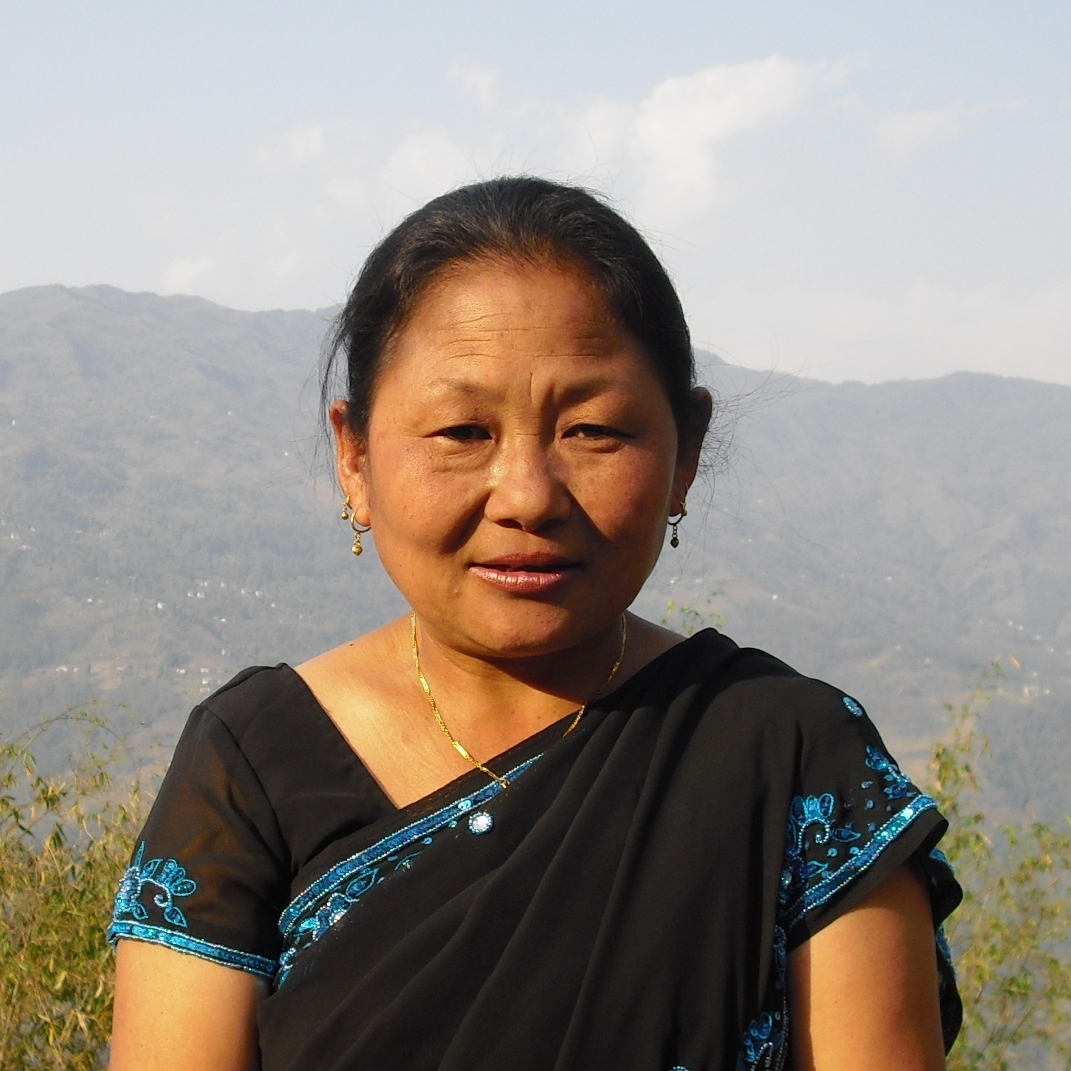
\includegraphics[width=0.30\textwidth]{kamala.jpg}
 \hfill
 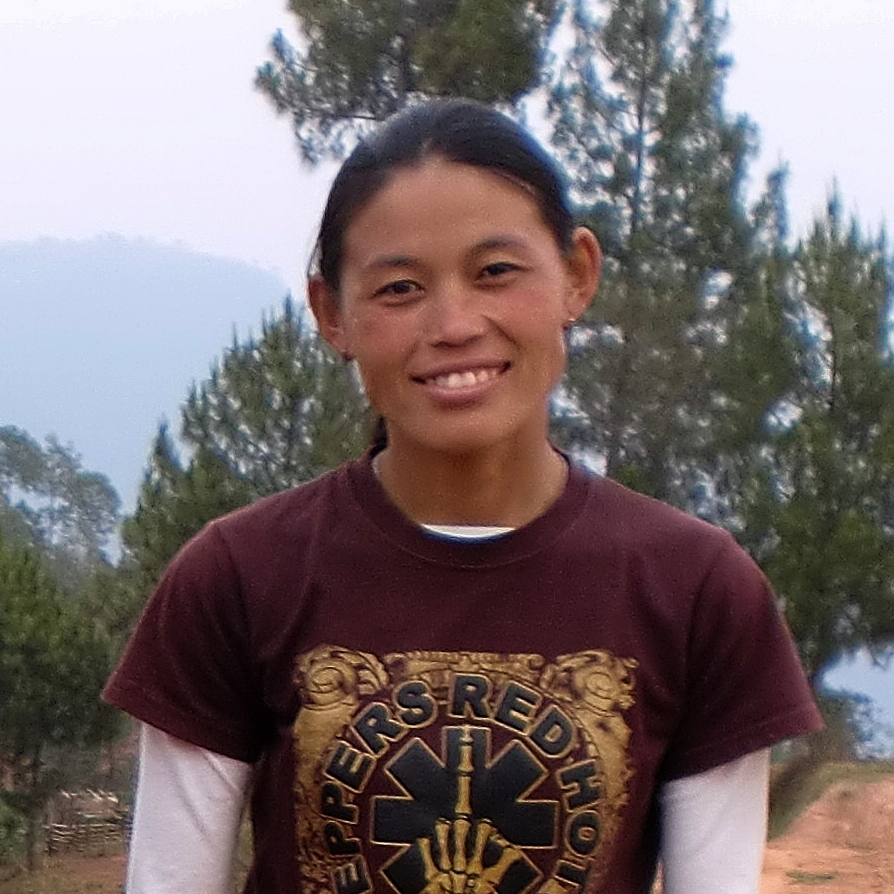
\includegraphics[width=0.30\textwidth]{manmaya.jpg}
 \hfill
 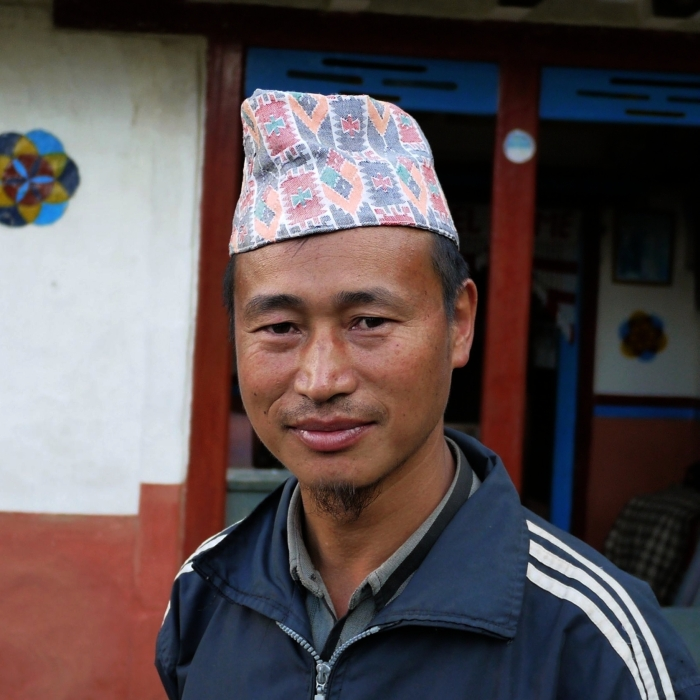
\includegraphics[width=0.30\textwidth]{magman.jpg}
 \caption{My main Yakkha teachers: Kamala Linkha, Man Maya Jimi, Magman Linkha}
 \end{figure}

 
During the early trips (2009 and 2010) I recorded texts from various genres (legendary and autobiographical narratives, spontaneous conversations, songs, pear stories, procedural descriptions) and tried to gather as much language data as possible while living in the village. In total, I recorded utterances from 22 different speakers. The youngest person recorded was 16 years old, the oldest people were above 60 years. To each person recorded I have explained the purpose of the recordings and my plan to archive them online. Their consent is mostly found as part of the recordings, usually at the end of the files.  After analyzing the data in Germany, I used the later trips (2011 and 2012) mainly for refined elicitations and data checking, with the consultants mentioned above in Tumok and in Kathmandu. 

In the elicitations, relying on nonverbal stimuli in the natural environment proved to be much more productive than prepared questionnaires or audiovisual stimuli. The only stimuli that I have used were the Pear Story \citep{Chafe1980The-Pear} and the Cut and Break Clips \citep{Bohnemeyeretal2010_cut}. Questionnaires that were used included the questionnaire from the Leipzig Valency Classes Project (Max Planck Institute for Evolutionary Anthropology), the questionnaire from the project on referential hierarchies in three-participant constructions (University of Lancaster) and the Questionnaire for Transitivizing/Detransitivizing Verb Systems (by Johanna Nichols). The other topics were elicited with questionnaires compiled by myself and on the spot when certain topics came up during transcriptions and checks of the lexical data. Elicitations on clause linkage in 2012 were partly undertaken together with Lennart Bierkandt for a co-authored paper (\citet{Bierkandtetal_Scope}).

\subsection{The corpus}\label{corpus}

The structure and content of the current Yakkha corpus is displayed in Table \ref{tab-corpus}. The corpus contains 3012 clauses and roughly 13.000 annotated words. The texts are transcribed and annotated audio-recordings of roughly 3 hours length. The audio recorder used is an Olympus Linear PCM Recorder LS-11. The texts of the genre \emph{legacy data} are only available in written form, using Devanagari script. They are taken from school books \citep{Jimi2009Engka-Yakkha, Jimi2010Engka-Yakkha} and from narratives that originated in a workshop organized in 2012 by the Mother Tongue Center Nepal \citep{Jimee2012_Casuwa, Jimee2012_Owl, Linkha2012_Ashes}. I have transliterated them into the orthographic representation used in this work, with slight adjustments where the orthographies used  were rather impractical, for instance when they lumped together the voiceless and voiced consonants or /r/ and /l/ (which is the case in the above-mentioned school books). Researchers using the corpus should be aware of the fact that many neologisms are used in written Yakkha that are not (yet) established in the spoken language. 




\begin{table}[htp]
\begin{center}
\begin{tabular}{lll}
\toprule
{\sc genre}&{\sc number of }&{\sc records}\\
& {\sc recordings}& (roughly corr. to clauses)\\
\midrule
narratives	&8&	488\\
conversations	&5&	1336\\
pear stories	&4	&225\\
songs	&3	&40\\
legacy data (written)	&5&	595\\
texts on tradition 	&3	&328\\
and material culture	&	&\\
\midrule
&28&\bf 3012\\
\bottomrule
\end{tabular}
\caption{Content of the annotated Yakkha corpus}\label{tab-corpus}
\end{center}
\end{table}


The texts are labelled as follows: a unique identifier, followed by an underscore and a three-letter genre code, followed by an underscore and the number of the text from that particular genre. For example, a text coded \rede{12\_nrr\_03.wav} is the twelfth recording in total and the third text of the genre \rede{narrative}; \rede{12\_nrr\_03.txt} is the corresponding text file. These labels (including the record number) are provided when the examples are from the corpus; when no such label is provided, the examples are from elicitations or from unrecorded spontaneous speech. The applications used for annotation and time alignment were Toolbox\footnote{Toolbox is free software developed by SIL, see http://www-01.sil.org/computIng/toolbox/index.htm.} and ELAN.\footnote{ELAN is free software developed by the Language Archive of the Max Planck Institute for Psycholinguistics in Nijmegen, see  \citet{Wittenburg2008_Annotation}; URL: http://tla.mpi.nl/tools/tla-tools/elan/;}

The genre codes are displayed in Table \ref{tab-genre}.  The entire corpus is accessible online via the Endangered Languages Archive (ELAR).\footnote{http://www.hrelp.org/archive/. The annotations in this work may, in a few cases, deviate from the annotations in the archived corpus, as upon closer inspection during the analyses some minor adjustments were inevitable. The examples as they are analyzed and annotated in this work represent the most recent state of analysis.}

\begin{table}[htp]
\begin{center}
\begin{tabular}{ll}
\toprule
{\sc code}&{\sc genre}\\
\midrule
nrr & narrative \\
cvs & conversation \\
sng & song\\
mat & description of material culture\\
tra & description of traditions\\
pea & pear story\\
par & elicited paradigm\\
leg & legacy data (written)\\
\bottomrule
\end{tabular}
\caption{Text genres and codes}\label{tab-genre}
\end{center}
\end{table}


\subsection{The lexical database}

The lexical database\footnote{Archived at the Endangered Languages Archive (ELAR) together with the corpus, see http://www.hrelp.org/archive/.} contains 2429 entries, all checked with at least two speakers. It contains grammatical, semantic, phonological and ethnographic notes as well as botanical terms (relying on the Nepali translations given in \citet{Manandhar2002_Plants} and occasionally \cite{Turner1931A-Comparative}). One may also browse for parts of speech and for semantic categories, if one is interested in particular semantic domains like body parts, kinship, spatial orientation, colour terms etc. A digital community version of the dictionary (using Lexique Pro),\footnote{See http://www.lexiquepro.com/.} with the Yakkha entries in Devanagari, can be found online.\footnote{See http://dianaschackow.de/?nav=dictionary. Even though the database has been carefully checked, it is likely that further corrections and additions will be made in the future.}


\section{Earlier studies on Yakkha language and culture}\label{earlier-work}


Material on the Yakkha language that is available beyond local sources is exceedingly rare. The oldest source is a wordlist in \citet{Hodgson1857_Comparative}. A chapter in the Linguistic Survey of India provides a brief introduction and some Yakkha texts that were collected with Yakkha speakers who had migrated to Darjeeling \citep[305-315]{Grierson1909Linguistic}.\footnote{This source and \citet{Russell1992_Yakha} use a spelling <Yakha>, but the correct spelling is <Yakkha>, since the first syllable is closed by /k/. In contemporary sources, also  in Devanagari, the language name is always written as <Yakkha>.} 

More recent works on the language are a  glossary \citep{Winter1996Glossary}, a Yakkha-Nepali-English dictionary  \citep{Kongren2007Yakkha}, two articles about the inflectional morphology, both based on the same verbal paradigm collected by Gvozdanović \citep{Gvozdanovic1987How, Driem1994The-Yakkha}, and an article by myself on three-argument constructions \citep{Schackow2012_Referential}.

Research on cultural and political aspects has been undertaken by \citet{Subba1999Politics} and by Russell \citet{Russell1992_Yakha, Russell1997Identity, Russell2000_Missing, Russell2004Traditions, Russell2007Writing, Russell2010_Perceptions}. Recently, two M.A. theses on aspects of Yakkha culture have been completed in Nepal, one thesis on culture and adaptation by \citet{Rai2011_Nature}  and one thesis on kinship terms by  \citet{Linkha2013_kinship}. Ethnographic introductions in Nepali can be found by \citet{Kongren2007Indigenous} and by \citet{Linkha2067Yakkha}, the former containing also some English chapters. Further locally available materials in Yakkha and Nepali are a collection of poems \citep{Dewan2001Opchyongme} and a  collection of thematically ordered wordlists and articles on the Yakkha traditions \citep{Linkha2005Yakkha}. For a more detailed bibliography of the works on Yakkha that were published in Nepali the interested reader is referred to \cite{Rapachaetal2008Indo}. 

 

\section{Typological overview of the Yakkha language}\label{overview-yakkha}

The following brief overview is intended for the reader who is not familiar with Kiranti languages or other Sino-Tibetan languages in general. It provides basic information on the most important features of the language.

\subsection{Phonology}

Yakkha has five vowel phonemes (/i/, /e/, /a/, /o/ and /u/). Diphthongs are rare and can mostly be traced back to disyllabic structures. The basic distinctions in the consonant phonemes, according to  the place of articulation, are bilabial, alveolar, retroflex, palatal, velar and glottal. Plosives, the affricate and the bilabial glide have an aspirated and an unaspirated series. The maximal syllable structure is CCVC. Complex onsets originate in disyllabic structures too; they consist of sequences of obstruent and lateral, rhotic or glide. The syllable coda is mainly restricted to nasals and unaspirated plosives. The morphophonological processes are manifold and very complex in Yakkha, with each rule applying to its own domain (discussed in §\ref{morphophon}). A feature located at the boundary between phonology and morphology is a process of copying nasal morphemes in the verbal inflection (discussed in §\ref{sec-nasalcop}). This process is typical for Kiranti languages.


\subsection{Word classes}

Morphology and syntax clearly distinguish nominal and verbal classes in Yakkha (see Chapters \ref{ch-noun} and \ref{verbalmorph}). Word classes appearing in the noun phrase are demonstratives, pronouns,  quantifiers and (marginally) numerals (see Chapter \ref{ch-pron}). Numeral classification exists, but it plays only a very marginal role. The verb shows complex inflectional morphology, resulting in hundreds of possibilities of inflection for each verbal stem. 


Less clear is the distinction of adjectives and adverbs, as many of them derive from verbal roots. However, the salience of reduplication and rhyming patterns in noun-modifying and verb-modifying lexemes justifies treating them as separate word classes (see Chapter \ref{adj-adv}). Rhyming and reduplications, often combined with ideophones, almost exclusively feature in the classes of adjectives and adverbs in Yakkha.


Other word classes constitute closed classes, such as conjunctions, postpositions, interjections and discourse-structural particles (see Chapters  \ref{clink-rest} and \ref{particles}). The postpositions are partly derived from relational nouns. 


\subsection{Nominals}

Yakkha nouns can be simple or compounded out of several nominal roots. There are several nominalizers in Yakkha, some deriving nouns (\emph{-pa} and \emph{-ma}), some constructing noun phrases (\emph{-khuba, -khuma} and \emph{=na/=ha}).

 Nouns can be inflected by possessive prefixes, alternatively to using possessive pronouns (compare \Next[a] and \Next[b]). The possessive prefixes are very similar in form to the possessive pronouns. Case and number markers are clitics; they attach to the whole noun phrase. Yakkha has an unmarked nominative, an ergative/instrumental \emph{=ŋa}, a genitive \emph{=ka}, a locative \emph{=pe}, an ablative \emph{=phaŋ}, a comitative \emph{=nuŋ}, and further markers with less central functions, mainly from the comparative domain. Argument marking shows reference-based and word class-based alternations (discussed in §\ref{nom-morph} for the ergative case and in §\ref{three-arg} for three-argument constructions).

\ex.\ag.a-paŋ=be\\
{\sc 1sg.poss-}house{\sc =loc}\\
\rede{in my house}
\bg.ak=ka paŋ=be\\
{\sc 1sg.poss=gen} house{\sc =loc}\\
\rede{in my house}


\subsection{Verbs}

The inflected verb  indexes agents and patients of transitive verbs and expresses many grammatical categories (tense/aspect, mood, polarity (see \Next). This example also shows the above-mentioned process of nasal copying; suffix \emph{-m} appears twice in the suffix string. Person (including clusivity), number and syntactic role marking interact in intricate ways in the person marking paradigm (see §\ref{verb-infl}). As example \Next shows, the Yakkha verb is mainly suffixing; there is only one prefix slot. 

\exg.n-dund-wa-m-ci-m-ŋa-n=ha\\
{\sc neg-}understand{\sc -npst-1pl.A-nsg.P-1sg.A-excl-neg=nmlz.nsg}\\
\rede{We do not understand them.}


Yakkha has a very productive system of complex predication, where several verbal roots are concatenated to yield a more specific verbal meaning (discussed in Chapter \ref{verb-verb}). In complex predicates, the first verb carries the lexical meaning, while the second verb adds a further semantic specificiation, for instance regarding aktionsart, the spatial directedness of the event, or the affectedness of some argument. In \Next, the second verb carries a benefactive notion, adding a beneficiary argument to the argument structure of the lexical verb. Complex predicates trigger recursive inflection, as shown here by the imperative marker \emph{-a}, that appears twice (treated in detail in Chapter \ref{verb-verb}). Predicates can also be compounded by a noun and a verb  (see Chapter \ref{noun-verb}).
 	
	\exg. ka katha lend-a-by-a-ŋ\\
	{\sc 1sg} story  exchange{\sc -imp-V2.give-imp-1sg.P}\\
	\rede{Tell me a story.}



\subsection{Syntax}

Yakkha phrase structure is overwhelmingly  head-final, with the nominal head at the end of the noun phrase, and with the verb being the final constituent of the clause (see \Next[a]). In complex clauses, the subordinate clause generally precedes the main clause (see \Next[b]). Nominalizers and markers of clause linkage can follow the verb. Permutations of the word order are possible (see Chapter \ref{simp-cl}); they follow discourse requirements. Arguments are frequently dropped, resulting in a low referential density. 

\ex.\ag.raj=ŋa u-ma  kheps-u=na\\
Raj{\sc =erg} {\sc 3sg.poss-}mother hear{\sc [pst]-3P=nmlz.sg}\\
\rede{Raj heard his mother.}
\bg.tumok=pe tas-u-ŋ=hoŋ a-phu chimd-u-ŋ=na\\
Tumok{\sc =loc} arrive{\sc [pst]-3P-1sg.A=seq} {\sc 1sg.poss-}elder\_brother ask{\sc [pst]-3P-1sg.A=nmlz.sg}\\
\rede{When I arrived in Tumok,  I asked my elder brother (about it).}

The argument structure in Yakkha distinguishes several valency classes, discussed in Chapter \ref{verb-val}. The basic distinction is that between intransitive and transitive verbs, which is also reflected in two different verbal inflectional patterns. There is a class of labile verbs, mostly showing an \emph{inchoative/causative} alternation. Experiential predicates predominantly occur in a construction that treats the experiencer as the metaphorical possessor of a sensation or an affected body part (the Experiencer-as-Possessor Construction, see \Next).

\ex.\ag.a-pomma=ci ŋ-gy-a=ha=ci\\
{\sc 1sg.poss-}laziness{\sc =nsg} {\sc 3pl-}come\_up{\sc -pst=nmlz.nsg=nsg}\\
\rede{I feel lazy.}
\bg.ka nda         a-luŋma  tuk-nen=na\\
{\sc 1sg[erg]} {\sc 2sg} {\sc 1sg.poss-}liver pour{\sc -1>2[pst]=nmlz.sg}\\
\rede{I love you/I have compassion for you.}


The argument structure can be modified, by means of derivations (causative), complex predication (benefactive, middle, reflexive), and an analytical construction (reciprocal), as shown in \Next. Both the  reflexive and the  reciprocal construction make use of a grammaticalization of the verbal root \emph{ca}  \rede{eat}. 


\ex.\ag.kiba=ŋa hari kisi-met-u=na\\
tiger{\sc =erg} Hari be\_afraid{\sc -caus-3.P[pst]=nmlz.sg}\\
\rede{The tiger frightened Hari.}
\bg. nda (aphai) moŋ-ca-me-ka=na\\
\sc{2sg} (self) beat-\sc{V2.eat-npst-2=nmlz.sg}\\
\rede{You beat yourself.}
\bg. kanciŋ [...] sok-khusa ca-ya-ŋ-ci-ŋ\\
\sc{1du}  [...] look-\sc{recip} eat\sc{.aux-pst-excl-du-excl}\\
\rede{We (dual, excl) looked at each other.}



Furthermore, morphologically unmarked detransitivizations are possible (marked only by a change in the person marking morphology). In this way, both antipassive and passive constructions may occur in Yakkha, sometimes leading to ambiguities. In \Next, the person morphology on the verb is intransitive in both examples, signalling a third person singular subject of an intransitive verb, although \emph{khemma} \rede{hear} is clearly transitive, and in most cases is inflected transitively (compare with \Next[c]). While \Next[a] is a passive structure, \Next[b] is an antipassive. Unmarked antipassives (the morphosyntactic demotion of a generic or unspecific object) are wide-spread in Kiranti languages, but unmarked passives are, to this point, only known in Yakkha. The more frequent structure is, however, the antipassive, which is not surprising given its older nature.

\ex.\ag. ceʔya kheps-a-m=ha\\
matter hear{\sc [3sg]-pst-prf=nmlz.nc}\\
\rede{The matter has been heard.}
\bg. Dilu  reɖio khem-meʔ=na?\\
Dilu radio  hear{\sc [3sg]-npst=nmlz.sg}\\
\rede{Does Dilu listen to the radio (generally)?}
\bg. pik=ŋa kiba kheps-u=na\\
cow{\sc =erg} tiger hear{\sc [pst]-3P=nmlz.sg}\\
\rede{The cow heard the tiger.}



Yakkha does not have a dominant grammatical relation, both reference-based and role-based (ergative, accusative) alignment patterns are found, depending on the particular construction. Especially the verbal person marking system shows an incredible heterogeneity of alignment types, which is, however, not unusual in a Kiranti-wide perspective (see Figure \ref{aligntables} on page \pageref{aligntables}). 

Nominalization is a core feature of Yakkha syntax (discussed at length in Chapter \ref{ch-nmlz}). The nominalizers have a wide range of functions, from nominal modification/relativization and complement clauses to marking independent clauses. The nominalizers \emph{-khuba} and \emph{-khuma} construct noun phrases (and relative clauses) with the role of S or A, while the nominalizers \emph{=na} and \emph{=ha} are almost unrestricted with regard to which participant they can relativize on (see \Next). The only relation not found with relative clauses in \emph{=na} or \emph{=ha} is A, which results in syntactic ergativity for relative clauses, since S and P are treated alike by this relativization and differently from A.
The nominalizers \emph{=na} and \emph{=ha} are also frequently used to nominalize independent clauses, with the function of structuring information  on the text level (see Chapter \ref{nmlz-uni-3}). 

\ex. \ag.   heko=ha=ci mok-khuba babu\\
			other{\sc =nmlz.nsg=nsg} beat{\sc -nmlz} boy\\
			\rede{the boy who beats the others} 
\bg.nna  o-hop wa-ya=na siŋ\\
		that {\sc 3sg.poss}-nest exist-{\sc pst[3sg]=nmlz.sg} tree\\
	\rede{that tree where he has his nest} 
	

Complement constructions show long-distance agreement, distinguishing various subtypes, each with its own configuration of person  and case marking (see Chapter \ref{compl}). There are two basic types: infinitival complement clauses and inflected complement clauses (see \Next). In this particular example, the same complement-taking verb \emph{miʔma} acquires two separate meanings, depending on whether the embedded structure is infinitival or consists of an inflected verb.

\ex.\ag.ka kheʔ-ma mit-a-ŋ=na\\
{\sc 1sg} go{\sc -inf} think{\sc -pst-1sg=nmlz.sg}\\
\rede{I want to go.}
\bg. nda cama ca-ya-ga=na mi-nuŋ-nen=na\\
{\sc 2sg[erg]} rice eat-{\sc pst-2=nmlz.sg} think-{\sc prf-1>2=nmlz.sg}\\
\rede{I thought you ate the rice.} 


Adverbial clause linkage has three major types: infinitival clauses (see \Next[a]), converbs (see \Next[b]) and inflected adverbial clauses (see \Next[c]). The subtypes of these three basic types are discussed in detail in Chapter \ref{adv-cl}. Further conjunctions can connect clauses on the text level, such as \emph{khaʔniŋgo} \rede{but} and \emph{nhaŋa} \rede{and then, afterwards}.

\ex.\ag.uŋci=ŋa men-ni-ma=ga cum-i\\
{\sc 3nsg=erg} {\sc neg-}see{\sc -inf=gen} hide{\sc -1pl[pst]}\\
\rede{We hid, so that they would not see us.} 
\bg.	o-pomma ke-saŋ ke-saŋ kam cog-wa\\
	{\sc 3sg.poss-}laziness come\_up-{\sc sim} come\_up-{\sc sim} work do{\sc -npst[3sg.A;3.P]}\\
		\rede{He does the work lazily.}
\bg. ka kucuma khas-a=nuŋ pi-ŋ=ha\\
{\sc 1sg[erg]} dog   be\_satisfied{\sc [3sg]-sbjv=com.cl} give{\sc [pst;3.P]-1sg.A=nmlz.nsg}\\
\rede{I fed the dog sufficiently (in a way that it was satisfied).}






%  \chapter{The Yakkha language and its speakers}\label{languageintro}
\todo{Please use only exhaustive sections; See Generic Style Rules pg 2}
This chapter provides basic information on the geographic (\sectref{geogr}) and cultural-historical  background of the Yakkha language (\sectref{cult-hist}), a genealogical classification of Yakkha as a member of the Kiranti language family (\sectref{genetic}), and its sociolinguistic (\sectref{socioling}) context. The reader should note that the  following observations are not made by a trained anthropologist. An in-depth anthropological study is beyond the scope of this introductory chapter (see \sectref{earlier-work} for existing anthropological studies). 

In this chapter, the term  Kiranti can indicate both ethnic and linguistic affiliations. It refers to a group of roughly 30 ethnically and linguistically distinct, yet related, communities in eastern Nepal. The internal structure of the Kiranti group is complex, and linguistic classifications may deviate from ethnic classifications, cf. \sectref{cult-hist} below.

\section{Geographical context}\label{geogr}

Nepal can roughly be divided into three geographical zones: the Himalayan range in the north, the middle hills (the Mahabharat range, stretching parallel to the Himalayan range) and the plains in the south (the Tarai). The Himalayan range is home to speakers of Tibeto-Burman languages. The plains are mostly inhabited by speakers of Indo-Aryan languages. Furthermore, a few Austroasiatic languages, one Dravidian language and an isolate (Kusunda) are spoken in Nepal. Speakers of Kiranti languages, including Yakkha (see \figref{nepalmap}), inhabit the hilly area between the Likhu river in the west and the border with Sikkim in the east, with elevations between 1,500m and 2,700m. Kiranti  settlements can also be found in the plains and in India (Darjeeling, Sikkim). 

\begin{figure}
\centering
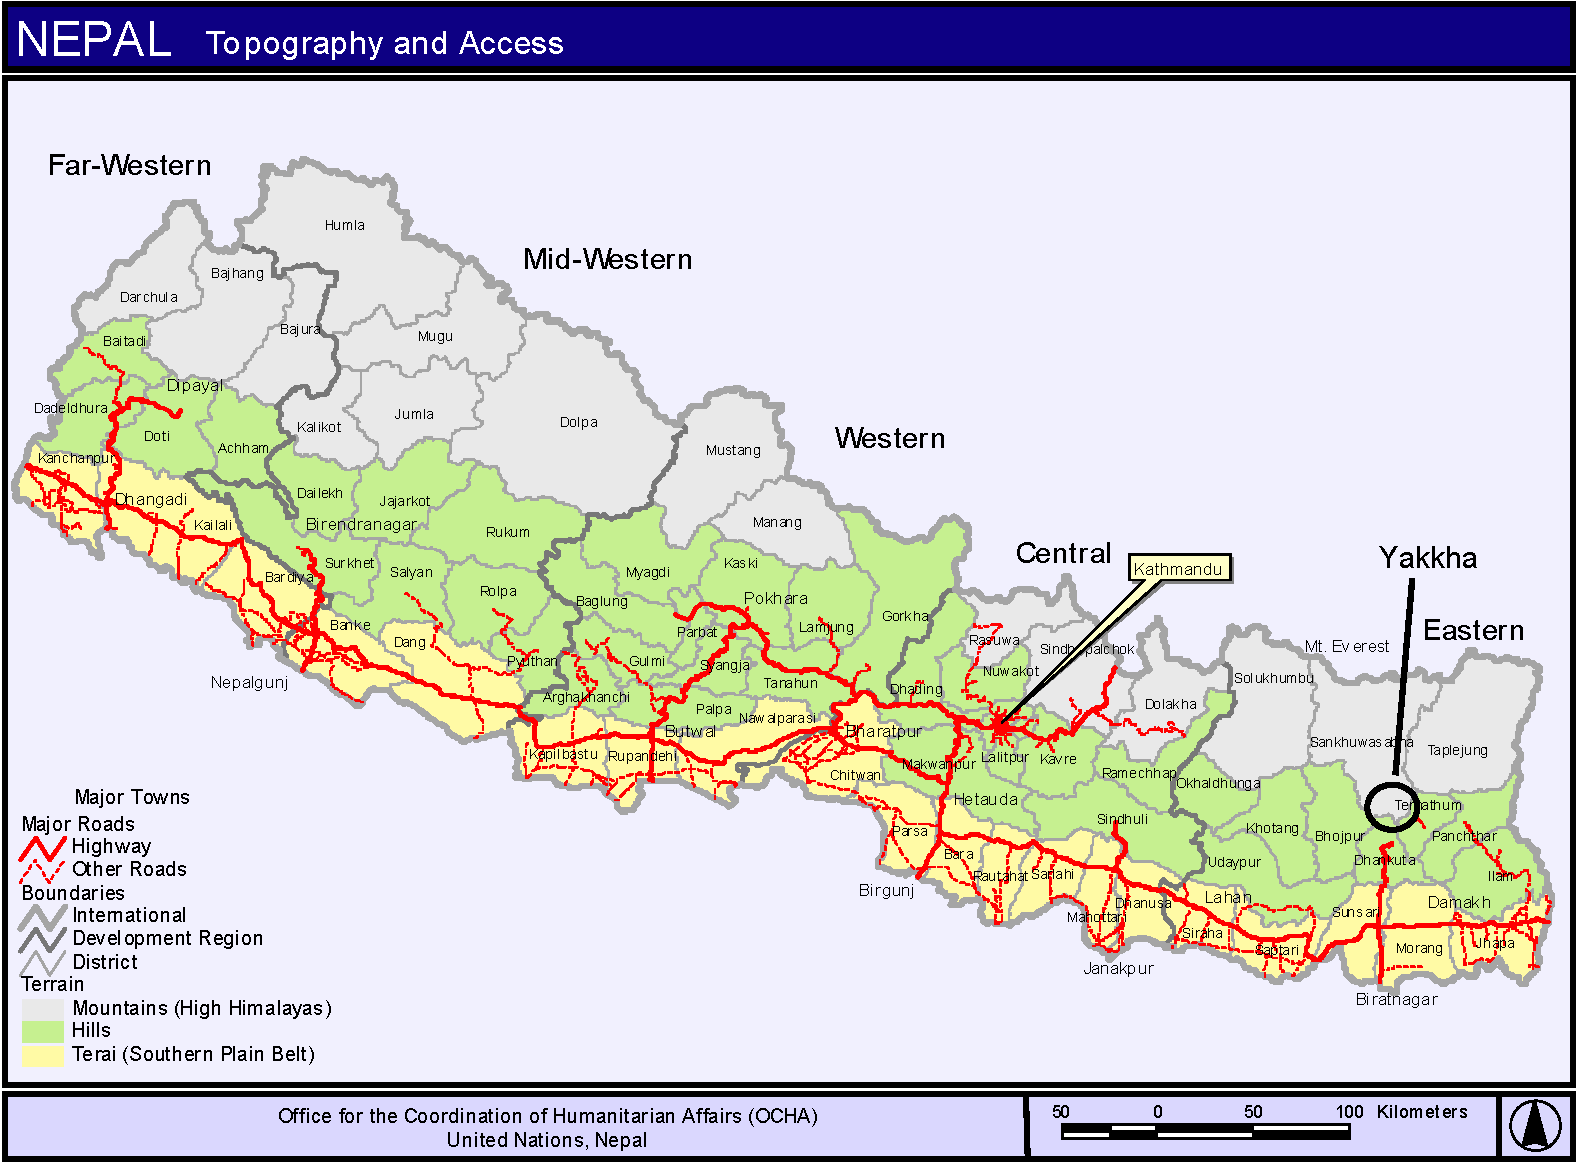
\includegraphics[width=11cm]{figures/Nepalkarte.pdf}
\caption{Location of the Yakkha region within Nepal (United Nations Map Centre: http://www.un.org.np/resources/maps, accessed on 17 January 2014 )}\label{nepalmap}
\end{figure}

The Yakkha region (i.e. the area inhabited by people who consider themselves Yakkha ethnically)\footnote{If the region were defined by linguistic criteria, it would be much smaller; see \sectref{endangerment}.} is located in the Koshi zone of the Eastern Development Region, in the south of Sankhuwa Sabha district and in the north of Dhankuta  district  (see the maps in \figref{map-sank} and \figref{map-dhan}). Within the region in  Eastern Nepal commonly known as \emph{Kirant} (\rede{Kiranti area}), the Yakkha region belongs to the \emph{Pallo Kirant} \rede{Far Kiranti area}, located on the east of the Arun river. 

The core Yakkha region contains the following Village Development Commitees (\textsc{vdc}s):\footnote{Nepal is administratively divided into 5 development regions, 14 zones, 75 districts and  3,913 village development commitees (\textsc{vdc}s). Each \textsc{vdc}  contains several villages and is further divided into numbered wards.} Canuwa, Marek Katahare and Dandagaun in Dhankuta district, and Tamaphok (Tamfok in the map), Mamling, Ankhinbhuin, Madi Mulkharka, Madi Rambeni, Baneshwor, Chainpur, Kharang, Wana (Bana in the map), Siddhakali, Siddhapokhari and Syabun in Sankhuwa Sabha district. The Yakkha region is also known as the \emph{Tin Thum} (\rede{The Three Regions}): the \emph{Das Majhiya} in the south, the \emph{Panch Majhiya} in the middle and the \emph{Panch Kapan} in the north  \citep[86]{Kongren2007Indigenous}, a distinction originating in the tax system that was enforced under the Gorkha rule in the 18\textsuperscript{th} century. The language is  only spoken by parts of the Yakkha population, being replaced by Nepali in almost half of the geographic area inhabited by Yakkha people. Curiously, the language proficiency decreases drastically towards the north of the Yakkha area (Magman Linkha, p.c.), contrary to the expectation that greater distance to the main roads and thus greater isolation should have had a positive effect on the preservation of a language. 



\begin{figure}
\centering
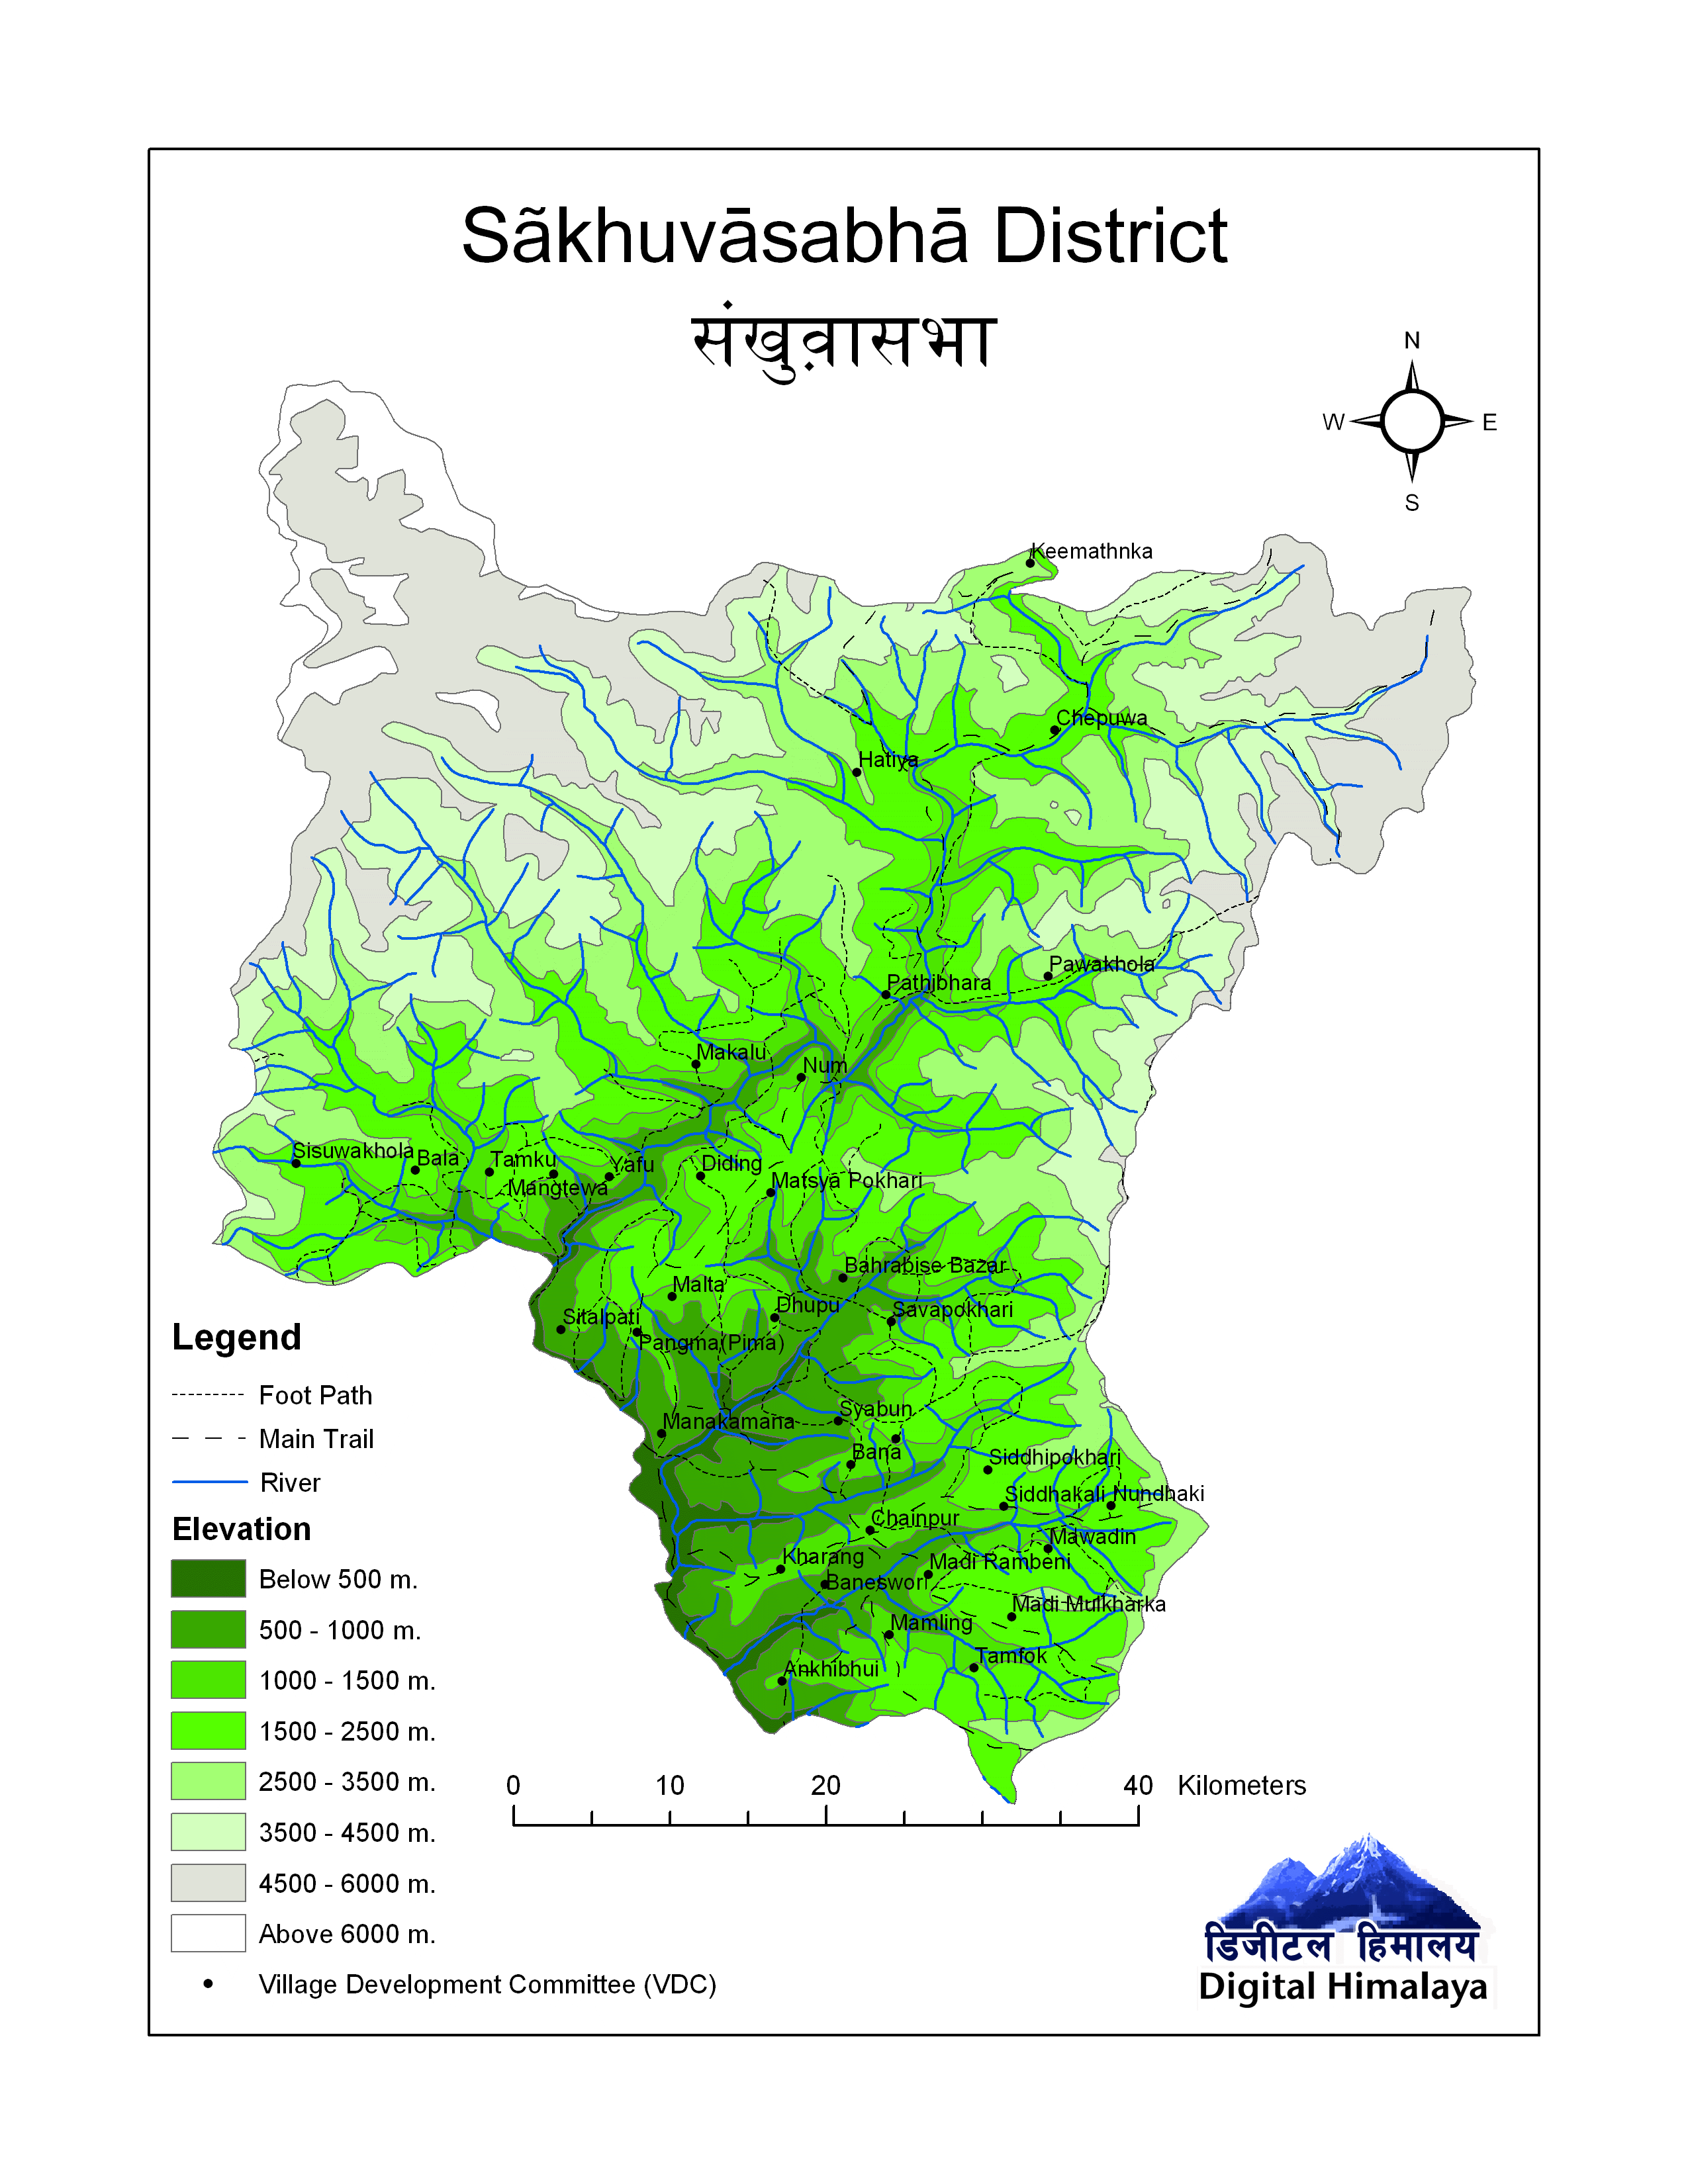
\includegraphics[height=15cm]{figures/district_sankhuwasabha_everything.png}
\caption{Map of Sankhuwa Sabha district, with Yakkha villages in the south \citep{Joshi_Nepal_maps}}\label{map-sank}
\end{figure}

\begin{figure}
\centering
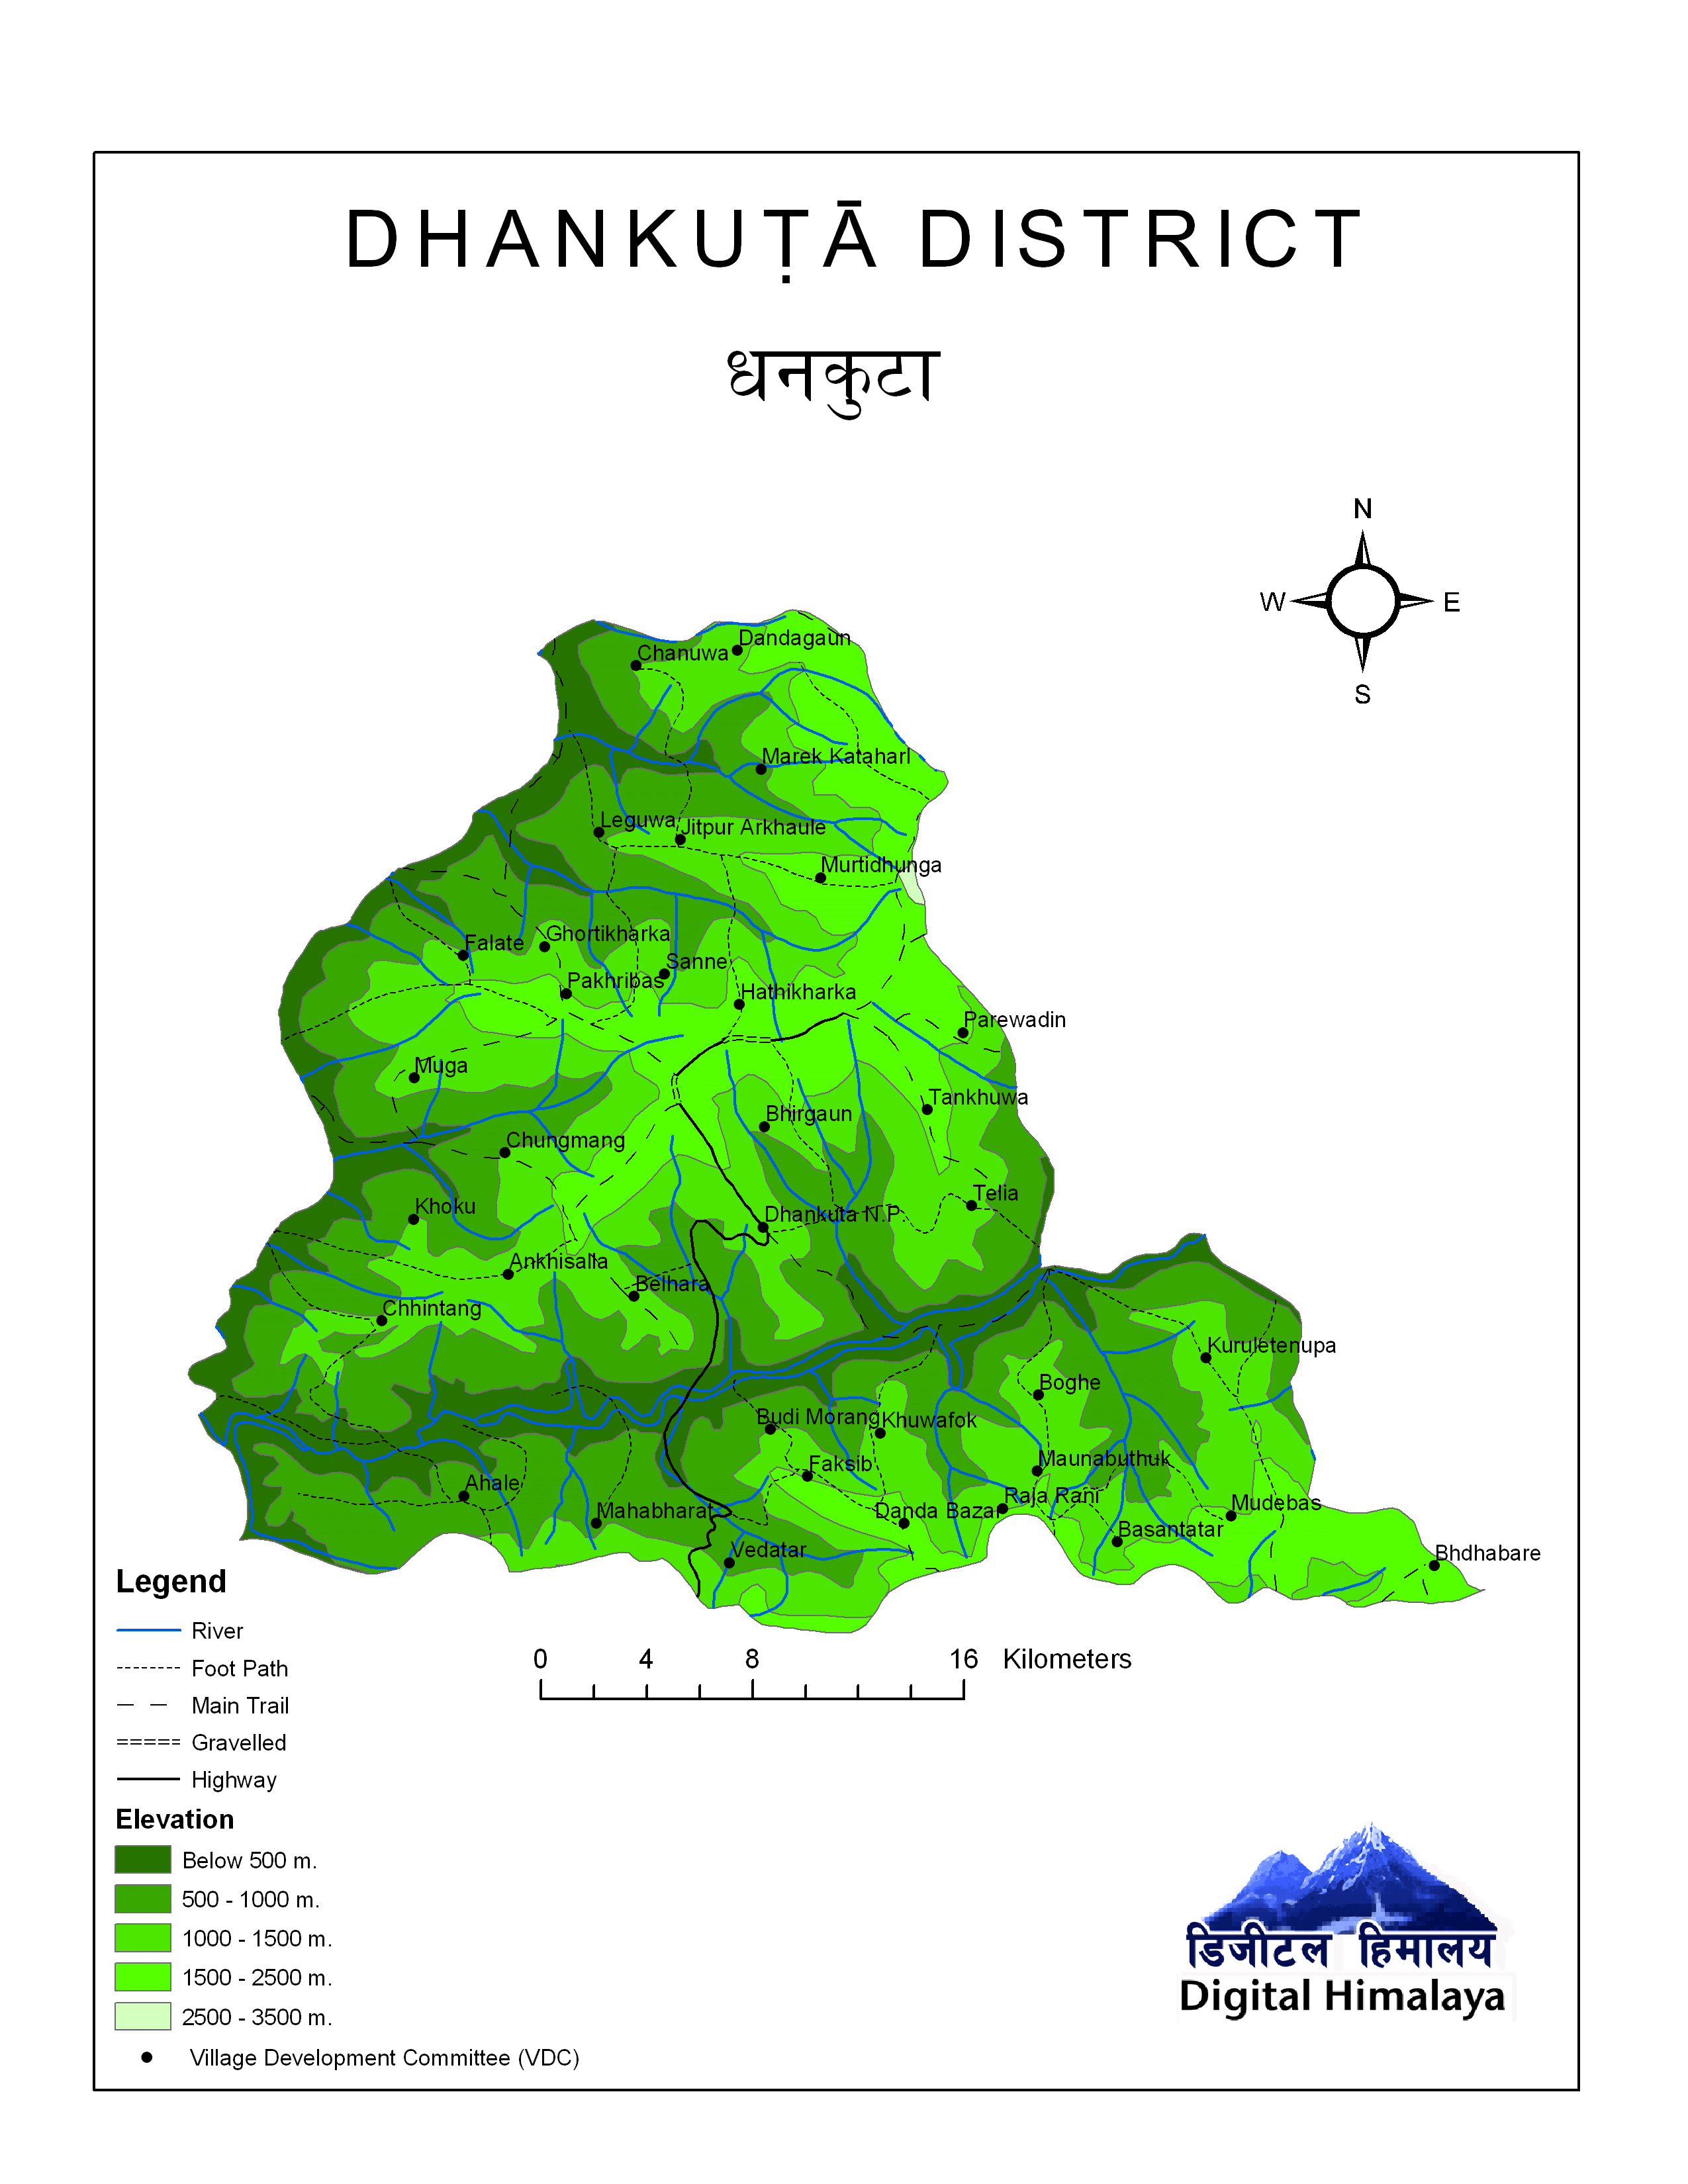
\includegraphics[height=15cm]{figures/district_dhankuta_everything.png}
\caption{Map of Dhankuta district, with Yakkha villages in the north \citep{Joshi_Nepal_maps}}\label{map-dhan}
\end{figure}

Yakkha has at least four dialects (see \sectref{sc-dialect} below). The focus of this work is on the Tumok dialect, named after the village where it is spoken (27.208°N, 87.384°E), in Tamaphok \textsc{vdc}.\footnote{Tamaphok is also the Nepali name of Tumok. Many Yakkha villages have both a Nepali name and a Yakkha name. Impressionistically, Yakkha names are used to refer to particular villages, while  Nepali names are used to refer  to \textsc{vdc}s (which are in general conglomerations of several villages). This is also the case e.g. for Waleng (Nepali: \emph{Madi Mulkharka}), Yaiten (Nepali: \emph{Dandagaun}) and Angbura (Nepali: \emph{Omruwa}).} Tumok  lies on the south-western slopes of the Maya Khola valley.\footnote{\emph{kholā} is a Nepali word for \rede{little river}.} The Maya Khola flows north-west into the Piluwa Khola, which is a tributary of the Arun river (the main river in the region, partly flowing along the south-western border of Sankhuwa Sabha district). Tumok  is located approximately 1500m above sea level. Villages in this hilly region generally spread over several hundred meters of altitude, because the houses are not built close to each other, allowing space for fields between them. The great extension of the villages may lead to climatic differences and to differences in the crop cycle even within one village. The speaker density in Tumok is very high, and even parts of the non-Yakkha population speak Yakkha in addition to Nepali.\footnote{Among the non-Yakkha population, it is more common to speak Yakkha for members of castes that were perceived as “low” (according to Hindu social law)  than for members of so-called “high” castes. Despite changes in the legal system, these distinctions still play a role in social practice and thus, it is more attractive for members of discriminated groups to learn Yakkha, while members of “high” castes often do not know any Yakkha, even after having lived in the area for decades.} \figref{tumok} shows the view from Tumok towards the Himalayan range in the north. 

\begin{figure}
\centering
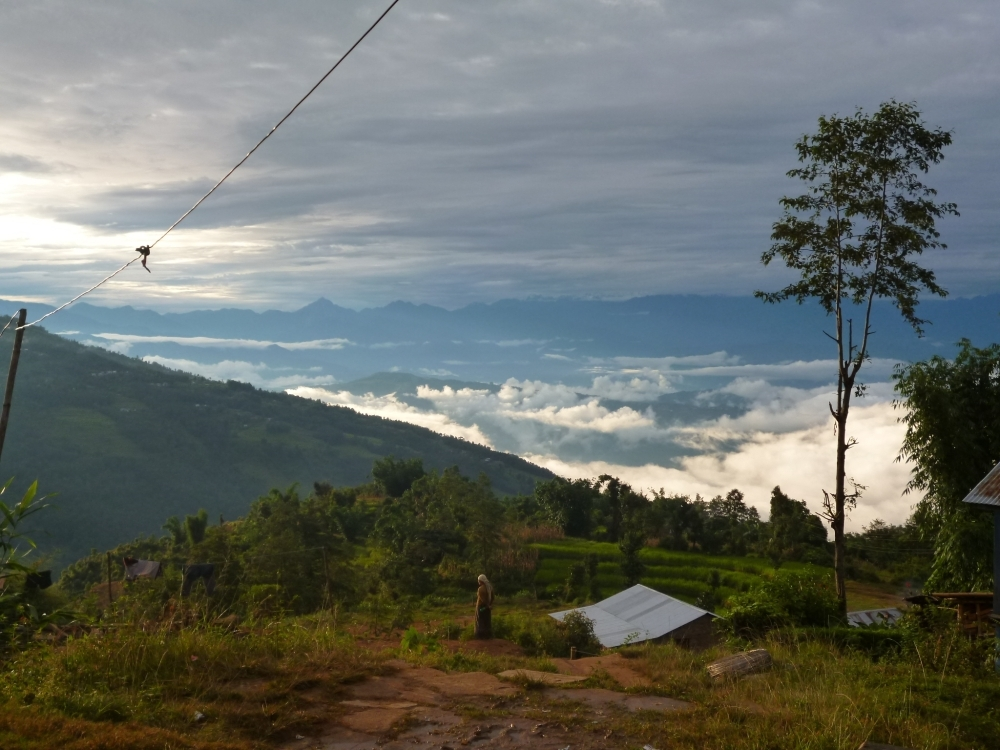
\includegraphics[width=10cm]{figures/tamaphok.jpg}
\caption{Tumok at the end of the rainy season, Sept. 2012}\label{tumok}
\end{figure}
 

Yakkha speakers can also be found outside the core area defined above. There are about 80 households in the south-east of Dhankuta district, in Mudhebas \textsc{vdc}, Kuruletenupa \textsc{vdc} and Bodhe \textsc{vdc} (Magman Linkha, p.c.). In Ilam district, a Limbu-speaking region bordering with India, Yakkha speakers are reported to live in Namsaling village, speaking a dialect that is perfectly intelligible with the Yakkha from the core area. Nowadays there are also many Yakkha people living outside the hills, in the city of Dharan (Sunsari district) and other places in the Tarai and in India (especially in Darjeeling and Sikkim). A common reason for migration is the search for land or employment. Of course, Yakkha are also found elsewhere in the world due to the high rate of Nepali emigration for the previously mentioned reasons as well as education. 

The Yakkha region is surrounded by other Kiranti languages. Going clockwise, starting in the east, these are Limbu (including the Tamarkhole, Phedappe  and Chatthare dialects). Athpare,  Chɨlɨng, Belhare and Chintang follow in the south, Bantawa and Dungmali in the west, Mewahang, Lohorung and Yamphu in the north. This geographical classification has to be understood in an idealized sense. Most of the villages in Nepal are ethnically and linguistically diverse, so that one may also find Sherpa, Gurung, Tamang, Newari and Parbatiya (Nepali speaking) households in the Yakkha region.

  

\section{Cultural and historical background}\label{cult-hist}

\subsection{Kiranti}


Kiranti (also Kirāt, Kirāta, Kirā̃ti) nowadays refers to a set of roughly 30 communities speaking related languages, who inhabit the Himalayan foothills in Eastern Nepal and share key cultural practices, including nature worship and a body of oral knowledge, myth and ritual in which the veneration of ancestors plays a major role (known as \emph{Munthum} in Yakkha). Within these parameters, however, there is considerable heterogeneity of cultural practices, beliefs and origin myths, and shifting ethnic and linguistic affinities do not seem to be uncommon (Yakkha itself being a prime example, as will be explained further below).\footnote{Although this is commonly overlooked in current politics in Nepal,  present-day ethnic distinctions are the product of several waves of migrations and millenia of mutual influence in the Himalayan contact zone of Indosphere and Sinosphere (terms from Matisoff, e.g. \citealt{Matisoff1990_On}). The perception of distinct “pure” and time-stable ethnic and linguistic groups presents a highly idealized picture that does not do justice to the complex social reality of a multi-ethnic country like Nepal. Most current ethnic identities have been shaped by mixing with other groups or by adapting to other groups in one way or another, and these processes are, of course, continuing in the present.} 

We have very little historically verified knowledge about the Kiranti people.\footnote{The work of renowned Limbu historiographer Iman Singh \citet{Chemjong1967History}, widely perceived as the major source on Kiranti history among the Kiranti people, uses the available sources (both western scholarly work and indigenous chronicles) with few epistemological criticisms, and does not provide sufficient evidence to be called historical in the academic sense. It is rather to be seen as an attempt to anchor Kiranti culture in the deepest past possible and the widest  area possible, with  evidence spanning large parts of Eurasia from Greece to Cambodia \citep[125]{Schlemmer2003_New}. Despite its methodological shortcomings, Chemjong's work must be praised for its contribution to the acknowledgement and recognition of a distinct and unique Kiranti culture (see also \citealt[340]{Gaenszle2002_Remaking}).} The term Kiranti comes from Sanskrit \emph{kirāta} and dates back to Vedic texts such as the Atharvaveda, which is considered the oldest Veda after the   R̥gveda \citep[594]{Driem2001Languages}. It is generally accepted by Nepali and foreign historians alike that kings known as Kiranti (or Kirāta) must have ruled over central Nepal before they were overthrown by the Lichhavis early in the first millenium CE \citep[13]{Whelpton2005A-History}.  However, the well-documented history of Nepal unfortunately only begins with the Lichhavi dynasty, so that it is not at all clear whether the ancient Kirantis were the forefathers of the Kiranti people who currently live in eastern Nepal. One should note that in  the old Indian texts the term \emph{kirāta} had a much broader reference, applying to Tibeto-Burman hill peoples in general \citep{Whelpton2005A-History, Schlemmer2003_New}. The self-designation Kiranti in the present sense came to be used only with the advent of the Gorkha kings, when a common Kiranti identity began to evolve under Hindu dominance \citep[340]{Gaenszle2002_Remaking}. Before that era, there was no common feeling of being Kiranti: clan affinities were most important, and autonyms such as Khambu/Khombo (for the Rai) and Yakthumba (for the Limbu) were used among the Kiranti groups.


Present-day Kiranti legends trace the groups' origins to a variety of locales, from Tsang in Tibet to Varanasi in the Gangetic plains (see \citealt[xix]{Driem1987A-grammar} for Limbu), or places in the Tarai (see \citealt[34]{Gaenszle2012_Where} for Mewahang).\footnote{The Yakkha legends I recorded are about their ancestors' deeds and journeys in the area where present-day Yakkha people live. My own materials do not contain myths regarding a prior place of origin. This does not imply that there are no such myths. I have recorded only eight narratives, which is probably not even close to representative of what is still out there, unrecorded. In general, the Kiranti groups have a strong concern for the past and vibrant oral traditions in which origins and migrations are recalled for many generations \citep{Gaenszle2000Origins, Gaenszle2002_Remaking}.} It is not known when and how the ancestors of the Kiranti groups entered Nepal, but it is very likely that they came at least 2000 years ago from the east \citep{Driem2001Languages, LaPolla2001_Role, Gaenszle2002_Remaking}. Kiranti languages show striking similarities with rGyalrongic languages spoken in the South of China and with the extinct Tangut language, especially with regard to hierarchical patterns in the person marking system (see e.g. \citet{DeLancey1981_Category, Ebert1990Evidence, LaPolla2007Hierarchical, Jacques2012_Agreement}, and also \sectref{verb-infl} and \sectref{obl} of this work), although direct contact between these  groups has not been proven.\footnote{There is a scholarly debate as to whether these similarities are Proto-Tibeto-Burman (and got lost in the other languages) or whether the groups showing hierarchical patterns in person marking form a separate branch of Tibeto-Burman (see e.g. \citealt{Driem1991Tangut, LaPolla2001_Role, DeLancey2010_Towards, Jacques2012_Agreement, LaPolla2012_Comments}). The debate boils down to the still unsettled question of whether Proto-Tibeto-Burman had person marking morphology or not, and it will probably only be settled once more data on Tibeto-Burman languages are available.} Another argument for  migration from the east is that those Tibeto-Burman groups that have entered Nepal via the north, such as the Tamangs for instance, show a close relation to Tibetan culture and Tibetan Buddhism \citep{LaPolla2001_Role}, while Kiranti culture is clearly distinct from Tibetan culture.\footnote{To provide a culinary example: fermented soybeans (\emph{kinama} in Yakkha) are an integral part of the Kiranti cuisine. While this dish is not widely cherished outside the Kiranti sphere in Nepal, it is widespread in Northeast India (e.g. in Nagaland), and  also known from Thailand, Burma, Korea and Japan \citep{Tamang2010_fermented}.} 
%in Jacques: Baumann 1975, DeLancey 1981, van Driem 1993, Ebert 1990
 
The Kiranti peoples' more recent history has been described in various sources  \citep{Caplan1970_Land, Pradhan1991The-Gorkha, Gaenszle2002_Remaking, Schlemmer2003_New, Whelpton2005A-History} and will  only be briefly summarized here. As a nation state, Nepal was founded by Pr̥thvī Nārāyaṇ Śāha (1723--1775), the king from Gorkha\footnote{Gorkha is a district in the Western Development Region of Nepal.} who conquered the area known as Nepal today. Seen as a hero by Nepali nationalists, for the ethnic minorities his name stands for the suppression of their cultures and languages. Local groups confronted the king and his successors with strong armed resistance, but eventually Gorkha rule was established. The Kiranti region, bordering British-ruled Sikkim in the East, was critical to maintaining the Gorkha rule, and in order to keep the Kiranti groups loyal, they were given a privileged status and a certain degree of autonomy. In a system known as \emph{kipāt}, land rights were reserved for Kiranti people who owned the land by virtue of their ethnic affiliation. Local headmen were appointed to collect taxes. The titles given to them (Rai, Subba, Jimdar) are still reflected in contemporary Kiranti surnames. Later, the Gorkha kings changed their strategy and sought to control and assimilate the Kiranti region. Kiranti groups were officially incorporated into the caste system (as \emph{matvāli jāt}, \rede{drinking caste}), and the state encouraged Hindu settlers to move east. They were allowed to take control of land previously held by Kiranti people, thus systematically undermining the \emph{kipāt} system. Brahmanic values became more influential, Nepali was propagated as the national language and attempts to express and preserve one's ethnic identity were suppressed as threats to the nation state. On an everyday level,  obviously some expression of \rede{Kiranti-ness} must have continued, because distinct Kiranti cultural practices are still present nowadays (see also the observations made by \citealt{Russell2004Traditions}).
 
Hindu dominance began to erode only recently, with the 1990 constitution, in which Nepal's multi-ethnic and multi-lingual social reality was officially acknowledged for the first time (Article 4), and more so since the end of the monarchy in 2006. Currently, a new and strong sense of a common Kiranti identity is emerging, which can be attributed to the recent climate of rising ethnic consciousness (over the last two decades). The different Kiranti groups (Limbu, Rai, Yakkha, Sunwar) now share a newly-built temple in Sāno Hāttiban in the south of Kathmandu and they celebrate festivals together that were originally celebrated separately, on
village level.\footnote{Cf. \citet{Gaenszle_Redefining} on the changes that Kiranti culture and religion are currently undergoing now that more and more people live outside the rural homeland.}  The mythical king Yalambar has undergone a revival as the legendary founder of the Kiranti dynasty, an iconic figure representing an idealized glorious past. A recently built and newly-renovated statue of Yalambar in the market town Mudhe Sanischare in Sankhuwa Sabha district may illustrate the perspective that Kiranti people themselves have on their origins (see \figref{yalambar}).\footnote{See e.g. \citet{Schlemmer2003_New} for a critical assessment of the re-invention of the Kiranti past that came along with the ethnic revival in contemporary Nepal, in particular the widespread booklets and online publications that construct an ancient and glorious Kiranti past that is not grounded in historical evidence. Schlemmer notes that such a re-invention of history often originates from a mostly urban middle class that is disconnected from its rural homeland. According to my own observations, with the number of educated people rising in the villages, with roads being built and more people regularly commuting between cities and their villages, ethnic self-awareness is increasing also in the rural areas.}

\begin{figure}
\centering
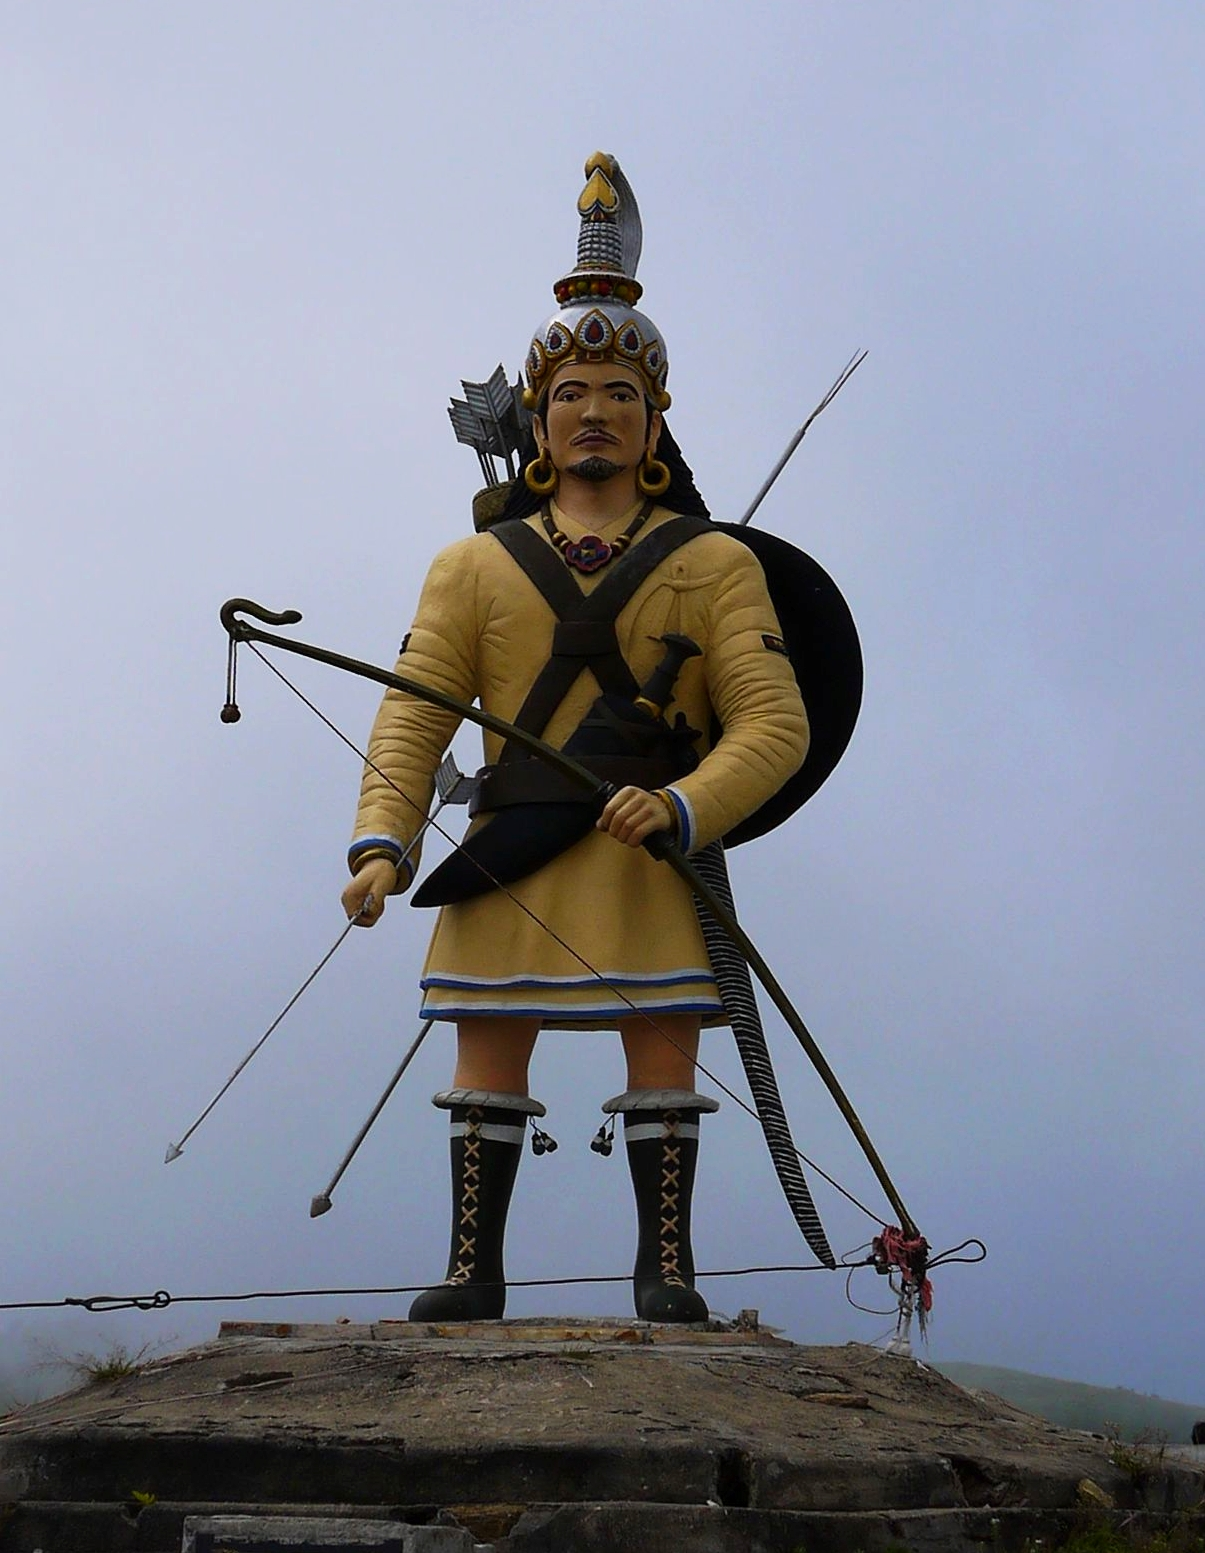
\includegraphics[height=8cm]{figures/yalambar.jpg}
\caption{The statue of the mythical Kiranti king Yalambar in Mudhe Sanischare}\label{yalambar}
\end{figure}


Another iconic figure for Kiranti identity is the 18\textsuperscript{th}-century Limbu scholar Te-ongsi Sirijunga Xin Thebe (Sirijanga) from Sikkim, who is celebrated as the initiator of an ethnic awakening and as the creator of the Limbu script (legendary accounts state that he found and revived the script). He is widely perceived as a martyr for the Kiranti cause, because he was  murdered by the Sikkimese Bhutia rulers, allegedly because they perceived his activities as a threat. He is usually depicted tied to a tree and bristling with arrows, for instance in a statue in Dharan (Tinkune), but also in icon-like prints and posters that can be found in people's homes.


\subsection{The Yakkha}

\subsubsection{Ethnic affiliation}

Within Kiranti, the largest subgroups are the Rai and the Limbu. While the Limbu speak a few very closely related languages, the term Rai is a broad category that subsumes at least 20 linguistically and ethnically distinct communities.  

The Yakkha perceive themselves as closest to the Limbu both culturally and linguistically (see also \citet[90]{Russell1992_Yakha}). Marriages between Yakkha and Limbu are more common than between members of other Kiranti groups. The closest linguistic relative of Yakkha, however, is not Limbu, but the Belhare language, since Yakkha and Belhare share some innovations and unique features that are not found in any other Kiranti language (cf. \sectref{genetic} below). The most likely historical scenario is that the Yakkha have adapted culturally to the Limbu because the latter have been  the economically and socially most powerful group in the region. 

Formerly, the Yakkha were also known as Rai \citep[90]{Russell1992_Yakha}.\footnote{Russell suggests that the name Rai was used when communicating with outsiders to benefit from the reputation of those Rai in the British Gurkha regiments. In present times, too, when talking about my research outside the Yakkha area, I was frequently confronted with the assumption that the Yakkha are a Rai group.}  The Yakkha, however, stress that they neither belong to Rai nor to Limbu. In line with this, it is now popular to use \emph{Yakkha} or one's  clan name as surnames instead of the formerly used exonymic surnames \emph{Dewan} and \emph{Jimi} that originate in Nepali administrative titles given to local tax collectors by the Gorkha kings.\footnote{Cf. \citet[8]{Doornenbal2009A-grammar} for the same observation in Bantawa.} Furthermore,  origin myths that are known from many Rai groups, such as the story about Sumnima and Paruhang or the legends about the orphan hero Khocilipa/Khakculukpa \citep{Ebert2003Camling, Gaenszle2000Origins} are not perceived as native to Yakkha and are not widely known. 

The nature of the historical link to Belhare, which is spoken near Dhankuta, 50 kilometers to the  south of the core Yakkha area, is not known with certainty, but it is worth noting that \citet[13, 47]{Dahal1985An-ethnographic}\footnote{Cited in \citet[1]{Russell1992_Yakha}.} mentions that a group of Yakkha families had been integrated into the Athpahariya (Athpare) society. \citet[21]{Bickel1996Aspect} notes that the people who speak Belhare are also known as Athpare, and that the two linguistic groups Athpare and Belhare are one group  by cultural criteria: their languages are mutually unintelligible, which could be explained by such a migration scenario. This hypothesis is supported by the fact that other Yakkha groups have also out-migrated from the Yakkha homeland (cf. \sectref{geogr}), most probably in search for arable land.


\subsubsection{Language names}

The term \emph{Yakkha} is simultaneously used as a linguistic and as an ethnic name. Alternative names for the language are \emph{Yakkha Ceʔya} (\emph{ceʔya} meaning \rede{matter, talk, language}) and \emph{Jimi Bhasa}, the exonym used by Nepali speakers.  As an ethnonym, the non-indigenous name \emph{Jimi}  is  sometimes used synonymously with Yakkha. It is also a common surname for Yakkha people, introduced during the Gorkha rule. Titles such as \emph{Dewan} and \emph{Jimdar} (from Persian \emph{jamindār}) were given to individuals  and village headmen in the Yakkha area, in order to implement the Gorkha tax system, and they were adopted as surnames because of the power and high social status associated with them. Among the Limbu, the Mughal (Arabic) title \emph{Subba} became a common surname, and among the Khambu, this happened with the title \emph{Rai}  \citep[51]{Whelpton2005A-History}. Apart from these non-indigenous surnames, however, ancestral clan names play a vital role in social life and in the ritual sphere (see \sectref{social} below).  

The first syllable of  \emph{Yakkha} is traceable to the Proto-Kiranti root *\emph{rok}, which is the Kiranti autonym and has no cognates outside Kiranti. Cognates are found e.g. in the Puma autonym \emph{rakoŋ} \citep{Bickeletal2009Puma}, in the Dumi autonym \emph{roʔdi} \citep[413]{Driem1993A-grammar} and in the Limbu autonym \emph{yakthumba} \citep[xix]{Driem1987A-grammar}.  The historical sound change from  /r/ to /y/ is typical for Eastern Kiranti, to which Yakkha and Limbu belong. The neighbouring groups Lohorung, Yamphe and Yamphu  also call their languages \emph{Yakkhaba} \citep[347]{Driem1994The-Yakkha},\footnote{The marker \emph{-ba} has the function of a nominalizer.}  but their languages are clearly distinct from Yakkha.\footnote{A folk etymology relates the language name to the  lexeme \emph{yaksa} \rede{hut, resting place} \citep[87]{Kongren2007Indigenous}. This word is a Tibetan loan (\emph{rgyags-sa})  that is also known in Nepali \citep{Turner1931A-Comparative}.} The second syllable \emph{kha} might be traced back to the Proto-Tibeto-Burman root  *\emph{ka} for \rede{word, speech} \citep[174]{Matisoff2003Handbook}.

   
\subsubsection{Subsistence and economy}
 
The Yakkha are primarily agriculturalists. The main crops are maize (\emph{caloŋ}), rice (\emph{cabhak}), millet (\emph{paŋge}) and  buckwheat (\emph{khoriʔmaŋ}). They also grow soybeans (\emph{cembek/chacek}), lentils (\emph{tuya}), tea (Nepali \emph{ciya}), cucumbers (\emph{wabik}), tomatoes (\emph{wa\-riŋba}), onions (\emph{chepi}), garlic (\emph{maŋkhu}), yams (\emph{khi}), potatoes (\emph{sambakhi}), bananas (\emph{camokla}), Indian leaf mustard (\emph{yaro}), mushrooms (\emph{muŋ}), and various kinds of greens, pumpkins and gourds. A typical household also has pigs, buffalos, oxen, chickens and goats. Pigs and chickens also feature prominently in the ritual design, as a sacrifice to the ancestors. Other means of subsistence are fishing, hunting  and beekeeping.  

The Yakkha press mustard oil (\emph{kiwa}), they brew beer (\emph{cuwa}), mostly from millet, and they distill liquor (\emph{chemha}), also from millet. Alcohol is not just a refreshment, but also a medium of social exchange (e.g. in marriages and fune\-rals) and a sacrifice in the ancestral rituals (see also \citet[124]{Russell1992_Yakha}).  A main source of income is the cultivation and trade of cardamom (mostly called \emph{alenchi}, from Nepali, though the Yakkha term is \emph{cokceru}). Furthermore, various fermented, durable dishes are prepared, most famously \emph{kinama} (fermented soybeans). Traditional agricultural instruments are still used today, because it is impossible to cultivate the terraced fields with machines. Some villages have electric mills to grind the grains, but mostly this is done with grinding stones. According to my observations in Tumok, educated people who have an income as teachers or in other village-level government posts do not necessarily abandon agriculture, but try to maintain both means of subsistence. 

Recruitment in the British Gorkha army has long been a source of income in the Kiranti groups in general. In recent decades, labour migrations to Arab countries, to Hong Kong, Singapore and Malaysia has increased. Most households I got to know in Tumok received some sort of support from family members working abroad. 
%There is a tradition of helping each other by exchanging manpower or animals, known as \emph{parma} in Nepali, which is still occasionally found in the Yakkha context. \citet[216]{Russell1992_Yakha} notes that it has almost disappeared. 


\subsubsection{Material culture}

A typical Yakkha house (\emph{paŋ}) is shown in \figref{house}. Yakkha houses (at least in Tumok) are white, with the lower part of the walls covered in red (a mixture of clay and cowdung). They are typically renovated once a year, before Dasain (the most important Hindu festival in Nepal), although the festival itself is not celebrated in Yakkha society anymore.\footnote{The festival had been celebrated until recently, albeit, as argued by \citet{Russell2004Traditions}, with Yakkha-specific modifications. The recent abandonment of the Dasain festival can be understood as part of a broader process of de-Hinduization among the non-Hindu groups in Nepal. Other Hindu customs prevail, such as the question who may eat together, and who may serve food to whom.} The houses have blue and red wooden railings and window frames, some of them beautifully carved. Every house has a terrace (\emph{omphu}), in which guests are usually received. The roofs are thatched with straw or covered with tiles (or, as a recent development, tin).

\begin{figure}
\centering
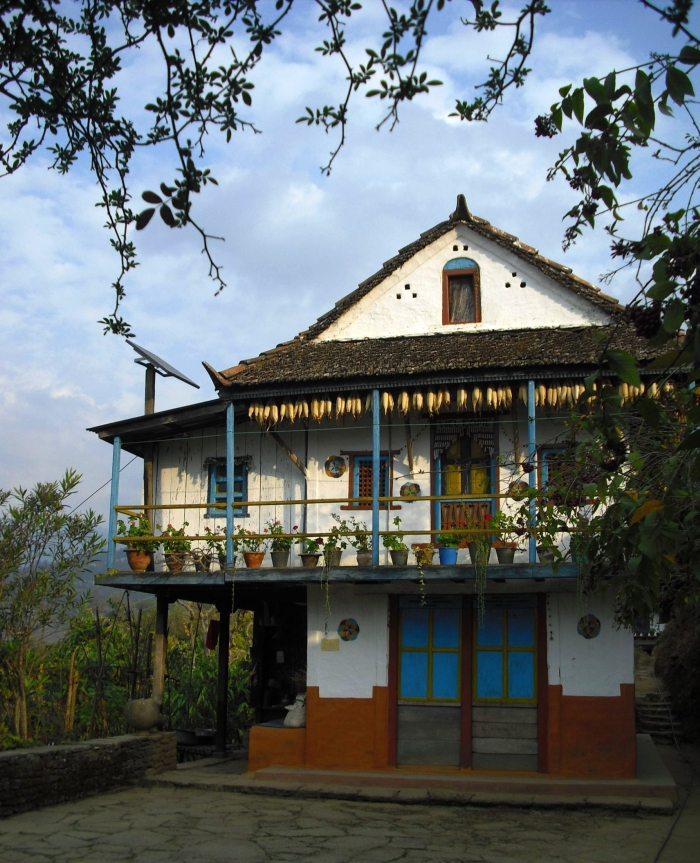
\includegraphics[height=8cm]{figures/house.jpg}
\caption{A Yakkha house in Tumok village}\label{house}
\end{figure}


The Yakkha have a rich tradition of processing bamboo (\emph{phabu}). Bamboo products are abundant in all aspects  of material culture, from house construction to manufacturing various kinds of sieves, baskets and the most delicate and tiny purses, combs and needles, as shown in \figref{phabu}.

Another craft is weaving mats from straw and maize leaves. Furthermore, fabrics and shawls are produced on looms.  The pattern found on traditional Yakkha shawls (\emph{phopma}) is shown in \figref{phopma}. 


 \begin{figure}[h]
 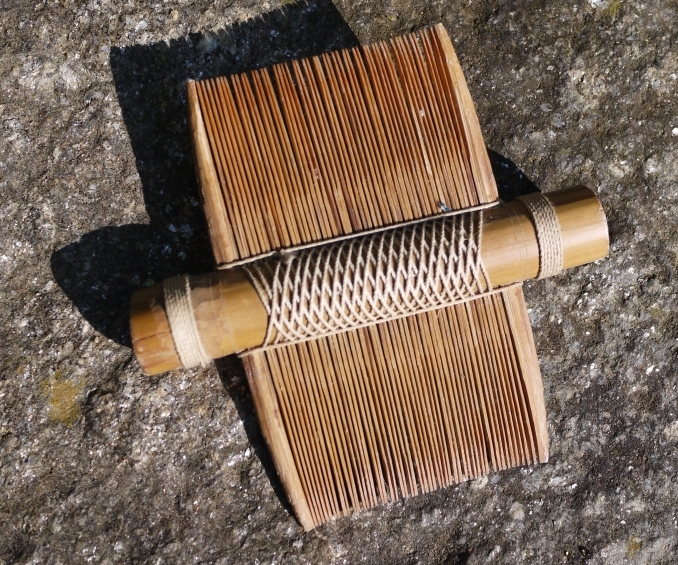
\includegraphics[width=0.30\textwidth]{figures/comb.jpg}
 \hfill
 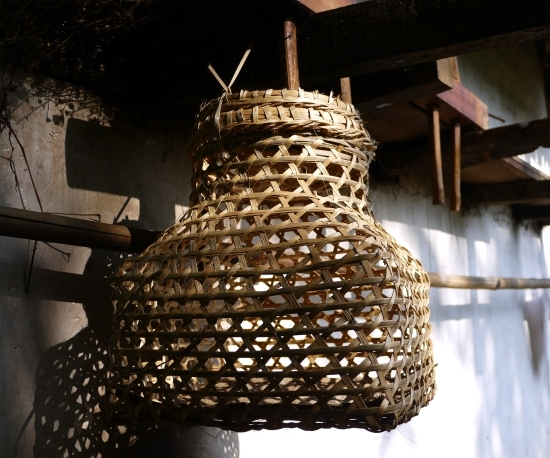
\includegraphics[width=0.30\textwidth]{figures/kangyong.jpg}
 \hfill
 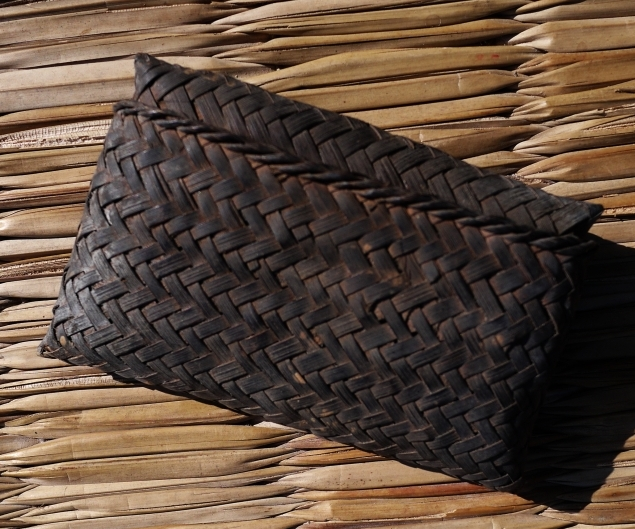
\includegraphics[width=0.30\textwidth]{figures/phepi.jpg}
 \caption{Bamboo  products: \emph{sigikma} \rede{comb}, \emph{kaŋyoŋ} \rede{chicken basket}, \emph{phepi} \rede{purse}}\label{phabu}
 \end{figure}



\begin{figure}[h]
\centering

\includegraphics[height=4cm]{figures/phopma.jpg}
\caption{Yakkha \emph{phopma} (shawl)}\label{phopma}
\end{figure}

\subsubsection{Social organization and religion}\label{social}

The Yakkha religious sphere and social organization are shaped by the pan-Kiranti tradition that is called \emph{munthum} in Yakkha, in which the ancestors play a major role. The term \emph{munthum} also refers to a body of orally transmitted texts in which the deeds and journeys of the ancestors come alive. \citet{Gaenszle_Redefining} notes that, despite differences in ritual systems and practices, this ancestral tradition is shared by  all Kiranti groups. The \emph{munthum}

\begin{quote}
[...] comprises histories of the origin of the ancestors, beginning with the primal creation of the universe and the emergence of natural and cultural orders and continuing to the settlement of the ancestral territory. It also concerns the proper means of communicating with ancestors and ritually maintaining the order they have established. The term, then, has an additional meaning: it evokes a way of life predefined by the ancestors, a self-enclosed world rooted in the past. \citep[224]{Gaenszle2000Origins}
\end{quote}

The social order, but also the physical and mental health of individuals, is ultimately related to the ancestors. This is also illustrated by rituals such as \emph{saya pokma} (literal translation: \rede{raising the head soul}), which is known in Yakkha and in other Kiranti groups. It is undertaken to re-unite individuals, whose well-being is endangered, with the primaeval ancestral order. In her anthropological-psychological study on Lohorung culture, for example, \citet{Hardman2000_Other} notes that the main frame of reference in that culture is one in which

\begin{quote}
... the \rede{natural} ancestral order [...], as recorded in their myths, has to be constantly recreated and the unity between nature, the superhuman, and the human reaffirmed. Failure to do this would lead to depression, increased sickness, possibly death, and ensuing chaos. In contrast, repetition of ancestral worlds and adherence to ancestral order acts like recharging the cosmos. It brings vitality. \citep[12--3]{Hardman2000_Other}
\end{quote}

For  Yakkha people, the ancestral order is equally important. A key feature of this order is the division of the Yakkha society into clans (called \emph{choŋ}), which is critical not only in marriage restrictions but also in the ritual sphere. \citet[201]{Russell1992_Yakha} notes the following clan names in Yakkha (square brackets indicate his transcriptions where deviating from the orthography used in this work): \emph{Linkha}, \emph{Chala} [challa], \emph{Koyoŋwa} [koyoŋa], \emph{Khamyahaŋ} [kammieŋ], \emph{Limbukhim} [limbuhim], \emph{Hoŋhoŋba}, \emph{Koŋgren}, \emph{Choŋgren}, \emph{Maʔkruk}, \emph{Yaʔyukhim}, \emph{Taʔyum}, \emph{Pubaŋgu}, \emph{Oktubaŋ}, \emph{Somyeŋ}, \emph{Khayakhim} [khayakim], \emph{Heŋwa}, \emph{Ilumbaŋ}, \emph{Tiksalaŋ}, \emph{Thampara}, \emph{Ibahaŋ}, \emph{Yuwahaŋ}. I further recorded the clan names \emph{Elaba}, \emph{Hangsewa} and \emph{Huture} in mythical narratives. 

Apart from these clans, there are is another concept called \emph{sametliŋ} \rede{spiritual clan}. There are different  \emph{sametliŋs} for the women and for the men of each clan. Women of one clan may, however, share their spiritual clan with men of another clan. In contrast to clan  (\emph{choŋ}) affinity, the \emph{sametliŋ} of a woman does not change after marriage. The \emph{sametliŋs} outside one's family are not widely known, in contrast to a person's \emph{choŋ}. They are only significant in dealing with spirits (\emph{cyaŋ}) \citep[166]{Russell1992_Yakha}.

Personal names (mostly Indo-Aryan nowadays), are not widely used. It is rather common to adress a person by the respective kinship term, or by a teknonym \rede{X's father} or \rede{X's mother}. 

The ritual specialists responsible for holding the ancestral rituals are called \emph{Maŋgaŋba} in Yakkha. They undertake rituals for each household on occasions like births, marriages and deaths. The task of the \emph{Maŋgaŋbas} is to maintain the ancestral order and good relations with the spirit world (there are several potentially dangerous spirits such as \emph{soghek} - ghosts of people who have died an unnatural death). Other religious practitioners are \emph{chamwas},  \emph{bijuwas} (a Rai term), \emph{phedaŋbas} (a Limbu term), \emph{dhamis} (a Nepali term), but I cannot offer a typology of their features and their tasks. Jointly celebrated festivals (above the clan level or even above the village level) are \emph{casowa} (Nepali: \emph{udhauli}) in late autumn and \emph{yuchyaŋ} (Nepali \emph{ubhauli}) in spring \citep[102ff.]{Kongren2007Indigenous}.\footnote{In his ethnological study, \citet{Russell1992_Yakha}  does not mention these festivals, so their names as well as  celebrating them this way might be a relatively new development.} On these occasions and also on marriages, people gather in a circle and dance a complicated choreography slowly to the sound of huge drums beaten by some men in the circle (\emph{keilakma} \rede{dancing the drum dance}). \todo{Please do not use \emph{ff.}. Please give full page ranges}

The Yakkha society is patrilineal and patrilocal. With regard to marriages, it is important to note that there are two distinct steps taken to incorporate the bride into the clan of her husband. The actual marriage is only the first step, called \emph{mandata}. The second step is called \emph{bagdata}, and is undertaken years, sometimes decades, after the marriage. In the \emph{bagdata}, the husband has to ask his in-laws for their daughter again, and only after this ritual does she become a member of his clan. If the wife dies before the \emph{bagdata} has been asked for, her natal home will undertake the death rites for her.

 
\section{Genealogical affiliation}\label{genetic}

Yakkha is a Sino-Tibetan language, belonging to the Greater Eastern branch of Kiranti, a group of Tibeto-Burman languages spoken in Eastern Nepal.\footnote{Although not  undisputed, it is assumed by many scholars that Sino-Tibetan can be divided into a Sinitic and a Tibeto-Burman branch, the latter containing at least 300 languages \citep{Bradley1997_Tibeto-Burman, Matisoff2003Handbook}.}  Beyond this basic classification, the question of how to group Kiranti languages with other Sino-Tibetan languages is still a controversial issue, as in general, subgrouping in the large and incredibly diverse Sino-Tibetan language family has proven to be rather difficult (see e.g. \citealt[Chapter 3]{Hyslop2011_Kurtop} for an overview of the different models of reconstruction that have been proposed).

\citet{Shafer1974_Introduction} identified Kiranti (which he called East Himalayish) as a sub-branch of Bodic, together with three further branches: Bodish (including Tibetan and Tamangic languages), West Himalayish and West Central Himalayish (including Magar and Chepang). Similarly, \citet{Bradley1997_Tibeto-Burman} suggested that the Kiranti languages, together with Magaric and Newaric languages, form the sub-branch Himalayish. 

A different view is entertained by \citet{LaPolla2003_Overview},  who includes Kiranti in a group he calls Rung (including, most importantly, the rGyalrongic languages, the Dulong languages, the Kiranti languages,  Kham, and the West Himalayan languages Kinauri and Almora), on the basis of shared person marking morphology and a reflexive/middle suffix \emph{*-si} (except for rGyalrong).  What makes any classification even harder is that not even the question of the antiquity of person marking in Tibeto-Burman has been settled yet (see e.g \citet{DeLancey2010_Towards, Jacques2012_Agreement} who argue that such a system can be reconstructed, and \citet{LaPolla2001_Role, LaPolla2012_Comments}, who argues that agreement marking systems in Tibeto-Burman languages are independent innovations).

Kiranti languages can be grouped into a Western and a Central-Eastern branch (with a Central and a Greater Eastern sub-branch), as shown in \figref{fig-Kiranti-tree} (\citealt{Bickeletal_Firstperson}). Central-Eastern Kiranti is characterized by a loss of voiced initials by merging voiceless and voiced initials \citep{Michailovsky1994Manner}. Voiced stops with phonemic value rarely occur, though voiced allophones are possible, as a result of post-nasal and intervocalic voicing, for instance in Yakkha and in Athpare \citep[505]{Ebert2003Kiranti}. 

\todo{Maybe a TikZ-picture would be better suited here than qtree using node and child node. Right now, this tree is hardly readable and I would like to enlarge it. However I have not found a way to manually set vertical distances in qtree which is necessary here in order to scale this tree correctly. I think tikZ can do this. }

	\begin{figure}[h]
	\resizebox{\textwidth}{!}{
		\setlength{\qtreepadding}{2pt}
		\setlength{\abovecaptionskip}{10pt}

		{\scriptsize
		\Tree 
		[.\fbox{\textbf{Kiranti} }
			[
				[.{Western\\(*ʔC → C)} 
				{Chaurasiya\\(*ch → s):\\Jero\\Wambule} 
				{Northwestern:\\Bahing/Bayung\\Hayu\\Sunuwar/Koĩc} 
				{Upper Dūḍhkośī:\\Khaling\\Dumi} 
				] 
				[.{Midwestern\\(*ʔp,*ʔt → b,d):\\Thulung\\Koyu}
				] !\qsetw{-2cm}
			]
			[.{\fbox{\textbf{Central-Eastern}}\\(*voiced → voiceless;\\*ʔk,*ʔc → kh, ch)} 
				[.{Central\\(*ʔp,*ʔt → b,d)} 
					{Khambu\\(*ʀ→ g, hr):\\Kulung\\Nachiring\\Sampang\\Sam} 
					{Southern:\\Camling\\Bantawa\\?Dungmali\\Puma} 
				] 
				[.{\fbox{\textbf{Greater Eastern}}\\ (*ʔp,*ʔt → ph, th)} 
					{Upper Aruṇ\\(PE *ph,*th → $\emptyset$):\\Lohorung\\Yamphu\\Mewahang}  
					!\qsetw{1cm} [.{Eastern\\(ʀ,r → y)} 
						{\fbox{\textbf{Greater Yakkha}}:\\\fbox{\textbf{Yakkha}}\\?Mugali\\Ch\textbari l\textbari ng\\Chintang\\Athpare\\Belhare (PE *th → $\emptyset$)} 
						{Limbu\\(ch → s)} 
					] 
				] 
			] 
		]
		}
	}
	\caption{Kiranti subgrouping, according to \cite{Bickel2008Seminar}}\label{fig-Kiranti-tree}
	\end{figure}
	
 
Yakkha undoubtedly belongs to the Greater Eastern branch. A distinctive feature of Greater Eastern Kiranti languages is the change of pre-glottalized stops into aspirated stops  (or zero, in the case of /*ʔt/, see further below):  */ʔts/ > /tsʰ/, */ʔp/ > /ph/,  */ʔk/ > /kh/ (see \tabref{soundchange} for comparative data).\footnote{The table is based on data from \citet{Driem1993A-grammar, Driem1987A-grammar, Bickeletal2009Puma, Kongren2007Yakkha} and my own data.} The Greater Eastern branch splits into Upper Arun (Lohorung, Yamphu and Mewahang) and Eastern Kiranti, to which Yakkha belongs. Eastern Kiranti is characterized by  the change of  initial */r/ and */R/ into /y/ \citep{Driem1990The-fall}.

Within Eastern Kiranti there are two groups, which are the various Limbu dialects on the one hand and the so-called Greater Yakkha group, with Chintang, Belhare, Athpare,  Chɨlɨng and Yakkha, on the other hand. Some languages of the Greater Yakkha branch are characterized by the loss of the aspirated coronal stop, compare e.g. Limbu \emph{thuŋ} \rede{drink} with Yakkha (and Belhare) \emph{uŋ} \citep{Bickel1997Dictionary}. Furthermore, the aspirated affricate /tsʰ/ (see above) has undergone a further change to /s/ in Limbu, compare e.g. Limbu \emph{sarumma} with Yakkha \emph{chalumma} \rede{second-born girl} (for further examples see \tabref{soundchange}). 

Rhotic consonants, although they do  not occur word-initially  in Yakkha, are found word-internally. The claim made by  \citet{Driem1990The-fall} that [l] and [r] have a complementary distribution and are thus allophones in Eastern Kiranti cannot be confirmed for Yakkha: both sounds occur in similar environments word-internally  (cf.  \tabref{r-l} on page \pageref{r-l}), and no environment was found  in which [l] and [r] show allophonic variation  in Yakkha  (see also \sectref{rhotic}). Thus, although finding “proper” minimal pairs for /l/ and /r/ is difficult, /r/ is a phoneme in Yakkha.

\begin{table}[t]
{\small
\begin{tabular}{llllll}
\lsptoprule
{\sc Proto-}&  {\sc Dumi}  &  	{\sc Puma} &  {\sc Yakkha} &  {\sc Limbu} &  \\
 {\sc Kiranti }  &   ({\sc western}) &  ({\sc central}) &  ({\sc eastern}) &   ({\sc eastern}) &{\sc gloss} \\
\midrule
\char"002A /d/		& 	deːn	&  		ten 		&  	ten	&  tɛn	& 	\rede{village}	 \\
\char"002A /j/		& 	ju&  ca&  ca &  ca&  \rede{eat}	 \\
\char"002A /b/		& 	bhiʔi&  pooŋ&  pik &  pit & 	 \rede{cow} \\
\char"002A /r/		&  rep	&  rep &  ep&  yep & 	  \rede{stand}\\
\char"002A /r/		&  roʔdi	&  roduŋ&  yakthuŋ&  yak & 	  \rede{Kiranti} (autonym)\\
\char"002A /R/		&  r\textbari m	&  rum&  yum&  yum& 	 \rede{salt} \\
\char"002A /ch/		&   	&  chapd-&  chep & sap   & 	 \rede{write} \\
\char"002A /ʔc/		&  	&  chakd &  chekt &  sak& 	 \rede{close} \\
\char"002A /ʔp/		&  puŋ	&  buŋ &  phuŋ &  phuŋ& 	 \rede{flower} \\
\char"002A /ʔt/		& 	t\textbari ŋ&  duŋ&  uŋ&  thuŋ& 	 \rede{drink} \\
\char"002A /ʔt/		& 	&  dok &  ak & thak & 	 \rede{loom} \\
\lspbottomrule
\end{tabular}
}
\caption{Examples of Kiranti sound correspondences}\label{soundchange}

\end{table}

Based on a comparison of the verbal person marking paradigm, the closest re\-lative of Yakkha within the Greater Yakkha branch is Belhare. The two languages exclusively share the following markers: a suffix \emph{-ka \ti -ga} indexing second person arguments (any role), and an underspecified nasal prefix \emph{N-} indexing third person plural S and A (3>2.{\sc sg} and 3pl>3) in Yakkha, and  3nsg.S and 3>2 in Belhare \citep[551]{Bickel2003Belhare}. 



\section{Sociolinguistic context}\label{socioling}
\subsection{Dialectal variation}\label{sc-dialect}

The variety documented here is spoken in Tumok village and surrounding areas, e.g. in Salle. No detailed dialectal study has been undertaken for Yakkha yet. Based on phonological differences and distinct exclamative words, I tentatively propose three further dialects: one spoken in the area around Ankhinbhuin (Angbura, Hombong, Phakling), one spoken in the area around Dandagaun and one spoken towards the north, in Kingring and Kharang villages. 

\tabref{dialects} illustrates dialectal differences. The Kharang dialect is different from the other dialects, for instance, in having a second person possessive marker \emph{i-} instead of the unspecified nasal prefix that is found elsewhere,  and in having a clause-final exclamative particle \emph{ikhok}. Apart from this, I do not have data on this dialect. 

Yakkha has a general phonological rule of voicing consonants in post-nasal and intervocalic position. The rule has different domains of application across the dialects: in Tumok and in Dandagaun it does not apply to aspirated consonants, while in Ankhinbhuin it applies to both aspirated and unaspirated consonants. Furthermore, I noticed that in Dandagaun,  /o/ gets raised to /u/, at least in some lexemes. In the Tumok  dialect, the person marker for first person acting on second is \emph{-nen}, while in the Ankhinbhuin dialect it is \emph{-nan} (cf. also the data from Omruwa (Angbura) in \citealt{Driem1994The-Yakkha}). In Dandagaun and Ankhinbhuin honorific imperative forms calqued upon Nepali are used, while in  this is not common in Tumok. I have no data on the varieties spoken in the south of the Dhankuta district, in the village of Namsaling in Ilam district and in India.


\begin{table}
\centering
\begin{tabular}{lllll}
\lsptoprule
{\sc tumok}	&	{\sc dandagaun}	&{\sc ankhinbhuin}	&	{\sc kharang}&	{\sc gloss}\\
\midrule
\emph{mma}	&\emph{mma}	&\emph{mma}	&\emph{ima}		&\rede{your mother}\\
\emph{nniŋga}	&\emph{nniŋga}	&\emph{nniŋga}		&	\emph{iniŋga}	&\rede{your}\\
\emph{i \ti ina \ti iha}	&\emph{i \ti ina \ti iha}&\emph{i \ti ina \ti iha}		&	\emph{iruk}	&\rede{what}\\
\emph{cokma}&\emph{cukma}	&\emph{cokma}			&	(no data)	&\rede{do, make}\\	
\emph{ŋkhya(ci)}&\emph{ŋkhya(ci)}&\emph{ŋghya(ci)}&		(no data)	&\rede{they went}\\	
\emph{mphopma}&\emph{mphopma}	&\emph{mbhopma}			&	(no data)	&\rede{your shawl}\\
\emph{piʔnenna}	&\emph{piʔnenna}	&\emph{piʔnanna}	&	(no data)	&	\rede{I gave it to you}\\
\emph{coeba}	&\emph{cama leŋniba}	&\emph{cama leŋniba}&	(no data)	&\rede{Please eat.}\\
\emph{haʔlo}	&	(no data)	&\emph{khoʔo \ti kho}&\emph{ikhok}&(exclamative particle)\\
\emph{=pa}	&			\emph{=pa}	&\emph{=aŋ}&	(no data) &(emphatic particle)\\
\lspbottomrule
\end{tabular}
\caption{Dialectal variation within the Yakkha region}\label{dialects}
\end{table}



In Marek \textsc{vdc} in Dhankuta (Marek, Ghorlikharka, Jitpur, Andrung, Magwa, Saldang villages),  a variety is spoken that is so different from the other Yakkha varieties (as perceived by  the speakers of Yakkha, too) that it cannot be called a dialect of Yakkha any more. The linguistic differences notwithstanding, the speakers are perceived as belonging to the Yakkha group on ethnic grounds. The language is called Lumba-Yakkha in the Ethnologue (ISO 639-3: luu).\footnote{\citet{Levisetal2015_Ethnologue}, http://www.ethnologue.com, accessed on Dec. 20 2013} I have not heard this designation in Tumok, the language was usually referred to as \emph{māreki bhāsā} (Nepali; \rede{the language from Marek}). The Marek variety has, for instance, undergone the sound change from /ch/ to /s/ that is also known from Limbu. Crucially, the pronominal paradigm and the verbal inflection are different from Yakkha, for instance the second person prefix \emph{a-}  (otherwise known from Athpare and Chintang, see \citealt{Ebert1997A-grammar, Bickeletal2007Free}) instead of the Yakkha suffix \emph{-ka}. \tabref{lumba} provides some exemplary data collected in 2010 with a speaker from Marek, but no detailed study has been undertaken yet. 

\begin{table}
\centering
\begin{tabular}{lll}
\lsptoprule
{\sc marek}&	{\sc tumok}	&		{\sc gloss}\\
\midrule
\emph{hoʔli}&\emph{imin}&\rede{how}\\
\emph{pisa}&\emph{picha}&\rede{child}\\
\emph{seŋma}&\emph{chimma}&\rede{to ask}\\
\emph{hima}&\emph{i \ti ina \ti iha}&\rede{what}\\
\emph{mahuma}&\emph{maghyam}&\rede{old woman}\\
\emph{pahuba}&\emph{paghyam}&\rede{old man}\\
\emph{nhandi}&\emph{khaʔla}&\rede{like this}\\
\emph{aŋga}&\emph{ka}&\rede{I}\\
\emph{aŋciŋ}&\emph{kanciŋ}&\rede{we} (du)\\
\emph{aŋniŋ}&\emph{kaniŋ}&\rede{we} (pl)\\
\emph{ŋkhan}&\emph{nda}&\rede{you} (sg)\\
\emph{habe}&\emph{heʔne}&\rede{where}\\
\emph{hannalam}&\emph{heʔnhaŋ}&\rede{where from}\\
\emph{akhaʔneʔna}&\emph{khemekana}&\rede{you go}\\
\emph{=na}&\emph{=na}&(nominalizer)\\
\emph{-ma}&\emph{-ma}&(infinitive marker)\\
\lspbottomrule
\end{tabular}
\caption{Marek data in comparison with Tumok data}\label{lumba}
\end{table}

\subsection{Endangerment}\label{endangerment}

According to the Nepali census of 2001 \citep{\textsc{cbs}2001Report} and the UNESCO Working Paper No. 7 \citep{Toba2005Unesco}  there are 14,648 native speakers out of about 17,000 ethnic Yakkha. The number of native speakers makes up 0.06 per cent of the Nepalese population. This census, however, seems highly optimistic to me, since Yakkha is barely spoken in half of the Yakkha area, and even where it is spoken the youngest generation (below 20 years of age) does not commonly use Yakkha, even though they might have a passive command of the language. Specific domains such as ritual, mythological and traditional ecological knowledge are known only by a few (usually) elderly people. I did not find any monolingual Yakkha speakers; all speakers are at least bilingual with Nepali,\footnote{The official language in Nepal is the Indo-Aryan language Nepali. It is used in official communication,  in commerce and in  education. Since the constitution of 1990 which followed the first \emph{Jana Andolan} (People's uprising), all languages spoken as mother tongues in Nepal are considered national languages, which grants the speakers the right to be educated in their mother tongue \citep{Turin2007_Diversity}. This is, however, hard to implement, given that more than 100 languages are spoken in the country.} and proficiency in other neighbouring languages such as Bantawa and Limbu is also common.

One reason why Yakkha  speakers shift to Nepali is the already mentioned migration outward for economic and educational reasons, but there are also whole  villages inside the  homeland that have switched to Nepali. For instance, while Yakkha is still vividly spoken in Tumok, it is difficult to find speakers in the neighbouring villages Mamling, Waleng and in the old garrison town Chainpur (a former center for trade in the region). Most speakers of Yakkha are found in the south of the Yakkha region.

A well-known reason for this development is the low prestige that indigenous languages have long  had compared to Nepali. Since the creation of the Nepali nation state in the eighteenth century under the rule of King Pr̥thvī Nārāyaṇ Śāha (1723–1775), Nepali has been propagated as the national language, and people have  not been encouraged to speak other languages. Much damage was also done under the Panchayat System (1961–1990), where the use of indigenous languages was actively discouraged under the policy of “One Nation, One Language” \citep[20]{Toba2005Unesco}.

Language shift is complex and can be understood on both macro and interactional levels of analysis. In the Yakkha region, education beyond the primary school level is available exclusively in Nepali or English.\footnote{This is also reflected in the negative correlation between the educational level and the number of Yakkha students. According to the 2001 census, the number of Yakkha students beyond the primary level was 6915, the number of those who have passed \textsc{s.l.c} was 878 and the number of those with a degree was 89 in 2001 \citep{\textsc{cbs}2001Report}.} At the primary level, Yakkha language classes have been introduced in a number of schools recently (starting in 2009), but Yakkha is not the medium of instruction in other subjects. Yakkha people are not represented in the government beyond village level \citep{\textsc{cbs}2001Report}. Even in the villages, official posts in education and administration are still overwhelmingly held by people from  non-indigenous backgrounds, simply because there are not enough Yakkha people who could work in these positions. This social and economic bias exerts additional pressure on the speakers of Yakkha, and these dynamics are one of the reasons why Yakkha-speaking parents use Nepali with their kids. 


Another factor destabilizing the language situation are marriages with people outside one's  own linguistic community, for instance Yakkha-Limbu marriages. Generally, bilingual or multilingual families are of course not problematic, to the contrary, multilingualism is rather the norm world-wide (see \citealt{Turin2007_Diversity}). But with the additional pressure that comes from Nepali, children from multilingual families nowadays often grow up with Nepali as the only language they speak fluently. 

These developments cannot simply be related to a lack of interest in the parents to pass on their language. According to my own observations, the tendency not to speak Yakkha is even present in the children of those people who have a high ethnic awareness and who are engaged in a number of activities towards preserving their language and culture. The tension between preserving one's  ethnic and linguistic heritage and participating in modern society is well-known in theoretical approaches to language loss, but it is nevertheless hard to resolve for the affected individuals.

In the past decades, with multi-party democracy having started in 1990, and even more so in the post-monarchy era that has followed the civil war (1996–2006) and the second \emph{Jana Andolan} (People's Uprising) in 2006, activities aiming at the preservation of the indigenous languages and cultures have increased. In the case of Yakkha, for instance, the Kirant Yakkha Chumma (Indigenous Peoples Yakkha Organization) have implemented Yakkha lessons in a few primary schools in the Yakkha region.  School books have been completed up to class five already, with the plan to reach class eight. Dictionaries, literary works and even songs and music videos have been created lately by members of the community who feel the urge to do something before it is too late (cf. \sectref{earlier-work}). The long-term impact of this welcome development remains to be seen. To properly assess the endangerment of a language, an in-depth study in its own right would be necessary. The loss of Yakkha in a wide geographic area and in the youngest generation are, however, very clear and alarming signs.






 %%\input{chapters/03_Typological_Profile.tex}
 \chapter{Phonology}\label{phon}


This chapter deals with the phoneme inventory and phonological  and morpho\-phonological rules and processes that are relevant in Yakkha. The orthography used here is explained  in \sectref{orth}. The examples in this chapter, unlike in the other chapters, have two lines representing the Yakkha data: the upper line shows the data after the application of all phonological and morphophonological rules, and the lower line shows the underlying phonemic material with morpheme breaks. The orthography is used in both of these representations, and \textsc{ipa} is only used when it is necessary in the explanations in prose. \sectref{phon-inv} presents the phoneme inventory of Yakkha,   \sectref{syllable} treats the syllable structure and  \sectref{loansphon} discusses the treatment of loan words, as they nicely illustrate the phonological features of Yakkha. \sectref{stress} lays out the conditions by which stress is assigned. The abundant morphophonological processes and their connections to syllable structure, stress and to diachronic processes are the concern of \sectref{morphophon}. 


\section{Phoneme inventory and allophonic rules}\label{phon-inv}

\subsection{Vowel phonemes}\label{vowelphon}

Yakkha has only five basic vowels; it has two close vowels, the front /i/ and the back /u/, two close-mid vowels, the front /e/ and the back /o/, and an open vowel /a/. In contrast to other Kiranti languages,  there are no central vowels like  /ɨ/, /ʌ/ or /ə/. A chart with the vowel inventory is provided in \figref{fig-vowels}. In addition to these vowels, a  front vowel [ɛ] may occur, but only as the  contracted form of the diphthong /ai/ (see \sectref{diphth}), not in any other environments. Minimal pairs are provided in \tabref{min-pair-v}. Tone, length or nasal articulation do not constitute phonemic contrasts in Yakkha. 

\begin{center}
\begin{figure}
	\begin{tikzpicture}[scale=1]
		\node (a3) at (0, 0) {u};
		\node (a1) at (-4, 0) {i};
		\node (a2) at (-2, 0) {};

		\node (b1) at (-3.4,-1) {e};
		\node (b2) at (-1.7,-1) {};
		\node (b3) at (0,-1) {o};

		\node (c1) at (-2.8,-2) {};
		\node (c2) at (-1.4,-2) {};
		\node (c3) at (0,-2) {};

		\node (d1) at (-2.2,-3) {a};
		\node (d2) at (-1.1,-3) {};
		\node (d3) at (0,-3) {};
		
		 \draw (a1) -- (a2) -- (a3);
		\draw (b1)--(b2)--(b3);
		\draw (c1)--(c2)--(c3);
		\draw (d1)--(d2)--(d3);
		
		\draw (a1)--(b1)--(c1)--(d1);
		\draw (a2)--(b2)--(c2)--(d2);
		\draw (a3)--(b3)--(c3)--(d3);
	\end{tikzpicture}

   \caption{Yakkha vowel phonemes}\label{fig-vowels}
 \end{figure}
\end{center}


 \begin{table}[htp]	
 \begin{center}		
\begin{tabular}{lllll}
\lsptoprule
{\sc phonemes}	& \multicolumn{4}{c}{{\sc examples}}\\
\midrule
{\bf /e/ vs. /i/} & \emph{nema} & \rede{lay, sow seed} &\emph{nima} & \rede{know, see}\\
			& \emph{tema} & \rede{lean on an angle} & \emph{tima} & \rede{put down, invest}\\
{\bf /e/ vs. /a/} &\emph{tema} & \rede{lean on an angle} &  \emph{tama} & \rede{come}\\
			&\emph{yepma} & \rede{stand} &  \emph{yapma} & \rede{be rough, uncomfortable}\\
{\bf /o/ vs. /u/} & \emph{okma} & \rede{shriek} &  \emph{ukma} & \rede{bring down}\\
			& \emph{hoʔma} & \rede{prick, pierce} &   \emph{huʔma} & \rede{push, stuff}\\
{\bf /o/ vs. /a/} & \emph{thokma} & \rede{spit} &   \emph{thakma} & \rede{weigh, hand up, send up}\\
			& \emph{hoʔma} & \rede{prick, pierce} &  \emph{haʔma} & \rede{scrape off/out}\\
{\bf /u/ vs. /i/} & \emph{ukma} & \rede{bring down} &   \emph{ikma} & \rede{chase}\\
			& \emph{umma} & \rede{pull} &   \emph{imma} & \rede{sleep}\\
\lspbottomrule
\end{tabular}
\caption{Minimal pairs for vowel phonemes}\label{min-pair-v}
\end{center}
\end{table}


\subsection{Diphthongs}\label{diphth}

Given that adjacent vowels are generally avoided in Yakkha, it does not come as a surprise that diphthongs, i.e., adjacent vowels in the same syllable, are rare. The four diphthongs /ai/, /ui/, /oi/ and /au/ were found, occuring marginally, as in \emph{ŋhai} (a dish made from fish stomach), \emph{hoi!} \rede{enough!},  \emph{uimalaŋ} \rede{steeply downhill}, \emph{(h)au} (a sentence-final exclamative particle) and \emph{ambau!} (an exclamative  expression indicating that the speaker is impressed by huge or dangerous things). Some speakers pronounce underlying sequences like /ŋond-siʔ-ma/ and /thend-siʔ-ma/ with nasalized diphthongs, [ŋoĩsiʔma] and [theĩsiʔma], respectively (instead of the more common pronunciations [ŋonsiʔma] and [thensiʔma]).\footnote{The nasalization is exceptional here. Usually, the prosody of Yakkha supports the opposite process, namely the change of nasal vowels to nasal consonants, e.g. in borrowed Nepali lexemes (see \sectref{loansphon}). Nasals may, however, regularly change to nasalization of the preceding vowel in intervocalic environment and before glides and liquids, as in \emph{mẽ.u.le} \rede{without entering} (/meN-us-le/) and \emph{mẽ.yok.le} \rede{without searching} (/meN-yok-le/), see \sectref{nas-son}.} 

Most diphthongs have their origin in a multimorphemic or in a multisyllabic environment. The adverb \emph{uimalaŋ}, for instance, like many other spatial adverbs in Yakkha, is composed of a stem (diachronically most probably a noun) and the possessive prefix \emph{u-}. The marginal nature of the diphthongs is confirmed also by the fact  that they are found more in names and discourse particles than in lexemes with semantic content, and never in verbal roots. Occasionally, diphthongs are just one stage in a larger process of contraction. Consider the inflected form \emph{waiʔ.na} \rede{(he/she/it) exists}, which is also found as [wɛʔ.na]. Its nonpast semantics and synchronically available contracted forms of verbs suggest that [waiʔ.na]  used to be *\emph{[wa.me.na] } historically. \tabref{table-diphth} provides an exhaustive list of lexemes containing diphthongs from the more than 2400 lexemes in the current lexical database.



 \begin{table}[htp]	
 \begin{center}		
\begin{tabular}{llll}
\lsptoprule
{\bf /au/}&{\bf /oi/}&{\bf /ui/}&{\bf /ai/}\\
\midrule
\emph{(h)au}&\emph{coilikha}&\emph{uimalaŋ}&\emph{ŋhai}\\
({\sc excla})&(a village)&\rede{steeply downhill}&\rede{fish stomach}\\
\emph{ambau!}&\emph{hoiǃ}&\emph{phakkui}&\emph{Yaiten}\\
\rede{holy smoke!}&\rede{enoughǃ}&\rede{pig droppings}&(a village)\\
  & &\emph{waghui} &\emph{lai}\\
 & & \rede{chicken droppings}&({\sc excla})\\
\lspbottomrule
\end{tabular}
\caption{Lexemes containing diphthongs}\label{table-diphth}
\end{center}
\end{table}


\subsection{Consonant phonemes}\label{consphon}

\tabref{fig-consonants} below shows the central and the marginal consonant phonemes of Yakkha. The phones that are not in parentheses clearly have phonemic status; they occur in basic, uninflected stems. The phonemic status of the phones in parentheses is not always straightforward (discussed below). Where my orthography deviates from \textsc{ipa}, this is indicated by angle brackets.

\begin{table}[htp]
\begin{centering}
{\small
\begin{tabular}{lcccccc}
\lsptoprule
			& {\sc bilabial} &	{\sc alveolar} &	{\sc retroflex }	&	{\sc palatal }&	{\sc velar }&		{\sc glottal}\\
\midrule
{\sc Plosives		}& p   	&	t   	&	(ʈ)  	&			&	k   	& ʔ\\
 {\sc asp.}		& ph   &	th  	&	 (ʈh) 	&			&	kh 		&\\

{\sc voiced}& (b)  	&	(d)   	&	 (ɖ) 	&			&	(g)   	&\\
 {\sc voiced-asp.	}	& (bh)   &	(dh)  	&	  (ɖh)	&			&	(gh) 	&\\

{\sc Affricates 	}&		&	ts <c>		&	  	&		 	&			&	\\
{\sc asp.} 	&		&	tsʰ <ch>		&	 	&	  	&			&\\
{\sc  voiced}	&		&	(dz)	 <j>	&	  	&	 &			&	\\
{\sc voiced-asp.} 	&		&	(dzʰ) <jh>		&	 	&	   	&			&\\

{\sc Fricatives }	&		&	 		s&		&		 	&		 	& h	\\
{\sc Nasals	}	&	m 	&	n		&		&			&		ŋ	&	\\
{\sc Nas. asp.}		&	(mh)	&	(nh)		&		&			&		(ŋh)	&	\\
{\sc Rhotics 	}&		&			r&		 &			&			&	\\
{\sc Laterals	}&		&			l&		 &			&			&  	\\
{\sc Glides 	}	& w		&			&		&y			&		 	&	\\
{\sc Glides asp.} & wh	&			&		&			&			&\\
\lspbottomrule
\end{tabular}\\
}
\caption{Yakkha consonant phonemes}\label{fig-consonants}
\end{centering}
\end{table}


\subsubsection{The main phonemic distinctions in the consonants}


Yakkha distinguishes six places of articulation: bilabial, alveolar, retroflex (or post-alveolar), palatal, velar and glottal. Retroflex plosives most probably made their way into Yakkha via Nepali loan words. They are found only in a few Yakkha lexemes, and no proper minimal pairs could be established. The retroflex series lacks a nasal, too. However, in the few words that are found with retroflex stops, they are robust, and pronouncing these words with an alveolar stop is not an option. 

Yakkha fits well into the Eastern branch of Kiranti, for instance in the loss of phonemic  contrast between voiced and unvoiced plosives. Generally, plosives, unless they are found in an environment that triggers voicing, are pronounced voiceless. As always, a few exceptions occur that cannot be explained by some rule. The exact parameters of the voicing rule are laid out in  \sectref{voicing}. A robust phonemic contrast is that between aspirated and unaspirated consonants, found in the plosives (except for the glottal stop), the affricate and the bilabial glide /w/. Aspiration of a stem-initial consonant, historically a morphological means to increase the transitivity in Tibeto-Burman \citep{Michailovsky1994Manner, Jacques2012_Internal, Hill2014_Note}, has become purely phonemic in Yakkha.  The aspirated plosives have a strong fricative component. Three nasals are distinguished by their place of articulation: bilabial  /m/, alveolar /n/ and velar /ŋ/. Yakkha has two fricatives /s/ and /h/, and two liquids, /l/ and /r/. The rhotic does not occur word-initially. In this position, */r/ has changed to the palatal glide /y/ (see also  \tabref{soundchange} in Chapter \ref{languageintro} and the references therein).\footnote{Furthermore, /y/ may be omitted before /e/ in some lexemes, but this process is subject to considerable individual variation.}  The distribution of the rhotic consonant deserves a closer look, also in the perspective of other Eastern Kiranti languages (see \sectref{rhotic} below). \tabref{min-pair-c} provides minimal pairs for the basic consonant phonemes, mostly from verbal stems or citation forms.


 \begin{table}[htp]
\begin{center}
\begin{tabular}{lllll}
\lsptoprule
{\sc phonemes}	& \multicolumn{4}{c}{{\sc examples}}\\
\midrule
{\bf /k/} vs. {\bf /kh/} & \emph{keʔma} & \rede{come up} & \emph{kheʔma} & \rede{go}\\
			& \emph{kapma} & \rede{carry along, have} & \emph{khapma} & \rede{thatch, cover}\\
{\bf /p/} vs. {\bf /ph/} & \emph{pakna} & \rede{young guy} & \emph{phak} & \rede{pig}\\
		 & \emph{pekma} & \rede{fold} & \emph{phekma} & \rede{slap, sweep}\\
{\bf /t/} vs. {\bf /th/} & \emph{tumma} & \rede{understand} & \emph{thumma} & \rede{tie}\\
 		 & \emph{tokma} & \rede{get} & \emph{thokma} & \rede{hit with horns}\\	
{\bf /c/} vs. {\bf /ch/} & \emph{cikma} & \rede{age, ripen} & \emph{chikma} & \rede{measure, pluck}\\
 		 & \emph{cimma} & \rede{teach} & \emph{chimma} & \rede{ask}\\
{\bf /k/} vs. {\bf /ʔ/} & \emph{okma} & \rede{shriek} & \emph{oʔma} & \rede{be visible}\\
 {\bf /t/} vs. {\bf /ʔ/ }& \emph{-met} & ({\sc caus}) & \emph{-meʔ} & ({\sc npst})\\
 {\bf /p/} vs. {\bf /ʔ/} & \emph{opma} & \rede{consume slowly} & \emph{oʔma} & \rede{be visible}\\
{\bf /t/} vs. {\bf /r/ }& \emph{ot} & \rede{be visible} (stem) & \emph{or} & \rede{peel off}\\
 {\bf /l/} vs. {\bf /r/} & \emph{khelek} & \rede{ant} & \emph{kherek} & \rede{hither}\\
 {\bf /y/} vs. {\bf /w/} & \emph{yapma} & \rede{be uncomfortable} & \emph{wapma} & \rede{paw, scrabble}\\
 		 & \emph{yamma} & \rede{disturb} & \emph{wamma} & \rede{attack, pounce}\\
{\bf /y/} vs. {\bf /l/} & \emph{yapma} & \rede{be uncomfortable} & \emph{lapma} & \rede{accuse, blame}\\
 {\bf /w/} vs. {\bf /wh/ }& \emph{wapma} & \rede{paw, scrabble} & \emph{whapma} & \rede{wash clothes}\\
 		 & \emph{waŋma} & \rede{curve, bend} & \emph{whaŋma} & \rede{boil}\\
{\bf /s/} vs. {\bf /h/}& \emph{sima} & \rede{die} & \emph{hima} & \rede{spread}\\
		& \emph{somma} & \rede{stroke gently} & \emph{homma} & \rede{fit into}\\
{\bf /k/} vs. {\bf /ŋ/}& \emph{pekma} & \rede{break} & \emph{peŋma} & \rede{peel}\\
 		 & \emph{okma} & \rede{shriek} & \emph{oŋma} & \rede{attack}\\
{\bf /ŋ/} vs. {\bf /m/} & \emph{toŋma} & \rede{agree} & \emph{tomma} & \rede{place vertically}\\
			 & \emph{tuŋma} & \rede{pour} & \emph{tumma} & \rede{understand}\\
{\bf  /ŋ/} vs. {\bf /n/} & \emph{=ŋa} & ({\sc erg}) & \emph{=na} & ({\sc nmlz.sg})\\
{\bf /m/} vs. {\bf /n/} & \emph{makma} & \rede{burn} & \emph{nakma} & \rede{beg, ask}\\
& \emph{miʔma} & \rede{think, remember} & \emph{niʔma} & \rede{count, consider}\\
\lspbottomrule
\end{tabular}
\caption{Minimal pairs for consonants}\label{min-pair-c}
\end{center}
\end{table}



\subsubsection{Marginal consonant phonemes}

Several of the phonemes occur only marginally,  either in Nepali loan words, or in just a handful of Yakkha lexemes. This basically applies to the already mentioned retroflex plosives and to all voiced obstruents, as voicing is generally not distinctive in Yakkha.\footnote{There are quasi minimal pairs such as \emph{apaŋ} \rede{my house} and \emph{abaŋ} \rede{I came}, but both are inflected words and the difference is that \emph{a-} in \emph{apaŋ} is a prefix, and the rule that is responsible for the voicing of plosives excludes prefixes.} Some sounds are never found in uninflected lexemes, so that they only emerge as the result of some morphophonological processes that are triggered by the concatenation of morphemes with certain phonological features. Voiced-aspirated consonants and the aspirated nasals [mʰ], [nʰ] and [ŋʰ] belong to this group. The marginal sounds are included in parentheses in \tabref{fig-consonants}.  The reader is referred to \sectref{morphophon} for the details of the various morphophonological processes that lead to marginal phonemes. 



\subsubsection{The phonemic status of the glottal stop}

The glottal stop is contrastive, as several minimal pairs in \tabref{min-pair-c}  show. The glottal stop surfaces only before nasals and laterals, so that one can find minimal pairs like  \emph{meŋ.khuʔ.le} \rede{without carrying} and \emph{meŋ.khu.le} \rede{without stealing}, or \emph{men.daʔ.le} \rede{without bringing} and \emph{men.da.le} \rede{without coming}. However, the glottal stop can also be the result of a phonological operation. Unaspirated stops, especially /t/, tend to get neutralized to [ʔ] syllable-finally (aspirated stops do not occur in this position). The glottal stop is also prothesized to vowel-initial words to maximize the onset. In certain grammatical markers, the glottal stop may also  be epenthesized at the end of the syllable when it is followed by  nasal consonants or glides  (see \Next). This may happen only when the syllable is stressed, but the conditions for this epenthesis are not fully understood yet. It never occurs at the end of a word (if the word is defined by the domain to which stress is assigned). 

\ex.\a.\glll tu.mok.peʔ.na ma.mu\\
/tumok=pe=na mamu/\\
Tumok{\sc =loc=nmlz.sg} girl\\
\rede{the girl from Tumok}
\b.\glll men baʔ.loǃ\\
/men pa=lo/\\
{\sc cop.neg} {\sc emph=excla}\\
\rede{Of course notǃ}


 
The glottal stop is less consonant-like than the other plosives. In certain environments, stems that end in a glottal stop may behave identically to  stems consisting of open syllables (CV). For instance, if the stem vowel /e/ or /i/ (of a CV stem or a CVʔ stem) is followed by a vocalic suffix like \emph{-a} (marking past or imperative), it changes into a glide [j] and becomes part of the onset (written <y>). This process is illustrated by the behavior of \emph{kheʔma} \rede{go} and \emph{piʔma} \rede{give}, cf. \tabref{glottal}. If the stem vowel (of a CV stem or a CVʔ stem) is a back vowel, a glide [j] is inserted between stem and suffixes. If open or /ʔ/-final stems are followed by the suffix sequence \emph{-a-u}, this sequence of suffixes is not overtly realized. Examples of these processes are provided in \tabref{glottal}, contrasted with the behavior of stems with open syllables and stems that end in /p/, /t/ or /k/. The first column shows the underlying stem, the second column provides the citation form and the gloss, the third column shows the behavior before /l/, by means of the forms of the negative converb. The fourth and the fifth column show the behavior before vowels, by means of intransitive {\sc 3.sg} past forms (in \emph{-a}),\footnote{Or detransitivized, depending on the original valency of the stem.} and transitive {\sc 3sg>3sg} past forms (in \emph{-a-u}).\footnote{The verb \emph{cama} \rede{eat} is the only transitive verb that has an open stem in /a/. It is exceptional in having an ablaut. Open stems are rare, and not all of them are found among both transitive and intransitive verbs, so that some fields of the table cannot be filled.}  

To wrap up, the intervocalic environment distinguishes /ʔ/-final stems from stems that end in /p/, /t/ or /k/, while the infinitive and the environment before /l/ distinguishes /ʔ/-final stems from open stems. 

The glottal stop at the end of verbal stems can be reconstructed to */t/, in comparison with other Eastern Kiranti languages (cf. \sectref{stem} on the structure of the verbal stems). 

\begin{table}[htp]
{\small
\begin{tabular}{lllll}%das gleiche mit longtable für mehrseitige tabellen
\lsptoprule	
{\sc stem} &{\sc citation form} & /\_-l& /\_-a& /\_-a-u\\
 &&({\sc neg.cvb})&({\sc 3sg.pst})&({\sc 3sg>3sg.pst})\\
\midrule
\multicolumn{5}{l}{{\bf /ʔ/-final stems}}\\
\midrule
/khuʔ/& \emph{khuʔma} \rede{carry}&\emph{meŋ.khuʔ.le}& \emph{khu.ya.na}&\emph{khu.na}\\
/waʔ/&\emph{waʔma} \rede{wear, put on}&\emph{mẽ.waʔ.le}&\emph{wa.ya.na}&\emph{wa.na}\\
/soʔ/&\emph{soʔma} \rede{look}&\emph{men.soʔ.le}&\emph{so.ya.na}&\emph{so.na}\\
/kheʔ/&\emph{kheʔma} \rede{go}&\emph{meŋ.kheʔ.le}&\emph{khya.na}&-\\
/piʔ/&\emph{piʔma} \rede{give}&\emph{mem.biʔ.le}&\emph{pya.na}&\emph{pi.na}\\
\midrule
\multicolumn{5}{l}{{\bf  V-final stems}}\\
\midrule
/ca/&\emph{cama} \rede{eat}&\emph{men.ja.le}&\emph{ca.ya.na}&\emph{co.na}\\
/a/&\emph{ama} \rede{descend}&\emph{mẽ.a.le}&\emph{a.ya.na}&-\\
/u/&\emph{uma} \rede{enter}&\emph{mẽ.u.le}&\emph{u.ya.na}&-\\
/si/&\emph{sima} \rede{die}&\emph{men.si.le}&\emph{sya.na}&-\\
\midrule
\multicolumn{5}{l}{{\bf /p/-, /t/-, /k/-final stems}}\\
\midrule
/lap/&\emph{lapma} \rede{seize, catch}&\emph{mẽ.lap.le}&\emph{la.ba.na}&\emph{la.bu.na}\\
/yok/&\emph{yokma} \rede{search}&\emph{mẽ.yok.le}&\emph{yo.ga.na}&\emph{yo.gu.na}\\
/phat/&\emph{phaʔma} \rede{help}&\emph{mem.phat.le}&\emph{pha.ta.na}&\emph{pha.tu.na}\\
&&\ti \ \emph{mem.phaʔ.le}&&\\
\lspbottomrule	
\end{tabular}
}
\caption{The glottal stop stem-finally, compared to vowels and other plosives}\label{glottal}
\end{table}
 


\subsubsection{The status of /r/ in Yakkha and in Eastern Kiranti perspective}\label{rhotic}

The rhotic /r/ does not occur word-initially in genuine Yakkha lexemes, due to the typical Eastern Kiranti sound change from */r/ to /y/ in word-initial position (see \sectref{genetic} and \citealt{Bickeletal_Firstperson}). There are words like \emph{lok} \rede{anger} and \emph{yok} \rede{place}, but no words starting with /r/.\footnote{There are a few exceptions, such as the ritual bipartite \emph{raji-raŋma} which means \rede{wealth of land}. It might be  a word that preserved an archaic phonological structure, or a loan (\emph{rājya} means \rede{kingdom} in Nepali). Both options are possible and attested for the ritual register (the \emph{Munthum}) of other Kiranti languages \citep{Gaenszle2011_Binomials}.} It can, however, occasionally be found in complex onsets, and syllable-initially in intervocalic environment. \tabref{r-l} shows that /r/ and /l/ can be found in very simi\-lar environments, even though proper minimal pairs are rare. In some instances, intervocalic /r/ can  be traced back to historical */t/, as in the complex predicates in \Next. 


\ex.\ag. pe.sa.ra.ya.na\\ %\glll 
%/pes-a-*ta-a=naʔ/\\
fly{\sc [3sg]-pst-V2.come-pst=nmlz.sg}\\
\rede{It came flying to me.}
\bg. phuŋ chik.tu.ra=na\\ %\glll
%/phuŋ chikt-u-*taʔ-a-u=na/\\
flower pluck{\sc -3.P-V2.bring-pst-3.P=nmlz.sg}\\
\rede{She plucked and brought a flower.}
 

\begin{table}
\begin{center}
 \begin{tabular}{ll}
\lsptoprule
{\bf /r/}&{\bf /l/}\\
\midrule
\emph{khorek} \rede{bowl}  &\emph{ulippa} \rede{old}\\
 \emph{phiʔwaru} a kind of bird (Nep.: \emph{koʈerā})&\emph{chalumma} \rede{second-born daughter}\\
 \emph{tarokma} \rede{start}&\emph{caloŋ} \rede{maize}\\
 \emph{kherek} \rede{this side, hither} & \emph{khelek} \rede{ant}\\
\emph{caram} \rede{yard}& \emph{sala} \rede{talk}\\
\emph{khiriri} \rede{spinning round very fast} & \emph{philili} \rede{jittering}\\
 \emph{phimphruwa} \rede{soap berry} (Nep.: \emph{riʈʈhā})& \emph{aphlum} \rede{hearth stones}\\
 \emph{hobrek} \rede{rotten}& \emph{phoplek} \rede{[pouring] at once}\\
 \emph{ʈoprak} \rede{leaf plate}& \emph{khesapla} \rede{a kind of fig tree}\\
\lspbottomrule
\end{tabular}
\caption{The phonemes /r/ and /l/ in similar environments}\label{r-l}
\end{center}
\end{table}

According to  \cite{Driem1990The-fall}, [l] and [r] have a complementary distribution in Eastern Kiranti: [l] occurs word-initially and syllable-initially after stops, and [r] occurs between vowels and as the second component of complex onsets. The complementary distribution of [l] and [r] is a consequence of the general Eastern Kiranti sound change from */r/ to /y/ in word-initial position, which left /r/ only in word-internal position.\footnote{The sound change is evident from correspondences such as Yakkha and Limbu \emph{yum} \rede{salt} and its non-Eastern cognates, e.g. \emph{rum} in Puma (Central Kiranti, \citealt[393]{Bickeletal2009Puma}) or \emph{rɨm} in Dumi (Western Kiranti, \citealt[412]{Driem1993A-grammar}).} It is plausible that [l] and [r], now partly in complementary distribution, were reanalyzed as allophones as a consequence of this sound change.  Van Driem's claim, however, could only partly be confirmed for Yakkha. In contrast to (Phedappe) Limbu (\citealt{Driem1987A-grammar}, \citealt[688ff]{Schieringetal2010The-prosodic}) \todo{Do not use ff. Give full page ranges } and other languages from the Greater Eastern branch of Kiranti such as Lohorung \citep[85]{Driem1990The-fall}, the rhotic is not found as allophone of /l/ in intervocalic environment in Yakkha (compare the term for \rede{second-born daughter}, \emph{chalumma} (Yakkha) and \emph{sarumma} (Limbu), Limbu data from \citet[131]{Driem1985_LimbuKin}). Allophonic variation between /l/ and /r/ was not found for any environment in Yakkha. For instance, the negative converb \emph{me(n)...le} does not have an allomorph [me(n)...re] after CV-stems in Yakkha, in contrast to the same converb in Limbu. Furthermore, the question whether C + /r/ are syllabified as .Cr and C + /l/ as C.l could not be answered satisfactorily for Yakkha, based on auditory and phonological evidence. For instance, /r/ as well as /l/ may trigger voicing in a preceding consonant, without any obvious regularity (see \tabref{r-l}). To sum up, there is more than sufficient evidence for the phonemic status of /r/ in Yakkha.\footnote{The postulation of a phoneme /r/ has implications for a possible orthography for future Yakkha materials. One of the current local orthographies, used e.g. in \citet{Kongren2007Yakkha} and in several school books \citep{Jimi2009Engka-Yakkha}, conflated /r/ and /l/ under the grapheme <{\Deva ल}>, the Devanagari letter for <l>. This turned out to be very impractical for the readers. It is not only too much abstracted away from the actual pronunciation, but also not justified by the phonological facts. It is my recommendation to change this in future publications, i.e. to write <{\Deva र}> (r) when a sound is pronounced as a rhotic and <{\Deva ल}> (l) when a sound is pronounced as a lateral.}



It is possibly a rather new development that the rhotic may also appear in syllable-final position. As shown in  \Next, it may occur at the end of verbal stems that historically used to have a stem-final /t/-augment (cf. \sectref{stem}). This syllabification is only licensed when the following syllable starts in /w/. When the stem is followed by vowel material, /r/ will be syllabified as onset. Another process leading to syllable-final rhotics is metathesis. It is found in free allophonic variation, as in \emph{tepruki \ti tepurki} \rede{flea} or \emph{makhruna \ti makhurna} \rede{black}. 


\ex.\ag.thur-wa-ŋ=na\\
sew{\sc -npst[3.P]-1sg.A=nmlz.sg}\\
\rede{I will sew it.}
\bg.nir-wa-ŋ-ci-ŋ=ha\\
count{\sc -npst-1sg.A-3nsg.P-1sg.A=nmlz.sg}\\
\rede{I will count them.}


 
\subsubsection{Aspirated voiced consonants}\label{asp-voiced}

Aspirated voiced plosives can result from the voicing rule (cf. \sectref{morphophon}), or from sequences of morphemes with consonants followed by /h/, as in \Next[a]. In this way, aspirated consonants can be created that are not found in simple lexemes; they always involve a morpheme boundary, at least diachronically.\footnote{An exception is the word \emph{ŋhai} \rede{fish stomach (dish)}, for which no transparent multimorphemic etymology is available.} Another process leading to aspirated voiced consonants is vowel elision. If there is an underlying multimorphemic sequence of the shape /C-V-h-V/, the first vowel gets elided and /h/ surfaces as aspiration of the first consonant (see \Next[b]). 


\ex.\a. \glll khe.i.ŋha\\
/kheʔ-i-ŋ=ha/\\
go{\sc [pst]-1pl-excl=nmlz.nsg}\\
\rede{We went.}
\b. \glll ca.mha.ci\\
/ca-ma=ha=ci/\\
eat{\sc -inf[deont]=nmlz.nsg=nsg}\\
\rede{They have to be eaten.}


The environment that is required for the vowel elision is also provided by other forms of the verbal inflectional paradigm. In \Next, the underlying sequence /-ka=ha/ ([-gaha] due to intervocalic voicing) licenses the elision of the preceding vowel, which results in the realization of /h/ as aspiration of [g].

\ex.\a. \glll tun.di.wa.gha\\
/tund-i-wa-ka=ha/\\
understand{\sc [3A]-2.P-npst-2=nmlz.nsg}\\
\rede{He/she/they understand(s) you.}
\b. \glll tum.me.cu.ci.gha\\
/tund-meʔ-ci-u-ci-ka=ha/\\
understand{\sc -npst-du.A-3.P-3nsg.P-2=nmlz.nsg}\\
\rede{You (dual) understand them.}



\section{Syllable structure}\label{syllable}

This section describes the parameters for the possible syllable in Yakkha. The structure of the syllable is maximally 	extsc{ccvc}, i.e. VC, CV,  \textsc{ccv} and \textsc{cvc} are possible as well. If a word-initial syllable starts in a vowel, a glottal stop is prothesized to yield a minimal onset. Syllables with CVV structure occur only in the form of diphthongs (see \sectref{diphth} above). They are exceedingly rare, and they can generally be traced back to bisyllabic or bimorphemic contexts. Syllables containing diphthongs are always open. 

In a simple onset, any consonant can occur, with the exception of  /r/, which got replaced by /y/ diachronically in Eastern Kiranti. Among the complex onsets, two sets have to be distinguished. The first set has the general shape CL, where L stands for  liquids and glides. In this type of syllable, the first consonant can be a plosive, a fricative, an affricate or a nasal, while the second consonant can only be a liquid (/l/ or /r/) or a glide (/y/ or /w/). The onsets containing /y/ or /w/ result from contracted \textsc{cvcv} sequences diachronically. Some alternations between a monosyllabic and a bisyllabic structure, like \emph{cwa \ti cu.wa} \rede{beer}, \emph{chwa \ti chu.wa} \rede{sugarcane}, \emph{nwak \ti nu.wak} \rede{bird} and \emph{yaŋcuklik \ti yaŋcugulik} \rede{ant} suggest this. Comparison with related languages like Belhare and Chintang provides further evidence for a former bisyllabic structure: Chintang and Belhare have \emph{cuwa} and \emph{cua}, respectively, for \rede{water}, and Belhare furthermore has \emph{nua} for \rede{bird} \citep{Bickel1997Dictionary, Raietal2011_Chintangdict}. For Athpare, both bisyllabic and monosyllabic forms are attested \citep{Ebert1997A-grammar}.

On the other hand, complex onsets are not uncommon in Tibeto-Burman. Word-initially, the status of CL sequences as complex onsets is robust, but word-inter\-nally, alternative syllabifications would be theoretically possible. This possibility can be ruled out at least for the clusters involving aspirated plosives, because aspirated plosives may never occur syllable-finally. A  segmentation like [kith.rik.pa] or [aph.lum] would violate the restriction on a well-formed syllable coda in Yakkha, so that it has to be [ki.thrik.pa] and [a.phlum] (\rede{policeman} and \rede{hearth}), respectively. For unaspirated plosives, it is hard to tell how they are syllabified. Not all logically  possible onsets occur, and some are only possible in morphologically complex (both inflected and derived) words. Some examples of complex onsets are provided in \tabref{onsets-liq} and \tabref{onsets-gli}. Onset types not shown in the tables do not occur.



 \begin{table}[htp]	
 \begin{center}		
\begin{tabular}{lll}
\lsptoprule
&{\bf }/l/ &{\bf /r/}\\
\midrule
{\bf /p/}&\emph{i.plik} \rede{twisted}&\emph{ca.pra} \rede{spade}\\
{\bf /ph/} &\emph{a.phlum }  \rede{trad. hearth}&\emph{phim.phru.wa} \rede{soap berry}\\
{\bf /k/}&\emph{saklum}\rede{frustration}&\emph{thaŋ.kra}   \rede{store for grains}\\
{\bf /kh/}&(-)&\emph{ʈu.khruk}  \rede{head}\\
{\bf /s/}&(-)&\emph{mik.srumba} \rede{blind person}\\
{\bf /n/}&{nlu.ya.ha} \rede{they said}&(-)\\
\lspbottomrule
\end{tabular}
\caption{Complex onsets with liquids}\label{onsets-liq}
\end{center}
\end{table}

\begin{table}[htp]	
 \begin{center}		
\begin{tabular}{lll}
\lsptoprule
&{\bf /w/}&{\bf /y/}\\
\midrule
{\bf /p/}&(-)&\emph{pyaŋ.na} \rede{he/she gave it to me}\\
{\bf /ph/}&\emph{tam.phwak} \rede{hair}&\emph{tu.ga.bhyek.sa.na} \rede{he/she is about to get ill} \\
{\bf /t/}&\emph{twa}  \rede{forehead}&(-)\\
{\bf /ʈh/}&\emph{ʈhwaŋ} \rede{smelly} (\textsc{ideoph})&(-)\\
{\bf /c/}&\emph{cwa} \rede{heart}&\emph{cya} \rede{child}\\
{\bf /ch/}&\emph{chwa} \rede{sugarcane}&\emph{op.chyaŋ.me} \rede{firefly}\\
{\bf /k/}&(-)&\emph{kya}   \rede{Come up!}\\ 
{\bf /kh/}&\emph{o.sen.khwak}  \rede{bone}&\emph{khya} \rede{Go!}\\
{\bf /s/}&\emph{swak} \rede{secretly}&\emph{sya.na} \rede{He/she died.}\\
{\bf /n/}&\emph{nwak} \rede{bird}&\emph{(ayupma) nyu.sa.ha} \rede{I am tired.}\\
\lspbottomrule
\end{tabular}
\caption{Complex onsets with glides}\label{onsets-gli}
\end{center}
\end{table}


The second set of onsets has the shape NC, where N stands for an unspecified nasal and C for any stem-initial consonant. This type of onset is  found only when one of the nasal prefixes is attached to a stem, never in monomorphemic syllables, and never in syllables inside a word. The value of the nasal is conditioned by the place of articulation of the following consonant. Based on auditory evidence, I conclude that the nasal is not syllabified. However, as the processes related to  prosody or to morphophonology either exclude prefixes from their domain or they apply across syllable boundaries as well, I could not find independent evidence for this claim. The nasal prefixes may have the following morphological content: {\sc 3pl.S/A} and negation on verbs (see \Next[a] and \Next[b]), a second person possessive on nouns (see \Next[c]), and a distal relation in spatial adverbs and demonstratives (see \Next[d] and \Next[e]). 

\ex.\a.\glll	mbya.gha\\
			/N-piʔ-a-ka=ha/\\
			{\sc 3pl.A-}give{\sc -pst-2.P=nmlz.nsg}\\
			\rede{They gave it to you.} %check
			\b.\glll ŋkhyan.na\\
			/N-kheʔ-a-n=na/\\
			{\sc neg-}go{\sc [3sg]-pst-neg=nmlz.sg}\\
			\rede{He did not go.}	
			\b.\glll	mbaŋ\\
			/N-paŋ/\\
			{\sc 2sg.\textsc{poss}-}house\\
			\rede{your house}
			\b.\glll ŋkhaʔ.la\\
			/N-khaʔ.la/\\
			{\sc dist-}like\_this\\
			\rede{like that}
			\b.\glll  nnhe\\
			/N-nhe/\\
			{\sc dist-}here\\
			\rede{there}



The coda is restricted to nasals, unaspirated plosives  and, rarely, /r/ (cf. \sectref{rhotic} above). The plosives are often unreleased or neutralized to [ʔ] in the coda, unless they are at the end of a word. While the glottal stop frequently occurs in syllable codas, it  is never found at the end of a phonological word (as defined by the stress domain).  


\figref{syll} summarizes the possible syllable in Yakkha. If the form of a morpheme does not agree with the syllable structure, several strategies may apply. If, for instance, a verbal stem ends in two consonants (C-s, C-t), as \emph{chimd} \rede{ask} or \emph{yuks} \rede{put}, and a vowel follows the stem in an inflected form, the stem-final consonant becomes the onset of the next syllable (see \Next). If a consonant follows the stem, the final consonant of the stem is deleted (see \NNext). 

 \begin{figure}[htp] 

\begin{tabular}{llcc}
\lsptoprule
\multicolumn{2}{l}{{\sc onset}}&{\sc nucleus}&{\sc coda}\\
\midrule
\multicolumn{2}{l}{any consonant (except /r/)}&any& unasp. plosive,\\
% \cline{1-2}
obstruent&+ liquid, glide&vowel&nasal,\\
% \cline{1-2}
nasal&+ any consonant (except /r/)& & /r/\\
% \hline
\multicolumn{2}{l}{any consonant (except /r/)}&\multicolumn{2}{c}{diphthong}\\
\lspbottomrule
\end{tabular} 

\caption{The syllable}\label{syll} 
\end{figure}

\todo{I have redesigned this table to llcc to comply with the Guidelines. Please check if you like it.}

\ex.\a. \glll chim.duŋ.na\\
/chimd-u-ŋ=na/\\
ask{\sc -3.P[pst]-1sg.A=nmlz.sg}\\
\rede{I asked him.}
\b. \glll chim.daŋ\\
/chimd-a-ŋ/\\
ask{\sc -imp-1sg.P}\\
\rede{Ask meǃ}

\ex.\a. \glll chim.nen.na\\
/chimd-nen=na/\\
ask{\sc -1>2[pst]=nmlz.sg}\\
\rede{I asked you.}
\b. \glll men.chim.le\\
/men-chimd-le/\\
{\sc neg-}ask{\sc -cvb}\\
\rede{without asking}


In certain morphological environments and in fast speech, more complex onsets are possible, with the form \textsc{ncl} (nasal-consonant-liquid/glide), but this is restricted to particular inflected verb forms, namely third person plural or negated nonpast forms of verbs with open stems (or with CVʔ stems) (see \Next). Each part of the onset belongs to another morpheme. The complex cluster is a consequence of the deletion of the stem vowel. This process is further restricted to stems with back vowels (/a/, /u/ and /o/). 



\ex.\a. \glll nlwa.na\\
/N-luʔ-wa=na/\\
{\sc 3pl.A-}tell{\sc -npst[3.P]=nmlz.sg}\\
\rede{They will tell him.}
\b. \glll njwa.ŋan.na\\
/N-ca-wa-ŋa-n=na/\\
{\sc neg-}eat{\sc -npst-1sg.A[3.P]-neg=nmlz.sg}\\
\rede{I will not eat  it.}



\section{The phonological treatment of Nepali and English loans}\label{loansphon}

The phonological features of Yakkha are also reflected by the treatment of Nepali and English loans, as shown in Tables \ref{loans-nep} and \ref{loans-eng}. Several processes may apply to adjust non-native lexemes to Yakkha phonology. Apart from the regular processes discussed below, one can encounter many changes in the vowel qualities, but they cannot be ascribed to any regular sound change.

As adjacent vowels are a marked structure in Yakkha, sequences of vowels, as well as  vowels which are separated only by /h/, are typically changed to one vowel. The intervocalic /h/ is, however, not completely lost, but preserved as aspiration of the preceding consonant, shown by the last three examples of \tabref{loans-nep}. This process  happens irrespective of how the words are stressed in Nepali.

 Another typical process is the change of nasal vowels to nasal consonants:\footnote{Marginally, nasal vowels may occur in Yakkha, but the environments are highly restricted, and a nasal realization of a vowel is always motivated by an underlying nasal consonant (cf. \sectref{morphophon}).}  hortative verb forms like  \emph{jum} \rede{Let's go!} or \emph{herum} \rede{Let's have a look!} seem to have been built in analogy to the shape of Yakkha hortative verb forms, which also end in \emph{-um}, at least in the transitive verbs. The words  \emph{ʈhoŋ}, \emph{alenci} and \emph{gumthali} illustrate the same process (and also the change of diphthongs to simple vowels). 
 
Some loans show the neutralization of voiced and voiceless consonants that is typical for Eastern Kiranti, e.g. \emph{tukkhi} (from Nepali \emph{dukha} \rede{sorrow, pain}). Probably, such  words entered the Yakkha language in an earlier stage of the Nepali-Yakkha contact, when people were not yet bilingual. Nowadays there are many Nepali loans in Yakkha that are pronounced as in Nepali. 
 
 The word \emph{duru} (from Nepali \emph{dudh} \rede{milk}) shows a strategy to satisfy the constraint against aspirated plosives at the end of the syllable or word (and against aspirated voiced plosives in general).\footnote{The use of cow or goat milk or milk products is very rare in Yakkha culture (noted also by \citealt[128--30]{Russell1992_Yakha}), and thus, the borrowing of this word is not surprising.} 
 
 Another typical process  encountered was closing word-final open syllables by /k/. For example, \emph{belā}  \rede{time} becomes [belak], \emph{bihāna}  \rede{morning} becomes [bhenik] and \emph{duno \ti duna} \rede{leaf bowl} becomes [donak] in Yakkha. Words that end in other consonants than /k/ may also be modified to end in /k/, e.g. \emph{churuk} \rede{cigarette}, from Nepali \emph{churoʈ}.

Some English loan words, shown in \tabref{loans-eng}, illustrate that complex codas and voiced codas are not acceptable in Yakkha. Word-initial clusters of fricative and plosive are also marked, and a vowel is prothesized to yield a syllable that corresponds at least to some of  the prosodic constraints of Yakkha (but this also happens in the pronunciation of Nepali native speakers). Finally, as Yakkha has no distinctions of length or tenseness of vowels, the difference between e.g. English \emph{sheep} and \emph{ship} is usually not noticed or produced if such words are borrowed. Both words are pronouned with a short [i], that is however slightly more tense than in English \emph{ship}.\footnote{The words displayed in the tables occurred regularly in at least some speaker's idiolects. Nevertheless, I do not want to make any strong claims about what is borrowed and what is  code-switching, as this is not the purpose of my study.} 

The words selected here illustrate how some of the principles of the Yakkha sound system and the phonological rules are applied to non-native material. The Yakkha phonology in borrowed lexemes is not equally prominent among speakers. It depends on many factors, most obviously the proficiency in the donor languages, the time-depth of the borrowing.



 \begin{table}[htp]	
 \begin{center}		
\begin{tabular}{lll}
\lsptoprule
{\sc yakkha} 	&{\sc nepali}  &{\sc gloss}\\
\midrule
\emph{jum}  & \emph{ˈ​jā.aũ} & \rede{Let us go.}\\
\emph{herum​}  & \emph{ˈhe.raũ} & \rede{Let us have a look.}\\
\emph{ʈhoŋ} & \emph{ʈhāũ} & \rede{place}\\
\emph{gumthali} & \emph{gaũthali } & \rede{swallow}\\
\emph{alenci} & \emph{alaĩci} & \rede{cardamom}\\
 \emph{tuk.khi} & \emph{dukha} & \rede{sorrow, pain}\\
\emph{du.ru} & \emph{dudh} & \rede{(animals') milk}\\
\emph{chen}  & \emph{ca.ˈhĩ​} & (topic particle)\\
\emph{bhenik} & \emph{bi.ˈhā.na} & \rede{morning}\\
\emph{bhya} & \emph{ˈbi.hā} & \rede{wedding}\\
\lspbottomrule
\end{tabular}
\caption{Nepali loans in Yakkha}\label{loans-nep}
\end{center}
\end{table}


\begin{table}[htp]	
 \begin{center}		
\begin{tabular}{ll}
\lsptoprule
{\sc yakkha} 	&{\sc english}\\
\midrule
\emph{ˈroʈ} &  \rede{road}\\ 
\emph{ˈphlim} &  \rede{film}\\
\emph{ˈphren} &  \rede{friend}\\ 
\emph{is.ˈʈep} &  \rede{step}\\ 
\emph{is.ˈkul} &  \rede{school}\\ 
\lspbottomrule
\end{tabular}
\caption{English loans in Yakkha}\label{loans-eng}
\end{center}
\end{table}

 

\section{Stress assignment}\label{stress}


This section deals with the rules for stress assignment and the domain to which these rules apply.
The rules for stress assignment can be laid out as follows: by default, the first syllable carries main stress. Closed syllables, however, attract stress. If there are closed syllables, the main stress moves to the last closed syllable, as long as it is not the final syllable of a word, demonstrated by the examples in \tabref{stresstab1} for nouns,\footnote{Both simple and complex nouns (at least historically) can be found in this table, their etymology does not affect the stress assignment.} and in \Next for inflected verbal forms. The forms in these examples differ with regard to the position of the last closed syllable in the word, and thus, by the condition that makes the stress move from the first syllable towards the end (but only up to the penultimate syllable). Predicates that consist of more than one verbal stem behave like simple verbs in this respect (see \NNext). 



 \begin{table}[htp]	
 
\begin{tabular}{ll}
\lsptoprule
{\bf Yakkha }& {\bf gloss}\\
\midrule
\emph{ˈom.phu} &\rede{verandah}\\
\emph{ˈkho.rek} & \rede{bowl}\\
\emph{ˈca.ram}& \rede{yard}\\
\emph{ˈko.ko.mek}& \rede{butterfly}\\
\emph{ˈol.lo.bak} &\rede{fast}\\
\emph{ˈtok.ca.li}&\rede{buttocks}\\
\emph{ˈyok.yo.rok}&\rede{beyond, a bit further}\\
\emph{ˈkam.ni.bak}&\rede{friend}\\
\emph{wa.ˈriŋ.ba}&\rede{tomato}\\
\emph{cuʔ.ˈlum.phi}&\rede{stele, stick}\\
\emph{nep.ˈnep.na}&\rede{short one}\\
\emph{op.ˈchyaŋ.me}&\rede{firefly}\\
\emph{cik.ci.ˈgeŋ.ba}&\rede{Bilaune tree}\\
\lspbottomrule
\end{tabular}
\caption{Default stress}\label{stresstab1}
\end{table}




\ex.\a. \glll ˈtum.me.cu.na\\
/tund-meʔ-ci-u=na/\\
understand{\sc -npst-du.A-3.P=nmlz.sg}\\
\rede{They (dual) understand him.}
\b. \glll ˌndum.men.ˈcun.na\\
/n-tund-meʔ-n-ci-u-n=na/\label{str-ex1}\\
{\sc neg-}understand{\sc -npst-neg-du.A-3.P-neg=nmlz.sg}\\
\rede{They (dual) do not understand him.}
\b. \glll ˌtum.meʔ.ˈnen.na\label{str-ex2}\\
/tund-meʔ-nen=na/\\
understand{\sc -npst-1>2=nmlz.sg}\\
\rede{I understand you.}

\ex.\a. \glll ˈluk.ta.khya.na\\
/lukt-a-kheʔ-a=na/\\
run{\sc -pst-V2.go-pst[3sg]=nmlz.sg}\\
\rede{He ran away.}
\b. \glll luk.ta.ˈkhyaŋ.na\\
/lukt-a-kheʔ-a-ŋ=na/\\
run{\sc -pst-V2.go-pst-1sg=nmlz.sg}\\
\rede{I ran away.}


Examples like \emph{ˈkam.ni.bak} \rede{friend} show that the stress never moves to the final syllable, even when the syllable is heavy. Patterns where the final syllable is stressed are possible though, because prefixes are not part of the stress domain. In monosyllabic nouns that host a possessive prefix, the stress generally remains on the stem, as in  \Next.


\ex.\a. \glll a.ˈpaŋ\\
/a-paŋ/\\
{\sc 1sg.poss-}house\\
\rede{my house}
\b. \glll u.ˈphuŋ\\
/u-phuŋ/\\
{\sc 3sg.poss-}flower\\
\rede{his/her flower}


Yakkha has a category of obligatorily possessed nouns, and some of them, mostly kin terms, have undergone  lexicalization. They are all monosyllabic. With regard to  stress, the prefix is no longer distinguished from the stem, as examples like \emph{ˈa.mum} \rede{grandmother}, \emph{ˈa.pum} \rede{grandfather}, \emph{ˈa.na} \rede{elder sister}, \emph{ˈa.phu} \rede{elder brother} show.\footnote{In the domain of kinship, forms with first person singular inflection are also used in default contexts, when no particular possessor is specified. The default possessive prefix for nouns denoting part-whole relations is the third person singular \emph{u-}.} The words are, however, not morphologically opaque, as the first person possessive prefix \emph{a-} can still be replaced by other prefixes in a given context, and then, the stress pattern changes to the expected one, e.g. \emph{u.ˈmum} \rede{his grandmother}. An example for lexicalized obligatory possession beyond the domain of kinship is the word \emph{ˈu.wa} \rede{liquid, nectar, water}.

The shift of stress described above occurs only in monosyllabic kin terms. In bisyllabic words, the stress is again on the first syllable  of the stem or on the syllable that is closed. Terms like \emph{a.ˈnun.cha} \rede{younger sibling} (both sexes) or \emph{a.ŋo.ˈʈeŋ.ma} \rede{sister-in-law} illustrate this.


As Yakkha is a predominantly suffixing language, there are not many prefixes that could illustrate the fact that the domain of stress does not include prefixes. Apart from the possessive prefixes, evidence is provided by reduplicated adjectives and adverbs like \emph{pha.ˈphap} \rede{entangled, messy} or \emph{son.ˈson} \rede{slanted, on an angle}. The base for these words are verbal stems, in this case \emph{phaps} \rede{entangle, mess up} and \emph{sos} \rede{lie slanted}. Their stress pattern allows the conclusion that this kind of reduplication is a prefixation (for the other morphophonological processes involved cf. \sectref{morphophon}).


Clitics generally do not affect stress assignment, since they are attached to the phrase and thus to a unit that is built of words to which stress has already been assigned.\footnote{The term \rede{clitic}  may have two readings: (i) affixes that are categorically unrestricted (represented by the equals sign \rede{=} instead of a hyphen \rede{-}), or (ii) phonologically bound words, like demonstratives. The latter are written separately in the orthography used in this work, as they  may also appear independently and they have the ability to head phrases.} Examples are provided in \Next for case clitics and in \NNext for discourse-structural clitics.


\ex.\a. \glll ˈkho.rek.ci\\
/khorek=ci/\\
bowl{\sc =nsg}\\
\rede{the bowls}
\b. \glll ˈtaŋ.khyaŋ.bhaŋ\\
/taŋkhyaŋ=phaŋ/\\
sky{\sc =abl}\\
\rede{from the sky}
\b. \glll ˈkam.ni.bak.ci.nuŋ\\
/kamnibak=ci=nuŋ/\\
friend{\sc =nsg=com}\\
\rede{with the friends}


\ex.\a. \glll a.ˈyu.bak.se\\
/a-yubak=se/\\
{\sc 1sg.poss-}goods{\sc =restr}\\
\rede{only my goods}
\b. \glll u.ˈkam.ni.bak.ko\\
/u-kamnibak=ko/\\
{\sc 3sg.poss-}friend{\sc =top}\\
\rede{his friend(, though)}


An exception to this rule is the nominalization in \emph{=na} and \emph{=ha}. These nominalizers may attach to the verbal inflection, in relative clauses, complement clauses or in main clauses (see \sectref{nmlz-uni}). They are categorically unrestricted (i.e., taking not only verbal hosts), and not an obligatory part of the verbal inflection. However, if they attach to the verb, they are part of the stress domain. If this was not the case, stress assignment as in \emph{luk.ta.ˈkhyaŋ.na} \rede{I ran away.} would be unexpected, because then the stress would be on the final syllable of the stress domain, which violates the prosodic constraints of Yakkha. The anomalous behavior of the nominalizers is not unexpected in light of the fact that they are being reanalyzed from discourse markers to part of the inflectional morphology.\footnote{For instance, they also show number agreement with verbal arguments, with \emph{=na} indicating singular and \emph{=ha} indicating nonsingular or non-countable reference.}

It is hard to tell whether there is secondary stress. Even in words with five syllables, like in \Last[b], no secondary stress could be detected.  Secondary stress was clearly audible in compounds such as those shown in \tabref{stresscomp}.  It is found on the first syllable of the second part of the compound, while the main stress remains on the first syllable of the whole compound. Such compounds may override the general restriction against stress on word-final syllables. In inflected verb forms, secondary stress can be found on the verbal stem, e.g. in \emph{ˌndum.men.cu.ˈŋan.na} \rede{We (dual) do not understand him.}, cf. also examples \ref{str-ex1} and \ref{str-ex2} above.

 

 \begin{table}[htp]	
\resizebox{\textwidth}{!}{
\begin{tabular}{ll}
\lsptoprule
{\sc yakkha} & {\sc gloss}\\
\midrule
\emph{ˈko.len.ˌluŋ} &\rede{marble stone} (\rede{smooth-stone})\\
\emph{ˈpi.pi.ˌsiŋ} & \rede{straw, pipe} (\rede{([redup]suck-wood})\\
\emph{ˈyo.niŋ.ˌkhe.niŋ} & \rede{hither and thither} (\rede{while thither-while hither})\\
\emph{ˈmo.niŋ.ˌto.niŋ} & \rede{up and down} (\rede{while down-while up})\\
\emph{ˈsa.meʔ.ˌchoŋ} &\rede{protoclan} (\rede{clan-top})\\
\emph{ˈlim.bu.ˌkhim} & a clan name, composed of the term for the Limbu ethnic group\\
& and a word for \rede{house} in many Kiranti languages\\
\lspbottomrule
\end{tabular}
}
\caption{Stress in compounds}\label{stresscomp}

\end{table}



Finally, one exception to the stress rules has to be mentioned. Yakkha has several triplicated ideophonic adverbs, where the first syllable is the base and the second and third syllable rhyme on the vowel, but replace the initial consonant with a liquid, a glide or a coronal stop, e.g. [se.re.ˈreː] \rede{drizzling}, or [hi.wi.ˈwiː] \rede{pleasantly breezy} (cf. \sectref{redup}). In addition to the triplication, the vowel of the last syllable is lengthened, and the stress is always on the last syllable in these adverbs.


\section{Morphophonological processes}\label{morphophon}



This section discusses the various morphophonological processes in Yakkha. The domains to which certain rules and processes apply are not always congruent. The existence of more than one phonological domain and the problems for theoretical approaches that assume a prosodic hierarchy have already been discussed for Limbu, another Eastern Kiranti language  \citep{Hildebrandt2007Prosodic, Schieringetal2010The-prosodic}. Yakkha adds further support to challenges for the assumption that domains of prosodic rules are necessarily hierarchically ordered. 

The following phonological domains could be identified in Yakkha morpho\-pho\-no\-logy: the rules for stress assignment disregard prefixes and phrasal affixes. In contrast, the vowel harmony establishes a relation between the prefix and the stem only, ignoring the suffixes. The voicing rule has the broadest domain (cf. \sectref{voicing} below). Furthermore, some rules differentiate between morphologically simple and compound words. The voicing rule and also various repair operations of marked structures like adjacent obstruents are sensitive to morpheme boundaries, the latter, more precisely,  to stem boundaries. 

\figref{w-domains} provides an overview of the different domains to which the morphophonological processes apply.\footnote{The morphological structure of the word is slightly simplified in the table, disregarding complex predicates that consist of more than one verbal stem. Complex predicates are treated identically to simple words by the stress rule and the voicing rule (except for the behavior of /c/).} \sectref{voicing} deals with  the voicing rule. The prefixation of underspecified nasals is treated in \sectref{nas-pref}. A case of vowel harmony is described in \sectref{vow-har}. Adjacent vowels are not preferred in Yakkha, and strategies to avoid such undesirable sequences are treated in \sectref{strat-vow}. \sectref{h-w-m} deals with consonants in intervocalic environments. \sectref{ass-to-obs} describes assimilations. The employment of nasals to repair marked sequences of adjacent obstruents as well as adjacent vowels in complex predicates is discussed in \sectref{nas-strat}. Finally, \sectref{sec-nasalcop} is concerned with a process of nasal copying which is found in the verbal inflection of many Kiranti languages.


%\footnote{Suffixes that subcategorize exclusively for the stem can only be found in the verbal domain in Yakkha, in inflection as well as in infinitives, converbs and nominalizers. Nominal case and number markers are phrasal affixes, and furthermore, number is optional on nouns.}  


\begin{figure}[htp]
\begin{center}
\begin{tabular}{lllll} 
	&{\bf prefix}&{\bf stem(s)}&{\bf suffixes}&{\bf clitics}\\
\midrule
\cline{3-4}
(1)	&	&\multicolumn{2}{|c|}{stress assignment}&\\
\cline{2-5}
(2-a)&	\multicolumn{4}{|c|}{voicing/N\_}\\
\cline{2-5}
(2-b)&	&\multicolumn{3}{|c|}{voicing/V\_V}\\
\cline{2-5}
(3)&\multicolumn{2}{|c|}{vowel harmony}&&\\
\cline{2-3}
\end{tabular}
\caption{Summary of phonological domains}\label{w-domains}
\end{center}
\end{figure}


\subsection{Voicing}\label{voicing}

In Yakkha, unaspirated plosives and the affricate are voiced in intervocalic and postnasal environments and before liquids and glides, as schematized in \figref{voic-fig}, where C stands for unaspirated plosives and the affricate, N for nasals and L for liquids and glides. Voicing predominantly  applies at morpheme boundaries, but also inside words that, at least synchronically, cannot be split up further into separate morphemes. The rule is illustrated by example \Next, with the stem-final /k/ of the verb \emph{yokma} \rede{search}, and by \NNext, with the stem-initial /t/ of the verb \emph{tama} \rede{come}. 

\begin{figure}[htp]	
\begin{center}		
\begin{tabular}{l}
\lsptoprule
\midrule
C.{\sc unvoiced} → C.{\sc voiced}/N\_\\
C.{\sc unvoiced} → C.{\sc voiced}/V\_V\\ 
C.{\sc unvoiced} → C.{\sc voiced}/\_L\\
\lspbottomrule
\end{tabular}
\caption{Voicing rules}\label{voic-fig}
\end{center}
\end{figure}
\todo {is a table really the best format for this kind of information?}


\ex.\a.\glll  yoknenna\\
/yok-nen=na/\\
search{\sc -1>2[pst]=nmlz.sg}\\
\rede{I looked for you.}
\b.\glll  yogu\\
/yok-u/\\
search{\sc -3.P[imp]}\\
\rede{Look for itǃ}

\ex.\a.\glll  tameʔna\\
/ta-meʔ=na/\\
come{\sc [3sg]-npst=nmlz.sg}\\
\rede{He will come.}
\b.\glll  ndamenna\\
/N-ta-meʔ-n=na/\\
{\sc neg-}come{\sc [3sg]-npst-neg=nmlz.sg}\\
\rede{He will not come.}


Some environments containing liquids and glides that trigger voicing are shown in \tabref{liqvoice}, with both monomorphemic and multimorphemic words. Some words are found with either pronunciation, and the current conclusion is that allegro speech leads to voicing, and that this became the norm for some words, but not for others. 




 \begin{table}[htp]	
 \begin{center}	
{\small 
\begin{tabular}{lll}
\lsptoprule
&{\bf Yakkha} & {\bf gloss}\\
\midrule
{\bf /pl/}&\emph{taplik \ti tablik} &\rede{story}\\
&\emph{hoblek} & [manner of throwing or pouring] \rede{the whole/ at once}\\
{\bf /pr/}&\emph{hobrek} & \rede{completely [rotten]}\\
 &\emph{khibrum.ba} & \rede{fog} (also derogative for people of Caucasian phenotype)\\
{\bf /tr/}&\emph{hoŋdrup} & \rede{pig as present for in-laws}\\
{\bf /kw/}&\emph{cogwana}& \rede{he does it}\\
{\bf /pw/}&\emph{ubwaha}& \rede{he earns [money]}\\
{\bf /khy/}&\emph{maghyam} &\rede{old woman}\\
{\bf /tr/}&\emph{phetrak \ti phedrak} &\rede{petal}\\
{\bf /pr/}&\emph{capra \ti cabra} &\rede{spade with long handle}\\
{\bf /pl/}&\emph{lupliba \ti lubliba} &\rede{earthquake}\\
\lspbottomrule
\end{tabular}
}
\caption{Voicing before liquids and glides}\label{liqvoice}
\end{center}
\end{table}


As shown above, the voicing rule applies to lexical stems, but it also applies to inflectional morphemes and phrasal affixes (see \Next). Thus, the domain for voicing is bigger than the domain that is relevant for stress, as phrasal affixes undergo voicing, and as prefixes may trigger voicing as well.


\ex.\label{hongma}\a.\glll	hoŋmacibego\\
	 /hoŋma=ci=pe=ko/\\
		river{\sc =nsg=loc=top}\\
		\rede{in the rivers(, though)}
\b.\glll tummecuganabu\\
/tum-meʔ-c-u-ka=na=pu/\\
understand{\sc -npst-du-3.P.-2.A=nmlz.sg=rep}\\
\rede{(People say that) you (dual) understand him/her.}


After this outline of the basic properties of voicing in Yakkha, let us now turn to its details. 
The voicing rule needs further specification for prefixes. While nasal prefixes trigger voicing, vocalic prefixes are excluded from the voicing domain, irrespective of other factors such as stress. I have shown in \sectref{stress} above that voicing is triggered neither in \emph{a.ˈpaŋ} \rede{my house} nor in \emph{ˈa.pum} \rede{(my) grandfather}. Only prefixes that consist of a nasal trigger voicing, as shown in \Next.


\ex.\a. \glll mbaŋ\\
/N-paŋ/\\
{\sc 2sg.poss-}house\\
\rede{your house}
\b. \glll ŋ-gamnibak\\
/N-kamnibak/\\
{\sc 2sg.poss-}friend\\
\rede{your friend}

		 		 
In \sectref{stress} on stress assignment, I mentioned reduplicated adjectives and adverbs. They also provide further evidence for the restriction of the voicing rule to nasal prefixes. I will exemplify this with the two adjectives \emph{bumbum} \rede{compact and heavy} and \emph{tutu} \rede{far up} (cf. \sectref{redup} for more examples). The base of the adjective \emph{bumbum} has the corresponding verbal stem \emph{pups \ti pum} \rede{fold, press, tuck up}, while the base of \emph{tutu} is the adverbial root \emph{tu} \rede{uphill}. In analogy to the stress behavior, my default assumption is that the reduplication is a prefixation, although the voicing facts would support either option. The stem allomorph \emph{pum} is reduplicated to /pum-pum/ (the stem \emph{pups} surfaces only before vowels) and, subsequently, the stem undergoes voicing, which is then spread to the first syllable to preserve the identity between the base and the reduplicated morpheme. In contrast to this, in \emph{tutu} \rede{far up}, the intervocalic environment that  results from the reduplication does not trigger voicing.  
 
As stated in the beginning of this section, voicing does not apply to aspirated plosives, at least not in the Tumok dialect (see \Next). Exceptions are found only in a handful of lexemes, mostly in ideophonic adverbs (see \sectref{sec-ideophone}). However, aspirated plosives (and the affricate) get voiced when they occur as function verbs,\footnote{Function verbs are grammaticalized verbs, glossed as \rede{V2}, see Chapter \ref{verb-verb}. } i.e., in word-medial position (see \NNext). These complex predicates also constitute one domain for stress assignment, in contrast, for instance, to the southern neighbour language Chintang, where each verbal stem in a complex predicate constitutes a stress domain on its own \citep[57]{Bickeletal2007Free}. 

\ex.\a.\glll ŋkhyanna\\
/N-khy-a-n=na/\\
{\sc neg-}go{\sc [3sg]-pst-neg=nmlz.sg}\\
\rede{He did not go.}
\b.\glll memphaʔle\\
/meN-phat-le/\\
{\sc neg-}help{\sc -cvb}\\
\rede{without helping}


\ex.\a.\glll kam cog-a-ghond-a-ga=i\\
/kam cok-a-khond-a-ka=i/\\
work do{\sc -imp-V2.roam-imp-2=emph}\\
\rede{Go on working.}
\b.\glll hab-a-bhoks-a=na\\
/hap-a-phoks-a=na/\\
cry{\sc -pst-V2.split[3sg]-pst=nmlz.sg}\\
\rede{She broke out in tears.}

 

Yakkha has a class of composite predicates that consist of a noun and a verb. They show varying degrees of morphosyntactic freedom, but they are generally not as tightly fused as the  verb-verb predicates. This is also reflected by stress: noun and verb each have their own stress, even if this results in adjacent stress. Voicing, too, treats both components as separate items  (see \Next).\footnote{These predicates form a lexical unit though, and the nouns do not enjoy the syntactic freedom that is expected of full-fledged arguments. These predicates are best understood as idiomatic phrases (cf. Chapter \ref{noun-verb}).}

\ex.\a.\glll ˈsa.ya  ˈpok.ma\\
/saya pok-ma/\\
head.soul raise{\sc -inf}\\
\rede{to raise the head soul} (a ritual)
\b.\glll  ˈluŋ.ma ˈtuk.ma\\
/luŋma tuk-ma/\\
liver pour{\sc -inf}\\
\rede{to love}
\b.\glll  ˈsak ˈtu.ga.nai?\\
/sak tug-a=na=i/\\
hunger ache{\sc [3sg]-pst=nmlz.sg=q}\\
\rede{Are you hungry?/ Is he hungry?/ Are they hungry?}


Between vowels, voiced stops may further assimilate to their surrounding material and become continuants, as several alternations between intervocalic [b] and [w] show. Thus, \emph{kamnibak} \rede{friend} may also be pronounced [kamniwak], or the imperative of \emph{apma} \rede{to come (from a visible distance on the same level)} can alternate between [aba] and [awa]. Like in Belhare \citep{Bickel1998Rhythm}, intervocalic /t/ may also become a continuant /r/, as some historical stem changes (e.g. \emph{*thut} → \emph{thur}) and some function verbs show, e.g., the function verb \emph{ris} that originates in the lexical stem \emph{tis} \rede{apply, invest}, or \emph{raʔ} originating in the lexical stem \emph{taʔ} \rede{bring (from further away)}. 


The suffix \emph{-ci} does not get voiced, neither in verbal nor in nominal inflection, as example \ref{hongma} has already shown. This exceptional behavior might point towards a more complex historical form of this suffix. The only instance of a voiced marker \emph{-ci} is in the second person dual pronoun \emph{njiŋda} (you), which is complex at least from a historical perspective. 

The affricate /tsʰ/ (written <c>) behaves exceptionally in other contexts, too. In the function verb \emph{ca} \rede{eat} it does not undergo voicing (see \Next[a]),\footnote{This function verb is the only one with initial /c/.} for which there is no neat explanation yet. Example \Next[b] shows that voicing does apply to plosives in function verbs, and as example \NNext shows, stem-initial /c/ does get voiced in other environments. In some morphemes, the affricate shows free variation, as in the additive focus clitic \emph{=ca}. It is found both voiced and unvoiced, neither related to individual nor to dialectal differences. 
% Limbu has \emph{-si/-chi} for dual and \emph{-si} for nonsingular patient \citep[75ff]{Driem1987A-grammar}.} and in the nonsingular clitic \emph{=ci} for noun phrases, the affricate is never voiced. 
 
 \ex.\a. \glll incama\\
 /in-ca-ma/\\
 trade{\sc -V2.eat-inf}\\
 \rede{to sell}
 \b. \glll  hambiʔma\\
 /ham-piʔ-ma/\\
 distribute{\sc -V2.give-inf}\\
 \rede{to distribute (among people)}
 
 
 \ex.\a. \glll njogwana\\
 /n-cok-wa=na/\\
 {\sc 3pl.A-}do{\sc -npst=nmlz.sg}\\
 \rede{They will do it.}
 \b. \glll men-ja-le\\
 /men-ca-le/\\
 {\sc neg-}eat{\sc -cvb}\\
 \rede{without eating}
 

Another exception to the voicing rule has to be mentioned, shown in \Next[a] and \Next[b]. Stem-final /t/ remains voiceless between vowels. If the stem ends in a nasal and /t/, voicing applies, as in \Next[c], and stem-initial /t/ undergoes voicing as well. The absence of voicing at the end of stems can be explained with the history of the  /-t/ final stems. Comparison with Chintang and Belhare \citep{Bickel2003Belhare, Bickeletal2007Free} shows that there must have been geminated /tt/, resulting from a CVt stem to which the augment \emph{-t} was added (discussed in \sectref{stem}). Voicing does not apply when there is more than one underlying consonant between the vowels. 
			
			\ex.\a.\glll mituna\\
			/mit-u=na/\\
			remember{\sc [pst]-3.P=nmlz.sg}\\
			\rede{He remembered it.} 
			\b.\glll  phatuci!\\
			/phat-u-ci/\\
			help{\sc -3.P[imp]-nsg.P}\\
			\rede{Help themǃ}
			\b.\glll chem endugana?\\
			/chem ent-a-u-ka=na/\\
			song apply{\sc -pst-3.P-2.A=nmlz.sg}\\
			\rede{Did you put on music?} 	
	 
	 
\subsection{The prefixation of underspecified nasals}\label{nas-pref}		 
		 
Yakkha has several nasal prefixes that do not constitute  syllables of their own, but result in onsets that consist of prenasalized consonants. The prefixes are underspecified for the place of articulation, and thus they always assimilate to the place of articulation of the following consonant. The nasal prefixes also trigger voicing stem-initially, as could already be seen in \sectref{voicing} above. These nasal prefixes have several morphemic values, already mentioned in \sectref{syllable}, and repeated here for convenience: they index third person plural S and A arguments on verbs \Next[a] and verbal negation \Next[b]. The nasal prefixes also encode second person singular possessors on nouns \Next[c], and in adverbs, they encode a distal relation (see \Next[d]). If the nasal prefix is attached to a nasal-initial stem, it yields an initial nasal geminate (see \NNext).
 
			
\ex.\ag.	m-by-a-ga-n=ha\\
			{\sc 3pl.A-}give{\sc -pst-2.P-neg=nmlz.nsg}\\
			\rede{They gave it to you.} 
			\bg. ŋ-khy-a-n=na\\
			{\sc neg-}go{\sc [3sg]-pst-neg=nmlz.sg}\\
			\rede{He did not go.}	
			\bg.	m-baŋ\\
			{\sc 2sg.poss-}house\\
			\rede{your house}
			\bg.ŋ-khaʔla\\
			{\sc dist-}like\_this\\
			\rede{like that}
			
			
			\ex.\ag.m-ma\\
			{\sc 2sg.poss-}mother\\
			\rede{your mother}
			\bg. n-nhe\\
			{\sc dist-}here\\
			\rede{there}

			
If the stem begins in a vowel or in /w/, the nasal is realized as velar nasal (see \Next). This fact might lead to the conclusion that actually /ŋ/ is the underyling form and gets assimilated. This would, however, be the only instance of a morphophonological change from a velar nasal to [m] or [n] in Yakkha, and thus, this option seems unlikely to me.


\ex. \ag. ŋ-og-wa-ci=ha\\
			{\sc 3pl.A-}peck{\sc -npst-3nsg.P=nmlz.nsg}\\
			\rede{They (the roosters) peck them (the chicks).} 
	\bg. ŋ-ikt-haks-u-ci\\
			{\sc 3pl.A-}chase{\sc -V2.send-3.P[pst]-3nsg.P}\\
			\rede{They chased them away.}
	\bg. kham ŋ-wapt-u=ha\\
			soil  {\sc 3pl.A-}scratch{\sc -3.P[pst]=nmlz.nsg}\\
			\rede{They (the chicken) scratched the ground (they scrabbled about on the ground).}


A syllable with a nasal before the consonant is marked in terms of the sonority hierarchy \citep{Jespersen1904_Lehrbuch, Selkirk1984_SyllableTheory, Hall2000Phonologie}. Therefore, the following  process can be noticed: if the preceding word (in the same clause) ends in a vowel, the nasal will resyllabify to the coda of the preceding word (see \Next), just as in Belhare \citep[547]{Bickel2003Belhare}. I have shown above that the domains for stress and for voicing are not identical. This process adds a third domain of phonological rules to the picture, encompassing two words in terms of stress assignment, as each of the words carries its own stress. Even though the nasal belongs to the preceding word in terms of syllable structure, the choice of the nasal is determined by the following consonant, which also undergoes voicing due to the nasal. This suggests a sequence of morphophonological processes, of which this resyllabification is the last to apply.    


\ex.\a.\glll liŋkhaci namnuŋ bagari\textbf{n} jog-a\\
/liŋkha=ci     nam=nuŋ      bagari {\bf N}-cok-a/\\
Linkha{\sc =nsg} sun{\sc =com} bet {\sc 3pl-}do{\sc -pst}		\\
\rede{The Linkha clan had a bet with the sun.} \source{11\_nrr\_01.003}
\b.\glll  chuʔma\textbf{ŋ} gaksanoŋ\\
/chuʔ-ma  {\bf N}-kaks-a-n=hoŋ/\\
tie{\sc -inf} {\sc neg-}agree{\sc [3sg]-pst-neg=seq}\\
\rede{It (the cow) was not okay with being tied.} \source{11\_nrr\_01.011} 
\b.\glll  nna\textbf{m} borakhyamanna\\
 /nna {\bf N}-por-a-khy-a-ma-n=na/\\
that {\sc neg-}fall{\sc -pst-V2.go[3sg]-pst-neg=nmlz.sg}\\
\rede{That (stele) did not topple over.} \source{18\_nrr\_03.026}
\b.\glll  ka heʔniŋca\textbf{m} mandiʔŋanna\\
/ka heʔniŋ=ca {\bf N}-mandiʔ-ŋa-n=na/\\
{\sc 1sg} when{\sc =add} {\sc neg-}get\_lost{\sc -1sg-neg=nmlz.sg}\\
\rede{I would never get lost.}\source{18\_nrr\_03.015}
					
			
			
\subsection{Vowel harmony}\label{vow-har}

Vowel harmony in Yakkha applies only to one prefix, namely to the possessive prefix  \emph{u-} for third person. It has an allomorph \emph{o-} that is triggered when the stressed syllable of the stem contains the mid vowels /e/ or /o/, illustrated by \tabref{vowelhar}. Suffixes do not  undergo vowel harmony in Yakkha, and neither do other prefixes. 

One  exceptional case has to be mentioned, the inflected form \emph{khohetu} \rede{he/she carried it off}. This is a complex verb that consists of the two verbal stems \emph{khuʔ} \rede{carry (on back)} and \emph{het} (a V2, indicating caused motion away from a reference point). Apparently, the V2 makes the vowel in the first stem change to [o]. However, this is the only instance of vowel harmony that has been encountered beyond the domain defined above.



\begin{table}[htp]
\begin{center}
\begin{tabular}{llcll} 
 \lsptoprule
\multicolumn{2}{c}{{\bf before /e/ and /o/}} &&\multicolumn{2}{c}{{\bf before /u/, /i/, /a/}}\\
 \midrule
  \emph{o-heksaŋbe}  &\rede{behind her/him} &&\emph{u-paŋ}  &\rede{her/his house}\\
  \emph{o-hop}  &\rede{her/his nest} &&\emph{u-hiŋgilik}  &\rede{alive}\\
  \emph{o-tokhumak}  &\rede{alone} &&\emph{u-ʈukhruk}  &\rede{her/his body}\\
  \emph{o-senkhwak}  &\rede{her/his bone} &&\emph{u-mik}  &\rede{her/his eye}\\
  \emph{o-yok}  &\rede{her/his place/spot} &&\emph{u-tiŋgibhak}  &\rede{its thorn}\\
  \emph{o-poŋgalik}  &\rede{(its) bud} &&\emph{u-ʈaŋ}  &\rede{its horn}\\
  \emph{o-phok}  &\rede{her/his belly} &&\emph{u-muk}  &\rede{her/his hand}\\
  \emph{o-ʈesraŋ}  &\rede{reverse} &&\emph{u-nabhuk}  &\rede{her/his nose}\\
 \lspbottomrule
\end{tabular}
\caption{Vowel harmony}\label{vowelhar}
\end{center}
\end{table}



\subsection{Operations to avoid adjacent vowels}\label{strat-vow}

The processes that avoid vowel hiatus apply to adjacent vowels as well as to vowels that are separated by a glottal stop.\footnote{Diachronically, stems ending in a glottal stop used to be  CVt stems, and the /t/ got reduced to a glottal stop. Synchronically, stems ending in glottal stop often behave identical to stems that end in a vowel, in terms of morphophonological rules.} They are found in the verbal domain, since there are no suffixes or clitics beginning with a vowel  in the nominal domain.

\subsubsection{Vowel deletion}
 
The suffixes \emph{-a} and \emph{-u} can get deleted when they are adjacent to another vowel. In sequences of /-a-u/, for instance, /a/ gets deleted (see \Next[a]). This rule, however, also interacts with the morphology. While the past (and imperative) suffix \emph{-a} is deleted when it is followed by the third person patient marker \emph{-u}, the same sequence, when it results from the nonpast marker \emph{-wa}, results in the deletion of \emph{-u} (see \Next[b]).   

\ex.\a.\glll tunduŋna\\
/tund-\textbf{a}-u-ŋ=na/\\
understand{\sc -pst-3.P-1sg.A=nmlz.sg}\\
\rede{I understood her/him.}
\b.\glll  tundwaŋna\\
/tund-wa-\textbf{u}-ŋ=na/\\
understand{\sc -npst-3.P-1sg.A=nmlz.sg}\\
\rede{I understand her/him.}


Suffix sequences of the underlying form /-a-i/ also result in the deletion of the suffix \emph{-a} (see \Next). When /a/ is part of the stem, however, nothing gets deleted (see \Next[c]).  Note also that intervocalic /h/ may become [j] (<y>), as in \Next[a].

\ex.\a.\glll kheiya\\
/kheʔ-a-i=ha/\\
go{\sc -pst-1pl=nmlz.nsg}\\
\rede{We went.}
\b.\glll  tundigha\\
/tund-a-i-ka=ha/\\
understand{\sc [3.A]-pst-2pl-2=nmlz.nsg}\\
\rede{They understood you (plural).}
\b.\glll hakokŋa caiwa\\
/hakok=ŋa ca-i-wa/\\
later{\sc =ins} eat{\sc -1pl-npst}\\
\rede{We will eat later.}

Underlying sequences of three vowels are possible with open (CV and CVʔ) stems, in past and imperative forms with a third person patient. In these verb forms, both suffixes are deleted. 

\ex.\a.\glll piŋ.na\\
/piʔ-a-u-ŋ=na/\\
give{\sc -pst-3.P-1sg.A=nmlz.sg}\\
\rede{I gave it to him.}
\b.\glll  soŋ.na\\
/soʔ-a-u-ŋ=na/\\
look{\sc -pst-3.P-1sg.A=nmlz.sg}\\
\rede{I looked at it.}
\b.\glll  haǃ\\
/haʔ-a-u/\\
bite{\sc -imp-3.P}\\
\rede{Bite (into) itǃ}
\b.\glll  cam.na\\
/ca-a-u-m=na/\\
eat{\sc -pst-3.P-1pl.A=nmlz.sg}\\
\rede{We ate it.}


\subsubsection{Ablaut} 

Ablaut is found only in one verb, in \emph{cama} \rede{eat}. Ablaut in some verbs in not unusual in Kiranti perspective. The stem \emph{ca} has an allomorph \emph{co} that is not predictable from the phonological environment. It occurs when followed by other vowels, but not in all environments that would predict such a change if this was the condition.  Its distribution over the paradigm is shown in Chapter \ref{verbalmorph}, on page \pageref{par-cama-pst}.



\subsubsection{Insertion of glides}

If the back vowels (/a/, /o/ and /u/) belong to a verbal stem and are followed by the suffix \emph{-a}, the glide /y/ is inserted to avoid vowel hiatus. The morphological environment for these vowel sequences is provided by intransitive verbs, as well as in  in transitive verb forms with first or second person patients (see \Next). A similar process can  be encountered with stems that end in /ʔ/, with /ʔ/ being replaced by /y/, as in  \Next[d].

\ex.\a.\glll mima uhoŋbe uyana\\
/mima u-hoŋ=pe u-a=na/\\
mouse {\sc 3sg.poss-}hole{\sc =loc}  enter{\sc [3sg]-pst=nmlz.sg}\\
\rede{The mouse entered her mousehole.}
\b.\glll  nam ayana\\
/nam a-a=na/\\
sun descend{\sc [3sg]-pst=nmlz.sg}\\
\rede{The sun went down.}
\b.\glll  tayana\\
/ta-a=na/\\
come{\sc [3sg]-pst=nmlz.sg}\\
\rede{He came.}% (from a place beyond sighting distance)
\b.\glll  soyaŋgana\\
/soʔ-a-ŋ-ka=na/\\
look{\sc -pst-1sg.P-2.A=nmlz.sg}\\
\rede{You looked at me.}


\subsubsection{Gliding}

Front vowels of verbal stems may also be reduced to glides when they are adjacent to /a/. The syllable nucleus of the stem becomes part of the onset, and the word is again reduced by one syllable, which is obvious because of the stress pattern. Example \Next[a] and \Next[b] illustrate this for stems  ending in glottal stops and \Next[c] shows the same process with an open stem.


\ex.\a.\glll ˈkhyaŋ.na\\
/kheʔ-a-ŋ=na/\\
go{\sc -pst-1sg=nmlz.sg}\\
\rede{I went.}
\b.\glll ˈpyaŋ.na\\
/piʔ-a-ŋ=na/\\
go{\sc [3sg.A]-pst-1sg.P=nmlz.sg}\\
\rede{He gave it to me.}
\b.\glll  ˈsya.na\\
/si-a=na/\\
die{\sc [3sg]-pst=nmlz.sg}\\
\rede{He/she died.}

This may also happen when the stem has a back vowel. So far, this was only encountered for the verb \emph{luʔma} (see \Next). Other verbs, e.g. \emph{chuʔma} \rede{tie} appear in the expected form, e.g.  \emph{chuyaŋna} \rede{he tied me (to something)}.

\ex.\a.\glll ˈlyaŋ.na\\
/luʔ-a-ŋ=na/\\
tell{\sc [3sg.A]-pst-1sg.P=nmlz.sg}\\
\rede{He told me.}
\b.\glll ˈlya.ha\\
/luʔ-a=ha/\\
tell{\sc [3sg.A;1.P]-pst=nmlz.nsg}\\
\rede{He told us.}


\subsection{Consonants in sonorous environment}\label{h-w-m}

\subsubsection{Intervocalic /h/ and /w/}
	
Intervocalic /h/ and /w/ also trigger vowel deletion. If the two vowels surrounding /w/ or /h/ have the same quality, the preceding vowel is deleted, even if this is the stem vowel. The deletion leads to new consonant clusters, i.e., to consonants followed by /w/ (see \Next[a]), or to aspirated voiced plosives (see \Next[b]). 

\ex.\a.\glll njwan.na\\
/n-ca-wa-n=na/\\
{\sc neg-}eat{\sc [3sg.A]-npst-neg=nmlz.sg}\\
\rede{He/she does not eat it.}
\b.\glll  tun.di.wa.gha\\
/tund-i-wa-ka=ha/\\
understand{\sc [3.A]-2pl.P-npst-2=nmlz.nsg}\\
\rede{He/they understand you (pl).}

If the vowels do not have the same quality, and there is a transition from a close to an open vowel, intervocalic /h/ may also change to [y]  (see \Next).

\ex.\a.\glll   tun.dwa.ci.ya\\
/tund-wa-ci=ha/\\
understand{\sc [3sg.A]-npst-3nsg.P=nmlz.nsg}\\
\rede{He/she understands them.}
\b.\glll   ci.ya maŋ.cwa\\
/ci=ha maŋcwa/\\
get\_cold{\sc =nmlz.nsg} water\\
\rede{cold water}

The change of vowels to glides and the realization of underlying /h/ as aspiration can even cross stem boundaries, as the following complex predicate, consisting of three verbal stems, shows \Next. The underlying stems /piʔ/ and /heks/ fuse into [bhyeks].\footnote{The V2 \emph{-piʔ} indicates that some participant (the speaker, the subject or even someone else) is affected by the event, and the V2 \emph{-heks} specifies the temporal reference of the event as immediate prospective. In pronunciation, they get fused to [bhyeks].} 


\ex.\glll a.cya tu.ga.bhyek.sana\\
/a-cya tuk-a-piʔ-heks-a=na/\\
{\sc 1sg.poss}-child  get\_ill{\sc [3sg]-pst-V2.give-V2.cut-pst=nmlz.sg}\\
\rede{My child is about to get ill.}


\subsubsection{Nasals in sonorous environment}\label{nas-son}

Nasals in sonorous environments are prone to phonological alternations. Nasal vowels are not part of the phoneme set of Yakkha. They may be generated, however, in  intervocalic environments at morpheme boundaries, or when a nasal occurs between a vowel and a liquid or a glide. This happens when the negative converb (marked by prefix and suffix: \emph{meN}-Σ-\emph{le}) attaches to an open stem, or to a stem with initial /w/, /y/ or /l/. The nasal in \emph{meN}-Σ-\emph{le} is not specified. If it attaches to stems that have initial consonants, it assimilates to their place of articulation. Examples are provided in \tabref{nasal-son}. 

Another process producing nasal vowels was noticed in allegro forms of complex predicates such as \emph{ŋonsipma} \rede{feel shy} and \emph{thensipma} \rede{fit, suit}, which were pronounced \emph{ŋoĩsipma}  and \emph{theĩsipma} in fast speech.


\begin{table}[htp]
\begin{center}
\begin{tabular}{lll}%das gleiche mit longtable für mehrseitige tabellen
\lsptoprule
{\sc stem}&{\sc citation form}&{\sc negative converb}\\
\midrule
/waʔ/&\emph{waʔma} \rede{wear, put on}&\emph{mẽ.waʔ.le}  \rede{without wearing}\\
/a/&\emph{ama} \rede{descend}&\emph{mẽ.a.le}   \rede{without descending}\\
/u/&\emph{uma}  \rede{enter}&\emph{mẽ.u.le}  \rede{without wearing}\\
/lap/&\emph{lapma} \rede{seize, catch}&\emph{mẽ.lap.le}   \rede{without wearing}\\
/yok/&\emph{yokma} \rede{search}&\emph{mẽ.yok.le}  \rede{without wearing}\\
\lspbottomrule
\end{tabular}
\caption{Nasals in sonorous environment}\label{nasal-son}
\end{center}
\end{table}
 

\subsection{Assimilations}\label{ass-to-obs}

Syllable-final coronals assimilate to coronal fricatives, yielding a geminated fricative [sː] (written <ss>) (see \Next). This assimilation is connected to stress. In unstressed syllabes, no assimilation occurs, and the stem-final /t/ is simply deleted before fricatives (see \Next[c]). Occasionally, stem-final glottal stops can also undergo this assimilation, but this is subject to free variation.


\ex. \a. \glll	es.se\\
			/et-se/\\
			apply{\sc -sup}\\
			\rede{in order to apply}
			\b.\glll	mis.saŋ\\
			/mit-saŋ/\\
			remember{\sc -sim}\\
			\rede{remembering}
			\b.\glll	ki.si.saŋ\\
			/kisit-saŋ/\\
			be\_afraid{\sc -sim}\\
			\rede{being afraid}
			

The following examples show that this gemination does not apply to the other plosives /k/ and /p/. Stems ending in a glottal stop are treated like open stems, illustrated by \Next[c].	Stems that have a coronal augment yield an underlying sequence of three consonants when followed by /s/. In this case, nothing gets assimilated. The general rule for augmented stems followed by consonants applies, i.e.,  the augment is simply omitted, as illustrated in \NNext. 
			
		\ex.\a.\glll ap.se\\
		/ap-se/\\
shoot{\sc -sup}\\
\rede{in order to shoot}
\b.\glll cok.se\\
/cok-se/\\
do{\sc -sup}\\
\rede{in order to do}	
	\b.\glll so.se\\
/soʔ-se/\\
look{\sc -sup}\\
\rede{in order to look}			
			
			
\ex.\a.\glll un.se\\
		/und-se/\\
		pull{\sc -sup}\\
		\rede{in order to pull}
		\b.\glll  chep.se\\	
			/chept-se/\\
			write{\sc -sup}\\
			\rede{in order to write}
			
			
Furthermore, stems ending in a coronal stop, and occasionally also stems ending in a glottal stop, show a regressive  assimilation to a velar place of articulation, yielding the geminate [kː] as shown in \Next.
			
			\ex.\a.\glll phak.khuba\\
		/phat-khuba/\\
		help{\sc -nmlz}\\
		\rede{helper}
		\b.\glll khek.khuba\\
		/khet-khuba/\\
		carry\_off{\sc -nmlz}\\
		\rede{the one who carries it off}
		\b.\glll sok.khuba\\
		/soʔ-khuba/\\
		look{\sc -nmlz}\\
		\rede{the one who looks}
	
	
An optional regressive assimilation, conditioned by fast speech, can be found in underlying sequences of nasals followed by a palatal glide or a lateral approximant (/y/ or /l/), both stem-initially and stem-finally. In such environments, the nasal assimilates further, giving up its feature of nasality (see \Next). 

\ex.\a.\glll lleŋmenna\\
		/N-leks-meʔ-n=na/\\
		{\sc neg-}become{\sc [3sg]-npst-neg=nmlz.sg}\\
		\rede{It will not happen./It is not alright.}
		\b.\glll mẽyelle\\
		/meN-yen-le/\\
		{\sc neg-}obey{\sc -cvb}\\
		\rede{without listening/obeying}
		\b.\glll yyupmaci\\
		/N-yupma=ci/\\
		{\sc 2sg.poss-}tiredness{\sc =nsg}\\
		\rede{your tiredness}\footnote{Some nouns are obligatorily marked for nonsingular, especially in experiential expressions.}


\subsection{Operations involving nasals}\label{nas-strat}			

\subsubsection{Nasality  assimilation}
		
The nasal consonants themselves also trigger several regressive assimilation processes, either in place of articulation or in nasality. Coronals and the glottal stop are particularly prone to assimilations, while the velar and the bilabial stop are less inclined to assimilate. Stem-final /t/ and /ʔ/ will assimilate completely if they are followed by stressed syllables starting in /m/ (see \Next[a]). Under the same condition, stems ending in velar stops (both plain and augmented) undergo nasal assimilation,  with the place of articulation being retained (see \Next[b] and \Next[c]).

\ex.\a.\glll pham.ˈmeŋ.na\\
/phat-me-ŋ=na/\\
help{\sc [3sg.A]-npst-1sg.P=nmlz.sg}\\
\rede{He/she helps me.}
\b.\glll  peŋ.ˈmeʔ.na\\
/pek-meʔ=na/\\
break{\sc [3sg]-npst=nmlz.sg}\\
\rede{It breaks.}
\b.\glll  naŋ.ˈmeʔ.na\\
/nakt-meʔ=na/\\
ask{\sc [3sg]-npst=nmlz.sg}\\
\rede{He asks.}

In stems that end in /n/ or /nd/ (with augmented /t/), the coda completely assimilates to [m]. In contrast to the assimilation discussed above, this assimilation is not sensitive to stress. For instance, stems like \emph{tund} \rede{understand} and \emph{yen} \rede{obey} have the infinitival forms \emph{tumma} and \emph{yemma}, respectively, with the stress falling on the first syllable. Stems ending in a velar stop or in a bilabial stop never assimilate completely; their place of articulation is retained. Compare, e.g. \emph{pekma} \rede{break} (stem: \emph{pek}) with \Last[b] above. Following a general rule in Yakkha, augmented stems (ending in two consonants) block assimilation and also other morphophonological processes, e.g. \emph{chepma} \rede{write} (stem: \emph{chept}). Furthermore, velar and bilabial nasals never assimilate to other nasals, in contrast to languages like Athpare and  Belhare \citep{Ebert1997A-grammar, Bickel2003Belhare}.


\subsubsection{Nasalization of codas}\label{nas-cod}

Nasalization of obstruents does not only happen as assimilation to nasal material. When obstruents are adjacent in complex predicates, the first obstruent, i.e., the stem-final consonant of the first stem, becomes a nasal in order to avoid a marked structure. Examples are provided in  \tabref{nasalobs}.\footnote{The V2 \emph{-piʔ} has a suppletive form \emph{-diʔ}, which cannot be explained by phonological operations. It occurs only in intransitive uses of \emph{-piʔ \ti -diʔ} \rede{give} as a function verb. The inflected forms show that the underlying stem is \emph{-piʔ}.} Within complex predicates this process is most frequently found in infinitival forms, as in the inflected forms morphological material (suffixes with vowel quality) gets inserted between the verbal stems, thus resolving the marked sequences of adjacent obstruents.

The nasal often retains the place of articulation of the underlying obstruent, but some assimilations are possible too, e.g., /sos-kheʔ-ma/ becoming \emph{soŋkheʔma} \rede{slide off} (slide-go). If the underlying obstruent is a glottal stop, the place of articulation of the nasal is always conditioned by the following consonant, e.g., \emph{han-cama} /haʔ-cama/ \rede{devour} (bite-eat). 

As \tabref{nasalobs} shows, both simple (\textsc{cvc}) and augmented stems (\textsc{cvc}-s and \textsc{cvc}-t) are subject to this change from obstruent to nasal. The same change can be observed in reduplicated adverbs and adjectives, e.g., in  \emph{sonson} \rede{slanted} (derived from the verbal stem /sos/) or \emph{simsim} \rede{squinting, blinking} (derived from the verbal stem /sips/).

This process is also sensitive to stress. The last example of \tabref{nasalobs}, \emph{um.ˈkheʔ.ma}, with the stress on the second syllable, can be contrasted with the nominalized \emph{ˈup.khu.ba} \rede{something that collapes}, with the stress on the first syllable.  Here, the stem appears in the general form of \emph{t}-augmented stems that are followed by consonants: the augment is simply omitted.  


\begin{table}[htp]
\begin{center}
\begin{tabular}{lll} 
 \lsptoprule
\multicolumn{2}{c}{{\sc citation forms}} &{\sc stems}\\
 \midrule
  \emph{yuncama}  &\rede{laugh, smile} &/yut/ + /ca/\\
  \emph{suncama}  &\rede{itch} &/sus/ + /ca/\\
  \emph{incama}  &\rede{play} &/is/ + /ca/\\
  \emph{hancama}  &\rede{devour} &/haʔ/ + /ca/\\  
  \emph{sendiʔma}  &\rede{get stale} &/ses/ + /piʔ/\\
  \emph{mandiʔma} &\rede{get lost} &/mas/ + /piʔ/\\
  \emph{pendiʔma}  &\rede{get wet} &/pet/ + /piʔ/\\
  \emph{phomdiʔma}  &\rede{spill} &/phopt/ + /piʔ/\\ 
  \emph{sonsiʔma}  &\rede{slide, slip} &/sos/ + /siʔ/\\
  \emph{tomsiʔma}  &\rede{get confused} &/tops/ + /siʔ/\\
  \emph{yaŋsiʔma}  &\rede{get exhausted} &/yak/ + /siʔ/\\
  \emph{homkheʔma}  &\rede{get damaged} &/hop/ + /kheʔ/\\
  \emph{soŋkheʔma}  &\rede{slide off} &/sos/ + /kheʔ/\\
  \emph{umkheʔma}  &\rede{collapse} &/upt/ + /kheʔ/\\ 
 \lspbottomrule
\end{tabular}
\caption{Nasalization of obstruents stem-finally}\label{nasalobs}
\end{center}
\end{table}


\subsubsection{Insertion of nasals}

In addition to the nasalization of obstruents, nasals can be inserted in complex predication, if the following condition is met: if the V2 in a complex predicate starts in a vowel or in /h/, either the preceding consonants (the complete coda or only the augment of the first verbal stem) will become nasals, or, when the first stem has CV or CVʔ shape, the default nasal /n/ will be inserted between the two stems. \tabref{nasalins} provides examples of citation forms of complex predicates with inserted nasals, and their underlying stems. 


The process is not a blind insertion of phonetic material, i.e., it is not simply epenthesis. Remarkably, it is triggered by the phonological quality of non-adjacent morphological material: the change of stops to nasals or the insertion of nasals is conditioned by the availability of nasals in the morphology that attaches to the stem. The suffixes containing nasals have to attach directly to the complex stem in order to trigger the insertion of nasals. Compare the examples in \Next. In \Next[a] and \Next[b], the sequence /pt/ becomes [mn], and the following /h/ is realized  as the aspiration of [n]. In \Next[c], the inflection does not immediately contain a nasal, and thus the phonological material of the stem remains as it is. It gets resyllabified, however, and the /h/ is realized as aspiration of the preceding consonant. Example \NNext, with the verb \emph{leʔnemma} \rede{let go, drop} illustrates the insertion of /n/ when a CV-stem (or CVʔ) and a vowel-initial stem are adjacent in complex predication. The same condition as in \Next can be observed. Only nasal material in the suffix string licenses the insertion of /n/ between the two verbal stems. 


\ex.\a. \glll lem.nhaŋ.ma\\
/lept-haks-ma/\\
throw{\sc -V2.send-inf}\\
\rede{to throw away/out}
\b. \glll lem.nhaŋ.nen?\\
/lept-haks-nen/\\
throw{\sc -V2.send-1>2}\\
\rede{Shall I throw you out?}
\b. \glll lep.thak.suŋ.na\\
/lept-haks-u-ŋ=na/\\
throw{\sc -V2.send-3.P[pst]-1sg.A=nmlz.sg}\\
\rede{I threw her/him out.}

\ex.\a. \glll leʔ.nen.saŋ\\
/leʔ-end-saŋ/\\
drop{\sc -V2.insert-sim}\\
\rede{stretching down}
\b. \glll u.laŋ le.ʔen.du.ci.ya\\
/u-laŋ leʔ-end-a-u-ci=ha/\\
{\sc 3sg.poss-}leg drop{\sc -V2.insert-pst-3.P-nsg.P=nmlz.nsg}\\
\rede{It (the aeroplane) lowered its landing gear.}



\begin{table}[htp]
\begin{center}
\begin{tabular}{ll} 
 \lsptoprule
{\sc citation forms}&{\sc stems}\\
 \midrule
\emph{hu.nhaŋ.ma}  \rede{burn down} &/huʔ/ + /haks/\\
 \emph{lem.nhaŋ.ma}   \rede{throw away/out} &/lept/  + /haks/\\
 \emph{khu.nhaŋ.ma}   \rede{rescue} &/khus/  + /haks/\\
 \emph{iŋ.nhaŋ.ma}   \rede{chase off} &/ikt/  + /haks/\\
 \\
 \emph{pheʔ.na.ma}   \rede{drop at} &/phes/ + /a/\\
 \emph{et.na.ma}   \rede{enroll, install somewhere (and come back)}& /et/ + /a/\\
 \emph{tik.na.ma}   \rede{take along}& /tikt/ + /a/\\
 \emph{tiʔ.na.ma}   \rede{deliver, bring (and come back)} &/tis/ + /a/\\
 \emph{yuk.na.ma}   \rede{put for s.b. and leave} &/yuks/ + /a/\\
 \\
 \emph{leʔ.nem.ma} \rede{drop}	&/leʔ/ + /end/\\
 \emph{hak.nem.ma} \rede{send down}&	/hakt/ + /end/\\
 \emph{aʔ.nem.ma} \rede{wrestle down}&	/a/ + /end/\\
 \emph{ak.nem.ma} \rede{kick down}	&/ak/ + /end/\\
 \emph{leʔ.nem.ma} \rede{drop}	&/leʔ/ + /end/\\
 \emph{lep.nem.ma} \rede{throw down}	&/lept/ + /end/\\
 \lspbottomrule
\end{tabular}
\caption{The insertion of nasals in complex predication}\label{nasalins}
\end{center}
\end{table}


The insertion of /n/ can affect the coda of the first stem, too. Stems ending in /s/ may  change to CV-ʔ when followed by a vowel-initial stem, as in \emph{tiʔnama} \rede{deliver} (/tis + a/). This  again suggests a sequence of processes, i.e., the insertion of /n/, followed by the change of /s/ to [ʔ]. It is not clear, however, why these citation forms do not simply resyllabify, e.g., to [tisama] instead of [tiʔnama], because this resyllabification is exactly what happens in the corresponding inflected forms. Apparently, speakers prefer to keep morpheme boundaries and syllable boundaries congruent in citation forms. Note that V2s starting in /h/ behave differently from V2s starting in a vowel, because a complex predicate consisting of /khus/  + /haks/ does not become [khuʔ.nhaŋ.ma] but \emph{khu.nhaŋ.ma}.

\tabref{nas-sum} summarizes the processes of the preceding two sections, with examples for each process. To sum up, the insertion of nasals and the transformation of obstruents to nasals are employed to avoid marked structures such as adjacent vowels, adjacent obstruents, and impossible syllable codas, while also maintaining the identity of  morpheme boundaries and syllable boundaries. This stands in contrast to inflected forms, where resyllabification is unproblematic.

\begin{table}[htp]
\begin{center}
{\small
\begin{tabular}{lll} 
 \lsptoprule
{\sc operation}&{\sc citation form }&{\sc V.lex + V2}\\
 \midrule
/C{\tiny[1]}+C/ → {\bf N{\tiny[1]}}.C&\emph{hom.kheʔ.ma} \rede{get damaged} &/hop/ + /kheʔ/\\
/C{\tiny[1]}C{\tiny[2]}+V/ → C{\tiny[1]}.{\bf n}V&\emph{mak.ni.ma}   \rede{surprise}& /maks/ + /i/\\
/C{\tiny[1]}C{\tiny[2]}+hV/ → {\bf N{\tiny[1]}.n}hV&\emph{lem.nhaŋ.ma}   \rede{throw away/out} &/lept/  + /haks/\\
/s+hV/ → .{\bf n}hV&\emph{khu.nhaŋ.ma}   \rede{rescue} &/khus/  + /haks/\\
/s+V/ → ʔ.{\bf n}V&\emph{maʔ.ni.ma}   \rede{lose}& /mas/  + /i/\\
/V+V/ → Vʔ.{\bf n}V&\emph{aʔ.nem.ma} \rede{wrestle down}&	/a/ + /end/\\
 \lspbottomrule
\end{tabular}
}
\caption{Repair operations in complex predicates involving nasals}\label{nas-sum}
\end{center}
\end{table}



\subsection{Nasal copying}\label{sec-nasalcop}

In the verbal inflection of Kiranti languages, nasal morphemes can be realized up to three times in the suffix string, a process that was termed \rede{affix copying} or \rede{nasal copying}, e.g. in \citet{Driem1987A-grammar, Doornenbal2009A-grammar, Ebert2003Kiranti, Bickel2003Belhare}. Alternative analyses have been proposed to explain this process: recursive inflection in \citet{Bickeletal2007Free} and radically underspecified segments  in \citet{Zimmermann2012_Affix}. 

Yakkha nasal copying is illustrated by \Next. Suffixes that consist of nasals or that contain nasals occur more than once under certain conditions, and without any semantic consequences. There are no contrasting forms that lack the copied suffixes. It is  morphologically most economical to assume regressive copying, with the last nasal suffix serving as base. A comparison of the inflected forms in \Next below supports this reasoning, because the slots after the suffixes \emph{-meʔ} and \emph{-u} are filled with varying material.\footnote{Note that the glosses \rede{1sg.A} and \rede{\textsc{excl}} refer to the same morpheme, if the structure of the whole paradigm is taken into account. It is defined by the property [non-inclusive]. This collapse of markers is also found  in the intransitive forms of the Belhare verbal inflection \citep{Bickel1995In-the-vestibule}. For the sake of the readability of the glosses, the morphological analysis as well as the alignment patterns of particular morphemes are kept out of the glosses as far as possible.} What is remarkable about the nasal copying is that the value of the underspecified nasal is determined by non-adjacent segments.


\ex.\a.\glll piŋ.ciŋ.ha\\
		/piʔ-a-u-{\bf N}-ci-{\bf ŋ}=ha/\\
		give{\sc -pst-3.P-{\bf [copy]}-3nsg.P-{\bf 1sg.A}=nmlz.nsg}\\
	\rede{I gave it to them.} 
 	\b.\glll tun.dum.cim.ŋha\\
	/tund-a-u-{\bf N}-ci-{\bf m}-ŋ=ha/\\
	understand{\sc -pst-3.P-{\bf [copy]}-3nsg.P-{\bf 1pl.A}-excl=nmlz.nsg}		\\
	\rede{We understand them.}
	\b.\glll ndum.men.cun.ci.ga.nha\\
	/n-tund-meʔ-{\bf N}-ci-u-{\bf N}-ci-ga-{\bf n}=ha/\\
	{\sc neg-}Σ{\sc -npst-{\bf [copy]}-du.A-3.P-{\bf [copy]}-3nsg.P-2.A-{\bf NEG}=nmlz.nsg}\\
	\rede{You (dual) do not understand them.}

	
The motivation for this copying process might be a phonological repair operation to yield closed syllables.\footnote{Cf. \citet[22]{Schikowski2012_Morphology} for the same explanation on Chintang suffix copying, although on p. 25 he points out that this explanation is not watertight, since some copying processes may even create open syllables.} Repair operations involving nasals would not be uncommon for Yakkha, as I have pointed out in \sectref{nas-strat}. An obvious shortcoming of this explanation is that nasals are not copied to all syllables that one would expect in light of a purely phonological condition (compare \Next[a] and \Next[b]). 


\ex.\ag.ŋ-khy-a-ma-ga-n=na (\emph{not} *ŋkhyanmanganna)\\
{\sc neg-}go{\sc -pst-prf-2-neg=nmlz.sg}\\
\rede{You have not come.}
\bg.ŋ-khy-a-ma-n-ci-ga-n=ha\\
{\sc neg-}go{\sc -pst-prf-{\bf [copy]}-du-2-{\bf neg}=nmlz.nsg}\\
\rede{You (dual) have not come.}


An alternative analysis has been proposed by \citet{Zimmermann2012_Affix}, resulting from a comparison of several Kiranti languages. In her approach, the copying is a morpheme-specific process, happening only in the vicinity of certain suffixes. In line with her observations, all instances of copied nasals in Yakkha directly precede the suffix  \emph{-ci} (with the two morphological values \rede{dual} and \rede{{\sc 3nsg.P}}, see the paradigm tables in \sectref{paradigmtables}). Hence, it is the suffix \emph{-ci} that licenses the nasal copying in Yakkha. The process as such and the phonological content of the copies are morphologically informed; they are based upon the presence of certain morphological markers. In the absence of \emph{-ci} nothing gets copied, and the same holds for inflectional forms in which no nasals are available to serve as base. Hence, nasal copying is not just the blind fulfillment of a phonological constraint, as epenthesizing any nasal material would be. On the other hand, since no semantic content is added by the nasal copies, the operation is not purely morphological either, but located at the boundary between phonology and morphology.


Another observation made is that the nasal suffixes compete about the choice which suffix will serve as base for the copying. If we compare \Next[a] and \Next[b], we can see that here, the preferred choice is /n/, instantiated by  the negation marker, although the closest available base in \Next[b] would be the velar nasal from the suffix \emph{-ŋ}. This shows that the choice is not determined by the linear succession of the available nasals. The negation is the only morphological contrast between the two verb forms, and the nasal that is copied changes from /ŋ/ to /n/, compared to \Next[a].  In \Next[c], there is a competition between /n/ and /m/ as bases, which is won by /m/. This selection principle holds throughout the inflectional paradigm, so that the hierarchy for the choice of the base must be /m/ > /n/ > /ŋ/.


\ex. \a.\glll tum.meŋ.cuŋ.ci.ŋha\\
/tund-meʔ-{\bf N}-ci-u-{\bf N}-ci-{\bf ŋ}=ha/\\
		understand{\sc -npst-{\bf [copy]}-du.A-3.P-{\bf [copy]}-3nsg.P-{\bf excl}=nmlz.nsg}\\
		\rede{We (dual, excl.) understand them.}
	\b.\glll ndum.men.cun.ci.ŋa.nha\\
	/n-tund-meʔ-{\bf N}-ci-u-{\bf N}-ci-ŋ(a)-{\bf n}=ha/\\
		{\sc neg-}Σ{\sc -npst-{\bf [copy]}-du.A-3.P-{\bf [copy]}-3nsg.P-excl-{\bf neg}=nmlz.nsg}\\
		\rede{We (dual, excl.) do not understand them.}
	\b.\glll ndun.dwam.cim.ŋa.nha\\
	/n-tund-wa-u-{\bf N}-ci-{\bf m}-ŋ(a)-n=ha/\\
		{\sc neg-}understand{\sc -npst-3.P-{\bf [copy]}-3nsg.P-{\bf 1pl.A}-excl-neg=nmlz.nsg}\\
		\rede{We (plural) do not understand them.}
		




%  \chapter{Pronouns, demonstratives, quantifiers, numerals, interrogatives}\label{ch-pron}
  
This chapter describes the elements that can be found in the noun phrase,  mo\-di\-fying or replacing a head noun. It is structured as follows: §\ref{pers-pron} deals with the personal pronouns, §\ref{poss-pron} discusses the possessive pronouns, and  §\ref{dem-pron} the demonstratives. Section \ref{sec-indef} shows how indefinite reference is expressed, §\ref{sec-quant} deals with numerals and other quantifying elements. Section \ref{interr} then focusses on interrogative forms, including non-nominal interrogatives. 
  
\section{Personal pronouns}\label{pers-pron}

Yakkha personal pronouns are used to refer to persons, typically to participants whose reference has already been established in discourse. They can take the structural position of a noun phrase (of any participant role) or they can function as  heads of noun phrases, although the possibilities to be modified are restricted; relative clauses and demonstratives are not possible, for instance. Possible modifiers are quantifiers and numerals, but they follow the pronominal head, in contrast to noun phrases with nominal heads, which are mostly head-final. Pronouns, like noun phrases in general, are not obligatory, and they are frequently dropped in Yakkha.

The pronouns distinguish person and number. Clusivity, which is found  in possessive pronouns, possessive prefixes and in the verbal inflection,  does not play a role in the personal pronouns (compare \Next[a] and \Next[b]). An overview of the personal pronouns is provided together with the possessive pronouns in Table \ref{poss} below. The first and second person pronouns distinguish singular, dual and plural number. The morpheme \emph{-ci} conveys a dual meaning in the first and second person pronouns, as opposed to \emph{-ni} for plural. In the third person, \emph{-ci} simply has a nonsingular meaning.\footnote{Note that in contrast to the pronominal paradigm, the verbal inflection distinguishes dual number also in the third person (cf.  §\ref{verb-infl}).} 



\ex. \ag. 	kaniŋ khe-i-ŋ=a\\
			{\sc 1pl} go{\sc [pst]-1pl-excl=nmlz.nsg}\\
			\rede{We (without you) went.} 
	\bg.	kaniŋ khe-i=ha\\
			{\sc 1pl} go{\sc [pst]-1pl=nmlz.nsg}\\
			\rede{We (all) went.} 


\section{Possessive pronouns and nominal possessive inflection}\label{poss-pron}

\subsection{Possessive pronouns}

The possessive pronouns modify a head noun, indicating the possessor of the thing that is referred to by the noun (see \Next[a]). Since the head noun can be omitted when its reference has been established already, the possessive pronoun can also be the sole element in a phrase (see \Next[b]). 

The possessive pronouns  resemble the personal pronouns slightly, but they are sufficiently different and irregular so that they establish a separate paradigm. Except for the third person nonsingular form, the roots all look slighty different from the corresponding personal pronouns.  They all host the genitive enclitic \emph{=ga}, though. The possessive pronouns distinguish number and person, including clusivity, a category that is  absent from the personal pronoun paradigm.  The inclusive forms have no parallel in the personal pronouns. Table \ref{poss} provides an overview of personal and possessive pronouns and possessive prefixes. The capital /N/ stands for an unspecified nasal that assimilates to the following consonant  in place of articulation.

\ex. \ag.ak=ka kucuma sy-a-ma=na\\
{\sc 1sg.poss=gen} dog die{\sc [3sg]-pst-prf=nmlz.sg}\\
\rede{My dog has died.}
\bg.ak=ka=ca sy-a-ma=na\\
{\sc 1sg.poss=gen=add}  die{\sc [3sg]-pst-prf=nmlz.sg}\\
\rede{Mine has died, too.}


\begin{table}
{\small
\begin{centering}
\begin{tabular}{llll}
\toprule
				&{\sc personal pronoun}		&{\sc possessive pronoun}&		{\sc possessive	prefix}\\
\midrule
{\sc 1sg}		&\emph{ka}			&	\emph{akka }	&	\emph{a-}\\
{\sc 1du.excl}&	\emph{kanciŋ}		&	\emph{anciŋga} &	\emph{anciŋ-}\\
{\sc 1pl.excl}&	\emph{kaniŋ}		&	\emph{aniŋga} &	\emph{aniŋ-}\\
{\sc 1du.incl}&	\emph{kanciŋ}		&	\emph{enciŋga} &	\emph{enciŋ-}\\
{\sc 1pl.incl}&	\emph{kaniŋ}		&	\emph{eŋga} &		\emph{eN-}\\
\midrule
{\sc 2sg}&	\emph{nda} 			&	\emph{ŋga} &		\emph{N-}	\\
{\sc 2du}&	\emph{njiŋda}			&	\emph{njiŋga} &	\emph{njiŋ-}\\
{\sc 2pl}&	\emph{nniŋda}			&	\emph{nniŋga} 	&	\emph{nniŋ-}\\
\midrule
{\sc 3sg}&	\emph{uŋ}				&	\emph{ukka} 	&	\emph{u-} \ti \emph{o-}\\	
{\sc 3nsg}&	\emph{uŋci}			&	\emph{uŋciga} &	\emph{uŋci-}\\
\bottomrule
\end{tabular}
\caption{Personal and possessive pronouns, possessive inflection}\label{poss}
\end{centering}
}
\end{table}


\subsection{Possessive prefixes}

Alternatively to using possessive pronouns, relationships of possession can also be expressed by attaching a possessive prefix to the head noun, that refers to the possessee. The prefixes index the number and person of the possessor. Their form is similar to the possessive pronouns, which suggests that they have developed out of them. The nasals in the {\sc 1pl.incl} prefix \emph{eN-} and in the {\sc 2sg} prefix \emph{N-} assimilate in place of articulation to the first consonant of their nominal host (see \Next). The third person singular prefix \emph{u-} has the allomorph \emph{o-} before stems containing /e/ or /o/. The possessees can also be nouns referring to sensations, as in \Next[a]. 

The difference between using a pronoun or a prefix lies in the information structure. If the possessive relationship is focussed on, the pronoun has to be used.

\ex.\ag.n-yupma\\
{\sc 2sg.poss-}sleepiness\\
\rede{your sleepiness}
\bg.m-ba\\
{\sc 2sg.poss-}father \\
\rede{your father} 
\bg.eŋ-gamnibak\\
{\sc 1pl.incl.poss-}friend \\
\rede{our friend} 

Possessive prefixes only attach to nouns, and thus, they are affixes, not clitics. In co-compounds (see \Next[a]), and if two nouns are conjoined in a noun phrase (see \Next[b]), both nouns host the possessive prefix.\footnote{Admittedly, all examples of co-compounds or coordinated nouns with possessive marking in the current data set are from the domain of kinship terms.}

\ex.\ag.u-ppa   u-ma=ci=ca \\
{\sc 3sg.poss-}father {\sc 3sg.poss-}mother{\sc =nsg=add}\\
\rede{her parents, too}  \source{01\_leg\_07.152}
\bg.a-ma=nuŋ                a-na=ŋa                      y-yog-a-n-niŋ=bi\\
{\sc 1sg.poss-}mother{\sc =com} {\sc 1sg.poss-}sister{\sc =erg} {\sc neg-}search{\sc -sbjv[1.P]-neg-neg.pl=irr}\\
\rede{If my mother and sister had not searched for me, ...}  \source{42\_leg\_10.052}


\subsection{Obligatory  possession}\label{inh-poss}

Certain nouns nearly always  appear with possessive prefixes, even when no clear possessor has been  mentioned in the preceding discourse. They can hardly be expressed without belonging to another entity or person. The semantic domains which are relevant for obligatory possession are consanguineal kinship, spatial relations (relational nouns),  body parts and other part-whole relations that are not body parts in the strict sense, such as \emph{otheklup} \rede{half} or \emph{ochon} \rede{splinter}. So far, 118 obligatorily possessed nouns could be found, which makes up roughly 9\% of the nominal lexicon.\footnote{In  \citet[242]{Bickeletal2005_Obligatory} on obligatorily possessed nouns, this phenomenon is defined as “words for which an inflectional category of possession is obligatorily present”. In the current Yakkha data at least some exceptions can be found, so that I conclude that obligatory possession is rather a gradual phenomenon  in Yakkha. More data would be necessary in order to explain apparent exceptions and thus to paint a clearer picture of obligatorily possessed nouns in Yakkha.} Some of the  obligatorily possessed nouns are listed in Table \ref{inalien}. Since obligatory possession is also found in the expression of spatial relations, several adverbs and relational nouns originate in obligatorily possessed nouns (cf. §\ref{adv}).


\begin{table}[htp]
{\small
\begin{centering}
\begin{longtable}{ll}
\toprule
  \multicolumn{2}{c}{{\sc consanguineal kinship}} \\
\midrule
\emph{acya}&\rede{child}\\
\emph{aphu}&\rede{elder brother}\\
\emph{ana}&\rede{elder sister}\\
\emph{aphaŋ}&\rede{father's younger brother}\\
\emph{akoŋma}&\rede{mother's younger sister}\\
\midrule
\multicolumn{2}{c}{{\sc spatial and temporal relations}} \\
\midrule
\emph{ucumphak}&\rede{day after tomorrow}\\
\emph{ulum}&\rede{middle, center}  (relational noun)\\
\emph{oʈemma}&\rede{plains}\\
\emph{uyum}&\rede{side} (relational noun)\\
\emph{okomphak}&\rede{third day after today}\\
\midrule
\multicolumn{2}{c}{{\sc body parts}} \\
\midrule
\emph{unabhak}&\rede{ear}\\
\emph{umik}&\rede{eye}\\
\emph{unamcyaŋ}&\rede{cheek}\\
\emph{unacik}&\rede{face}\\
\emph{utamphwak}&\rede{hair}\\
\emph{umuk}&\rede{hand}\\
\emph{uʈaŋ}&\rede{horn}\\
\emph{ulaŋ}&\rede{leg}\\
\emph{uya}&\rede{mouth, opening}\\
\emph{ophok}&\rede{stomach}\\
\emph{osenkhwak}&\rede{bone}\\
\emph{uʈiŋ}&\rede{thorn, fishbone}\\ 
\midrule
\multicolumn{2}{c}{{\sc part-whole relations}} \\
\midrule
\emph{opoŋgalik}&\rede{bud}\\
\emph{uchuk}&\rede{corner} \\
\emph{upusum}&\rede{crust}\\
\emph{uyin}&\rede{egg}\\
\emph{otheklup}&\rede{half}\\
\emph{okhop}&\rede{husk of rice}\\
\emph{uhup}&\rede{knot}\\
\emph{ukhuppa}&\rede{lid, cover}\\
\emph{ophetrak}&\rede{petal}\\
\emph{ochon}&\rede{thorn, splinter}\\
\emph{oyok}&\rede{place}\\
\emph{uwha}&\rede{wound}\\ 
\bottomrule
\end{longtable}
\caption{Some obligatorily possessed nouns}\label{inalien}
\end{centering}
}
\end{table}



With kinship terms, the first person singular possessive prefix is the default option, e.g., in the citation forms in elicitations, in general statements and in vocatives (as using names to address people is considered impolite). There are some lexicalized terms like \emph{a-mum} \rede{grandmother}, \emph{a-pum} \rede{grandfather}, \emph{a-na} \rede{elder sister}, characterized by a shift of stress to the first syllable. Recall that prefixes generally do not belong to the domain to which stress is assigned. In words like \emph{a.ˈpaŋ} \rede{my house}, the domain of stress excludes the prefix, but several monosyllabic kin terms clearly have the stress on the first syllable: \emph{ˈa.mum}, \emph{ˈa.pum}, \emph{ˈa.na}, \emph{ˈa.ni}. Even though the stress does not treat the prefixes like prefixes any more, the words are still transparent, as \rede{his grandmother} is \emph{u.ˈmum}, not *\emph{u.ˈa.mum}.

Terms for non-consanguineal family relations like \emph{namba} \rede{father-in-law} or \emph{taŋme} \rede{daughter-in-law} do not fall within the domain of obligatory possession (see example \Next[a]).\footnote{I thank Ram Kumar Linkha for pointing this out to me.} This does not mean that possessive prefixes are prohibited, they are just less frequent. The difference is nicely illustrated in \Next[b], from a wedding description that contains many kinship terms. 

\ex.\ag. tabhaŋ heʔne tas-wa-ga=na\\
 	male\_in-law where arrive{\sc -npst-2=nmlz.sg}\\
 	\rede{Where will (your) husband arrive?} 
\bg.nhaŋa   jammai jammai jammai lokondi,     [...] u-chim u-phaŋ=ci \\
and\_then all all all companion\_of\_bride [...] {\sc 3sg.poss-}FyBW {\sc 3sg.poss-}FyB{\sc =nsg}\\
\rede{and then, they all, the bride's companions, her paternal aunts and uncles ...} \source{25\_tra\_01.091}
	
While the default option for kin terms is the first person prefix, for the other obligatorily possessed nouns it is the third person singular, as for instance in \emph{u-ʈiŋ} \rede{thorn}. We find some lexicalized instances here as well, for instance \emph{usa} \rede{fruit}, stressed on the first syllable and lexicalized from the more general noun \emph{sa}, translating as \rede{flesh, meat} and \rede{fruit flesh}. Another instance is \emph{uwa} \rede{nectar, honey, (any) liquid}, also stressed on the first syllable, with the original meaning \rede{water} or, more generally, \rede{liquid}. 

The obligatory possessive marking is also known from other Kiranti languages. Camling also has obligatory possessive marking on inherently relational nouns \citep[41]{Ebert1997Camling}. Similarly, \citet[98-100]{Doornenbal2009A-grammar} lists  classes of nouns that necessarily occur with possessive marking. In her grammar of Thulung, \citet[72]{Lahaussois2002Thulung} mentions that an otherwise rare combination of possessive prefix and genitive marking is frequently found with inalienably possessed nouns such as nouns from the domains of kinship and body parts.




\section{Demonstratives} \label{dem-pron}

The functional core of demonstratives is deixis. Demonstratives (just like pronouns and temporal adverbs such as \rede{tomorrow}) are deictic; their reference depends on a center that is established in the  particular utterance context and that may thus  change with that particular utterance context \citep{Buehler1934_Sprachtheorie, Fillmore1997_Deixis}. The point of reference is typically, but not necessarily, the speaker. 


There are two sets of demonstratives in Yakkha, one set based on proximity and distance to the deictic center (spatial as well as anaphoric, see §\ref{dem-pron-1}) and one set based on the inclination of the landscape, called \emph{geomorphic} in \citet{Bickel1997Spatial}). The latter are treated separately in §\ref{dem-pron-2} on the topography-based orientation system. The roots of the former set are pronominal in  their nature, but they can become adverbial via derivations (see §\ref{dem-set1rel}). 


\subsection{Proximal, distal and anaphoric deixis}\label{dem-pron-1}

Table \ref{dem-tab} shows the forms expressing the three-fold distinction between proximal, distal and anaphoric demonstratives. The proximal forms are used to refer to objects or people that are close to the speaker and can be touched or pointed at, while the distal forms are used for objects or people further away and also for referents that are not present in the speech situation. Narratives mostly use the distal forms, except in direct quotations. The anaphoric demonstratives are used to take up  reference to some participant that had  already been activated at a previous time in discourse, best translated as  \rede{that very (person/thing/event)}. The members of this set of demonstratives are also found in correlative clauses (see §\ref{correlative}). Demonstratives can be used adnominally (i.e., modifying a head noun) and pronominally (i.e. replacing a noun phrase) in Yakkha. Furthermore, demonstratives may replace personal pronouns in the third person, as the use of personal pronouns is considered somewhat rude.


\begin{table}[htp]
\begin{centering}
\begin{tabular}{llll}
\toprule
&			{\sc proximal} 	& {\sc distal}	& {\sc anaphoric}  \\
\midrule
{\sc sg}						&	\emph{na}		&	\emph{nna}		& \emph{honna}\\
{\sc nsg/}	&		\emph{kha}	&	\emph{ŋkha(ci)}	\ti	& \emph{hoŋkha(ci)}\\
{\sc non-count}	&			&	\emph{nnakha(ci)}	& \\
\bottomrule
\end{tabular}\\
\caption{Proximal, distal and anaphoric demonstratives}\label{dem-tab}
\end{centering}
\end{table}


Let us first take a look at the proximal-distal distinction.  In example \Next, the demonstratives are used in attributive function. The number distinction is encoded by the base forms for proximal deixis \emph{na} (singular) and \emph{kha} (nonsingular and non-countable reference).\footnote{The distinction between singular on the one hand and nonsingular/non-countable on the other hand is fundamental and robust in Yakkha, found not only in the  demonstratives but also in nominalizations and in verbal agreement.}  Distal deixis is expressed by adding either a prefix \emph{nna} or just a homorganic nasal to these roots (not segmented in the glosses).\footnote{In Belhare \citep[548]{Bickel2003Belhare}, the lexeme corresponding to \emph{nna} is \emph{ina}. The same sound correspondence (between nasal prefix and prefix \emph{i-}) is found between the Tumok and  the Kharang dialects of Yakkha.} No semantic difference between \emph{nnakha} and \emph{ŋkha} could be determined, and the latter seems like a contracted form of the former. In terms of stress assignment, these demonstratives may cliticize phonologically when they are used attributively, but they are generally able to carry their own stress. They naturally  carry stress when they occur on their own, e.g. \emph{khaci} \rede{these}.

\ex. \ag. na babu \\
	this boy\\
	\rede{this boy}  
	\bg. nna babu \\
		that boy\\
		\rede{that boy}
	\bg. kha babu=ci\\
		these boy{\sc =nsg}\\
		\rede{these boys} 
	\bg. ŋkha babu=ci\\
		those boy{\sc =nsg}\\
		\rede{those boys} 
		\bg. kha kham\\
		this mud\\
		\rede{this mud/soil} 
	\bg. ŋkha kham\\
		that mud\\
		\rede{that mud/soil} 

As example \Last shows, all demonstratives can appear as nominal modifiers (see also \Next). The non-countable reference of \emph{kha} can be illustrated by the difference between \emph{toŋba} \rede{beer served in a small barrel and drunken with a pipe} and \emph{cuwa} \rede{beer}. While the first has countable reference, the latter is treated as a substance and hence has non-countable reference. The demonstrative \emph{kha} may thus refer to nonsingular instances of count nouns (see \Next[b]) or to mass nouns  (see \Next[c]). This distinction of number and countability is also reflected in the sentence-final nominalizers in these examples, which are etymologically related to the demonstratives (discussed at length in §\ref{nmlz-uni}).

\ex. \ag. 	na toŋba imin et-u-ga=na?\\
			this beer\_in\_barrel how like{\sc -3.P[pst]-2=nmlz.sg}\\
			\rede{How do you like this tongba?}
			\bg.	kha toŋba=ci khumdu=ha=ci\\
			these beer\_in\_barrel{\sc =nsg} tasty{\sc =nmlz.nsg=nsg}\\
			\rede{These tongbas are tasty.}
			\bg.	kha cuwa(*=ci) khumdu=ha\\
			these beer{\sc (*=nsg)} tasty{\sc =nmlz.nc}\\
			\rede{This  beer (beer of this house/area) is tasty.}
				
The demonstratives may also head noun phrases, hosting the phrasal morphology and triggering agreement (see \Next). They are more restricted than nominal heads of noun phrases, as they cannot take adnominal modifiers.  
			
	\ex.\ag.	kha=ci ucun=ha=c=em, ŋkha=ci ucun=ha=c=em?\\
			these{\sc =nsg} nice{\sc =nmlz.nsg=nsg=alt} those{\sc =nsg} nice{\sc =nmlz.nsg=nsg=alt}\\ 
			\rede{Are these better, or those?}
	\bg. 	na=go ucun=na\\
			this{\sc =top} nice{\sc =nmlz.sg}\\
			\rede{This one is nice.}		

			
The anaphoric demonstratives identify referents that have already been activated in discourse, and are taken up again, as in \Next, from a pear story. The speaker introduces her narrative with the fact that she has seen a film. Then, the listener makes a joke, distracting away from the film (not included in the example).  The speaker re-introduces the topic with \emph{honna}.

\ex.\ag.ha,    imin ka-ma=ha? ka       khem    eko philm so-ŋ, men=na=i?\\
yes, how say{\sc -inf[deont]=nmlz.nsg}  {\sc 1sg} before one film watch{\sc [3.P;pst]-1sg.A} {\sc neg.cop=nmlz.sg=q}\\
\rede{Yes, how to start? I saw a film before, right?}\source{34\_pea\_04.005}
\bg. honna=be=jhen,  eko jaŋgal=we    eko yapmi  khy-a-masa,    men=na=i?    paghyam.\\
that\_very{\sc =loc=top} one jungle{\sc =loc} one person go{\sc [3sg]-pst-pst.prf} {\sc neg.cop=nmlz.sg=q} old\_man \\
\rede{In that (film), a man had gone into a jungle, right? An old man.}  \source{34\_pea\_04.011}

In \Next, a written narrative, the protagonist wants to go fishing to surprise his sick father. What happens is that he loses the fishing net in the strong currents of the river. The following is said about the net after narrating how he lost it:

\exg. honna           eko=se          jal wa-ya-masa=na\\
that\_very one{\sc =restr} net exist{\sc [3sg]-pst-pst.prf=nmlz.sg}\\
\rede{There had been only that very net.}  \source{01\_leg\_07.214}

Human reference is possible with \emph{honna} as well, exemplified by \Next.
 
\exg.nnakhaʔla   cok-saŋ       honna    yapmi  bhirik=phaŋ   lond-uks-u\\
like\_that do{\sc -sim} that\_very  person cliff{\sc =abl} take\_out{\sc -prf-3.P[pst]}\\
\rede{In this way, he rescued that (afore-mentioned) man from the cliff.} \source{01\_leg\_07.330}

In \Next, also a written narrative, the referent taken up from the previous clause is a cradle. 

\ex.\ag.uŋ=ŋa   hoŋma=ŋa   eko mina  yoŋ   yaŋ-kheʔ-ma-si-meʔ=na   nis-uks-u\\
{\sc 3sg=erg} river{\sc =ins} one small cradle flush{\sc -V2.carry.off-inf-aux.prog-npst=nmlz.sg} see{\sc -prf-3.P[pst]}\\
\rede{She saw a little cradle being carried off by the river. } \source{01\_leg\_07.288}
\bg.nhaŋ    uŋ=ŋa   hattapatta honna        yoŋ   lab-uks-u\\
and\_then {\sc 3sg=erg} hastily that\_very  cradle grab{\sc -prf-3.P[pst]}\\
\rede{And hastily she grabbed that cradle.} \source{01\_leg\_07.289}


The singular form  \emph{na} could be etymologically related to a topic particle of the same form, as it is still found in Belhare or Puma, for instance \citep[559]{Bickel2003Belhare, Bickeletal2009Puma}. Furthermore, the demonstratives \emph{na} and \emph{kha} have  developed into the nominalizers \emph{=na} and \emph{=ha} which show exactly the same distribution with regard to number and the count/mass distinction as the demonstratives (cf. §\ref{nmlz-uni}). On a final note, clause-initial coordinators like \emph{nhaŋ}, \emph{nnhaŋ}, \emph{khoŋ} and \emph{ŋkhoŋ} (all paraphrasable with \rede{and then} or \rede{afterwards}) are demonstratives with ablative marking historically.


\subsection{Demonstrative adverbs and quantifiers}\label{dem-set1rel}

The proximal-distal-anaphoric distinction is also present in a set of demonstrative adverbs and quantifiers, as summarized in Table \ref{pr-di-an-adv}. In \Next we can see some examples of anaphoric demonstrative adverbs based on the root \emph{hon}. The sentence in \Next[a] is uttered at the end of a narrative, and the adverbs refer to the content and amount of the events just told.\footnote{Quantifying expressions (both for amount and size) are the topic of §\ref{sec-quant} below.}  In \Next[b], \emph{hoŋkhaʔniŋ} refers to the time at which the events took place (specified in a previous sentence), and in \Next[c], \emph{honnhe} refers to the place just mentioned in the conversation.

\ex.\ag.liŋkha=ci=ga         lagi, hoŋkhaʔla=oŋ,    hoŋkhiŋ=se\\
Linkha\_clan\_member{\sc =nsg=gen} for like\_that{\sc =seq} that\_much{\sc =restr}\\
\rede{For the Linkhas, like that, that much only.} \source{11\_nrr\_01.042}
\bg.hoŋkhaʔniŋ ten=beʔ=na               yalumma          a-mum=ŋa   so-saŋ    ka-ya:\\
that\_very\_time village{\sc =loc=nmlz.sg} talkative\_granny  {\sc 1sg.poss-}grandmother{\sc =erg} look{\sc -sim} say{\sc [3sg]-pst}\\
\rede{At that time, a talkative old lady, watching, it said: ...}  \source{41\_leg\_09.041}
\bg.honnhe=maŋ khe-me-ŋ=na\\
right\_there{\sc =emph} go{\sc -npst-1sg=nmlz.sg}\\
\rede{I will go right there.} (in a talk about Mamling village, a new person shows up and states that she will go right to that village)	
	
\begin{table}[htp]
{\small
\begin{centering}
\begin{tabular}{llll}
\toprule
&			{\sc proximal} 	& {\sc distal}	& {\sc anaphoric}  \\
\midrule
{\sc location}&		\emph{nhe}  &	\emph{nnhe} 	& \emph{honnhe} \\
&\rede{here}	&\rede{there}	&\rede{where mentioned before}\\
{\sc time}&		\emph{khaʔniŋ} 	&	\emph{ŋkhaʔniŋ}  \ti \emph{nnakhaʔniŋ}	& \emph{hoŋkhaʔniŋ}\\
& \rede{this time, now}&\rede{that time, then}	&\rede{right at that time}\\
{\sc manner} 		&	\emph{khaʔla} 	&	\emph{ŋkhaʔla} \ti \emph{nnakhaʔla}& \emph{hoŋkhaʔla} \\
&\rede{like this}	&\rede{like that}	&\rede{like mentioned before}\\
{\sc amount}/&		\emph{khiŋ}  	&	\emph{ŋkhiŋ} \ti \emph{nnakhiŋ}	& \emph{hoŋkhiŋ} \\
{\sc size/}&\rede{this much}/&\rede{that much}/&\rede{as much as mentioned before}/	\\
{\sc degree}&\rede{this big}&\rede{that big}&\rede{as big as mentioned before}\\
\bottomrule
\end{tabular}\\
\caption{Demonstrative adverbs and quantifiers}\label{pr-di-an-adv}
\end{centering}
}
\end{table}

	

\section{Indefinite reference}\label{sec-indef}

Yakkha does not have a morphologically distinct class of indefinite pronouns; all pronouns and demonstratives are definite. There are, however,  several strategies to convey indefinite reference, including the use of simple nouns. Occasionally, the numeral \emph{eko} \rede{one} is also used for this purpose. In example \Next[a], \emph{eko} refers to an object in a future and hence irrealis statement; in \Next[b], \emph{eko} refers to a specific (i.e., known to the speakers), but still indefinite person (i.e., not determined in a way that the hearer can identify the referent).

\ex. \ag. uŋ mit-a:       haku eko paŋ  cok-ma    ta-ya=na\\
		{\sc 3sg} think{\sc [3sg]-pst}: now one house{\sc } make-{\sc inf} come{\sc [3sg]-pst=nmlz.sg}	\\
	\rede{He thought: Now the time has come to build a house.} \source{27\_nrr\_06.006}
\bg.aniŋ=ga  eko mamu mas-a-by-a-ma=na\\
{\sc 1pl.excl.poss=gen} one girl get\_lost{\sc [3sg]-pst-V2.give-pst=nmlz.sg}\\
\rede{One of our girls got lost.}	 \source{22\_nrr\_05.076}


Interrogatives can also function as indefinite pronouns, particularly in contexts where the referent is unknown to the speaker, as in \Next. Interrogatives as indefinite pronouns may head noun phrases and can be modified (see \Next[a]); they may also modify nouns themselves (see \Next[b]). Using interrogatives for indefinite reference is a very common strategy cross-linguistically, which can be explained by the functional similarity of the two. Both express an information gap and vagueness at the utterance level \citep[170]{Haspelmath1997_Indefinite}. 

 \ex.\ag. uŋci yuncamakekek i ŋ-ga-ya-masa\\
{\sc 3nsg} funny what {\sc 3pl-}say{\sc -pst-pst.prf}\\
 \rede{They had said something funny.} \source{41\_leg\_09.029}
 \bg. nhaŋa   desan-masan  n-da-me      i=ha \\
 and\_then malicious\_ghost {\sc 3pl-}come{\sc -npst} what{\sc =nmlz.nsg}\\
 \rede{And then, some scary ghosts will come.} \source{28\_cvs\_04.266 }
 
 As \Next shows,  information that is known to the speaker, but that she does not want to disclose, is also covered by the interrogative-indefinite polysemy.
 
  \exg. khy-a-ŋ=na=le,                           pheri khaʔla=maŋ=ba,        sala   i=ha                i=ha                ta-me\\
 go{\sc -pst-1sg=nmlz.sg=ctr} again like\_this{\sc =emph=emph} talk what{\sc =nmlz.nc} what{\sc =nmlz.nc} come{\sc [3sg]-npst} \\
 \rede{I just went, again, just like this, one talks about a little bit of this, a little bit of that.} (the speaker explains why she had gone, i.e., to talk, without specifying what they talked about) \source{28\_cvs\_04.319}
 
Exhaustive reference, i.e., including all imaginable referents in a given context, is expressed by attaching the additive focus particle \emph{=ca} to an interrogative pronoun (see \Next). This works with affirmative and with negated statements, in the latter case with the effect of exhaustive negation (see \Next[c]).

\ex.\ag.i=ha camyoŋba=ca a-sap thakt-wa-ŋ=ha\\
what{\sc =nmlz.nc} food{\sc =add} {\sc 1sg.poss-[stem]} like{\sc-npst[3.P]-1sg.A=nmlz.nsg}\\
\rede{I like any (kind of) food.}
\bg. eŋ=ga              niŋ=be    uŋci i=ha            cok-ma=ca            tayar  n-leŋ-me\\
{\sc 1pl.incl.poss=gen} name{\sc =loc} {\sc 3nsg} what{\sc =nmlz.nc} do{\sc -inf=add} ready {\sc 3pl-}become{\sc -npst}\\
\rede{They will be  ready to do anything in our name.} \source{01\_leg\_07.084}
\bg.ŋkhaʔla bhoŋ     lop ka  i=ha=ca                       n-nakt-a-ŋa-n,\\
like\_that {\sc cond} now {\sc 1sg} what{\sc =nmlz.nc=add} {\sc neg-}ask\_for{\sc -imp-1sg.P-neg}\\
\rede{If it is like that, do not ask me for anything right now.}  \source{27\_nrr\_06.025}

Occasionally, the interrogative pronoun can also be doubled, often in combination with markers of focus or emphasis (see \Next).

\ex. \ag.chippakekek=na         i=na=i                i=na           loʔwa=na\\
disgusting{\sc =nmlz.sg} what{\sc =nmlz.sg=emph} what{\sc =nmlz.sg} like{\sc =nmlz.sg}\\
\rede{like some disgusting, undefinable (thing)} \source{40\_leg\_08.054 }
\bg. eh,    ikhiŋ   mam=ha i=ya i=ya=le                         naŋ-me-c-u=ha baŋniŋgo     haʔlo\\
 oh, how\_much big{\sc =nmlz.nc} what{\sc =nmlz.nc} what{\sc =nmlz.nc=ctr} ask{\sc -npst-du-3.P=nmlz.nc} {\sc top} {\sc excla}\\
 \rede{Oh, (we had thought that) they would ask for something big!}\\
 (instead, they asked for a minor favor) \source{22\_nrr\_05.129}
 
 
Another strategy to express indefinite reference is to use an interrogative pronoun and to reduplicate  the fully inflected verb (see \Next). Additionally, the interrogative phrase may host a topic marker \emph{=ko}, which is not possible in interrogative utterances, since the inherent focus of interrogative phrases rules out topic marking on them. Both strategies help to disambiguate indefinite statements and interrogative utterances.

\ex.\ag.a-yaŋ heʔne mas-a-by-a=ha mas-a-by-a=ha\\
{\sc 1sg.poss-}money where get\_lost{\sc [3sg]-pst-V2.give-pst=nmlz.nc} get\_lost{\sc [3sg]-pst-V2.give-pst=nmlz.nc}\\
\rede{My money got lost somewhere.}
\bg.surke=ŋa isa=ge=ko khus-u-co-ya khus-u-co-ya\\
Surke{\sc =erg} who{\sc =loc=top} steal{\sc -3.P-V2.eat-pst} steal{\sc -3.P-V2.eat-pst}\\
\rede{Surke (a dog) stole (food) from someone's house.}
\bg. na inimma=be a-ppa  a-ma=ci                 heʔne m-phaps-a-khy-a                      m-phaps-a-khy-a\\
this market{\sc =loc} {\sc 1sg.poss-}father  {\sc 1sg.poss-}mother{\sc =nsg} where {\sc 3pl-}entangle{\sc -pst-V2.go-pst} {\sc 3pl-}entangle{\sc -pst-V2.go-pst}\\
\rede{My parents got lost somewhere in this market.}\footnote{The word \emph{inimma} is a neologism not widely in use.} \source{01\_leg\_07.163}

In practice, indefinite reference is often just realized by the omission of overt arguments, since overt personal pronouns are not required for accessible referents, not even for mentioning them for the first time. In \Next, the referent talked about is only introduced by the verbal agreement: people talk about someone they saw walking away, without recognizing who it was.

\exg.churuk uŋ-saŋ khy-a-ma=na. isa=ʔlo?\\
cigarette drink{\sc -sim} go{\sc [3sg]-pst-prf=nmlz.sg} who{\sc =excla}\\
\rede{He has gone, smoking a cigarette. But who was it??}


\section{Quantifiers, numerals and numeral classifiers}\label{sec-quant}

\subsection{Quantification, size and degree}

Yakkha has several quantifiers to indicate the amount, size,  degree or intensity of the concepts expressed by nouns, adjectives or verbs. They are listed in Table \ref{quant}, with the  word classes with which they combine. The form  \emph{maŋpha} \rede{much/very} is special insofar as it may also express  the degree of another quantifier, such as in \emph{maŋpha pyak} \rede{really much}. The table also includes deictic quantifiers and degree words.

\begin{table}[htp]
\begin{centering}
\begin{tabular}{lll}
\toprule
{\sc yakkha} & {\sc gloss} & {\sc domain} \\
\midrule
\emph{mi}& \rede{a little} & A \\
\emph{miyaŋ}& \rede{a little} & N, V, A \\
\emph{mimik}& \rede{a little}& N, V\\
\emph{ghak}& \rede{all/whole}&N\\
\emph{tuknuŋ}& \rede{completely}&V, A\\
\emph{pyak}& \rede{much/ many/ very}&N, V, A\\
\emph{maŋpha}& \rede{much/very}&A, {\sc quant}\\
\emph{ibibi}& \rede{very much/many}&N\\
\midrule
\emph{khiŋ}& \rede{this much/this big} (deictic)&N, V, A\\
\emph{ŋkhiŋ}& \rede{that much/that big} (deictic)&N, V, A\\
\emph{hoŋkhiŋ}& \rede{as much/big as stated before} (deictic)& N\\
\bottomrule
\end{tabular}\\
\caption{Quantifiers}\label{quant}
\end{centering}
\end{table}

The difference between \emph{mimik} and \emph{miyaŋ} (both: \rede{a little}) is subtle. Both can be found with nouns (see \Next) or verbs (see \NNext), but \emph{miyaŋ} is the typical choice with nouns, while  \emph{mimik} is found more often with verbs. Both words may also appear as proforms heading noun phrases, as  \Next[a] and \Next[c] show. 

\ex.\ag.nda=ca miyaŋ=se uŋ-uǃ\\
{\sc 2sg=add} a\_little{\sc =restr} drink{\sc -3.P[imp]}\\
\rede{You too, drink, just a little!}
\bg.ka miyaŋ cama py-a-ŋ-eba\\
{\sc 1sg} a\_little rice give{\sc -imp-1sg.P-pol.imp}\\
\rede{Please give me a little rice.} 
\bg. mimik,   ŋ-khot-a-n    bhoŋ=se   kaniŋ   mimik    in-u-ca-wa-m-ŋ=ha\\
a\_little {\sc neg-}be\_enough{\sc -pst-neg} {\sc cond=restr} {\sc 1pl[erg]} a\_little buy{\sc -3.P-V2.eat-npst-1pl.A-excl=nmlz.nc}\\
\rede{A little, only if is not enough we buy a little.} \source{28\_cvs\_04.038}

\ex.\ag. kam=ca cok-ma     haʔlo, mimik, \\
work{\sc =add} do{\sc -inf[deont]} {\sc excla} a\_little  \\
\rede{One also has to work a little, ...}  \source{28\_cvs\_04.326}
\bg.miyaŋ ucun ŋ-get-u-ŋa-n=na         loppi\\
a\_little nice {\sc neg-}bring\_up{\sc -3.P[pst]-excl-neg=nmlz.sg} perhaps\\
\rede{Maybe I did not recall it (a story) so well.} (lit. \rede{I slightly did not recall it nicely, perhaps.})  \source{11\_nrr\_01.038}
 \bg. miyaŋ taŋkhyaŋ mopmop  cok-t-a-by-a\\
a\_little  sky covered make{\sc -ben-imp-V2.give-imp}\\
\rede{Please make the sky a little cloudy.}  \source{37\_nrr\_07.100}

 Furthermore, \emph{miyaŋ} is also found with adjectives and  adverbs (see \Next).
 
 \exg.hoŋ=bhaŋ   miyaŋ yoʔyorok\\
 hole{\sc =abl} a\_little across\\
\rede{a little further away from the hole}  \source{04\_leg\_03.011}

The quantifier \emph{pyak} is used with count and mass nouns, and also with an intensifying function when it is combined with verbs and adverbs/adjectives. It signifies a high amount or degree of whatever is expressed by the head that it modifies. Thus, it can be rendered with  English \rede{much}, \rede{many} and \rede{very}. Examples are provided below in \Next for the nominal domain and in \NNext for verbal and adverbal/adjectival uses. In \NNext[a], \emph{pyak} is further emphasized by the deictic degree particle \emph{khiŋ}, yielding the exclamative \rede{how much!}.

\ex.\ag. pyak  sakheʔwa=ci\\
many pigeon{\sc =nsg}\\
\rede{many pigeons} \source{01\_leg\_07.013}
\bg.pyak  ŋ-geŋ-me-n\\
much {\sc neg-}bear\_fruit{\sc [3sg]-npst-neg}\\
\rede{Not much will ripen.}  \source{01\_leg\_07.122}
\bg.pyak  yaŋ  ub-wa-ŋ, \\
much money earn{\sc -npst[3.P]-1sg.A} \\
\rede{I will earn much money, ...}  \source{01\_leg\_07.190}

\ex.\ag.   ka  khiŋ     pyak  a-ma=ŋa   u-luŋma   tuŋ-me-ŋ=na\\
{\sc 1sg} this\_much much {\sc 1sg.poss-}mother{\sc =erg} {\sc 3sg.poss-}liver pour{\sc -npst-1sg.P=nmlz.sg}\\
\rede{How much my mother loves me!}  \source{01\_leg\_07.079}
\bg. suku   pyak  cond-a-sy-a-ma\\
Suku much be\_happy{\sc [3sg]-pst-mddl-pst-prf}\\
\rede{Suku was very happy.}  \source{01\_leg\_07.151}
\bg.   eko pyak thuŋdu=na        yapmi\\
one very rich{\sc =nmlz.sg} person\\
\rede{a very rich man}  \source{04\_leg\_03.014}

Examples with \emph{ibibi} (referring to an unspecific high quantity) are few; one is shown below in \Next.

\exg.wathaŋ=be      ibibi     yapmi=ci     ta-saŋ        wasi-saŋ        khe-saŋ        n-jok-ma-sy-a\\
water\_tap{\sc =loc} many\_many person{\sc =nsg} come{\sc -sim} wash{\sc -sim} go{\sc -sim} {\sc 3pl-}do{\sc -inf-aux.prog-pst}\\
\rede{At the watertap,  many, many people kept coming, bathing, going.} \source{40\_leg\_08.049}

The exhaustive quantifier \emph{ghak} \rede{all, whole} can refer to an exhaustive number or amount, as in  \Next[a], or to a complete unit, as in \Next[b] and  \Next[c]. The potential ambiguity is resolved by the verbal number agreement, which has do be plural in the exhaustive reading.

\ex.\ag.ghak limbu          m-bog-a-ma-ci=hoŋ,\\
all Limbu\_person {\sc 3pl-}get\_up{\sc -pst-prf-nsg=seq}\\
\rede{As all the Limbus woke up, ...}  \source{22\_nrr\_05.027}
\bg. ghak  ceʔya \\
whole matter\\
\rede{the whole matter}  \source{01\_leg\_07.024}
\bg.ghak ten     mag-a-khy-a,\\
whole village burn{\sc [3sg]-pst-V2.go-pst}\\
\rede{The whole village burned down.}  \source{22\_nrr\_05.026}

The deictic quantifier \emph{khiŋ} has to be interpreted with respect to the utterance context, and it can  refer to  amount or size. In most cases, its use is accompanied by  gestures that indicate the size or the amount of some entity. Occasionally,  the nominal comitative can be found attached to \emph{khiŋ}  (see \Next[c]).

\ex.\ag.khiŋ     tukkhi ŋ-aŋd-u,\\
this\_much pain {\sc 3pl.A-}endure{\sc -3.P[pst]}\\
\rede{They endured so much troubles, ...}  \source{14\_nrr\_02.07}
\bg.mi=na  chun-d-eʔ=na,   khiŋ    leŋ-d-eʔ=na, \\
small{\sc =nmlz.sg} shrink{\sc [3sg]-V2.give-npst=nmlz.sg} this\_big become{\sc [3sg]-V2.give-npst=nmlz.sg}\\
\rede{It shrinks, it becomes so small, ... }  \source{36\_cvs\_06.228}
\bg.khiŋ=nuŋ em-ma=niŋa lak=nuŋ leks-a=bi\\
this\_much{\sc =com} insert{\sc -inf=ctmp} salty{\sc =com} become{\sc [3sg]-sbjv=irr}\\
\rede{If one inserted this much, it would become salty.} 

In parallel to the demonstratives described in §\ref{dem-pron}, \emph{ŋkhiŋ} may express distal reference, i.e., \rede{that much} (compare \Next[a] and \Next[b]). In \Next[b], instead of indicating the size with his own hands, the speaker points to a piece of wood laying nearby. The distal reference is also used in general statements, as in \Next[c].

\ex.\ag.puchak khiŋ=na sa=na!\\
snake this\_much{\sc =nmlz.sg} {\sc cop.pst[3sg]=nmlz.sg}\\
\rede{The snake was this bigǃ} (The speaker is showing with own hands how big it was.)
\bg.puchak ŋkhiŋ=na sa=na!\\
snake this\_much{\sc =nmlz.sg} {\sc cop.pst[3sg]=nmlz.sg}\\
\rede{The snake was that bigǃ} (The speaker is pointing to a piece of wood laying nearby.)
\bg.cuŋ=be ŋkhiŋ ucun m-phem-me-n=ha\\
cold{\sc =loc} that\_much nice {\sc neg-}bloom{\sc [3sg]-npst-neg=nmlz.nsg}\\
\rede{In winter, it does not bloom so nicely.} (\emph{=ha} being used because of mass reference, blossoms in general, not a countable plurality of blossoms) 

 
Anaphoric deixis is possible as well, using \emph{hoŋkhiŋ}. The sentence in \Next follows a long enumeration of particular things the protagonist had to do, and \emph{hoŋkhiŋ} refers back to them.

\exg.nhaŋ    nam wandik=ŋa lom-meʔ=niŋa        hoŋkhiŋ cok-ni-ma           pʌrne    sa=bu\\
and\_then sun next\_day{\sc =ins} come\_out{\sc [3sg]-npst=ctmp} that\_much do{\sc -compl-inf[deont]} having\_to {\sc cop.pst[3sg]=rep}\\
\rede{And then, at the dawn of the next day, all that work had to be finished, people say.}  \source{11\_nrr\_01.010}

\subsection{Numerals and classifiers}\label{sec-num}

\subsubsection{Cardinal numerals}

The inherited Tibeto-Burman numerals have largely gotten lost in Kiranti \citep{Ebert1994The-structure}. In Yakkha only the numerals \emph{i} \rede{one}, \emph{hiC} \rede{two}\footnote{The capital /C/ stands for a plosive. As the numeral does not occur independently, and as it always assimilates to the following consonant, its place of articulation could not be determined.} and \emph{sum} \rede{three} are known. Another  numeral for \rede{one} is found, which is the Nepali loan \emph{eko}. It already replaces the Yakkha numeral \emph{i} in several contexts. In counting, for instance,  \emph{eko} prevails in the majority of cases. Some fixed expressions, like \emph{i len} \rede{one day}, however, contain the Yakkha form. It is quite likely  that the numeral \emph{i} and the interrogative root \emph{i} share a common origin.

Unlike in some Newari varieties,\footnote{For instance, in Dolakha Newari \citep[220]{Genetti2007_Newari} and the Newari spoken in Dulikhel (own observations).} numeral classification does not play a prominent role in Kiranti languages. Yakkha has one numeral classifier \emph{-paŋ} for human reference (cognate, e.g., with Belhare \emph{-baŋ}, Athpare \emph{-paŋ}, Camling \emph{-po}, Bantawa \emph{-pok}, Hayu \emph{-pu}). It is  used only with the Yakkha numerals \rede{two} and \rede{three}  (see \Next).  Nonsingular marking of the head noun is frequent, but optional (discussed in  §\ref{number}). For numerals above \rede{three},  borrowed Nepali numerals, as well as the Nepali classifiers \emph{jana} for humans and \emph{(w)oʈa} for things are used (see \NNext[a]). Some words for measuring units or currency may also function as classifiers (see \NNext[b]).  

\ex.\ag.eko yapmi\\
one person\\
\rede{one man/person}
\bg.hip-paŋ babu(=ci)\\
two{\sc -clf.hum} boy({\sc =nsg})\\
\rede{two boys} 
\bg.sum-baŋ mamu(=ci)\\
three{\sc -clf.hum} girl({\sc =nsg})\\
\rede{three girls} 

\ex. \ag.bis ora  khibak=ca\\
twenty {\sc clf}  rope{\sc =add}\\
\rede{twenty ropes} \source{11\_nrr\_01.012}
\bg.ah,    pãc, chʌsay     rupiya\\
yes five six\_hundred rupee\\
\rede{five, six hundred rupees} \source{28\_cvs\_04.075}

Since there is no classifier for non-human reference in Yakkha, the nonsingular marker \emph{=ci} has undergone reanalyzation in order to fill the  position of the classifier (see \Next). This is the only instance where nonsingular \emph{=ci} may occur inside a noun phrase. 

\ex.\ag.hic=ci yaŋ=ci\\
two{\sc =nsg} coin{\sc =nsg}\\
\rede{two coins}  \source{26\_tra\_02.032}
\bg.sum=ci ceʔya\\
three{\sc =nsg} word\\
\rede{three words}  \source{36\_cvs\_06.345}

Numeral expressions may also occur without a head noun; i.e., they can fill the structural position of a noun phrase (see \Next).

\ex. \ag.hip-paŋ=se\\
two{\sc -clf.hum=restr}\\
\rede{only two people} \source{36\_cvs\_06.578}
\bg.hip-paŋ=ŋa       ni-me-c-u=ha\\
two{\sc -clf.hum=erg} know{\sc -npst-du-3.P=nmlz.nc}\\
\rede{The two of them know it (how to divinate).} \source{22\_nrr\_05.081}
			
\subsubsection{Counting events}

Yakkha has a marker \emph{-ma} to individuate and count events, i.e., to express \rede{once}, \rede{twice}, \rede{three times}. It only occurs with the inherited (Tibeto-Burman) Yakkha numerals.

\ex. \ag.ka i-ma pukt-a-ŋ=na \\
{\sc 1sg} one{\sc -count} jump{\sc -pst-1sg=nmlz.sg}\\
\rede{I jumped once.}
\bg.minuma=ŋa   hip-ma     sum-ma       u-muk       hoŋ=be    end-uks-u=ca mima  lap-ma      n-yas-uks-u-n\\
cat{\sc =erg} two{\sc -count} three{\sc -count} {\sc 3sg-}hand hole{\sc =loc} insert{\sc -prf-3.P=add} mouse catch{\sc -inf} {\sc neg-}be\_able{\sc -prf-3.P-neg}\\
\rede{Although the cat tried to put its paw into the hole two or three times, it could not catch the mouse.} \source{04\_leg\_03.009}

\section{Interrogative proforms}\label{interr}

Yakkha interrogatives are based on the roots \emph{i} and \emph{heʔ}. Table \ref{int-pron} provides an overview. While \emph{i} may also occur independently, with the meaning \rede{what} (referring to events, see \Next),  \emph{heʔ} always occurs with further morphological material. Some interrogatives are easily analyzable into a base plus case marker, nominalizer or clause linkage marker, but others are not transparent. Interrogatives may also function as indefinite pronouns (see §\ref{sec-indef} above).

	\exg. i leks-a?\\
		what	happen{\sc [3sg]-pst}\\
		\rede{What happened?}


\begin{table}[htp]
\begin{center}
\begin{tabular}{ll}
\toprule
{\sc yakkha}&{\sc gloss}\\
\midrule
\emph{i \ti ina \ti iya} &\rede{what}\\
\emph{isa} &\rede{who}\\
\emph{imin} &\rede{how}\\
\emph{ikhiŋ} &\rede{how much}, \rede{how many},\\
&\rede{how big}\\
\emph{ijaŋ} &\rede{why}\\
\emph{heʔna \ti hetna}& \rede{which} ({\sc int=nmlz})\\
\emph{heʔne \ti hetne} &\rede{where}({\sc int=loc})\\
\emph{heʔnaŋ \ti heʔnhaŋ \ti} &\rede{where from} ({\sc int=abl})\\
\emph{hetnaŋ \ti hetnhaŋ} &\\
\emph{heʔniŋ \ti hetniŋ} &\rede{when} ({\sc int=ctmp})\\
\bottomrule
\end{tabular}
\end{center}
\caption{Interrogatives}\label{int-pron}
\end{table}

When the requested bit of information has a nominal nature, the base \emph{i} occurs with the nominalizers \emph{=na} or  \emph{=ha \ti =ya} (see §\ref{nmlz-uni}). For example, food is expected to consist of several different items, and will be requested with the nonsingular/non-countable form \emph{=ha \ti =ya} (see \Next[a]). Interestingly, these nominalized forms can also occur inside a noun phrase (see \Next[b]). In this example, \emph{ina} does not request  the identification of one item out of a set, as \emph{heʔna} \rede{which} would. It rather implies that nothing is presupposed. The sentence is from a dowry negotiation, and here the speakers imply that there is nothing more to give to the bride. Similarly, when the identity of a person is requested but the speaker has no set of possible answers in mind, \emph{isa} can occur inside a noun phrase (see \Next[c]). The context of this example was that some people were talking about the newly arrived researcher, and some other people who did not know about this fact (and did not see the researcher sitting around the corner) requested to know whom they were talking about.

\ex. \ag. i=ya ca-ma\\
		what{\sc =nmlz.nsg} eat{\sc -inf}\\
		\rede{What to eat?}
	\bg.  nani, i=na yubak? n-chimd-uks-u\\
		child, what{\sc =nmlz.sg}	property {\sc 3pl.A-}ask{\sc -prf-3.P}\\
		\rede{“Child, what property?” they asked her.} \source{37\_nrr\_07.006}
		\bg.isa mamu?\\
		who girl\\
		\rede{What girl (are you talking about)?}

The interrogatives \emph{ina/iya} and \emph{isa} may also head noun phrases (without modifiers), host nominal morphology and appear as predicates of interrogative copular clauses (see \Next). When a noun phrase is headed by an interrogative, modifying material is not allowed, except for clauses in which the interrogatives have an indefinite interpretation (discussed above in §\ref{sec-indef}).  The quantifying/degree interrogative \emph{ikhiŋ} (derived from the demonstrative base \emph{khiŋ} discussed in §\ref{sec-quant}) may also occur in noun-modifying position (see \NNext).

\ex.\ag. i=ga lagi ta-ya-ga=na?\\
	what{\sc =gen} for come{\sc -pst-2=nmlz.sg}\\
	\rede{What did you come for?}
\bg.na   i=ŋa      hab-a=na\\
this what{\sc =ins} cry{\sc [3sg]-pst=nmlz.sg}\\
\rede{What made her cry?/Why does she cry?} \source{13\_cvs\_02.050}
	\bg.piccha=be    isa=ŋa   ghak nis-wa=ha?\\
	child(hood){\sc =loc} who{\sc =erg} all know{\sc [3A;3.P]-npst=nmlz.nsg}\\
	\rede{Who knows everything in childhood?}  \source{40\_leg\_08.079}\\
	(a rhetorical question)
	\bg.	kha yapmi=ci isa=ci?\\
			these  person{\sc =nsg} who{\sc =nsg} \\
			\rede{Who are these people?} \\
	
\ex. \ag. a-koŋma=ga      biha     ikhiŋ   sal=be     leks-a=na?\\
{\sc 1sg.poss-}MyZ{\sc =gen}  marriage how\_much year{\sc =loc} happen{\sc [3sg]-pst=nmlz.sg}\\
\rede{In which year was  your (i.e., my aunt's) marriage?} \source{06\_cvs\_01.031}
\bg.ikhiŋ   miʔwa hond-end-u-g=ha!\\
how\_much tear uncover{\sc -V2.insert-3.P[pst]-2.A=nmlz.nsg}\\
\rede{How many tears you have shed!}\footnote{The V2 \emph{-end} indicates transitive motion downwards here.} \source{37\_nrr\_07.111}

Naturally, the same applies to \emph{heʔna} \rede{which} (see \Next); it always requests the identity of some item from a presupposed set.

\ex. \ag. heʔna des     wei-ka=na?\\
which country live{\sc [npst]-2=nmlz.sg}\\
\rede{In which country do you live?} \source{28\_cvs\_04.080}
\bg.heʔna  nis-u-ga=na?\\
which see{\sc -3.P[pst]-2.A=nmlz.sg}\\
\rede{Which one did you see?}

The interrogative \emph{ikhiŋ} is furthermore often found in exclamations about size, amount or degree, lacking the interrogative function (see \Next and \LLast[b]).

\ex. \ag.lambu ikhiŋ   mi=na, ammai  ikhiŋ   mi=na  lambu lai!\\
road how\_much small{\sc =nmlz.sg} oh\_my! how\_much small{\sc =nmlz.sg} road {\sc excla}\\
\rede{How narrow the road is, oh my, what a narrow road!} \source{36\_cvs\_06.223 }
\bg.nna  dewan-ɖhuŋga baŋna    luŋkhwak sahro cancan sa-ma=na,                pyak cancan, ikhiŋ   cancan!\\
that Dewan-stone so-called stone very high {\sc cop.pst-prf=nmlz.sg} very high, how\_much high\\
\rede{That rock called Dewan stone was really high, it was very high, how high it was!}\source{37\_nrr\_07.042}
\bg.ikhiŋ khumdu nam-my=a!\\
how\_much  tasty smell{\sc [3sg]-npst=nmlz.nc}\\
\rede{How good it smells!}

 Examples of the other interrogatives are shown in \Next.

 \ex. \ag. ɖaktar=ci=be       kheʔ-ma           pʌryo, hetniŋ,  hetne  kheʔ-ma=na=lai?\\
 doctor{\sc =nsg=loc} go{\sc -inf[deont]} having\_to when, where go{\sc -inf=nmlz.sg=excla}\\
 \rede{He has to go to the doctor; when, and where to go?} \source{36\_cvs\_06.179}
 \bg. sondu  khaʔla=na          cuŋ=be    tek   me-waʔ-le       jal kapt-uks-u-g=hoŋ                 hetnaŋ    tae-ka=na?\\
 sondu like\_this{\sc =nmlz.sg} cold{\sc =loc} clothes {\sc neg-}wear{\sc -cvb} net carry{\sc -prf-3.P[pst]-2.A=seq} where\_from come{\sc [npst]-2=nmlz.sg}\\
 \rede{Sondu, where do you come from, in this cold, without clothes, and carrying this net?} \source{01\_leg\_07.232}
 \bg. ka  ijaŋ cem-me-ŋ-ga=na?\\
{\sc 1sg} why cut{\sc -npst-1sg.P-2.A=nmlz.sg}\\
\rede{Why do you cut me?} \source{27\_nrr\_06.013}
\bg. kisa saŋ-khek-khuwa,                         hetne  sa-het-u=na                                     haʔlo?\\
deer lead\_by\_rope{\sc -V2.carry.off-nmlz} where lead\_by\_rope{\sc -V2.carry.off-3.P[pst]=nmlz.sg}  {\sc excla}\\
\rede{The one who led the deer away, where did he lead it, by the way?} \source{19\_pea\_01.024}
\bg.	aniŋ=ga ten imin et-u-ga=na?\\
			{\sc 1pl.excl.poss=gen} village how perceive{\sc -3.P[pst]-2.A=nmlz.sg}\\
			\rede{How do you like our village?}



%  \chapter{The noun phrase}\label{ch-noun}

The class of nouns is defined by the following structural features in Yakkha: nouns may head noun phrases and function as arguments of verbs without prior morphological derivations. Morphological categories typically associated with nouns are number and case. But since in Yakkha these operate on the phrasal level, the only category identifying lexical nouns is possessive inflection, marked by prefixes. Nouns typically refer to time-stable concepts like living beings, places or things, but also to some abstract or less time-stable concepts like \emph{sakmaŋ} \rede{famine} or \emph{ceʔya} \rede{language, matter, word}.

The sections of this chapter deal with the formation of nouns and some properties of lexical nouns (see \sectref{lex-noun}), nominal morphology (see \sectref{nom-morph}),  relational nouns (see \sectref{postpos-2}), and with the structure of the noun phrase (see \sectref{str-np}). 

\section{Noun formation and properties of lexical nouns}\label{lex-noun}

\subsection{Lexical nominalizations}\label{lex-noun-1}

Yakkha has three basic nominalizing devices, which will be discussed in more detail in Chapter \ref{ch-nmlz}. The common Tibeto-Burman nominalizers \emph{-pa} and \emph{-ma} are employed in lexical nominalization, deriving nouns that typically refer to types of persons, food, plants, animals and objects of material culture, e.g.,  \emph{khikpa} \rede{roasted feather dish} (literally: be bitter-{\sc nmlz}; see \tabref{table-pa} in Chapter \ref{ch-nmlz} for  more examples).\footnote{This dish consists of  roasted chicken feathers that are mixed with cooked rice.} These markers attach to verbal roots (as far as one can tell since many such nouns are opaque).  Occasionally, the marker can also attach to nominal roots, deriving nouns that are semantically associated with the meaning of the root, such as  \emph{Yakkhaba} \rede{Yakkha man, Yakkha person}. 

As is common among Tibeto-Burman languages, Yakkha does not have a gender system; the nouns are not grouped into classes receiving distinct marking or triggering agreement across the noun phrase or the clause. In lexical nouns referring to persons, \emph{-pa} marks default and male reference, and \emph{-ma} marks female reference. This is particularly prominent in occupational titles (e.g., \emph{thukkhuba/thukkhuma} referring to male and female tailors, respectively) and in kinship terms (e.g., \emph{namba} and \emph{namma} for male and female in-laws, respectively). The marker \emph{-pa} is also the default choice when a group contains members of both sexes, although another frequent option is to use co-compounds in such cases, e.g., \emph{yakkhaba-yakkhamaci} \rede{the Yakkha men and women (\ti  the Yakkha people)}. In the current nominal lexicon (with 930 entries)  there are 47 nouns ending in \emph{-pa} and 120 nouns ending in \emph{-ma},  mostly without being  etymologically transparent, though.

Various zoological and botanical terms have lexicalized the markers \emph{-ma} and \emph{-pa}, so that such nouns invariably take one or the other marker. The lexeme  for mouse is \emph{mima},  for instance,  and the lexeme for \rede{tiger} is  \emph{kiba}, regardless of whether it is a  tiger or a tigress.

There are also 73 nouns that end in \emph{-wa}, a morpheme most probably cognate with \emph{-pa}. These nouns are largely opaque; their roots cannot be determined any more. Examples are \emph{hiʔwa} \rede{wind}, \emph{chiʔwa} \rede{nettle}, \emph{lagwa} \rede{bat}, \emph{takwa} \rede{long needle}, and \emph{lupliwa} \rede{earthquake}. Many of them are, again,  botanical and zoological terms.\footnote{Nouns ending in \emph{wa} can also be related to the lexeme for water or liquid in general, as it is the case in \emph{kiwa} \rede{oil}, see below.}

Some nouns in Yakkha are lexicalized instances of headless relative clauses, e.g.,  \emph{khuncakhuba} \rede{thief} (steal-eat-{\sc nmlz}), \emph{hiŋkhuma} \rede{wife} (support-{\sc nmlz}), and \emph{chemha} \rede{liquor} (be transparent-{\sc nmlz}),  \emph{tumna} \rede{senior} (ripen-{\sc nmlz}), \emph{pakna} \rede{junior} (be raw-{\sc nmlz}). The nominalizers employed in these examples usually result in syntactic nominalizations, since they derive noun phrases, not nouns. They may either link attributive material to a head noun, or  construct headless relative clauses  (see  Chapter \ref{ch-nmlz} for a detailed description and abundant examples). 


\subsection{Compounding}\label{lex-noun-2}

Some kinds of nouns, particularly toponyms and nouns referring to kinship relations, botanical items, and objects of material culture tend to be multimorphemic. The most common pattern found is nominal compounding. Verb-noun compounds are found marginally, but the verbal roots always show some  additional morphological material which can be traced back to nominalizations or infinitives. 

\subsubsection{Co-compounds and sub-compounds}

Both co-compounds (symmetric compounds, \emph{dvandva} compounds) and sub-com\-pounds (hierarchical compounds, \emph{tatpurusha} compounds) can be found in Yakkha.\footnote{The terms \emph{dvandva} and \emph{tatpurusha} come from the Sanskrit grammatical tradition.} In sub-compounds, the first noun modifies the second, e.g., \emph{laŋ-sup} \rede{sock} (literally: foot-sheath). In co-compounds, two conceptually close nouns stand as representatives of a concept or group that is more general than these two nouns, e.g., \emph{pa-pum} for \rede{male ancestor} (literally: father-grandfather). The co-compounds generally refer to kinship relations or other groups of people. \tabref{table-nomcomp1} and \ref{table-nomcomp2} provide more examples of each type.\footnote{In current activities of language promotion, many neologisms are coined by some engaged speakers, like \emph{mitniŋwa} \rede{belief} (literally: think-mind). It cannot be said with certainty which of them will become established in the language. So far, they are only used in written materials. Nevertheless these neologisms show that nominal compounding is a productive strategy to create new lexemes in Yakkha as it is spoken today.} Nepali nouns may also participate in nominal compounding (marked by [\textsc{nep}] in the table).\footnote{The lexeme \emph{macchi} most probably has a Maithili origin: \emph{marchāi} \rede{chili plant}. But it has undergone a substantial semantic shift, meaning \rede{chili plant}, \rede{chili powder}, and \rede{hot sauce or pickles} in Yakkha. In Belhare, its form is \emph{marci} \citep{Bickel1997Dictionary}.} Only sub-compounds combine Nepali roots with Yakkha roots.\footnote{The nouns \emph{muk} and \emph{laŋ} refer to arm/hand  and leg/foot, respectively.}

{\small 
\begin{table}[htp]
\begin{centering}
\begin{tabular}{lll}
\lsptoprule
{\sc Yakkha} & {\sc gloss} & {\sc components} \\
\midrule
\emph{cottu-kektu}&\rede{ancestors}&great-grandfather\\
&&great-great-grandfather\\
\emph{pa-pum}&\rede{male ancestor}&father-grandfather\\
\emph{ma-mum}&\rede{female ancestor}&mother-grandmother\\
\emph{na-nuncha}&\rede{sisters}&elder sister-younger sibling\\
\emph{yakkhaba-yakkhama}&\rede{Yakkha people}&Y. man-Y. woman\\
\lspbottomrule
\end{tabular}\\
\caption{Co-compounds}\label{table-nomcomp1}
\end{centering}
\end{table}
}

{\small
\begin{table}[htp]
\begin{tabular}{lll}
\lsptoprule
{\sc Yakkha} & {\sc gloss} & {\sc components} \\
\midrule
\emph{yaŋchalumba-aphu}&\rede{third-born elder brother}&third-born-eB\\
\emph{laŋ-sup}&\rede{socks}&foot-sheath\\
\emph{laŋ-yok}&\rede{step, footprint}&foot-place \\
\emph{maŋme-muŋ}&(a kind of mushroom)&eagle-mushroom\\
\emph{lupme-muŋ}&(a kind of mushroom)&needle-mushroom\\
\emph{macchi-luŋkhwak}&\rede{mortar, grinding stone}&chili-stone\\
\emph{maksa-khamboʔmaŋ}&\rede{blackberry}&bear-raspberry\\
\emph{laŋ-kheʔwa}&\rede{toe}&leg-finger\\
\emph{laŋ-hup}&\rede{knee}&leg-thickening\\
\emph{lupta-kham}&\rede{landslide}&disperse/bury.\textsc{nmlz}-ground\\
\emph{hamma-tek}&\rede{blanket}&cover/spread.\textsc{inf}-cloth \\
\emph{laŋ-phila}&\rede{thigh}&leg-thigh[\textsc{nep}] \\
\emph{laŋ-tapi}&\rede{sole}&leg-hoof (probably [\textsc{nep}] ) \\
\emph{muk-tapi}&\rede{palm of hand}&arm-hoof (probably [\textsc{nep}] ) \\
\emph{dude-chepi}&\rede{milky onion}&milk[\textsc{nep}](-e)-onion\\
\lspbottomrule
\end{tabular}\\
\caption{Sub-compounds}\label{table-nomcomp2}
\end{table}
}

Co-compounds are common in the languages of the eastern regions of Eurasia. The structural difference between co-compounds and sub-compounds is also reflected in their prosody: while sub-compounds constitute one stress domain, in co-compounds each component carries its own stress.\footnote{Cf. also \citet{Waelchli2005_Co-compounds} on the intermediate position of co-compounds between words and phrases: “There are very few languages where co-compounds are undoubtedly words." \cite[3]{Waelchli2005_Co-compounds}} The components of either type of compound are treated as one phrase morphologically; case and number (both phrasal affixes in Yakkha) attach only once. Example \Next[a] shows a co-compound, \Next[b] shows a sub-compound.  In cases of obligatorily possessed nouns, the possessive prefix attaches to both components of a co-compound, as in \Next[c]. Since most co-compounds are from the domain of kinship, no instances of non-obligatorily possessed nouns with possessive marking in co-compounds  could be found. 


 \ex.\ag. tukkhuba tukkhuma=ci=ga   sewa\\ 
sick\_man sick\_woman{\sc =nsg=gen} service\\
 \rede{service for sick men and women (i.e., medical service)}\source{01\_leg\_07.300}
 \bg.kaniŋ loʔa wempha-babu=ci\\
 {\sc 1pl} like male\_teenager-boy{\sc =nsg}\\
\rede{lads like we (are)}  \source{41\_leg\_09.075}
\bg.  u-ppa u-ma=ci=ca\\
{\sc 3g.poss-}father {\sc 3g.poss-}mother{\sc =nsg=add}\\
\rede{her parents, too} \source{01\_leg\_07.152}

Some sub-compounds appear in a fossilized possessive construction, such as \emph{phak\-kusa} \rede{pork}, literally \rede{pig's meat} or \emph{wagusa} \rede{chicken meat}, literally \rede{chicken's meat}.

 In the rather complex kinship system with frequent instances of obligatory possession (cf. \sectref{inh-poss}), the prefixes marking possession usually attach to the first noun, as in  \emph{a-cya-mamu} \rede{daughter (my child + girl)} and  \emph{a-yem-namma} \rede{father-in-law's elder brother's wife} (my father's elder brother's wife + female in-law). Exceptions are found in the terminology for in-laws on the cousin level, e.g., \emph{khoknima-a-ŋoʈeŋma} \rede{father-in-law's sister’s daughter who is younger than \textsc{ego} (father's sister's younger daughter + my-female-in-law)}.
 
 
\subsubsection{Toponyms}
 
Among the toponyms, oronyms usually end in \emph{luŋ} (\textsc{ptb} *r-luŋ for \rede{stone}, \citealt[50]{Matisoff2003Handbook}). Examples are \emph{Taŋwaluŋ} (Mt. Makalu), \emph{Comluŋ} (Mt. Everest), \emph{Phakʈaŋluŋ}  (shoulder-rock, Mt. Kumbhakarna) or \emph{Namthaluŋma} (locally important rocks, connected to a mythical story).

Another syllable appearing in toponyms is \emph{liŋ}. It  is most probably related to \textsc{ptb} *b-liŋ for  \rede{forest/field} \citep[280]{Matisoff2003Handbook} and occurs in names of Yakkha villages, e.g., \emph{phakliŋ} (pig-field) or \emph{mamliŋ}  (big field), as it does in toponyms of other Tibeto-Burman languages, too.

Tibeto-Burman languages often have locational nominalizers referring to a place connected to some noun, e.g., in Classical Tibetan \citep[300]{Beyer1992_Tibetan}. In Kiranti languages, one finds e.g., \emph{-khom \ti -khop} in Thulung (cognate to Yakkha \emph{kham} \rede{ground}), and \emph{-dɛn} in Limbu (cognate to Yakkha \emph{ten} \rede{village}, \citealt[89]{Ebert1994The-structure}). Yakkha  employs another noun for this strategy, namely \emph{laŋ}, with the lexical meaning \rede{foot}. It is, however, not a nominalizer;  \emph{laŋ} cannot be used to nominalize propositions, as in \rede{the place where he cut the meat}. In compounds, \emph{laŋ} designates the area surrounding an object or characterized by it, as e.g., in \emph{khibulaŋ} \rede{area around walnut tree} or \emph{tonalaŋ} \rede{uphill area}. One also finds lexicalized instances, such as in \Next, or metaphorical extensions, as in \emph{pheksaŋlaŋ} \rede{malicious wizard} (left-foot/left-side). It does not come as surprise that toponyms contain this marker, e.g., \emph{lokphalaŋ} \rede{grove of lokpha bamboo (a huge kind of bamboo)}. However, the number of examples in the existing data do not allow conclusions about the productivity of \emph{laŋ}. 

\exg. maŋcwalaŋ=be khy-a-ŋ\\
water\_tap{\sc =loc} go{\sc -pst-1sg}\\
\rede{I went to the public water tap.} \source{40\_leg\_08.048} 

This compounding strategy has developed from a relational noun construction (see \Next and \sectref{postpos} below). The relational noun \emph{laŋ} locates an object (the {\sc figure}) next to the lower part of another object (the {\sc ground}). 

\exg.siŋ=ga u-laŋ=be\\
tree{\sc =gen} {\sc 3sg.poss-}foot{\sc =loc}\\
\rede{below the tree} (the area around the tree, not right below its roots, and not right next to the stem either)


\subsubsection{Botanical terms and nouns referring to liquids}

Many botanical terms end in \emph{siŋ} for \rede{tree} or in \emph{phuŋ} for \rede{flower}, e.g., \emph{likliŋphuŋ} \rede{mugwort} and \emph{kekpusiŋ} \rede{bull oak}. Above, in \sectref{lex-noun-1}, nouns in \emph{-wa} were discussed as fossilized nominalizations. A homophonouns morpheme with the etymological meaning of \rede{water} is found in 14 lexemes referring to liquids, such as  \emph{cuwa} \rede{beer}, \emph{naŋwa} \rede{glacier} (snow-water), \emph{casakwa} \rede{water in which uncooked rice has been washed} (rice-water), \emph{lithuʔwa} \rede{sperm} and \emph{mikwa} \rede{tear} (eye-water). 

%Even the lexeme \emph{maŋcwa} \rede{water}, is historically complex: its literal meaning is \rede{divine water} or \rede{water of the gods}.

\subsubsection{Lexical diminutives}

Diminutive markers have been reported for various Kiranti languages (see \citet[67]{Doornenbal2009A-grammar} on Bantawa; \citet[95]{Ebert1997A-grammar} on Athpare; \citet[85]{Rutgers1998Yamphu} on Yamphu). Yakkha, too, has a class of nouns ending in a morpheme \emph{-lik \ti -lek} (without any independent meaning) and referring to small things or animals, e.g., \emph{siblik} \rede{bedbug}, \emph{taŋcukulik} \rede{pigtail, tuft of hair}, \emph{yaŋlik} \rede{seed}, \emph{khelek} \rede{ant}, \emph{phokcukulik} \rede{navel}, \emph{moŋgalik} \rede{garden lizard}, \emph{makchiŋgilek} \rede{charcoal} and \emph{poŋgalik} \rede{bud}. This is not a productive derivation process, for two reasons: firstly, independent nouns like \emph{sib} or \emph{yaŋ} do not exist, and secondly, \emph{-lik} it cannot attach to any noun to indicate small size.

Another diminutive-like marker, occuring only with animate nouns, is \emph{cya \ti cyak} \rede{child}, and it is found in terms for young animals in a fossilized possessive construction, e.g., \emph{phakkucyak}  \rede{piglet} (historically: \emph{phak=ka u-cya}) or \emph{wagucya} \rede{chick} (historically: \emph{wa=ga u-cya}).

\subsubsection{Rhyming in compounds}

 Yakkha has a few nominal compounds that are built with rhymes and so-called echo words as they are known in Nepali, where this is quite a productive strategy to express associative plurality (e.g., \emph{biskuʈ-siskuʈ} \rede{cookies and the like}). In Yakkha, there is, for instance, the  name of a mythological bird, \emph{Selele-Phelele}.\footnote{Cf. file 21\_nrr\_04 of the corpus.} Further examples are \emph{kamnibak-chimnibak} \rede{friends} (no independent meaning for \emph{chimnibak} could be  established), \emph{yubak-thiŋgak} \rede{goods, property} (no independent meaning for \emph{thiŋgak} either) or \emph{sidhak-paŋdhak} \rede{traditional, herbal medicine} (\emph{sidhak} refers to medicine in general, \emph{paŋdhak} could have been derived from \emph{paŋ} \rede{house}). Rhyme-based morphology like reduplication  and also triplication is very productive in adjectives and adverbials in Yakkha (see \sectref{redup}).



\subsection{Proper nouns and teknonymy}
 
 Proper nouns identify a unique person, a place or some other entity, such as \emph{Missaŋ} (a female name), \emph{Homboŋ} (the name of a village) or \emph{Kirant Yakkha Chumma} (the name of a social association). They differ from other nouns in that they rarely form compounds, and when marked as nonsingular, they only allow associative interpretations (X and her/his folks, X and the like). 
 
 One subgroup of proper nouns are teknonyms, i.e., names of adults derived from the name of their child, usually their first child. Referring to someone as father or mother of their eldest child  is the respectful way to address or refer to older people, instead of using their names. The more frequent choice is, apparently, the name of the eldest son, but exceptions in favor of the eldest daughter's name are possible. Etymologically, teknonyms are possessive phrases, with the genitive \emph{=ga} and the third person singular possessive prefix \emph{u-} merged into a single syllable [gu], and the head nouns \emph{ma} \rede{mother} and \emph{(p)pa} \rede{father} (with geminated /p/ because of  the possessive prefix).\footnote{The nasal in the noun \emph{ma}, in contrast, does not untergo gemination. The geminated \emph{umma} that was offered by me in an elicitation earned the comment that this sounded like Limbu, not Yakkha.} The resulting word constitutes a single stress domain, with the first syllable carrying main stress. In case the child's name does not end in a vowel, an epenthetic element \emph{-e} is inserted. Examples are provided in \Next. 

\ex. \ag.Ram-e-guppa\\
		 Ram{\sc -epen-tek.gen.m}\\
	\rede{Father of Ram}
 	\bg.Bal-e-guma\\
		Bal{\sc -epen-tek.gen.f}\\
	\rede{Mother of Bal}
	
\subsection{The count/mass distinction}\label{lex-noun-4}

Mass nouns in Yakkha usually allow both readings, either referring to a concept as such, or to a unit or bounded quantity of that concept. Hence, the same lexeme may occur in different syntactic contexts without any morphological change or the addition of some classifying element. The verbal person marking, however, distinguishes the feature \rede{mass} from both singular and nonsingular. Mass nouns trigger the marker \emph{=ha} on the verb (which is also found with nonsingular number). But with regard to all other verbal markers, the mass nouns trigger singular morphology. Neither  the nonsingular marker \emph{-ci} nor the singular clitic \emph{=na} are possible on the verb when the nouns have a mass interpretation. 

Compare the two uses of the words \emph{yaŋ}  \rede{money, coin} and \emph{chem} \rede{music, song} in \Next and \NNext. In the (a) examples, these nouns have countable reference, as is evident from the presence of numerals and from the fact that they trigger number agreement on the verb (nonsingular \emph{-ci} in \Next[a] and singular \emph{=na} in \NNext[a]). In the (b) examples, the nouns have mass reference, and hence do not take the nonsingular marker \emph{=ci}.  In fact, adding \emph{=ci} would change the interpretation to nonsingular. The quantifier \emph{pyak} in \Next[b] is of no help in determining semantic or structural differences, as it may have both a mass reading \rede{much} and a nonsingular reading \rede{many}.

\ex.\ag.hic=ci yaŋ=ci     n-yuks-wa-ci=hoŋ, \\
two{\sc =nsg} coin{\sc =nsg} {\sc 3pl.A-}put\_down{\sc -npst-nsg.P=seq}\\
\rede{After they will put down two coins, ...}  \source{26\_tra\_02.032 }
\bg.pyak yaŋ ub-w=ha\\
much money earn{\sc -npst[3sg.A>3.P]=nmlz.nc}\\
\rede{She earns a lot of money.} 


\ex.\ag.ka chem chept-wa-ŋ=na\\
{\sc 1sg[erg]} song write{\sc -npst[3.P]-1sg.A=nmlz.sg}\\
\rede{I will write a song.}
\bg.chem(*=ci) end-u-g=ha=i?\\
music(*=nsg) apply{\sc -3.P[pst]-2.A=nmlz.nc=q}\\
\rede{Did you turn on the music?} \\
(It is clear from the context that the speaker did not refer to a plurality of songs, but to the sound coming out of the radio.)

As stated above, Yakkha does not have to add classifiers to distinguish between mass and  count reference. There are, however, two markers that may convey this distinction, namely the nominalizers \emph{=na} and \emph{=ha} in attributivizing function (etymologically related to the verb-final markers shown  in \Last). In \Next, while \emph{=na} implies a bounded quantity, \emph{=ha} implies mass reference. This distinction is parallel to the distinction in the demonstratives discussed in \sectref{dem-pron}.

\ex.\ag.to=na cuwa\\
uphill{\sc =nmlz.sg} beer\\
\rede{the (bowl of) beer standing uphill}
\bg.to=ha cuwa\\
uphill{\sc =nmlz.nsg} beer\\
\rede{the beer uphill (i.e., the beer of the uphill households)} 

 A non-exhaustive list of nouns that allow both count and mass reference is provided in \tabref{countmass}.
 
\begin{table}[htp]
\begin{centering}
\begin{tabular}{ll}
\lsptoprule
{\sc yakkha} & {\sc gloss}  \\
\midrule
\emph{cama}& \rede{(portion of) cooked rice}\\
\emph{ceʔya}& \rede{matter, language, word} \\
\emph{chem}& \rede{music, song} \\
\emph{chemha}& \rede{(glass of) liquor} \\
\emph{cuwa}& \rede{(glass/bowl of) beer} \\
\emph{kham}& \rede{ground, mud, (plot of) farm land} \\
\emph{khyu}& \rede{(portion of) cooked meat or vegetables} \\
\emph{maŋcwa}& \rede{(container with) water} \\
\emph{sa}& \rede{(portion of) meat}\\
\emph{yaŋ}& \rede{money, coin} \\
\emph{siŋ}& \rede{wood, tree} \\
\emph{tamphwak}& \rede{hair} \\
\lspbottomrule
\end{tabular}
\caption{Nouns with both count and mass reference}\label{countmass}
\end{centering}
\end{table}

\subsection{Inherent duality}\label{lex-noun-5}

Nouns that typically denote pairs, like legs, eyes, buttocks (but not inner organs like lungs and kidneys), usually occur with the nonsingular marker \emph{=ci}. With regard to verbal agreement, they trigger plural instead of the expected dual marking. Apparently there is no need to maintain the plural/dual distinction with referents typically occurring in sets of two (see \Next). 

\exg.a-tokcali=ci n-dug=ha=ci (*tugaciha)\\
{\sc 1sg.poss-}buttock{\sc =nsg} {\sc 3pl-}hurt{\sc -nmlz.nsg=nsg}\\*
\rede{My bottom hurts.}
 
\section{Nominal  inflectional morphology}\label{nom-morph}

Nominal inflectional categories in Yakkha are (i) number, (ii) case and (iii) possession.\footnote{\emph{Inflectional} in the sense of \rede{regularly responsive to the grammatical environment} \citep{Bickeletal2007Inflectional}.} Number and case are generally encoded by clitics (phrasal suffixes). They do not trigger agreement across the noun phrase. The case markers may also attach to nominalized phrases or to anything else in nominal function (see \sectref{nmlz-uni} for examples). The only case that may appear phrase-internally is the comitative case, coordinating two nominal heads to form a noun phrase. Since case and number markers operate on the phrasal level, the third category, possessor agreement, is the only category that applies exclusively to lexical nouns. It is encoded by prefixes attaching directly to nouns (discussed together with the pronouns in \sectref{poss-pron}). 

Further markers (particles) are  possible on noun phrases, but since they pertain to information structure, the reader is referred to Chapter \ref{particles} for their discussion.

\subsection{Number}\label{number}

Yakkha distinguishes singular, dual and plural in the verbal domain and in pronouns, but only singular and nonsingular in nouns. Singular number is unmarked. The nonsingular marker is the phrasal suffix \emph{=ci}, denoting that there are multiple instances of the item in question, or that the item/person in question is accompanied by similar items/person (associative plurality). It attaches to the rightmost element of the noun phrase (usually the nominal head), and thus has scope over the whole noun phrase. The marker does not appear inside the noun phrase, with the exception of numerals (see \sectref{sec-num}). Case markers follow the number marker (see \Next). 

\ex.\ag.kucuma\\
dog\\
\rede{a/the dog}
\bg. ghak kucuma=ci=be\\
all dog{\sc =nsg=loc}\\
\rede{at/to all the dogs}

The status of \emph{=ci} as a phrasal clitic is clearly confirmed when looking at headless noun phrases or noun phrases where the order of head and modifier is reversed for reasons  of information structure. The nonsingular marker may follow a genitive marker (see \Next[a]) or (syntactic) nominalizers (see \Next[b]), devices that would link modifying material to a head noun if there was one. In \Next[c], attributive material follows the head noun, and since it is the rightmost element, the nonsingular marker attaches to it.

\ex.\ag. heko=na         paʈi=ga=ci\\
other{\sc =nmlz.sg} side{\sc =gen=nsg}\\
\rede{those (children) from the other side (i.e., the other wife)} \source{06\_cvs\_01.054} 
\bg. hau,  kha=go,      eŋ=ga              yapmi  loʔa=ha=ci=ca\\
  {\sc excla} these{\sc =top} {\sc 1pl.incl.poss=gen} person like{\sc =nmlz.nsg=nsg=add}\\
  \rede{Oh, these guys, they are like our people, too.} \source{22\_nrr\_05.044} 
 \bg.pahuna ta-khuba=ci\\
guest come{\sc -nmlz=nsg}\\
 \rede{the guests who are coming} \source{25\_tra\_01.063}
 
\subsubsection{Omission of nonsingular \emph{=ci}}\label{number-1}

Number marking on nouns is not obligatory. With non-human  reference it is frequently omitted.  In \Next[a], it is clear from the context, from the demonstrative \emph{ŋkha} and from the verbal agreement that \emph{luŋkhwak} refers to more than one stone. With human referents, number marking cannot be omitted so easily (see \Next[b]). Another factor interacts with animacy/humanness here, namely generic vs. specific reference. In \Next[c], there is nonsingular human reference, but in a generic sense, referring to abstract classifications of people (those with whom one is/is not allowed to eat, in accordance with Hindu social law).\footnote{The Yakkha belong to the Kiranti cultural sphere, but the past centuries of Hindu dominance have left their mark on the social organization of many Tibeto-Burman groups in Nepal.} Here, the number marking can be omitted, in contrast to  (b) where the noun refers to a specific group of people, namely the speaker's friends. With specific human reference, nonsingular marking was omitted only in songs, a genre which is expected to show deviations from spoken language, due to other constraints like rhythm and rhyming.


\ex.\ag.ŋkha mamu=ci=ŋa ŋkha luŋkhwak n-leks-u-ci=ha=bu\\
 those girl{\sc =nsg=erg} those stone {\sc 3pl.A-}turn\_over{\sc -3.P[pst]-3nsg.P=nmlz.nsg=rep}\\
\rede{Those girls have turned around those rocks, it is said.}  \source{37\_nrr\_07.118}
\bg.*a-kamnibak chimd-u-ŋ-ci-ŋ=ha\\
{\sc 1sg.poss-}friend ask{\sc -3.P[pst]-1sg.A-nsg.P-1sg.A=nmlz.nsg}\\
Intended: \rede{I asked my friends.} 
\bg. ca-m=ha  yapmi  men-ja-m=ha yapmi,  kha imin=ha=ci?\\
	eat-{\sc inf[deont]=nmlz.nsg} people {\sc neg}-eat-{\sc inf[deont]=nmlz.nsg} people these how{\sc =nmlz.nsg=nsg} 		\\
	\rede{(Are they) people with whom we should eat, or with whom we should not eat, of what kind (are they)?} \source{22\_nrr\_05.040}
	
	
Number marking can also be omitted when a numeral is present in the noun phrase (see \Next[a] and \Next[b]). However, instances with overt nonsingular marking, as in  example \Next[c], are far more frequent.

\ex.\ag.  hip-paŋ     babu\\
two{\sc -clf.hum} boy\\
\rede{two boys}
\bg. hip-paŋ     paghyam-maghyam\\
two{\sc -clf.hum} old\_man-old\_woman\\
\rede{an old couple} \source{01\_leg\_07.280}
\bg. sum-baŋ       phak-khuba      yapmi=ci\\
three{\sc -clf.hum} help{\sc -nmlz} person{\sc =nsg}\\
\rede{three servants}  \source{04\_leg\_03.015}
  

\subsubsection{Associative interpretations of nonsingular marking}\label{number-2}

Nonsingular marking can be interpreted associatively, referring to people who can be associated to the respective noun (see \Next[a] and \Next[b]), a feature that is also found in other languages spoken in this area, e.g., in Newari \cite[98]{Genetti2007_Newari} and in Nepali (own observations). Occasionally, objects with nonsingular marking can also be found with an associative interpretation (see \Next[c]), but this is rare at least in the current corpus; one rather finds enumerations of various objects than associative plural marking if a plurality of items is given.
                                      

\ex. \ag. a-koŋma=ci=nuŋ=le wɛʔ=na?\\
		{\sc 1sg.poss-}MyZ{\sc =nsg=com=ctr} exist{\sc [3sg]=nmlz.sg}\\
		\rede{Oh, she lives with my aunt and her people?}  \source{06\_cvs\_01.074}
	\bg. Lila didi=ci\\
		Lila elder\_sister{\sc =nsg}\\
		\rede{Sister Lila and her family}  \source{13\_cvs\_02.059}
		\bg.  i=ha i=ha    yuncamakekek ceʔya chumma=ci     n-leks-a\\
		what{\sc =nmlz.nc} what{\sc =nmlz.nc} funny        matter assembly{\sc =nsg} {\sc 3pl-}happen{\sc -pst}\\
		\rede{Various funny incidents, meetings and the like occurred there.} \source{41\_leg\_09.008}
	
\subsection{Core case markers (Group I)}\label{case}

Case, in the classical sense, is understood as the morphological marking on a noun or a noun phrase that indicates its syntactic relatedness either to a predicate (arguments or circumstantial participants)  or to  another noun (in the case of the genitive and the comitative). Yakkha distinguishes  case clitics  that operate on the noun phrase level, marking verbal arguments  (Group I, discussed in this section), and markers that are functionally more flexible, and also less dependent phonologically (Group II, discussed in \sectref{postpos}).


Case marking (ergative, genitive, comitative, equative) may also appear on dependent clauses that are often, but not necessarily, nominalized, as will be shown below and in Chapter \ref{adv-cl} on adverbial clause linkage as well as in Chapter \ref{compl} on complementation. The parallelism between case markers and clause linkage markers is well-known in Kiranti and Tibeto-Burman in general \citep{Genetti1986The-development, DeLancey1985_Etymological, Ebert1993Kiranti}.\footnote{It is, however, not clear yet whether there  was a historical development from nominal case markers to  clause linkage markers, or whether this parallelism is original to the system.} 

Group I distinguishes seven cases, as shown in \tabref{case-markers}. Case, like number, is marked by enclitics in Yakkha, except for the nominative, which is the functionally and morphologically unmarked case in Yakkha. Since the case suffixes operate on the phrasal level, they attach to the rightmost element of the noun phrase. The case markers that start in a plosive have voiced allomorphs intervocalically and after nasals.


\begin{table}[htp]
\begin{centering}
\begin{tabular}{llp{8cm}}
\lsptoprule
{\sc case}&{\sc marker}&{\sc function}\\
\midrule
nominative& Ø&intransitive subject, transitive patient, ditransitive theme and goal, citation form, location (restricted use), copular topic and predicate\\
ergative&\emph{=ŋa}&transitive subject\\
instrumental&\emph{=ŋa}&instrument, ditransitive theme, temporal reference\\
genitive&\emph{=ka} &possession, material\\
locative&\emph{=pe} &location, ditransitive recipients and  goals, temporal reference\\
ablative&\emph{=phaŋ} &source arguments\\
comitative&\emph{=nuŋ} &coordination, associated referents, source arguments of some verbs\\
\lspbottomrule
\end{tabular} 
\caption{Case markers (Group I)}\label{case-markers}
\end{centering}
\end{table}


We know from other Kiranti languages that case markers can be stacked to yield more specific functions (e.g., \citealt[81]{Ebert1994The-structure}; \citealt[6]{Dirksmeyer2008Spatial}; \citealt[26]{Schikowski2013_Thesis}). Generally, composite case markers are common in Tibeto-Burman languages \citep[60]{DeLancey1985_Etymological}. In Yakkha, the locative or the ablative case marker can be added to the genitive of a proper noun to yield the meaning \rede{at/from X's place}. The ablative is also historically complex (see \sectref{case-abl} below).

Several Kiranti languages have a (generally optional) dative marker \emph{-lai} (e.g., Bantawa \citep{Doornenbal2009A-grammar}, Puma \citep{Bickeletal2007Two-ways}, Camling, Athpare and Thulung (\citealt{Ebert1994The-structure}), which is homonymous with the Nepali dative marker \emph{–lāī} and probably a loan. Yakkha, however, does not employ this marker. It uses other strategies to mark semantic roles typically associated with  dative marking: recipients and goals are either in the nominative or in the locative, and experiencers appear in various frames of argument realization, most prominently the Experiencer-as-Possessor frame.
In the following, the cases of Group I and their functions will be introduced. More detailed information on argument realization and transitivity is found in Chapter \ref{verb-val}.

\subsubsection{The nominative (unmarked)}\label{case-nom}

The nominative is  morphologically and functionally the unmarked case in Yakkha.\footnote{Functional unmarkedness does not imply morphological unmarkedness, as research on marked-S languages has shown \citep{Handschuh2011_thesis, Brown2001_Nias}. In the Yakkha case system, morphological and functional unmarkedness coincide.} Participants in the nominative appear in their citation form, without any further marking. Intransitive subjects (S), transitive patients (P), ditransitive theme  (T) and goal arguments  (G), topic and comment of copular clauses, and to a certain extent locations, too, can be in the nominative and thus unmarked in Yakkha.\footnote{With the discovery of ergativity, the term \rede{absolutive} came into use relatively recently to refer to the case of intransitive subjects and transitive objects when these have the same case (see \citet{McGregor2009_Ergativity} and \citet{Haspelmath2009_Terminology} for summaries of the historical gestation of the term \rede{ergative}). Since then, research on ergativity has revealed that the system is far from uniform, and optional in many languages, other factors such as reference and information structure playing a greater role than had been expected. Haspelmath mentions the problem that the terminology nominative-accusative-ergative-absolutive refers to an ideal system which is rarely found \citep[513]{Haspelmath2009_Terminology}. Both nominative and absolutive refer to the functionally unmarked case in a system, and their application usually extends well beyond marking S and P arguments. Therefore, I do not see the need to maintain the distinction between the terms \rede{nominative} and \rede{absolutive}, since the unmarked case in an ergative system and the unmarked case in an accusative system have probably more shared properties than properties distinguishing them. Since \rede{nominative} is the older term, it will be used in this work.} Example  \Next shows S, P, T and G arguments in the nominative.\footnote{To keep the glosses as short and straightforward as possible, the nominative is generally not glossed.} 


\ex. \ag. ka maŋcwa=be khe-me-ŋ=na\\
			{\sc 1sg} water{\sc =loc} go{\sc -npst-1sg=nmlz.sg}\\
		\rede{I go to fetch water.}
	\bg. nasa=ci  ŋ-und-wa-ci\\
		fish{\sc =nsg} {\sc 3pl.A-}pull\_out{\sc -npst-3nsg.P}\\
		\rede{(They) pull out the fish.}
	 \bg. ka nda cakleʈ pi-meʔ-nen=na\\
		{\sc  1sg[erg]} {\sc 2sg} sweet give{\sc -npst-1>2=nmlz.sg}\\
		\rede{I will give you a sweet.}
			

Yakkha shows a typologically common nominative/ergative syncretism: transitive subjects that are represented by a first or second person pronoun always appear unmarked (cf. \sectref{case-erg}).
	
Furthermore, both topic and comment in identificational copular constructions (see \Next), and  the figure in existential/locative copular constructions (see \Next[c]) are in the nominative.
	
\ex. \ag. na ak=ka paŋ (om)\\
		this {\sc 1sg.poss=gen} house ({\sc cop})\\
	\rede{This is my house.} 
		\bg.   ka=go      arsale          leʔlo!\\
	{\sc 1sg=top} person\_from\_year\_eight {\sc ctr.excla}		\\
	\rede{I was born in the year eight (B.S.), man!} \source{06\_cvs\_01.027}	
	\bg.nnakha=e    maŋcwa=ca        m-ma-ya-n\\
	that{\sc =loc}  water{\sc =add} {\sc neg-}be{\sc -pst[3sg]-neg}\\
	\rede{There was no water, too.}\source{42\_leg\_10.009}
	
Nominative arguments are also found in motion verb constructions, where a locative would be expected on the goal of the movement (see \Next). This option exists only for typical and frequent goals of movement, such as villages, work places, a school, a weekly market etc. The respective nouns are never modified (see \NNext[a], which was elicited in analogy to a sentence from the corpus, and which is well-formed only with a locative). Complements of verbs stating existence or location (\rede{be at X}) can generally not occur unmarked, but exceptions in the colloquial register are possible (see \NNext[b]). The nouns in the nominative thus share features with incorporated nouns, although on other grounds they are not incorporated. Since the nouns mostly refer to names of places or landmarks, they refer to highly individuated participants, while incorporated nouns are often rather generic. 

	
 	\ex.\ag. Poklabuŋ tas-a-ma-c-u=hoŋ, \\
	Poklabung{\sc [loc]} arrive{\sc -pst-prf-du-3.P=seq} 	\\
	\rede{When they arrived in Poklabung, ...} \source{22\_nrr\_05.017}	
\bg.ka  ʈhuŋkha           khy-a-ŋ=niŋ,\\
{\sc 1sg} steep\_slope{\sc [loc]} go{\sc -pst-1sg=ctmp}\\
\rede{When I was heading to the steep slopes, ...}\source{40\_leg\_08.036}

	\ex.\ag. uŋci=ga    ten*(=be)        khy-a-ma-ci,\\
	{\sc 3nsg=gen} village{\sc *(=loc)}  go{\sc -pst-prf-du}		\\
	\rede{They went to their village, ...} \source{22\_nrr\_05.037}	
	\bg.tumok waiʔ-ŋa=na\\
Tumok{\sc [loc]} be{\sc [npst]-1sg=nmlz.sg}\\
\rede{I am in Tumok.} (said on the phone)	
		
\subsubsection{The ergative \emph{=ŋa}}\label{case-erg}

Transitive and ditransitive A arguments are marked by the ergative \emph{=ŋa} (see \Next), except when they are first or second person pronouns, which display an ergative/nominative syncretism (see \NNext). 

	\ex. \ag. na,   jaba,   na   mamu=ŋa   luŋkhwak pok-ma        n-yas-u-n, \\
	this when this girl{\sc =erg} stone raise{\sc -inf}  {\sc neg-}be\_able{\sc -3.P[pst]-neg}\\
	\rede{This one, when this girl could not raise the stone, ...}\source{37\_nrr\_07.039}
	\bg.ka  a-ma=ŋa                khaʔla   ly-a-ŋ: \\
	{\sc  1sg} {\sc 1sg.poss-}mother{\sc =erg} like\_this tell{\sc [3sg.A]-pst-1sg.P}\\
	\rede{Mother told me the following: ...}\source{42\_leg\_10.011}

	
	\ex.\ag.jeppa nna  len ka       a-ma=nuŋ                a-na=ga     ceʔya y-yen-u-ŋa-n=na=ŋa, \\
	really that day {\sc 1sg[erg]} {\sc 1sg.poss-}mother{\sc =com} {\sc 1sg.poss-}eZ{\sc =gen} matter {\sc neg-}obey{\sc -3.P[pst]-1sg.A-neg=nmlz.sg=erg.cl}\\ 
\rede{Really, that day, because I did not listen to my mother's and my elder sister's warnings, ...}\source{42\_leg\_10.051}
\bg. iya nniŋda, eh,    njiŋda  yoŋ-me-c-u-ga,\\
what {\sc 2pl[erg]} oh {\sc 2du[erg]} search{\sc -npst-du-3.P-2.A}\\
\rede{Whatever you (dual) look for, ...}\footnote{The speaker is correcting himself from plural to dual pronoun.} \source{22\_nrr\_05.084}
	
	
In Yakkha, first or second person reference can also be instantiated by full nouns instead of pronouns, which is unusual from the perspective of Indo-European languages. One may have a sentence with first or second person verbal person marking, but the structural position of the pronoun is occupied by a noun, as shown in \Next.\footnote{Flexible agreement is discussed in \sectref{flex-agr}. On the principles behind agreement in Tibeto-Burman see  \citet{Bickel2000On-the-syntax}.} In such participant configurations, there is overt ergative marking on the noun. To make a long story short, the differential agent marking is mainly determined  by word class, but also by reference.
	
	\ex. \ag.phu=na mamu=ŋa yakkha ceʔya nis-wa-g=hoŋ maŋ-di-me-ŋ=naǃ\\
	white{\sc =nmlz.sg} girl{\sc =erg} Yakkha language know{\sc -npst-2=seq}  be\_surprised{\sc -V2.give-npst-1sg=nmlz.sg}\\
	\rede{I am surprised since you, a white girl, know Yakkhaǃ} 
	\bg. a-phaŋ=ŋa men=na, a-koŋma=ŋa=le   ta-ga=na           raecha\\
		{\sc 1sg.poss-}MyZH{\sc =erg}  {\sc  neg.cop[3]=nmlz.sg} {\sc 1sg.poss-}MyZ{\sc =erg=ctr} bring{\sc [pst;3.P]-2.A=nmlz.sg} {\sc mir}\\
		\rede{Not the uncle, but you, auntie, really brought her here (the second wife)!} \source{06\_cvs\_01.042}

The examples in  \Next show that the ergative marker attaches to the final element of the phrase,  whether two nouns are conjoined by a comitative (see \Next[a] and (b)) or whether the final element is a participle, as in \Next[c].\footnote{The comitative marker may function as a coordinator, much like English \rede{and}. The verbal person marking is triggered by the collective number features of both nouns (dual in (a), and nonsingular in (b)). The negated form \emph{yyogan} is found in all scenarios with third person acting on first, except for {\sc 3sg>1sg}.}
	
	\ex. \ag.lalubaŋ=nuŋ   phalubaŋ=ŋa   mamliŋ   tas-a-ma-c-u\\
	Lalubang{\sc =com} Phalubang{\sc =erg} Mamling arrive{\sc -pst-prf-du-3.P}\\
	\rede{Lalubang and Phalubang arrived in Mamling.}\source{22\_nrr\_05.041}
	\bg.a-ma=nuŋ  a-na=ŋa  y-yog-a-n=niŋ=bi, \\
	{\sc 1sg.poss-}mother{\sc =com} {\sc 1sg.poss-}sister{\sc =erg} {\sc neg-}search{\sc [3A;1.P]-sbjv-neg=ctmp=irr}\\
	\rede{If my mother and sister had not searched for me, ...}\source{42\_leg\_10.052}
	\bg.   beuli=ga=ca  u-nuncha parne=ŋa    chata    ham-met-wa\\
	bride{\sc =gen=add} {\sc 3sg.poss-}younger\_sibling  falling{\sc =erg} umbrella spread{\sc -caus-npst[3A;3.P]}\\
	\rede{Someone who is a younger sister of the bride, too, spreads an umbrella over her.}\source{25\_tra\_01.053}

	
For several Tibeto-Burman languages, ergative marking has been described as \rede{optional} and depending on pragmatic factors  (see e.g., \citet{LaPolla1995_Ergative} for a comparative account; \citet{Tournadre1991_Rhetorical} on Lhasa Tibetan; \citet{Coupe2007_Mongsen} on Mongsen Ao; \citet{Hyslop2011_Kurtop} on Kurtöp). Yakkha, however, has a strictly grammaticalized system of ergative marking; the ergative is obligatory on A arguments (under the above-mentioned conditions), which is in line with the findings on other Kiranti languages. \citet[74]{Doornenbal2009A-grammar} notes  the same for Bantawa.  \citet[549]{Bickel2003Belhare} mentions an alignment split in Belhare that leaves first person singular pronouns unmarked.\footnote{Also non-Kiranti languages like Newari, Chepang and Kham have \rede{stable} grammaticalized ergative marking \citep{LaPolla1995_Ergative}, while this is not as clear for Classical Tibetan \citep{DeLancey2011_Optional}.} The differential marking found on first and second person pronouns in Yakkha is determined by reference and word class, not by pragmatics. 

On a final note, the ergative marker is also employed in adverbial clause linkage (see Chapter \ref{adv-cl}).


\subsubsection{The instrumental \emph{=ŋ(a)}}\label{case-ins}
Yakkha exhibits an ergative-instrumental syncretism, which is not unusual, especially not in Kiranti. By formal criteria, except for one exception discussed below, the two cases cannot be distinguished.  Functionally, though, they are distinct: the ergative marks animate agent arguments, while the instrumental  typically marks inanimate participants like  instruments \Next[a], effectors, forces and causes \Next[b]. 

	\ex. \ag. chom=na phiswak=ŋa hot-haks-u=na\\
	pointed{\sc =nmlz.sg} knife{\sc =ins} pierce-{\sc V2.send-3.P[pst]=nmlz.sg}\\
	\rede{He pierced it with a pointed knife.}
	\bg. kisiʔma=ŋa solop miyaŋ eg-haks-uks-u\\
		fear{\sc =ins} immediately a\_little  break{\sc-V2.send-prf-3.P[pst] }\\
		\rede{Out of fear, he immediately broke off a little (from the stick).} \source{04\_leg\_03.023}
		
		
The medium for communication is also marked by the instrumental \Next. In this usage, an allomorph \emph{=ŋ} is possible.\footnote{Note the employment of exclusive vs. inclusive morphology in example (a). The speaker narrates the event from the perspective of the person who made the deontic statement, thus choosing the exclusive pronoun, despite the fact that the person she addresses is included. This shows that clusivity in Yakkha is not necessarily determined by including or excluding the addressee, but also by other people present in the speech situation.} In other Eastern Kiranti languages like Belhare, Chintang or Limbu, this function is taken over by a mediative/perlative marker \emph{-lam} (\citealt[549]{Bickel2003Belhare}; \citealt[83]{Schikowski2012_Morphology}; \citealt[51]{Driem1987A-grammar}). A perlative case is not attested in Yakkha, at least not in the variety spoken in Tumok.

\ex.\ag. aniŋ=ga ceʔya=ŋ=bu chem lum-biʔ-ma=na=lai\\
{\sc 1pl.excl.poss=gen} language{\sc =ins=rep} song tell{\sc -V2.give-inf[deont]=nmlz.sg=excla}\\
\rede{She says we have to sing a song in our language.} (reporting on the deontic statement of a person not included in the group) \source{06\_cvs\_01.102}
\bg. eŋ=ga            ceʔya=ŋ       sarab pi-ci=ha leks-a\\
		{\sc 1pl.incl.poss=gen} language{\sc =ins} curse give{\sc -3nsg.P[3A;pst]=nmlz.nsg} become{\sc [3sg]-pst}\\
		\rede{It happened that it (the sun) cursed them (the Linkha clan members) in our language.}\source{11\_nrr\_01.031}
		
		
The instrumental also indicates temporal reference (see \Next). On a side note,  it is very likely that the adverbial clause linkage markers  \emph{-saŋ} and \emph{=niŋ(a)} (both marking cotemporality)  are based on the ergative/instrumental case etymologically.
		
		\ex. \ag.wandik=ŋa ta-meʔ=na\\
		next\_day{\sc =ins} come{\sc [3sg]-npst=nmlz.sg}\\
		\rede{He will come tomorrow.}
		\bg. khiŋbelaʔ=ŋa\\
		this\_time{\sc =ins}\\
		\rede{at this time}
	
	
\subsubsection{The genitive \emph{=ka} }\label{case-gen}		
The genitive case is marked by the suffix \emph{=ka} (mostly realized as [ga] as  result of the voicing rule, see \sectref{voicing}). It is used for possessive constructions, linking a possessor to a head noun (see \Next). As mentioned in \sectref{poss} on possessive pronouns, the possessee may be inflected by a possessive prefix, as in \Next[b] and \Next[c]. The possessive inflection may occur in addition to a genitive-marked possessor, or may replace it, as in \Next[c].

		\ex.\ag. limbukhim=ci=ga       taŋme\\
		a\_clan{\sc =nsg=gen} daughter-in-law\\
\rede{a daughter-in-law of the Limbukhims} \source{37\_nrr\_07.002}
	\bg. isa=ga u-chya?\\
	who{\sc =gen} {\sc 3sg.poss-}child\\
		\rede{Whose child (is it)?}
		\bg. m-ba m-ma=ci\\
		{\sc 2sg.poss-}father {\sc 2sg.poss-}mother{\sc =nsg}	\\
		\rede{your parents}
	
The head noun can also be omitted. The  structure shown in \Next[a] is similar to a headless relative clause. Genitive-marked attributes may also  be linked recursively to a head noun (see \Next[b]).\footnote{The example also shows that, at least in spoken language, discontinuous phrases are possible, since the adverb \emph{uhile} belongs to the verb, but occurs inside the noun phrase.}



\ex.\ag. heko=na    patti=ga=ci\\
		other{\sc =mmlz.sg} side{\sc =gen=nsg}	\\
	\rede{those (children) from the other one (i.e., the other wife)} \source{06\_cvs\_01.033}
	\bg. aniŋ=ga liŋkha=ga uhile utpati mamliŋ=be      leks-a=na=bu\\
		{\sc 1sg.excl.poss=gen} a\_clan{\sc =gen} long\_ago origin Mamling{\sc =loc} happen{\sc [3sg]-pst=nmlz.sg=rep}\\
		\rede{Our Linkha clan originated long ago in Mamling, they say.}  \source{11\_nrr\_01.002}

Relational nouns functioning as spatial adpositions also require the genitive, illustrated by \Next . They are used in a possessive construction to which a locative must be added (see \Next[b]; cf. also \sectref{postpos}). 
	
\ex. \ag.ʈebul=ga mopparik\\
			table{\sc =gen} under\\
		\rede{under the table}
	\bg. saptakosi=ga u-lap=pe\\
		a\_river\_confluence{\sc =gen} {\sc 3sg.poss-}wing{\sc =loc}\\
	 \rede{on the shores of the Saptakosi}  \source{37\_nrr\_07.044}

The genitive is also employed to mark nominal modifiers referring to the material which the head noun is made of, as shown in \Next.

\ex. \ag. kolenluŋ=ga   cuʔlumphi\\
	marble{\sc =gen} stele\\
	\rede{a/the stele made of marble} \source{18\_nrr\_03.001}
 	\bg. siŋ=ga    saŋgoŋ\\
	wood{\sc =gen} stool	\\
	\rede{a/the wooden stool} 
\bg. plasʈik=ka    jhola=be\\
plastic{\sc =gen} bag{\sc =loc}\\
\rede{in a  plastic bag}	 \source{13\_cvs\_02.045}
	  \bg.chubuk=ka caleppa\\
	  ashes{\sc =gen} bread\\
	  \rede{bread of ashes}\footnote{A punishment for children: smearing ashes on their cheeks and slapping them.}   \source{40\_leg\_08.056}


\subsubsection{The locative \emph{=pe}}\label{case-loc}

Yakkha has only one locative case marker \emph{=pe} ([be] when voicing applies; it can be further reduced to [we] or simple [e]). Kiranti languages typically exhibit a four-fold distinction of deictic locative case markers that respond to the hilly topography of the environment.\footnote{E.g., Camling, Bantawa, Puma, Thulung, Khaling \citep{Ebert1994The-structure}; Yamphu \citep[72]{Rutgers1998Yamphu}; Belhare \citep[226]{Bickel2001Deictic}.} Such a case system consists of (i) one generic locative and three further markers to locate items (ii) above, (iii) below or (iv) on the same level as the deictic origin.\footnote{Termed \rede{vertical case} in \citet[94]{Ebert1994The-structure}; \rede{altitudinal case} in \citet[62]{Dirksmeyer2008Spatial}.} While other Eastern Kiranti languages such as Limbu and Athpare also lack those altitudinal cases (\citealt[118]{Ebert1997A-grammar}, \citealt[49]{Driem1987A-grammar}), Belhare, seemingly the closest relative of Yakkha, displays them \citep[226]{Bickel2001Deictic}. 
The locative marks the spatial coincidence of an entity defined as {\sc figure} with an environment or landmark defined as {\sc ground}  \citep[3]{Levinsonetal2006_Grammars}.  It has a very general meaning, covering relations of containment, proximity and contact, translatable as \rede{in}, \rede{at} and \rede{on}. Examples are provided in \Next. 

\ex. \ag.khorek=pe cuwa\\
		bowl{\sc =loc} beer	\\
	\rede{There is beer in the bowl.}
	 \bg.nwak=ka o-hop=pe\\
		bird{\sc =gen} {\sc 3sg.poss}-nest{\sc =loc}	\\
	\rede{in the nest of the bird}
		\bg.o-thok=pe toŋ-meʔ=na\\
		{\sc 3sg.poss}-body{\sc =loc} fit{\sc [3sg]-npst=nmlz.sg}\\
	\rede{It suits/fits on her body.}
	
The basic locative construction \cite[15]{Levinsonetal2006_Grammars}, the answer to the question \rede{Where is F?} is a copular construction with \emph{wama} (with the suppletive nonpast stems \emph{waiʔ}, \emph{wɛʔ}, \emph{wei}) \rede{be, exist} (see \Next[a]). The same construction (with different information structure) is generally used to introduce topics in the beginning of narratives (see \Next[b] and \Next[c]).


\ex.\ag.wa=ci kaŋyoŋ=be ŋ-waiʔ=ya=ci\\
chicken{\sc =ngs} chicken\_basket{\sc =loc} {\sc 3pl-}be{\sc [npst]=nmlz.nsg=nsg}\\
\rede{The chicken are in the chicken basket.} (a basket with small opening, to transport chicks)
\bg.panckapan=ga    kerabari=be        eko mãɖa luŋkhwak wɛʔ=na\\
a\_region{\sc =gen} banana\_plantation{\sc =loc} one huge stone exist{\sc [3sg;npst]=nmlz.sg}\\
\rede{In the banana plantations of Pā̃ckapan, there is a huge rock.}  \source{39\_nrr\_08.01}
\bg. eko ten=be        eko maghyam  wei-sa=na \\
one village{\sc =loc} one old\_woman exist{\sc [3sg;npst]-pst=nmlz.sg}\\
\rede{In a village, there was an old woman.} \source{01\_leg\_07.060}
	
Destinations of motion verbs and verbs of caused motion are generally marked by the locative, illustrated by \Next. As explained above in \sectref{case-nom}, in certain scenarios the locative marking on the destinations of motion verbs can be omitted. 

	 \ex. \ag.khali puŋda=we  kheʔ-m=ha\\
	only jungle{\sc =loc} go-{\sc inf[deont]=nmlz.nsg}		\\
	\rede{Their only option was to go to the forest.} \source{22\_nrr\_05.045} 
\bg.ŋkhiŋbelak=pe   phopciba=ca        ok-saŋ          hop=pe     pes-a-khy-a-ma\\
that\_time{\sc =loc} owl{\sc =add} shriek{\sc -sim} nest{\sc =loc} fly{\sc [3sg]-pst-V2.go-pst-prf}\\
\rede{That time, the owl flew back to its nest, shrieking.}	 \source{42\_leg\_10.042}
	\bg. khokpu=ga      siŋ=be    thaŋ-ma=ga       cog-a-ŋ\\
fig{\sc =gen} tree{\sc =loc} climb{\sc -inf=gen} do{\sc -pst-1sg}\\
	\rede{I tried to climb the fig tree.} \source{42\_leg\_10.020}
	\bg.beula=ga    paŋ=be     beuli ŋ-ghet-u=hoŋ, \\
	groom{\sc =gen} house{\sc =loc} bride {\sc 3pl.A-}take\_along{\sc -3.P[sbj]=seq}\\
	\rede{They take the bride into the groom's house and ...}


Example \Next shows three-argument constructions with locative-marked G arguments. Both inanimate and animate G arguments  (i.e., goals and recipients) can be in the locative. Depending on the frames of argument realization, the locative is obligatory for some verbs, but optional for others (cf. \sectref{three-arg} for a discussion of three-argument frames, alternations and differential object marking).
 
\ex.\ag. ka a-cya=ci iskul=be paks-wa-ŋ-ci-ŋ=ha \\
	{\sc 1sg[erg]} {\sc 1sg.poss}-child{\sc =nsg} school{\sc =loc} send-{\sc npst-1sg.A-nsg.P-1sg.A=nmlz.nsg}	\\
	\rede{I send my children to school.}
	\bg.uŋ=ŋa ka=be mendhwak haks-wa=na\\
	{\sc 3sg=erg} {\sc 1sg=loc} goat send{\sc [3sg.A;3.P]-npst=nmlz.sg}\\
	\rede{He sends me a goat.}

Ownership can be expressed by a verb of existence and the possessor in the locative (see \Next). The existential verb has a suppletive form \emph{ma} for negated forms \Next[b]. 

\ex.\ag. ŋga=be yaŋ waiʔ=ya?\\
{\sc 2sg.poss=loc} money exist{\sc [3sg;npst]=nmlz.nsg}\\
\rede{Do you have money?}
\bg. eŋ=ga=be yaŋ m-ma-n=ha\\
		{\sc 1pl.incl.poss=gen=loc} money {\sc neg-}exist{\sc [3;npst]-neg=nmlz.nsg}	\\
	\rede{We do not have money.} (said among own people)

It is not surprising to find the locative marking extended to temporal reference. However, the more frequent marker in this function is the instrumental \emph{=ŋa}. The locative in \Next might well be a Nepali calque, since, except for \emph{na}, all words in \Next are Nepali loans. 

\ex. \ag. na tihar din=be\\
		this a\_hindu\_festival day{\sc =loc}	\\
	\rede{on this Tihar day} \source{14\_nrr\_02.026}
 	\bg. uncas sal=be\\
	thirty-nine year{\sc =loc}		\\
	\rede{in the year thirty-nine} \source{06\_cvs\_01.013}

	There are also some fixed expressions with the locative, shown in \Next.
	
	\ex.\ag. maŋcwa=be  khe-me-ka=na=i?\\
	water{\sc =loc} go{\sc -npst-2=nmlz.sg=q}\\
	\rede{Do you go to get water (from the well)?} \source{13\_cvs\_02.066}	
	\bg.daura=be khe-me-ŋ=na\\
	fire\_wood{\sc =loc} go{\sc -npst-1sg=nmlz.sg}\\
	\rede{I go to get fire wood.}
	
There is a secondary locative marker \emph{=ge \ti =ghe},\footnote{Both forms are equally acceptable, and semantic differences could not be detected.} used only with human reference, to express the notion \rede{at X's place} (see \Next).\footnote{The word \emph{maiti} in (b) is a Nepali loan and refers to the natal home of a married woman.} The morpheme \emph{=ge} is a contraction of the genitive \emph{=ga} and the locative \emph{=pe}, a structure calqued from Nepali, where one finds e.g.,  \emph{tapāĩ-ko-mā} \rede{at your place} (you-{\sc gen-loc}), \emph{mero-mā} \rede{at my place} (mine-{\sc loc}). 

\ex. \ag.isa=ge?\\
		who{\sc =loc}\\
	\rede{At whose place?}
 	\bg. bagdata                  nak-se            kheʔ-ma           pʌryo,  mapaci=ghe,                maiti=ci=ghe             kheʔ-ma=hoŋ,\\
		marriage\_finalization ask\_for{\sc -sup} go{\sc -inf[deont]} have\_to{\sc .3sg.pst},  parents{\sc =loc} natal\_home{\sc =nsg=loc} go{\sc -inf[deont]=seq} \\
	\rede{One has to go and ask for the Bagdata (ritual), one has to go to the parents, to the wife's family, and ...} \source{26\_tra\_02.013}
	
\subsubsection{The ablative  \emph{=phaŋ}}\label{case-abl}	

The ablative \emph{=phaŋ} (or [bhaŋ] due to voicing) marks the source of movement or transfer (see \Next). Etymologically it could be the result of stacking an older ablative \emph{=haŋ} upon the locative marker \emph{=pe}. Various other Kiranti languages have such complex ablative markers based on the locative marker, too \citep[81]{Ebert1994The-structure}. In this light it might also be noteworthy that Grierson lists an ablative \emph{-bohuŋ}  for a Yakkha dialect spoken in the beginning of the 20\textsuperscript{th} century  in Darjeeling \citep{Grierson1909Linguistic}. A possible cognate to the older marker \emph{=haŋ} is the  Belhare ablative \emph{=huŋ \ti =etnahuŋ} \citep[549]{Bickel2003Belhare}.\footnote{The form \emph{=etnahuŋ} is most probably also combined of a locative and an ablative marker.}

\ex. \ag.taŋkheŋ=bhaŋ   tuknuŋ    percoʔwa uks-a-ma,\\
sky{\sc =abl} thoroughly lightning come\_down{\sc [3sg]-pst-prf}\\
\rede{Strong lightning came down from the sky.}\source{21\_nrr\_04.017}
\bg.nna=be     ŋ-hond-u-n-ci-n=oŋ                            nna  lupluŋ=bhaŋ   tumhaŋ lond-a-khy-a=na\\
that{\sc =loc} {\sc neg-}fit{\sc -3.P-neg-3nsg.P=seq} that  cave{\sc =abl} Tumhang come\_out{\sc -pst[3sg]-V2.go-pst=nmlz.sg}\\
\rede{As they did not fit there anymore, Tumhang came out of that cave.}\source{27\_nrr\_06.005}


The ablative is also used to signify the starting point for a measurement of distance, as in \Next.

\exg. i   let u-cya=ŋa              u-ma              paŋ=bhaŋ    maŋdu ta-meʔ-ma             mit-uks-u\\
one day {\sc 3sg.poss-}child{\sc =erg} {\sc 3sg.poss-}mother house{\sc =abl} far arrive{\sc -caus-inf} think{\sc -prf-3.P[pst]}\\
\rede{One day, the son wanted to bring his mother far away from the house.}\source{01\_leg\_07.067}

The medium of motion and the technical medium of communication can also be marked by  the ablative,  in parallel to the functions of the Nepali ablative \emph{bāṭa}. 

\ex. \ag.kaniŋ nawa=bhaŋ hoŋma kakt-wa-m-ŋa=na\\
{\sc 1pl[erg]} boat{\sc =abl} river cross{\sc -npst-1pl.A-excl=nmlz.sg}\\
\rede{We will cross the river by boat.}
\bg. kithrikpa=ŋa   solop       maik=phaŋ         lu-ks-u-ci\\
policeman{\sc =erg} immediately microphone{\sc =abl} call{\sc -prf-3.P[pst]-3nsgP}\\
\rede{The policeman immediately called out their names with the microphone.}\source{01\_leg\_07.166}
\bg.thawa=bhaŋ    to  ŋ-khy-a-ma=niŋ=go                    mamu nnhe=maŋ    wɛʔ=na=bu\\
ladder{\sc =abl} up {\sc 3pl-}go{\sc -prf=ctmp=top} girl there{\sc =emph} exist{\sc [3sg]=nmlz.sg=rep}\\
\rede{When he climbed up on the ladder, the girl was right there (they say)!}\source{22\_nrr\_05.111}


It is not unusual for Tibeto-Burman languages to display syncretisms between locative, allative and ablative \citep{DeLancey1985_Etymological}. In the majority of the Yakkha data, the Yakkha ablative marks the source, but there are quite a few examples with an ablative form (or an adverb derived by an ablative) marking the goal of a movement. Thus, Yakkha shows a syncretism between ablative and allative, to the exclusion of the locative.

\ex. \ag.heʔnang khe-ks-a-ga=na?\\
where{\sc [abl]} go{\sc -V2.cut-pst-2=nmlz.sg}\\
\rede{Where are you about to go?}
\bg.yondhaŋ khy-a\\
across{\sc [abl]} go{\sc -imp}\\
\rede{Go there.}\\
\rede{Go from there.}

Just like the secondary locative \emph{=ge \ti =ghe}, the ablative shows a secondary form \emph{=ghaŋ} that is used only with human reference, illustrated  by \Next[a]. Furthermore, the sentences in example \Next show that the ablative is not sensitive to topographic information. There is just one marker, used irrespective of directions and elevation levels with respect to the deictic center.

\ex. \ag. lumba=ghaŋ     ukt-u-ŋ-ci-ŋ,                               lumbapasal=bhaŋ\\
Lumba{\sc =abl} bring\_down{\sc -3.P[pst]-1sg.A-3nsg.P-1sg.A} shop\_of\_Lumba{\sc =abl}\\
\rede{I brought them down from Lumba (a person), from the Lumba shop.} \source{36\_cvs\_06.049}
\bg.yaŋliham=bhaŋ=jhen,    koi.\\
lowland{\sc =abl=top} some\\
\rede{From the lowlands (local lowlands, not the Tarai), some people.}\source{36\_cvs\_06.465}
 
 
 In some interrogative words and adverbs one can still see that they were composed of some root and an older ablative marker, e.g.,  in \emph{nhaŋ} \rede{from here/and then} and \emph{heʔnaŋ \ti heʔnhaŋ} \rede{where from}.\footnote{Both forms  \emph{heʔnaŋ} and \emph{heʔnhaŋ} are equally acceptable to the speakers, and semantic differences could not be detected.} 

\ex. \ag. heʔnaŋ tae-ka=na, mamu?\\
		where\_from come{\sc [npst]-2=nmlz.sg}, girl\\
		\rede{Where do you come from, girl?}
	\bg. mondaŋ ky-a-ŋ=na \\
		below{\sc [abl]} come\_up{\sc -pst-1sg=nmlz.sg}\\
		\rede{I came up from below.}
		
The ablative is generally not used for temporal reference. There is a postposition \emph{nhaŋto} that covers this function (cf. \sectref{postpos} below).
 

\subsubsection{The comitative  \emph{=nuŋ}}\label{case-com}

The comitative marker  \emph{=nuŋ} is cognate to Limbu \emph{-nu},  Thulung \emph{-nuŋ} \citep[81]{Ebert1994The-structure}, Wambule \emph{-no} \citep[157]{Opgenort2004A-Grammar}, Bantawa \emph{-nin} \citep[91]{Doornenbal2009A-grammar}, Chintang \emph{-nɨŋ} \citep[80]{Schikowski2012_Morphology}. It can be used as a nominal coordinator, functionally similar to English \emph{and}  (symmetrical, with nouns of the same status, as defined in  \citealt[3]{Haspelmath2004_overview}). An example is given in \Next[a], a story title of the commonly found pattern \rede{X and Y}. Thus, by its very nature, this case marker can be found inside noun phrases, coordinating two nominal heads. The other case markers attach to the coordinate structure as a whole (see \Next[b]). The marker is phonologically bound to the first component of the coordinate structure.

Examples \Next[c] and \Next[d] serve to show that both parts of the  coordinate structure contribute features to the person and number marking on the verbs. In \Next[c] the verb is marked for dual number, determined by the proper noun \emph{ɖiana} and by the omitted pronoun \emph{ka} \rede{I}. In \Next[d] the first person inclusive verbal marking is triggered by both \emph{nniŋda} and \emph{kaniŋ}.

\ex. \ag.  suku=nuŋ   kithrikpa\\
Suku{\sc =com} policeman\\
\rede{Suku (a girl's name) and the policeman} \source{01\_leg\_07.143}
		\bg. a-ma=nuŋ                a-na=ga                       ceʔya\\
{\sc 1sg.poss-}mother{\sc=com} {\sc 1sg.poss-}sister{\sc=gen} matter\\
		\rede{the warnings of my mother and sister}\source{42\_leg\_10.051}
		\bg.hakhok=ŋa  am-me-ŋ-ci-ŋ=ba,                          ɖiana=nuŋ     am-me-ŋ-ci-ŋ,                      asen=ca\\
		later{\sc =ins} come\_over{\sc -npst-excl-du-excl=emph} Diana{\sc =com} come\_over{\sc npst-excl-du-excl} yesterday{\sc =add}\\
		\rede{Later, we will come of course, Diana and I, we will come; yesterday (we came), too.}\source{36\_cvs\_06.376}
		\bg.la,    nniŋda=nuŋ   kaniŋ haku cuŋ-iǃ\\
		alright {\sc 2pl=com} {\sc 1pl} now wrestle{\sc -1pl[incl;sbjv]}\\
		\rede{Well, now let us wrestleǃ}\source{39\_nrr\_08.12}
			
The comitative is also used to mark peripheral participants that somehow accompany the main participants or that are associated with them (see \Next).

\ex. \ag.tabek,                 kacyak, mina  kondarik,               caprak                 nhaŋ    chomlaki=nuŋ       puŋda=be    lab-a-cog-a-ŋ-ci-ŋ\\
khukuri\_knife, sickle, small spade, spade and\_then split\_bamboo{\sc =com}  jungle{\sc =loc} hold{\sc -pst-V2.make-pst-excl-du-excl}\\
\rede{Carrying khukuri,  sickle, spades and split bamboo, we went into the jungle.} (literally: \rede{made into the jungle})\footnote{This V2 is only found in this one example so far, and thus, it is not treated in Chapter \ref{verb-verb} on complex predicates.} \source{40\_leg\_08.008}
\bg.ka=nuŋ kheʔ-ma=na kamnibak\\
{\sc 1sg=com} go{\sc -inf[deont]=nmlz.sg} friend\\
\rede{a friend who has to walk with me}		
		
Some frames of verbal argument realization (both intransitive and transitive) require the comitative on their arguments, such as \emph{cekma} \rede{talk}, \emph{toŋma} \rede{fit/agree/belong to}, \emph{kisiʔma} \rede{be afraid}, \emph{nakma} \rede{ask} and \emph{incama} \rede{buy (from)} (see \Next).		
				
		\ex. \ag.mimik,   ka=nuŋ    seppa,         u-ppa=nuŋ=go                   banda, n-jeŋ-me-n=na\\
		a\_little {\sc 1sg=com} {\sc restr.emph} {\sc 3sg.poss-}father{\sc =com=top} closed {\sc neg-}talk{\sc [3sg]-npst-neg=nmlz.sg}\\
		\rede{A little, just with me – with her father, nothing, she does not talk to him.} \source{36\_cvs\_06.278 }
 	\bg.limbu=ci=ga=nuŋ                  toŋ-di-me=ppa,                     eŋ=ga=go [...] aru=ga=nuŋ        n-doŋ-men\\
			Limbu\_ethnic.group{\sc =nsg=gen=com}  agree{\sc -V2.give-npst[3sg]=emph} {\sc 1pl.incl.poss=gen=top} [...] other{\sc =gen=com} {\sc neg-}agree{\sc [3sg]-npst-neg}\\
		\rede{It is like the language of the Limbus, our (language). [...] It does not fit to the others.} \source{36\_cvs\_06.256--58}
	

		
The comitative also plays a role in the derivation of some adverbs, as shown in \Next (cf.  \sectref{adv}). Furthermore, it is also found in clause linkage (cf.  \sectref{com-cl}).


\exg.khumdu=nuŋ nam-ma\\
			tasty{\sc =com} smell{\sc -inf}\\
		\rede{to smell tasty}


\subsection{Further case markers (Group II)}\label{postpos}
  
The markers of Group II are quite heterogenous; they do not define a class as such. They can appear bound to their host or independently, i.e., stressed like a separate word. Their phonological weight is also greater than that of the markers of Group I; all of them are at least disyllabic.  The case markers of Group II  have a greater flexibility with regard to hosts they can select. Not only nominals are possible, but also adverbials. Some markers of Group II  are not attested with nominal complements at all, like \emph{khaʔla} \rede{towards}.  Furthermore, a number of the markers of Group II have hybrid word class status; they can also be used as adverbs. Some markers were borrowed into the language from Nepali, like \emph{samma} \rede{until} or \emph{anusar} \rede{according to}.  \tabref{table-postpos} provides a summary of all Group II markers and their functions, described in detail in the following sections.
 
 \begin{table}[htp]
\begin{centering}
\begin{tabular}{ll}
\lsptoprule
{\sc marker}&{\sc function}\\
\midrule
\emph{khaʔla}&directional, \rede{towards}; manner \rede{like}\\
\emph{nhaŋto}&temporal ablative, \rede{since, from X on}\\
\emph{haksaŋ}&comparative, \rede{compared to}\\
\emph{haʔniŋ}&comparative, \rede{compared to}\\
\emph{loʔa}&equative, similative, \rede{like}\\
\emph{hiŋ}&equative (size) \rede{as big as}\\
\emph{maʔniŋ}&caritive, \rede{without}\\
\\
\emph{bahek} [\textsc{nep}]& exclusive, \rede{apart from}\\
\emph{samma} [\textsc{nep}]&terminative, \rede{until, towards}\\
\emph{anusar} [\textsc{nep}]&\rede{according to}\\
\emph{lagi} [\textsc{nep}]&benefactive, \rede{for}\\
\lspbottomrule
\end{tabular} 
\caption{Case markers (Group II)}\label{table-postpos}
\end{centering}
\end{table}
  	
	
\subsubsection{The direction and  manner marker  \emph{khaʔla}}

The directional/manner marker \emph{khaʔla}  \rede{towards, in the way of} is not attested with nouns, it only attaches to deictic adverbs. The directional reading is found when \emph{khaʔla} attaches to demonstrative adverbs typically occurring with motion verbs (see \Next). Etymologically, it is a combination of a demonstrative \emph{kha} with an older allative or directional case marker. Cognates of such a marker are attested in several Kiranti languages: \emph{-tni} in Bantawa \citep[84]{Doornenbal2009A-grammar} and Puma \citep{Sharma2005Case}, \emph{-baiʔni \ti -ʔni} in Chintang \citep[83]{Schikowski2012_Morphology}. %BLH 2003 - no such marker, only samma

\ex. \ag. to=khaʔla ky-a!\\
up=towards come\_up{\sc -imp}\\
\rede{Come up!}\source{01\_leg\_07.329 }
\bg.ŋkha limbu=ci             yo=khaʔla  ŋ-khy-a\\
those Limbu\_person{\sc =nsg} across=towards {\sc 3pl-}go{\sc -pst}\\
\rede{Those Limbus went away (horizontally).} \source{22\_nrr\_05.017}
\bg.nniŋga=go,          mo,  mo=khaʔla=ca        nis-uks-u-ŋ=ha\\
{\sc 2pl.poss=top} down down=towards{\sc =add} see{\sc -prf-3.P[pst]-1sg.A=nmlz.nsg}\\
\rede{Your (home), below, downwards, I have seen it, too.}\footnote{\rede{Downwards} could be any location outside the Himalayas.}\source{28\_cvs\_04.334}

The manner reading is found when \emph{khaʔla}  attaches to demonstratives (see \Next).

\ex. \ag.ijaŋ bhasa    n-jiŋ-ghom-me=ha?                        hoŋ=khaʔla=maŋ baʔlo!\\
why language {\sc 3pl-}learn{\sc -V2.roam-npst=nmlz.nsg} that\_very=like{\sc =emph} {\sc emph.excla}\\
\rede{Why do they walk around learning languages? Just like that! } \source{28\_cvs\_04.324}
\bg.nna=khaʔla, mamu, i    cok-ma=ʔlo,               hamro des?\\
that=like girl what do{\sc -inf=excla} our country\\
\rede{(It is ) like that, what to do, girl, with our country?} \source{28\_cvs\_04.163}

The marker \emph{khaʔla} also has a homonymous adverbial counterpart\footnote{Adverbial in the sense that it occurs independently, without nominal complements, and in the function of  modifying verbs.} with a purely manner reading: \rede{like this}, e.g.,  \emph{khaʔla om} \rede{It is like this.} 

\subsubsection{The temporal ablative marker \emph{nhaŋto} }
   
   The marker \emph{nhaŋto} (occasionally also \emph{bhaŋto}) usually attaches to nouns or adverbs with temporal reference and marks the beginning of time intervals, regardless of whether they extend from a point in the past, present or future, as the examples in \Next illustrate. Example \Next[d] shows that it may also attach to  demonstratives. The etymology of this marker is still transparent. It is composed of a demonstrative \emph{na} with an (older) ablative \emph{-haŋ} and the deictic adverb \emph{to} \rede{up}, yielding a phrase \rede{up from here}. This points towards a conceptualization of time as beginning below and flowing upwards. So  far, this is just an educated guess, supported by the uses of some complex predicates, such as a combination of \rede{see} and \rede{bring up}, best translated as \rede{having remembered}.
 
 \ex. \ag.asen=nhaŋto\\
 yesterday{\sc =temp.abl}\\
 \rede{since yesterday}
 \bg.mi wandik=nhaŋto\\
 a\_little later{\sc =temp.abl}\\
 \rede{from a bit later on}
   \bg.lop=nhaŋto=maŋ\\
   now{\sc =temp.abl=emph}\\
   \rede{from now on}\source{01\_leg\_07.030}
\bg.nna=nhaŋto sumphak cilleŋ              n-leks-u\\
that{\sc =temp.abl} leaf face\_up {\sc 3pl.A-}turn{\sc -3.P[pst]}\\
\rede{From that (event) on, they turned around the leaf plate to the proper side.}  \source{22\_nrr\_05.132}


This marker is occasionally also found as clause-initial coordinator used similarly to \Next, which reflects the historical stage prior to becoming a bound marker.  The previous clause is referred to by a demonstrative (not in these, but in plenty of other examples), resulting in a structure \emph{nna, nhaŋto} \rede{that, and then upwards}, and eventually  the clause-initial coordinator got reanalyzed as requiring a complement of some kind.

\ex. \ag.nhaŋto, garo n-cheŋd-et-wa=na,                            to=khaʔla\\
and\_then wall {\sc 3pl.A-}mason{\sc -V2.carry.off-npst=nmlz.sg} up=towards\\
\rede{And then they mason the wall, upwards.} \source{31\_mat\_01.093}
\bg.nhaŋto phuna=chen            seg-haks-u-ŋ=hoŋ\\
and\_then white{\sc =top} choose{\sc -V2.send-3.P[pst]-1sg.A=seq}\\
\rede{And then, I sorted out the white (bread), and ...}\source{40\_leg\_08.060}

Marginally (in one case, to be precise),  a synonymous marker \emph{nhaŋkhe}, paraphrasable as \rede{from then on hither}, was found with the same function.

\exg.nhaŋkhe        u-ma              heʔniŋ=ca        issisi n-jog-uks-u-n\\
and\_then {\sc 3sg.poss-}mother when{\sc =add} bad {\sc neg-}do{\sc -prf-3.P[pst]-neg}\\
\rede{And then, he never did his mother bad again.} \source{01\_leg\_07.082}

\subsubsection{The comparative marker \emph{haksaŋ/haʔniŋ}}
  
  The two comparative markers \emph{haksaŋ} and \emph{haʔniŋ} mark the standard in comparative and in superlative constructions. They are used interchangeably without any functional difference. Since they are treated in detail in Chapter \ref{adj-adv}, three examples shall suffice here. Examples \Next[a] and \Next[b] show comparative constructions, \Next[c] shows a superlative construction. The comparative markers can attach to all kinds of hosts, even to verbs. Etymologically they must have been converbal forms, since Yakkha has the converbal and adverbial clause linkage markers \emph{-saŋ} and \emph{=niŋ}, both indicating cotemporality. The structure of the Yakkha comparative markers could be calqued upon the structure of the  Nepali comparative marker \emph{bhanda}, which is a converbal form of the verb \emph{bhannu} \rede{to say}. The identity of a possible verbal stem \emph{hak} in Yakkha, however, could not be determined. Synchronically, the meaning of \rede{compare} is expressed by a complex verb \emph{themnima}. A likely candidate could be the verbal stem \emph{haks}, which basically means \rede{send/send up}, but is also used with the meaning \rede{weigh}.
  
  
\ex.\ag. nda haʔniŋ pak=na?\\
		2sg  {\sc compar}	be\_unripe{\sc =nmlz.sg}\\
	\rede{Is he younger than you?}
\bg. heko=ha nwak=ci haksaŋ miyaŋ alag (...) sa=na=bu\\
	other{\sc =nmlz.nsg} bird{\sc =nsg} {\sc compar}  a\_little different (...) {\sc cop.pst=nmlz.sg=rep}\\
	\rede{He was a bit different from the other birds, they say.} \source{21\_nrr\_04.002}
\bg. ghak haʔniŋ mi=na  mima\\
	all {\sc compar} small{\sc =nmlz.sg} mouse\\
\rede{the smallest mouse (of them all)} \source{01\_leg\_07.003}
  

\subsubsection{The equative and similative marker \emph{loʔa}}
  
  The equative/similative \emph{loʔa} marks the standard of an equation. It can have adverbial \Next[a] and nominal  complements  (a numeral in \Next[b]), even clausal, when they are embedded to verbs of perception or cognition. Example \Next[c] shows that the resulting equative phrase  can be “fed”  into a nominalization itself and thus made a referential phrase. The equative/similative marker is cognate to the comitative and adverbial clause linkage marker \emph{-lo \ti lok \ti loʔ} in Belhare  \citep{Bickel1993Belhare}. The same marker is known as \rede{manner suffix} in Bantawa  \citep{Doornenbal2009A-grammar}.  There is one lexicalized instance of  \emph{loʔa}, the adverb  \emph{pekloʔa \ti pyakloʔa} \rede{usual(ly)}, still morphologically transparent: its literal meaning would be \rede{like much/like many}.
 
 
  \ex. \ag.khem loʔa\\
 before like\\
  \rede{like before}
 \bg. kaniŋ ka-i-wa=niŋa eko loʔa kheps-wa-m\\
 {\sc 1pl} say{\sc -1pl-npst=ctmp} one like hear{\sc -npst[3.P]-1pl.A}\\
 \rede{When we say it, it sounds the same!} \source{36\_cvs\_06.478}
  \bg.khem loʔa=na mekan!\\
  before like{\sc =nmlz.sg} {\sc neg.cop.2sg}\\
  \rede{You are not like someone from just before!} (said to someone who was a little tipsy but claimed to come right from work)
  
  In a manner typical for Tibeto-Burman languages, this marker extends its function to clauses.\footnote{See also \citet{DeLancey1985_Etymological} and \citet{Genetti1991From}.} In \Next it takes over the function of a complementizer.
  
  \exg. ka luʔ-meʔ-nen-in=ha loʔa  cog-a-ni\\
  {\sc 1sg[erg]}  tell{\sc -npst-1>2-2pl=nmlz.nsg} like do\sc{ -imp-pl.imp}\\
  \rede{Do as I tell you.} \source{14\_nrr\_02.019}

  
\subsubsection{The equative  marker for size \emph{hiŋ}}

The equative case for size is etymologically related to the deictic adverb \emph{khiŋ} (which is etymologically composed of the demonstrative \emph{kha} and \emph{hiŋ}). Attached to a noun phrase that functions as standard of comparison, this case marker indicates that an object is as big as the  object referred to by the noun to which \emph{hiŋ} attaches, as shown in \Next. In this example, the whole phrase is nominalized and functions as the nominal predicate of a copular clause.

	\exg. m-muk a-laŋ hiŋ=na (om)\\
 {\sc 2sg.poss-}hand {\sc 1sg.poss-}foot 	as\_big\_as{\sc =nmlz.sg} ({\sc cop})	\\
\rede{Your hand is as big as my foot.}

\subsubsection{The privative marker \emph{maʔniŋ}}

The privative \emph{maʔniŋ} is historically complex, similar to \emph{haʔniŋ} above. It is composed of the negative existential copular stem \emph{ma} (in third person singular, zero-marked) and  the cotemporal adverbial clause linkage marker \emph{=niŋ} (see \Next). In the same way as we have seen above for \emph{loʔa} already, the privative phrase can be nominalized to serve as a nominal modifier, as shown in \Next[b].
  
  \ex.\ag.i=ŋa      cama        niʔ-m=ha,     maŋcwa maʔniŋ?\\
  what{\sc =ins} rice cook{\sc -inf[deont]=nmlz.nsg} water without\\
\rede{How (in what) shall we cook rice, without water?} \source{13\_cvs\_02.108}
\bg.wariŋba maʔniŋ=ha khyu\\
tomato without{\sc =nmlz.nsg} curry\_sauce\\
\rede{curry sauce without tomatoes in it} 
  
  
\subsubsection{Postpositions from Nepali}
  
The benefactive/purposive postposition \emph{lagi} (from Nepali  \emph{lāgi}), like in its source language, requires the genitive case. It can attach to proper nouns  or to nominalized clauses like the infinitive in \Next[b]. The genitive is, however, also found on purposive infinitival clauses without the postposition (see \sectref{maga}); it might well precede the point in time when \emph{lagi} entered the Yakkha language.

\ex. \ag.hoʔiǃ  ak=ka          lagi  iya=ca                       tuʔkhi n-jog-a-n\\
enough! {\sc 1sg.poss=gen} for what{\sc =add} trouble {\sc neg-}do{\sc -imp-neg}\\
\rede{No, thanks. Do not bother about me (at all).} \source{01\_leg\_07.186}
 \bg.  heʔniŋ-heʔniŋ=go    yuncama=le           cok-ma       haʔlo\\
when-when{\sc =top} laughter{\sc =ctr} do{\sc -inf[deont]} {\sc excla}\\
\rede{Sometimes one just has to joke around, man! } \source{36\_cvs\_06.263}

Another postposition from Nepali is \emph{anusar} \rede{according to} (from Nepali \emph{anusār} ). It is typically found with nominalized clauses (see \Next).


\ex. \ag.ka-ya=na                   anusar\\
say{\sc [3sg]-pst=nmlz.sg} according\_to\\
\rede{according to what was said/promised} \source{11\_nrr\_01.012}
\bg.  ka       nis-u-ŋ=ha                                  anusar\\
{\sc 1sg[erg]} see{\sc -3.P[pst]-1sg.A=nmlz.nc} according\_to\\
\rede{according to what I know/saw} \source{25\_tra\_01.169}

The terminative postposition \emph{samma}   is used to specify the endpoint of an event (see \Next). This postposition is also found in clause linkage, in combination with native adverbial subordinators.

\exg. aniŋ=ga            ceʔya   hen samma      man=ha=bu\\
{\sc 1pl.excl.poss=gen}  language now until {\sc neg.cop=nmlz.nc=rep}\\
\rede{Our language has not been established until now (they say).} \source{07\_sng\_01.06}

The exclusive postposition \emph{bahek} \rede{apart from}  serves to single out a referent to which the predication made in the sentence does not apply (see \Next). 

\exg. taŋcukulik bahek=chen,       heŋ-nhak-ni-ma,                       jammai, kha  ya-muŋ=ca,       ghak heŋ-nhaŋ-ma\\
pig-tail apart\_from{\sc =top} cut{\sc -V2.send-compl-inf[deont]} all this mouth-hair{\sc =add} all cut{\sc -V2.send-inf[deont]} \\
\rede{Apart from the pig-tail one has to cut it off, all, this beard too, all has to be cut off.} (context: funeral description) \source{29\_cvs\_05.058}


In all the postpositions from Nepali, the phonological contrast between open-mid /ʌ/ and open /a/, which is present in the source language, is neutralized to open and long /a/.

 
\section{Relational nouns}\label{postpos-2}
  
  Yakkha has a class of relational nouns, in which  specific meanings like \rede{root} are metaphorically extended to indicate more general spatial relations like \rede{under}. Usually, they occur in a possessive construction with the complement noun in the genitive and a possessive prefix attaching to the relational noun, which also hosts a locative case marker, as in  \Next[a] and \Next[b]. Relational nouns expressing spatial relations are a common source for case markers and postpositions in Tibeto-Burman \citep[62]{DeLancey1985_Etymological}.
  
	\ex. \ag. phakʈaŋluŋ=ga        u-sam=be\\
		Mount\_Kumbhakarna{\sc =gen} {\sc 3sg.poss-}root{\sc =loc}	\\
		\rede{at the foot of Mount Kumbhakarna}  \source{18\_nrr\_03.001}
		\bg. caram=ga    u-lap=pe    camokla=nuŋ   ambibu=ga    u-thap     ŋ-weʔ-ha	\\
		yard{\sc =gen} {\sc 3sg.poss-}wing{\sc =loc} banana{\sc =com} mango{\sc =gen} {\sc 3sg.poss-}plant {\sc 3pl-}exist{\sc [npst]=nmlz.nsg}\\
		\rede{At the edge of the yard there are some banana trees and mango trees.} \source{01\_leg\_07.176}
	
	
Relational nouns can also be found without the inflectional morphology between complement and relational noun, in a compound-like structure, as in  \Next[a].\footnote{The person marking for third person on the main verb here is exceptional, since it refers to a first person participant. The expected regular first person inflection (\emph{ipsamasaŋna}) would be possible as well. We know that such impersonal inflection is an alternative and frequent way to express first person nonsingular patients in Yakkha. This example is, however, the only instance in the corpus where this strategy is used for first person singular subject of an intransitive verb.} 	It is not only the locative but also the ablative which may attach to a relational noun, as shown in \Next[b]. In this particular example, the ablative marking indicates a movement along a trajectory above the table.
		
 \ex.\ag. hakhok=ŋa  ka  cend-a-ky-a-ŋ=hoŋ so-ŋ=niŋa=go ka  luŋkhwak-choŋ=be  ips-a-masa\\
	later{\sc =ins} {\sc 1sg} wake\_up{\sc -pst-V2.come\_up-pst-1sg=seq} look{\sc -1sg=ctmp=top} {\sc 1sg} stone-top{\sc =loc} sleep{\sc [3sg]-pst-pst-prf}\\
	\rede{Later, when I woke up and looked around, (I realized that) I had been sleeping on a rock.} \source{42\_leg\_10.043}
	\bg.chalumma=ŋa phuaba ʈebul-choŋ=bhaŋ bol lept-u-bi=na\\
	second\_born\_girl{\sc =erg} last\_born\_boy table-top{\sc =abl} ball throw{\sc -3.P[pst]-V2.give=nmlz.sg}\\
	\rede{Chalumma threw the ball over the table to Phuaba.} 
	
\tabref{relnoun} provides a summary and the original lexical nouns that are the bases for each relational noun. In \Next, the relational noun is reduplicated, since the relation described is not one of location at the riverside, but one of movement along the river.

	 	 
 \begin{table}[htp]
\begin{centering}
\begin{tabular}{lll}
\lsptoprule
{\sc relational noun}&{\sc gloss}&{\sc lexical meaning}\\
\midrule
\emph{choŋ \ti chom} &above, on, on top of&\rede{top, summit}\\
\emph{sam} &below&\rede{root}\\
\emph{lum} &in, between&\rede{middle}\\
\emph{yum} &next to&\rede{side}\\
\emph{hoŋ} &inside&\rede{hole}\\
\emph{lap}&next to (upper part) &\rede{wing}\\
\emph{laŋ} &next to (lower part) &\rede{leg}\\
\emph{heksaŋ} &behind, after &\rede{backside}\\
\emph{ondaŋ} &in front of, before &\rede{frontside}\\
\emph{chuptaŋ} &to the right of &\rede{right side}\\
\emph{pheksaŋ} &to the left of &\rede{left side}\\
\lspbottomrule
\end{tabular} 
\caption{Relational nouns}\label{relnoun}
\end{centering}
\end{table}
 
	
	\exg. hoŋma=ga    u-lap-ulap    lukt-a-ma\\
	river{\sc =gen} {\sc 3sg.poss-}wing{\sc -redup} run{\sc [3sg]-pst-prf} \\
	\rede{He ran along the shore of the river.} \source{01\_leg\_07.216}

The two relational nouns \emph{heksaŋ} and \emph{ondaŋ} can, additionally, occur as adverbs. In the current corpus, they are mainly used adverbially (see \Next). As these examples show, \emph{heksaŋ} and \emph{ondaŋ} , in contrast to the other relational nouns, can also be used with a temporal interpretation.

\ex.\ag.n-heksaŋ=be cuwa ta=ya\\
{\sc 2sg.poss-}behind{\sc =loc} beer come{\sc [3sg;pst]=nmlz.nsg} \\
\rede{Some beer has arrived behind you.}
\bg.tabhaŋ panc hapta heksaŋ ta-meʔ=na\\
son-in-law five week behind come{\sc [3sg]-npst=nmlz.sg}\\
\rede{The son-in-law comes five weeks later.} 
\bg.heksaŋ so-ŋ-ci-ŋ                        uŋci n-nis-u-n-ci-ŋa-n\\
later look{\sc [pst]-1sg.A-3nsg.P-1sg.A}  {\sc 3nsg} {\sc neg-}see{\sc -3.P[pst]-neg-3nsg.P-1sg.A-neg}\\
\rede{Later, when I looked for them, I did not see them.}  \source{41\_leg\_09.050}
 
Furthermore, there are spatial adpositions,  presenting an orientation system that is based on the uphill/downhill distinction. They are treated in \sectref{geomorph-postp}, together with the other word classes that are based on this topography-based system.

 	
Yakkha does not have a perlative/mediative \emph{lam} or \emph{lamma} case or postposition which is found in many of the surrounding languages.\footnote{E.g., in Chintang \citep{Schikowski2012_Morphology}; Belhare \citep{Bickel2003Belhare}; Limbu \citep{Driem1987A-grammar}, Athpare, Yamphu, Camling, Thulung \citep{Ebert2003Kiranti}.} There is also no postposition for the relation \rede{around}. This can only be expressed adverbially with \emph{ighurum} \Next.\footnote{This adverb has its origin in a noun \emph{ighurum} \rede{round}, which still exists synchronically in Yakkha.}

	\exg.  mi   em-saŋ           huŋ-ca-saŋ            ighurum yuŋ-i-misi-ŋ\\
	fire get\_warm{\sc -sim} bask{\sc -V2.eat-sim} around sit{\sc -1pl-prf.pst-excl}\\
	\rede{[...], we had sat around the fire,  getting warm.} \source{40\_leg\_08.033}
	

\section{The structure of the noun phrase}\label{str-np}

The basic function of noun phrases is to establish reference. They occur as arguments of verbs, as complements of postpositions and as predicates in copular constructions. They may host morphology such as case and number markers  and various discourse particles. Noun phrases are potentially complex; both coordinate and embedded structures can be found inside the noun phrase. Noun phrases can be headed by a lexical noun or by a pronoun, a demonstrative, a numeral, a quantifier or an adjective. Noun phrases that are not headed by a lexical noun are more restricted in the kind of modifying material they may contain. Noun phrases can also be headless, consisting just of some non-nominal material and a nominalizing device. Hence, no element in a Yakkha noun phrase is obligatory. 

 The default structure for headed  noun phrases is head-final. Deviations from this pattern reflect discourse requirements, as will be discussed below.  In noun phrases that are headed by  personal pronouns or demonstratives, modifiers follow the head. Noun phrases with more than two modfiying elements are exceedingly rare.
 
\subsection{Possessive phrases}\label{str-np-poss}

Possessive phrases minimally consist  of a noun (referring to the possessee) which is marked by a possessive prefix (indexing the possessor, see \Next[a]). If there is an overt possessor, marked by the genitive, the possessive prefix is generally optional (see \Next[b]), except for inherently possessed nouns such as core family terms and some other nouns implying part-whole relations. The possessive prefix may, however, also  co-occur with a possessive pronoun, but only when the possessor has singular reference (see unacceptable \Next[c]). Recursive embedding is possible as well, but not found beyond two levels of embedding in the currently available data \Next[e].

\ex. \ag. (ak=ka)        a-cya=ci\\
({\sc 1sg.poss=gen}) {\sc 1sg.poss-}child{\sc =nsg}\\
\rede{my children} \source{21\_nrr\_04.027 }
\bg. ghak=ka    ɖaŋgak=ci\\
all{\sc =gen} stick{\sc =nsg}\\
\rede{everyone's sticks} \source{04\_leg\_03.024 }
\bg.eŋ=ga              (*en-)na-nuncha=ci\\
{\sc 1pl.incl.poss=gen} (*{\sc 1pl.inc.poss-})eZ-yZ{\sc =nsg}\\
\rede{our sisters} \source{41\_leg\_09.015 }
\bg.beuli=ga    u-kamnibak\\ 
bride{\sc =gen} {\sc 3sg.poss-}friend\\
\rede{a friend of the bride}\source{25\_tra\_01.089}
\bg.eko khokpu=ga      u-thap=ka              u-sam=be\\
one fig{\sc =gen} {\sc 3sg.poss-}plant{\sc =gen} {\sc 3sg.poss-}root{\sc =loc}\\
\rede{below a fig tree} \source{42\_leg\_10.015}

\subsection{Other modifiers: adjectives, numerals, quantifiers, demonstratives}\label{str-np-mod}

Below, examples with numerals (see \Next[a]), demonstratives (see \Next[b] and \Next[c]), adjectives (see \Next[d] and \Next[e]) are shown. The examples also illustrate nominal morphology such as case markers, attaching to the rightmost element of the phrase, and optionally followed by discourse particles like the additive focus marker \emph{=ca} or the restrictive focus marker \emph{=se}.

\ex. \ag.eko a-muk=phaŋ\\
one {\sc 1sg.poss-}hand{\sc =abl}\\
\rede{from one of my hands} \source{ 40\_leg\_08.022}
\bg.na    tumna=ŋa\\
this elder{\sc =erg}\\
\rede{this elder one} \source{ 40\_leg\_08.055 }
\bg.ŋkha u-hiruʔwa=ci\\
those {\sc 3sg.poss-}intestine{\sc =nsg}\\
\rede{those intestines} \source{40\_leg\_08.039}
\bg.onek=ha      ceʔya=ca\\
joking{\sc =nmlz.nsg} matter{\sc =add}\\
\rede{jokes, too} \source{40\_leg\_08.057 }
\bg.heko=na         whak=pe\\
other{\sc =nmlz.sg} branch{\sc =loc}\\
\rede{on another branch} \source{42\_leg\_10.032}
\bg.honna=ga=se                          ɖaŋgak\\
that\_very{\sc =gen=restr} stick\\
\rede{only that person's stick} \source{04\_leg\_03.025}


When the head noun is a pronoun or  a demonstrative, the modifier is usually a quantifier or a numeral, and it follows the head. Occasionally other material elaborating on the identity of the pronominal referent is found as well, as in \Next[d].

\ex.\label{iyaiyadem}\ag.    iya-iya                nis-u-ga=na,                  ŋkha ghak yok-met-a-ŋ=eba\\
what-what see{\sc -3.P[pst]-2.A=nmlz.sg} that all search{\sc -caus-imp-1sg.P=pol.imp}\\
\rede{Please tell me everything you saw.} \source{19\_pea\_01.005}
\bg.kaniŋ ghak chups-i-ŋ=hoŋ\\
{\sc 1pl} all gather{\sc -1pl-excl=seq}\\
\rede{As we all had gathered, ...} \source{41\_leg\_09.054}
\bg.uŋci hip-paŋ\\
{\sc 3nsg} two{\sc -clf.hum}\\
\rede{the two of them}
\bg.kaniŋ yakkhaba yakkhama=ci\\
{\sc 1pl} Yakkha\_man Yakkha\_woman{\sc =nsg}\\
\rede{we Yakkha people}
              
			  
\subsection{Relative clauses}\label{str-np-rc}

 In \Next and \NNext, examples of relative clauses are given, constructed with the nominalizers \emph{-khuba} and \emph{=na/=ha} (treated in Chapter \ref{ch-nmlz}). They can be of considerable length and internal complexity. 
 In \Next[c], three coordinated relative clauses  serve to modify the same head noun, \emph{whaŋsa} \rede{steam}.\footnote{Enumerations of coordinated items, with the comitative marker functioning as a coordinator (between the last two items if there are more than two), are common in Yakkha. These relative clauses are not embedded into one  another; there are three different smells (or \rede{steams}), not the smell of yams that are cooked together with fried bread and sauce, which also would not make sense semantically, since \emph{whaŋma} can only refer to boiling something solid in water.} They are joined by apposition and a comitative between the latter two relative clauses. This pattern of coordination is common. In \Next[d], the relative clause is preceded by an adjective and contains a complement-taking verb with an embedded infinitive.
 
 \ex. \ag.ka  haksaŋ tum=na  yapmi\\
 {\sc 1sg} {\sc compar} elder{\sc =nmlz.sg} person\\
 \rede{a person senior to me} \source{40\_leg\_08.078}
 \bg. khaʔla   otesraŋ=ha   pachem=ci!\\
 like\_this reverse{\sc =nmlz.nsg} young\_boy{\sc =nsg}\\
 \rede{Such naughty boys!} \source{40\_leg\_08.075}
 \bg.caleppa leps-a=ha,     ni-ya=ha macchi=nuŋ    khi whaŋd=ha     whaŋsa\\
 bread deep\_fry{\sc [3sg]-pst=nmlz.nc} fry{\sc [3sg]-pst=nmlz.nc} chili\_sauce{\sc =com} yam boil{\sc [3sg;pst]=nmlz.nc} steam\\
 \rede{the steam of deep-fried bread, fried chili and boiled yams}\footnote{The lexeme \emph{macchi} is a loan from the Nepali source word \emph{marej} \rede{pepper}. In Yakkha, it refers to chili peppers, but also to hot pickles and sauces.} \source{40\_leg\_08.046 }
\bg.issisi, khem-ma=i          me-ya-m=ha                         ceʔya\\
ugly hear{\sc -inf=foc} {\sc neg-}be\_able{\sc -inf=nmlz.nc} talk\\
\rede{ugly talk that one cannot listen to} \source{36\_cvs\_06.600} 

Headless noun phrases, identical to headless relative clauses, are presented in \Next. 

\ex. \ag.  khi khoŋ-khuba=ci\\
yam dig{\sc -nmlz=nsg}\\
\rede{people digging yam} \source{40\_leg\_08.009 }
\bg.to=na\\
up{\sc =nmlz.sg}\\
\rede{the upper one}

Some nouns take clausal complements (see \sectref{noun-compl}).

\subsection{Coordination}\label{str-np-coord}

If nouns are coordinated in a noun phrase, they can either be juxtaposed (see \Next[a]), or, by means of the comitative case marker, be attached to the penultimate noun (see \Next[b]). The comitative may also coordinate adjectives. Example \Next[c] shows again that several levels of embedding are possible: the coordinated nouns may themselves be modified and these modifers may also be coordinated by \emph{=nuŋ}. Apposition is used comparatively often; instead of using some more general term, one often finds long enumerations of things. This could be a stylistic device to create suspense in narratives, as exemplified in \Next[d].

\ex. \ag.yarepmaŋ, likliŋphuŋ nam-ma=niŋ=ca   ibibi     sokma  ta-ya=na\\
fern, mugwort smell{\sc -inf=ctmp=add} very\_much breath come{\sc [3sg]-pst=nmlz.sg}\\
\rede{When we sniffed at fern and mugwort plants, we regained quite some energy.} \source{ 40\_leg\_08.018 }
\bg.paŋkhi=nuŋ   puŋdakhi     \\
cultivated\_yam{\sc =com} wild\_yam\\
\rede{cultivated yam and wild yam} \source{40\_leg\_08.025 }
\bg.paŋ=be     phu=ha=nuŋ      makhur=ha         caleppa, macchi,  khicalek=nuŋ      cuwa py-a \\
house{\sc =loc} white{\sc =nmlz.nc=com}  black{\sc =nmlz.nc} bread, pickles, rice\_dish{\sc =com} beer give{\sc -pst[1.P]}\\
\rede{At home, they gave us white and black bread, pickles, khichadi and beer.} \source{ 40\_leg\_08.051}
\bg.uŋci=ŋa   tabek,   siŋ,     phendik, lom-ma         n-darokt-u\\
{\sc 3nsg=erg} khukuri wood axe take\_out{\sc -inf} {\sc 3pl.A-}start{\sc -3.P[pst]}\\
\rede{They started to take out khukuri knives, wooden clubs and axes.} \source{41\_leg\_09.038}

Modifying material, too, can be coordinated by juxtaposition. Interestingly, when two sub-compounds are in apposition, the head noun of the first compound can be omitted, as shown in \Next[c].

\ex.\ag. phu-nuncha    na-nuncha=be     pak=na\\
elder\_brother-younger\_sibling elder\_sister-younger\_sibling{\sc =loc} be\_unripe{\sc =nmlz.sg}\\
\rede{the youngest among the brothers and sisters} \source{40\_leg\_08.052}
\bg. hoŋkhaʔla khi-ma=ha     tu-ma=ha     ceʔya \\
like\_that\_very fight{\sc -inf=nmlz.nc} wrestle{\sc -inf=nmlz.nc} matter\\
\rede{the issue of fighting and wrestling like just told} \source{41\_leg\_09.072}
 \bg.tondigaŋma liŋkhacama-puŋda=ci\\
  a\_forest\_name a\_forest\_name-forest{\sc =nsg}\\
  \rede{the Tondigangma and Linkhacama forests} \source{40\_leg\_08.011}
 
\subsection{Combinatory possibilities}

Concerning the combinatory potential inside the noun phrase, there seem to be only few restrictions. The average noun phrase, however, shows maximally two modi\-fying elements, as illustrated below: {\sc num-adj-N} in \Next[a], {\sc dem-num-N} in \Next[b], {\sc dem-adj-N} in \Next[c], {\sc poss-num-N} in \Next[d], {\sc poss-dem-N} in \Next[e], {\sc dem-Quant } in \Next[f]. Other possibilities found are {\sc poss-adj-N}, {\sc adj-RC-N}, {\sc num-RC-N}, {\sc dem-RC-N}, {\sc poss-num-N}. The only recognizable tendency found was that of putting demonstratives first, although this is not a categorical rule.
 	
 \ex. \ag.eko maɖa tiʔwa\\
 one big pheasant\\
 \rede{one big pheasant} \source{40\_leg\_08.036 }
 \bg.na   eko luŋkhwak=chen\\
 this one stone{\sc =top}\\
 \rede{as for this one stone} \source{37\_nrr\_07.007}
  \bg.na   makhruk=na caleppa \\
this black{\sc =nmlz.sg} bread\\
 \rede{this black bread} \source{40\_leg\_08.053}
  \bg.chubuk=ka    hic=ci     caleppa\\
 ashes{\sc =gen} two{\sc =nsg} bread\\
 \rede{two breads of ashes} \source{40\_leg\_08.071}
  \bg.paghyam=ga    ŋkha sala\\
 old\_man{\sc =gen} that talk\\
 \rede{that talk of the old man} \source{40\_leg\_08.076}
 \bg.      kha  ghak casak\\
 this  all uncooked\_rice\\
 \rede{all this uncooked rice} \source{01\_leg\_07.016}%34_pea_04.035 nhaŋŋa,      hoŋkha    sumbaŋ       mamucijhen
 
 When the noun phrase is headed by a pronoun, only quantifiers or numeral modifiers are possible, and they follow the head, as has been shown above in example \ref{iyaiyadem}.
 
 
From these possibilities, the following (idealized) schema for a maximal noun phrase can be inferred (see \figref{np-max}). As it was said above, the noun phrase is rather unrestricted, so that it is highly conceivable that noun phrases with an internal structure deviating from this schema can be found.
 	 
\begin{figure} 
\begin{tabular}{lllllll} 
&&&&&\textbf{N}&\\ 
\textsc{dem}&\textsc{poss}&NUM&ADJ&RC&\textbf{PRON/}&NUM/\\
&&&&&\textbf{\textsc{dem}}&QUANT\\ 
\end{tabular} 
\caption{Schema of the maximal noun phrase}\label{np-max} 
\end{figure}
 

\subsection{Information structure inside the noun phrase}

When the order of head and attribute is reversed in a noun phrase, one can notice an increase in assertiveness to the right end of the phrase. In \Next[a], for instance, an assertion is made about an old man who has the habit of making jokes, a fact which sets the scene for what is to come: the old man plays a prank at the protagonist of the story. In \Next[b], the asserted information is not so much the fact that a market takes place, because the narrative is temporally embedded in a season known for events such as markets and fun fairs, but rather the fact that it is a comparatively big market. Modifying material to the right of the head noun is restricted to one element (as in Belhare, see \citealt[562]{Bickel2003Belhare}).

\ex. \ag.nna  ighurum=be   a-pum                  laktaŋge=ca        wa-ya=na\\
that round{\sc =loc} {\sc 1sg.poss-}grandfather humorous{\sc =add} exist{\sc [3sg]-pst=nmlz.sg}\\
\rede{In that round, a humorous old man was there, too.} \source{40\_leg\_08.034}
\bg. inimma maŋpha ma=na pog-a-ma\\
market quite big{\sc =nmlz.sg} rise{\sc [3sg]-pst-prf}\\
\rede{Quite a big market took place.}\footnote{The noun \emph{inimma} is a neologism and not widely in use.} \source{01\_leg\_07.145}
  
Elements inside the noun phrase can also be focussed on or topicalized, as the following examples show. In \Next[a] \emph{akkago}  is a contrastive topic, in a (hypothetical) argument where one person brags about how many friends he has in contrast to the other person. In \Next[b], there is a contrastive focus marker inside the noun phrase, added because the assertion is made in contrast to a presupposition claiming that the opposite be true.
  
  \ex. \ag.ak=ka=go              ibebe=ha            ghak kamnibak=ci    khaʔla=hoŋ       ŋ-waiʔ=ya=ci\\
  {\sc 1sg.poss=gen=top} everywhere{\sc =nmlz.nsg} all friend{\sc =nsg} like\_this{\sc =seq} {\sc 3pl-}exist{\sc [npst]=nmlz.nsg=nsg}\\
  \rede{As for mine, I have friends everywhere, like this.} \source{36\_cvs\_06.355}
  \bg.na=go       aniŋ=ga=le                     kham, nniŋda  nhe  wa-ma      n-dokt-wa-m-ga-n=ha\\
 this{\sc =top} {\sc 1pl.excl.poss=gen=ctr} ground {\sc 2pl[erg]} here live{\sc -inf} {\sc neg-}get{\sc-npst-2pl.A-2-neg=nmlz.nsg}\\
  \rede{This is our land, you will not get  the chance to live here.} \source{22\_nrr\_05.012}
 

 

%  
\chapter{Adjectives and adverbs} \label{adj-adv}

Adjectives are lexical items specifying some property of a referent, while adverbs specify characteristics of an event such as cause, degree and manner, and ground it in space and time. They are treated in one chapter because they are often derived from the same roots, mostly of verbal origin.  

The number of lexical adjectives and adverbs, i.e. those that cannot be traced back to verbal stems, is rather small. Nevertheless, adjectives and adverbs show some characteristics that motivate a separate lexical class. Most prominently, these are ideophonic patterns and the morphological processes of reduplication and triplication, which are highly  productive in this class, but only marginally found in other word classes. The derivational morphology attached to the mostly verbal bases determines which structural position in the clause they will occupy, and hence, whether they have adjectival or adverbial function. 

This chapter is structured as follows:  adjectives are treated in \sectref{adj}. Comparative and equative constructions and the expression of degree are treated in \sectref{sec-compar}.  The  derivations leading to the various types of adverbs are the topic of in \sectref{adv}. Reduplication, triplication and ideophonic patterns are so rich that they deserve their own section (\sectref{redup}). 

Adjectives and adverbs that are employed for  spatial orientation, involving a topography-based  orientation system, will be discussed in Chapter \ref{ch-geomorphic}. 

\section{Adjectives}\label{adj}

\subsection{Kinds of adjectives}\label{adj-kinds}

The function of adjectives is the modification of nouns, either inside the noun phrase or as predicates of copular clauses. Many adjectives are based on verbal stems historically, but not all of these stems behave like full-fledged verbs synchronically, for  instance in not showing the full range of inflectional possibilities that are known from verbs. 

The major strategy for the derivation of adjectives is attaching the nominalizers \emph{=na} (when the head noun has singular number) and \emph{=ha \ti =ya} (when the head noun has nonsingular number or non-countable reference) to verbal roots, which results in a minimal relative clause (see \Next[a] and \Next[b], and Chapter \ref{ch-nmlz}). The bases of adjectives are not necessarily verbs, however. These nominalizers can link any modifying material to a noun, regardless of its word class (see \Next[c]). This example also shows that adjectives may head noun phrases, like minimal headless relative clauses. Such headless relative clauses are different from lexical nouns; case and number marking are allowed on them, but possessive marking is restricted to lexical nouns. 

\ex. \ag.ci=ha maŋcwa\\
get\_cold{\sc =nmlz.nc} water\\
\rede{cold water} (verbal: \emph{maŋcwa cisabhya} \rede{The water got cold.})
	\bg.haŋ=ha macchi\\
	be\_spicy{\sc =nmlz.nc} pickles\\
	\rede{hot pickles}
 	\bg.nna cancan*(=na)=bhaŋ\\
		that tall{\sc *(=nmlz.sg)=abl}\\
	\rede{from that tall one}  (referring to a rock)\source{38\_nrr\_07.040}
	
Some adjectives look like  lexicalized inflected transitive verbs, like \emph{cattuna}, meaning  \rede{fat/strong} (no verbal root of this form attested) or the adjective in \Next.\footnote{The example also illustrates how the lexical meaning of \rede{be awake} has been extended metaphorically to mean \rede{witty, sprightly}.} 
	
	\exg.cend-u=na a-na \\
  wake\_up{\sc -3.P[pst]=nmlz.nsg} {\sc 1sg.poss-}eZ\\
  \rede{my witty elder sister} \source{40\_leg\_08.057}
  

Not all adjectival bases are synchronically found as verbs, though they show the typical augmented structure of a verbal stem. Some adjectives show hybrid behavior, illustrating their verbal origin. For instance, \emph{khumdu} \rede{tasty} does not have a corresponding verb with the citation form \emph{khumma}. Yet, the adjective can be inflected for number and negation like a verb. Person and \textsc{tam} marking are not possible though.\footnote{The affirmative forms always display \emph{-u}, while the negative forms always display \emph{-i}.} The same behavior is found for \emph{ŋgolemninna} \rede{not smooth},  \emph{llininna} \rede{not heavy}.

\ex. \ag.khumdu=ha caleppa\\
tasty{\sc =nmlz.nc} bread\\
\rede{tasty bread}
\bg.kha cuwa ŋ-khumdi-n=ha!\\
this beer {\sc neg-}tasty{\sc -neg=nmlz.nc}\\
\rede{This beer is not tasty!}

  
Some bases with  unclear origin are \emph{heko} \rede{other}, \emph{ucun} \rede{good} and \emph{mam} \rede{big}.

\ex.\ag. mi=na khesup\\
small{\sc =nmlz.sg} bag\\
\rede{a/the small bag}
\bg. mãɖa luŋkhwak\\
	huge{\sc [nmlz.sg]} stone\\
	\rede{a/the huge rock}\footnote{This adjective has undergone a sound change: the nonsingular form is \emph{mamha}, but the singular form became \emph{mãɖa}, as a result of former *\emph{mamna}.}

	
There are only very few adjectives that do not take the nominalizers \emph{=na} and \emph{=ha}. Another nominalizer, \emph{-pa}, is found lexicalized in \emph{ulippa} \rede{old}. Other adjectives appearing without prior nominalization are \emph{maŋdu} \rede{far} and \emph{upuŋge} \rede{free}. Lexemes with initial \emph{u-} are occasionally found among adjectives, but more frequently so in adverbs. They originate from obligatorily possessed nouns (see \sectref{adv}).


	Many roots can serve as adjectival or as adverbial bases (see also  \sectref{adv}). A common marker for adverbial derivation is the comitative \emph{=nuŋ} (also functioning as nominal case marker). Compare the use of \emph{cattu} in \Next[a] and \Next[b].
	
	\ex. \ag.cattu=na pik apt-u!\\
	strong{\sc =nmlz.sg} cow bring\_across{\sc -3.P[imp]}\\
	\rede{Bring a fat/strong cow!}
	\bg.ka       tondaŋ    um-meʔ-nen,       nda cattu=nuŋ    lab-u-g=hoŋ                tokhaʔla ky-a\\
	{\sc 1sg[erg]} from\_above pull{\sc -npst-1>2} {\sc 2sg} strong{\sc =com} hold{\sc -3.P[imp]-2.A=seq} upwards come\_up{\sc -imp}\\
	\rede{I will pull you up, grab it firmly and come up!} \source{01\_leg\_07.329}

	
\subsection{Color terms}\label{sec-color}

The system of Yakkha color terms\footnote{The following discussion of color terms relies on the natural stimuli in the environment, and on my observations of natural speech.} is worth mentioning because it only has four basic color terms, with a privative distinction of \emph{phamna} \rede{red} and \emph{phimna} \rede{non-red}, in addition to the two terms at both ends of a monochrome lightness-scale, \emph{makhurna} \rede{black} and \emph{phuna} \rede{white}. Such an economical system is rather rare crosslinguistically, but the prominence of red conforms to the distributional restrictions discovered in the seminal study of \citet[2--3]{Berlinetal1969Basic}: 

\begin{itemize}
\item All languages contain terms for white and black.
\item If a language contains three terms, then it contains a term for red. 
\item If a language contains four terms, then it contains a term for yellow or green, but not both.
\end{itemize}

Via several derivations and combinations of the terms for red and non-red with the terms for black and white, one arrives at eleven color terms, shown in \tabref{color} (in their singular forms with \emph{=na}). The term \emph{phamna} comprises  red, brown red and orange, and the term \emph{phimna} covers everything non-red, from yellow over green to blue. There is another word \emph{phiriryaŋna} for \rede{yellow}, but it is only used for food items, and could be derived from the same root as \emph{phimna}. Nowadays, a Nepali loan for \rede{yellow} has entered the language, replacing \emph{phimna} in this usage: \emph{besareʔna}, derived from Nepali \emph{besār} \rede{turmeric}.   The monochrome terms can be used to specify the color terms with regard to their brightness or darkness, e.g. \emph{maklup-maklupna phimna} for \rede{dark blue, dark green}, or \emph{maklup-maklupna phamna} for \rede{dark red, bordeaux red}. 



\begin{table}[htp]
\begin{centering}
\begin{tabular}{ll}
\lsptoprule
{\sc stem} & {\sc gloss} \\
\midrule
\emph{phamna}&\rede{red}\\
\emph{phimna}&\rede{(yellow), green, blue}\\
\emph{phuna}&\rede{white}\\
\emph{makhurna}&\rede{black}\\
\emph{phalik-phalikna}&\rede{reddish, pink, violet (dark and light shades)}\\
\emph{phiʔlik-phiʔliŋna}&\rede{greenish, blueish (sky blue, petrol, light green)}\\ 
\emph{phiriryaŋna}&\rede{yellow (food)}\\ 
\emph{besareʔna} [\textsc{nep}]&\rede{yellow}\\ 
\emph{phutiŋgirik}&\rede{bright white}\\
\emph{phutlek-phutlekna}&\rede{light grey, light yellow, light pink, beige}\\
\emph{maklup-maklupna}&\rede{dark brown/grey/blue/green/red}\\ 
\lspbottomrule
\end{tabular}
\caption{Color terms}\label{color}
\end{centering}
\end{table}
 
In order to distinguish the colors on the large scale of what is covered by \emph{phimna}, further modifications or comparisons can be made (see \Next).

\ex. \ag.sumphak loʔa=na phim=na\\
		leaf like{\sc =nmlz.sg} non-red{\sc =nmlz.sg}	\\
	\rede{as green as a leaf} 
 	\bg.besar loʔa=na phim=na\\
	turmeric like{\sc =nmlz.sg}	non-red{\sc =nmlz.sg}\\
	\rede{as yellow as turmeric}  
	 \bg.massi loʔa=na phim=na\\ 
	ink like{\sc =nmlz.sg} non-red{\sc =nmlz.sg}		\\ 
	\rede{as blue as ink}  

	
It is very likely that the bases of the color terms are also verbs historically. \citep[292]{Doornenbal2009A-grammar} mentions a verb \emph{makma} \rede{be dark}  for Bantawa, which must be cognate to \emph{makhurna} \rede{black} in Yakkha. Yakkha has a verbal stem \emph{phut} referring to the process of becoming white, which has only been found in connection with hair so far. The syllables \emph{-lik} and \emph{-lek} occuring in the derivations are also known as lexical diminutives and from the derivation of adverbs. In addition to color terms, there are the lexemes \emph{om(na)} \rede{bright, light}, \emph{kuyum(na)} \rede{dark} and \emph{chyaŋchyaŋ(na)} \rede{transparent}.

	
\subsection{Adjectives in attributive and in predicative function}\label{sec-adj-str}

In attributive function, the adjectives always appear in their nominalized form (i.e. as relative clauses), apart from  the few exceptions mentioned above. 

\ex. \ag. su=ha cuwa\\
	be\_sour{\sc =nmlz.nc} beer\\
	\rede{sour beer}
\bg.lag=ha nasa=ci\\
		be\_salty{\sc =nmlz.nsg} fish{\sc =nsg}	\\
	\rede{the salty fish}
	
In predicative function in copular clauses, some adjectives may appear simply in non-nominalized  form. Compare the adnominal and predicative functions of \emph{cancan} \rede{high} and  \emph{ucun} \rede{good/nice} in \Next. 

\ex. \ag.nna   cancan=na luŋkhwak\\
		that high{\sc =nmlz.sg} rock	\\
	\rede{this high rock} \source{38\_nrr\_07.044}
 	\bg.nna  dewan-ɖhuŋga baŋna luŋkhwak sahro cancan sa-ma=na\\
	that Dewan-stone called rock very high {\sc cop.pst[3sg]-prf=nmlz.sg}	\\
	\rede{That rock called Dewan stone was very high.} \source{38\_nrr\_07.039}
\bg. ucun=na paŋ\\ 
	good{\sc =nmlz.sg} house\\ 
	\rede{a nice house} 
	 \bg.purba patti dailo yuŋ-ma=niŋ  ucun n-leŋ-me-n\\
	east side door put-{\sc inf=ctmp} good {\sc neg-}become{\sc [3sg]-npst-neg}\\
	\rede{If they (the Linkha clan members) put the door to the east, it will not be good.} \source{11\_nrr\_01.016}
	
Other adjectives have to appear in nominalized form in the copular predicate, too. The nominalizers  cannot  be omitted in \Next. While the base \emph{mi} from \Next[a] is attested independently as a degree particle \rede{a little}, the base \emph{heko} is not attested independently.

	\ex. \ag.nhaŋ=go        lambu=ca=le                 mi=na  leŋ-d-eʔ=na\\
	and\_then{\sc =top} road{\sc =add=ctr} small{\sc =nmlz.sg}  become{\sc -V2.give-npst[3sg]=nmlz.sg}\\
	\rede{And then, the road, too, becomes narrow (unexpectedly)!} \source{28\_cvs\_04.011 }
	\bg.kaniŋ haksaŋ   heko=na         om\\
	{\sc 1pl} {\sc compar} other{\sc =nmlz.sg} {\sc cop}\\
	\rede{He is different from us.} \source{21\_nrr\_04.009}
\bg.  uŋci=be=ca           niŋwa heko=na         leks-a=ha,\\
{\sc 3nsg=loc=add} mind other{\sc =nmlz.sg} become{\sc [3sg]-pst=nmlz.nc}\\
\rede{They also changed their mind.} \source{41\_leg\_09.068}

\section{Comparison, equation and degree}\label{sec-compar}
\subsection{Degree}

Adjectives can be modified by degree adverbs like \emph{tuknuŋ} \rede{completely}, \emph{pyak} \rede{a lot}, \emph{mi/mimik/miyaŋ} \rede{a little}, a deictic series of \emph{khiŋ}, \emph{ŋkhiŋ} and \emph{hoŋkhiŋ} (\rede{this much}, \rede{that much}, \rede{as much as mentioned before}). Most of them are not restricted to adjectives, but may also be used with nouns or verbs (see Chapter \ref{sec-quant} for an overview). Furthermore, there are some Nepali loans like \emph{sahro} or \emph{ekdam}, both best rendered as \rede{very}. In \Next[a], the interrogative \emph{ikhiŋ} \rede{how much} is used in an exclamative utterance. 

\ex. \ag.pyak cancan, ikhiŋ   cancan!\\
		very high, how\_much high\\
	\rede{(It was) very high, how highǃ} \source{38\_nrr\_07.039}
 	\bg.uŋ=ci=go  miyaŋ mam=ha n-sa=ba\\
	{\sc 3nsg=top} a\_little big{\sc =nmlz.nsg} {\sc 3pl-cop.pst=emph}		\\
	\rede{They were a little older (than me).} \source{13\_cvs\_02.051}

	
There is no grammatical means to mark the excessive in Yakkha, which means that there is no regular way of stating that some property is beyond a certain tolerable measure, as expressed by the English particle \emph{too}. Excessiveness is expressed by the quantifiers \emph{pyak} \rede{(very) much} or 
\emph{tuknuŋ} \rede{completely}, \emph{ibebe} \rede{(very/too) much} and consequently it is not possible in Yakkha to contrast \rede{very much} and \rede{too much}. Some adjectives have lexicalized the notion of excessiveness, all from the  domain of taste so far: \emph{khikcok} \rede{quite bitter}, \emph{lakcok} \rede{quite salty}, \emph{limcok} \rede{quite sweet}. Although it is  always the same morpheme \emph{-cok} that is involved, it is restricted to a very small semantic domain (at least according to the current data set), and thus it lacks the productivity that would be expected of a grammatical marker.


\subsection{The equative}\label{sec-equ}

Equation is expressed by attaching the equative case \emph{loʔa} \rede{like} to the standard of comparison (see \Next). The marker \emph{-lo \ti lok \ti loʔ} is also known from Belhare as a comitative and an adverbial clause linkage marker \citep{Bickel1993Belhare} and as \rede{manner suffix} (deriving manner adverbs) from Bantawa  \citep[299]{Doornenbal2009A-grammar}. In Yakkha, these functions are covered by the comitative marker \emph{=nuŋ}. The equative  \emph{loʔa}  may also be employed in complement clauses and equative clauses (\rede{seem like [proposition]}, \rede{do as told/do as if [proposition]}). 

 \ex. \ag. gumthali loʔa\\ 
 swallow like\\
  \rede{like a swallow}
  \bg. anar loʔa et-u-ŋ=ha\\ 
  pomegranate like perceive-{\sc 3.P.pst-1sg=nmlz.nsg}\\
  \rede{It seemed like pomegranate to me.} \source{19\_pea\_01.011}
  
If properties are compared, the same structure is employed (see \Next and \sectref{sec-color} for examples). The comparee may additionally be marked by an additive focus marker.
  
  \ex. \ag.na loʔa nna=ca mãɖa\\
this like that{\sc =add} big\\
  \rede{That one is as big as this one.}
  \bg.phuama chalumma loʔa keŋgeʔ=na\\
  last\_born\_girl  second\_born\_girl  like tall{\sc =nmlz.sg}\\
  \rede{Phuama is as tall as Chalumma.}\footnote{Terms based on birth rank are commonly used to adress/refer to people, also outside the family context.}

 The following example shows that the resulting postpositional phrase may also be nominalized, yielding a headed relative clause in \Next[a], and a headless relative clause in \Next[b]. 
 
  \ex.\ag. lupluŋ loʔa=na       luŋdhaŋ=be\\
  den like{\sc =nmlz.sg} cave{\sc =loc}\\
  \rede{in a cave like a den} \source{22\_nrr\_05.095}
\bg.  u-ma              loʔa=na        sa=na=i\\
{\sc 3sg.poss-}mother like{\sc =nmlz.sg} {\sc cop.pst[3sg]=nmlz.sg=emph}\\
\rede{It was like a female.} \source{19\_pea\_01.079}

 The comparee is hardly ever expressed overtly in natural discourse. The following two examples were found in a narrative \Next.  Since comparees have a strong tendency to be  topical, they mostly precede the standard of comparison.

\ex. \ag.hau,  kha=go,      eŋ=ga              yapmi  loʔa=ha=ci=ca\\
{\sc excla} these{\sc =top} {\sc 1incl.poss=gen} person like{\sc =nmlz.nsg=nsg=add}\\
\rede{Oh, these guys, they look like our people, too.} \source{22\_nrr\_05.044}
\bg.ŋkha=ci=go  kaniŋ=nuŋ   sahro toŋ-khuba   loʔa men=ha=ci\\
  those{\sc =nsg=top} {\sc 1pl=com} very fit-{\sc nmlz} like {\sc neg.cop=nmlz.nsg=nsg}\\
  \rede{As for those (guys), they do not seem particularly similar to us!} \source{22\_nrr\_07.046}


\subsection{The comparative and the superlative}

The comparative and the superlative are covered by a construction in which either \emph{haʔniŋ} or \emph{haksaŋ} have to be attached to the standard of comparison, which is a noun or a pronoun in the majority of cases (see \Next). Both comparative markers can be used interchangeably. The parameter of comparison does not receive any comparative marking; it appears in its basic form. Both markers have their origin in a converbal form (see also Chapter \ref{postpos}).

\ex. \ag. heko=ha=ci=ga haʔniŋ  pharak \\
other{\sc =nmlz.nsg=nsg=gen} {\sc compar} different\\
\rede{different from the others people's (language)}
\bg. heko=ha nwak=ci haksaŋ miyaŋ alag [...] sa=na=bu\\
	other{\sc nmlz.nsg} bird{\sc =nsg} {\sc compar}  a\_little different [...] {\sc cop.pst[3sg]=nmlz.sg=rep}\\
	\rede{He was a bit different from the other birds, they say.} \source{21\_nrr\_04.002}
%			\ex. \ag. ka nda haʔniŋ keŋgeʔ-ŋa=na\\
	%{\sc 1sg} {\sc 2sg} {\sc compar} tall{\sc -1sg=nmlz.sg}	\\
	%\rede{I am taller than you.}
	
Often, the parameter of comparison is not expressed by an adjective, but by an inflected verb (see \Next). Not only stative or ingressive-stative verbs are possible, as \Next[b] with an embedded clause clearly shows.

\ex.\ag. ka uŋ haʔniŋ  tum-ŋa=na\\
			{\sc 1sg} {\sc 3sg}  {\sc compar} be\_ripe-{\sc 1sg=nmlz.sg}	\\
	\rede{I am older than he is.}
	 \bg.  ka nda haʔniŋ lam-ma ya-me-ŋ=na\\
			{\sc 1sg} {\sc 2sg}  {\sc compar}  walk{\sc -inf} be\_able{\sc -npst-1sg=nmlz.sg}\\
	\rede{I can walk (better/more) than you.} (Lit.: \rede{Compared to you, I can walk.})
	
The standard of comparison may also be an adverb, as in \Next. 

\exg. u-laŋ=ci encho haʔniŋ n-sas-a-ma\\
		{\sc 3sg.poss}-leg{\sc =nsg} some\_time\_ago {\sc compar} {\sc 3pl-cop.pst-pst-prf}\\
	\rede{Her legs got stronger than last time.} (Lit.: \rede{They became (something), compared to the last time.})

In the superlative, the standard of comparison is always the exhaustive quantifier \emph{ghak} \rede{all} \Next. 

\ex. \ag. ghak haʔniŋ mi=na  mima\\
	all {\sc compar} small{\sc =nmlz.sg} mouse\\
\rede{the smallest mouse} \source{01\_leg\_07.003}
\bg. ghak haksaŋ tum=na  paŋ\\
all  {\sc compar} old{\sc =nmlz.sg} house\\
\rede{the oldest house} \source{27\_nrr\_06.039}


\section{Adverbs}\label{adv}

Adverbs cover a wide range of functions, from grounding an event in time and space to specifying its manner, intensity, cause and other characteristics of an event. Adverbs in Yakkha can be grouped as follows:

\begin{itemize}
\item manner adverbs derived by the comitative \emph{=nuŋ}
\item temporal adverbs, mostly derived by the clause linkage marker  \emph{=niŋ} 
\item adverbs originating from obligatorily possessed nouns
\item adverbs derived by \emph{-lik \ti -lek \ti -rik}
\item marginal derivations by \emph{-lleŋ} and \emph{-ci(k)}
\item non-derived adverbs
\item adverbs based on reduplication, triplication and ideophones (\sectref{redup})
\item adverbs used in spatial orientation, most of them embedded in a system of topography-based orientation (see Chapter \ref{geodeixis})
\end{itemize}

The most common base for these derivations are verbal roots (most of them attested synchronically), but other bases, such  as demonstratives, are possible as well. Some bases do not exist as independent words, so  that their word class and independent semantics cannot be reliably established. 

\subsection{Manner adverbs derived by the comitative \emph{=nuŋ}}
 
The major strategy to derive manner adverbs is attaching the comitative case clitic \emph{=nuŋ} to roots of verbs with stative or ingressive-stative semantics (commonly both, which is evident from their interaction with tense-aspect morphology). The functions of the comitative marker range from nominal case marking to marking subordinate clauses, so that this type of adverb is strictly speaking a minimal adverbial clause.

\tabref{adv-nung} provides some examples of this adverbial derivation. The same roots can be turned  into adjectives via the nominalizers \emph{=na} and \emph{=ha} (see \Next, further examples in \sectref{adj-kinds}).\footnote{Other Kiranti languages, e.g. Bantawa, Athpare, Chamling and Belhare, use the \rede{manner suffix} \emph{-loʔ} for the derivation of manner adverbs, which is also known as comitative case marker in some of them, e.g. in Belhare \citep[549]{Bickel2003Belhare} and in Athpare \citep[81]{Ebert1994The-structure}. The cognate form in Yakkha has developed into an equative postposition. The only adverb derived by \emph{loʔa} in Yakkha is \emph{pyakloʔa} \rede{usually}, etymologically \rede{like many/like much}.}  One adverb that was derived by the comitative, namely \emph{tuknuŋ} (hurt={\sc com}) has further developed into a degree marker with the meaning \rede{completely}. 
 
 
\begin{table}[htp]
\begin{centering}
\begin{tabular}{ll}
\lsptoprule
{\sc verbal root}&{\sc adverb} \\
\midrule
\emph{chak} \rede{be/get hard/difficult}&\emph{chaknuŋ} \rede{hard, difficult}\\
\emph{cis} \rede{be/get cold}&\emph{cinuŋ} \rede{feeling cold}\\
\emph{khikt} \rede{be/get bitter}&\emph{khiknuŋ} \rede{tasting bitter}\\
\emph{li} \rede{be/get heavy}&\emph{linuŋ} \rede{heavily}\\
\emph{limd} \rede{be/get sweet}&\emph{limnuŋ} \rede{tasting sweet}\\
\emph{lakt} \rede{be/get salty}&\emph{laknuŋ} \rede{tasting salty}\\
\emph{nek} \rede{be/get soft}&\emph{neknuŋ} \rede{softly, gently}\\
\emph{nu} \rede{be/get well}&\emph{nunuŋ} \rede{well, healthy}\\
\emph{tuk} \rede{hurt}&\emph{tuknuŋ} \rede{painfully} \ti\\
& \rede{completely}\\
\lspbottomrule
\end{tabular}
\caption{Manner adverbs derived by \emph{=nuŋ}}\label{adv-nung}
\end{centering}
\end{table}


\ex. \ag.khuŋ-kheʔ-ma=niŋa               li-nuŋ=ca        n-leŋ-me-n\\
		 carry\_on\_back{\sc -V2.carry.off-inf=ctmp} be\_heavy{\sc =com=add} {\sc neg-}become{\sc [3sg]-npst-neg}\\
	\rede{It will not get heavy when we carry it, too.} \source{01\_leg\_07.044}
	\bg. li=na babu\\
	be\_heavy{\sc =nmlz.sg} boy\\
	\rede{a/the heavy boy}

\subsection{Temporal adverbs}

Many of the temporal adverbs, including  the interrogative  \emph{hetniŋ \ti heʔniŋ} \rede{when} involve the particle \emph{=niŋ}, which is also found as a clause linkage marker for contemporal events. In contrast to the manner adverbs, the base for temporal adverbs is not verbal. Some roots are adverbs by themselves, some are demonstratives. The deictic roots \emph{nam}, \emph{chim} and \emph{khop}, denoting distances counted in years (with the utterance context as zero point), do not occur independently. In these adverbs, \emph{=niŋ} is employed for past reference, while for future, the same roots end in  \emph{-ma}, e.g. \emph{namma} \rede{next year}, \emph{chimma} \rede{two years later}. \tabref{adv-ning} provides an overview of the temporal adverbs.
 
%The marker\emph{=niŋ} also derives the caritive postposition \emph{maʔniŋ} \rede{without} from the negative copula \emph{man}, literally meaning \rede{while not existing}. 

\begin{table} 
\begin{centering}
\begin{tabular}{ll}
\lsptoprule
{\sc adverb}&{\sc gloss} \\
\midrule
\emph{heʔniŋ} &\rede{when}\\
\emph{asenniŋ} &\rede{(during) yesterday} \\
\emph{enchoʔniŋ} &\rede{on the day before yesterday}\\
	&	 \rede{recently}\\
\emph{onchoʔniŋ} &\rede{long time ago}\\
\emph{khaʔniŋ} &\rede{this time}\\
\emph{ŋkhaʔniŋ} &\rede{that time}\\
\emph{hoŋkhaʔniŋ} &\rede{right at that time}\\
\emph{heniŋ} &\rede{(during) this year}\\
\emph{namniŋ} &\rede{last year}\\
\emph{chimniŋ} &\rede{two years ago}\\
\emph{khopniŋ} &\rede{three years ago}\\
\emph{namniŋ-chimniŋ} &\rede{some years ago}\\
\lspbottomrule
\end{tabular}
\caption{Temporal adverbs derived by \emph{=niŋ}}\label{adv-ning}
\end{centering}
\end{table}

Other temporal  adverbs count the days before(i.e., in the past)  or ahead (i.e., in the future) of the point of speaking. They are listed in \tabref{adv-days} below, together with further temporal adverbs. Note that not  all of them necessarily have the time of speaking as their point of reference. For instance, \emph{wandikŋa} can mean \rede{tomorrow} or \rede{next day}. Two temporal adverbs can be compounded, yielding terms with less specific reference.

\begin{table} 
\begin{centering}
\begin{tabular}{ll}
\lsptoprule
{\sc adverb}&{\sc gloss} \\
\midrule
\emph{wandik-ucumphak} &\rede{some days/time ahead}\\
\emph{okomphak} &\rede{two days after tomorrow}\\
\emph{ucumphak} &\rede{the day after tomorrow}\\
\emph{wandikŋa} &\rede{tomorrow, next day}\\
\emph{hen-wandik} &\rede{these days}\\
\emph{hensen} &\rede{nowadays}\\
\emph{hen} &\rede{today}\\
\emph{wandik} &\rede{later}\\
\emph{lop} &\rede{now}\\
\emph{khem} &\rede{shortly before}\\
\emph{asen} &\rede{yesterday}\\
\emph{encho} \ti &\rede{day before yesterday}\\
\emph{achupalen} &\\
\emph{asenlek} &\rede{some days ago}\\
\emph{asen-encho} &\rede{some time ago}\\
\lspbottomrule
\end{tabular}
\caption{Further temporal adverbs}\label{adv-days}
\end{centering}
\end{table}


\subsection{Adverbs based on obligatorily possessed nouns}

A completely different etymological source for adverbs (and a few adjectives) are obligatorily possessed nouns. The possessive prefix can show agreement with the subject of the verb that is modified by the adverb, as in \Next, but mostly, the third person form is used. The shift from a noun to an adverb is evident from the fact that these words do not have any nominal properties other than taking the possessive prefix. Further nominal modification or case and number marking, for instance, are not possible, and they are not arguments of the verbs; one would expect agreement morphology if this was the case. \tabref{adv-poss} shows some examples. To my knowledge, similar lexicalizations have not been described for other Kiranti languages, except for a few examples from  Belhare mentioned by \citet[563]{Bickel2003Belhare}, who e.g. provides  a cognate to \emph{ochoŋna} \rede{new}. In \emph{uhiŋgilik} \rede{alive}, not a noun, but a  verb \emph{hiŋma} \rede{survive} was the base for the derivation process, and the possessive prefix was probably added later, in analogy to the other adverbs.

 \ex. \ag. a-tokhumak  yep-ma n-ya-me-ŋa-n=na\\
 {\sc 1sg.poss}-alone    stand-{\sc inf} {\sc neg-}be\_able-{\sc npst-1sg-neg=nmlz.sg}\\
 \rede{I cannot stand alone.}\source{27\_nrr\_06.017}
 \bg. o-tokhumak nin-ca-meʔ=na\\
  {\sc 3sg.poss}-alone    cook-{\sc V2.eat-npst[3sg]=nmlz.sg}\\
 \rede{He cooks and eats alone.} 
 \bg.eh,    na   nniŋ=ga       piccha=go     u-hiŋgilik wet=na,                haku=ca        tups-wa-m-ga=na,\\
 oh this {\sc 2pl=gen} child{\sc =top} {\sc 3sg.poss-}alive exist{\sc [3sg]=nmlz.sg} now{\sc =add} meet{\sc-npst-2pl.A-2=nmlz.sg}\\
 \rede{Oh, your child is alive, you will meet her again.} \source{22\_nrr\_05.087}
 \bg.  lambu o-tesraŋ ikt-wa-m=na\\
road  {\sc 3sg.poss-}opposite chase{\sc -npst-1pl.A=nmlz.sg} \\
 \rede{We follow the road in the opposite direction (i.e. we run in the wrong direction).} \source{28\_cvs\_04.024}
 
 

\begin{table}
\begin{centering}
\begin{tabular}{ll}
\lsptoprule
{\sc adverb/adjective}& {\sc gloss}\\
\midrule
\emph{uhiŋgilik} &\rede{alive}\\
\emph{ollobak}& \rede{almost}\\ % ? diff. stress
\emph{otokhumak} &\rede{alone}\\
\emph{ohoppalik}& \rede{empty}\\ 
%\emph{upuŋge}& \rede{freely}\\ 
\emph{ochoŋ} & \rede{new}\\
\emph{ulippa}& \rede{old}\\
\emph{oleʔwa}& \rede{raw, unripe}\\
\emph{otesraŋ}& \rede{reversed}\\
\emph{uimalaŋ} &\rede{steeply down}\\
\emph{uthamalaŋ}& \rede{steeply up}\\
%\emph{otheklup} &\rede{half}\\ 
\lspbottomrule
\end{tabular}
\caption{Adverbs and adjectives originating in obligatorily possessed nouns}\label{adv-poss}
\end{centering}
\end{table}

    
\subsection{Adverbs derived by  \emph{-lik \ti -lek}}

Another marker that is frequently found  in adverbs (and in some adjectives) is the lexical diminutive \emph{-lik \ti lek} (occasionally also \emph{-rik \ti -rek}), as shown in \tabref{lik}. It is also used in the derivation of lexical nouns that are characterized by their small size (see \sectref{lex-noun-2}). Cognates of this marker exist in other Kiranti languages, e.g. \emph{-let} in Athpare \cite{Ebert1997A-grammar} and \emph{-cilet} in Belhare  \citep{Bickel2003Belhare}. All of these adverbs have verbal stems as their base, and often the resulting adverbs occur with just these verbs, thus merely adding  emphasis to the result of the verbal action, such as \emph{iplik} \rede{(properly) twisted}. Some forms in the table may also occur reduplicated. One ideophonic adverb ending in \emph{-lek} was found, too: \emph{piciŋgelek}, imitating a high-pitched voice, like the calls of eagles or owls. Some examples can be found below in \Next.

%Athpare and Puma have a diminutive \emph{let}, which supports this assumption (cf. \cite{Ebert1997A-grammar, Bickeletal2006The-Chintang}). 


\begin{table} 
\resizebox{\textwidth}{!}{
\begin{tabular}{p{2.7cm}lp{3.5cm}}
\lsptoprule
{\sc verbal root} &{\sc adverb} & {\sc gloss} \\[1.5em]
\midrule
\emph{caks}  \newline \rede{overturn}&\emph{cicaŋgalik(-cicaŋgalik)} &\rede{tumbling, overturning} (in somersaults, bulky objects)\\[1.5em]
\emph{hiks} \newline \rede{turn}&\emph{hiklik} &\rede{turned around, upside down}\\[1.5em] 
%\emph{hiŋ} \rede{survive}&\emph{uhiŋgilik} &\rede{alive} \\[1.5em] 
\emph{ipt} \newline \rede{twist, wring}&\emph{iplik(-iplik)} &\rede{properly [twisted]}\\[1.5em] 
\emph{kaks}  \newline \rede{fall}&\emph{kakkulik(-kakkulik)} &\rede{tumbling or {rolling down}}  (round objects, smooth movement)\\[1.5em]  
\emph{pekt}  \newline \rede{fold}&\emph{pektuŋgulik} &\rede{[folded] properly, many times}\\[1.5em] 
\emph{phopt} \newline  \rede{spill, pour}&\emph{phoplek} &\rede{[pouring out]  at once} \\[1.5em] 
\emph{si} \newline  \rede{die}&\emph{siklik} &\rede{[dying] at once}\\[1.5em] 
\emph{sos} \newline  \rede{lie slanted}&\emph{sontrik} &\rede{[manner of] sliding, falling}\\[1.5em] 
\emph{wakt} \newline  \rede{bend forcefully}&\emph{wakurik} &\rede{bent, crooked} \\[1.5em] 
\emph{hop} \newline  \rede{rot}&\emph{hobrek} &\rede{[rotten] completely} \\[1.5em] 
\lspbottomrule
\end{tabular}
} 
\caption{Adverbs derived by \emph{-lik} (and allomorphs)}\label{lik}

\end{table}

\ex. \ag. maŋcwa phoplek  lept-haks-u\\
		water at\_once throw{\sc -V2.send-3.P[imp]}\\
	\rede{Pour out the water at once.}
 	\bg.pektuŋgulik pekt-u=hoŋ u-lum=be kaici=ŋa yub-haks-u=na\\
	properly\_folded fold{\sc -3.P[pst]=seq} {\sc 3sg.poss-}middle{\sc =loc} scissors{\sc =ins} cut{\sc -V2.send-3.P[pst]=nmlz.sg}		\\
	\rede{He folded it properly and cut it through in the middle with scissors.} \source{Cut and Break Clips \citep{Bohnemeyeretal2010_cut}}
	

\subsection{Marginal derivations}

Two further derivations were found, but each only with a handful of lexemes. One derivation creates adverbs based on verbal roots and a suffix \emph{-ci(k)},\footnote{Closing open syllables by /k/ is common in Yakkha and also known from the treatment of Nepali loans see \sectref{loansphon}.} and a reduplication of this complex of root and suffix. Three such adverbs were found, all from the semantic domain of experience:   \emph{hapcik-hapcik} \rede{whinily, weepily}, \emph{chemci-chemci} \rede{jokingly, teasingly}, \emph{yunci-yunci} \rede{smilingly}.

Another morpheme that is occasionally found  in adverbs is \emph{-lleŋ}. The currently known forms are: \emph{cilleŋ} \rede{lying on back}, \emph{walleŋ} \rede{lying on the front}, and \emph{cilleŋ-kholleŋ} \rede{rocking, swaying} (like a bus on a bad road or a boat in a storm).
There is a  directional case marker \emph{-leŋ} in Belhare (\citealt{Bickel2003Belhare}; the notion expressed by \emph{khaʔla} in Yakkha), and thus it is very likely that this derivation has the same source, although such a marker does not exist in Yakkha synchronically.

\subsection{Non-derived adverbs}

Finally, there are also a few adverbs that have no transparent etymology, such as \emph{hani} \rede{fast}, \emph{swak} \rede{secretly}, \emph{tamba} \rede{slowly},\footnote{The final syllable \emph{-ba} is a nominalizer, but the origin of the stem \emph{tam} is not known.} \emph{pakha} \rede{outside} and \emph{sori} \rede{together}. Interestingly, these adverbs cannot be turned into adjectives by nominalizing them; one could, for instance, not say *\emph{soriha yapmici} \rede{the people who are together}.

\section{Reduplication, triplication and ideophones}\label{redup}

Rhyming patterns as well as ideophones are very common in Yakkha adverbs and adjectives, and often both are combined. Since they are exceedingly rare in the other word classes, they can be taken as an indicator (albeit rather statistic than categorical) for adverb-hood or adjective-hood. The bases for reduplication can be of verbal, adverbial or ideophonic nature. As always, there are some  bases with obscure origin, too. The bases for triplication are always monosyllabic and lack independent meaning. Ideophonic adverbs are based on a similarity relation between their phonetic form and the concept they express. This is not necessarily a relation based on acoustic similarities (as in onomatopoeia); other senses such as sight, taste or smell can as well be involved in ideophonic expressions. Hence, the relation between signifier and signified is more iconic than in “core” lexemes, where the semantics and the phonological form are in an arbitrary relationship.

The phonological behavior of reduplicated/triplicated forms and that of ideophones often shows deviations from the core lexicon, such as peculiar stress patterns or unusual segments that do not occur in nouns or verbs of the language (such as /gh/ or /bh/ in Yakkha). This has already been noted for Bantawa by \citet{Raietal1997Triplicated}, who label them \rede{paralexemes}, relating the exceptional behavior of such forms to their emphatic or expressive function (expressing feelings or the attitude of the speaker). 

Reduplicated adjectives and adverbs are always stressed on the second syllable (\emph{can.ˈcan}). This suggests an analysis of reduplication as a prefixation. Bisyllabic words are generally stressed on the first syllable in Yakkha (cf. Chapter \ref{phon}), but since prefixes are not part of the stress domain in Yakkha, words consisting of a prefix and a monosyllabic stem are stressed on the second syllable. Triplicated forms are always stressed on the last syllable, which is exceptional for Yakkha stress assignment. 

\subsection{Reduplication in adjectives}

The reduplicated adjectives mostly relate to physical features like size, form or texture. Another group are adjectives  based on experiencer verbs. The above-mentioned pattern of nominalization to indicate attributive or nominal usage (cf. \sectref{adj-kinds}) also holds for adjectives derived by reduplication (see \Next). 

\ex. \ag.u-yabuluʔa ikhiŋ jonjon=naǃ\\
		{\sc 3sg.poss}-lips how\_much elevated{\sc =nmlz.sg}\\
	\rede{How bulging his lips are!}
 	\bg.chainpur cancan=na=be waiʔ=na\\
	Chainpur high{\sc =nmlz.sg=loc} exist{\sc [3sg]=nmlz.sg}		\\
	\rede{Chainpur is in a high (place).}  
		\bg.a-phok gaŋgaŋ leks-a=na\\
	{\sc 1sg.poss}-stomach burstingly\_full  become{\sc [3sg]-pst=nmlz.sg}		\\
	\rede{My stomach is now full as a tick.}  

 \tabref{adj-red} shows the verbal roots serving as bases (as far as they can be reconstructed) and the corresponding reduplicated adjectival forms. Generally, post-nasal voicing of unaspirated consonants applies, and is copied to the first syllable to yield maximal identity between base and reduplicated syllable. Thus, forms like \emph{bumbum} or \emph{jonjon} emerge, which are unusual from the perspective of Yakkha phonological rules, because they display voiced initial obstruents in a language that has largely lost the contrast between voiced and unvoiced obstruents. The only exception is \emph{cancan}, which retains its unvoiced obstruents, but the affricate behaves exceptional also in other lexemes with respect to the voicing rule. With regard to the verbal bases, augmented stems (i.e. with a \textsc{cvc}-t structure) omit the augment /-t/ before reduplicating. Stems alternating between a \textsc{cvc}-s and a \textsc{cvn} structure (such as \emph{caks \ti caŋ}), generally choose the \textsc{cvn} stem form as base for the reduplication (see  \sectref{stem} for stem formation). If the base has \textsc{cvc} structure and the consonants have the same place of articulation, this does not result in gemination in the reduplicated form. Rather, the coda consonant is omitted in the first syllable (e.g. \emph{pha.ˈphap}). Some of these adjectives can be combined to yield further meanings, e.g. \emph{chekchek-boŋboŋ} (low-elevated) \rede{zig-zag, uneven}. 

\begin{table}
\begin{centering}
{\small
\begin{tabular}{lll}
\lsptoprule
{\sc verbal base}&{\sc adjective}& {\sc gloss}\\
\midrule
\emph{cand} \rede{rise up}&\emph{cancan} &\rede{tall, high} \\  
\emph{chekt} \rede{close}&\emph{chekchek} &\rede{deep, low, narrow}\\  
- &\emph{chenchen} &\rede{with longer side in horizontal position}\\  
&&\rede{sidesleeping}\\
\emph{chiks \ti chiŋ} \rede{tighten, tie off}&\emph{chiŋchiŋ} &\rede{tight} \\  
\emph{chuks \ti chuŋ} \rede{be wrinkled}&\emph{chuŋchuŋ} &\rede{wrinkled}\\  
\emph{cos} \rede{push} &\emph{jonjon} &\rede{sticking out, bulging} \\  
- &\emph{gaŋgaŋ} &\rede{[belly] full as a tick} \\  
\emph{hupt} \rede{tighten, unite}&\emph{hubhub} &\rede{buxom, compact}\\  
%\emph{keks \ti keŋ} \rede{ripen}&\emph{keŋgeʔ}&\rede{long, tall} \\  
\emph{kept} \rede{stick, glue}&\emph{kepkep} &\rede{concave, sticking to} \\  
%\emph{khopt} \rede{fit around}&\emph{khopkhop} &\rede{round, in wiggly lines} \\  
- &\emph{lenlen} &\rede{horizontally huge, lying} \\  
%\emph{lukt} \rede{run, stumble}&\emph{lukluk} &\rede{short} \\ % but kepkep - sticking 
\emph{mopt} \rede{cover, close}&\emph{mopmop} &\rede{covered} \\  
- &\emph{nepnep} &\rede{short in height} \\  
- &\emph{pakpak} &\rede{hollow, bowl-shaped} \\  
\emph{pekt} \rede{fold}&\emph{pekpek} &\rede{flat, thin, folded} \\  
\emph{phaps \ti pham} \rede{entangle}&\emph{phaphap} &\rede{[hair] entangled, scraggy} \\  
\emph{phopt} \rede{spill, turn over}&\emph{phophop} &\rede{face-down, overturned} \\  
\emph{pok} \rede{get up, rise}&\emph{pokpok} &\rede{in heaps, sticking out} \\  
\emph{poks \ti poŋ} \rede{explode}&\emph{boŋboŋ} &\rede{elevated, convex} \\  
\emph{pups \ti pum} \rede{tuck up, roll in fist}&\emph{bumbum} &\rede{[plastering of a house] thickly}/ \\  
&&\rede{[body parts] swollen}/\\
- & &\rede{[teeth] sticky} \\  
\emph{pur} \rede{cut off, break off}&\emph{pupup} &\rede{chubby, short and fat} \\  
- &\emph{sepsep} &\rede{thin, not healthy} \\  
\emph{sos} \rede{lie slanted}&\emph{sonson} &\rede{[sliding] slanted, horizontally}\\  
\emph{yok} \rede{search, look for}&\emph{yokyok} &\rede{carefully, balancing}\\  
\lspbottomrule
\end{tabular}
}
\caption{Adjectives derived by reduplication}\label{adj-red}
\end{centering}
\end{table}


Some adjectives derived from experiential verbs  are shown in \tabref{adj-exp}. They always have causative semantics, as shown in \Next. Their bases are from those experiential verbs that code the experiencer as possessor (cf. \sectref{exp}). These verbs consist of a noun (denoting a sensation or a body part) and a verb, often a motion verb. The reduplication only involves  the verbal stem of these compounds. In attributive position, they host the usual nominalizers \emph{=na} or \emph{=ha}. Since the stem \emph{keʔ} \rede{come up}, that is involved in many of these compounds, ends in a glottal stop, which never occurs word-finally in Yakkha, it is replaced by /k/ at the end of the word.

\begin{table}
\begin{centering}
\begin{tabular}{lll}
\lsptoprule
{\sc verbal base}&{\sc adjective}& {\sc gloss} \\
\midrule
\emph{lok-khot} \rede{get furious}&\emph{lok-khokhok} &\rede{causing fury} \\  
\emph{chik-ek} \rede{get angry/hateful}&\emph{chik-ekek} &\rede{causing anger/hate} \\  
\emph{hakamba-keʔ} \rede{yawn}&\emph{hakamba-kekek} &\rede{making yawn, making tired} \\  
\emph{luŋma-tukt} \rede{love}&\emph{luŋma-tuktuk} &\rede{loveable, pitiable} \\  
\emph{pomma-keʔ} \rede{get lazy}&\emph{pomma-kekek} &\rede{making lazy} \\  
\emph{yuncama-keʔ} \rede{have to laugh}&\emph{yuncama-kekek} &\rede{funny, ridiculous} \\  
\emph{chippa-keʔ} \rede{be disgusted}&\emph{chippa-kekek} &\rede{disgusting}\\  
\lspbottomrule
\end{tabular}
\caption{Adjectives derived from experiential verbs}\label{adj-exp}
\end{centering}
\end{table}

\ex. \ag.batti chik-ʔekek leks-a=naǃ\\
electricity causing\_hate become{\sc [3sg]-pst=nmlz.sg}\\
\rede{The power cuts drive me mad already!}
\bg.hakamba-kekeʔ=na ceʔya\\
making\_yawn{\sc =nmlz.sg} matter\\
\rede{talk that makes me sleepy}

\subsection{Reduplication in adverbs}

\tabref{adv-red} shows adverbs derived by reduplication. Their number is far lower than that of reduplicated adjectives. The verbs that provide the base for the adverbs may occur together with the adverbs that are derived out of them, see e.g. \Next[a]. In such cases, it is hard to say what the semantic contribution made by the adverbs is, apart from emphasis. In the same example the adverb also serves as base for a rhyme \emph{miŋmiŋ}, which adds further emphasis. For \emph{lumlum} \rede{loudly}, it is not quite clear whether it may also have an onomatopoeic component.

\begin{table}
\begin{centering}
\begin{tabular}{lll}
\lsptoprule
{\sc verbal base}&{\sc adverb}& {\sc gloss}\\
\midrule
\emph{cend} \rede{wake up}&\emph{cencen} &\rede{[sleeping] lightly}\\  
\emph{chups} \rede{gather}&\emph{chumchum} &\rede{gathered, economically, sparing}\\  
\emph{chuŋ} \rede{wrap, pack}&\emph{chuŋchuŋ} &\rede{sadly, sunken}\\  
\emph{lus} \rede{roar, deafen}&\emph{lumlum} &\rede{loudly, powerfully}\\
\emph{maks} \rede{wonder}&\emph{maŋmaŋ} &\rede{wondering}\\  
\emph{sips} \rede{twinkle, squint}&\emph{simsim} &\rede{squinting, blinking}\\  
%\emph{thak} \rede{open mouth/eyes}&\emph{thaŋthaŋ} &\rede{staring stupidly} (Dandagaun dialect)\\ % - Dandagaun
\lspbottomrule
\end{tabular}
\caption{Adverbs derived by reduplication of verbal roots}\label{adv-red}
\end{centering}
\end{table}


\ex.\ag.maŋmaŋ-miŋmiŋ m-maks-a-by-a-ma,\\
	wondering-{\sc rhyme} {\sc 3pl}-be\_surprised-{\sc pst-V2.give-pst-prf}\\
	\rede{They were utterly surprised.} \source{22\_nrr\_05.028}
 	\bg.lumlum  mokt-u-ga=iǃ\\
	loudly beat{\sc -imp[3.P]-2.A=foc}\\
	\rede{Beat (the drum) loudlyǃ}
	
	
Reduplication of independent adverbs (and adjectives) is also possible, expressing intensity or iterativity (see \Next).\footnote{See \citet[304]{Doornenbal2009A-grammar} for a similar point on Bantawa triplicated adverbs.} 
	
	\ex.\ag.sakhi iblik-iblik ipt-a=na\\
	thread twisted{\sc -redup} twist{\sc -pst[3sg]=nmlz.sg}\\
	\rede{The thread is properly twisted.} 
	\bg.batti simik-simik hand-u=na\\
	light blinking{\sc -redup} burn{\sc -3.P[pst]=nmlz.sg}\\
	\rede{The (electric) torch is blinking.}
	
	
	Some of the reduplicated adverbs add /e-/ to each component, without further change of meaning (see \tabref{adv-tab-2}). This is attested for Belhare, too, analyzed as marking extension \citep{Bickel1997Dictionary}.
	
\begin{table}
\begin{centering}
\begin{tabular}{ll}
\lsptoprule
{\sc verbal base}&{\sc adverb}\\
\midrule
\emph{ipt} \rede{twist, wring}&\emph{iblik-iblik} \rede{twisted}\\  
\emph{sips} \rede{close [eyes]}&\emph{simik-simik} \rede{blinking}\\  
\emph{khik} \rede{be bitter}&\emph{ekhik-ekhik} \rede{tasting bitter}\\
\emph{khumdu} \rede{tasty}&\emph{ekhumdu-ekhumdu} \rede{tasting good}\\
\emph{maŋdu} \rede{far}&\emph{emaŋdu-emaŋdu} \rede{far away}\\
- &\emph{esap-esap} \rede{swiftly}\\
- &\emph{elok-elok} \rede{from far away}\\
\lspbottomrule
\end{tabular}
\caption{Reduplication of adverbs}\label{adv-tab-2}
\end{centering}
\end{table}


\subsection{Triplication}\label{sec-trip}

Triplication patterns, similar to those found in Bantawa and Chintang (cf. \citealt{Rai1984A-descriptive, Raietal1997Triplicated, Raietal2005Triplication}) were also found in Yakkha (see \tabref{trip}). Triplicated forms in Yakkha differ from those in the two  languages mentioned above in three ways: 

\begin{itemize}
\item  they are not derived from stems that have an arbitrary, lexical, non-iconic meaning; most of them have an ideophonic component (i.e., an iconic relationship between the concept expressed and the phonological form)
\item  they never host the suffix \emph{-wa} (which is a property of Chintang and Bantawa triplicated adverbs)\footnote{The suffix is an adverbializer in these languages.}
\item they always change the initial consonant in the syllables of the rhyme, i.e. only the vowel of the base is retained
\end{itemize}


The triplication pattern in Yakkha involves a syllable CV (occasionally CV-ŋ) functioning as the base, and two suffixed syllables building a rhyme, changing the initial consonant to /r/, /l/, or (rarely) to /t/, /c/, /k/ or /b/. Occasionally, the syllables building the rhyme are closed by a velar stop or nasal, as in \emph{seleŋleŋ} or \emph{siliklik}. The vowel remains the same in all three syllables. This process has to be analyzed as triplication and not simply as recursive reduplication, because bisyllabic words such as \emph{huru} or \emph{phili} do not exist.\footnote{The same was found in Chintang \citep{Raietal2005Triplication}, while in  Bantawa, some forms may also appear with just one repeated syllable, suggesting an analysis of triplication as recursive reduplication with the function of emphasis in Bantawa \citep[304]{Doornenbal2009A-grammar}.} Triplicated adverbs show a divergent stress pattern; it is always the last syllable that is stressed.


\begin{table}
\begin{centering}
\begin{tabular}{ll}
\lsptoprule
{\sc adverb}&{\sc gloss}\\
\midrule
\emph{bhututu} &\rede{farting sound}\\ 
\emph{gururu} &\rede{[coming] in flocks, continuously (e.g. at festivals)}\\ 
\emph{haŋcaŋcaŋ} &\rede{dangling}\\ 
\emph{hibibi} &\rede{[wind] blowing gently}\\ 
\emph{hururu} &\rede{[wind] blowing strongly} (also in \textsc{nep})\\ 
\emph{khiriri} &\rede{spinning, revolving}\\ 
\emph{lututu} &\rede{[dough, soup] being too thin} \\ 
\emph{pelele} &(i) \rede{pulling something heavy or blocked}\\ 
&(ii) \rede{[shawl, clothes] come undone}\\ 
\emph{phelele} &\rede{[bird flying] up high}\\ 
\emph{philili} &\rede{[butterfly] jittering}\\ 
\emph{phururu} &\rede{[manner of] strewing, dispersing}\\ 
\emph{pololo} &\rede{[bamboo, construction materials] being too long to handle}\\ 
\emph{pururu} &\rede{[flowing] in streams}\\ 
\emph{seleŋleŋ} &\rede{[wind] blowing strongly such that leaves start to rustle}\\ 
\emph{siliŋliŋ} &\rede{shaking}\\ 
\emph{siliklik} &\rede{fuming with anger}\\ 
\emph{serere} &\rede{[drizzling] thinly, [morning sunbeams] thinly}\\ 
\emph{sototo} &\rede{[walking, moving] one after the other}\\ 
\emph{thokokok} &\rede{shaking heavily [from fever, earthquake]}\\ 
\emph{tholoklok} &\rede{[boiling] vigorously}\\ 
\emph{tururu} &\rede{[blood, tears] flowing, dripping}\\ 
\emph{walaŋlaŋ} & \rede{bursting out in laughter}\\  	
\emph{yororo} & \rede{[fire wood heap, rice terrace] falling and tearing along}\\  	
\lspbottomrule
\end{tabular}
\caption{Adverbs involving triplication}\label{trip}
\end{centering}
\end{table}

Some examples of triplicated adverbs are provided in \Next. As \Next[b] illustrates, adjectives may be derived from these adverbs via the nominalizers \emph{=na} and \emph{=ha}.  

 \ex. \ag.o-heli tururu lond=ha\\	
	{\sc 3sg.poss}-blood flowing	come\_out{\sc [pst]=nmlz.nsg}	\\
	\rede{He was bleeding profusely.}
	 \bg.hiwiwi=na hiʔwa\\
	blowing\_gently{\sc =nmlz.sg}	wind\\
	\rede{a gentle wind} 
	 \bg.ka caram=be khiriri is-a-ŋ=na \\
		{\sc 1sg}	yard{\sc =loc} spinning 	revolve{\sc -pst-1sg=nmlz.sg}\\
	\rede{I was spinning around in the yard.} 
	 \bg. heko=na         whak=pe      a-tek              het-u=hoŋ              ka  haŋcaŋcaŋ chu-ya-ŋ\\
	other{\sc =nmlz.sg} twig{\sc =loc} {\sc 1sg.poss-}clothes get\_stuck{\sc -3.P[pst]=seq} {\sc 1sg} dangling hang{\sc -pst-1sg}\\
	 \rede{My clothes got caught on another branch, and then I was dangling there.} \source{42\_leg\_10.032 }
	
\subsection{Ideophonic adverbs}\label{sec-ideophone}

Several adverbs have ideophonic quality, i.e. there exists an iconic relationship between their form and some aspect of their meaning. The similarity relation may be based on sound as in onomatopoeia, but it may also be based on the visual, olfactory or haptic senses \citep{Caughley1997_Vowel}. \tabref{onomat} provides an overview; some examples from natural language are shown in  \Next. The adverbs that modify processes or activities have a reduplicated structure; only those that modify punctual events do not occur in reduplicated form. The bases for the reduplication can consist of up to three syllables. Ideophones often show some deviating behavior with regard to the general phonological outlook of a language. The same can be said about Yakkha ideophones. Initials such as /gʰ/ or /jʰ/ are not found beyond ideophones, and voiced initials like /b/ are rare, too.

%Some onomatopoeic adverbs are not based on reduplicated forms but on a doubled rhyme of a monosyllabic base. They are known under the term \rede{triplication}, and have also been described in other Kiranti languages such as Bantawa and Chintang  \citep{Raietal1997Triplicated, Raietal2005Triplication}. Although some of the triplicated adverbs have an ideophonic base, too, they are discussed in a separate section (\sectref{sec-trip}). 

\begin{table}
\begin{centering}
\resizebox{\linewidth}{!}{
\begin{tabular}{lp{8cm}}
\lsptoprule
{\sc adverb}&{\sc gloss}\\
\midrule
\emph{boʔle-boʔle} & \rede{[manner of] stuttering, stammering}\\
\emph{chok} & \rede{suddenly [piercing]}\\
\emph{ebbebe} & \rede{trembling}\\
\emph{ghok-ghok} &\rede{pig grunts}\\
\emph{ghwa-ghwa} & \rede{bawling}\\
\emph{hesok-hesok} & \rede{[manner of] breathing with difficulty}\\
\emph{hobrok} & \rede{[falling, dropping] at once}\\  
\emph{hoŋghak-hoŋghak} & \rede{[walking] with sudden steps (like drunken people)}\\  
\emph{jhellek} & \rede{flashing}\\  
\emph{kai-kai} & \rede{[sound of] weeping}\\  
\emph{kerek-kerek} & \rede{chewing hard things (like bones)}\\  
\emph{khobak-khobak} & \rede{[manner of] crawling}\\  
\emph{khoblek} & \rede{[manner of] finishing the plate}\\  
\emph{khoʔluk-khoʔluk} & \rede{[sound of] coughing}\\  
\emph{kurum-kurum} & \rede{chewing hard, crunchy things (like chocolate)}\\  
\emph{kyaŋ-kyaŋ} & \rede{barking lightly}\\  
\emph{lak} & \rede{being dropped}\\  
\emph{oenk-oenk} & \rede{buffalo grunts}\\  
\emph{phorop-phorop} & \rede{[sound of] slurping (e.g. tea, soup)}\\  
\emph{phutruk-phutruk} & \rede{[manner of] jumping around}\\  
\emph{syaŋ} & \rede{[flying] like a rocket, by being thrown or shot}\\  
\emph{sukluk} & \rede{dozing off for a short moment (like in a boring meeting)}\\  
\emph{taŋpharaŋ-taŋpharaŋ} & \rede{staggering}\\  
\emph{thaʔyaŋ-thaʔyaŋ} & \rede{[manner of] walking with difficulty}\\  
\emph{thulum-thulum} & \rede{wobbling (like fat or breasts)}\\  
\emph{ʈhek} & \rede{[manner of] hitting lightly}\\  
\emph{ʈhwaŋ} & \rede{sudden bad smell}\\  
\emph{ʈuk-ʈuk} & \rede{[sitting] squatted, crouching}\\  
\emph{whaŋ-whaŋ} & \rede{[barking] loudly}\\
\emph{wop} & \rede{[manner of] slapping with full hand}\\
& \rede{(producing a deep, loud sound)}\\
\emph{yakcik-yakcik} & \rede{[sound of] squeezing, chewing (e.g. chewing gum)}\\  
\emph{yakpuruk-yakpuruk} & \rede{[sound of] squeezing (e.g. millet mash for beer)}\\  
\emph{yaŋgaŋ-yaŋgaŋ} & \rede{[manner of] toppling over (humans and objects)}\\  
\lspbottomrule
\end{tabular}
\caption{Ideophonic adverbs}\label{onomat}
}
\end{centering}
\end{table}


\ex. \ag.na picha khoʔluk-khoʔluk hot-a-s-heks-a=na\\
		this child coughing-{\sc redup} cough-{\sc pst-V2.die-V2.cut-pst[3sg]=nmlz.sg}	\\
	\rede{This child is about to die, having a coughing fit.} 
 	\bg.u-laŋ men-da-le=na picha khobak-khobak lam-meʔ=na \\
	{\sc 3sg.poss}-leg {\sc neg}-come-{\sc neg=nmlz.sg} child  crawling-{\sc redup} walk{\sc -npst[3sg]=nmlz.sg}		\\
	\rede{The child that cannot walk (yet) moves crawling.} 
 \bg. boʔle-boʔle ceŋ-meʔ=na\\
 stammering talk{\sc -npst[3sg]=nmlz.sg}\\
 \rede{He is stammering.}
\bg.sukluk ips-a-khy-a=na\\
dozing\_off sleep{\sc [3sg]-pst-V2.go-pst=nmlz.sg}\\
\rede{She dozed off.}
\bg. ka  ebbebe   kisit-a-ŋ        khoŋ    ghwa-ghwa     hab-a-ŋ\\
{\sc 1sg} trembling be\_afraid{\sc -pst-1sg} so\_that bawling cry{\sc -pst-1sg}\\
\rede{I was scared, so that I bawled out loudly.} \source{42\_leg\_10.047}
\bg. uŋci=ga    sokma  ʈhwaŋ                 nam-ma\\
 {\sc 3nsg=gen} breath smelling\_awfully smell{\sc [3]-prf}\\
\rede{Their breath smelled awfully.} \source{41\_leg\_09.045}




%  \chapter{The geomorphic orientation system}\label{ch-geomorphic}

\section{Introduction}

\emph{Geomorphic}\footnote{Terminology following \citet{Bickel1997Spatial}.} spatial expressions present an absolute system, relying on the features of the landscape. The anchor of this system is the inclination of the steep hills that shape so many aspects of life in the Kiranti area (see also \figref{tumok-path}). The system is absolute, as the directions of uphill and downhill are grounded in the environment and do not depend upon the orientation of the speaker or any other object. It can also be deictic, however, because these directions are in many cases defined from the perspective of the utterance context. 

As a distinctive  feature of Kiranti languages, geomorphic systems have been the subject of a number of studies, for example by \citet{Allen1972The-vertical} for Thulung, \citet{Bickel1994Mapping, Bickel1999Cultural, Bickel1997Spatial, Bickel2001Deictic} for Belhare, \citet{Gaenszle1999Travelling} for Mewahang, \citet{Dirksmeyer2008Spatial} for Chintang.\footnote{Geomorphic orientation systems are, however, not unique to Kiranti languages. Another famous example is the Mayan language Tzeltal \citep{Brownetal1993Uphill}.} What makes Kiranti languages special is that this topography-based deixis is also used for micro-location, for instance for distinguishing two glasses on a table or two branches on a tree. 

There are two mapping systems, large-scale, defined by the global inclination of the Himalayas (roughly, \rede{uphill} can be equated with \rede{north} in this mapping system), and small-scale, defined by the cline of individual hills. As also pointed out for Belhare by \citet[55]{Bickel1997Spatial}, the large-scale abstraction ignores the cline of individual hills, and the small-scale abstraction ignores horizontal planes on a hill. To give an example for the large-scale abstraction: speakers refer to any location outside the Himalayas (even as far away as Europe or America) as \rede{downhill}. To give an example for the small-scale abstraction: rooms on the same level of the house are divided into \rede{uphill} and \rede{downhill} rooms, depending on which side of the house faces the hill on which it is located. The latter can be extended to refer to \rede{up} and \rede{down}, too (as in \rede{up into the sky}). 
%\footnote{This kind of spatial expression is both geomorphic and object-centered, since the point of reference for the \rede{uphill/downhill} projection is in the middle of the house.}

\begin{figure}
\centering
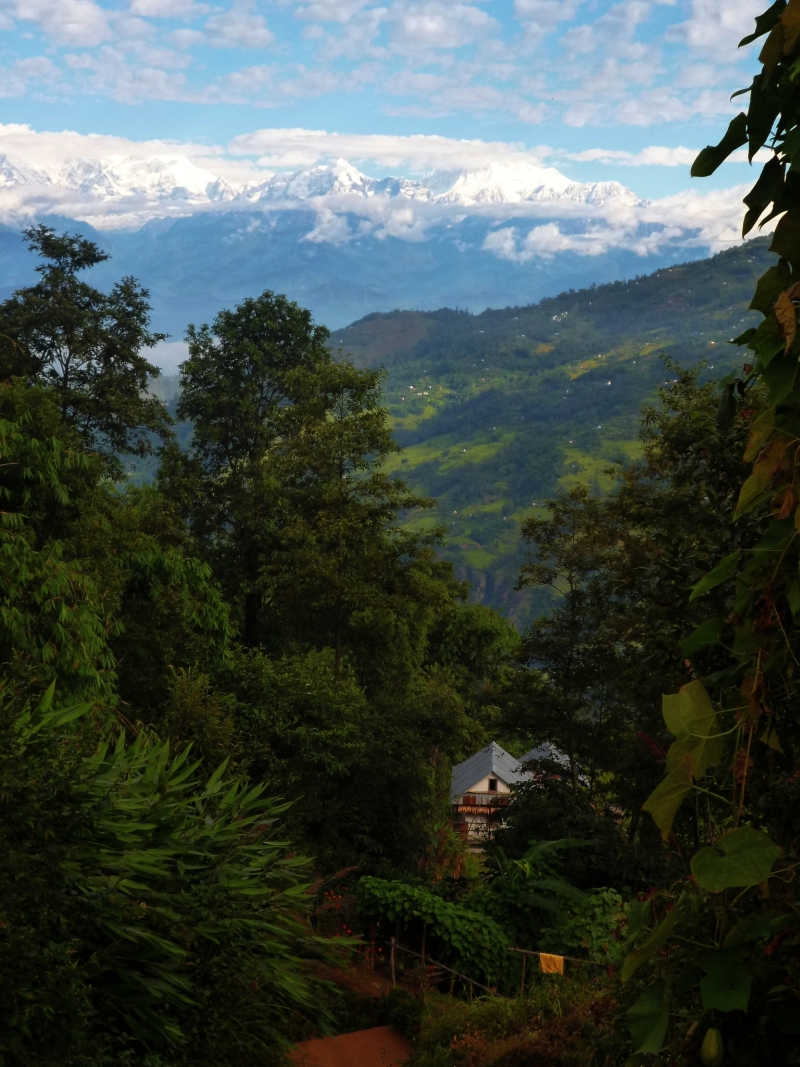
\includegraphics[width=6cm]{figures/tumok-path.jpg}
\caption{A typical trail in Tumok}\label{tumok-path}
\end{figure}

Geomorphic deixis permeates Yakkha grammar;  it features in a number of word classes and grammatical subsystems, in demonstratives, adverbs, postpositions,  verbs and even interjections.\footnote{Other Kiranti languages like Belhare, Bantawa or Khaling furthermore distinguish altitude in their locative case systems \citep{Ebert1994The-structure, Bickel1997Spatial}.} This shows how deeply rooted the geomorphic system is in the grammar of Yakkha, and how strongly environmental factors may shape a language.\footnote{The Yakkha system (and Kiranti languages in general) also shows that spatial orientation is by no means universally egocentric (based on the body of the speaker), as had been claimed before the discovery of geomorphic deixis.} \citet{Bickeletal1999Cultural} also point out the salience of the \rede{hill} conception in cultural domains such as architecture, rituals and mythology in the Kiranti cultural sphere. For Yakkha, this connection remains to be studied.

In the following, I will briefly lay out the system, before illustrating its application in each word class. Geomorphic forms in Yakkha are based on two sets of roots, called /u/-forms and /o/-forms in the following discussion. They indicate  a threefold distinction: words based on \emph{tu} and \emph{to} for \rede{uphill}, on \emph{mu} and \emph{mo} for \rede{downhill} and on \emph{yu} and \emph{yo} for \rede{across (at the same altitude)}. The distinction between the /u/-forms and the /o/-forms is one of deictic transposition, as in Belhare (see \citealt{Bickel1997Spatial, Bickel2001Deictic}). 

The schematic diagrams in \figref{deicticschema-1} and \figref{deicticschema-2} provide a bird's eye view on the deictic field, and the black dots indicate the speaker. In both sets, the deictic field is partitioned into four quadrants. In the /u/-forms, the point of reference  for projecting the four quadrants (indicated by \rede{⌀}) is located within the speech situation. Objects located uphill from the interlocutors are indicated by forms based on \emph{tu}, objects located downhill  from the interlocutors are indicated by forms based on  \emph{mu}, and objects on the same level (to either side of them) are indicated by forms based on \emph{yu} (see \figref{deicticschema-1}). Contrasts like left/right or front/back do exist in Yakkha, but they are rarely used in the expression of spatial orientation. The speakers are able to provide the lexemes when they are asked, but I have no instance of recorded natural speech using \emph{pheksaŋ} \rede{left} and \emph{chuptaŋ} \rede{right}. From the available lexical information, the left side is connoted negatively; it is used metaphorically in a term for a malicious wizard, for instance. This also  fits with the widespread perception of the left hand as impure in South Asian societies. The terms \emph{ondaŋ} \rede{front} and \emph{heksaŋ} \rede{back} are used more frequently than \rede{left} and \rede{right}. 


\begin{figure}
\centering
\setlength{\fboxsep}{0pt}
\fbox{
\begin{tikzpicture}[xscale=1, yscale=-1, draw=black, fill=black!30]
	\node (lo) at (-3,-3) {};
	\node (ro) at ( 3,-3) {};
	\node (lu) at (-3, 3) {};
	\node (ru) at ( 3, 3) {};
	\node (z)  at ( 0, 0) {\Large ⌀=●};
	\draw (lo)--(z);
	\draw (ro)--(z);
	\draw (lu)--(z);
	\draw (ru)--(z);
	\node (tu) at ( 0,-2) {tu};
	\node (yu1)at (-2, 0) {yu};
	\node (yu2)at ( 2, 0) {yu};
	\node (mu) at ( 0, 2) {mu};
\end{tikzpicture}
}
\caption{The deictic mapping system of the /u/-forms}\label{deicticschema-1}
\end{figure}

\bigskip

\begin{figure}
\centering
\setlength{\fboxsep}{0pt}
\fbox{
\begin{tikzpicture}[xscale=1, yscale=-1, draw=black, fill=black!30]
	\node (lo) at (-3,-3) {};
	\node (ro) at ( 3,-3) {};
	\node (lu) at (-3, 3) {};
	\node (ru) at ( 3, 3) {};
	\node (z)  at ( 0, 0) {\Large ⌀};
	\node (sp) at (-4, 0) {\Large ●};
	\path (sp.west)++(0,0) node[left]{\footnotesize(speaker)};
	\draw (lo)--(z);
	\draw (ro)--(z);
	\draw (lu)--(z);
	\draw (ru)--(z);
	\node (to) at ( 0,-2) {to};
	\node (khe)at (-2, 0) {khe};
	\node (yo) at ( 2, 0) {yo};
	\node (mo) at ( 0, 2) {mo};
\end{tikzpicture}
}
\caption{The transposed mapping system of  \emph{khe} and the /o/-forms}\label{deicticschema-2}
\end{figure}

\bigskip

\begin{figure}
\centering
\setlength{\fboxsep}{0pt}
\fbox{
\begin{tikzpicture}[xscale=1, yscale=-1, draw=black, fill=black!30]
	\node (l) at (-3, 0) {};
	\node (r) at ( 3, 0) {};
	\node (z)  at ( 0, 0) {\Large ⌀};
%	\node (sp) at ( 0, 4) {\Large ●};
% \path (sp.east)++(0,0) node[right]{\footnotesize(speaker)};
	\draw (l)--(z);
	\draw (r)--(z);
	\node (to) at ( 0,-2) {to};
	\node (mo) at ( 0, 2) {mo};
\end{tikzpicture}
}
\caption{Object-centered usage of \emph{mo} and \emph{to}}\label{deicticschema-3}
\end{figure}


In the /o/-forms, the point of reference for  projecting the four quadrants is transposed to a location that is not identical to the speech situation. The distinctions between \rede{uphill}, \rede{downhill} and \rede{across} are now determined from the perspective of this transposed point of reference (see \figref{deicticschema-2}; positioning  the speaker on the left side of the diagram was an arbitrary choice, he could as well have been posited on the right side; of course with a consequent reversal of \emph{yo} and \emph{khe}). Furthermore, if the transposed zero point is on the same elevation level as the interlocutors, a fourth root \emph{khe} comes into play, indicating the field between this new zero point and the speech situation. This field opens up only in the transposed system. The transposed zero point is important for generic statements and when the speaker talks about events he saw in movies, for instance. Given the transposed zero-point, it is only natural that there are more adverbs derived from the /o/-forms than from the /u/-forms. The  /o/-forms also serve as bases for spatial postpositions. Postpositions derived from the /u-/forms would only have the potential to locate objects with respect to the speech situation, not with respect to other objects.

The /o/-forms are also used to locate objects, or parts of objects, in relation to one another, for instance in order to determine the upper and the lower floor of a house, or in statements like \rede{I climbed up the tree}, where one abstracts away from the topography. In this object-centered system of spatial orientation, the location of the speech situation is irrelevant.  This is outlined in \figref{deicticschema-3}.  There are some fixed expressions like \emph{mokhaʔla-tokhaʔla} \rede{up and down} (lit.: \rede{down and up}). Similarly, \emph{yo} and \emph{khe} are used to convey contrasting directions on the same level (regardless of where the speaker is located), for instance in expressions like \emph{yokhaʔla-khekhaʔla} \rede{to and fro, back and forth}.

After this rather abstract characterization of the geomorphic orientation system of Yakkha, the remaining sections will illustrate how it is applied in each grammatical subsystem. Demonstratives (together with the interjections), are discussed in \sectref{dem-pron-2}, adverbs in  \sectref{geodeixis}, postpositions  in \sectref{geomorph-postp} and verbs in \sectref{geomorph-verb}.



\section{Demonstratives}\label{dem-pron-2}	

There are two sets of demonstratives, one featuring the the deictic /u/-forms and one featuring the transposed /o/-forms, as summarized in Tables \ref{mutuyu} and \ref{motoyo}. Structurally, these subsets are different from each other, too.  The /o/-forms are inherently adverbial and become nominal through nominalization with \emph{=na} ({\sc sg}) or \emph{=ha \ti =ya} ({\sc nsg/nc}). This is illustrated for \emph{to} in example \Next. These demonstratives can be used adnominally or pronominally. 
The /u/-forms are  essentially adverbs, too, but they can also be used as interjections, i.e. as proforms for clauses (see example \NNext). In this function they have a characteristic intonation. Uttered to attract the hearer's attention and to make him look in a particular direction, they are often accompanied by pointing gestures. The /u/-forms always locate an object with respect to the speech situation, i.e., the zero point is identical to the utterance context. This explains why the /u/-forms can combine with the proximal demonstratives, \emph{na} and \emph{kha} (cf. \sectref{dem-pron}),  to yield the topography-specific demonstratives shown in \tabref{mutuyu}. 

\begin{table}[htp]
\begin{centering}
\begin{tabular}{lll}
\lsptoprule
 {\sc direction} & {\sc root} & {\sc demonstrative}  \\
  & {\sc   ({\sc adv/interj})} & ({\sc sg/nsg, nc})\\
\midrule
{\sc up}&\emph{tu} &\emph{tunna/tukha}\\
{\sc across } &\emph{yu} &\emph{yunna/yukha}\\
{\sc down}&\emph{mu} &\emph{munna/mukha}\\
\lspbottomrule
\end{tabular}\\
\caption{Geomorphic demonstratives,  /u/-forms} \label{mutuyu}
\end{centering}
\end{table}


\begin{table}[htp]
\begin{centering}
\begin{tabular}{lll}
\lsptoprule
 {\sc direction} & {\sc root } & {\sc demonstrative} \\
  &(adv.) & ({\sc sg/nsg, nc})\\
\midrule
{\sc up}&\emph{to} &\emph{tona/toha} \\
{\sc across (beyond)}&\emph{yo} &\emph{yona/yoha} \\
{\sc across }&\emph{khe}&\emph{khena/kheha} \\
{\sc down}&\emph{mo} &\emph{mona/moha} \\
\lspbottomrule
\end{tabular}\\
\caption{Geomorphic demonstratives,  /o/-forms and  \emph{khe} }\label{motoyo}
\end{centering}
\end{table}


\ex. \ag. to khy-a!\\
uphill go{\sc -imp}\\
\rede{Go up!}
\bg. to=na paŋ\\
uphill{\sc =nmlz.sg} house\\
\rede{the upper house}


\ex.\ag.muǃ puchak!\\
{\sc int} snake\\
\rede{Look, down thereǃ A snakeǃ} 
\bg.tuǃ maŋmeǃ\\
{\sc int} eagle\\
\rede{Look, up thereǃ An eagleǃ} 


Examples of /u/-demonstratives are shown in \Next.  In \Next[a], the home of the person referred to by \emph{buddhini} is located on the same level as the speaker's home, where she is sitting at the time of speaking. Example \Next[b] is from a mythical story that takes place in the environment and the array of villages as they are today, and the place called Manglabare is uphill from the speech situation (in Tumok village). The /u/-forms are also used for microlocation, such as pointing out a spider to the downhill side of the speaker, even if it is located on the same elevation level (see \figref{deixill-1}).

\ex.\ag.nhaŋ    yunna              buddhini=ca        eko pi-ŋ\\
and\_then this\_across buddhist\_woman{\sc =add} one give{\sc [pst]-1sg.A}\\
\rede{And I gave one to the buddhist woman (living) over there.}\source{36\_cvs\_06.387}
\bg.ŋ-ikt-uks-u-ci=hoŋ   tunna    maŋlabare n-da-ya-by-a-ma	\\
{\sc 3pl.A-}chase{\sc -prf-3.P[pst]-3nsg.P=seq} this\_uphill Manglabare {\sc 3pl-}come{\sc -pst-V2.give-pst-prf}\\
\rede{As they (the Limbus) chased them (Lalubang and Phalubang), they  (the Limbus) already came up to Manglabare.} (lit. \rede{to Manglabare uphill}) \source{22\_nrr\_05.029}	



\begin{figure}
\centering
\setlength{\fboxsep}{0pt}
\fbox{
	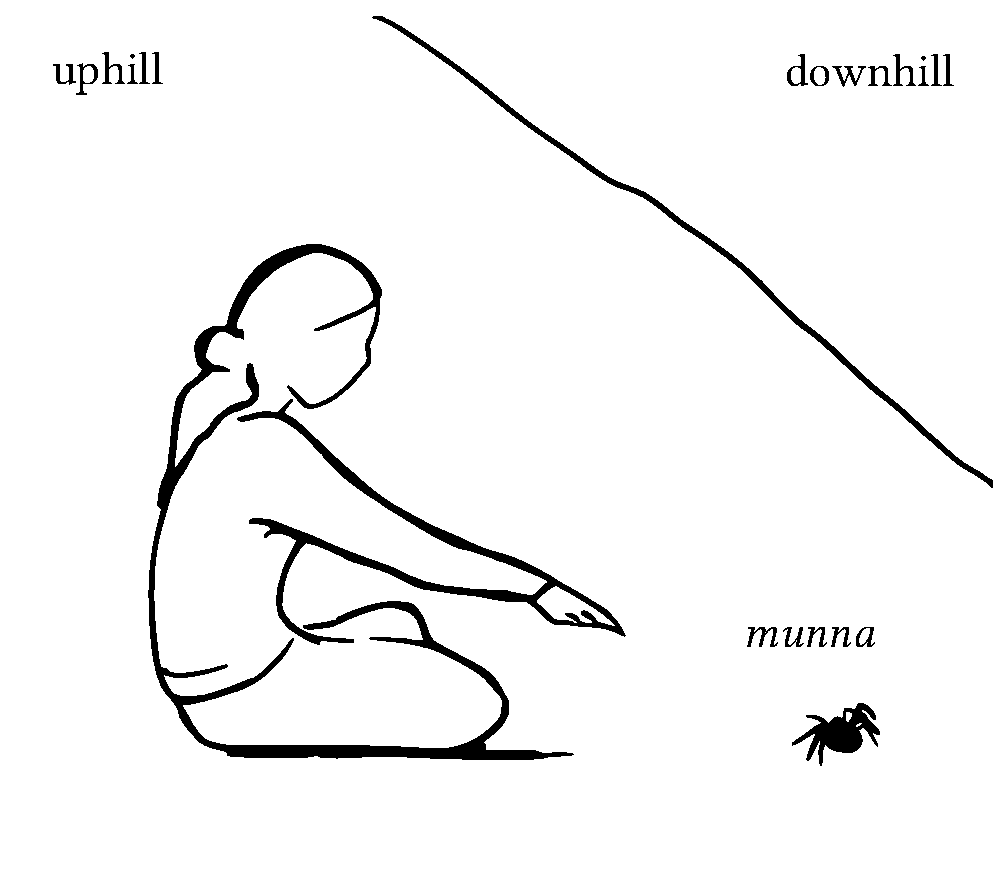
\includegraphics[width=7cm]{figures/deixill-1.eps}
}
\caption{The /u/-forms in practice}\label{deixill-1}
\end{figure}


	
	
In contrast, the /o/-forms are found in generic statements (see \Next[a]), and in procedural descriptions, that are detached from the here and now of the speech situation (see \Next[c]). They are also found in contexts that open up a secondary deictic field, such as in movies (see example  \Next[b] from a pear story). 

\ex.\ag.\label{mewamhabu}nhaŋ eko=bu,    mo=na tala=ca         me-wa-m=ha=bu\\
and\_then one{\sc =rep} downhill{\sc =nmlz.sg} floor{\sc =add} {\sc neg-}live{\sc -inf[deont]=nmlz.nsg=rep} \\
\rede{And one more thing: the Linkhas shall not live on the ground floor, too, it is said.} \source{11\_nrr\_01.040}
\bg. nhaŋŋa hon=na mamu=nuŋ, saikal=be ta-yatasa=na yo=na mamu=ca, nhaŋŋa khaʔla lukt-a-sy-a-ci,  men=na=i?	\\
	and\_then that\_very{\sc =nmlz.sg} girl{\sc =com} bicycle{\sc =loc} come{\sc [3sg]-pst.prog=nmlz.sg} across{\sc =nmlz.sg} girl{\sc =add} and\_then like\_this bump\_into{\sc -pst-mddl-pst-du} {\sc cop.neg=nmlz.sg=q}\\
\rede{And that earlier girl and the girl that was coming on the bike, they collided like this, right?}\footnote{The verb form \emph{tayatasa} could not be analyzed, as no corresponding paradigm could be elicited. According to the Nepali translations, I tentatively labelled it \rede{past progressive}.} \source{34\_pea\_04.025 }
\bg.to=na  paŋ=be     ku-nuŋ-ma, sin-di-me,  mo=na  paŋ=be     tha  n-leŋ-me-n, ka-ma pʌryo  ai?\\
up{\sc =nmlz.sg} house{\sc =loc} guard{\sc -V2.sit-inf[deont]} die{\sc -V2.give[3sg]-npst} downhill{\sc =nmlz.sg} house{\sc =loc} knowledge {\sc neg-}happen{\sc [3sg]-npst-neg}, say{\sc -inf[deont]} have\_to {\sc tag}\\
\rede{In the upper house, people keep sitting at the sickbed, someone dies eventually ‒ in the lower house, they have no idea, one has to tell them, right?}\footnote{This example refers to another Yakkha custom: firing rifles for announcements, in pairs to announce marriages, and in single shots to announce the death of a  member of the household. The choice of \emph{tona} and \emph{mona} in this example is arbitrary, it could as well be the other way round, as this is just an example made by the speaker to illustrate the custom; the sentence does not refer to any particular constellation of houses.} 	 \source{29\_cvs\_05.028}
   			
			
As pointed out in the introduction, the /o/-forms are also used when two objects are located with respect to each other, as in such cases the zero point is also not identical to the speech situation, but located between the related objects, such as in \Next. In this example, two people look downhill, seeing two swallows  sitting on a parallel wires (as illustrated in \figref{deixill-2}). Interlocutor A points out something about one of the  swallows and interlocutor B wants to reconfirm whether he got the reference right. The  zero point for the projection is located between the two birds. The demonstrative \emph{tona} refers to the bird closer to the hill on which the interlocutors are located and that serves as the anchor of the relation, and \emph{mona} refers to the bird on the wire  further away from that hill. If the swallows had been located uphill from the interlocutors, the question would have been exactly the same as the one uttered in \Next; the speech situation is irrelevant for the interpretation of this utterance.

\exg.\label{ex-gumthali}to=na=em mo=na=em?\\
uphill{\sc =nmlz.sg=alt} downhill{\sc =nmlz.sg=alt}\\
\rede{(Do you mean) the upper one or the lower one?}

\begin{figure}
\centering
\setlength{\fboxsep}{0pt}
\fbox{
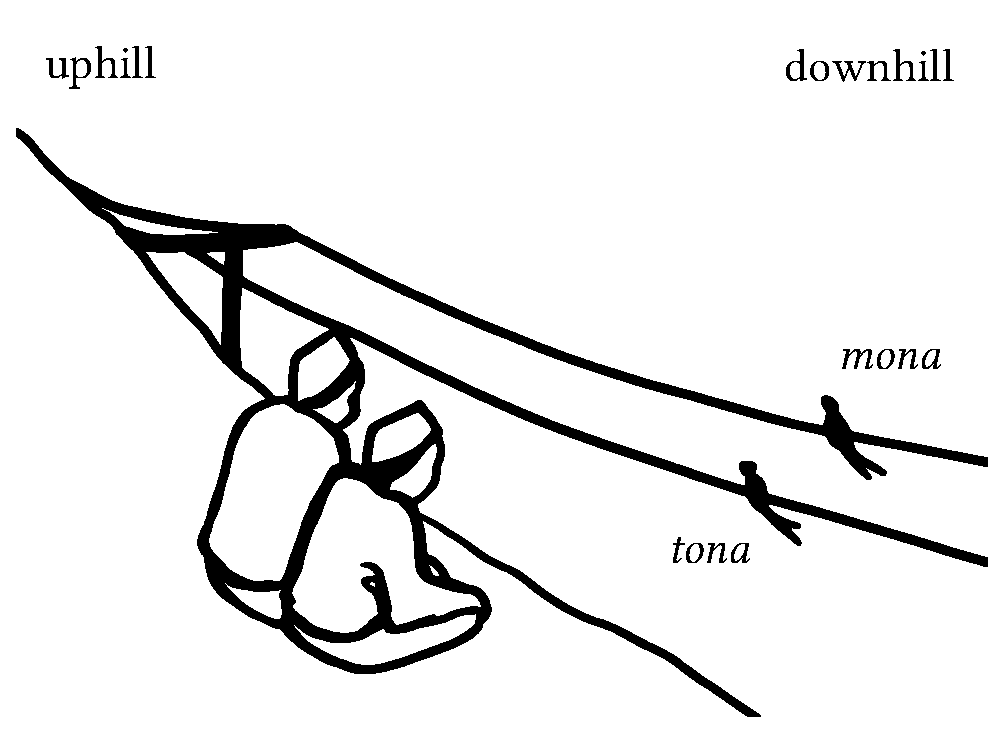
\includegraphics[width=7cm]{figures/deixill-2.eps}
}
\caption{Illustration for example \ref{ex-gumthali}}\label{deixill-2}
\end{figure}

The uphill-downhill distinction can also be mapped onto the human body, as in \Next. These designations are used regardless of the orientation of a person, thus instantiating an exception to the topography-based system.

\ex.\ag.mo=ha keŋ=ci \\
downhill{\sc =nmlz.nsg} tooth{\sc =nsg} \\
\rede{lower teeth}
\bg.to=ha keŋ=ci\\
uphill{\sc =nmlz.nsg} tooth{\sc =nsg} \\
\rede{upper teeth} 


Things look slightly different on the horizontal plane: in example \Next[a], two houses are identified  that are both on the same altitude level as the interlocutors. The house further away is referred to as \emph{yona}, the closer one is \emph{khena}, a distinction most closely rendered by \rede{there, thither} and \rede{here, hither} in the English translation (see also \figref{deixill-3}, which  features  \emph{mo} and \emph{to} as well). In \figref{deixill-3}, the couple in the foreground represents the speech situation.

\ex.\ag.\label{khenamenna}eh, khe=na paŋ menna, yo=na=le\\
oh across\_here{\sc =nmlz.sg} house {\sc neg.cop=nmlz.sg} across\_there{\sc =nmlz.sg=ctr}\\
\rede{Oh, not the closer house, the next oneǃ} 
 \bg. mela=be      yo   khe    son-ca-saŋ\\
market{\sc =loc} across\_there across\_here look{\sc -V2.eat-sim} \\
\rede{Looking around in the market, ...} \source{01\_leg\_07.152}
 
\begin{figure}
\centering
\setlength{\fboxsep}{0pt}
\fbox{
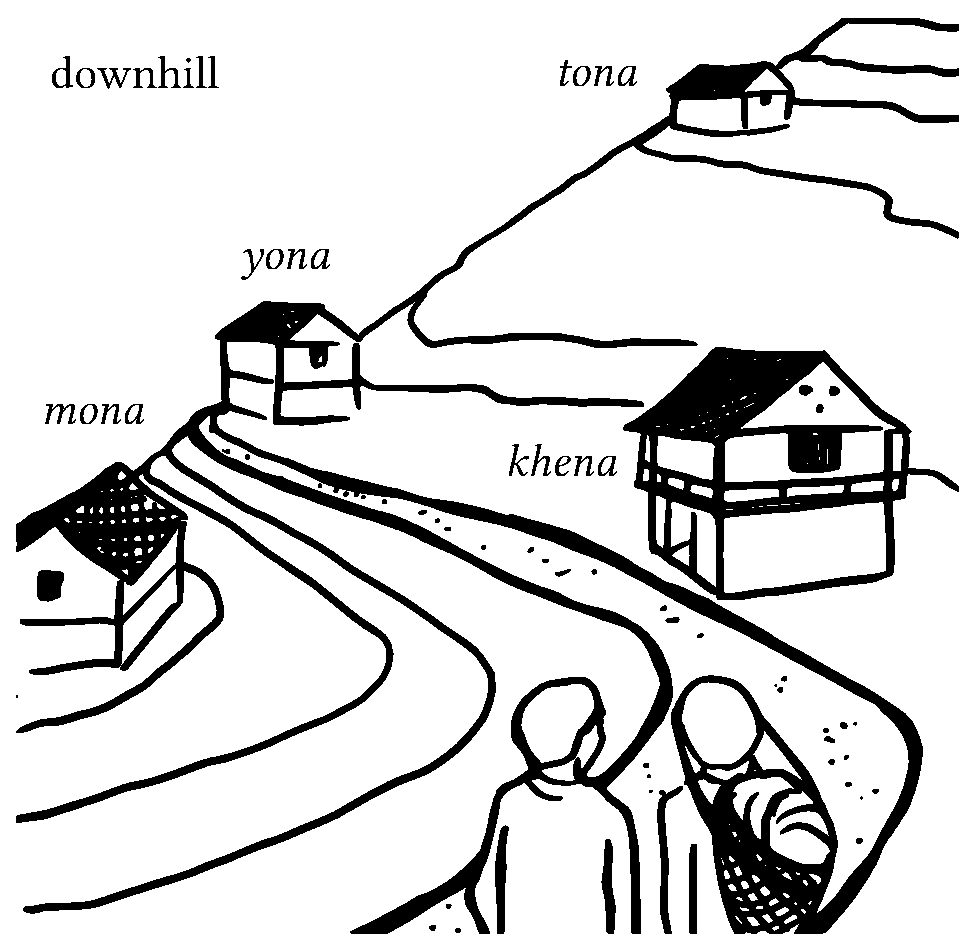
\includegraphics[width=7cm]{figures/deixill-3.eps}
}
\caption{The transposed system in practice}\label{deixill-3}
\end{figure}

The quadrant indicated by \emph{yo} is always beyond some (real or imagined) boundary on the horizontal level, i.e. it is projected from a zero point that must be distinct from the speech situation. The space between that boundary and the speech situation is the field indicated by \emph{khe}.\footnote{In this light, it also makes sense that \emph{khe} is never used in opposition to \emph{yu}. A \emph{khe}-quadrant opens up only when the zero point for the projection is transposed, while the field indicated by \emph{yu} projects directly from the speech situation.} In  example \Last[a], the  utterance context is relevant for the interpretation of \emph{yo} and \emph{khe},\footnote{Note that it is not the case that \emph{yona} always refers to the object between an upper and a lower object (the same is true for Belhare, see \citealt{Bickel2001Deictic}).  If the speakers were standing on the level of the lower house, the demonstrative referring to it would change from \emph{mona} to \emph{yona}.} while this is not the case for the \emph{mo/to} distinction in \LLast[b], for instance. As mentioned above, the \emph{yo}/\emph{khe}  contrast can also be used generically, independent  of any particular utterance context, as in example  \Last[b].
 
As the /u/-forms always rely on information that is retrievable from the utterance context, they are not compatible with the reportative marker \emph{=bu}. Thus, while \Next[a] is perfectly fine, \Next[b] is pragmatically awkward.\footnote{The reportative marker can also be found on embedded speech, both direct and indirect; see also \sectref{utterance-pred} and \sectref{hearsay}.} Another example for /o/-forms combining with \emph{=bu} is \ref{mewamhabu} above.

\ex.\ag. to=na minuma lukt-a-khy-a=na=bu?\\
uphill{\sc =nmlz.sg} cat run{\sc [3sg]-pst-V2.go-pst=nmlz.sg=rep} \\
\rede{It was said that the upper cat ran away?}
\bg.?tu-nna minuma lukt-a-khy-a=na=bu?\\
this\_uphill cat run{\sc [3sg]-pst-V2.go-pst=nmlz.sg=rep} \\
Intended: \rede{It was said that the cat up there ran away?}
 
The examples in \Next show that the proximal/distal demonstratives (see  \sectref{dem-pron-1}) and the \rede{uphill}/\rede{downhill} demonstratives are not mutually exclusive; they can be used together in one syntagm. The former indicate proximity or distance to the speaker, while the latter locate the objects with respect to each other and the cline of the hill. In \Next[a], the zero point is located between the upper and the lower rocks of a group of rocks, and in \Next[b], the zero point is located in the middle of the road.\footnote{As the proximal/distal demonstratives \emph{na/nna} show a functional overlap with \emph{khena} and \emph{yona}, these two sets are not expected to occur together.}

\ex.\ag.  na   mo=na  luŋkhwak\\
this downhill{\sc =nmlz.sg} stone\\
\rede{this lower rock (of a group of rocks)} \source{37\_nrr\_07.031}
\bg.mo=na  u-lap,          to=na  u-lap,          na   lambu ghak ak=ka=i!\\
downhill{\sc =nmlz.sg} {\sc 3sg.poss-}wing uphill{\sc =nmlz.sg}  {\sc 3sg.poss-}wing this road all {\sc 1sg.poss=gen=emph} \\
\rede{The uphill side, the downhill side, this road is all mine!}  \source{36\_cvs\_06.206}


The examples in \Next illustrate abstractions away from the closest hill as the achoring element. In \Next[a],  \emph{mu} refers to a place outside the hills and far away (Germany). In \Next[b], via reduplication of the initial CV-cluster, the root  intensifies its meaning, i.e. \emph{tutunna} refers to an object further away than \emph{tunna}. These reduplications are also found in the corresponding adverbs (see \sectref{geodeixis} below). 

\ex. \ag. mu, [...] nniŋ=ghe i=ha cog-wa-m-g=ha?\\
	downhill [...] {\sc 2pl.poss=loc} what{\sc =nmlz.nsg} do{\sc -npst-2pl.A-2=nmlz.nsg}\\
	\rede{Downhill, where you live, what do you do (when someone dies)?} \source{29\_cvs\_05.008}
\bg. tunna cokcoki=nuŋ tu-tunna cokcoki\\
		that\_uphill star{\sc =com}	{\sc redup-}that\_uphill star\\
	\rede{the star up there and the star even further up}


\section{Adverbs}\label{geodeixis}

This section discusses the adverbs that belong to the geomorphic  orientation system. In \sectref{dem-pron} a set of adverbs has been introduced that is based on a proximal/distal/anaphoric distinction. The adverbs discussed in the following are based on the same distinctions between /o/-forms and /u/-forms as the demonstratives discussed in \sectref{dem-pron-2} above. 
Tables \ref{deic-all1} and \ref{deic-all2}  provide an overview of all geomorphic adverbial expressions in Yakkha. 
	 	  
 \begin{table}[htp]
\begin{centering}
\begin{tabular}{llll}
\lsptoprule
									&{\sc up}		&{\sc across}&{\sc down}\\
\midrule
			{\sc loc/interj}	&\emph{tu}&\emph{yu}&\emph{mu}\\
			{\sc loc-prox}&\emph{tunhe}&\emph{yunhe}&\emph{munhe}\\
			{\sc loc-dist}&\emph{tunnhe}&\emph{yunnhe}&\emph{munnhe}\\
			{\sc loc-dist-emph}&\emph{tutunnhe}&\emph{yuyunnhe}&\emph{mumunnhe}\\
\lspbottomrule
\end{tabular} 
\caption{Geomorphic adverbs, the /u/-forms}\label{deic-all1}
\end{centering}
\end{table}

 \begin{table}[htp]
\begin{centering}
\begin{tabular}{lllll}
\lsptoprule
									&{\sc up}		&\multicolumn{2}{l}{{\sc across}}&{\sc down}\\
											&				&{\sc prox}&{\sc dist}&\\
\midrule 	  
			{\sc loc/dir}	&\emph{to}&\emph{khe}&\emph{yo}&\emph{mo}\\
			{\sc dir} 				&\emph{tokhaʔla}&\emph{khekhaʔla}&\emph{yokhaʔla}&\emph{mokhaʔla}\\
			{\sc abl/dir}											&\emph{tondaŋ}&\emph{khendaŋ}&\emph{yondaŋ}&\emph{mondaŋ}\\
			{\sc level}											&\emph{topparik}&\emph{khepparik}&\emph{yopparik}&\emph{mopparik}\\
			{\sc level-abl}									&\emph{topparindaŋ}&\emph{khepparindaŋ}&\emph{yopparindaŋ}&\emph{mopparindaŋ}\\
			{\sc quant} 					&\emph{torok}&\emph{kherek}&\emph{yorok}&\emph{morok}\\
			{\sc quant-emph}								&\emph{toʔtorok}&\emph{kheʔkherek}&\emph{yoʔyorok}&\emph{moʔmorok}\\
			{\sc loc-prox}									&\emph{naʔto}&\emph{naʔkhe}&\emph{naʔyo}&\emph{naʔmo}\\
			{\sc loc-dist}										&\emph{nnaʔto}&\emph{nnaʔkhe}&\emph{nnaʔyo}&\emph{nnaʔmo}\\
			{\sc loc-prox-quant}					&\emph{naʔtorok}&\emph{naʔkherek}&\emph{naʔyorok}&\emph{naʔmorok}\\
\lspbottomrule
\end{tabular} 
\caption{Geomorphic adverbs, /o/-forms and \emph{khe}}\label{deic-all2}
\end{centering}
\end{table}


The adverbs based on the proximal/distal distinction are \emph{nhe} \rede{here} (see \Next[a]) and \emph{nnhe} \rede{there} (with initial gemination of the nasal). The adverb \emph{nnhe} is used to refer to distant locations and to locations in another deictic field, as it is opened up by a movie, for instance  (see \Next[b] from a pear story) or by talking on the phone. The anaphoric form is \emph{honnhe} \rede{just there, at a location mentioned earlier} (see also \sectref{dem-set1rel}). 

\ex. \ag. imin=na,       haku nhe, hen=se;         haku soʔ-ma=na=lai!\\
how{\sc =nmlz.sg}  now here today{\sc =restr} now look{\sc -inf[deont]=nmlz.sg=excla}\\
\rede{How is he; now he (the prospective groom) is here, only today; now we have to look at him!}  \source{36\_cvs\_06.374}
\bg.ɖhakani=be    s-wa,         nnhe  eko man=na \\
basket{\sc =loc} look{\sc -npst[3sg.P]} there one {\sc cop.neg=nmlz.sg}\\
\rede{He looks into the basket, and there is not even one.} \source{34\_pea\_04.040 }


These proximal and distal adverbs can be specified further by combining them with the /u/-forms of the geomorphic set, in the same way as it has been shown above for the demonstratives. Both sets rely on the utterance context, and are, therefore, compatible. Altogether, one arrives at three more forms for each  \rede{here} and \rede{there}: \emph{tunhe/tunnhe} \rede{up here/there}, \emph{munhe/munnhe} \rede{down here/there} and \emph{yunhe/yunnhe} \rede{across here/there}. The resulting complex forms are illustrated by the examples in \Next. 

\ex.\ag.\label{tikamunhe}ŋkha=nuŋ   nhe  gobar,   pik=ka    u-hi,    bachi=ga,        goru=ga    men=na,    munhe     khaʔla   yuŋ-ma=hoŋ      ʈika    waʔ-meʔ-ma  \\
that{\sc =com} here cow\_dung cow{\sc =gen} {\sc 3sg.poss-}shit cow{\sc =gen} ox{\sc =gen} {\sc neg.cop=nmlz.sg} down\_here like\_this put{\sc -inf=seq} blessing wear{\sc -caus-inf[deont]}\\
\rede{With this (\emph{dubo} grass), here, cow dung, from a female cow, not from an ox, one has to place it down here like this and apply a blessing (at the main door of the house).} \source{31\_mat\_01.089}
\bg.munnhe     sombare  daju=ge            ŋ-waʔ=ya=ci=bu,                      hau   jeppa!\\
down\_there Sombare eB{\sc =loc} {\sc 3pl-}exist{\sc =nmlz.nsg=nsg=rep} {\sc excla} really\\
\rede{Oh! Sombare brother down below has some (mushrooms), they say, really!} \source{13\_cvs\_02.079}
\bg. ka=go      tunnhe   bhitta=be    heʔ-ma-sy-a-ŋ=na=le,   a-na=ŋa,     uks-a-ga=i,       uks-a ly-a-ŋ=hoŋ\\
{\sc 1sg=top} up\_there wall{\sc =loc} cut{\sc -inf-aux.prog-pst-1sg=nmlz.sg=ctr} {\sc 1sg.poss-}eZ{\sc =erg} come\_down{\sc -imp-2=emph} come\_down{\sc -imp} tell{\sc -pst-1sg=seq}\\
\rede{I was cutting (grass) up there at the wall, but my elder sister said: please come down, come down, ...} \source{28\_cvs\_04.315}

As example \Next shows, the /u/-forms can also be used independently, in adverbial function. 

\exg.mu     jeʈha=ŋa   biha     cog-a             bhoŋ, mu     jeʈha=ŋa            hiŋ-ma=na\\
down first\_born\_male{\sc =erg} marriage do{\sc [3sg]-sbjv} {\sc cond} down first\_born\_male{\sc =erg} support{\sc -inf[deont]=nmlz.sg}\\
\rede{If Jetha down here marries a girl, he has to care for her.} (pointing to someone sitting in the same room as the speaker, but in the corner pointing downhill) \source{28\_cvs\_04.127}


A natural example of a reduplicated form is shown in \Next. Typically, the reduplicated forms contrast an object further away with a closer object. In this example, however, the emphasis usually connected to this reduplication is not very strong;  in the afterthought at  the end of the sentence, the simple form \emph{tunnhe} is used.\footnote{The mirative (see \sectref{ptcl-evid})  is used here because the speaker finally remembers where she had been at a particular day some weeks prior to this conversation.} For instance, if the speaker points downhill towards two houses, the closer location is indicated by \emph{munnhe} \rede{down there} and the one further down is indicated by \emph{mumunnhe} \rede{further down there}. 

	\exg. ka  ŋkhaʔla bhoŋ tu-tunnhe         bhauju=ghe               wa-ya-masa-ŋ=na                        raecha, tunnhe=ba\\
	{\sc 1sg} like\_that {\sc cond} {\sc redup}-there\_uphill sister-in-law{\sc =loc} be{\sc -pst-pst.prf-1sg=nmlz.sg} {\sc mir} there\_uphill{\sc =emph}\\
\rede{If it is like that, I had been uphill at my sister-in-law's house, just up there.} \source{36\_cvs\_06.399}


The /o/-forms are used when the zero point is not located within the speech situation. Thus, they cannot combine in one word with the deictic forms \emph{nhe} and \emph{nnhe}. They can combine with other morphology, e.g. with case markers, to convey a variety of spatial notions, such as ablative and directive, shown in \Next. The roots \emph{mo}, \emph{to} and \emph{yo} are inherently locative, so that they cannot combine with the locative \emph{=pe} (for instance, *\emph{mobe} is ungrammatical). Forms as in \Next[a] can be used both with an ablative and a directive reading.

\ex. \ag.mondaŋ ky-a=na.\\
from\_below come\_up{\sc [3sg]-pst=nmlz.sg}\\
\rede{He came up from below.}
\bg. yondaŋ    eko mamu a-cya            we=ppa=ʔlo!\\
from\_over\_there one girl {\sc 1sg-}child exist{\sc [3sg;npst]=emph=excla}\\
\rede{(But) I have a daughter from (my ex-husband) over there!} \source{06\_cvs\_01.018}
\bg.tokhaʔla khy-aǃ\\
upwards go{\sc -imp}\\
\rede{Go upwardsǃ}

The contrast between \emph{yo} and \emph{khe} (see also \figref{deicticschema-2} above) can be illustrated by the following context: the two villages Madi Rambeni and Madi Mulkharka are both located on a hill next to the hill on which Tumok is situated (see also the Map in \figref{map-sank} in \sectref{geogr}). These two hills are separated by a river (the Maya Khola), and thus both Madi Rambeni and Madi Mulkharka qualify as \emph{yo} \rede{across} from Tumok. Both villages are roughly on the same altitude level as Tumok, but while Madi Mulkharka is right across (one can see its houses), Madi Rambeni is further away and out of sight. Thus, in a conversation (in Tumok) contrasting the two villages, Madi Mulkharka would be indicated by \emph{khe}, while Madi Rambeni would be referred to by \emph{yo}, since it is further away from Tumok  than Madi Mulkharka.

Another set of adverbs is instantiated by adverbs such as \emph{mopparik} \rede{right below} in \Next. It refers to a place that is right below the point of reference, like a lower floor or a lower step on a ladder (\emph{-parik} comes from the Nepali noun \emph{paṭī} \rede{side}).\footnote{The change of  coronal plosives to rhotics in intervocalic position is also attested elsewhere in the language, and closing a word-final CV syllable with /k/ is a common process in the \rede{Yakkhafication} of lexical material from Nepali, see \sectref{loansphon}.} This set of adverbs, like the forms in \Last, can also be used  as  postpositions (see \sectref{geomorph-postp} below). 

\exg. honna              sem-khuba        babu, pheri, i=ʔlo       mopparik    jhar-a          cok-ma-sy-a=na\\
that\_very pluck{\sc -nmlz} boy again what{\sc =excla} right\_below descend{\sc -nativ} do{\sc -inf-aux.prog-pst[3sg]=nmlz.sg} \\
\rede{That guy who was plucking, he was climbing down (the ladder).} \source{34\_pea\_04.036}


Furthermore, there are forms ending in the syllable \emph{-rok \ti -rek}, i.e. \emph{morok}, \emph{torok}, \emph{yorok} and \emph{kherek}. They convey that something is located (or moving) a bit more in the respective direction than had been presupposed, thus quantifying the distance (see \Next). Example \NNext illustrates the same with ablative forms. 

\ex. \ag.hoŋkhaʔniŋŋa   naʔmasek    khi-khuwa          yapmi=ci     yorok      torok      ŋ-wa-ya-masa\\
that\_very\_time night fight{\sc -nmlz} person{\sc =nsg} a\_bit\_further a\_bit\_up {\sc 3pl-}be{\sc -pst-pst.prf}\\
\rede{At that time, those fighting people had been (scattered) a bit further away and a bit further uphill.} \source{41\_leg\_09.057}
\bg.nna  ten=be=jhen,         mo,   yondaŋ    morok=ŋa       limbu=ci=ca           ŋ-wa-ya-ma\\
that village{\sc =loc=top} down from\_across a\_bit\_down{\sc =ins} Limbu\_person{\sc =nsg=add} {\sc 3pl-}be{\sc -pst-prf}\\
\rede{In that village below, across and then a bit below from there, Limbu people were  living, too.} \source{22\_nrr\_05.009}

\ex. \ag.mondaŋ kham ket-u-eba\\
from\_below ground bring\_up{\sc -3.P[imp]-pol.imp}\\
\rede{Bring up mud from below.}
\bg.miyaŋ morondaŋ ket-u-eba\\
a\_little from\_further\_below bring\_up{\sc -3.P[imp]-pol.imp}\\
\rede{Bring it up from a bit further below.} (Context: the mud is better further downhill.)

The adverbs ending in \emph{-rok\ti -rek} can also be partly reduplicated, yielding forms like \emph{moʔmorok} or \emph{toʔtorok}. Tentatively, in analogy to the reduplications discussed above, I conclude that this amplifies the distance, too, but there are not enough examples in my data for any strong claims. The reduplicated forms are also  used when nothing has been presupposed (cf. also \sectref{geomorph-postp} on postpositions).
 
\exg.  beuli siŋgara         cok-se         miyaŋ yoʔyorok ŋ-ghet-wa\\
bride a\_wedding\_custom do{\sc -sup} a\_little a\_bit\_further {\sc 3pl.A-}take{\sc -npst[3.P]}\\
\rede{To dress the bride with the sari that the groom got her, they take her a bit further away.} \source{25\_tra\_01.043}


The last set of adverbs introduced here has  the forms \emph{naʔmo}, \emph{nnaʔmo}, \emph{naʔyo}, and so on. They are composed of the singular forms of the proximal/distal demonstratives and the /o/-forms, conveying \rede{down here}, \rede{down there}, \rede{across here} and so on (see \tabref{deic-all2}).  The cognate forms in Belhare are demonstratives that are marked for environmental case (see \citealt[226--27]{Bickel2001Deictic}). The environmental case system was probably present in earlier stages of Yakkha, too, but apart from these adverbial forms, there is no trace of such a system synchronically. The forms have characteristic stress, i.e. on the first syllable. They locate the utterance context from the perspective of another location. In \Next[a], the zero point is Manglabare, a place above Tumok (the place of speaking, referred to by \emph{naʔmo} \rede{down here}). In \Next[b], the point of reference is the sky, mentioned in the adverbial clause.  The sentence in \Next[c] was uttered by someone who confused two roads, and the point of reference is the point of departure of the speaker's movement, before she confused the roads.

\ex. \ag.haku nnakha lalubaŋ=nuŋ   phalubaŋ=ga    ten=go         naʔmo=maŋ      sa,     eŋ=ga=e\\
now those Lalubang{\sc =com} Phalubang{\sc =gen} village{\sc =top} down\_here{\sc =emph} {\sc cop.pst[3sg]} {\sc 1pl.incl.poss=gen=loc}\\
\rede{Now, that village of Lalubang and Phalubang, though, was down  here, in our area.} \source{22\_nrr\_05.034}
\bg. na   taŋkheŋ=be    pes-a-khy-a-ma=niŋa naʔmo heko=ha nwak=ci=ŋa haku nda nhe uŋ-ma n-dokt-wa-ga-n=na n-lu-ks-u\\
	this sky{\sc =loc} fly{\sc -pst-V2.go-pst-prf[3sg]=ctmp} down\_here other{\sc =nmlz.nsg} bird{\sc =nsg=erg}	now {\sc 2sg} here come\_down{\sc -inf} {\sc neg-}get\_to\_do{\sc -npst-2.A[3.P]-neg=nmlz.sg} 	{\sc 3pl.A}-tell-{\sc prf-3.P[pst]}\\
	\rede{When he flew up into the sky, down here the other birds told him: Now you will not get the chance to come down here any more.} \source{21\_nrr\_04.034--5}
\bg.	naʔyo=le             sa-ŋ=na,                 nnaʔyo=le             khy-a-ŋ=na?\\
over\_here{\sc =ctr} {\sc cop.pst-1sg=nmlz.sg} over\_there{\sc =ctr} go{\sc -pst-1sg=nmlz.sg}\\
\rede{But I was over here, did I go over there?} \source{28\_nrr\_04.030}

\todo{Please check whether -- is used correctly in \textbackslash source. I suppose 034--5 is a range, but it could be s.th. different. Please do confirm it is a range.}

With the introduction of these forms, one arrives at two sets that are translatable as \rede{down/up/across here} and \rede{down/up/across there}, for instance \emph{naʔmo}  and forms like  \emph{munhe} for \rede{down here}. The  contrast between forms like  \emph{naʔmo}  and  \emph{munhe} is, of course, the zero point. While \emph{naʔmo} implies a perspective from a location outside the speech situation (see \Last and \Next), \emph{munhe} refers to a location in the downhill quadrant, as projected from the perspective of the speaker (see e.g. examples \ref{tikamunhe}—(c) above).  The speaker can choose whether he wants to locate objects from his own perspective or from someone else's perspective, and sometimes this is fixed by sociolinguistic conventions. In imperatives, for instance, it would be inappropriate to use one's own perspective, they are always expressed with /o/-forms, as in \Next. 

\ex. \ag.naʔyo ab-a\\
over\_here come\_across{\sc -imp}\\
\rede{Come over here (from where you are).}
\bg.naʔmo uks-a\\
down\_here come\_down{\sc -imp}\\
\rede{Come down here (from where you are).}


The \rede{quantifying} or \rede{degree} derivation via \emph{-rok} that was introduced above is also possible with \emph{naʔto} (and the related forms), yielding forms like \emph{naʔtorok} \rede{a bit closer up here}.



\section{Postpositions}\label{geomorph-postp}

The geomorphic postpositions are formally identical to the adverbs described in \sectref{geodeixis}. They take nominal complements that are marked by the genitive case (see \sectref{case-gen}). The possessive prefix is, however, not possible on these postpositions, which distinguishes  them from relational nouns (cf. \sectref{postpos-2}). \tabref{relnoun-topo} provides an overview on the postpositions.

 \begin{table}[htp]
\begin{centering}
\begin{tabular}{lll}
\lsptoprule
{\sc postposition}&{\sc gloss}&{\sc internal structure}\\
\midrule
\emph{mopparik} &right below&\rede{downhill-side[Nep.]}\\
\emph{topparik} &right above&\rede{uphill-side[Nep.]}\\
\emph{yopparik} &right across&\rede{across-side[Nep.]}\\
\emph{mokhaʔla} &below, downwards&\rede{uphill-{\sc dir}}\\
\emph{tokhaʔla} &above, upwards&\rede{uphill-{\sc dir}}\\
\emph{yokhaʔla} &across, away&\rede{across-{\sc dir}}\\
\emph{mondaŋ} &from below&\rede{downhill-{\sc abl}}\\
\emph{tondaŋ} &from above&\rede{uphill-{\sc abl}}\\
\emph{yondaŋ} &from the same level&\rede{across-{\sc abl}}\\
\emph{moʔmorok} &a bit below&\\
\emph{toʔtorok} &a bit above&\\
\emph{yoʔyorok} &a bit further away&\\
\emph{kheʔkherek} &a bit closer&\\
\lspbottomrule
\end{tabular} 
\caption{Geomorphic postpositions}\label{relnoun-topo}
\end{centering}
\end{table}

The postpositions \emph{mopparik} and \emph{topparik} indicate a relation of parallel planes located above/below each other, such as stacked books or floors of a house (see \Next[a]). Example \Next[b] shows a corresponding adverbial in a (semi-transparent) ablative form.\footnote{In analogy to these examples, one could assume that  there is also a directional \emph{topparikhaʔla}/\emph{mopparikhaʔla} to indicate directedness towards an upper/lower level, but such forms do not exist. Probably, \emph{topparik} (and related forms) also have a directional meaning.}  The same is possible with \emph{yopparik} and \emph{khepparik} on the horizontal level.

If the speaker wants to express that an object  is oriented towards a particular direction, the directional forms \emph{tokhaʔla}, \emph{mokhaʔla}, \emph{yokhaʔla} and \emph{khekhaʔla}  are used; orientation away from another object is indicatd by the ablative forms  \emph{tondaŋ}, \emph{mondaŋ},   \emph{yondaŋ} and \emph{khendaŋ}  (see \NNext).
 
\ex. \ag.ʈebul=ga mopparik\\
table{\sc =gen} right\_below\\
\rede{below the table (on a lower level, e.g. on the ground)}
\bg.kanciŋ mopparindaŋ ky-a-ci=ha\\
{\sc 1du} from\_right\_below come\_up{\sc -pst-du=nmlz.nsg}\\
\rede{We came up from the lower floor.}

\ex. \ag.ʈebul=ga tokhaʔla\\
table{\sc =gen} upwards\\
\rede{above the table (e.g. a lamp installed on the wall)}
\bg. ʈebul=ga mondaŋ chwigam kept-u=na\\
table{\sc =gen} from\_below chewing\_gum  glue{\sc -3.P[pst]=nmlz.sg}\\
\rede{Someone stuck chewing gum below the table.}

The partly reduplicated forms \emph{moʔmorok, toʔtorok} and \emph{yoʔyorok} convey that an object is located a bit in the respective direction, from the perspective of the object referred to by the complement noun (see \Next).

\ex. \ag.uŋci-paŋ=ga           moʔmorok          eko hoŋma wei-sa=na\\
{\sc 3nsg.poss-}house{\sc =gen}  bit\_downhill one river exist{\sc -pst[3sg]=nmlz.sg}\\
\rede{A bit downhill from their house there was a river.} \source{01\_leg\_07.283}
\bg.hon=na         yuktham=ga    yoʔyorok     kheʔkherek\\
that\_very{\sc =nmlz.sg} place{\sc =gen} bit\_further bit\_closer\\
\rede{around that place/the surroundings of that place} \source{01\_leg\_07.269}
		
		

\section{Motion verbs}\label{geomorph-verb}

Several motion verbs have also lexicalized the uphill/downhill distinction, as shown in example \Next and in \tabref{deic-verb}. Event specification with regard to the topography is highly frequent. Even though neutral forms are available (also included in the table), the pragmatically expected forms are those specifying the event for the \emph{mo/to/yo} distinction. This specificity reaches well beyond \rede{classical} motion events. Small-scale motions, too, like putting, repairing, stacking, looking, turning or calling are often precisely specified with respect to their spatial orientation. This is achieved by means of complex predicates  with different function verbs  (see \Next[b] and \tabref{V2-table} in Chapter \ref{verb-verb}). Motion away from a point of reference is not specified with respect to the topography, there are only the neutral verbs \rede{go} and \rede{carry off}. This is unexpected pragmatically: in motion events towards a point of reference, the speaker and the hearer are usually identifiable, and with them, the direction of the movement. In motion events away from a point of reference, as in \rede{go} and \rede{carry off}, the direction of the movement is less predictable, and therefore, it would be  more important pragmatically to specify events of going with regard to the topography-based distinctions.
 

\begin{table}[htp]
\begin{centering}
\begin{tabular}{lll}
\lsptoprule
 & {\sc come} &  {\sc bring}  \\
\midrule
{\sc neutral}&\emph{ta} \rede{come} (from a greater distance)& \emph{taʔ} \rede{bring}\\
{\sc neutral}&\emph{kheʔ} \rede{go} & \emph{khet} \rede{carry off}\\
{\sc up}&\emph{keʔ} \rede{come up}& \emph{ket} \rede{bring up}\\
{\sc across}&\emph{ap} \rede{come} (same level, small distance)& \emph{apt} \rede{bring}\\
{\sc down}&\emph{uks \ti uŋ} \rede{come down}&\emph{ukt} \rede{bring down} \\
\lspbottomrule
\end{tabular}
\caption{Geomorphic distinctions in motion verbs}\label{deic-verb}
\end{centering}
\end{table}


\ex. \ag.kanciŋ  to  tub-i=hoŋ          uks-a-ŋ-ci-ŋ=hoŋ                       yo      tas-a-ŋ-c-u-ŋ=ba\\
{\sc 1pl} up meet{\sc -1pl=seq} come\_down{\sc -pst-excl-du-excl=seq} across arrive{\sc -pst-excl-du-3.P-excl=emph}\\
\rede{Having met  uphill (many people), we (two) came down (home) and arrived across (at a neighbour's house on the same level as the speaker's home).} \source{36\_cvs\_06.395}
\bg.na   eko=ŋa=go       thend-u-get-uks-a=ba,     nna, om     leks-a=niŋa\\
this one{\sc =erg=top} lift{\sc -3.P-V2.bring\_up-3.P-prf-pst=emph} that bright become{\sc -pst[3sg]=ctmp}\\
\rede{One of them lifted it (the rock) and carried it up (holding in his hands, not carrying on his back), while the sun came out.} \source{37\_nrr\_07.086}


These topography-specific verbs are only compatible with suitable adverbial expressions. For instance, \emph{apma} \rede{come over} can only be used with \emph{yondaŋ}  \rede{from a location on the same altitude level}. Interestingly, this verb is also used when \rede{coming over} implies climbing down 800 meters, crossing a river and then climbing up on the other side again.


%  \chapter{Verbal inflection}\label{verbalmorph}

This chapter deals with the inflectional morphology of the Yakkha verb. Word formation on the verb level is treated in  Chapter \ref{verb-verb} on complex predicates, and in §\ref{trans-op} on transitivity operations.

The verbs can be grouped according to their stem forms and alternations (treated in §\ref{stem}). Most verbal roots have a pre-vocalic and one or more pre-consonantal  forms. There are lexical alternations and those that can be explained with morphophonological processes such as elision, voicing and assimilation. 

Yakkha verbal inflection is highly polysynthetic and overwhelmingly suffixing; the verb can carry up to seven suffixes, while there is only one prefix slot. The finite verb is  inflected for person and number of subject and object (treated in §\ref{verb-infl}), polarity (§\ref{neg}),  tense/aspect (§\ref{tense}) and  mood (§\ref{mood}). Politeness or honorific distinctions are not grammaticalized in the Tumok dialect, except for the imperative, which has an additional politeness register. In the Dandagaun dialect,  there is an honorific construction which is calqued upon the Nepali honorific verbal inflection  (§\ref{honorific}). The inflection of the copular verbs slightly deviates from the regular verbal inflection; it is treated in §\ref{cop-infl}. Two further verbal markers that do not fit elsewhere (the nativizer \emph{-a} and the knowledge marker \emph{-les})  are treated in §\ref{furtherverbal}. The finite verb stands in opposition to infinitives, converbs and nominalizations that are restricted to polarity and, occasionally, number inflection (see §\ref{nonfiniteforms}). 



Table \ref{abc} shows an overview of the most important verbal affixes in the regular verbal paradigm, and Table \ref{xyz} shows schematically how all  markers are distributed over the inflectional slots. Except for some idiosyncrasies in the inflection of copulas, there are no inflectional classes; all differences in inflectional behavior can be explained by morphophonology. 


\begin{table}[p]
\begin{centering}
\begin{tabular}{ll}
\lsptoprule
\multicolumn{2}{c}{ {\scshape person-number}}\\
\midrule
\emph{-ŋ}&1\\
\emph{-ka}&2\\
\emph{-u}&3.P\\
\emph{-nen}&1>2\\
\emph{-i}&1/2 plural\\
\emph{-ci}&dual  or 3 nonsingular P \\
\emph{N-}&3 plural S/A\\
\emph{=na}&singular\\
\emph{=ha}&nonsingular or non-countable\\
\midrule
\multicolumn{2}{c}{ {\scshape tense-aspect}}\\
\midrule
\emph{-meʔ/-wa}&nonpast\\
\emph{-a}&past\\
\emph{-ma/-uks}&perfect\\
\emph{-masa/-uksa}&past perfect\\
\emph{-siʔ}&progressive\\
\midrule
\multicolumn{2}{c}{ {\scshape negation}}\\
\midrule
\emph{N-...-n}&\\
\emph{-nin}&plural negation\\
\midrule
\multicolumn{2}{c}{ {\scshape mood}}\\
\midrule
\emph{-a}&imperative/subjunctive\\
\emph{-ni}&optative\\
\midrule
\multicolumn{2}{c}{ {\scshape infinitive}}\\
\midrule
\emph{-ma}&infinitive\\
\lspbottomrule
\end{tabular}\\
\caption{Overview of the major verbal inflectional markers}\label{abc}
\end{centering}
\end{table} 

\pagestyle{empty}

\begin{landscape}
\begin{table}[p]
\small
\resizebox*{!}{.6\textheight}{
\hskip-3cm
\begin{tabular}{lllllllllllllllllll}
	\lsptoprule																																																																
	&										\scshape pf&		Σ&	\scshape sf 1&				2&						3&						4&						5&						6&					7&				8&			9&				10&				11&			12&				13&					14&				(15)&			(16)\\
	\midrule																																																																																	
	\multirow{6}{4em}{\scshape person marking}&	\emph{N-}&	&	&						\emph{-nen}&			&						\emph{-N}&				\emph{-ci\,\ti\,-cin}&	&					\emph{-u} &		\emph{-N}&	\emph{-ci}&		\emph{-m}&		\emph{-ka}&	\emph{-ŋ(a)}&	&					&				\emph{(=na)}&	\emph{(=ci)}\\
	&										\scshape 3pl&	&	&						1>2&					&						(copy)&					\scshape dual&				&					3.P &			(copy)&		\scshape 3nsg.P&		\scshape 1/2pl>3&	2 &			\scshape excl&		&					&				\scshape nmlz.sg&		\scshape nsg\\
	&										&			&	&						&						&						&						\emph{-i\,\ti\,-in}&	&					&				&			&				&				&			&				&					&				\emph{(=ha)}&	\\
	&										&			&	&						&						&						&						\scshape 1/2pl&				&					&				&			&				&				&			&				&					&				\scshape nmlz.nsg&	\\    
	&										&			&	&						&						&						&						\emph{-ni}&				&					&				&			&				&				&			&				&					&				&				\\    
	&										&			&	&						&						&						&						\scshape 2pl.imp&			&					&				&			&				&				&			&				&					&				&				\\    
	\midrule																																																																																			
	\multirow{2}{4em}{\scshape negation}&		\emph{N-}&	&	&						&						&						\emph{-N}&				&						&					&				\emph{-N}&	&				&				&			&				\emph{-n\,\ti\,-nin}&				&				\\
	&										\scshape neg&	&	&						&						&						(copy)&					&						&					&				(copy)&		&				&				&			&				\scshape neg&			&				&				\\
	\midrule																																																																																			
	\multirow{8}{4em}{TAM}&					&			&	\emph{-a}&				\emph{-ma\,\ti\,-mi}&	\emph{-sa\,\ti\,-si}&	&						&						\emph{-wa}&			&				&			&				&				&			&				&					\emph{-ni}&		&				\\
	&										&			&	\scshape pst/&				\scshape prf&				\scshape pst.prf&			&						&						\scshape npst&			&				&			&				&				&			&				&					\scshape opt&		&				\\
	&										&			&	\scshape imp/&				&						&						&						&						&					&				&			&				&				&			&				&					&				&				\\
	&										&			&	\scshape pst.sbjv&			&						&						&						&						&					&				&			&				&				&			&				&					&				&				\\
	&										&			&	\emph{-meʔ}&			&						&						&						&						&					&				&			&				&				&			&				&					&				&				\\
	&										&			&	\scshape npst&				&						&						&						&						&					&				&			&				&				&			&				&					&				&				\\
	&										&			&	\emph{-uks\,\ti\,-nuŋ}&	&						&						&						&						&					&				&			&				&				&			&				&					&				&				\\
	&										&			&	\scshape prf&				&						&						&						&						&					&				&			&				&				&			&				&					&				&				\\
	\lspbottomrule																																																																																		
\end{tabular}
}
\caption{Templatic representation of the verbal inflection}\label{xyz}
\end{table} 


\end{landscape}


\pagestyle{scrheadings}

\section{Stem formation}\label{stem}

Yakkha verbal roots either have the simple shape (C)V(C), or a complex shape (C)V(C)-s or (C)V(C)-t, carrying one of the coronal augments  \emph{-s} and \emph{-t} (\emph{\ti -d \ti -r \ti -ʔ}), which can be traced back to valency-increasing suffixes. Such augments can be found throughout Kiranti, but they also have cognates in e.g. Jinghpo, Written Tibetan, Magar, Chepang, some West Himalayaish languages and Qiangic languages \citep[457-59]{Matisoff2003Handbook}.\footnote{The term \emph{(stem) augment} is well established in the Kiranti descriptive tradition, so I decided to keep with it in this work.} 

From a synchronic perspective, except for a handful of stems,\footnote{See §\ref{stemchange}.} the distribution of the augments is not relatable to valency change, and hence they cannot be analyzed as synchronic grammatical suffixes. The augment \emph{-s} surfaces only in inflected verb forms, and only before vowels and /w/ (see \Next[a]). The augment \emph{-t} is also found before vowels and /w/ (see \Next[b]). When the pre-augmented root has CV structure, this augment may surface before other consonants as well, apparently having been re-analyzed as part of the  stem (always as [ʔ] before C, compare \Next[c] with its citation form). Yakkha verbal stems never start with consonant clusters, which supports the analysis of complex onsets as originating in bisyllabic structures. 

\ex. \ag. khem-ma yas-u=na\\
 hear{\scshape -inf} be\_able{\scshape -3.P[pst]=nmlz.sg}\\
\rede{He could hear it.} (citation form: \emph{yama})
\bg.chimd-u=na\\
ask{\scshape -3.P[pst]=nmlz.sg}\\
\rede{He asked her.} (citation form: \emph{chimma})
\bg.thur-u=na\\
sew{\scshape -3.P[pst]=nmlz.sg}\\
\rede{He sewed it.} (citation form: \emph{thuʔma})


Yakkha verbs can  formally  be grouped into intransitively and transitively inflected verbs. Several verb pairs are homophonous, but they have different valencies, e.g. \emph{hot} \rede{cough}/\rede{pierce}, or \emph{ap}   \rede{come}/\rede{shoot}. In §\ref{stem-1}, the different root types will be presented; §\ref{stem-2} deals with the morphophonological behavior of the stems (for a detailed account of the morphophonology see §\ref{morphophon}).

A few stems in Yakkha are not monosyllabic. Historically they were bimorphemic (with both noun-verb and verb-verb combinations), but their etymology is at most partially transparent. Examples are \emph{ta-rokt} \rede{start} and \emph{ya-rokt} \rede{get to know, get informed}, both containing the stem \emph{tokt} \rede{get} (its word-internal allomorph [rokt]). Other examples are  \emph{na-hend} \rede{be jealous}, where \emph{na} could be \rede{nose} (but \emph{hend} is not attested as independent verb), \emph{themd-(n)i} \rede{compare} and \emph{hes-ca} \rede{defeat}.\footnote{The stems are written with dashes to indicate the former morpheme boundary, which is still transparent since in all verbs one component is still relatable to an existing  morpheme.} The structure of the morphemes clearly reveals that they are verbal stems historically, but an independent  meaning could not be established.\footnote{For transparent noun-verb predicates and verb-verb predicates see Chapters \ref{noun-verb} and \ref{verb-verb}, respectively.}

\subsection{Stem types}\label{stem-1}
\subsubsection{Unaugmented roots}\label{unaugmented}

Unaugmented roots can have  open ((C)V) or closed ((C)VC)  structure, with CVʔ roots behaving exceptionally.  Table \ref{stemtab-1} lists some verbs with unaugmented roots. Note that in most cases the stem surfaces as it is in the citation form (except for CVn stems, which change to CVm). This is not the case with augmented stems, as will be discussed in the following section.

\begin{table}[htp]
\begin{centering}
\begin{tabular}{lll}
\lsptoprule
{\scshape root} & {\scshape citation form} & {\scshape gloss}\\
\midrule
\emph{ca} & \emph{cama} & \rede{eat}  \\
\emph{khi} & \emph{khima} & \rede{quarrel}  \\
\emph{u} & \emph{uma} & \rede{enter}  \\
\emph{a}& \emph{ama} & \rede{descend}  \\
\emph{soʔ}&  \emph{soʔma} & \rede{look}  \\
\emph{hap} & \emph{hapma} &\rede{cry}\\
\emph{cok} & \emph{cokma} &\rede{do}\\
\emph{uŋ} & \emph{uŋma} &\rede{drink}\\
\emph{um} & \emph{umma} &\rede{suck}\\
\emph{cen} & \emph{cemma} &\rede{chop, cut}\\
\lspbottomrule
\end{tabular}
\caption{Unaugmented roots (CV, CVʔ, CVC)}\label{stemtab-1}
\end{centering}
\end{table}

The consonants in the underlying forms of the roots may undergo voicing and regular assimilations when inflectional morphology attaches to them (discussed in §\ref{stem-2}). Verbs of the underlying structure /CVʔ/ behave exceptionally, since the root-final /ʔ/ gets deleted in the inflection, and the root vowels are less resistant to deletion, too. They may change into glides (/kheʔ-a/ becomes [khya], /piʔ-a/ becomes [pya]) or be deleted (/soʔ-wa/ becomes [swa]). Comparison with the closely related Chintang and Belhare languages shows that the Yakkha /CVʔ/ roots originate in  *CVt historically. In Belhare, cognates to Yakkha /CVʔ/ roots have the form /CVr/ \citep{Bickel1997Dictionary}; in Chintang, they have the form /CVd/ (CVɖ in \citet{Raietal2011_Chintangdict}). 

When open roots are followed by a vowel in the verbal inflection, either a glide [y] is inserted or the vowel of the suffix gets deleted (for details see §\ref{morphophon}). The verb \emph{cama} behaves exceptionally in showing ablaut (with the suppletive root [co]). 

\subsubsection{Augmented roots}

The two coronal augments \emph{-s} and \emph{-t} (\emph{\ti -d \ti -r \ti -ʔ} in Yakkha) are typical of Kiranti stem structure. Historically, they had a transitivizing function \citep{Sprigg1985The-Limbu, Michailovsky1985Tibeto-Burman, Driem1989_Reflexes, Matisoff2003Handbook, Bickel2003Belhare, Bickeletal2007Free}, but synchronically, they are not productive anymore, except for \emph{-t}, which plays a role in the benefactive derivation.\footnote{The benefactive is formed by a complex predicate, with the augment \emph{-t}  attached to the lexical root, followed by the V2 \emph{-piʔ} \rede{give}, see §\ref{benefactive}.} Synchronically, only a handful of verbs still show correspondences between augmentation and increased valency (cf. Table \ref{stem-aug} in §\ref{stemchange}).\footnote{In \citet{Driem1994The-Yakkha} and \citet{Gvozdanovic1987How}, the stem-final \emph{-t} was analyzed as part of a past suffix (such a suffix indeed exists in some Western Kiranti languages). This was not confirmed by my data, and not even by the data in these sources (collected by Gvozdanović), since \emph{-t} also appears in the nonpast paradigms there.} 

Four groups of augmented roots have to be distinguished: 

\begin{itemize}
\item (i) open roots with augment \emph{-s}
\item (ii) closed roots with augment \emph{-s}, alternating between CVCs and CVN
\item (iii)  open roots with augment \emph{-r \ti -ʔ} (*\emph{-t})
\item (iv) closed roots with  augment \emph{-t \ti -d}
\end{itemize}
 

The roots of  group (i) have the structure /CV-s/ (see Table \ref{stemtab-2}). The augment surfaces only before vowels and /w/, e.g. \emph{nisuna} \rede{he saw it} and \emph{niswana} \rede{he will see it}. 

\begin{table}[htp]
\begin{centering}
\begin{tabular}{lll}
\lsptoprule
{\scshape root}&{\scshape citation form}&{\scshape gloss}\\
\midrule
\emph{nis  } & \emph{nima} & \rede{see, know}  \\
\emph{yas } & \emph{yama} & \rede{be able (to do)}  \\
\emph{cis }& \emph{cima} &  \rede{cool down}  \\ 
\emph{us}& \emph{uma} &  \rede{boil, be cooked}  \\ 
\emph{es }& \emph{(hi) ema} &  \rede{defecate}  \\ 
\emph{chus } & \emph{chuma} &  \rede{shrink}  \\ 
\lspbottomrule
\end{tabular}
\caption{Augmented roots (CV-s)}\label{stemtab-2}
\end{centering}
\end{table}

Roots of group (ii) have the underlying structure /CVC-s/, and before consonants they have an alternant CVN, the nasal having the same place of articulation as the underlying consonant (see \Next and Table \ref{stemtab-3}). While the deletion of the augment in group (i) above can be explained by phonology alone (no syllable boundaries of the shape [s.C] are allowed in Yakkha), the alternation in group (ii) between CVC and corresponding CVN is lexical, although it is triggered phonologically, too.

This group contains only two types of roots: those ending in /ks/ and those ending in /ps/. Stems ending in a nasal and the augment \emph{-s}, as they are, e.g., known in Chintang and Belhare \citep{Schikowski2012_Morphology, Bickel1997Dictionary}, do not occur in Yakkha.\footnote{I could not detect  regular correspondences between the CVNs stems found in Belhare, for instance, and any particular stem type in Yakkha: \emph{haŋs} \rede{send (things)} corresponds to Yakkha \emph{haks}, \emph{homs} \rede{swell} corresponds to \emph{homd}, and \emph{hums} \rede{bury} corresponds to \emph{hum} in Yakkha.}

\ex. \ag.a-cya ips-a-khy-a=na\\
{\scshape 1sg.poss-}child sleep{\scshape -pst-V2.go-pst[3]=nmlz.sg}\\
\rede{My child fell asleep.}
\bg.im-khuba\\
sleep{\scshape -nmlz}\\
\rede{sleeper}

\begin{table}[htp]
\begin{centering}
\begin{tabular}{lll}
\lsptoprule
{\scshape root}&{\scshape citation form}&{\scshape gloss}\\
\midrule
\emph{ips \ti im}  & \emph{imma} & \rede{sleep}  \\
\emph{tups \ti tum} & \emph{tumma} & \rede{meet, find, get}  \\
\emph{ceps  \ti cem} & \emph{cemma} &  \rede{recover, get well}\\ 
\emph{sops  \ti som} & \emph{somma} &  \rede{stroke}  \\ 
\emph{uks  \ti uŋ}  & \emph{uŋma}  & \rede{come down}  \\
\emph{paks  \ti paŋ} & \emph{paŋma} & \rede{send (people)}  \\
\emph{kaks  \ti kaŋ} & \emph{kaŋma} &  \rede{accept, fall down}  \\ 
\emph{keks \ti keŋ} & \emph{keŋma} &  \rede{bear fruit, ripen}  \\ 
\emph{hiks \ti hiŋ} & \emph{hiŋma} &  \rede{turn around}  \\ 
\lspbottomrule
\end{tabular}
\caption{Augmented roots (CVC-s \ti CVN)}\label{stemtab-3}
\end{centering}
\end{table}


The roots of group (iii)  have the structure /CV-r/, originating in  *CV-t roots (cf. Table \ref{stemtab-4}).  In this group, the augments have been reanalyzed as part of the root. They surface (as [ʔ]) before nasal and lateral consonants, the verb \emph{hema} \rede{dry up}  being an unmotivated exception (see \Next[a] and Table \ref{stemtab-4}).\footnote{This behavior stands in  contrast to the other groups of roots, where augments never surface before consonants.} Before obstruents, the augment /r/ does not surface, which is the expected behavior. The augment \emph{-r} surfaces before vowels and /w/, in the first case resyllabified as onset of the first syllable of the suffix string (see \Next[b]). This group shows that roots with augmented \emph{-t} and root-internal \emph{-t} (cf. above) have undergone different developments historically, the first having become /CV-r/, and the second having become /CV-ʔ/ in present-day Yakkha. Thus, an infinitive of the shape CVʔ-ma can have the underlying roots /CVt/, /CVʔ/ or /CV-r/.

\ex. \ag.men-niʔ-le\\
{\scshape neg-}count{\scshape -cvb}\\
\rede{without counting}
\bg. ikhiŋ ucun=ha tephen thur-uks-u=ha!\\
how\_much nice{\scshape =nmlz.nc} clothing sew{\scshape -prf-3.P[pst]=nmlz.nc}\\
\rede{He made such nice clothing!} 

\begin{table}[htp]
\begin{centering}
\begin{tabular}{lll}
\lsptoprule
{\scshape root}&{\scshape citation form}&{\scshape gloss}\\
\midrule
\emph{her \ti he} & \emph{hema}  & \rede{dry up}  \\
\emph{hor \ti hoʔ}  & \emph{hoʔma}  & \rede{crumble, fall apart}  \\
\emph{nir \ti niʔ}  & \emph{niʔma}  & \rede{count}  \\
\emph{por \ti poʔ} & \emph{poʔma} & \rede{topple, fall, fell}  \\
\emph{pher \ti pheʔ} & \emph{pheʔma} & \rede{open widely}  \\
\emph{thur \ti thuʔ} & \emph{thuʔma} & \rede{sew}  \\
\lspbottomrule
\end{tabular}
\caption{Augmented roots (CV-r)}\label{stemtab-4}
\end{centering}
\end{table}


The roots of group (iv) have the structure CVC-t \ti CVC-d, with either a plosive or a  nasal preceding the augment (see Table \ref{stemtab-5}). The augment, as expected, surfaces only before vowels and /w/, being resyllabified as onset of the first syllable of the suffix string (see \Next). Roots ending in /-nd/ are more prone to assimilation processes than the other roots. They assimilate in place of articulation to the following material, as the infinitives and \Next[c] show.

\ex. \ag.chim-nen?\\
ask-{\scshape 1>2}\\
\rede{May I ask you?}
\bg.chimd-a-ŋ!\\
ask{\scshape -imp-1sg.P}\\
\rede{Ask me!}
\bg.uŋ-khuba yapmi\\
pull{\scshape -nmlz} person\\
\rede{the pulling man} (root: /und/)


\begin{table}[htp]
\begin{centering}
\begin{tabular}{lll}
\lsptoprule
{\scshape root}&{\scshape citation form}&{\scshape gloss}\\
\midrule
\emph{ukt}  & \emph{ukma} &  \rede{bring down}  \\ 
\emph{tupt} & \emph{tupma} &  \rede{light up}  \\ 
\emph{hokt} & \emph{hokma} & \rede{bark}\\
\emph{cheŋd}  & \emph{cheŋma} & \rede{stack, raise}  \\
\emph{und} & \emph{umma} &  \rede{pull}  \\ 
\emph{hond}& \emph{homma} &  \rede{fit into}  \\ 
\emph{chumd} & \emph{chumma} &  \rede{shrink (clothes)}  \\ 
\emph{chimd} & \emph{chimma} &  \rede{ask}  \\ 
\emph{homd} & \emph{homma} &  \rede{swell}  \\ 
\lspbottomrule
\end{tabular}
\caption{Augmented roots (CVC-t)}\label{stemtab-5}
\end{centering}
\end{table}


There is one exception among the CVC-t roots, and these are roots of the form /CVt/, originating in *CVt-t roots historically. The final /t/ of unaugmented /CVt/ roots got reduced to a glottal stop (see §\ref{unaugmented}), and the augment got reanalyzed as part of the root, yielding a root of the shape CVʔ-t, which  became CVt. In closely related languages like Chintang and  Belhare, these roots show a geminate /tː/ \citep{Bickel1997Dictionary, Bickeletal2007Free, Bickeletal2010Ditransitives}.\footnote{In \citet{Raietal2011_Chintangdict} these roots are listed as ending in  /ʈː/ (<{\Deva टट}>).} Although synchronically there is only one consonant /t/ in Yakkha, the roots still show reflexes of their historical complexity. For instance, they do not undergo voicing between vowels (see \Next). In the citation forms, these roots surface as CVʔ, like the CVʔ roots (*CVt ) and the CVr roots (*CV-t). Table \ref{aug-t} shows Yakkha /CVt/ roots and their cognates in Chintang and Belhare. 

\ex. \ag.ka phat-a-ŋ! (not: *phadaŋ)\\
{\scshape 1sg} help-{\scshape pst-1sg}\\
\rede{Help me!} 
\bg.ka mit-a-ŋ! (not: *midaŋ)\\
{\scshape 1sg} remember{\scshape -pst-1sg}\\
\rede{Remember me!}
	
\begin{table}[htp]
\begin{centering}
\begin{tabular}{llll}
\lsptoprule
{\scshape yakkha}&{\scshape gloss}& {\scshape chintang} & {\scshape belhare}\\
\midrule
\emph{khut}&\rede{bring to}&\emph{khutt}  &\emph{khutt}\\
\emph{khet} &\rede{carry off}&\emph{khatt} &\emph{khatt}\\
\emph{ket} &\rede{bring up}&\emph{katt} &n.d.\\
\emph{met}  &\rede{CAUS}&\emph{mett}  &\emph{mett}\\
  \emph{mit} &\rede{think of, remember}&\emph{mitt}  &\emph{mitt}\\
  \emph{lit}  &\rede{plant}&\emph{lett}&n.d.\\
  \emph{phat}  &\rede{help}&\emph{phatt} &\emph{phatt} (\rede{exchange})\\
 \lspbottomrule
\end{tabular}
\caption{Chintang and Belhare cognates of Yakkha CVt roots}\label{aug-t}
\end{centering}
\end{table}

The root types  and their basic alternation patterns are schematically summarized in Table \ref{schemastem}. In this table, “CV” should read “(C)V” in all instances.  For assimilations see Table \ref{tab-mph-stems}.

\begin{table}
{
\centering
\begin{tabular}{llll}
	\lsptoprule
	&{\scshape underlying form}&	{\scshape before} V/-wa&	\scshape before C\\
	\midrule
	\multicolumn{4}{c}{\hskip1ex\scshape unaugmented roots}\\
	\midrule
(a)&	CV(C)&					CV(C)&				CV(C)\\
	&CVʔ (<*CVt)&			CV&		CV(C)\\
	\midrule
	\multicolumn{4}{c}{\hskip1ex\scshape augmented roots}\\
	\midrule
(b)&CV-s&					CV-s&				CV\\
(c)&	CVC-s \ti\ (C)VN&		CVC-s&				CVN\\
(d)	&CV-r&					CV-r&				CV (before obstr.) \ti\\
	&&						&					CVʔ (before nas./liq.)\\
(e)	&CVC-t&					CVC-t&				CVC\\
	&CVt (<*(C)Vt-t)&		CVt&				CVʔ (before liq.) \ti\\
&	&						&					CVC (elsewhere)\\
	\lspbottomrule
\end{tabular}
}
\caption{Representation of the basic  root allomorphy}\label{schemastem}
\end{table} 


\subsection{Morphophonological behavior of stems}\label{stem-2}

The previous section has introduced the root alternations in their basic forms, grouped according to pre-vocalic and pre-consonantal behavior. Depending on which consonant or vowel follows the root, further processes such as assimilation, gliding and voicing may apply (see Table \ref{tab-mph-stems}).  Except for the alternation between CVC-s and CVN, and the somewhat exceptional behavior of CVʔ roots, all alternations can be ascribed to phonological processes.

The following processes can be noticed (cf. also §\ref{morphophon}): assimilation of root-final /n/, /p/ and /pt/ to a bilabial nasal (triggered by a bilabial nasal), assimilation of root-final /k/ and /kt/ to  a velar nasal (also triggered by a bilabial nasal), intervocalic and postnasal voicing (e.g. in /cok/ and /ap/). CV roots with an augment (e.g. /pes/, /her/ and /thur/) show that the augment almost never surfaces before consonants. Root-final /t/ and /ʔ/ easily assimilate to the following consonant.

Not only the quality of the subsequent sound,  stress, too, plays a role in determining the allomorphs. If one compares roots followed by either \emph{-khuba} (a nominalizer, not stressed) or \emph{-kheʔ} (a function verb, stressed in the citation forms), we can see that the stressed \emph{-kheʔma} has greater phonological impact on the preceding verbal root, since all root-final consonants become nasals before \emph{-kheʔma}. The forms in brackets represent unconditioned variations.

	
\begin{table}[htp]
{\small
\begin{centering}
\begin{tabular}{lllllllll}
\lsptoprule
∑&∑\emph{-khuba}&∑\emph{-kheʔ}&∑\emph{-meʔ} & ∑\emph{-saŋ} & \emph{meN-∑-le}& ∑\emph{-ci/-cu}& ∑\emph{-wa}&∑-V\\
\midrule
 \emph{kheʔ} & khe(k) &-&khe(m)&khe&kheʔ&khe&-&khy (/\_a) \\%\rede{go} 
&&&&&&&&khe (/\_i)\\
 \emph{soʔ}& so(k) &soŋ&so(m)&so(s)&soʔ&so&s&so\\  %\rede{look}
 \emph{cok} & cok&coŋ&coŋ&cok&jok&cok&cog&cog\\%\rede{do}
 \emph{in} &in & iŋ &im&in&in&in&in&in\\%\rede{buy}
 \emph{ap}& ap&am&am&ap&ap&ap&ab&ab\\ %\rede{shoot}
 \emph{pes} & pe&peŋ&pe&pe&be&pe&pes&pes\\%\rede{fly}
 \emph{thur}& thu&thuŋ&thu&thu&thuʔ&thu&thur&thur\\ %\rede{sew}
 \emph{her} & he&heŋ&he&he&he&he&her&her\\%\rede{dry}
 \emph{haks}& haŋ&haŋ&haŋ&haŋ&haŋ&haŋ&haks&haks\\ %\rede{send}
 \emph{hops} & hom&hom&hom&hom&hom&hom&hops&hops\\%\rede{sip}
 \emph{hakt} & hak&haŋ&haŋ&hak&hak&hak&hakt&hakt\\%\rede{send}
 \emph{chimd} & chim&chim&chim&chim&chim&chim&chimd&chimd\\%\rede{ask}
 \emph{chept} & chep&chem&chem&chep&chep&chep&chept&chept\\%\rede{write}
 \emph{mit} & mik&miŋ&mim&mis&miʔ&miʔ&mit&mit\\%\rede{think}
 \lspbottomrule
\end{tabular}
\caption{Examples of stem allomorphs, mostly phonologically conditioned}\label{tab-mph-stems}
\end{centering}
}
\end{table}



\section{Person, number and syntactic role marking}\label{verb-infl}

Intricate person marking systems are the hallmark of Kiranti languages. Yakkha is a “well-behaved” Kiranti language; the verb exhibits a complex indexing system, where person (1, 2, 3 and clusivity for first person), number (singular, dual and plural, sometimes neutralized to nonsingular) and syntactic role marking interact. The system is simply referred to as \emph{person marking} in the following for the sake of readability. The person marking  is overwhelmingly suffixing; there is only one prefix slot, which is filled by a homorganic  and non-syllabic nasal (see \Next). In transitive scenarios, generally both arguments are marked on the verb, and hence the verbal inflection provides a clue about the transitivity of the verb.\footnote{Although there are mismatches between semantic and morphological valency, see Chapter \ref{verb-val}.} Due to morphophonological processes such as vowel elision to avoid hiatus, some morphemes undergo changes or are rarely overtly realized. Example \Next also illustrates a further morphophonological process in Yakkha and many other Kiranti languages, known as \emph{suffix copying} or \emph{nasal copying} \citep{Bickel2003Belhare, Doornenbal2009A-grammar, Ebert2003Kiranti, Schikowski2012_Morphology}. Nasal suffixes in Yakkha  can be copied regressively and thus may appear up to three times in one suffix string (see §\ref{nas-cod}).


\exg.m-bi-me-n-c-u-n-ci-ŋa-n=na\\
{\scshape neg-}give{\scshape -npst-[copy]-du-3.P-[copy]-nsg.P-excl-neg=nmlz.sg}\\
\rede{We (dual, exclusive) will not give it to them.}


The verbal inflection is the most complicated part of Yakkha morphology, not just because of the number of affixes, but also because there is no one-to-one mapping of form and function.\footnote{From a comparative Kiranti perspective, however, the Yakkha verbal inflection looks fairly simple and regular.} This asymmetry holds for both directions: one functional slot (i.e. the reference to one participant or one scenario) can be marked by a combination of affixes. The first person plural exclusive, for instance, is expressed by \emph{-i}, \emph{-ŋ} and (optionally) \emph{=ha}. At the same time, many markers  encode more than one category. The aforementioned \emph{-i} contains the information that the co-nominal of the marker is a first or second person plural subject of an intransitive verb or a second person plural object of a transitive verb.  Some markers encode only one category, like \emph{-ka} for \rede{second person} or \emph{-ŋ} for \rede{exclusive}. Other markers are homophonous, like \emph{-ci}, encoding either dual (any syntactic role) or nonsingular (only third person patients). These are two different markers, since they occupy separate slots in the suffix string. In a few other Kiranti languages, they have different shapes.\footnote{Limbu, for instance, has \emph{-si/-chi} for dual and \emph{-si} for nonsingular patient \citep[75]{Driem1987A-grammar}.} Ambiguities of affixes can  usually be resolved via the morphological context in which the markers appear. Furthermore,  a few person-number-role configurations have different markers depending on whether they are in the indicative, imperative or subjunctive mood. 


Table \ref{agr-tab} gives an overview of the person marking affixes in intransitive and transitive (indicative) inflection. Most affixes are restricted to certain syntactic roles. Some markers do not just encode the referential properties  of one argument, but stand for whole scenarios, such as the portmanteau morphemes \emph{-nen} marking first person acting on second, and \emph{-m} marking first or second person plural acting on third person. A reference factor that shapes the person paradigm is the dominance of second person in scenarios with third person acting on second (3>2). Two examples for the influence of role must be mentioned here, too: firstly, the dual is not distinguished as consistently in the object marking as it is in the subject marking (both transitive and intransitive) and secondly, the loss of first person nonsingular object marking (from a historical perspective, discussed below). 


Thus, the paradigm of person marking does not exhibit one particular alignment type but combinations of role-based (ergative, accusative, neutral) and reference-based or even scenario-based alignment, to be determined for each marker separately.\footnote{An alternative view would be to say that languages like Yakkha lack alignment altogether, following a definition of alignment as a property of a whole language instead of as a property of one construction or even one marker. However, the person forms do not appear randomly in the paradigm; one can discern certain groupings and patterns that are pretty consistent across the whole language family, and these would not be acknowledged by dubbing the language as \rede{lacking alignment} or \rede{lacking grammatical relations}.} In one scenario, two inflections are possible, namely {\scshape 1pl.excl>2du}, where the suffix string \emph{-nen-cin=ha} was regarded equally acceptable as \emph{-nen-in=ha} by all speakers consulted. 
 
 Furthermore, the person inflection interacts with polarity, mood and tense/aspect markers, discussed further below. The cliticized markers  \emph{=na} and \emph{=ha \ti =ya, \ti =a} are nominalizers. In a manner that is common in Sino-Tibetan languages, they are frequently attached to the inflected verb, lending authority to assertions, or emphasis to questions (see Chapter \ref{ch-nmlz} for a detailed analysis). Since they also encode number and role information, they are included in the discussion of person marking. 

 
\begin{landscape}

\begin{table}
{\small
\resizebox*{!}{.45\textheight}{
%\begin{tabular}{|l||p{1.4cm}|p{1.2cm}|p{0.4cm}|p{1.4cm}|p{1.4cm}|p{1.4cm}|p{1.6cm}|p{1.8cm}|}
\begin{tabular}{|l||l|l|l|l|l|l|l|l|}
 \hline
 & \multicolumn{7}{c|}{ {\scshape TRANSITIVE}}& {\scshape INTRANSITIVE}\\
 \cline{2-8}
A>P		&	 {\scshape 1sg}  &	  {\scshape 1nsg}  &  {\scshape 2sg}	 &  {\sc2du} &  {\scshape 2pl} &  {\scshape 3sg} &  {\scshape 3nsg} &\\
 \hline
 \hline
 {\scshape 1sg} 	 	&\multicolumn{2}{c|}{\cellcolor[gray]{.8}} & -nen(=na)&&& -u-ŋ(=na) &-u-ŋ-ci-ŋ(=ha)&  -ŋ(=na)	\\
 \cline{1-1} \cline{4-4} \cline{7-9}				
 {\scshape 1du.excl} & \multicolumn{2}{c|}{\cellcolor[gray]{.8}}& \multicolumn{2}{c|}{-nen-cin(=ha)}& &-ŋ-c-u-ŋ(=na)&-ŋ-c-u-ŋ-ci-ŋ(=ha)&-ŋ-ci-ŋ(=ha)\\
 \cline{1-1} \cline{4-5} \cline{7-9}			
 {\scshape 1pl.excl}&\multicolumn{2}{c|}{\cellcolor[gray]{.8}}& \multicolumn{3}{c|}{-nen-in(=ha)} &-u-m-ŋa(=na) &-u-m-ci-m-ŋ(=ha)	&-i-ŋ(=ha)  \\
 \cline{1-1} \cline{4-9}			
 {\scshape 1du.incl } &\multicolumn{2}{c|}{\cellcolor[gray]{.8}}&\multicolumn{3}{c|}{\cellcolor[gray]{.8}}& -c-u(=na)  &   -c-u-ci(=ha)	&-ci(=ha)\\
 \cline{1-1} \cline{7-9}			
 {\scshape 1pl.incl} &	\multicolumn{2}{c|}{\cellcolor[gray]{.8}}&\multicolumn{3}{c|}{\cellcolor[gray]{.8}}& -u-m(=na)  & -u-m-ci-m(=ha) & -i(=ha) \\
 \cline{1-3}\cline{7-9}				
 {\scshape 2sg} &	-ŋ-ka(=na)  &	    & \multicolumn{3}{c|}{\cellcolor[gray]{.8}}& -u-ka(=na)  &   -u-ci-ka(=ha) &-ka(=na)\\
 \cline{1-2} \cline{7-9}			
 {\scshape 2du} &	\multicolumn{2}{r|}{}  & \multicolumn{3}{c|}{\cellcolor[gray]{.8}} & -c-u-ka(=na)  &  -c-u-ci-ka(=ha) 	&-ci-ka(=ha)\\
 \cline{1-1} \cline{7-9}			
 {\scshape 2pl} &\multicolumn{2}{r|}{-ka(=ha)}& \multicolumn{3}{c|}{\cellcolor[gray]{.8}}& -u-m-ka(=na)& -u-m-ci-m-ka(=ha) 	&-i-ka(=ha) \\
 \hline			
 {\scshape 3sg} 	 &-ŋ(=na)	  &	      &  \multirow{2}{*}{-ka(=na)}& \multirow{3}{*}{-ci-ka(=ha)}  &    &-u(=na)&-u-ci(=ha)		&(=na)\\
  \cline{1-2}  \cline{7-9}					
 {\scshape 3du}	 & \multicolumn{2}{r|}{}&   	&  &   -i-ka(=ha)&  -c-u(=na) &  -c-u-ci(=ha)	&-ci(=ha)\\
 \cline{1-1} \cline{4-4} \cline{7-9}	
 {\scshape 3pl}	 	&\multicolumn{2}{r|}{(=ha)}&N-...-ka(=na)& & &N-...-u(=na)&N-...-u-ci(=ha)&N-...(=ha=ci)\\	
\hline
\end{tabular}
}
}
\caption{Indicative person/number marking (intransitive and transitive)}\label{agr-tab}
\end{table}
\end{landscape}









The verbal morphology is  templatic, with one prefix slot and eleven suffix slots for person and number, established according to the sequences in which the affixes occur relative to each other (see Figure \ref{agr-list}). The longest suffix string found in the person inflection refers to the scenario {\scshape 1du.excl>3nsg} and contains seven affixes,  counting only the person suffixes (see \Next[a]); the shortest is third person singular (intransitive) and has only one optional slot, since third person singular subject indexing (both transitive and intransitive) does not have a dedicated marker (see \Next[b]).\footnote{The parentheses signalling the optionality of these markers will not be written in the following, except for where their optionality is explicitly discussed. They are optional from a morphological perspective, but not from an information-structural perspective, since under certain conditions they have to occur.}

The schematic representation includes the slots for the nasal copying (\emph{-N}). Slots no. 1, 3, 6,  13 and 14 are reserved for negation and TAM-marking; Slot 2 may contain either a person marker or a TAM marker. 

\ex.\ag.tund-a-ŋ-c-u-ŋ-ci-ŋ(=ha)\\
understand{\scshape -pst-N-du-3.P-N-3nsg.P-excl=nmlz.nsg}\\
\rede{We (dual, excl.) understood them.}
\bg.khy-a(=na)\\
go{\scshape -pst(=sg)}\\
\rede{He went.} 

\begin{figure}[htp]
\resizebox{\textwidth}{!}{
\small
\begin{tabular}{lllllllllll}
\lsptoprule																																						
	2&				4&			5&						7&				8&			9&				10&				11&			12&				(15)&			(16)\\
\midrule																																						
\emph{-nen}&	\emph{-N}&	\emph{-ci \ti -cin}&\emph{-u} &\emph{-N}&	\emph{-ci}&\emph{-m}&			\emph{-ŋ(a)}&\emph{-ka}&	\emph{(=na)}&	\emph{(=ci)}\\
	1>2&			(copy)&		\scshape dual&				3.P &			(copy)&		\scshape 3nsg.P&		\scshape 1/2pl>3&			\scshape excl&	2 &		\scshape nmlz.sg&		\scshape nsg\\
	&				&			\emph{-i \ti -in}&		&				&			&				&				&			&				\emph{(=ha)}&	\\
	&				&			\scshape 1/2pl&				&				&			&				&				&			&				\scshape nmlz.nsg/&	\\    
	&				&					&				&				&			&				&				&			&				\scshape nmlz.nc/&	\\    
\lspbottomrule																																						
\end{tabular}
}
\caption{Templatic representation of indicative person/number suffixes}\label{agr-list}
\end{figure} 



In the following, proceeding from left to right, the individual affixes  will be discussed. In general, the labels for the morphemes stand for a maximal extension, since  it is often the case that a morpheme is not found in all the expected slots.

The prefix slot can only be occupied by an unspecified nasal, which either marks third person plural (in S and A roles) or negation (see §\ref{neg}). As it is unspecified with regard to the place of articulation, it assimilates to the place of the initial consonant of the verb stem (see \Next). Before vowels and the glide /w/, it is realized as a velar nasal. 

\ex. \ag. ŋ-khy-a=ha=ci\\
		{\scshape 3pl}-go-{\scshape pst=nmlz.nsg=nsg}\\
		\rede{They went.}
	\bg. m-bi-a-ga=na\\
	{\scshape 3pl.A}-give{\scshape -pst-2=nmlz.sg}\\
	\rede{They gave it to you.}
\bg. n-chimd-a-ga=na\\
	{\scshape 3pl.A}-ask{\scshape -pst-2=nmlz.sg}\\
	\rede{They asked you.}	
 \bg. n-yog-a-ga=na\\
	{\scshape 3pl.A}-search{\scshape -pst-2=nmlz.sg}\\
	\rede{They searched for you.}
 
In the transitive paradigm, the prefix is not found in all expected scenarios; more precisely, it  marks {\scshape 3pl.A>2sg.P} and {\scshape 3pl.A>3.P}. The only Kiranti language with a similar marker is Belhare, but there, the marker partly has {\scshape nsg} and 3>2 distribution \citep[551]{Bickel2003Belhare}.\footnote{Functionally similar  markers in other Kiranti languages have been analyzed as inverse markers by \citet{Ebert1991Inverse}. In Yakkha, the distribution of this marker does not support such an analysis. According to this reasoning, inverse scenarios would be those with {\scshape 3pl>2sg} and {\scshape 3pl>3}, which would imply that {\scshape 2du} and {\scshape 2pl} are lower-ranking arguments than {\scshape 3sg}. This is not confirmed by the alignment found in other constructions, where speech-act partipants generally outrank third person participants in Yakkha.} The prefix domain is surprisingly compact in Yakkha, compared to most of the surrounding languages: Limbu has four prefixes \citep{Driem1997A-new-analysis}, Belhare has five prefixes \citep{Bickel2003Belhare}, Chintang has eight prefixes \citep{Schikowski2012_Morphology} and Bantawa has six \citep{Doornenbal2009A-grammar}. In this respect, Yakkha resembles its northern neighbors  Yamphu and Kulung \citep{Rutgers1998Yamphu, Tolsma1999A-grammar} and many Western Kiranti languages \citep[93]{Jacques2012_Agreement}. 

 
Among the suffixes, the first person marking slot (Slot 2) is occupied by the marker \emph{-nen}, coding all and only those scenarios where  the first person acts on the second person (see \Next). A speaker from Hombong  village consistently pronounced this marker as \emph{-nan}, and also the Omruwa (Angbura) materials in \citet{Driem1994The-Yakkha} and  \citet{Gvozdanovic1987How} show \emph{-nan}, so that there may be some dialectal variation towards the western fringes of the Yakkha speaking area (the villages closer to the Arun river). This morpheme is unexpected from a comparative Kiranti perspective, since the cognate of this marker is generally  \emph{-na}, at least in Central and Eastern Kiranti. The most plausible explanation for the addition of /n/ is  a preference for  syllables being closed by nasals, as it is found elsewhere in the verbal inflection and in complex predication. This reasoning also explains why \emph{-ci} and \emph{-i} have the allomorphs \emph{-cin} and \emph{-in} in the 1>2 forms.  Unfortunately, I have no explanation for why such a process is  restricted to 1>2 scenarios, since open syllables are not completely ruled out in other inflectional forms.


\ex. \ag. piʔ-nen=na\\
	give{\scshape [pst]-1>2=nmlz.sg}\\
	\rede{I gave it to you.}
	\bg.\label{ex-nenin}piʔ-nen-in=ha\\
	give{\scshape [pst]-pl=nmlz.nsg}\\
	\rede{I gave it to you (plural).} OR\\
	\rede{We (dual) gave it to you (plural).} OR\\
	\rede{We  (plural) gave it to you (singular/dual/plural).} 

The functional distribution for scenarios of 1>2 is  pan-Kiranti, although in some languages, \emph{-na} can be found as a second person marker, for instance in Thulung \citep[148]{Lahaussois2002Thulung}. The change from /a/ to /e/ seems to be a Yakkha innovation; it is also found in other Yakkha lexemes and affixes. Compare for instance the Belhare negation marker \emph{man-} with Yakkha \emph{men-}, or Belhare/Chintang \emph{khatt} (\rede{carry off}) with Yakkha \emph{khet}. 
	


Slot 4 is reserved for a nasal copy (glossed as {\scshape [copy]} in this section), coming after the past marker  \emph{-a} or the nonpast marker \emph{-meʔ} in Slot 3 (discussed below). This nasal copy is licensed by the dual marker \emph{-ci}; it only appears  when \emph{-ci} is there, too. In the affirmative paradigm this slot is only filled in the forms for {\scshape 1du.excl>3.P} (see \Next). Although this marker never co-occurs with \emph{-nen}, it is clear from its interaction with the tense marking that it does not occupy the same slot as \emph{-nen}: the past marker \emph{-a} occupies the same slot as \emph{-nen}, and \emph{-a} precedes the nasal copy.

\ex.\ag.tund-a-ŋ-c-u-ŋ=na\\
understand{\scshape -pst-[copy]-du-3.P-excl=nmlz.sg}\\
\rede{We (dual, excl.) understood him.}
\bg.tum-me-ŋ-c-u-ŋ=na\\
understand{\scshape -npst-[copy]-du-3.P-excl=nmlz.sg}\\
\rede{We (dual, excl.) understand him.}

Slot 5 is occupied either by \emph{-i \ti -in} (coding {\scshape 1/2pl.S} and {\scshape 2.P}) or by \emph{-ci \ti -cin \ti -c} (coding dual) in the indicative, and by a second person plural suffix \emph{-ni} in the imperative (see §\ref{mood}). The suffix \emph{-i \ti -in} will be examined first. Intransitive examples can be found in \Next. The ambiguity of the marker is resolved by the addition of further morphological material: \emph{-ŋ(a)} for exclusive and \emph{-ka} for second person. If no further material is added, the forms have an inclusive reading (see \Next[c]).

	\ex. \ag.khe-i-g=ha\\
	go{\scshape [pst]-2pl-2=nmlz.nsg}\\
	\rede{You went.}
	\bg. khe-i-ŋ=ha\\
	go{\scshape [pst]-1pl-excl=nmlz.nsg}\\
	\rede{We (excl) went.}
	\bg.khe-i=ha\\
	go{\scshape [pst]-1pl=nmlz.nsg}\\
	\rede{We (incl) went.}

In transitive verbs, the distribution of this marker is conditioned by the respective participant  scenarios, i.e. by the referential properties of both argument and co-argument. In scenarios with third person acting on second, the alignment is role-based; \emph{-i} clearly marks second person plural patients. In scenarios with first person agents, though, the marker (its allomorph \emph{-in}) appears as soon as one parti\-cipant has plural number (cf. Table \ref{agr-tab} and example \ref{ex-nenin}). Thus, its alignment in 1>2 scenarios is reference-based (number-based, to be precise), since the marker occurs regardless of which participant has plural number. 

The dual marker \emph{-ci \ti -cin} also has a very peculiar distribution. It marks dual subjects of intransitive verbs, and in transitive verbs its distribution  depends on the person of the patient. It does not occur with first person patients, as this category got neutralized to zero marking (evidence for the former presence of first person patient marking is presented below). In the 1>2 paradigm cells it behaves analogously to \emph{-in}: as soon as one argument has dual number (and no argument has plural number), \emph{-cin} occurs (see \Next). 

In the 3>2 paradigm cells, \emph{-ci} is aligned with the patient. In all cells with third person patients, it is aligned with the agent, since the dual distinction is not made for third person patients. To sum up, this marker indexes all intransitive dual arguments,  second person dual patients and agents, and transitive dual agents of all persons when the patient is a third person. Thus, one arrives at a combination of accusative (third person), neutral (second person) and reference-based (number-based, in 1>2 scenarios) alignment for the dual marker. When \emph{-ci} is followed by the suffix \emph{-u}, its vowel is omitted, yielding the fused form [cu].

\exg.chim-meʔ-nen-cin=ha\\
ask{\scshape -npst-1>2-du=nmlz.nsg}\\
\rede{I will ask you (dual).} OR\\
\rede{We (dual) will ask you (sing., dual).}

Historically, the two suffixes \emph{-i} and \emph{-ci} used to mark first person patients, too, but the forms for first person nonsingular patients got lost, probably due to a face-preserving strategy equating first person patients with vague/indefinite reference (cf. §\ref{detrans-polite}). Luckily, the old forms are preserved in \citet{Gvozdanovic1987How} (re-arranged and provided with an alternative analysis in \citet{Driem1994The-Yakkha}). Table \ref{omruwa} contrasts the contemporary forms from the Tumok dialect with those recorded by Gvozdanović in 1984 with a male speaker of 51 years from Omruwa (Angbura) village. The orthography used in this source was slightly adjusted here; <ng> was replaced  by <ŋ>.  In the original sources, the data contain tense markers, which are omitted here for better comparison. 


\begin{table}[htp]
\begin{tabular}{llllll}
\lsptoprule
\multicolumn{6}{c}{{\scshape omruwa data (1984)}} \\
\midrule
	A>P			& {\scshape 1sg.P}		&{\scshape 1du.excl.P} &{\scshape 1pl.excl.P}		&{\scshape 1du.incl.P} &{\scshape 1pl.incl.P}	\\
\midrule                                                                    
{\scshape 2sg.A}&\emph{-ŋgana}	&\emph{-gaha}	&\emph{-gaha}			 & -					 &-						\\
{\scshape 2du.A}&\emph{-ŋciŋaha}	&\emph{-ŋciŋaha} &\emph{-gaha}			 & -					 &-						\\
{\scshape 2pl.A}&\emph{-ŋiŋana}	&\emph{-gaha}	&\emph{-gaha}			  & -					&-						\\
{\scshape 3sg.A}&\emph{-ŋna}		&\emph{-ŋciŋaha}	 &\emph{-ŋciŋaha}	&  \emph{-ciha}& \emph{-ha}		\\
{\scshape 3du.A}&\emph{-ŋna}		&\emph{-ciha}	&\emph{-ha}				&  \emph{-ciha}& \emph{-ha}		\\
{\scshape 3pl.A}&\emph{N- -ŋna}	&\emph{-ciha}	&\emph{-ha}			&	  \emph{-ciha}& \emph{-ha}	\\
\midrule
\multicolumn{6}{c}{{\scshape tumok data (2012)}} \\
\midrule
	A>P			& {\scshape 1sg.P}&		{\scshape 1du.excl.P}&{\scshape 1pl.excl.P}	& {\scshape 1du.incl.P} &{\scshape 1pl.incl.P}	\\
\midrule                                                             
{\scshape 2sg.A}&\emph{-ŋgana}	&\emph{-gaha	}	&\emph{-gaha}		&-					&-						\\
{\scshape 2du.A}&\emph{-gaha}		&\emph{-gaha	}	&\emph{-gaha}		&-					&-						\\
{\scshape 2pl.A}&\emph{-gaha}		&\emph{-gaha	}	&\emph{-gaha}		&-					&-						\\
{\scshape 3sg.A}&\emph{-ŋna}		&\emph{-ha}	&\emph{-ha}			&\emph{-ha}	&\emph{-ha}	\\
{\scshape 3du.A}&\emph{-ha}			&\emph{-ha}	&\emph{-ha}			&\emph{-ha}	&\emph{-ha}	\\
{\scshape 3pl.A}&\emph{-ha}			&\emph{-ha}	&\emph{-ha}			&\emph{-ha}	&\emph{-ha}	\\
\lspbottomrule
\end{tabular}\\
\caption{Comparison of old and new first person patient forms}\label{omruwa}
\end{table}

The 1984 data are puzzling, which can partly be ascribed to inconsistent orthography. In the forms with second person agents for instance, one would expect the second person marker \emph{-ga}. This can probably by attributed to a writing inconsistency (writing <ng> instead of <ngg>) or a hearing mistake. The form \emph{-ŋciŋaha} in {\scshape 3sg} acting on {\scshape 1pl.excl} is unexpected, too, and cannot be explained. The nasal prefix coding {\scshape 3pl.A} had a greater distribution than nowadays, since it is found in the paradigm cell for {\scshape 3pl} acting on {\scshape 1sg}, too. Even though the 1984 data are rather sketchy and apparently not completely reliable, they show that first person patients were marked more elaborately on the verb once than they are now. The dual number marker \emph{-ci}, for instance, is found in almost all cells with first person dual patients. 

Slot 7 is filled by  \emph{-u}, marking third person patients. When it follows the dual marker, both suffixes fuse into [cu], due to a strategy to avoid vowel hiatus. The suffix \emph{-u} does not only cause vowel elision, it may itself be deleted, e.g. in the underlying sequence \emph{/-wa-u-m/}, which is realized [wam] (see \Next[a]). 

Slot 8 is filled by another nasal copy, which can be filled by \emph{-ŋ} (see \Next[b]), \emph{-m} (see \Next[c]) or \emph{-n} (a negation marker).

\ex. \ag. pi-wa-m=na\\
	give{\scshape -npst[3.P]-1pl.A=nmlz.sg}\\
	\rede{We (pl., incl.) give it to him.}	
	\bg.	tund-a-ŋ-c-u-ŋ-ci-ŋ=ha\\
	understand{\scshape -pst-[copy]-du-3.P-[copy]-3nsg.P-excl=nmlz.nsg}\\
	\rede{We (dual, excl.) understood them.}
	\bg.	tund-u-m-ci-m=ha\\
	understand{\scshape [pst]-3.P-[copy]-3nsg.P-1pl.A=nmlz.nsg}\\
	\rede{We (pl., incl.) understood them.}

	
Slot 9  is filled by the marker \emph{-ci} for third person nonsingular patients (see examples \Last[b] and \Last[c]). As mentioned above, third person  patient marking does not distinguish dual and plural number. This marker is optional; it is omitted when the patient is low on the referential hierarchy, e.g. when it is inanimate (see \Next[a]) or when it has a rather vague reference (see \Next[b]). 



\ex.\ag. kho-het-u, [...] saikal=be thend-het-u, [...],  phopt-haks-u      \\
steal{\scshape -V2.carry.off-3.P[pst]}  [...] bicycle{\scshape =loc} lift{\scshape -V2.carry.off-3.P[pst]} [...] spill{\scshape -V2.send-3p[pst]}\\
\rede{He stole them (the pears) [...] he lifted them onto the bike, [...] he spilled them  [...]...} \source{23\_pea\_03.019-028} 
\bg. yakpuca   yog-a-ma-c-u, phusa    yog-a-ma-c-u\\
porcupine   search{\scshape -pst-prf-du.A-3.P}, pangolin   search{\scshape -pst-prf-du.A-3.P}\\
\rede{They (dual) looked for porcupines, they looked for pangolins.} (context: They did not hunt any.) \source{22\_nrr\_05.015}
	
	Slot  10 is filled by \emph{-m}, coding first and second person plural agents  acting on third person (also illustrated by \LLast[a] and \LLast[c]). Like the suffix \emph{-nen}, it marks a whole scenario, not just the features of one participant. The suffix \emph{-m} can be copied regressively, but maximally once, since the suffix combinations preceding \emph{-m} never open up two copy slots.
	
	
The  exclusive \emph{-ŋ \ti -ŋa} in Slot 11 codes the non-inclusive,  strictly speaking, because the first person singular is marked by this suffix, too. Although it is morphologically the  marked form,  it is the semantically unmarked form, defined by the exclusion of the adressee or some other person saliently present in the utterance context.\footnote{In other Kiranti languages, the inclusive forms are the functionally unmarked choice, since they are also used with generic reference. In Yakkha, first person forms are rarely used in this way; rather, the opposite development took place: a strategy to express generic reference (syntactically a detransitivation) became the standard way to indicate first person nonsingular patients, and the same is optionally possible with agents, too, see §\ref{detrans}.} The morpheme is glossed \rede{{\scshape 1sg}} in singular and  \rede{{\scshape excl}} in nonsingular forms (see \Next). The allomorph \emph{-ŋa} is found in the first person singular subjunctive, e.g. \emph{kheʔŋa} \rede{I would go}, \emph{apŋa} \rede{I would come}. It is also found when the exclusive marker is followed by the negation marker \emph{-n}. As for its distribition across the paradigm, it is found marking intransitive and transitive subjects. In the first person patient forms it got lost, except for scenarios with {\scshape 1sg.P}  and an agent that has singular number (see also Table \ref{omruwa}). As we have already seen, the exclusive suffix can be copied regressively (maximally twice). The inclusive/exclusive distinction present in the verbal inflection got lost in the personal pronouns, but it is maintained in the possessive pronouns and in the possessive inflection (see §\ref{poss-pron}). 

	\ex.\ag.chimd-wa-ŋ=na\\
	ask{\scshape -npst-1sg=nmlz.sg}\\
\rede{I will ask him.}
	\bg. chim-me-ŋ-c-u-ŋ-ci-ŋ=ha\\
	ask{\scshape -npst-[copy]-du-3.P-[copy]-3nsg.P-excl=nmlz.nsg}\\
	\rede{We (dual, excl.) will ask them.}
		
		
The marker \emph{-ka} ([ga] before vowels and [g(a)] before \emph{=ha}) for second person  fills Slot 12, illustrated by  \Next. It is unrestricted with regard to syntactic role, it appears in all paradigm cells with second person, except for 1>2, since there, the portmanteau suffix \emph{-nen} applies. Example \Next[b] shows that it is not in the same slot as \emph{-ŋ(a)}.

\ex.\ag.chim-me-c-u-ci-g=ha\\
	ask{\scshape -npst-du-3.P-3nsg.P-2=nmlz.nsg}\\
	\rede{You (dual) will ask them.}
	\bg.chim-me-ŋ-ga=na\\
	ask{\scshape -npst-1sg-2.A=nmlz.sg}\\
	\rede{You will ask me.}
	
	
Slots number 13 and 14 are reserved for mood and negation suffixes. Finally, in slots 15 and 16 we find two clitics, but since they encode person as well, they are included in the discussion here. Both are optional morphologically, but certain discourse contexts require them (discussed in §\ref{nmlz-uni-3} for \emph{=na} and \emph{=ha}, and in §\ref{detr-antip} for \emph{=ci}). The clitics \emph{=na} and \emph{=ha} originate in a nominalization of independent main clauses, but they also code number, partly ergatively (matching with the number of S and P), partly following reference-based alignment, with nonsingular outranking singular (see Table \ref{agr-tab} on page \pageref{agr-tab} for their exact distribution).

The marker \emph{=ci} is found occasionally on intransitive verbs with {\scshape 3pl} subjects. Its occurrence depends on the occurrence of \emph{=ha}, and since this is a nominalized structure, \emph{=ci} can be identified as the nominal nonsingular marker.  It is optional, and only found when its co-nominal is salient in discourse or referentially high. The exact conditions have yet to be determined, though. The main, non-optional marker for {\scshape 3pl} subjects is the nasal prefix discussed in the beginning of this section. Example \Next contrasts forms with and without \emph{=ci}. 

\ex. \ag.           pheri sum-baŋ       n-leks-a=ha=ci\\
again three{\scshape -clf.hum} {\scshape 3pl-}become{\scshape -pst=nmlz.nsg=nsg}\\
\rede{They became three again.} \source{19\_pea\_01.048}
\bg.limbu=ci nhaŋ n-las-a-khy-a-ma\\
Limbu\_person{\scshape =nsg} and\_then {\scshape 3pl-}return{\scshape -pst-V2.go-pst-prf}\\
\rede{The Limbus went back afterwards.} (The story is not about the Limbus, they are referred to as  a group, no particular individual is singled out.) \source{22\_nrr\_05.040}


In the person marking of Yakkha, both reference and role condition the distributions and functions of the markers. Speech act participant arguments are treated differently from third person arguments. For instance, several markers refer to the category speech-act participant as a whole, e.g. \emph{-nen}, \emph{-m} and \emph{-i}. Number is another referential factor; as we have seen for \emph{-i} and \emph{-ci}, number is more salient than role in several scenarios. Role, in particular the patient role, is important as a condition for alignment splits. 
Reference-based systems and/or inverse marking are not unknown in Kiranti and other Tibeto-Burman languages  (see e.g. \citet{Ebert1991Inverse} for Belhare and Athpare, \citet{LaPolla2007Hierarchical} for Rawang). Although reference is an important factor in Yakkha too, any attempt to generate one referential hierarchy from these intertwined conditions must  fail, and none of the Yakkha person markers should be analyzed as an inverse marker. Figure \ref{aligntables} summarizes  the alignment of the single markers. The single tables are organized like paradigms, with all possible participant scenarios. To take an example, the cell combined of 1A and 3P stands for scenarios where a first person agent acts on a third person patient. The shaded cells show which  scenarios are marked by a particular marker. The last column (labelled S) stands for intransitive person marking. The crossed-out cells represent reflexive or partly reflexive scenarios, which cannot be expressed by the verbal person marking alone.

Two final notes are in order. Firstly, the third person singular (S and A arguments) marking is zero, in parallel to other Kiranti languages, and also in line with universal expectations \citep{Siewierska2008_Person}. Secondly, partial coreferentiality, e.g. propositions like \rede{you saved us (incl)} or \rede{I saw us (in the mirror)} cannot be expressed by the Yakkha person inflection.\footnote{\citet{Jacques2012_Agreement} notes the same for Rgyalrongic languages.}  Complete coreferentiality can be expressed by the  reflexive construction (see  §\ref{refl}).

%\documentclass[openany,headsepline,12pt,headings=normal]{scrbook}
%\usepackage{fontspec}
%\usepackage{tikz}




%\setmainfont[Numbers=Proportional]{Linux Libertine O}



%\begin{document}

\begin{figure}
\centering
\begin{minipage}[t]{.4\textwidth}
\centering
\begin{tikzpicture}[xscale=1, yscale=-.6, draw=black, fill=black!30]
	\draw     (-.1,-.17) node{}   +(-.5,-.5) rectangle ++(.5,.5);
	\draw     (1,-.17)   node{1P} +(-.5,-.5) rectangle ++(.5,.5);
	\draw     (2,-.17)   node{2P} +(-.5,-.5) rectangle ++(.5,.5);
	\draw     (3,-.17)   node{3P} +(-.5,-.5) rectangle ++(.5,.5);
	\draw     (4.1,-.17) node{S}  +(-.5,-.5) rectangle ++(.5,.5);
	\draw     (-.1,1)    node{1A} +(-.5,-.5) rectangle ++(.5,.5);
	\draw     (1,1)      node{}   +(-.5,-.5) rectangle ++(.5,.5) -- ++(-1,-1) ++(0,1) -- ++(1,-1);
	\draw     (2,1)      node{}   +(-.5,-.5) rectangle ++(.5,.5);
	\draw     (3,1)      node{}   +(-.5,-.5) rectangle ++(.5,.5);
	\draw     (4.1,1)    node{}   +(-.5,-.5) rectangle ++(.5,.5);
	\draw     (-.1,2)    node{2A} +(-.5,-.5) rectangle ++(.5,.5);
	\filldraw (1,2)      node{}   +(-.5,-.5) rectangle ++(.5,.5);
	\draw     (2,2)      node{}   +(-.5,-.5) rectangle ++(.5,.5) -- ++(-1,-1) ++(0,1) -- ++(1,-1);
	\filldraw (3,2)      node{}   +(-.5,-.5) rectangle ++(.5,.5);
	\filldraw (4.1,2)    node{}   +(-.5,-.5) rectangle ++(.5,.5);
	\draw     (-.1,3)    node{3A} +(-.5,-.5) rectangle ++(.5,.5);
	\draw     (1,3)      node{}   +(-.5,-.5) rectangle ++(.5,.5);
	\filldraw (2,3)      node{}   +(-.5,-.5) rectangle ++(.5,.5);
	\draw     (3,3)      node{}   +(-.5,-.5) rectangle ++(.5,.5);
	\draw     (4.1,3)    node{}   +(-.5,-.5) rectangle ++(.5,.5);
\end{tikzpicture}\\
\emph{-ka} \rede{2} (neutral, except 1>2)
\end{minipage}
\begin{minipage}[t]{.4\textwidth}
\centering
\begin{tikzpicture}[xscale=1, yscale=-.6, draw=black, fill=black!30]
	\draw     (-.1,-.17) node{}   +(-.5,-.5) rectangle ++(.5,.5);
	\draw     (1,-.17)   node{1P} +(-.5,-.5) rectangle ++(.5,.5);
	\draw     (2,-.17)   node{2P} +(-.5,-.5) rectangle ++(.5,.5);
	\draw     (3,-.17)   node{3P} +(-.5,-.5) rectangle ++(.5,.5);
	\draw     (4.1,-.17) node{S}  +(-.5,-.5) rectangle ++(.5,.5);
	\draw     (-.1,1)    node{1A} +(-.5,-.5) rectangle ++(.5,.5);
	\draw     (1,1)      node{}   +(-.5,-.5) rectangle ++(.5,.5) -- ++(-1,-1) ++(0,1) -- ++(1,-1);
	\draw     (2,1)      node{}   +(-.5,-.5) rectangle ++(.5,.5);
	\filldraw (3,1)      node{}   +(-.5,-.5) rectangle ++(.5,.5);
	\filldraw (4.1,1)    node{}   +(-.5,-.5) rectangle ++(.5,.5);
	\draw     (-.1,2)    node{2A} +(-.5,-.5) rectangle ++(.5,.5);
	\filldraw (1,2)      node{}   +(-.5,-.5) rectangle ++(.5,.5);
	\draw     (2,2)      node{}   +(-.5,-.5) rectangle ++(.5,.5) -- ++(-1,-1) ++(0,1) -- ++(1,-1);
	\draw     (3,2)      node{}   +(-.5,-.5) rectangle ++(.5,.5);
	\draw     (4.1,2)    node{}   +(-.5,-.5) rectangle ++(.5,.5);
	\draw     (-.1,3)    node{3A} +(-.5,-.5) rectangle ++(.5,.5);
	\filldraw (1,3)      node{}   +(-.5,-.5) rectangle ++(.5,.5);
	\draw     (2,3)      node{}   +(-.5,-.5) rectangle ++(.5,.5);
	\draw     (3,3)      node{}   +(-.5,-.5) rectangle ++(.5,.5);
	\draw     (4.1,3)    node{}   +(-.5,-.5) rectangle ++(.5,.5);
\end{tikzpicture}\\
\emph{-ŋ(a)} \rede{excl, 1sg} (neutral, except 1>2)
\end{minipage}\\[1em]

\begin{minipage}[t]{.4\textwidth}
\centering
\begin{tikzpicture}[xscale=1, yscale=-.6, draw=black, fill=black!30]
	\draw     (-.1,-.17) node{}   +(-.5,-.5) rectangle ++(.5,.5);
	\draw     (1,-.17)   node{1P} +(-.5,-.5) rectangle ++(.5,.5);
	\draw     (2,-.17)   node{2P} +(-.5,-.5) rectangle ++(.5,.5);
	\draw     (3,-.17)   node{3P} +(-.5,-.5) rectangle ++(.5,.5);
	\draw     (4.1,-.17) node{S}  +(-.5,-.5) rectangle ++(.5,.5);
	\draw     (-.1,1)    node{1A} +(-.5,-.5) rectangle ++(.5,.5);
	\draw     (1,1)      node{}   +(-.5,-.5) rectangle ++(.5,.5) -- ++(-1,-1) ++(0,1) -- ++(1,-1);
	\draw     (2,1)      node{}   +(-.5,-.5) rectangle ++(.5,.5);
	\draw     (3,1)      node{}   +(-.5,-.5) rectangle ++(.5,.5);
	\filldraw (4.1,1)    node{}   +(-.5,-.5) rectangle ++(.5,.5);
	\draw     (-.1,2)    node{2A} +(-.5,-.5) rectangle ++(.5,.5);
	\draw     (1,2)      node{}   +(-.5,-.5) rectangle ++(.5,.5);
	\draw     (2,2)      node{}   +(-.5,-.5) rectangle ++(.5,.5) -- ++(-1,-1) ++(0,1) -- ++(1,-1);
	\draw     (3,2)      node{}   +(-.5,-.5) rectangle ++(.5,.5);
	\filldraw (4.1,2)    node{}   +(-.5,-.5) rectangle ++(.5,.5);
	\draw     (-.1,3)    node{3A} +(-.5,-.5) rectangle ++(.5,.5);
	\draw     (1,3)      node{}   +(-.5,-.5) rectangle ++(.5,.5);
	\filldraw (2,3)      node{}   +(-.5,-.5) rectangle ++(.5,.5);
	\draw     (3,3)      node{}   +(-.5,-.5) rectangle ++(.5,.5);
	\draw     (4.1,3)    node{}   +(-.5,-.5) rectangle ++(.5,.5);
\end{tikzpicture}\\
\emph{-i} \rede{1/2pl.S} \& \rede{2P}  (ergative for 2, except 1>2)
\end{minipage}
\begin{minipage}[t]{.4\textwidth}
\centering
\begin{tikzpicture}[xscale=1, yscale=-.6, draw=black, fill=black!30]
	\draw     (-.1,-.17) node{}   +(-.5,-.5) rectangle ++(.5,.5);
	\draw     (1,-.17)   node{1P} +(-.5,-.5) rectangle ++(.5,.5);
	\draw     (2,-.17)   node{2P} +(-.5,-.5) rectangle ++(.5,.5);
	\draw     (3,-.17)   node{3P} +(-.5,-.5) rectangle ++(.5,.5);
	\draw     (4.1,-.17) node{S}  +(-.5,-.5) rectangle ++(.5,.5);
	\draw     (-.1,1)    node{1A} +(-.5,-.5) rectangle ++(.5,.5);
	\draw     (1,1)      node{}   +(-.5,-.5) rectangle ++(.5,.5) -- ++(-1,-1) ++(0,1) -- ++(1,-1);
	\draw     (2,1)      node{}   +(-.5,-.5) rectangle ++(.5,.5);
	\draw     (3,1)      node{}   +(-.5,-.5) rectangle ++(.5,.5);
	\filldraw (4.1,1)    node{}   +(-.5,-.5) rectangle ++(.5,.5);
	\draw     (-.1,2)    node{2A} +(-.5,-.5) rectangle ++(.5,.5);
	\filldraw (1,2)      node{}   +(-.5,-.5) rectangle ++(.5,.5);
	\draw     (2,2)      node{}   +(-.5,-.5) rectangle ++(.5,.5) -- ++(-1,-1) ++(0,1) -- ++(1,-1);
	\draw     (3,2)      node{}   +(-.5,-.5) rectangle ++(.5,.5);
	\filldraw (4.1,2)    node{}   +(-.5,-.5) rectangle ++(.5,.5);
	\draw     (-.1,3)    node{3A} +(-.5,-.5) rectangle ++(.5,.5);
	\filldraw (1,3)      node{}   +(-.5,-.5) rectangle ++(.5,.5);
	\filldraw (2,3)      node{}   +(-.5,-.5) rectangle ++(.5,.5);
	\draw     (3,3)      node{}   +(-.5,-.5) rectangle ++(.5,.5);
	\draw     (4.1,3)    node{}   +(-.5,-.5) rectangle ++(.5,.5);
\end{tikzpicture}\\
Historical forms (recent loss of 1nsg.P forms): \emph{-i} \rede{1/2pl.S/P} (ergative)
\end{minipage}\\[1em]

\begin{minipage}[t]{.4\textwidth}
\centering
\begin{tikzpicture}[xscale=1, yscale=-.6, draw=black, fill=black!30]
	\draw     (-.1,-.17) node{}   +(-.5,-.5) rectangle ++(.5,.5);
	\draw     (1,-.17)   node{1P} +(-.5,-.5) rectangle ++(.5,.5);
	\draw     (2,-.17)   node{2P} +(-.5,-.5) rectangle ++(.5,.5);
	\draw     (3,-.17)   node{3P} +(-.5,-.5) rectangle ++(.5,.5);
	\draw     (4.1,-.17) node{S}  +(-.5,-.5) rectangle ++(.5,.5);
	\draw     (-.1,1)    node{1A} +(-.5,-.5) rectangle ++(.5,.5);
	\draw     (1,1)      node{}   +(-.5,-.5) rectangle ++(.5,.5) -- ++(-1,-1) ++(0,1) -- ++(1,-1);
	\draw     (2,1)      node{}   +(-.5,-.5) rectangle ++(.5,.5);
	\filldraw (3,1)      node{}   +(-.5,-.5) rectangle ++(.5,.5);
	\draw     (4.1,1)    node{}   +(-.5,-.5) rectangle ++(.5,.5);
	\draw     (-.1,2)    node{2A} +(-.5,-.5) rectangle ++(.5,.5);
	\draw     (1,2)      node{}   +(-.5,-.5) rectangle ++(.5,.5);
	\draw     (2,2)      node{}   +(-.5,-.5) rectangle ++(.5,.5) -- ++(-1,-1) ++(0,1) -- ++(1,-1);
	\filldraw (3,2)      node{}   +(-.5,-.5) rectangle ++(.5,.5);
	\draw     (4.1,2)    node{}   +(-.5,-.5) rectangle ++(.5,.5);
	\draw     (-.1,3)    node{3A} +(-.5,-.5) rectangle ++(.5,.5);
	\draw     (1,3)      node{}   +(-.5,-.5) rectangle ++(.5,.5);
	\draw     (2,3)      node{}   +(-.5,-.5) rectangle ++(.5,.5);
	\filldraw (3,3)      node{}   +(-.5,-.5) rectangle ++(.5,.5);
	\draw     (4.1,3)    node{}   +(-.5,-.5) rectangle ++(.5,.5);
\end{tikzpicture}\\
\emph{-u} \rede{3P}, \emph{-ci} \rede{3nsg.P}  (accusative)
\end{minipage}
\begin{minipage}[t]{.4\textwidth}
\centering
\begin{tikzpicture}[xscale=1, yscale=-.6, draw=black, fill=black!30]
	\draw     (-.1,-.17) node{}   ++(-.5,-.5) rectangle ++(1,1);
	\draw     (1,-.17)   node{1P} ++(-.5,-.5) rectangle ++(1,1);
	\draw     (2,-.17)   node{2P} ++(-.5,-.5) rectangle ++(1,1);
	\draw     (3,-.17)   node{3P} ++(-.5,-.5) rectangle ++(1,1);
	\draw     (4.1,-.17) node{S}  ++(-.5,-.5) rectangle ++(1,1);
	\draw     (-.1,1)    node{1A} ++(-.5,-.5) rectangle ++(1,1);
	\draw     (1,1)      node{}   ++(-.5,-.5) rectangle ++(1,1) -- ++(-1,-1) ++(0,1) -- ++(1,-1);
	\draw     (2,1)      node{}   ++(-.5,-.5) rectangle ++(1,1);
	\draw     (3,1)      node{}   ++(-.5,-.5) rectangle ++(1,1);
	\draw     (4.1,1)    node{}   ++(-.5,-.5) rectangle ++(1,1);
	\draw     (-.1,2)    node{2A} ++(-.5,-.5) rectangle ++(1,1);
	\draw     (1,2)      node{}   ++(-.5,-.5) rectangle ++(1,1);
	\draw     (2,2)      node{}   ++(-.5,-.5) rectangle ++(1,1) -- ++(-1,-1) ++(0,1) -- ++(1,-1);
	\draw     (3,2)      node{}   ++(-.5,-.5) rectangle ++(1,1);
	\draw     (4.1,2)    node{}   ++(-.5,-.5) rectangle ++(1,1);
	\draw     (-.1,3)    node{3A} ++(-.5,-.5) rectangle ++(1,1);
	\draw     (1,3)      node{}   ++(-.5,-.5) rectangle ++(1,1);
	\draw     (2,3)      node{}   ++(-.5,-.5) rectangle ++(1,1);
	\filldraw (3,3)      node{}   ++(-.5,-.5) rectangle ++(1,1);
	\filldraw (4.1,3)    node{}   ++(-.5,-.5) rectangle ++(1,1);
	%geteilt
	\filldraw (2,3)      node{}   ++(-.5,-.5) rectangle ++(.33,1);
\end{tikzpicture}\\
\emph{N-} \rede{3pl.S/A}, zero \rede{3sg.S/A} (accusative)
\end{minipage}\\[1em]

\begin{minipage}[t]{.4\textwidth}
\centering
\begin{tikzpicture}[xscale=1, yscale=-.6, draw=black, fill=black!30]
	\draw     (-.1,-.17) node{}   ++(-.5,-.5) rectangle ++(1,1);
	\draw     (1,-.17)   node{1P} ++(-.5,-.5) rectangle ++(1,1);
	\draw     (2,-.17)   node{2P} ++(-.5,-.5) rectangle ++(1,1);
	\draw     (3,-.17)   node{3P} ++(-.5,-.5) rectangle ++(1,1);
	\draw     (4.1,-.17) node{S}  ++(-.5,-.5) rectangle ++(1,1);
	\draw     (-.1,1)    node{1A} ++(-.5,-.5) rectangle ++(1,1);
	\draw     (1,1)      node{}   ++(-.5,-.5) rectangle ++(1,1) -- ++(-1,-1) ++(0,1) -- ++(1,-1);
	\draw     (2,1)      node{}   ++(-.5,-.5) rectangle ++(1,1);
	\draw     (3,1)      node{}   ++(-.5,-.5) rectangle ++(1,1);
	\draw     (4.1,1)    node{}   ++(-.5,-.5) rectangle ++(1,1);
	\draw     (-.1,2)    node{2A} ++(-.5,-.5) rectangle ++(1,1);
	\draw     (1,2)      node{}   ++(-.5,-.5) rectangle ++(1,1);
	\draw     (2,2)      node{}   ++(-.5,-.5) rectangle ++(1,1) -- ++(-1,-1) ++(0,1) -- ++(1,-1);
	\draw     (3,2)      node{}   ++(-.5,-.5) rectangle ++(1,1);
	\draw     (4.1,2)    node{}   ++(-.5,-.5) rectangle ++(1,1);
	\draw     (-.1,3)    node{3A} ++(-.5,-.5) rectangle ++(1,1);
	\draw     (1,3)      node{}   ++(-.5,-.5) rectangle ++(1,1);
	\draw     (2,3)      node{}   ++(-.5,-.5) rectangle ++(1,1);
	\draw     (3,3)      node{}   ++(-.5,-.5) rectangle ++(1,1);
	\draw     (4.1,3)    node{}   ++(-.5,-.5) rectangle ++(1,1);
	%geteilt
	\filldraw (3,1)      node{}   ++(-.5,.5) rectangle ++(1,-.33);
	\filldraw (3,2)      node{}   ++(-.5,.5) rectangle ++(1,-.33);
\end{tikzpicture}\\
\emph{-m} \rede{1/2pl>3} (scenario-portmanteau)
\end{minipage}
\begin{minipage}[t]{.4\textwidth}
\centering
\begin{tikzpicture}[xscale=1, yscale=-.6, draw=black, fill=black!30]
	\draw     (-.1,-.17) node{}   ++(-.5,-.5) rectangle ++(1,1);
	\draw     (1,-.17)   node{1P} ++(-.5,-.5) rectangle ++(1,1);
	\draw     (2,-.17)   node{2P} ++(-.5,-.5) rectangle ++(1,1);
	\draw     (3,-.17)   node{3P} ++(-.5,-.5) rectangle ++(1,1);
	\draw     (4.1,-.17) node{S}  ++(-.5,-.5) rectangle ++(1,1);
	\draw     (-.1,1)    node{1A} ++(-.5,-.5) rectangle ++(1,1);
	\draw     (1,1)      node{}   ++(-.5,-.5) rectangle ++(1,1) -- ++(-1,-1) ++(0,1) -- ++(1,-1);
	\filldraw (2,1)      node{}   ++(-.5,-.5) rectangle ++(1,1);
	\draw     (3,1)      node{}   ++(-.5,-.5) rectangle ++(1,1);
	\draw     (4.1,1)    node{}   ++(-.5,-.5) rectangle ++(1,1);
	\draw     (-.1,2)    node{2A} ++(-.5,-.5) rectangle ++(1,1);
	\draw     (1,2)      node{}   ++(-.5,-.5) rectangle ++(1,1);
	\draw     (2,2)      node{}   ++(-.5,-.5) rectangle ++(1,1) -- ++(-1,-1) ++(0,1) -- ++(1,-1);
	\draw     (3,2)      node{}   ++(-.5,-.5) rectangle ++(1,1);
	\draw     (4.1,2)    node{}   ++(-.5,-.5) rectangle ++(1,1);
	\draw     (-.1,3)    node{3A} ++(-.5,-.5) rectangle ++(1,1);
	\draw     (1,3)      node{}   ++(-.5,-.5) rectangle ++(1,1);
	\draw     (2,3)      node{}   ++(-.5,-.5) rectangle ++(1,1);
	\draw     (3,3)      node{}   ++(-.5,-.5) rectangle ++(1,1);
	\draw     (4.1,3)    node{}   ++(-.5,-.5) rectangle ++(1,1);
\end{tikzpicture}\\
\emph{-nen} \rede{1>2} (scenario-portmanteau)
\end{minipage}\\[1em]

\begin{minipage}[t]{.4\textwidth}
\centering
\begin{tikzpicture}[xscale=1, yscale=-.6, draw=black, fill=black!30]
	\draw     (-.1,-.17) node{}   ++(-.5,-.5) rectangle ++(1,1);
	\draw     (1,-.17)   node{1P} ++(-.5,-.5) rectangle ++(1,1);
	\draw     (2,-.17)   node{2P} ++(-.5,-.5) rectangle ++(1,1);
	\draw     (3,-.17)   node{3P} ++(-.5,-.5) rectangle ++(1,1);
	\draw     (4.1,-.17) node{S}  ++(-.5,-.5) rectangle ++(1,1);
	\draw     (-.1,1)    node{1A} ++(-.5,-.5) rectangle ++(1,1);
	\draw     (1,1)      node{}   ++(-.5,-.5) rectangle ++(1,1) -- ++(-1,-1) ++(0,1) -- ++(1,-1);
	\draw     (2,1)      node{}   ++(-.5,-.5) rectangle ++(1,1);
	\draw     (3,1)      node{}   ++(-.5,-.5) rectangle ++(1,1);
	\draw     (4.1,1)    node{}   ++(-.5,-.5) rectangle ++(1,1);
	\draw     (-.1,2)    node{2A} ++(-.5,-.5) rectangle ++(1,1);
	\draw     (1,2)      node{}   ++(-.5,-.5) rectangle ++(1,1);
	\draw     (2,2)      node{}   ++(-.5,-.5) rectangle ++(1,1) -- ++(-1,-1) ++(0,1) -- ++(1,-1);
	\draw     (3,2)      node{}   ++(-.5,-.5) rectangle ++(1,1);
	\draw     (4.1,2)    node{}   ++(-.5,-.5) rectangle ++(1,1);
	\draw     (-.1,3)    node{3A} ++(-.5,-.5) rectangle ++(1,1);
	\draw     (1,3)      node{}   ++(-.5,-.5) rectangle ++(1,1);
	\draw     (2,3)      node{}   ++(-.5,-.5) rectangle ++(1,1);
	\draw     (3,3)      node{}   ++(-.5,-.5) rectangle ++(1,1);
	\draw     (4.1,3)    node{}   ++(-.5,-.5) rectangle ++(1,1);
	%geteilt
	\filldraw (2,1)      ++(-.5,-.5) ++(.33,0)--++(.33,0)--++(0,.66)--++(-.66,0)--++(0,-.33)--++(.33,0)--++(0,-.33);
	\filldraw (3,1)      ++(-.5,-.5) ++(0,.33) rectangle ++(1,.33);
	\filldraw (4.1,1)    ++(-.5,-.5) ++(0,.33) rectangle ++(1,.33);
	\filldraw (3,2)      ++(-.5,-.5) ++(0,.33) rectangle ++(1,.33);
	\filldraw (4.1,2)    ++(-.5,-.5) ++(0,.33) rectangle ++(1,.33);
	\filldraw (3,3)      ++(-.5,-.5) ++(0,.33) rectangle ++(1,.33);
	\filldraw (4.1,3)    ++(-.5,-.5) ++(0,.33) rectangle ++(1,.33);
	\filldraw (2,3)      ++(-.5,-.5) ++(.33,0) rectangle ++(.33,1);
\end{tikzpicture}\\
\emph{-ci} \rede{dual} (mixed: acc./neutral/ref.-based)
\end{minipage}
\begin{minipage}[t]{.4\textwidth}
\centering
\begin{tikzpicture}[xscale=1, yscale=-.6, draw=black, fill=black!30]
	\draw     (-.1,-.17) node{}   ++(-.5,-.5) rectangle ++(1,1);
	\draw     (1,-.17)   node{1P} ++(-.5,-.5) rectangle ++(1,1);
	\draw     (2,-.17)   node{2P} ++(-.5,-.5) rectangle ++(1,1);
	\draw     (3,-.17)   node{3P} ++(-.5,-.5) rectangle ++(1,1);
	\draw     (4.1,-.17) node{S}  ++(-.5,-.5) rectangle ++(1,1);
	\draw     (-.1,1)    node{1A} ++(-.5,-.5) rectangle ++(1,1);
	\draw     (1,1)      node{}   ++(-.5,-.5) rectangle ++(1,1) -- ++(-1,-1) ++(0,1) -- ++(1,-1);
	\filldraw (2,1)      node{}   ++(-.5,-.5) rectangle ++(1,1);
	\filldraw (3,1)      node{}   ++(-.5,-.5) rectangle ++(1,1);
	\filldraw (4.1,1)    node{}   ++(-.5,-.5) rectangle ++(1,1);
	\draw     (-.1,2)    node{2A} ++(-.5,-.5) rectangle ++(1,1);
	\filldraw (1,2)      node{}   ++(-.5,-.5) rectangle ++(1,1);
	\draw     (2,2)      node{}   ++(-.5,-.5) rectangle ++(1,1) -- ++(-1,-1) ++(0,1) -- ++(1,-1);
	\filldraw (3,2)      node{}   ++(-.5,-.5) rectangle ++(1,1);
	\filldraw (4.1,2)    node{}   ++(-.5,-.5) rectangle ++(1,1);
	\draw     (-.1,3)    node{3A} ++(-.5,-.5) rectangle ++(1,1);
	\filldraw (1,3)      node{}   ++(-.5,-.5) rectangle ++(1,1);
	\filldraw (2,3)      node{}   ++(-.5,-.5) rectangle ++(1,1);
	\filldraw (3,3)      node{}   ++(-.5,-.5) rectangle ++(1,1);
	\filldraw (4.1,3)    node{}   ++(-.5,-.5) rectangle ++(1,1);
	%entspricht =na (in hellerem Grau)
	\begin{scope}[fill=black!50]
	\filldraw (2,1)      ++(-.5,-.5) rectangle ++(.33,.33);
	\filldraw (1,2)      ++(-.5,-.5) rectangle ++(.33,.33);
	\filldraw (1,3)      ++(-.5,-.5) rectangle ++(.33,.33);
	\filldraw (3,1)      ++(-.5,-.5) rectangle ++(.33,1);
	\filldraw (3,2)      ++(-.5,-.5) rectangle ++(.33,1);
	\filldraw (3,3)      ++(-.5,-.5) rectangle ++(.33,1);
	\filldraw (2,3)      ++(-.5,-.5) rectangle ++(.33,1);
	\filldraw (4.1,1)    ++(-.5,-.5) rectangle ++(1,.33);
	\filldraw (4.1,2)    ++(-.5,-.5) rectangle ++(1,.33);
	\filldraw (4.1,3)    ++(-.5,-.5) rectangle ++(1,.33);
	\end{scope}
\end{tikzpicture}\\
\emph{=na} \rede{sg}; \emph{=ha} \rede{nsg} (mixed: erg./ref.-based)
\end{minipage}
\caption{The alignment of individual person/number markers}\label{aligntables}
\end{figure}




%\end{document}



\section{Polarity}\label{neg}

There are two sets of negation markers, one for nonfinite forms like converbs, participant nominalizations and infinitives, and one for finite inflected verbs. The first set is instantiated by the prefix \emph{men-}. 

In finite verbs, negation is marked by an underspecified nasal prefix and a suffix (\emph{N-...-n}). In forms with {\scshape 3pl.A} and with {\scshape 1pl.incl.A}, \emph{-n} has the allomorph \emph{-nin}.\footnote{This allomorph has a slightly larger distribution in the inflection of the copulas, see  §\ref{cop-infl}.} By means of  nasal copying \emph{-n} can occur up to three times in one inflected form (see \Next[a]). Comparing this form to \Next[b], one can see that \emph{-n} has replaced \emph{-ŋ} in the copy slots; now it is the negation suffix that is copied. There is a hierarchy for the choice of which suffix to copy, consistently followed throughout the paradigms: \emph{-m > -n > -ŋ} (see also §\ref{sec-nasalcop}). 

\ex.\ag.n-chim-me-n-cu-n-ci-ŋa-n=ha\\
{\scshape neg-}ask{\scshape -npst-[copy]-du-3.P-[copy]-3nsg.P-excl-neg=nmlz.nsg}\\
	\rede{We (dual, excl.) will not ask them.}
	\bg. chim-me-ŋ-c-u-ŋ-ci-ŋ=ha\\
	ask{\scshape -npst-[copy]-du-3.P-N-3nsg.P-excl=nmlz.nsg}\\
	\rede{We (dual, excl.) will ask them.}
	
	
The unspecified nasal prefix assimilates in place to the first consonant of the verbal stem, as has been shown above for the nasal prefix coding third person plural subjects. For some forms, especially in the forms for first person acting on the second person, it is the only negation marking device (see \Next). Among related languages, only Belhare has this unspecified nasal prefix, too \citep[554]{Bickel2003Belhare}. 

\ex. \ag.  chim-meʔ-nen=na\\
	 ask{\scshape -npst-1>2=nmlz.sg}\\
	\rede{I will ask you.}
		\bg.n-chim-meʔ-nen=na\\
	{\scshape neg-}ask{\scshape -npst-1>2=nmlz.sg}\\
	\rede{I will not ask you.}

	
Examples of the suffix \emph{-nin} are provided in \Next. As a comparison between \Next[a] and \Next[b] shows, it may trigger the nasal copying too, if no higher ranking nasal suffix is available. In forms with third person plural agents, the homophony between \emph{N-} marking person and \emph{N-} marking negation makes this prefix ambiguous in these particular forms. Functionally, it would make sense to say that the task of \emph{-nin} is to disambiguate between affirmative and negative in those forms. But for the forms coding {\scshape 1pl>3} this explanation does not make sense. 
 
 \ex. \ag.n-chimd-wa-m-ci-m-nin=ha\\
			{\scshape neg-}ask{\scshape -npst-[copy]-3nsg.P-1pl.A-neg=nmlz.nsg}\\
		\rede{We (incl.) will not ask them.}
 	\bg.n-chimd-wa-n-ci-nin=ha\\
		{\scshape neg/3pl.A-}ask{\scshape -npst-[copy]-3nsg.P-neg=nmlz.nsg}\\
		\rede{They will not ask them.}
		
Paradigm tables can be found in §\ref{paradigmtables}, with the upper forms showing the affirmative and the lower forms showing the negative inflections. 	


\section{Tense and aspect marking }\label{tense}

The inflected verb is marked  for tense in both the indicative and the subjunctive mood. Tensed forms stand in opposition to the non-tensed imperative mood. This section only treats tense and aspect in the indicative mood, where tense also shows more elaborate distinctions. The subjunctive is treated below in §\ref{mood}.

The basic distinction in tense marking is between nonpast and past tense, partly cross-cut by aspectual distinctions (progressive and continuative aspect, both expressed periphrastically). As predicates with inceptive semantics are quite wide\-spread in Yakkha (as in Belhare, cf. \citealt{Bickel1996Aspect}), past inflections often have a \rede{present} interpretation, referring to the inception of a state or event, e.g. \emph{tugama}  (hurt.{\scshape prf[3sg]}) \rede{it started to hurt/it hurts}). Another consequence of this is that nonpast marking often gets a future  or a general interpretation (i.e. not referring to a particular event, as in  the nonpast \emph{tuŋmeʔna} \rede{it will hurt/it generally hurts}). 

An overview of the tense/aspect distinctions and their markers is provided in Table \ref{ov-TA}. The relative simplicity of this overview is misleading, though, since further aspectual/Aktionsart distinctions, such as  specifications for telicity and irreversibility, are indicated by  complex predication (see Chapter \ref{verb-verb}). The tense/aspect analysis and labels presented here have to be understood as tentative, since no in-depth analysis of the lexical semantics of the verbs has been undertaken yet.

\begin{table}[htp]
\begin{centering}
\begin{tabular}{ll}
\lsptoprule
{\bf {\scshape nonpast}}&{\bf {\scshape past}}\\
\midrule
		{\scshape nonpast}&{\scshape simple past} \\
\hskip1em	\emph{-meʔ}/&\hskip1em\emph{-a}\\
\hskip1em		\emph{-wa}&\\
\midrule
				&{\scshape perfect} \\
				&\hskip1em \emph{-ama \ti -imi}  \\
				&\hskip1em \emph{-uks}\\
\midrule
				&{\scshape past perfect}\\
				&\hskip1em	\emph{-amasa \ti -imisi} \\
				&\hskip1em\emph{-uksa}\\
\midrule
{\scshape progressive}&{\scshape progressive}\\
\hskip1em{\scshape inf + aux.}\emph{siʔ}.{\scshape npst}&\hskip1em{\scshape inf + aux.}\emph{siʔ}.{\scshape pst}\\
\midrule
{\scshape continuative}&{\scshape continuative}\\
\hskip1em{\scshape sim.cvb + aux.}\emph{kheʔ}.{\scshape npst}&\hskip1em{\scshape sim.cvb + aux.}\emph{kheʔ}.{\scshape pst}\\
\lspbottomrule
\end{tabular}\\
\caption{Tense and aspect inflection}\label{ov-TA}
\end{centering}
\end{table}



\subsection{The Nonpast}\label{npst}

Yakkha overtly marks the nonpast in the indicative but not in the subjunctive. The nonpast is indicated by the two suppletive markers \emph{-meʔ} and \emph{-wa}, occurring in different slots of the verbal inflection. While  \emph{-meʔ} comes immediately after the stem and before the person marking (Slot 1), \emph{-wa} follows the suffix \emph{-i} \rede{1/2pl} (Slot 6). 

Historically, both markers are function verbs that got further grammaticalized to tense markers. They are different from function verbs in not triggering the double inflection that is found in complex predication, and also in not showing up in the citation forms, as function verbs generally do. The lexical verb \emph{wama} \rede{sit, stay, live} still exists in Yakkha, but \emph{meʔma} only exists with the stem \emph{met} and the meaning \rede{put around the waist}. In Belhare and Bantawa, though, cognates with the meaning \rede{make, do, apply, cause} can be found  \citep{Bickel1997Dictionary, Doornenbal2009A-grammar}. The Yakkha causative marker \emph{-met} is also cognate to the nonpast marker, and in analogy to the stems and augments treated in §\ref{stem} above,  \emph{meʔ} originates in an unaugmented stem and \emph{met} is the corresponding augmented stem. The final /ʔ/ is often omitted (the omission being triggered by the following material), but it still has an impact on the following material: if \emph{-ka} follows \emph{-meʔ}, it does not get voiced, for instance. The sequence becomes [meka], not [mega], because more than one consonant stands between the vowels  in the underlying structure.


The distribution of these two allomorphs is not random, but grammatically conditioned (see Table \ref{par-npst-allo}). In the intransitive paradigm, mostly \emph{-meʔ} is found, except for first and second person plural, which take \emph{-wa}. The picture is slightly more complex in the transitive paradigm. Again, the more common allomorph is \emph{-meʔ}, but \emph{-wa} occurs in the forms of third person acting on second person plural (\rede{3>2pl}), and in the forms with a non-dual agent and a third person patient. Thus, the distribution of the markers can be seen as  a secondary device to mark different scenario classes, albeit not according to a particular referential hierarchy.  Example paradigms can be found in §\ref{paradigmtables}. 

As for the development of this system I can only speculate but it is worth mentioning that in Yakkha complex predication, some function verbs (V2s) are employed to specify the transitivity features of a verb. It is possible that the historical V2 stems \emph{-meʔ} and \emph{-wa} have also been distributed according to transitivity features, and that via this stage their distribution was re-arranged so that they became markers of participant scenarios.


\begin{table}
\begin{centering} 
\begin{tabular}{|l||l|p{1.4cm}|p{1.4cm}|l|p{1.4cm}|}
\hline
		& {\scshape intransitive}&	\multicolumn{4}{c|}{ {\scshape transitive}}  \\
		\cline{3-6}
		&&	 {\scshape 1}&  {\scshape 2}&  {\scshape 2pl} &  {\scshape 3} \\
\hline
\hline
 {\scshape 1sg} 		&-meʔ& \cellcolor[gray]{.8}&\multicolumn{2}{c|}{}&-wa\\
 \cline{1-1} \cline{6-6} 		
 {\scshape 1du}		& & \cellcolor[gray]{.8}&\multicolumn{2}{c|}{-meʔ}&-meʔ\\
 \cline{1-2} \cline{6-6} 			
 {\scshape 1pl}		&-wa & \cellcolor[gray]{.8}&\multicolumn{2}{c|}{}&-wa\\
 \cline{1-5}				
 {\scshape 2sg} 		&-meʔ &&\multicolumn{2}{c|}{\cellcolor[gray]{.8}} &\\
 \cline{1-1} \cline{6-6}			
 {\sc2du}		& &-meʔ& \multicolumn{2}{c|}{\cellcolor[gray]{.8}}  &-meʔ\\
 \cline{1-2} \cline{6-6}			
 {\sc2pl}		&-wa &&\multicolumn{2}{c|}{\cellcolor[gray]{.8}}  &-wa\\
 \cline{1-5}				
 {\scshape 3sg} 		&&\multicolumn{2}{c|}{} &  &\\
  \cline{1-1}  \cline{6-6}					
 {\scshape 3du}&-meʔ&\multicolumn{2}{c|}{-meʔ}  &  -wa&-meʔ\\
 \cline{1-1} \cline{6-6}
 {\scshape 3pl}& &\multicolumn{2}{c|}{}&  &-wa\\
\hline
\end{tabular}
\caption{Distribution of nonpast allomorphs}\label{par-npst-allo}
\end{centering}
\end{table}

Let us now turn to the functional distribution of the category nonpast. As mentioned above, verbs marked by the nonpast  often acquire a future reading (see \Next).  Furthermore, the nonpast is  found in general statements and in procedural texts, i.e. when the speaker does not have a particular temporal reference in mind (see \NNext). 

\ex.\ag.sombar=ŋa ta-meʔ=na\\
Monday{\scshape =ins} come{\scshape [3sg]-npst=nmlz.sg}\\
\rede{He will come on Monday.}
\bg.wandik=ŋa nam phem-meʔ=na\\
next\_day{\scshape =ins} sun shine{\scshape [3sg]-npst=nmlz.sg}\\
\rede{Tomorrow the sun will shine.}

\ex. \ag. nhaŋto, garo n-cheŋd-et-wa=na,      tokhaʔla\\
afterwards terrace {\scshape 3pl.A-}build{\scshape -V2.carry.off-npst=nmlz.sg} upwards\\
\rede{And then they build the terrace, upwards.}\footnote{The example is from a description of the  construction of houses, referring to the stabilization of terraced fields around the house by means of field stones.}  \source{31\_mat\_01.093}
\bg.panca=ci, bhaladmi=ci n-yuks-wa-ci=hoŋ  ceʔya n-jekt-wa,\\
an\_official\_rank{\scshape =nsg} respected\_elder{\scshape =nsg} {\scshape 3pl.A-}put{\scshape -npst-3nsg.P=seq} matter {\scshape 3pl.A-}talk{\scshape -npst}\\
\rede{They summon the officials and respected men, and they discuss the matter.} (a marriage description) \source{25\_tra\_01.008}

The nonpast is also possible in adverbial  clauses, such as sequential \Last[b], cotemporal or conditional clauses, if the proposition is true or likely to become true (cf. Chapter \ref{adv-cl}). 

\subsection{The Past Tenses}\label{pst}

The past tenses stand in complementary distribution to each other (and to the nonpast). Yakkha has the simple past, the perfect, and the past perfect. Morphologically, the perfect is a specification of the simple past, and the past perfect is a specification of the perfect, since in each form, some morphological material is added (see Table \ref{ov-TA}).

\subsubsection{The simple past}\label{sim-pst}

The simple past is marked by \emph{-a}, in the same slot as \emph{-meʔ}. The two markers behave alike in preceding the second person marker \emph{-ka} and they never co-occur (see \Next). The suffix is homophonous with the imperative and the Past Subjunctive (see §\ref{mood}), but ambiguities are resolved by context and partly by alternative person or negation marking suffixes in the non-indicative moods.

\ex. \ag.  py-a-ga=na\\
			give{\scshape [3.A]-pst-2.P=nmlz.sg}\\
			\rede{He gave it to you.}
	\bg. pi-meʔ-ka=na\\ 
			give{\scshape [3.A]-pst-2.P=nmlz.sg}\\
			\rede{He gives it to you.}
			
As for the morphophonology of this marker, it may cause the insertion of glides after vowels, as in \emph{uyana} /u-a=na/ \rede{he entered}, or \emph{tayana} /ta-a=na/ \rede{he came}. In CVʔ stems, it causes the elision of /ʔ/, and the stem vowels /i/ and /e/ become [y], resulting in forms like   \emph{khyana} /kheʔ-a=na/ \rede{he went} (see also \Last[a]).  When \emph{-a} precedes the third person patient marker \emph{-u}, the former gets deleted (see \Next[a]). The same happens when \emph{-a} precedes \emph{-i}, as in \Next[b]. If such sequences occur after an open stem or a CVʔ stem, both suffixes are deleted (see \Next[c] and (e)). Another pair illustrating these processes is shown in \NNext. In (a) both suffixes undergo elision; in (b), since only two vowels are adjacent, a glide is inserted.\footnote{In Puma, a Kiranti language of the Southern Central branch, a similar vowel elision in the suffix string results in vowel lengthening and low tone \citep{Bickeletal2006The-Chintang}. For Yakkha, this could not be detected.} Interestingly, the underlying sequence /iʔ-a-i-/ is realized [iʔi], a sequence that is not found elsewhere in the language (cf. paradigm of \emph{piʔma} \rede{give} on page \pageref{par-pipma-pst}). For more on morphophonology see §\ref{morphophon}. Paradigms of past inflections are provided in §\ref{paradigmtables}.

\ex.\a.\glll chimd-u-ŋ=na\\
 /chimd-a-u-ŋ=na/\\
ask{\scshape -pst-3.P-1sg.A=nmlz.sg}\\
\rede{I asked him.}
\b.\glll khe-i=ha\\
 /kheʔ-a-i=ha/\\
go{\scshape -pst-1pl=nmlz.nsg}\\
\rede{We (incl.) went.}
\b.\glll ta-ŋ=na \\
/taʔ-a-u-ŋ=na/\\
bring{\scshape -pst-3.P-1sg.A=nmlz.sg}\\
\rede{I brought him.}
\b.\glll pi-ga=na \\
/piʔ-a-u-ga=na/\\
give{\scshape -pst-3.P-2.A=nmlz.sg}\\
\rede{You gave it to him.}

\ex. \a.\glll ca-m=na\\
 /ca-a-u-m=na/\\
eat{\scshape -pst-3.P-1pl.A=nmlz.sg}\\
\rede{We (plural) ate it.}
\b.\glll ca-ya-c-u=na \\
/ca-a-c-u=na/\\
eat{\scshape -pst-du-3.P=nmlz.sg}\\
\rede{We (dual) ate it.}


The simple past  refers to past events that are not specified further, for instance in truth value questions, such as  in inquiries about whether a certain event happened or not, illustrated by \Next. 

\ex. \ag.  cek-met-u-m-ci-m-ga=m,                                    n-jek-met-u-m-ci-m-ga-n=ha=m?\\
speak{\scshape -caus-3.P-N-3nsg.P-2pl.A-2=alt} {\scshape neg-}speak{\scshape -caus-3.P-N-3nsg.P-2pl.A-2-neg=nmlz.nsg=alt}\\
\rede{Did you make them speak or did you not?} (talking about prospective bride and groom) \source{36\_cvs\_06.323}
\bg. khokt-a-ga=na?\\
chop\_off{\scshape -pst-2.P=nmlz.sg}\\
\rede{Does it taste pungent?} \source{36\_cvs\_06.011}


As mentioned above, many verbs in Yakkha (and generally in Kiranti, \citet[512]{Ebert2003Kiranti}) have ingressive-phasal Aktionsart, emphasizing the inception of the event, so that past inflection refers to the ongoing state or activity, e.g. in \Last[b]. A common expression is shown in \Next[a], also rendered as \rede{it's done} (Nep. \emph{bhayo}), the past suffix being hardly audible in fast speech. Another example of the numerous verbs with such a temporal profile is shown in \Next[b].

\ex.\ag.leks-a=ha [leksha]\\
become{\scshape [3sg]-pst=nmlz.nc}\\
\rede{That's it.}
\bg.o-pomma=ci ŋ-gy-a=ha=ci [ŋghyaci]\\
{\scshape 3sg.poss-}laziness{\scshape =nsg} {\scshape 3pl-}come\_up{\scshape -pst=nmlz.nsg=nsg}\\
\rede{He feels lazy.}

Habitual past statements can also be made using the simple past \Next. There is no dedicated marker or construction for habitual aspect in Yakkha.

\exg. encho,        a-ppa             wa-ya=niŋa               lit-u-m-ŋa=ba\\
long\_ago {\scshape 1sg.poss-}father exist{\scshape [3]-pst=ctmp} plant{\scshape [pst]-3.P-1pl.A-excl=emph}\\
\rede{Long ago, when my father was still alive, we used to plant it.} \source{36\_cvs\_06.086}

In \Next, the simple past refers to iterative events of reaching various places, which is conveyed by the duplicated question word.

\exg.didi,        ŋkhoŋ    heʔne heʔne tas-u-ga=na                    laʔlo?\\
sister, afterwards where where reach{\scshape [pst]-3.P-2.A=nmlz.sg} {\scshape ctr.excla}\\
\rede{Sister, where have you been?/Sister, which places did you reach?}  \source{36\_cvs\_06.183}

The simple past indicative cannot be distinguished from the past subjunctive in most person configurations, and thus, it is often not clear whether adverbial clauses are in the indicative or in the subjunctive, as can well be perceived in \LLast. However, since other tenses like the present, the perfect and past perfect (discussed below) are also possible in certain adverbial clauses, I assume that the simple past is possible as well. 

Based on the past forms, two more tenses can be constructed, namely the perfect and the past perfect (discussed in the following sections). 

\subsubsection{The perfect}\label{prf}

Roughly, the perfect tense, with the allomorphs \emph{-ma} and \emph{-uks}, marks events for the past, but with continuing relevance for  the time of the utterance, again with interpretations depending on the internal temporal structure of the verbs. In \Next[a] the verb has a telic structure, so that the perfect expresses the successful accomplishment, while in \Next[b] and \Next[c] the verbs have ingressive-phasal semantics, so that the perfect expresses a state. In \Next[c], the function verb \rede{give} adds a semantic shade of completeness, translatable as \rede{already}, sometimes also as \rede{certainly, inevitably}.

\ex. \ag. nhaŋ    ca-ma,     i=ʔlo,   lop whaŋd-uks-u-ŋ-ci-ŋ\\
		and\_then eat{\scshape -inf[deont]} what{\scshape =excla} now boil{\scshape -prf-3.P-N-3nsg.P-1sg.A}\\
		\rede{And we have to eat them, I have just boiled them.} \source{36\_cvs\_06.037}
		\bg.lop sak=ŋa n-sy-ama-ŋa-n=na\\
now hunger{\scshape =ins} {\scshape neg-}die{\scshape -prf-1sg-neg=nmlz.sg}\\
		\rede{I am not hungry now.} (\rede{I did not get hungry.})
	\bg.u-laŋ=be yeb-a-by-ama=na\\
	{\scshape 3sg.poss-}foot{\scshape =loc} stand{\scshape [3sg]-pst-V2.give-prf=nmlz.sg}\\
	\rede{She became independent already.} (\rede{She already stands on her own feet.})
	
A typical constraint on the perfect crosslinguistically is that this tense marking is not compatible with specifying events in the past (see \citep[176]{Bickel1996Aspect} for the same point on Belhare). In \Next, for instance, the adverb \emph{asen} is part of the adverbial clause only. The main clause (\rede{... bad things have happened}) implies that the things that happened still bear a certain relevance for the present, which is true, because the speakers utter an excuse for their rude behavior in the previous night when they were drunk.

\exg.	kaniŋ asen      men-ni=nuŋ         men-ni=nuŋ=ca                isisi leks-a-ma=ha\\
{\scshape  1pl[erg]} yesterday {\scshape neg-}know{\scshape =com.cl} {\scshape neg-}know{\scshape =com.cl=add} ugly happen{\scshape [3sg]-pst-prf=nmlz.nc}\\
\rede{Even though we did not notice it yesterday, something bad has happened.} \source{41\_leg\_09.064}
	
Contrary to the statement that the perfect expresses events that still have a certain relevance for the present, this tense form also figures prominently in narratives. It seems that this is a strategy to connect the content of the story told to the here and now of the uerance context and thus to make it more ‘real’ and create suspense. More research is needed to reveal the exact application of the perfect.

As for the conditions of the perfect allomorphy, in the intransitive inflection, the form marked by the simple past suffix \emph{-a} serves as base to which the suffix \emph{-ma} for the perfect is attached. In forms with the suffix \emph{-i}  (i.e., where \emph{-a} surfaces as [i]), the marker has an allomorph \emph{-mi}, i.e. the suffix \emph{-i} for  {\scshape 1/2pl} regressively influences the vowel quality of the two suffixes \emph{-a} and \emph{-ma} (see \Next). 

\ex.\ag.khy-a-ma-ci-ŋ=ha\\
go{\scshape -pst-prf-du-excl=nmlz.nsg}\\
\rede{We (dual) have gone.}
\bg.khe-i-mi-ŋ=ha\\
go{\scshape -1pl-prf-excl=nmlz.nsg}\\
\rede{We (plural) have gone.} 


In the transitive paradigm, a suppletive allomorph \emph{-uks \ti -nuŋ} (pre-vocalic vs. pre-consonantal alternants) comes into play. This allomorph never co-occurs with \emph{-a}. As has been shown above for the allomorphy of the nonpast markers, this allomorphy is conditioned by scenario classes, i.e. by participant configurations, albeit with a slightly different distribution than in the nonpast allomorphy. Again, it is  not possible to find one particular  principle or hierarchy triggering the allomorphy. The perfect allomorphy is less complex than the nonpast allomorphy: it partly indicates inverse vs. direct scenarios (with a 3>1, 3>2 and 2>1 scenarios being inverse and marked by \emph{-ma}), but it also indicates number of the agent in all scenarios with a third person patient, since in those forms all dual agents trigger \emph{-ma}, while singular and plural agents trigger \emph{-uks}. In the suffix string, \emph{-uks \ti -nuŋ} shares Slot 1 with {\scshape npst} \emph{-meʔ} and   \emph{-a}, and \emph{-ma \ti -mi} follows  \emph{-a} (which surfaces as [i] in {\scshape  1/2pl} forms)  in Slot 2.

Table \ref{par-prf-allo} shows the distribution of the allomorphs across the inflectional paradigms (intransitive and transitive). Paradigm tables can be found on page \pageref{par-apma-pst} for the intransitive inflection and on page \pageref{par-chimd-prf} for the transitive inflection. 

\begin{table}
\begin{centering} 
%\begin{tabular}{|l||l|l|c|l|}
\begin{tabular}{|l||p{1.7cm}|p{1.5cm}|p{1.5cm}|p{1.5cm}|p{1.5cm}|}
\hline
		& {\scshape intransitive}&	\multicolumn{3}{c|}{ {\scshape transitive}}  \\
		\cline{3-5}
		&&	 {\scshape 1}&  {\scshape 2} & {\scshape  3} \\
\hline
\hline
 {\scshape 1sg} 		&& \cellcolor[gray]{.8}&&-uks \\
 \cline{1-1} \cline{5-5} 		
 {\scshape 1du}		& & \cellcolor[gray]{.8}&-nuŋ&-ma\\
 \cline{1-1} \cline{5-5} 			
 {\scshape 1pl}	&& \cellcolor[gray]{.8}&&-uks \\
 \cline{1-1}  \cline{3-4} 		
 {\scshape 2sg	}	& &&\cellcolor[gray]{.8} &   \\
 \cline{1-1} \cline{5-5}			
 {\scshape 2du}	&-ma &&\cellcolor[gray]{.8}  &-ma\\
 \cline{1-1} \cline{5-5}			
 {\scshape 2pl}	& &&\cellcolor[gray]{.8}   &-uks \\
\cline{1-1}  \cline{4-4} 
 {\scshape 3sg}		&&\multicolumn{2}{c|}{}  & \\
  \cline{1-1}  \cline{5-5}					
 {\scshape 3du}&&\multicolumn{2}{c|}{}  &-ma\\
 \cline{1-1} \cline{5-5}
 {\scshape 3pl}& &\multicolumn{2}{l|}{-ma}  &-uks \\
\hline
\end{tabular}
\caption{Distribution of perfect allomorphs}\label{par-prf-allo}
\end{centering}
\end{table}

The etymological sources of these markers are also function verbs. At least \emph{-uks} has the unmistakable structure of a verbal stem. Its lexical origin could either be the verb \emph{uks} \rede{come down} or \emph{yuks} \rede{put, keep}. The pre-consonantal variant \emph{-nuŋ} of \emph{-uks} is also reminiscent of morphophonological processes in complex predicates. The origin of \emph{-ma} could not be traced. These markers differ from function verbs   in not appearing in the infinitival forms (citation forms, for instance) and in not licensing the recursive inflection that is typical for complex predication (cf. Chapter \ref{verb-verb}). 

	
\subsubsection{The past perfect}\label{pstprf}
	
The perfect marking, in turn, serves as base to which \emph{-sa \ti -si} is attached (\emph{-si} being triggered by suffix \emph{-i}, in analogy to the perfect allomorphy of \emph{-ma \ti -mi}). Thus, one arrives at the complex past perfect markers \emph{-amasa \ti -imisi} and  \emph{-uksa}, with the same distribution across the participant scenarios as found in the perfect. The suffix \emph{-sa} might be etymologically related to the past copular stem \emph{sa}. 

This tense form expresses events that happened prior to another event that has been activated in discourse, as shown in \Next.

\ex. \ag.hakt-a-ŋ-ga-ni bhoŋ mit-amasa-ŋ=na\\
send{\scshape -sbjv-1sg.P-2.A-opt} {\scshape comp} think{\scshape -pst.prf-1sg=nmlz.sg}\\
\rede{I had hoped that you would send me something.} (said either after receiving a parcel or after realizing that nothing was sent)
\bg.heʔne khy-amasa-ga=na?\\
where go{\scshape -pst.prf-2=nmlz.sg}\\
\rede{Where had you gone?} (it was clear from the context that the person was on the way back to her village) 
	\bg.u-mik encho=ba homd-uksa=na, hensen=go nu-yama=na\\
		{\scshape 3sg.poss-}eye long\_ago{\scshape =emph} swell{\scshape -pst.prf=nmlz.sg} these\_days{\scshape =top} get\_well{\scshape -prf=nmlz.sg}\\
		\rede{His eye had been swollen before, but these days it got well.}
		
		
\subsection{The  progressive}\label{progressive}

The  progressive is constructed from an infinitival form of the lexical verb and the auxiliary \emph{siʔ}, which can carry person markers and  either Present or  simple past inflection. This construction resembles infinitival complement constructions and has probably developed out of such a construction. But here, the two predicates are fused at a lower level. This is also reflected by the morphology and by stress assignment, which treat the whole complex as one unit. The auxiliary, unlike matrix verbs in complement constructions, does not carry main stress; it forms one domain for stress assignment with the lexical verb. The auxiliary does not have an infinitival form (in contrast to complement-taking verbs, which may appear in the infinitive and thus be embedded recursively into other complements). Inflectional prefixes, which attach to the matrix verb in complement constructions, attach to the infinitive of the lexical verb in the progressive (compare \Next[a] with \Next[b] and (c)). This leads to the unusual situation of an infinitive marker standing between the prefix and the suffixes of an inflected verb.\footnote{This construction is best characterized as a hybrid between synthetic and analytic (periphrastic) marking, since the auxiliary behaves like a verbal stem at least with regard to the suffixes it may host. Thus, it is not treated with regard to the slot analysis.} 


\ex. \ag. haku nda nhe uŋ-ma n-dokt-wa-ga-n=na\\
		from.now.on {\scshape 2sg} here come\_down{\scshape -inf} {\scshape neg-}get\_chance{\scshape -npst[3.P]-2sg.A-neg=nmlz.sg}	\\
	\rede{Now you will not get the chance to come down here any more.} \source{21\_nrr\_04.035}
 	\bg. nna  seʔni=ŋa       caleppa l-lem-ma-sy-a=ha\\ 
		that night{\scshape =ins} bread {\scshape 3pl-}fry{\scshape -inf-aux.prog-pst=nmlz.nc}\\
	\rede{That night they were frying bread.}  \source{40\_leg\_08.032}
	\bg. uŋ=ŋa   pyak sakheʔwa=ci=ŋa     casak ŋ-gom-ca-ma-sim-me=ha nis-uks-u-ci\\
 {\scshape 3sg=erg} many  pigeon{\scshape =nsg=erg} uncooked\_rice  {\scshape 3pl}-pick\_up{\scshape -V2.eat-inf-aux.prog-npst=nmlz.nsg} see{\scshape [3sg.A]-prf-3.P-3nsg.P}\\
\rede{He saw many pigeons who were picking up (pecking with their beaks) and eating the rice.} \source{01\_leg\_07.013}



Semantically, the progressive generally marks events as ongoing at the point of speaking (present progressive) or at a point prior to the speech situation (past progressive). However, looking at \Last[c], it becomes clear that the speech situation is not the only possible temporal anchor for the present progressive, since in this example, the  point of reference is the event denoted by the main verb \rede{see}, and the progressive marking of the embedded clause has to be interpreted with respect to the main clause.


The progressive is also commonly found in adverbial clauses with \emph{-niŋ}, the marker for the cotemporality of two linked clauses (see \Next). 

\exg.u-sa   sem-saŋ        u-sam=be               ca-ma-sy-a-ŋ=niŋ, \\
{\scshape 3sg.poss-}fruit pluck{\scshape -sim.cvb}  {\scshape 3sg.poss-}root{\scshape =loc} eat{\scshape -inf-aux.prog-pst-1sg=ctmp}\\
\rede{As I was plucking and eating the fruits under the tree, ...}\footnote{The noun \emph{sam} is a relational noun,  with the metaphorical meaning \rede{under/at the bottom of}.} \source{42\_leg\_10.017}

Interestingly, the progressive auxiliary is sensitive to the speech-act-participant (SAP/non-SAP) distinction. It is inflected like an intransitive verb when  third person P arguments are involved, also when the semantic head is a transitive verb (see \Next[a]). The auxiliary verb shows  agreement with the S or the A of the lexical verb. A transitive example as in \LLast[c] also shows that despite the intransitive person marking  the lexical verb is still able to assign the ergative case to the subject (\emph{sakheʔwaciŋa}).  When the object is a speech act participant, it shows transitive person marking, as exemplified in \Next[b] and (c). This process is not surprising given the abundance of differential marking that is triggered by the referential properties of arguments in Yakkha.

\ex.\ag. ka kucuma yok-ma-si-me-ŋ=na\\
	{\scshape 1sg[erg]} dog search-{\scshape inf-aux.prog-npst-1sg=nmlz.sg}\\
	\rede{I am looking for the dog.}  (*\emph{yokmasiwaŋna})
\bg. ka nda yok-ma-si-meʔ-nen=na\\
{\scshape 1sg[erg]} {\scshape 2sg} search-{\scshape inf-aux.prog-npst-1>2=nmlz.sg}\\
\rede{I am looking for you.}	
\bg. phoʈo=ci soʔ-meʔ-ma-sy-a-ŋ-ga=na\\
photo{\scshape =nsg} look{\scshape -caus-inf-aux.prog-pst-1sg.P-2.A=nmlz.sg}\\
\rede{You were showing me the photos.}

\subsection{The periphrastic continuative}

This construction has developed out of a converb construction, in analogy to a similar construction in Nepali. The lexical head is marked by the converbal marker \emph{-saŋ} and the  main verb is invariably \emph{kheʔma} \rede{go}, but it has undergone grammaticalization to an auxiliary, from motion verb semantics to the expression of continuous events, similar to the English expression \rede{go on doing}. A formerly biclausal construction has become monoclausal.

The continuative expresses that an event goes on over a longer stretch of time. It applies regardless of whether the verb has active, volitional semantics \Next[a] or rather change-of-state semantics (see \Next[b]). Example \Next[a] also shows that the auxiliary is compatible  with the perfect tense. Example \Next[b] shows that in contrast to the periphrastic progressive, prefixes attach to the auxiliary. In \Next[c], the construction is shown with a transitive lexical verb. The auxiliary is still inflected intransitively, showing agreement with the A argument of the lexical verb.  
 	
\ex.\ag. nakhaʔla   luk-khusa    ca-saŋ           khy-ama-ci=niŋa...\\
like\_that tell{\scshape -recip} {\scshape eat.aux-sim.cvb} go{\scshape -prf-du=ctmp}\\
\rede{As the two went on arguing (lit: with each other) like that, ...} \source{01\_leg\_07.340}
\bg.yapmi=ci pu-saŋ ŋ-khy-a\\
person{\scshape =nsg} grow{\scshape -sim.cvb}  {\scshape 3pl-}go{\scshape -pst}\\
\rede{The number of the people grew continuously, ...} \source{27\_leg\_06.003}
 \bg.      iŋ-nhaŋ-saŋ            ik-saŋ         khy-a-ci=niŋa,\\
 chase{\scshape -V2.send-sim} chase{\scshape -sim} go{\scshape -pst-du=ctmp}\\
 \rede{As they (dual) went on chasing them away, ...} \source{22\_nrr\_05.015}
 
\subsection{The transitive completive}\label{completive}
 
 The marker  \emph{-i \ti -ni} for completive events is only found in transitive verbs. It surfaces as [i] before vowels and as [ni] before consonants (see \Next and \NNext). 
 
 \ex.\ag.mend-i\\
 finish{\scshape -compl[3A;3P]}\\
 \rede{It is finished.}
 \bg.chimd-i-ŋ=na\\
ask{\scshape -compl[3P;pst]-1sg.A=nmlz.sg}\\
\rede{I finished asking him.}
 
The marker partly behaves like a function verb, and is thus not treated in the slot analysis (see also §\ref{V2-compl}): it precedes Slot 1 in the inflection, and it stands in complementary distribution with the V2 \emph{-piʔ} \rede{give}, which (among many other functions) indicates completive notions in intransitive  predicates. The marker \emph{-i \ti -ni} also surfaces in the citation forms, like a function verb. There is, however, no lexical verb (at least not synchronically) that it relates to. The two markers often create lexicalized pairs of intransitive and causative verbs (see \Next, repeated from Chapter \ref{verb-verb}, where more examples can be found). Roots like \emph{maks}  never occur independently; either \emph{-i \ti -ni} or \emph{-piʔ} have to attach to them and specify their valency. 

 
\ex. \ag.maŋmaŋ-miŋmiŋ m-maks-a-by-a-ma\\
	surprised{\scshape -redupl} {\scshape 3pl-}surprise{\scshape -pst-V2.give-pst-prf}\\
	\rede{They were utterly surprised.} \source{22\_nrr\_05.026}
 	\bg.ka nda mak-ni-meʔ-nen=na\\
	{\scshape 1sg[erg]} {\scshape 2sg[nom]} surprise{\scshape -compl-npst-1>2=nmlz.sg}		\\
	\rede{I will surprise you.} 
	

 
 
 
% \newpage
 

%  \subsection{Tense/aspect paradigm tables}\label{paradigmtables}

\begin{table}[hb]
\begin{centering}
%\begin{tabular}{l|p{3.5cm}|p{3.5cm}}
\begin{tabular}{lll}
\lsptoprule
&\emph{kheʔma} \rede{go}&\emph{apma} \rede{come}\\ 
\midrule
 {\sc 1sg} & \emph{khemeŋna}&\emph{ammeŋna}\\
 &\emph{ŋkhemeʔŋanna}&\emph{ŋammeŋanna}\\
 {\sc 1du.excl} &\emph{khemeŋciŋha} &\emph{ammeŋciŋha}\\
 & \emph{ŋkhemenciŋanha}&\emph{ŋammenciŋanha}\\
 {\sc 1pl.excl} &\emph{kheiwaŋha}&\emph{abiwaŋha}\\
  & \emph{ŋkheiwaŋanha}& \emph{ŋabiwaŋanha}\\
 {\sc 1du.incl} &\emph{khemeciya }&\emph{ammeciya}\\
 & \emph{ŋkhemencinha}&\emph{ŋammencinha}\\
 {\sc 1pl.incl} &\emph{kheiwha }&\emph{abiwha}\\
 &\emph{ŋkheiwanha}& \emph{ŋabiwanha}\\
 \hline
 {\sc 2sg }&	\emph{khemekana }&\emph{ammekana} \\
 &\emph{ŋkhemekanna}&\emph{ŋammekanna} \\
 {\sc 2du}	& \emph{khemecigha}&\emph{ammecigha} \\
 & \emph{ŋkhemenciganha}&\emph{ŋamenciganha}\\
 {\sc 2pl}	&\emph{kheiwagha}&\emph{abiwagha} \\
 & \emph{ŋkheiwaganha}&\emph{ŋabiwaganha}\\
 \hline
 {\sc 3sg} &\emph{khemeʔna}&\emph{ammeʔna} \\
 & \emph{ŋkhemenna}&\emph{ŋamenna}\\
 {\sc 3du} & \emph{khemeciha}&\emph{ammeʔciya}\\
 &\emph{ŋkhemencinha}& \emph{ŋamencinah}\\
 {\sc 3pl} &\emph{ŋkheme(haci)} &\emph{ŋamme(haci) }\\
 & \emph{ŋkhemen(haci)}&\emph{ŋamen(haci)}\\
\lspbottomrule
\end{tabular}
\caption{Nonpast paradigm of \emph{kheʔma} \rede{go} and   \emph{apma} \rede{come} (affirmative and negative)}\label{par-npst-intr}
\end{centering}
\end{table}

\begin{landscape}

\begin{table}[p] 
{\small
\resizebox*{!}{.6\textheight}{
\begin{tabular}{|l||p{2.4cm}|p{2.0cm}|p{2.6cm}|p{2.8cm}|p{2.6cm}|p{3.2cm}|p{3.2cm}|}
%\begin{tabular}{|l|l|l|l|l|l|l|l|l|}
\hline
		&	{\sc 1sg}  &	 {\sc 1nsg}  & {\sc 2sg}	 & {\sc 2du} & {\sc 2pl} & {\sc 3sg} & {\sc 3nsg} \\
\hline
\hline
{\sc 1sg }		&\multicolumn{2}{c|}{\cellcolor[gray]{.8}} & \emph{tummeʔnenna}& & & \emph{tundwaŋna} &\emph{tundwaŋciŋha}\\
		& \multicolumn{2}{c|}{ \cellcolor[gray]{.8}} &\emph{ndummeʔnenna}& & & \emph{ndundwaŋanna}&\emph{ndundwaŋciŋanha}\\
 \cline{1-1} \cline{4-4}  \cline{7-8} 			
{\sc 1du.excl} 	& \multicolumn{2}{c|}{\cellcolor[gray]{.8}} & \multicolumn{2}{r|}{\emph{tummeʔnencina}}&&\emph{tummeŋcuŋna}&\emph{tummeŋcuŋciŋha}\\
		& \multicolumn{2}{c|}{\cellcolor[gray]{.8} } &\multicolumn{2}{r|}{\emph{ndummeʔnencinha}}&&\emph{ndummencuŋanna}&\emph{ndummencunciŋanha}\\			
 \cline{1-1} \cline{4-5}  \cline{7-8}			
{\sc 1pl.excl}		&\multicolumn{2}{c|}{ \cellcolor[gray]{.8}}& \multicolumn{3}{r|}{\emph{tummeʔneninha}} &\emph{tundwamŋana} &\emph{tundwamcimŋha}   \\
		&\multicolumn{2}{c|}{ \cellcolor[gray]{.8}}& \multicolumn{3}{r|}{\emph{ndummeʔneninha}}&\emph{ndundwamŋanna} &\emph{ndundwamcimŋanha}\\ 
 \cline{1-1} \cline{4-8}  		
 {\sc 1du.incl} 	&\multicolumn{2}{c|}{\cellcolor[gray]{.8} }&\multicolumn{3}{c|}{\cellcolor[gray]{.8}}&\emph{ tummecuna}  &   \emph{tummecuciha}\\
		& \multicolumn{2}{c|}{ \cellcolor[gray]{.8}}&\multicolumn{3}{c|}{\cellcolor[gray]{.8}}&\emph{ndummencunna}&\emph{ndummencuncinha}\\
 \cline{1-1} \cline{7-8}			
{\sc 1pl.incl} 	&	\multicolumn{2}{c|}{ \cellcolor[gray]{.8}}&\multicolumn{3}{c|}{\cellcolor[gray]{.8}} &\emph{ tundwamna}  & \emph{tundwamcimha}  \\
		& \multicolumn{2}{c|}{\cellcolor[gray]{.8} }&\multicolumn{3}{c|}{ \cellcolor[gray]{.8}}&\emph{ndundwamninna} & \emph{ndundwamcimninha}\\
\hline				
{\sc 2sg} 		&	\emph{tummeŋgana}  &	    & \multicolumn{3}{c|}{ \cellcolor[gray]{.8}}& \emph{tundwagana}  &   \emph{tundwacigha}\\
		&  \emph{ndummeŋganna} &  & \multicolumn{3}{c|}{ \cellcolor[gray]{.8}}&\emph{ ndundwaganna} &\emph{ndundwanciganha}  \\
 \cline{1-2} \cline{7-8}			
{\sc 2du}		&	\multicolumn{2}{c|}{}     & \multicolumn{3}{c|}{\cellcolor[gray]{.8}} & \emph{tummecugana}  &  \emph{tummecucigha} \\
		&  	\multicolumn{2}{c|}{\emph{tummekaha}} & \multicolumn{3}{c|}{\cellcolor[gray]{.8} }&\emph{ndummencuganna}  & \emph{ndummencunciganha} \\
 \cline{1-1} \cline{7-8}			
{\sc 2pl}		&	\multicolumn{2}{c|}{\emph{ndummekanha}} & \multicolumn{3}{c|}{ \cellcolor[gray]{.8}}& \emph{tundwamgana}& \emph{tundwamcimgha}  \\
		&	\multicolumn{2}{c|}{ }& \multicolumn{3}{c|}{\cellcolor[gray]{.8}}&\emph{ ndundwamganna} & \emph{ndundwamcimganha} \\
\hline			
{\sc 3sg} 		&\emph{tummeŋna}	  &	      	&  			&    &    	&\emph{tundwana}&\emph{tundwaciya}\\
		& \emph{ndummeŋanna}   &   	& \emph{tummekana}	&  &   &\emph{ndundwanna}&\emph{ndundwancinha}\\
  \cline{1-2}  \cline{7-8}					
{\sc 3du}& \multicolumn{2}{c|}{}&\emph{ndummekanna}& \emph{tummecigha}&\emph{tundiwagha}&  \emph{tummecuna} & \emph{ tummecuciha}\\
	& \multicolumn{2}{c|}{\emph{tummeha}}& &\emph{ndummenciganha}& \emph{ndundiwaganha} & \emph{ndummencunna} & \emph{ndummencuncinha}\\
 \cline{1-1} \cline{4-4} \cline{7-8}	
{\sc 3pl}&\multicolumn{2}{c|}{\emph{ndummenha}}	&\emph{ndummekana}& & &\emph{ndundwana}&\emph{ndundwaciha}\\	
	&\multicolumn{2}{c|}{ }&\emph{ndummekaninna}&& &\emph{ndundwaninna}&\emph{ndundwancininha} \\
\hline
\end{tabular}
}
}
\caption{Nonpast paradigm of \emph{tumma} \rede{understand} (affirmative and negative)}\label{par-tund-npst}
\end{table}



\begin{table}[p]
\begin{centering}
\resizebox*{!}{.5\textheight}{
\begin{tabular}{lllllll}
\lsptoprule
 &{\sc pst}&{\sc pst.neg}&{\sc prf}&{\sc prf.neg}&{\sc pst.prf}&{\sc pst.prf.neg}\\
\midrule
{\sc 1sg}& \it abaŋna & \it ŋabaŋanna& \it abamaŋna& \it ŋabamaŋanna& \it abamasaŋna& \it ŋabamasaŋanna \\
{\sc 1du.excl}& \it  abaŋciŋha& \it ŋabanciŋanha& \it abamaŋciŋha& \it ŋabamanciŋanha& \it abamasaŋciŋha& \it ŋabamasanciŋanha\\ 
{\sc 1pl.excl}& \it  abiŋha& \it ŋabiŋanha& \it abimiŋha& \it ŋabimiŋanha& \it abimisiŋha& \it ŋabimisiŋanha\\
{\sc 1du.incl}& \it abaciha& \it ŋabancinha& \it abamaciha& \it ŋabamancinha& \it abamasaciha& \it ŋabamasancinha\\
{\sc 1pl.incl}& \it  abiha& \it ŋabinha& \it abimiha& \it ŋabiminha& \it abimisiha& \it ŋabimisinha\\
\midrule
{\sc 2sg}& \it  abagana& \it ŋabaganna& \it abamagana& \it ŋabamaganna& \it abamasagana& \it ŋabamasaganna\\
{\sc 2du}& \it  abacigha& \it ŋabanciganha& \it abamacigha& \it ŋabamanciganha& \it abamasacigha& \it ŋabamasanciganha\\
{\sc 2pl}& \it  abigha& \it ŋabiganha& \it abimigha& \it ŋabimiganha& \it abimisigha& \it ŋabimisiganha\\
\midrule
{\sc 3sg}& \it  abana& \it ŋabanna& \it abamana& \it ŋabamanna& \it abamasana& \it ŋabamasanna\\
{\sc 3du}& \it  abaciha& \it ŋabancinha& \it abamaciha& \it ŋabamancinha& \it abamasaciya& \it ŋabamasancinha\\
{\sc 3pl}& \it  ŋabahaci& \it ŋabanhaci& \it ŋabamhaci& \it ŋabamanhaci& \it ŋabamashaci& \it ŋabamasanhaci\\
\lspbottomrule
\end{tabular}\\
}
\end{centering}
\caption{Simple past, perfect and past perfect paradigm of \emph{apma} \rede{come}}\label{par-apma-pst}
\end{table}

\begin{table}[p] 
{\small
\resizebox*{!}{.6\textheight}{
\begin{tabular}{|l||p{2.4cm}|p{1.5cm}|p{2.4cm}|p{2.4cm}|p{2.4cm}|p{3.2cm}|p{3.2cm}|}
\hline
		&	{\sc 1sg}  &	 {\sc 1nsg}  & {\sc 2sg}	 & {\sc 2du} & {\sc 2pl} & {\sc 3sg} & {\sc 3nsg} \\
\hline
\hline
{\sc 1sg }		&  \multicolumn{2}{c|}{ \cellcolor[gray]{.8}} & \it  piʔnenna& \it  & \it  & \it  piŋna & \it piŋciŋha \\
		&   \multicolumn{2}{c|}{\cellcolor[gray]{.8} } & \it mbiʔnenna& \it  & \it  & \it  mbiŋanna& \it mbiŋciŋanha\\
 \cline{1-1} \cline{4-4}	 \cline{7-8}					
{\sc 1du.excl} &  \multicolumn{2}{c|}{\cellcolor[gray]{.8}} &   \multicolumn{2}{r|}{\it piʔnencina}& \it  & \it pyaŋcuŋna& \it pyaŋcuŋciŋha\\
&  \multicolumn{2}{c|}{ \cellcolor[gray]{.8}} &  \multicolumn{2}{r|}{\it mbiʔnencina}& \it  & \it mbyancuŋanna& \it mbyancuŋciŋanha\\	
 \cline{1-1} \cline{4-5}	 \cline{7-8}						
{\sc 1pl.excl}	& \multicolumn{2}{c|}{ \cellcolor[gray]{.8}}&  \multicolumn{3}{r|}{\it piʔnenina} & \it pimŋana & \it pimcimŋha   \\
		& \multicolumn{2}{c|}{ \cellcolor[gray]{.8}}& \multicolumn{3}{r|}{\it mbiʔnenina}& \it mbimŋanna & \it mbimcimŋanha\\
 \cline{1-1} \cline{4-8}				
{\sc 1du.incl}	& \multicolumn{2}{c|}{ \cellcolor[gray]{.8}}&  \multicolumn{3}{c|}{ \cellcolor[gray]{.8} }& \it  pyacuna  & \it    pyacuciha\\
		& \multicolumn{2}{c|}{ \cellcolor[gray]{.8}}&  \multicolumn{3}{c|}{ \cellcolor[gray]{.8}}& \it mbyancunnaha& \it mbyancuncinha\\
 \cline{1-1} \cline{7-8}				
{\sc 1pl.incl} 	& 	\multicolumn{2}{c|}{\cellcolor[gray]{.8} }&  \multicolumn{3}{c|}{\cellcolor[gray]{.8} } & \it  pimna  & \it  pimcimha   \\
		&  \multicolumn{2}{c|}{ \cellcolor[gray]{.8}}& \multicolumn{3}{c|}{\cellcolor[gray]{.8} }& \it mbimninna & \it  mbimcimninha\\
\cline{1-1} \cline{4-8}			
\hline				
{\sc 2sg}		& \it 	pyaŋgana& \it 	    &   \multicolumn{3}{c|}{\cellcolor[gray]{.8} }& \it  pigana  & \it    picigha\\
		& \it mbyaŋganna   & \it   &  \multicolumn{3}{c|}{\cellcolor[gray]{.8}}& \it  mbiganna & \it mbinciganha  \\
 \cline{1-2} \cline{7-8}			
{\sc 2du}		& 	\multicolumn{2}{c|}{}     &  \multicolumn{3}{c|}{\cellcolor[gray]{.8}} & \it  pyacugana  & \it   pyacucigha \\
		&  	\multicolumn{2}{c|}{\it  pyagha} &   \multicolumn{3}{c|}{\cellcolor[gray]{.8}}& \it mbyancuganna  & \it  mbyancunciganha \\
 \cline{1-1} \cline{7-8}			
{\sc 2pl}	& 	\multicolumn{2}{c|}{\it mbyaganha} &   \multicolumn{3}{c|}{ \cellcolor[gray]{.8}}& \it  pimgana& \it  pimcimgha  \\
		&  	\multicolumn{2}{c|}{ }&   \multicolumn{3}{c|}{\cellcolor[gray]{.8} }& \it  mbimganna & \it  mbimcimganha \\
\hline			
{\sc 3sg}	& \it pyaŋna	  & \it 	      	& \it   			& \it     & \it     	& \it pina& \it piciya\\
		& \it  mbyaŋanna   & \it    	& \it  pyagana& \it   & \it    & \it mbinna& \it mbincinha\\
  \cline{1-2}  \cline{7-8}					
{\sc 3du}		&   \multicolumn{2}{c|}{}& \it mbyaganna& \it pyacigha & \it    piigha& \it   pyacuna & \it   pyacuciya\\
		&   \multicolumn{2}{c|}{\it piya}& \it   		& \it 		mbyanciganha	& \it  mbiiganha & \it  mbyancunna & \it  mbyancuncinha\\
 \cline{1-1} \cline{4-4} \cline{7-8}	
{\sc 3pl}		&\multicolumn{2}{c|}{\it mbyanha}& \it mbyaganha& \it & \it  & \it mbina& \it mbiciya\\	
	& \multicolumn{2}{c|}{ }& \it mbyaganinna& \it  & \it  & \it mbininna& \it mbincininha \\
\hline
\end{tabular}
}
}
\caption{Simple past paradigm of \emph{piʔma} \rede{give} (affirmative and negative, with singular T argument)}\label{par-pipma-pst}
\end{table}



\begin{table}[p]  
\hskip-2cm
{\small
\resizebox*{!}{.6\textheight}{
\begin{tabular}{|l||p{2.4cm}|p{2.0cm}|p{2.6cm}|p{2.6cm}|p{2.6cm}|p{3.2cm}|p{3.2cm}|}
\hline
		&	{\sc 1sg}  &	 {\sc 1nsg}  & {\sc 2sg}	 & {\sc 2du} & {\sc 2pl} & {\sc 3sg} & {\sc 3nsg} \\
\hline
\hline
{\sc 1sg}	& \multicolumn{2}{c|}{ \cellcolor[gray]{.8}} & \it chimnenna& \it  & \it  & \it  chimduŋna & \it chimduŋciŋha\\
		&   \multicolumn{2}{c|}{\cellcolor[gray]{.8} } & \it nchimnenna& \it  & \it  & \it  nchimduŋanna& \it nchimduŋciŋanha\\
 \cline{1-1} \cline{4-4}  \cline{7-8} 			
{\sc 1du.excl}	&  \multicolumn{2}{c|}{\cellcolor[gray]{.8}} &  \multicolumn{2}{r|}{\it chimnencinha}& \it & \it chimdaŋcuŋna& \it chimdaŋcuŋciŋha\\
		&   \multicolumn{2}{c|}{\cellcolor[gray]{.8} } &  \multicolumn{2}{r|}{\it nchimnencinha}& \it & \it nchimdancuŋanna& \it nchimdancunciŋanha\\			
 \cline{1-1} \cline{4-5}  \cline{7-8}			
{\sc 1pl.excl}		&  \multicolumn{2}{c|}{ \cellcolor[gray]{.8}}&   \multicolumn{3}{r|}{\it chimneninha} & \it chimdumŋana & \it chimdumcimŋha   \\
		&  \multicolumn{2}{c|}{ \cellcolor[gray]{.8}}&  \multicolumn{3}{r|}{\it nchimneninha}& \it nchimdumŋanna & \it nchimdumcimŋanha\\ 
 \cline{1-1} \cline{4-8}  		
 {\sc 1du.incl} 	&  \multicolumn{2}{c|}{ \cellcolor[gray]{.8}}&  \multicolumn{3}{c|}{\cellcolor[gray]{.8}}& \it  chimdacuna  & \it    chimdacuciha\\
		&  \multicolumn{2}{c|}{ \cellcolor[gray]{.8}}& \multicolumn{3}{c|}{\cellcolor[gray]{.8}}& \it nchimdancunna& \it nchimdancuncinha\\
 \cline{1-1} \cline{7-8}			
{\sc 1pl.incl}	&	\multicolumn{2}{c|}{ \cellcolor[gray]{.8}}&\multicolumn{3}{c|}{\cellcolor[gray]{.8}} & \it  chimdumna  & \it  chimdumcimha  \\
		&  \multicolumn{2}{c|}{ \cellcolor[gray]{.8}}&  \multicolumn{3}{c|}{ \cellcolor[gray]{.8}}& \it nchimdumninna & \it  nchimdumcimninha\\
\hline				
{\sc 2sg}		& \it 	chimdaŋgana  & \it 	    &  \multicolumn{3}{c|}{ \cellcolor[gray]{.8}}& \it  chimdugana  & \it    chimducigha\\
		& \it   nchimdaŋganna & \it   & \multicolumn{3}{c|}{ \cellcolor[gray]{.8}}& \it  nchimduganna & \it nchimdunciganha  \\
 \cline{1-2} \cline{7-8}			
{\sc 2du}		& \multicolumn{2}{c|}{}     &  \multicolumn{3}{c|}{\cellcolor[gray]{.8}} & \it  chimdacugana  & \it   chimdacucigha \\
		&  	\multicolumn{2}{c|}{\it chimdagha} & \multicolumn{3}{c|}{ \cellcolor[gray]{.8}}& \it nchimdancuganna  & \it  nchimdancunciganha \\
 \cline{1-1} \cline{7-8}			
{\sc 2pl}		& 	\multicolumn{2}{c|}{\it nchimdaganha} &  \multicolumn{3}{c|}{ \cellcolor[gray]{.8}}& \it  chimdumgana& \it  chimdumcimgha  \\
		& \multicolumn{2}{c|}{ }&  \multicolumn{3}{c|}{\cellcolor[gray]{.8} }& \it  nchimdumganna & \it  nchimdumcimganha \\
\hline			
{\sc 3sg} 		& \it chimdaŋna	  & \it 	      	& \it   			& \it     & \it     	& \it chimduna& \it chimduciya\\
		& \it  nchimdaŋanna   & \it    	& \it  chimdagana	& \it   & \it    & \it nchimdunna& \it nchimduncinha\\
  \cline{1-2}  \cline{7-8}					
{\sc 3du}&   \multicolumn{2}{c|}{}& \it nchimdaganna& \it  chimdacigha& \it chimdigha& \it   chimdacuna & \it   chimdacuciha\\
	& \multicolumn{2}{c|}{\it chimdaha}& \it  & \it nchimdanciganha& \it  nchimdiganha & \it  nchimdancunna & \it  nchimdancuncinha\\
 \cline{1-1} \cline{4-4} \cline{7-8}	
{\sc 3pl} &  \multicolumn{2}{c|}{\it nchimdanha}	& \it nchimdagana& \it  & \it  & \it nchimduna& \it nchimduciha\\	
	& \multicolumn{2}{c|}{ }& \it nchimdaganinna& \it & \it  & \it nchimduninna& \it nchimduncininha \\
\hline
\end{tabular}
}
}
\caption{Simple past paradigm of \emph{chimma} \rede{ask} (affirmative and negative)}\label{par-chimd-pst}
\end{table}



\begin{table}[p]  
{\small
\resizebox*{!}{.6\textheight}{
\begin{tabular}{|l||p{2.4cm}|p{1.5cm}|p{2.4cm}|p{2.4cm}|p{2.4cm}|p{3.2cm}|p{3.2cm}|}
\hline
		&	{\sc 1sg}  &	 {\sc 1nsg}  & {\sc 2sg}	 & {\sc 2du} & {\sc 2pl} & {\sc 3sg} & {\sc 3nsg} \\
\hline
\hline
{\sc 1sg}		&\multicolumn{2}{c|}{\cellcolor[gray]{.8} } & \it  caʔnenna& \it  & \it  & \it  caŋna & \it caŋciŋha \\
		& \multicolumn{2}{c|}{\cellcolor[gray]{.8} } & \it njaʔnenna& \it  & \it  & \it  njaŋanna& \it njanciŋanha\\
 \cline{1-1} \cline{4-4}	 \cline{7-8}					
{\sc 1du.excl} &  \multicolumn{2}{c|}{\cellcolor[gray]{.8}} &  \multicolumn{2}{r|}{\it caʔnencina}& \it  & \it cayaŋcuŋna& \it cayaŋcuŋciŋha\\
&  \multicolumn{2}{c|}{ \cellcolor[gray]{.8}} & \multicolumn{2}{r|}{\it njaʔnencina}& \it  & \it njayancuŋanna& \it njayancuŋciŋanha\\	
 \cline{1-1} \cline{4-5}	 \cline{7-8}						
{\sc 1pl.excl}	&  \multicolumn{2}{c|}{\cellcolor[gray]{.8} }&   \multicolumn{3}{r|}{\it caʔnenina} & \it camŋana & \it camcimŋha   \\
		&  \multicolumn{2}{c|}{\cellcolor[gray]{.8} }&  \multicolumn{3}{r|}{\it njaʔnenina}& \it njamŋanna & \it njamcimŋanha\\
 \cline{1-1} \cline{4-8}				
{\sc 1du.incl}	&  \multicolumn{2}{c|}{ \cellcolor[gray]{.8}}&  \multicolumn{3}{c|}{  \cellcolor[gray]{.8}}& \it  cayacuna  & \it    cayacuciha\\
		&  \multicolumn{2}{c|}{ \cellcolor[gray]{.8}}& \multicolumn{3}{c|}{\cellcolor[gray]{.8} }& \it njayancunna& \it njayancuncinha\\
 \cline{1-1} \cline{7-8}				
{\sc 1pl.incl} 	& \multicolumn{2}{c|}{\cellcolor[gray]{.8} }&  \multicolumn{3}{c|}{ \cellcolor[gray]{.8}} & \it  camna  & \it  camcimha   \\
		&  \multicolumn{2}{c|}{\cellcolor[gray]{.8} }& \multicolumn{3}{c|}{\cellcolor[gray]{.8} }& \it njamninna & \it  njamcimninha\\
\cline{1-1} \cline{4-8}			
\hline				
{\sc 2sg}		& \it 	cayaŋgana& \it 	    & \multicolumn{3}{c|}{\cellcolor[gray]{.8} }& \it  cogana  & \it   coːcigha\\
		& \it njayaŋgana   & \it   &\multicolumn{3}{c|}{ \cellcolor[gray]{.8}}& \it  njoganna & \it njonciganha  \\
 \cline{1-2} \cline{7-8}			
{\sc 2du}		& \multicolumn{2}{c|}{}     & \multicolumn{3}{c|}{\cellcolor[gray]{.8}} & \it  cayacugana  & \it   cayacucigha \\
		& \multicolumn{2}{c|}{\it cayagha} & \multicolumn{3}{c|}{ \cellcolor[gray]{.8}}& \it njayancuganna  & \it  njayancunciganha \\
 \cline{1-1} \cline{7-8}			
{\sc 2pl}	& \multicolumn{2}{c|}{njayaganha} & \multicolumn{3}{c|}{\cellcolor[gray]{.8} }& \it  camgana& \it  camcimgha  \\
		& 	\multicolumn{2}{c|}{ }& \multicolumn{3}{c|}{\cellcolor[gray]{.8} }& \it  njamganna & \it  njamcimganha \\
\hline			
{\sc 3sg}	& \it coyaŋna	\ti  & \it 	 coya   \ti  	& \it   	coyagana		\ti & \it   coʔyacigha \ti  & \it   coigha \ti 	& \it cona & \it cociya \\
					& \it cayaŋna	  & \it 	      caya	& \it  cayagana 			& \it  cayacigha   & \it   caigha	& \it  & \it  \\
					& \it  njayaŋanna   & \it   njayanha 	& \it  njayaganna& \it  njayanciganha & \it  njaigha  & \it njonna& \it njoncinha\\
\hline
		% \cline{1-2}  \cline{7-8}					
{\sc 3du }		&  \multicolumn{2}{c|}{}& \it cayagana& \it cayacigha & \it    caigha& \it   cayacuna & \it   cayacuciya\\
		& \multicolumn{2}{c|}{}& \it   	njayaganna	& \it njayanciganha	& \it  njaiganha& \it  njayancunna & \it njayancuncinha \\
 \cline{1-1} \cline{4-4} \cline{7-8}	
{\sc 3pl}		& \multicolumn{2}{c|}{\it caya}& \it njayagana& \it & \it  & \it njona& \it njociya\\	
	& \multicolumn{2}{c|}{\it  njayanha}			& \it njayaganinna& \it  & \it  & \it njoninha& \it njoncininha \\
\hline
\end{tabular}
}
}
\caption{Simple past  paradigm of \emph{cama} \rede{eat} (affirmative and negative)}\label{par-cama-pst}
\end{table}


\begin{table}[p] 
\hskip-2cm
{\footnotesize
\resizebox*{!}{.6\textheight}{
\begin{tabular}{|l||p{2.8cm}|p{1.6cm}|p{2.8cm}|p{3.0cm}|p{2.8cm}|p{3.2cm}|p{3.6cm}|}
\hline
		&	{\sc 1sg}  &	 {\sc 1nsg}  & {\sc 2sg}	 & {\sc 2du} & {\sc 2pl} & {\sc 3sg} & {\sc 3nsg} \\
\hline
\hline
{\sc 1sg 	}	&\multicolumn{2}{c|}{ \cellcolor[gray]{.8}} & \it chimnuŋnenna& \it  & \it  & \it  chimduksuŋna & \it chimduksuŋciŋha\\
		&  \multicolumn{2}{c|}{\cellcolor[gray]{.8} } & \it nchimnuŋnenna& \it  & \it  & \it  nchimduksuŋanna& \it nchimduksuŋciŋanha\\
 \cline{1-1} \cline{4-4}  \cline{7-8} 			
{\sc 1du.excl}	& \multicolumn{2}{c|}{\cellcolor[gray]{.8}} &\multicolumn{2}{r|}{\it chimnuŋnencinha}& \it & \it chimdamaŋcuŋna& \it chimdamaŋcuŋciŋha\\
		&  \multicolumn{2}{c|}{\cellcolor[gray]{.8} } & \multicolumn{2}{r|}{\it nchimnuŋnencinha}& \it & \it nchimdamancuŋanna& \it nchimdamancunciŋanha\\			
 \cline{1-1} \cline{4-5}  \cline{7-8}			
{\sc 1pl.excl}		&  \multicolumn{2}{c|}{\cellcolor[gray]{.8} }&  \multicolumn{3}{r|}{\it chimnuŋneninha} & \it chimduksumŋana & \it chimduksumcimŋha   \\
		& \multicolumn{2}{c|}{\cellcolor[gray]{.8} }& \multicolumn{3}{r|}{\it nchimnuŋneninha}& \it nchimduksumŋanna & \it nchimduksumcimŋanha\\ 
 \cline{1-1} \cline{4-8}  		
 {\sc 1du.incl} 	& \multicolumn{2}{c|}{ \cellcolor[gray]{.8}}&  \multicolumn{3}{c|}{\cellcolor[gray]{.8}}& \it  chimdamacuna  & \it    chimdamacuciha\\
		& \multicolumn{2}{c|}{ \cellcolor[gray]{.8}}& \multicolumn{3}{c|}{\cellcolor[gray]{.8}}& \it nchimdamancunna& \it nchimdamancuncinha\\
 \cline{1-1} \cline{7-8}			
{\sc 1pl.incl}	& 	\multicolumn{2}{c|}{\cellcolor[gray]{.8} }& \multicolumn{3}{c|}{\cellcolor[gray]{.8}} & \it  chimduksumna  & \it  chimduksumcimha  \\
		&  \multicolumn{2}{c|}{\cellcolor[gray]{.8} }& \multicolumn{3}{c|}{ \cellcolor[gray]{.8}}& \it nchimduksumninna & \it  nchimduksumcimninha\\
\hline				
{\sc 2sg}		& \it 	chimdamaŋgana  & \it 	    &\multicolumn{3}{c|}{ \cellcolor[gray]{.8}}& \it  chimduksugana  & \it    chimduksucigha\\
		& \it   nchimdamaŋganna & \it   & \multicolumn{3}{c|}{\cellcolor[gray]{.8} }& \it  nchimduksuganna & \it nchimduksunciganha  \\
 \cline{1-2} \cline{7-8}			
{\sc 2du}		& \multicolumn{2}{c|}{}     & \multicolumn{3}{c|}{\cellcolor[gray]{.8}} & \it  chimdamacugana  & \it   chimdamacucigha \\
		& \multicolumn{2}{c|}{\it chimdamagha} & \multicolumn{3}{c|}{\cellcolor[gray]{.8} }& \it nchimdamancuganna  & \it  nchimdamancunciganha \\
 \cline{1-1} \cline{7-8}			
{\sc 2pl}		& \multicolumn{2}{c|}{\it nchimdamaganha} & \multicolumn{3}{c|}{\cellcolor[gray]{.8} }& \it  chimduksumgana& \it  chimduksumcimgha  \\
		& \multicolumn{2}{c|}{ }& \multicolumn{3}{c|}{ \cellcolor[gray]{.8}}& \it  nchimduksumganna & \it  nchimduksumcimganha \\
\hline			
{\sc 3sg} 		& \it chimdamaŋna	  & \it 	      	& \it   			& \it     & \it     	& \it chimduksuna& \it chimduksuciya\\
		& \it  nchimdamaŋanna   & \it    	& \it  chimdamagana	& \it   & \it    & \it nchimduksunna& \it nchimduksuncinha\\
  \cline{1-2}  \cline{7-8}					
{\sc 3du}&  \multicolumn{2}{c|}{}& \it nchimdamaganna& \it  chimdamacigha& \it chimdimigha& \it   chimdamacuna & \it   chimdamacuciha\\
	& \multicolumn{2}{c|}{\it chimdamha}& \it  & \it nchimdamanciganha& \it  nchimdimiganha & \it  nchimdamancunna & \it  nchimdamancuncinha\\
 \cline{1-1} \cline{4-4} \cline{7-8}	
{\sc 3pl} &  \multicolumn{2}{c|}{\it nchimdamanha}	& \it nchimdamagana& \it  & \it  & \it nchimduksuna& \it nchimduksuciha\\	
	&\multicolumn{2}{c|}{ }& \it nchimdamaganinna& \it & \it  & \it nchimduksuninna& \it nchimduksuncininha \\
\hline
\end{tabular}
}
}
\caption{Perfect paradigm of \emph{chimma} \rede{ask} (affirmative and negative)}\label{par-chimd-prf}
\end{table}

\end{landscape}

%\pagestyle{scrheadings}

\section{Mood}\label{mood}

Apart form the indicative, Yakkha distinguishes subjunctive, optative and  imperative mood. These mood inflections generally do not allow the nominalizing clitics \emph{=na} and \emph{=ha}, since they are functionally connected to assertions and questions (but see below for an exception).

\subsection{The subjunctive}

The subjunctive mood is crosscut by what is best described as a tense distinction (nonpast/past). The nonpast subjunctive does not have a dedicated marker, it is simply characterized by the absence of tense marking. It is used for hypothetical statements, hortatives, warnings, threats, and permissive questions (\rede{May I ...?}). The past subjunctive is found in counterfactual statements, but also in adverbial clauses, especially in conditionals, when the speaker assesses the chances for the condition to come true as rather low (see §\ref{adv-cl-cond} and §\ref{adv-cl-count}). The past subjunctive is marked by \emph{-a}, and hence, the forms of the past subjunctive paradigm are, in most cases, identical to the past indicative forms, without the clitics \emph{=na} and \emph{=ha}, however.\footnote{Alternatively, one could propose that Yakkha has no mood distinction in the past, but the clitics  \emph{=na} and \emph{=ha} instead, which overtly mark the indicative. However, first of all, these clitics are optional also in the indicative, as they fulfill a discourse function. Secondly, a few forms in the inflectional paradigms of past indicative and past subjunctive indeed look different from each other (see right below in the text).} In third person plural forms of intransitive verbs, the negation in the past subjunctive looks different from the past indicative (e.g. \emph{ŋkhyanhaci} \rede{they did not go} vs. \emph{ŋkhyanin} \rede{they might not go}). 


The negated forms are built in analogy to the indicative negated forms, i.e. either with \emph{N-...-n} or \emph{N-...-nin}. Here, one can note a slight extension of the domain of \emph{-nin}: the form \emph{chim}, for third person acting on first, has the negative counterpart \emph{nchimnin}, since monosyllabic  \emph{*n-chim-n } would not be a well-formed syllable in Yakkha. Surprisingly, some negated forms of the nonpast subjunctive are marked by \emph{=na} in the intransitive paradigm, which is the only exception to the rule that the nominalizing clitics do not occur in the mood paradigms.\footnote{An ad-hoc explanation is that negations are more assertive than affirmative forms and thus allow this marker. The question why only the present negated forms take \emph{=na} can be answered similarly. The present forms are more \rede{real} and thus more assertive. They denote rather likely events, while the past subjunctive denotes events that are more detached from the speech situation, such as highly hypothetical and counterfactual events. The syncretism of past and irrealis forms is not unusual crosslinguistically and can be attributed to a semantic feature of \rede{dissociativeness} that they have in common (see, e.g., \citet[88]{Bickel1996Aspect} for the same point on the Belhare system).}  It is unusual, however, that the singular form \emph{=na} occurs invariably, and never \emph{=ha}. Alternatively, this marker \emph{=na} could be analyzed as a dedicated marker for nonpast subjunctive negative forms.

Intransitive  subjunctive paradigms are provided in Table \ref{par-sbjv-intr}, exemplified by \emph{kheʔma} \rede{go},  with a few forms not attested. Since the suffix \emph{-a} is deleted in the presence of the suffix \emph{-i}, the forms with first and second person plural are identical in the nonpast subjunctive and the past subjunctive. A transitive paradigm for the nonpast subjunctive is shown in Table \ref{par-chimd-sbjv}.  In the  form for {\sc 2sg>1sg}, \emph{chimdaŋga}, an /a/ gets epenthesized to resolve the impossible sequence of consonants in the underlying form /chimd-ŋ-ga/, making this form  identical to  the past subjunctive form.

\begin{table}[htp]
\begin{centering}
\begin{tabular}{lllll}
\lsptoprule
&\multicolumn{2}{c}{{\sc nonpast sbjv.}}&\multicolumn{2}{c}{{\sc past sbjv.}}\\
		&{\sc affirmative} & {\sc negative} & {\sc affirmative} & {\sc negative}  \\
\midrule
		{\sc 1sg}& \it kheʔŋa& \it ŋkheʔŋanna& \it khyaŋ& \it ŋkhyaŋan \\
		{\sc 1du.excl}& \it kheciŋ& \it ŋkheciŋanna& \it khyaŋciŋ& \it ŋkhyanciŋan \\
		{\sc 1pl.excl}& \it kheiŋ& \it ŋkheiŋanna& \it kheiŋ& \it ŋkheiŋan \\
		{\sc 1du.incl}& \it kheci& \it ŋkhecinna& \it khyaci& \it ŋkhyancin \\
		{\sc1pl.incl}& \it khei& \it ŋkheinna& \it khei& \it ŋkhein \\
\midrule
		{\sc 2sg}& \it kheka& \it ŋkhekanna& \it khyaga& \it ŋkhyagan \\
		{\sc 2du}& \it kheciga& \it ŋkheciganna& \it khyaciga& \it ŋkhyancigan \\
		{\sc2pl}& \it kheiga& \it ŋkheiganna& \it kheiga& \it ŋkheigan \\
\midrule
		{\sc 3sg}& \it khe& — & \it khya& \it ŋkhyan \\
		{\sc 3du}& \it kheci&   — & \it khyaci& \it ŋkhyancin \\
		{\sc 3pl}& \it ŋkhe(ci)&   — & \it ŋkhya(ci)& \it ŋkhyanin \\
\lspbottomrule	
\end{tabular}
\end{centering}
\caption{Subjunctive paradigm of \emph{kheʔma} \rede{go}}\label{par-sbjv-intr}
\end{table}


  Some typical examples of the nonpast subjunctive are provided in \Next: questions, hortatives, warnings,  threats and permissive questions.   

\ex. \ag. heʔne khe-i?\\
		where go{\sc -1pl[sbjv]}	\\
	\rede{Where should we go?}
	 \bg.imin cog-u-m?\\
 how do{\sc -3.P-1pl.A[sbjv]}\\
  \rede{How should we do it?}
	 \bg. ciya hops-u-m?\\
		tea sip{\sc -3.P-1pl.A[sbjv]}	\\
	\rede{Shall we have tea?}
	 \bg. sori khe-ci-ŋ\\
	together go{\sc -1du-excl[sbjv]}\\
	\rede{May we go together?} (asking someone who is not coming with the speaker)
	\bg.lem-nhaŋ-nen?\\
  throw{\sc -V2.send-1>2[sbjv]}\\
  \rede{Shall I throw you out?}
  \bg.kaŋ-khe-kaǃ\\
 fall{\sc -V2.go-2[sbjv]}\\
  \rede{You might fall downǃ}
  \bg.uŋ-u-mǃ\\
  drink{\sc -3.P-1pl.A[sbjv]}\\
  \rede{Let's drinkǃ}
  \bg.haku im-ci\\
  now sleep{\sc -du[sbjv]}\\
  \rede{Let's sleep now (dual).}
  
  Some examples of the Past  Subjunctive are provided in \Next. Mostly, they are found in counterfactual clauses (with the irrealis clitic \emph{=pi \ti =bi}), but also in vague statements about the future, i.e. when the realis status cannot be confirmed yet. The overwhelming majority of conditional clauses are in the past subjunctive.
  
  \ex. \ag.manuŋ=go heco=bi\\
  otherwise{\sc =top} win{\sc [3sg;sbjv]=irr}\\
  \rede{If not, he would have won!} 
  \bg.casowa           n-jog-a-n     bhoŋ puŋdaraŋma=ga      o-lok     khom-me\\
  Casowa\_festival {\sc neg-}do{\sc [3sg]-sbjv-neg} {\sc cond} forest\_goddess{\sc =gen} {\sc 3sg.poss-}anger scratch{\sc [3sg]-npst}\\
  \rede{If Casowa is not celebrated, the forest goddess will get angry.} \source{01\_leg\_07.119}
  
A very nice contrastive  example of  Nonpast and  past subjunctive is shown in \Next. The speaker considers doing something and first is unsure, using the past subjunctive. Then, as she is more determined, she uses the nonpast subjunctive.

\ex. \ag.ki   nhe=le           ips-a-ŋ?\\
or here{\sc =ctr} sleep{\sc -sbjv-1sg}\\
\rede{Or should I sleep right here?} \source{36\_cvs\_06.220}
\bg.nhe  im-ŋa              haʔlo\\
here sleep{\sc -1sg[sbjv]} {\sc excla}\\
\rede{I could sleep here anyway.} \source{36\_cvs\_06.221}
	

%

\begin{landscape}
\begin{table} 
\hskip-2cm
{\small
\resizebox*{!}{.65\textheight}{
\begin{tabular}{|l||p{2.4cm}|p{2.0cm}|p{2.6cm}|p{2.6cm}|p{2.6cm}|p{3.2cm}|p{3.2cm}|}
\hline
		&	{\sc 1sg}  &	 {\sc 1nsg}  & {\sc 2sg}	 & {\sc 2du} & {\sc 2pl} & {\sc 3sg} & {\sc 3nsg} \\
\hline
\hline
{\sc 1sg 	}	& \multicolumn{2}{c|}{ \cellcolor[gray]{.8}} & \it chimnen& \it  & \it  & \it  chimduŋ & \it chimduŋciŋ\\
		& \multicolumn{2}{c|}{\cellcolor[gray]{.8} } & \it nchimnen& \it  & \it  & \it  nchimduŋan& \it nchimduŋciŋan\\
 \cline{1-1} \cline{4-4}  \cline{7-8} 			
{\sc 1du.excl }	&  \multicolumn{2}{c|}{\cellcolor[gray]{.8}} &  \multicolumn{2}{r|}{\it chimnencin}& \it & \it chimcuŋ& \it chimcuŋciŋ\\
		& \multicolumn{2}{c|}{ \cellcolor[gray]{.8}} &  \multicolumn{2}{r|}{\it nchimnencin}& \it & \it nchimcuŋan& \it nchimcunciŋan\\			
 \cline{1-1} \cline{4-5}  \cline{7-8}			
{\sc 1pl.excl}		& \multicolumn{2}{c|}{ \cellcolor[gray]{.8}}&  \multicolumn{3}{r|}{\it chimnenin} & \it chimdumŋa & \it chimdumcimŋa   \\
		&  \multicolumn{2}{c|}{\cellcolor[gray]{.8} }&\multicolumn{3}{r|}{\it nchimnenin}& \it nchimdumŋan & \it nchimdumcimŋan\\ 
 \cline{1-1} \cline{4-8}  		
 {\sc 1du.incl} 	& \multicolumn{2}{c|}{ \cellcolor[gray]{.8}}& \multicolumn{3}{c|}{\cellcolor[gray]{.8}}& \it  chimcu  & \it    chimcuci\\
		&  \multicolumn{2}{c|}{\cellcolor[gray]{.8} }& \multicolumn{3}{c|}{\cellcolor[gray]{.8}}& \it nchimcun& \it nchimcuncin\\
 \cline{1-1} \cline{7-8}			
{\sc 1pl.incl }	& \multicolumn{2}{c|}{ \cellcolor[gray]{.8}}& \multicolumn{3}{c|}{\cellcolor[gray]{.8}} & \it  chimdum  & \it  chimdumcim  \\
		&  \multicolumn{2}{c|}{\cellcolor[gray]{.8} }& \multicolumn{3}{c|}{\cellcolor[gray]{.8} }& \it nchimdumnin & \it  nchimdumcimnin\\
\hline				
{\sc 2sg }		& \it 	chimdaŋga  & \it 	    &\multicolumn{3}{c|}{ \cellcolor[gray]{.8}}& \it  chimduga & \it    chimduciga\\
		& \it   nchimdaŋgan & \it   & \multicolumn{3}{c|}{\cellcolor[gray]{.8} }& \it  nchimdugan & \it nchimduncigan  \\
 \cline{1-2} \cline{7-8}			
{\sc 2du}		&	\multicolumn{2}{c|}{}     &  \multicolumn{3}{c|}{\cellcolor[gray]{.8}} & \it  chimcuga  & \it   chimcuciga \\
		& 	\multicolumn{2}{c|}{\it chimga} & \multicolumn{3}{c|}{\cellcolor[gray]{.8} }& \it nchimcugan  & \it  nchimcuncigan \\
 \cline{1-1} \cline{7-8}			
{\sc 2pl}		& 	\multicolumn{2}{c|}{\it nchimgan} &  \multicolumn{3}{c|}{ \cellcolor[gray]{.8}}& \it  chimdumga& \it  chimdumcimga  \\
		& 	\multicolumn{2}{c|}{ }& \multicolumn{3}{c|}{\cellcolor[gray]{.8} }& \it  nchimdumgan & \it  nchimdumcimgan \\
\hline			
{\sc 3sg} 		& \it chimŋa	  & \it 	      	& \it   chimga	 	& \it   chimciga	  & \it     	& \it chimdu& \it chimduci\\
		& \it  nchimŋan   & \it    	& \it nchimgan& \it  & \it    								& \it nchimdun& \it nchimduncin\\
  \cline{1-2}  \cline{4-4} \cline{7-8}					
{\sc 3du}& \multicolumn{2}{c|}{}& \multicolumn{2}{c|}{\it chimciga}& \it chimdiga& \it   chimcu & \it   chimcuci\\
	&  \multicolumn{2}{c|}{\it chim}			&   \multicolumn{2}{c|}{\it nchimcigan} & \it  nchimdigan & \it  nchimcun & \it  nchimcuncin\\
 \cline{1-1} \cline{4-4} \cline{7-8}	
{\sc 3pl} & \multicolumn{2}{c|}{\it nchimnin}	& \it nchimga& \it  & \it  & \it nchimdu& \it nchimduci\\	
	& \multicolumn{2}{c|}{ }				& \it nchimganin& \it & \it  						& \it nchimdunin& \it nchimduncinin \\
\hline
\end{tabular}
}
}
\caption{Nonpast subjunctive paradigm of \emph{chimma} \rede{ask} (affirmative and negative), becomes optative by addition of \emph{-ni}}\label{par-chimd-sbjv}
\end{table}
\end{landscape}
 
%\pagestyle{scrheadings}
 
	
\subsection{The Optative}

The Optative is morphologically marked by the suffix \emph{-ni} , which is attached to  the nonpast subjunctive forms described above. It expresses the speaker's wish for an event  to be realized, while its realization is beyond the speaker's reach, as in the examples in \Next. The expression \emph{leŋni}, the third person singular optative of \emph{leŋma} \rede{be, become} is also used to state agreement on the side of the speaker when he is asked or encouraged to do something.
 
\ex. \ag. o-chom=be tas-u-ni\\
		{\sc 3sg.poss-}summit{\sc =loc} reach{\sc -3.P-opt}	\\
		\rede{May she reach the top./ May she be successful.}
	 \bg. ucun leŋ-ni\\ 
		good become{\sc [3sg]-opt}	\\
	\rede{May it (your work) turn out nicely.}
	 \bg.miʔ-ŋa-ni\\
  think{\sc -1sg.P-opt}\\
  \rede{May he remember me.}
   \bg.mit-aŋ-ga-ni\\
  think{\sc -1sg.P-2.A-opt}\\
  \rede{May you remember me.}
  
The optative is also found in purposive adverbial clauses with the purposive/conditional conjunction \emph{bhoŋ}, discussed in §\ref{adv-cl-fin-purp} (see also \Next). 

\exg.ap-ŋa-ni bhoŋ ka-ya-ŋ=na\\
come{\sc -1sg-opt} {\sc cond} call{\sc -pst-1sg=sg}\\
\rede{She called me, so that I would  come.}

Negation is marked by \emph{N-...-n}, and by \emph{N-...-nin} when there is no vowel preceding the suffix. Table \ref{par-opt-intr} illustrates this by means of the third person intransitive forms.

\begin{table}[htp]
\begin{center}
\begin{tabular}{lll}
\lsptoprule
&\multicolumn{2}{c}{{\sc optative}}\\
\midrule
		{\sc 3sg} & \it kheʔni& \it ŋkheʔninni\\
 		{\sc 3du} & \it khecini& \it ŋkhecinni\\
		{\sc 3pl} & \it ŋkheʔni& \it ŋkheʔninni\\
\lspbottomrule	
\end{tabular}
\end{center}
\caption{Optative, third person (intransitive)}\label{par-opt-intr}
\end{table}


\subsection{The Imperative}

The Imperative expresses orders and requests. It is coded by the morpheme \emph{-a}, like the Simple Past and the past subjunctive. The conflation of past and imperative morphology is also known from other Kiranti languages \citep{Bickel2003Belhare, Ebert2003Camling} and apart from that it is crosslinguistically common, too. Thus, imperative forms are almost identical to the past forms, except for a new plural morpheme \emph{-ni}. 

The negated imperative expresses negative requests and negative orders (i.e., prohibitions). It is also used in implorations like e.g. \emph{nsisaŋan!} \rede{Do not kill me!}. Paradigms can be found in Table \ref{par-imp-intr} for intransitive and in Table \ref{par-imp-tr} for transitive verbs.
 
Imperatives directed at more than one person show dual or plural morphology (see \Next).  Imperatives can be intensified by adding person inflection and the emphatic marker \emph{=i} (see \Next[b] - \Next[d]). 
 
 \ex. \ag.ab-a\\
 come{\sc -imp}\\
 \rede{Come.}
 \bg.ab-a-ga=iǃ\\
come{\sc -imp-2=emph}\\
 \rede{Comeǃ}
 \bg.ab-a-ci-ga=iǃ\\
come{\sc -imp-du-2=emph}\\
 \rede{Comeǃ} (dual)
 \bg.ab-a-ni-ga=i, nakhe omphu=be yuŋ-a-ni-ga=iǃ\\
come{\sc -imp-pl-2=emph}, hither verandah{\sc =loc} sit{\sc -imp-pl-2=emph}\\
 \rede{Come, and sit down here on the verandahǃ} (plural)
 
The imperatives show a second register, increasing the  politeness of the order or request. The marker \emph{=eba} (historically probably a combination of the two  emphatic markers  \emph{=i} and \emph{=pa}) can be added to the imperative forms to make them more polite, similar to the function of the  particle \emph{na} in Nepali  \Next. This politeness, however, can be countered ironically by adding \emph{=ʔlo} to these polite imperatives, an exclamative particle which usually signals that  the patience of the speaker is getting low (see \Next[c], \emph{ca} has ablaut).\footnote{Combinations of emphatic particles and information-structural clitics with \emph{=ʔlo} result in a word with regard to stress (e.g. [ˈco.e ˈba.ʔlo] in \ref{coebalo}). According to the voicing rule,  this complex of two stress domains is still one word, however. Other examples of this phonological fusion of particles are \emph{ˈleʔ.lo}, \emph{ˈhaʔ.lo}, \emph{ˈcaʔ.lo} (see Chapter \ref{particles}).}

\ex. \ag.ab-a=eba\\
		 come{\sc -imp=pol.imp}\\
	\rede{Please come.}
 	\bg.ŋ-ab-a-n=eba\\
		{\sc neg-}come{\sc -imp-neg=pol.imp}\\
	\rede{Please do not come.}
	\bg.\label{coebalo}co=eba=ʔloǃ \\
	eat{\sc [imp]=pol.imp=excla}\\
	\rede{Eat alreadyǃ} 


\begin{table}[htp]
\begin{centering}
\begin{tabular}{lllll}
\lsptoprule
		&{\sc imperative} & {\sc negated} & {\sc imperative} & {\sc negated}  \\
&\multicolumn{2}{c}{\emph{kheʔma} \rede{go}}&\multicolumn{2}{c}{\emph{apma} \rede{come}}\\
\midrule
		{\sc 2sg}& \it khya& \it ŋkhyan & \it aba & \it ŋaban \\
		{\sc 2du}& \it khyaci& \it ŋkhyancin & \it abaci & \it ŋabancin\\
		{\sc 2pl}& \it khyani& \it ŋkhyanin & \it abani & \it ŋabanin \\
\lspbottomrule
\end{tabular}
\caption{Imperative paradigm, intransitive verbs}\label{par-imp-intr}
\end{centering}
\end{table}

 

\begin{table}[htp]
\begin{centering}
{\small
\resizebox*{\textwidht}{!}{
\begin{tabular}{|l||l|l|l|l|l|}
\hline
	&{\sc 1sg}&{\sc 1nsg}&{\sc 3sg}&{\sc 3nsg}&{\sc detrans} \\
\hline
&\multicolumn{5}{l|}{}\\
&\multicolumn{5}{c|}{\emph{piʔma} \rede{give}}\\
\hline
\hline
{\sc 2sg}	& \it pyaŋ & \it & \it  pi & \it pici& \it pya\\
	& \it mbyaŋan& \it & \it mbin& \it mbincin& \it mbyan\\
\cline{1-2} \cline{4-6}
{\sc 2du}	& \multicolumn{2}{c|}{} & \it  pyacu& \it pyacuci& \it pyaci\\
	&  \multicolumn{2}{c|}{\it pya}& \it  mbyancun& \it mbyancuncin& \it mbyancin \\
\cline{1-1} \cline{4-6}
{\sc 2pl}	&  \multicolumn{2}{c|}{\it mbyan}& \it  pyanum& \it pyanumcim& \it pyani\\
	&  \multicolumn{2}{c|}{}& \it  mbyanumnin& \it mbyanumcimnin& \it mbyanin\\
\hline
\hline
&\multicolumn{5}{l|}{}\\
&\multicolumn{5}{c|}{\emph{chimma} \rede{ask}}\\
\hline
\hline
{\sc 2sg}	& \it   chimdaŋ& \it & \it  chimdu & \it chimduci& \it chimda\\
	& \it  nchimdaŋa& \it & \it nchimdun & \it  nchimduncin& \it nchimdan\\
\cline{1-2} \cline{4-6}
{\sc 2du}	&  \multicolumn{2}{c|}{} & \it   chimdacu& \it chimdacuci & \it chimdaci\\
	& \multicolumn{2}{c|}{\it chimda}& \it  nchimdancun & \it nchimdancuncin & \it nchimdancin\\
\cline{1-1} \cline{4-6}
{\sc 2pl}& \multicolumn{2}{c|}{\it nchimdan}& \it chimdanum & \it chimdanumcim& \it chimdani\\
	& \multicolumn{2}{c|}{}& \it  nchimdanumnin& \it nchimdanumcimnin& \it nchimdanin\\
\hline
\end{tabular}\\
}
}
\caption{Imperative paradigm, transitive verbs }\label{par-imp-tr}
\end{centering}
\end{table}



\section{Periphrastic honorific inflection}\label{honorific}

Honorific inflection in indicatives is not found in the Tumok dialect, but during a short stay in Dandagaun  village I noticed a honorific construction which is similar to the Nepali honorific construction  in its form and function. The construction uses an infinitival form of the lexical verb and a copular auxiliary. The function of the auxiliary is carried out up by the verb \emph{leŋma} \rede{be, become}. It is inflected intransitively  and shows agreement with the subject (S or A) of the semantic head.  The Nepali source construction is built by adding an inflected form of a copula (always third person, \emph{huncha/hunna/bhayo/bhaena} \rede{is/is not/was/was not}) to the infinitival form of the semantic head, which is used for both addressing people and talking about people. For instance, \emph{garnuhuncha} is the honorific way of saying both \rede{he does} and \rede{you do} in Nepali. In Yakkha, it is not a fixed third person form of \emph{leŋma} that is added to the infinitive, but the verb is inflected for second person, too, showing agreement with the S argument (see \Next, I have no data for transitive forms). Naturally, the first person is  impossible with honorifics. 

\ex. \ag. heʔne kheʔ-ma leks-a-ga=na\\
where go-{\sc inf} be-{\sc pst-2sg=sg}\\
\rede{Where did you go?}
\bg. heʔnaŋ ta-ma leks-a-ga=na\\
where.from come-{\sc inf} be-{\sc pst-2sg=nmlz.sg}\\
\rede{Where do you come from?}

This construction also has a corresponding imperative, again analogous to the Nepali construction, with the infinitive and the third person optative form of the auxiliary verb  \emph{leŋma}, which is  \emph{leŋni} in Yakkha (see \Next), and \emph{hos} in Nepali.\footnote{\emph{Toŋba} is millet beer that is served in a small wooden or nowadays aluminum barrel, with a lid and a pipe, hence the verb \rede{suck}.}

\ex.\ag. toŋba piʔ-ma leŋ-ni=ba\\
beer{\sc } suck-{\sc inf} be{\sc [3sg]-opt=emph}\\
\rede{Please drink the beer.}
\bg. kinama ca-ma leŋ-ni=ba\\
fermented\_soybean\_dish eat-{\sc inf} be{\sc [3sg]-opt=emph}\\
\rede{Please eat the \emph{kinama}.}

The functional domain of the honorific inflection in Yakkha slightly differs from the source language. While in Nepali the honorific pronouns and verb forms are also used to address elders within the family and other respected, but very close people like the husband (not the wife), the Yakkha  honorific inflection rather signals respectful behavior that is connected to social distance (as far as could be told after my short stay in Dandagaun).


\section{The inflection of the copulas}\label{cop-infl}
 
In this section, the inflection of two copular verbs will be discussed. The inflectional categories are similar to those in the regular verbal inflection, i.e. person, polarity and TAM, but they show some formal and functional peculiarities. For instance, two prefix slots can be found in the copular inflection. Furthermore, some forms make a nonpast/future distinction, which is not found in the regular verbal inflection. As for the semantics of the inflectional forms presented here, I can only present tentative conclusions. Further examples of the use of the copulas are shown in §\ref{cop}. 

\subsection{The identificational copula (with a zero infinitive)}

The identificational copula is used to express identification, equation and class inclusion (see \Next). It does not have an infinitival form. The stem of this copula is zero in the present tense and \emph{sa} in the past tenses. In the affirmative present forms, the copula has overt forms only for speech-act participants, and even there it is optional. In the other tenses and in negated clauses, the copula is obligatory. 


\ex. \ag. ka, ka khaʔla    ŋan=na=ba!      \\
\sc{1sg}  \sc{1sg}  like\_this \sc{cop.1sg.npst=sg=emph }\\
\rede{I, I am just like this!}\source{21\_nrr\_04.006} 
\bg. nda isa=ga u-cya gan?\\
{\sc 2sg} who{\sc =gen} {\sc 3sg.poss}-child  \sc{cop.2sg.npst}\\
\rede{Whose child are you?}
\bg. ka=ca chalumma ŋan\\
\sc{1sg=add} second\_born\_daughter \sc{cop.1sg.npst} \\
\rede{I am also a second-born daughter.} 


An overview of the person and tense/aspect inflection of the identificational copula is provided in Table \ref{par-cop-ident}. In the present tense, the copular inflection consists of suppletive forms that resemble the person markers. Deviations from  the verbal person marking are, however, the dual forms starting in \emph{nci-} instead of \emph{-ci}, the plural forms starting in  \emph{si-} instead of  \emph{-i} and of course the complete zero marking for the third person in the affirmative. No stem could be identified in these forms; it probably had little phonological weight and got lost.\footnote{The development of identificational or equational copulas out of inflectional material is not unknown in Tibeto-Burman; it is also found e.g. in Northern Chin \cite[9]{DeLancey2011_Notes}.}  A further idiosyncrasy of all present forms (affirmative and negative) is that they end in /n/, which does not seem to carry any semantic load. It is unlikely that this is a stem, because the person markers usually come as suffixes; at least one would have to explain why the order of stem and suffixes is reversed here.  Note that, due to the absence of specific markers, the dual forms of the third person and the first person inclusive are identical.

Negation in the present forms is marked by the prefix \emph{me(N)-}, which is also found as negation marker in nonfinite forms like infinitives and converbs. In the past, negation is marked as in the regular verbal inflection, by the combinations of prefix and suffix \emph{N-...-n} or \emph{N-...-nin}. The nasal copying known from the verbal inflection is found in the copular inflection too, with the same constraints applying as described in §\ref{sec-nasalcop}. The third person singular nonpast form \emph{menna} also functions as interjection \rede{No}. 


\begin{landscape}
\begin{table}[htp]
\begin{centering}
\resizebox*{!}{.5\textheight}{
\begin{tabular}{lllllll}
\lsptoprule
  & {\sc npst.aff} & {\sc npst.neg} & {\sc pst.I.aff} & {\sc pst.I.neg} & {\sc pst.II.aff} &  {\sc pst.II.neg} \\
\midrule
{\sc 1sg} & \it  ŋan  & \it  meʔ-ŋan & \it  sa-ŋ=na & \it  n-sa-ŋa-n=na & \it  sa-ya-ŋ=na & \it   n-sa-ya-ŋa-n=na\\
{\sc 1du.excl} & \it   nciŋan  & \it  me-nciŋan & \it  sa-ŋ-ci-ŋ=ha & \it  n-sa-n-ci-ŋa-n=na & \it  sa-ya-ŋ-ci-ŋ=ha & \it   n-sa-ya-n-ci-ŋa-n=na\\
{\sc 1pl.excl} & \it   siŋan  & \it  me-siŋan & \it  s-i-ŋ=ha & \it  n-s-i-ŋa-n=ha & \it  sa-i-ŋa-n=ha & \it  n-sa-i-ŋa-n=ha  \\
{\sc 1du.incl} & \it  ncin  & \it  me-ncin & \it  sa-ci=ha & \it  n-sa-n-ci-n=ha & \it  sa-ya-ci=ha & \it   n-sa-ya-n-cin=ha\\
{\sc 1pl.incl} & \it   sin  & \it  me-sin & \it  s-i=ha  & \it  n-s-i-n=ha & \it  sa-i=ha & \it  n-sa-i-n=ha\\
\midrule
{\sc 2sg} & \it   kan & \it  me-kan & \it  sa-ga=na 	& \it  n-sa-ga-n=na 			& \it  sa-ya-ga=na  & \it  n-sa-ya-gan=na\\
{\sc 2du} & \it   ncigan & \it  me-cigan & \it  sa-cig=ha 	& \it   n-sa-n-ci-ga-n=ha	& \it  sa-ya-ci-g=ha & \it  n-sa-ya-n-ci-gan=ha\\
{\sc 2pl} & \it   sigan & \it  me-sigan & \it   s-i-g=ha 	& \it   	n-s-i-ga-n=ha		& \it  sa-i-g=ha	& \it n-sa-i-ga-n=ha  \\
\midrule
{\sc 3sg} &   —   & \it  men  & \it  sa=na & \it  n-sa-n=na & \it  sa-ya=na & \it  n-sa-ya-n=na \\
{\sc 3du} &   — & \it  mencin  & \it  sa-ci=ha & \it  n-sa-n-ci-n=ha & \it   sa-ya-ci=ha & \it  n-sa-ya-n-ci-n=ha\\%mencinha was constructed in analogy
{\sc 3pl} & —   & \it  men(=ha=ci)  & \it  n-sa=ha=ci & \it  n-sa-nin=ha & \it   n-sa-ya=ha & \it  n-sa-ya-nin=ha \\
\lspbottomrule
\end{tabular}
}
\end{centering}
\caption{Person and tense/aspect inflection of the identificational copula}\label{par-cop-ident}
\end{table}
\end{landscape}



The person marking in the past tense forms is more regular than in the nonpast, since they have a stem to which the regular person markers can attach. The identificational copula distinguishes five inflectional series in the past tenses. There is the the Simple Past (\rede{Past I}), expressed by the past stem \emph{sa} and the regular person inflection (\emph{sa} is reduced to \emph{s} when followed by \emph{-i} for {\sc 1/2pl}). This past stem can also host the past marker \emph{-a \ti -ya}, and it is not clear yet what the semantic effect of this is, hence this category is simply called \rede{Past II} here (see Table \ref{par-cop-ident}). Furthermore there is the perfect (not included in the table), which is marked regularly by the already familiar perfect marker \emph{-ma \ti -mi} preceding the person inflection of the Past II forms (e.g. \emph{sayamaŋna}  for first person singular). What is  different from the regular intransitive marking is the occurrence of the negation marker \emph{-nin} in third person negated past forms, which is otherwise only found in the transitive paradigms. The fourth and fifth inflectional series are only attested in negated forms; they are discussed below.  


The Simple Past forms are the most frequently used tense forms of the identificational copula in the current corpus. Unfortunately, the  analysis of the past tenses cannot be corroborated by much natural data, so that the precise answer to the question of their application has to be left for a later stage (but see \Next for a few examples).

\ex. \ag.uŋci=go     miyaŋ mam=ha n-sa \\
{\sc 3nsg=top} a\_little big{\sc =nmlz.nsg} {\sc 3pl-cop.pst}\\
\rede{They were a bit older.} 
\bg.uŋ tuknuŋ    luŋmatuktuk=na        sa-ya-ma\\
{\sc 3sg} completely loving{\sc =nmlz.sg} {\sc cop.pst[3sg]-pst-prf}\\
\rede{She was a very loving person.}\footnote{This example also shows the narrative function of the Perfect tense; it frequently occurs in stories (see §\ref{prf}).}  \source{01\_leg\_07.061 }
\bg.pyak encho         ka  miya   sa-ya-ŋ=niŋa\\
much long\_ago {\sc 1sg} small {\sc cop.pst-pst-1sg=ctmp}\\
\rede{Long ago, when I was a child, ...} \source{42\_leg\_10.002}
 
 
A further negated inflectional paradigm can be found for the present tense (only {\sc 1/2pl} forms are attested, see \Next) and for Past I and II (see Table \ref{meti}). These forms are marked by attaching a prefix \emph{ta- \ti ti-} to the copular stem, to the right of the negation prefix, which is  \emph{me-}, (not \emph{N-} as in the past forms shown above). This is the only instance of a second prefixal slot in the entire verbal inflection.\footnote{A further puzzle is that the attested nonpast forms are identical to the corresponding forms in Past I, but it can be explained by the absence of a dedicated nonpast marker and the deletion of {\sc pst} \emph{-a} due to {\sc 1/2pl} \emph{-i}.}  Corresponding affirmative forms are not attested. Superficially, the semantics of these forms are equivalent to the forms shown in Table \ref{par-cop-ident}, see \Next[a]; so the tentative conclusion is that this prefix only has an emphatic function.

\ex. \ag.kaniŋ hironi me-ti-siŋan?\\
{\sc 1sg} bollywood\_heroine {\sc neg-emph-cop.npst.1pl}\\
\rede{Aren't we Bollywood heroines?} (same: \emph{mesiŋan})
\bg.elaba=ci=ŋa n-lu-ks-u-ci:     nniŋda yakkhaba    me-ti-sigan=ha\\
a\_clan{\sc =nsg=erg} {\sc 3pl.A-}tell{\sc -prf-3.P-3nsg.P}  {\sc 2pl} Yakkha\_person {\sc neg-emph-cop.npst.2pl=sg}\\
\rede{The Elabas told them: you are not Yakkhas.} \source{39\_nrr\_08.07 }

\begin{table}[htp]
\begin{centering}
\begin{tabular}{lll}
\lsptoprule
  & {\sc neg.pst.I.emph}  & {\sc neg.pst.II.emph} \\
\midrule
{\sc 1sg} & \it  me-ta-sa-ŋa-n=na  & \it  me-ta-sa-ya-ŋa-n=na\\
{\sc 1du.excl} & \it  me-ta-sa-n-ci-ŋa-n=ha  & \it  me-ta-sa-ya-n-ci-ŋa-n=ha\\
{\sc 1pl.excl} & \it   me-ti-s-i-ŋa-n=ha & \it  me-ta-sa-i-ŋa-n=ha\\
{\sc 1du.incl} & \it  me-ta-sa-n-ci=ha & \it  me-ta-sa-ya-n-ci-n=ha\\
{\sc 1pl.incl} & \it  me-ti-s-i-n=ha & \it  me-ta-sa-i-n=ha\\
\midrule
{\sc 2sg} & \it  me-ta-sa-ga-n=na & \it  me-ta-sa-ya-ga-n=na\\
{\sc 2du} & \it  me-ta-sa-n-ci-ga-n=ha & \it  me-ta-sa-ya-n-ci-ga-n=ha\\
{\sc 2pl} & \it   me-ti-s-i-ga-n=ha & \it  me-ta-sa-i-ga-n=ha\\
\midrule
{\sc 3sg} & \it  me-ta-sa-n=na & \it  me-ta-sa-ya-n=na\\
{\sc 3du} & \it  me-ta-sa-n-ci-n=ha & \it  me-ta-sa-ya-n-ci-n=ha\\
{\sc 3pl} & \it  me-ta-sa-nin=ha & \it  me-ta-sa-ya-nin=ha\\
\lspbottomrule
\end{tabular}
\end{centering}
\caption{Alternative past and negation inflection of the copula}\label{meti}
\end{table}



\subsection{The existential verb \emph{wama}}

The verb \emph{wama}  is  a verb of being or existence, and perhaps the only verb that has a purely static temporal profile, i.e., without containing the notion of the inception of the state (exactly as in Belhare, see \citet[212]{Bickel1996Aspect}). It may translate as \rede{be, exist, live, stay} and is found in copular frames expressing location, existence and also in clauses with adjectival predicates (see \Next for examples). In many other Kiranti languages, a cognate of the verb \emph{yuŋma} \rede{sit, live, exist} has this function. In Yakkha,  \emph{yuŋma} is restricted to the meaning \rede{sit (down)}. A paradigm of  various tense inflections of \emph{wama} is provided in Table \ref{par-wa-ma} on page \pageref{par-wa-ma}.

\ex. \ag.uhiŋgilik wɛʔ=na\\
alive be{\sc [npst;3sg]=nmlz.sg}	\\ 
\rede{She is alive.}
\bg.n-na n-nuncha ŋ-waiʔ=ya=ci?\\
{\sc 2sg.poss-}elder\_sister  {\sc 2sg.poss-}younger\_sibling {\sc 3pl-}exist{\sc [npst]=nmlz.nsg=nsg}\\
\rede{Do you have sisters?}


The stem \emph{wa} of this verb has several allomorphs. There are the nonpast allomorphs \emph{wai(ʔ) \ti wɛʔ}, which have resulted from a contraction of the stem and the nonpast marker (/wa-meʔ/), diachronically. Such processes are also found in other verbs; take e.g. the underlying form /leŋdimeʔna/ which is also found as [leŋdeʔna] in fast speech. In the verb of existence, however, this contraction is lexicalized, since it may also host the nonpast marker. Marked by nonpast \emph{-meʔ}, these forms have continuative or future semantics, extending the state beyond the time of the utterance context, as shown in \Next. Furthermore, the verb has an allomorph \emph{wai} (bisyllabic) in the past forms. 

\exg.nna  tas-wa=na=be                  yog-a-n-u-m,      nna=be,    nniŋ=ga       mamu wa-meʔ=na\\
that reach{\sc -npst=nmlz.sg=loc} search{\sc -imp-pl-3.P-2pl.A} that{\sc =loc} {\sc 2pl.poss=gen} girl be{\sc [3sg]-npst=sg}\\
\rede{Search there where it lands (a clew of thread), your girl will (still) be there.} \source{22\_nrr\_05.095}


Since with the absence of \emph{-meʔ} in the nonpast the {\sc 1/2.pl} forms (marked by the suffix \emph{-i}) became identical in the present and in the simple past, they have received further marking: instead of the expected \emph{wa-i=ha} for {\sc 1pl.incl.npst} or \emph{wa-i-g=ha} for {\sc 2pl.npst} one finds \emph{wa-i-niti-ha} and \emph{wa-i-niti-gha}, respectively. The marker \emph{-niti} is not attested elsewhere in the verbal morphology.\footnote{There is a second person plural suffix \emph{-ni} in the imperative paradigm, and we have seen above that there is a prefix \emph{ta- \ti ti-} in some forms of the past inflection of the identificational copula. It is possible that there is an etymological link between \emph{-niti} and these affixes, but any claims in this regard would be highly speculative.}

In the negation paradigm, forms with a suppletive stem  \emph{ma} exist alternatively to forms with \emph{wai}, throughout all tense forms (\emph{mai} in the plupast, in analogy to affirmative \emph{wai}). The most commonly heard form is the third person \emph{manna/manhaci}, stating the absence of something (see \Next[a]).\footnote{Since the other person forms show an initial geminate, I assume that the third person underwent formal reduction due to frequent use. The form \emph{ma(n)} is also the base for postpositions and conjunctions. Combined with the adverbial clause linkage marker \emph{=niŋ} it has  developed into the privative case \emph{maʔniŋ} \rede{without}, and combined with the clause linkage marker  \emph{=hoŋ} it yields  the clause-initial conjunction \emph{manhoŋ} \rede{otherwise}.} As in the affirmative forms, attaching the nonpast marker results in a future reading (see  \Next[c]). I have one contrastive example suggesting that \emph{ma}-forms are not interchangeable with \emph{wa} (and its allomorphs), and thus that \emph{ma} is not simply an allomorph of \emph{wa} (compare \Next[b] and (c)). Unfortunately, the current data set is not sufficient to determine the exact difference between these two negated stems. The \emph{ma}-series is more frequent in my Yakkha corpus. 

\ex. \ag.sambakhi=ci ma-n=ha=ci\\
potato{\sc =nsg} exist{\sc .neg-neg=nmlz.nsg=nsg}\\
\rede{There are no potatoes.}
\bg.ŋ-wa-meʔ-ŋa-n\\
{\sc neg-}stay{\sc -npst-1sg-neg}\\
\rede{I will not stay.}
\bg.      nda ta-me-ka=niŋ ka m-ma-me-ŋa-n\\
{\sc 2sg} come{\sc -npst-2=ctmp} {\sc 1sg} {\sc neg-}be{\sc -npst-1sg-neg}\\
\rede{I will not be here when you come.}


In addition to the nonpast inflections, three past series were found, formed similarly to the regular verbal inflection: a simple past formed by \emph{-a},  a perfect formed by adding \emph{-ma \ti -mi} to the simple past, and another past tense (\rede{Past II}, yet unanalyzed) formed by adding \emph{-sa \ti -si} to the simple past forms. This Past II  has no parallel forms in the regular verbal inflectional paradigm.  The simple past again seems to be the default choice (see \Next[a]), and the other two are more specific. The perfect is found in narratives, relating to events that have some relevance for the story, i.e., in sentences setting the stage for further information to come (see \Next[b] and \Next[c], from the beginning of a narrative and from childhood memories, respectively). The Past II forms refer to events that preceded another salient event in the past. In \Next[d], the speaker  refers to the time when people came to propose a marriage to her daughter, but the conversation  takes place already after the wedding, which was the main topic of the conversation. 

\ex. \ag.     ŋkhaʔniŋ eko paŋ=ca         m-ma-ya-n=niŋa       tumhaŋ=ŋa   paŋ  cog-uks-u\\
that\_time one house{\sc =add} {\sc neg-}exist{\sc [3sg]-pst-neg=ctmp} Tumhang{\sc =erg} house make{\sc -prf-3.P}\\
\rede{Back then, when there was not a single house, Tumhang made a house.} \source{27\_nrr\_06.038 }
\bg.uŋci=nuŋ   pyak yaŋ  m-ma-ya-ma-n\\
{\sc 3nsg=com} much money {\sc neg-}exist{\sc [3sg]-pst-prf-neg}\\
\rede{They did not have much money.} \source{01\_leg\_07.304}
\bg.buŋga-bic=pe      wa-i-mi-ŋ\\
Bunga-beach{\sc =loc} live{\sc -1pl-prf-excl}\\
\rede{We lived at Bunga Beach (a place in Singapore).} \source{13\_cvs\_02.062}
\bg. njiŋda m-mai-sa-n-ci-ga-n=ha\\
{\sc 2du} {\sc neg-}exist{\sc -pst-neg-du-2-neg=nsg}\\
\rede{The two of you had not been here (when they came).} \source{36\_cvs\_06.306}        


Subjunctive forms can be found as well, both in the nonpast subjunctive \Next[a], e.g. for hortatives, and in the past subjunctive \Next[b], e.g. for irrealis clauses. The past subjunctive is identical to the simple past.  Table \ref{par-wa-ma} shows the  inflections with a few forms marked by \rede{(?)}, which means that they  have been reconstructed, but not attested.

\ex. \ag.kaniŋ wa-i\\
{\sc 1pl} be{\sc -1pl[sbjv]}\\
\rede{Let us live/stay (here).}
\bg.a-ma=nuŋ a-na=ŋa y-yog-a-n=niŋ=bi ka hensen ŋ-wa-ya-ŋa-n=bi\\
{\sc 1sg.poss-}mother{\sc =com} {\sc 1sg.poss-}eZ{\sc =erg} {\sc neg-}search{\sc -sbjv-neg=ctmp=irr} {\sc 1sg} nowadays {\sc neg-}exist{\sc -sbjv-1sg-neg=irr} \\
\rede{If my mother and sister had not looked (for me), I would not be alive now.} \source{42\_leg\_10.052}

%

\begin{landscape}
\begin{centering}
\begin{table}[htp]
\resizebox*{!}{.6\textheight}{
\begin{tabular}{lllllll}
\lsptoprule
  & {\sc npst.aff} & {\sc npst.neg} & {\sc pst.aff} & {\sc pst.neg} & {\sc pst.II.aff}  &  {\sc pst.II.neg}\\
\midrule
{\sc 1sg} & \it  waiʔ-ŋa=na & \it  ŋ-waiʔ-ŋa-n=na & \it  wa-ya-ŋ=na & \it  ŋ-wa-ya-ŋa-n=na & \it  wai-sa-ŋ=na & \it  ŋ-wai-sa-ŋa-n=na \\
 & \it   & \it  m-ma-ŋa-n=na & \it   & \it  m-ma-ya-ŋa-n=na & \it   & \it  m-mai-sa-ŋa-nna\\
{\sc 1du.excl} & \it   wai-ŋ-ci-ŋ=ha	 & \it  ŋ-wai-n-ci-ŋa-n=ha & \it  wa-ya-ŋ-ci-ŋ=ha	 & \it  ŋ-wa-ya-n-ci-ŋa-n=ha & \it  wai-sa-ŋ-ci-ŋ=ha & \it   ŋ-wai-sa-n-ci-ŋa-n=ha\\
 & \it   & \it  m-ma-n-ci-ŋa-n=ha & \it   & \it  m-ma-ya-n-ci-ŋa-n=ha & \it   & \it  m-mai-sa-n-ci-ŋa-n=ha\\
{\sc 1pl.excl} & \it   wai-niti-ŋ=ha & \it  ŋ-wai-niti-ŋa-n=ha (?) & \it  wa-i-ŋha	 & \it  ŋ-wa-i-ŋa-n=ha & \it  wa-i-si-ŋ=ha & \it  ŋ-wa-i-si-ŋa-n=ha \\
 & \it   & \it  m-ma-i-ŋa-n=ha & \it   & \it  m-ma-i-ŋa-n=ha & \it   & \it  m-ma-i-si-ŋa-n=ha\\
{\sc 1du.incl} & \it  wai-ci=ha		 & \it  ŋ-wai-n-ci-n=ha			 & \it  wa-ya-ci=ha		 & \it  ŋ-wa-ya-n-ci-n=ha & \it  wai-sa-ci=ha & \it   ŋ-wai-sa-n-ci-n=ha\\
 & \it   & \it  m-ma-n-ci-n=ha & \it   & \it  m-ma-ya-n-ci-n=ha & \it   & \it  m-mai-sa-n-ci-n=ha\\
{\sc 1pl.incl} & \it  wai-niti=ya & \it  ŋ-wai-niti-n=ha (?) & \it  wa-i=ya & \it  ŋ-wa-i-n=ha & \it  wai-s-i=ha & \it  ŋ-wa-i-si-n=ha\\
 & \it   & \it  m-ma-i-n=ha & \it   & \it  m-ma-i-n=ha (?) & \it   & \it  m-mai-s-i-n=ha\\
\midrule
{\sc 2sg} & \it   wai-ka=na & \it  ŋ-wai-ka-n=na & \it  wa-ya-ga=na & \it  ŋ-wa-ya-ga-n=na & \it  wai-sa-ga=na & \it  ŋ-wai-sa-ga-n=na\\
 & \it   & \it  m-ma-ga-n=na & \it   & \it  m-ma-ya-ga-n=na & \it   & \it  m-mai-sa-ga-n=na\\
{\sc 2du} & \it  wai-ci-g=ha & \it  ŋ-wai-n-ci-ga-n=ha & \it  wa-ya-ci-g=ha & \it  ŋ-wa-ya-n-ci-ga-n=ha & \it  wai-sa-ci-g=ha & \it   ŋ-wai-sa-n-ci-ga-n=ha\\
 & \it   & \it  m-mai-n-ci-ga-n=ha & \it   & \it  m-ma-ya-n-ci-ga-n=ha & \it   & \it  m-mai-sa-n-ci-ga-n=ha\\
{\sc 2pl} & \it  wai-niti-g=ha & \it  ŋ-wai-niti-ga-n=ha (?)& \it  wa-i-g=ha	 & \it  ŋ-wa-i-ga-n=ha & \it  wai-s-i-g=ha & \it   ŋ-wai-s-i-ga-n=ha\\
 & \it   & \it  m-ma-i-ga-n=ha & \it   & \it  m-ma-i-ga-n=ha (?) & \it   & \it  m-mai-s-i-ga-n=ha\\
\midrule
{\sc 3sg} & \it   waiʔ=na	 & \it  ŋ-wai-n=na & \it  wa-ya=na	& \it  ŋ-wa-ya-n=na & \it  wai-sa=na & \it   ŋ-wai-sa-n=na\\
 & \it   & \it  m-ma-n=na & \it   & \it  m-ma-ya-n=na & \it   & \it  m-mai-sa-n=na\\
{\sc 3du} & \it  wai-ci=ha & \it  ŋ-wai-n-ci-n=ha	 & \it  wa-ya-ci=ha & \it  ŋ-wa-ya-n-ci-n=ha & \it  wai-sa-ci=ha & \it  ŋ-wai-sa-n-ci-n=ha\\
 & \it   & \it  m-ma-n-ci-n=ha & \it   & \it  m-ma-ya-n-ci-n=ha & \it   & \it  m-mai-sa-n-ci-n=ha\\
{\sc 3pl} & \it   ŋ-waiʔ=ha=ci & \it  ŋ-wai-nin=ha & \it  ŋ-wa-ya-ci & \it  ŋ-wa-ya-n=ha=ci & \it  ŋ-wai-s=ha=ci & \it  ŋ-wai-sa-n=ha=ci \\
 & \it   & \it  m-ma-nin=ha & \it   & \it  m-ma-ya-n=ha=ci & \it   & \it  m-mai-sa-nin=ha\\
\lspbottomrule
\end{tabular}\\
}
\caption{Person and tense/aspect inflection of  \emph{wama} \rede{be, exist, live}}\label{par-wa-ma}
\end{table}
\end{centering}
\end{landscape}

%\pagestyle{scrheadings}



\section{Further markers}\label{furtherverbal}

Two further markers that do not fit in the previous sections have to be mentioned. First, there is a suffix \emph{-a}, attached to Nepali verbal roots when they occur as loans with Yakkha light verbs, as shown in \Next.

\ex. \ag.khic-a cog-u\\
press{\sc -nativ} do{\sc -3.P[imp]}\\
\rede{Record it!}
\bg.i=ha=ca im-ma por-a n-joŋ-me-ŋa-n\\
what{\sc =nmlz.nc=add} buy{\sc -inf} have\_to{\sc -nativ} {\sc neg-}do{\sc -npst-1sg-neg}\\
\rede{I do not have to buy anything.} \source{28\_cvs\_04.187}

Another marker functions like a complement verb, despite being  a bound morpheme. The marker \emph{-les} states that the subject has knowledge or skills and is able to perform the activity denoted by the lexical verb. As the suffix has the typical structure of a verbal stem, it has probably developed out of a verb. However, there is no verb with the stem \emph{les} synchronically.

\ex. \ag.phuama=ŋa=ca        cek-les-wa,                hau!\\
last\_born\_girl{\sc =erg=add} speak-know{\sc -npst[3A;3.P]} {\sc excla}\\
\rede{Phuama also knows how to speak, ha!} \source{36\_cvs\_06.503 }
\bg.        pheŋ-les-wa-m-ci-m-ŋa,\\
plough-know{\sc -npst-1pl.A-3nsg.P-1pl.A-excl}\\
\rede{We know how to plough (with oxen).} \source{28\_cvs\_04.152}

\section{Non-finite forms}\label{nonfiniteforms}

Non-finite forms in Yakkha include the infinitive marked by \emph{-ma} and occasionally \emph{-sa} (attested only in negated complement constructions with \emph{yama} \rede{be able to}), a nominalization in \emph{-khuba} (which constructs nouns and participles with S or A role) and several converbal forms, all attached directly to the stem: the supine converb in \emph{-se}, the simultaneous converb in \emph{-saŋ} and the negative converb marked by \emph{meN-...-le} (discussed in Chapter \ref{adv-cl}).

The infinitive occurs in infinitival complement constructions and in the deontic construction (all discussed in Chapter \ref{compl}). The latter allows for some further marking such as negation by \emph{men-}, the nominalizing clitics \emph{=na} and \emph{=ha}, and the nonsingular marker \emph{=ci} to indicate nonsingular objects (cf. §\ref{obl}). From a functional perspective, the infinitive with a deontic reading is finite, as it can stand independently as an utterance and does not rely upon another syntactic unit. 

Occasionally, the infinitive is also found in infinitival adverbial clauses and in adverbial clauses that usually contain inflected verbs, i.e. clauses marked in \emph{=niŋ(a)} (cotemporal events), \emph{=hoŋ} (sequential events) and \emph{bhoŋ} (conditional clauses). This is the case when the reference of the arguments is not specified, i.e. in general statements, best rendered with \rede{when/ if one does X, ...} (see Chapter \ref{adv-cl}). 

Note that there is a special negation marker \emph{me(N-)} which is only found in nonfinite forms and in the inflection of the copula, i.e. in  infinitives, the nominalization in \emph{-khuba} and  the negative converb. Except for this negation marker and the clitics on the deontic infinitives, no tense/aspect, mood or person marking is found on non-finite forms.

%  
\chapter{Noun-verb predicates}\label{noun-verb}

This chapter deals with idiomatic combinations of a noun and a verb. These predicates occupy a position somewhat between word and phrase. Lexically, a noun-verb predicate always constitutes one word, as its meaning is not directly predictable from its individual components (with varying degrees of metaphoricity and abstraction). But since the nouns enjoy considerable morphosyntactic freedom, speaking of  noun incorporation here would be misleading. About 80 noun-verb predicates are attested so far, with rougly two thirds referring to experiential events.

There are two main morphologically defined patterns for noun-verb predicates. In the first pattern (Simple noun-verb predicates) the predicate consists of a noun and a verb that are juxtaposed in N-V order, such as \emph{lam phakma} \rede{open way, give turn} or \emph{tukkhuʔwa lamma} \rede{doze off}  (discussed in §\ref{simple-noun-verb}).\footnote{The same pattern is also used as a strategy to incorporate Nepali nouns into the Yakkha morphology, with a very small class of light verbs, namely \emph{cokma} \rede{make}, \emph{wama} \rede{exist, be} and \emph{tokma} \rede{get}, cf. §\ref{cop}. } The second pattern (the experiencer-as-possessor construction) is semantically more restricted and also  different morphologically. It expresses experiential events, with the experiencer coded as possessor, as for instance \emph{hakamba keʔma} \rede{yawn} (lit.: (someone's) yawn to come up). This pattern is discussed in §\ref{nv-comp-poss}. 

\section{Simple noun-verb predicates}\label{simple-noun-verb}

Most of the simple noun-verb predicates are relatively transparent but fixed collocations. They denote events from the semantic domains of natural phenomena, e.g. \emph{nam phemma} \rede{shine [sun]}, \emph{taŋkhyaŋ kama} \rede{thunder} (lit. \rede{sky—call}), some culturally significant actions like \emph{kei lakma} \rede{dance the drum  dance} and also verbs that refer to experiential events and bodily functions, such as \emph{whaŋma tukma} \rede{feel hot} (literally: \rede{sweat/heat—hurt}). Experiential concepts are, however, more frequently expressed by the experiencer-as-possessor construction.\footnote{There is no clear explanation why some verbs expressing bodily functions, like  \emph{chipma chima} \rede{urinate}  belong to the simple noun-verb predicates, while most of them belong to the experiencer-as-possessor frame. Some verbs show  synonymy across these two classes, e.g., the two lexemes with the meaning  \rede{sweat}: \emph{whaŋma lomma} (literally: \rede{sweat—come out}, an experiencer-as-possessor predicate, with the experiencer coded as possessor of \emph{whaŋma}) and \emph{whaŋmaŋa lupma} (literally: \rede{sweat-INS—disperse}, a simple noun-verb predicate).} 

Table \ref{simple-nv-tab} provides some examples of simple noun-verb predicates. Lexemes in square brackets were not found as independent words beyond their usage in these compounds. Some verbs, like weather verbs (e.g., \emph{nam phemma} \rede{shine [sun]} and \emph{wasik tama} \rede{rain}) and some experiential predicates (e.g.,  \emph{wepma sima} \rede{be thirsty} and \emph{whaŋma tukma} \rede{feel hot}), for instance, do not allow the expression of additional arguments; their valency is zero (under the assumption that the nouns belonging to the predicates are different from full-fledged arguments). If overt arguments are possible, they behave like the arguments of standard intransitive or standard transitive verbs. They trigger agreement on the verb, and they take nominative or ergative case marking (see §\ref{frames}). 

\begin{table}[htp]
\begin{center}
\begin{tabular}{lll}
\toprule
{\sc predicate} & {\sc gloss} &{\sc literal translation}\\
\midrule
\emph{cabhak lakma} &\rede{do the paddy dance} &(paddy – dance)\\
\emph{chakma pokma} & \rede{troubled times to occur} &(hardship – strike)\\
\emph{chipma chima}& \rede{urinate} &(urine – urinate)\\
\emph{cuŋ tukma}& \rede{feel cold} &(cold – hurt)\\
\emph{himbulumma cama} &\rede{swing} &(swing – eat)\\
\emph{hiʔwa phemma} &\rede{wind blow} &(wind –  be activated [weather])\\
\emph{hoŋga phaŋma} & \rede{crawl} &([{\sc stem}] – [{\sc stem}])\\
\emph{kei lakma} &\rede{do the drum dance} &(drum – dance)\\
\emph{laŋ phakma} &\rede{make steps} &(foot/leg – apply) \\
\emph{lam phakma} &\rede{open way, give turn} &(way – apply/build)\\
\emph{lambu lembiʔma} & \rede{let pass} &(way – let–give)\\
\emph{muk phakma} & \rede{help, serve} &(hand – apply)\\
\emph{nam ama} &\rede{sit around all day} &(sun – make set)\\
\emph{nam phemma} &\rede{be sunny} &(sun – be activated [weather])\\
\emph{phiʔma phima}& \rede{fart} &(fart – fart)\\
\emph{sak tukma}& \rede{be hungry} &(hunger – hurt)\\
\emph{setni keʔma}& \rede{stay awake all night} &(night – bring up)\\
\emph{sokma soma}& \rede{breathe} &(breath – breathe)\\
\emph{susuwa lapma}& \rede{whistle} &([whistle] – call)\\
\emph{tukkhuʔwa lapma} &\rede{doze off} &([{\sc stem}] – call)\\
\emph{(\ti lamma)} &  & \\
\emph{taŋkhyaŋ kama} &\rede{thunder} &(sky –  call)\\
\emph{uwa cama} &\rede{kiss} &(nectar/liquid – eat)\\
\emph{wa lekma} &\rede{rinse} &(water – turn)\\
\emph{wasik tama} &\rede{rain} &(rain – come)\\
\emph{wepma sima} & \rede{be thirsty} &(thirst – die)\\    %: ka wepma siangna
\emph{wepma tukma}& \rede{by thirsty} &(thirst – hurt)\\
\emph{wha pokma}  &\rede{septic wounds to occur} &(septic wound – infest)\\
\emph{whaŋma tukma}  &\rede{feel hot} &(heat/sweat – hurt)\\
\emph{yak yakma} &\rede{stay over night} &([{\sc stem}]  – stay over night)\\
\emph{yaŋchan chiʔma} &\rede{regret} &([{\sc stem}] – get conscious)\\
\midrule
\emph{chemha=ŋa sima} &\rede{be intoxicated, be drunken} &(be killed by alcohol)\\
\emph{cuŋ=ŋa sima} &\rede{freeze} &(die of cold)\\
\emph{sak=ŋa sima } &\rede{be hungry} &(die of hunger) \\      %: ka saknga siangna
\emph{whaŋma=ŋa lupma}  &\rede{sweat} &(heat/sweat – disperse/strew)\\
\bottomrule
\end{tabular}
\caption{Simple noun-verb predicates}\label{simple-nv-tab}
\end{center}
\end{table}

%= 34

The predicates vary as to whether the noun or the verb carries the semantic weight of the predicate, or whether both parts play an equal role in establishing the meaning of the construction. In verbs like  \emph{wepma sima} \rede{be thirsty} (lit. \rede{thirst—die}) or \emph{wasik tama} \rede{rain} (lit. \rede{rain—come}), the noun carries the semantic weight,\footnote{This is the reason why noun-verb collocations  have also become known as light verb constructions (after \citet{Jespersen1965_Modern}, who used this term for English collocations like \emph{have a rest}).} while in verbs like  \emph{kei lakma} \rede{drum —dance}, \emph{cabhak lakma} \rede{paddy—dance}, the nouns merely modify the verbal meaning. The nouns may stand in various thematic  relations to the verb:  in \emph{wepma sima} \rede{be thirsty}, the noun has the role of an effector, in predicates like \emph{hiʔwa phemma} \rede{wind—blow} it is closer to an agent role. In \emph{saya pokma} \rede{head-soul—raise},\footnote{\rede{Raising the head soul} is a ritual activity undertaken by specialists to help individuals whose physical or psychological well-being is in danger.} it is a patient.

There are also a few constructions in which the noun is etymologically related to the verb, such as  \emph{chipma chima} \rede{urinate}, \emph{sokma soma} \rede{breathe} and \emph{phiʔma phima} \rede{fart} (cognate object constructions). The nouns in these constructions do  not contribute to the overall meaning of the predicate.\footnote{Semantically empty nouns are also attested in the experiencer-as-possessor construction (cf. below). They are called \rede{eidemic} in \citet{Bickel1995In-the-vestibule, Bickel1997The-possessive}; and “morphanic” (morpheme orphans) in  \citet{Matisoff1986Hearts}.} 

Concerning stress assignment and the voicing rule (see §\ref{stress} and §\ref{morphophon}), noun and verb do not constitute a unit. Both the noun and the verb carry equal stress, even if the noun is monosyllabic, resulting in adjacent stress, as in \emph{ˈsak.ˈtuk.ma}. As for voicing, if the initial stop of the verbal stem is preceded by a nasal or a vowel, it remains voiceless. This stands in contrast to the verb-verb predicates (see Chapter \ref{verb-verb}), which are more tightly fused in other respects, too. Compare, for instance, \emph{cuŋ tukma} \rede{be cold} (N+V, \rede{cold—hurt}) with  \emph{ham-biʔma} \rede{distribute among people} (V+V, \rede{distribute—give}). 

There are different degrees of morphological fusion of noun and verb, and some nouns may undergo operations that are not expected if they were incorporated. They can be topicalized by means of the particle \emph{=ko} (see \Next[a]), and two nouns selecting the same light verb may also be coordinated (see \Next[b]). Such examples are rare, though. Note that \Next[a] is from a collection of proverbs and sayings, in which rhythm and rhyming constraints could lead to the insertion of particles such as \emph{=ko}. In most cases the noun and verb occur without any intervening material. The noun may also be modified independently, as the spontaneously uttered sentence in \Next[c] shows. Typically, the predicates are modified as a whole by adverbs, but here one can see that the noun may also be modified independently by adnominal modifiers. The modifying phrase is marked by a genitive, which is never found on adverbial modifiers.

\ex.\ag.makkai=ga cama, chiʔwa=ga    khyu,   cabhak=ko  lak-ma, a-ŋoʈeŋma=jyu\\
maize{\sc =gen} cooked\_grains nettle{\sc =gen} curry\_sauce paddy{\sc =top} dance{\sc -inf} {\sc 1sg.poss-}female\_in-law{\sc =hon}\\
\rede{Corn mash, nettle sauce, let us dance the paddy dance, dear sister-in-law.} \source{12\_pvb\_01.008}
\bg.kei=nuŋ cabhak lak-saŋ ucun n-joŋ-me\\
drum{\sc =com} paddy dance{\sc -sim} nice {\sc 3pl-}do{\sc -npst}\\
\rede{They have a good time, dancing the drum dance and the paddy dance.}\footnote{The interpretation of \rede{dancing the paddy dance with drums} can be ruled out here, because the drums are not played in the paddy dance.} \source{01\_leg\_07.142}
	\bg. a-phok tuk=nuŋ=ga  sak tug-a=na\\
	{\sc 1sg.poss}-stomach hurt{\sc =com=gen} hunger hurt{\sc -pst[3sg]=nmlz.sg}	\\
	\rede{I am starving.} (Lit.: \rede{A hunger struck (me) that makes my stomach ache.}) 

	
Some of the nouns may even trigger agreement on the verb, something which is also unexpected from the traditional definition of compounds, which entails that compounds are one unit lexically and thus morphologically opaque  (see e.g. \citealt{Fabb2001Compounding}). Example \Next[a] and \Next[b] are different in this respect:\footnote{Many Yakkha verbs have inchoative-stative Aktionsart so that the past inflection refers to a state that still holds true at the time of speaking.} while predicates that contain the verb \emph{tukma} \rede{hurt} are invariably inflected for third person singular (in other words, the noun \emph{whaŋma} triggers agreement; overt arguments are not possible), predicates containing \emph{sima} \rede{die}  show agreement with the overtly expressed (experiencer) subject in the unmarked nominative \Next[b].\footnote{The same argument realization is found in the Belhare cognates of these two verbs \citep{Bickel1997The-possessive}. For the details of argument realization in Yakkha see Chapter \ref{verb-val}.} Some meanings can be expressed by either frame (compare \Next[b] and \Next[c]), but this is not a regular and productive alternation.
  
\ex.\ag.whaŋma tug-a=na\\
sweat hurt{\sc [3sg]-pst=nmlz.sg}\\
\rede{I/you/he/she/it/we/they feel(s) hot.}
\bg.ka wepma sy-a-ŋ=na\\
{\sc 1sg} thirst die{\sc -pst-1sg=nmlz.sg}\\
\rede{I am thirsty.}
\bg.wepma tug-a=na\\
thirst hurt{\sc [3sg]-pst=nmlz.sg}\\
\rede{I/you/he/she/it/we/they is/are thirsty.}

Note that if \emph{wepma} in  \Last[b] were a regular verbal argument, an instrumental case would be expected, since it is an effector with respect to the verbal meaning. And indeed, some noun-verb predicates require an instrumental or an ergative case on the noun (see \Next).\footnote{Yakkha has an instrumental/ergative syncretism. Therefore, in intransitive predicates \emph{=ŋa} is interpreted as instrumental; in transitive predicates it is interpreted as ergative.} 

\ex.\ag. (chemha=ŋa) sis-a-ga=na=i?\\
		(liquor{\sc =erg}) kill{\sc -pst-2.P=nmlz.sg=q}\\
		\rede{Are you drunk?}
	\bg. sak=ŋa n-sy-a-ma-ŋa-n=na\\
			hunger{\sc =ins} {\sc neg-}die{\sc -pst-prf-1sg-neg=nmlz.sg}\\
		\rede{I am not hungry.}
	
	
Some verbs participating in noun-verb predicates have undergone semantic changes. Note that in \Last the nouns \emph{sak} and \emph{chemha} do not have the same status with regard to establishing the semantics of the whole predicate. The verbal stem \emph{sis} \rede{kill} in (a) has already acquired a metaphorical meaning  of \rede{be drunk, be intoxicated} (with the experiencer coded like a standard object). The noun is frequently omitted in natural speech, and if all arguments are overt, the experiencer precedes the stimulus, just like in Experiencer-as-Object constructions (see \Next and Chapter \ref{tr-objex}).\footnote{The same development has taken place in Belhare \citep[151]{Bickel1997The-possessive}.} In contrast to this, the stem \emph{si} in (b) is not polysemous; the noun is required to establish the meaning of the construction. 
	
\exg. ka macchi=ŋa haŋd-a-ŋ=na\\
	{\sc 1sg}	pickles/chili{\sc =erg} taste\_hot{\sc -pst-1sg.P=nmlz.sg}\\
		\rede{The pickles/chili tasted hot to me.}


Despite a certain degree of morphosyntactic freedom, the nouns are not full-fledged arguments. It is not possible to demote or promote the noun via transitivity operations such as the causative or the passive, or to extract it from the noun-verb complex via relativization (see ungrammatical \Next).
 
\ex.\ag.*lakt-i=ha cabhak\\
dance{\sc -1pl[pst]=nmlz.nsg} paddy\\
Intended: \rede{the paddy (dance) that we danced}
\bg.*tug-a=ha sak\\
hurt{\sc [3sg]-pst=nmlz.nsg} hunger\\
Intended: \rede{the hunger that was perceivable}


To sum up, simple noun-verb predicates behave like one word with respect to lexical semantics, adjacency (in the overwhelming majority of examples), extraction possibilities for the noun (i.e. the lack thereof). They behave like two words as far as clitic placement (including case), coordination, modifiability, stress and voicing are concerned. Thus, they are best understood as lexicalized phrases.


\section{Experiencer-as-possessor constructions}\label{nv-comp-poss}

Following a general tendency of languages of South and Southeast Asia, Yakkha has a dedicated construction for the expression of experiential concepts, including emotional and cognitive processes, bodily functions, but also human character traits and their moral evaluation. In Yakkha, such concepts are expressed  by predicates that are built from a noun and a verb, whereby the noun is perceived as the location of this  concept, i.e. the “arena” where a physiological or psychological experience unfolds \citep[8]{Matisoff1986Hearts}. These nouns are henceforth referred to as psych-nouns, but apart from referring to emotions and sensations, they can also refer to body parts and excreted substances. Example \Next illustrates the basic pattern:

\exg.u-niŋwa tug-a=na\\
{\sc 3sg.poss-}mind hurt{\sc [3sg]-pst=nmlz.sg}\\
\rede{He was/became sad.}


The verbs come from a rather small class;  they denote the manner in which the experiencer is affected by the event, many of which refer to motion events. The experiencer is morphologically treated like the possessor of the psych-noun; it is indexed by possessive prefixes. The expression of experiential concepts by means of a possessive metaphor is a characteristic and robust feature of Kiranti languages (cf.  the \rede{possessive of experience} in \citet{Bickel1997The-possessive}, \rede{emotive predicates} in \citet[72]{Ebert1994The-structure},  and \rede{body part emotion verbs} in \citet[219]{Doornenbal2009A-grammar}), but this  is also found beyond Kiranti in  South-East Asian languages, including Hmong-Mien, Mon-Khmer and Tai-Kadai languages \citep{Matisoff1986Hearts, Bickel2004The-syntax}. In other Tibeto-Burman languages, such as Newari, Balti and Tibetan, for instance, experiencers are marked by a dative \citep{Beyer1992_Tibetan, Genetti2007_Newari, Read1934Balti}, an option which is not available, at least not by native morphology, in most Kiranti languages.


Experiencer-as-possessor constructions are not the only option to express experiential events. The crosslinguistic variation that can be found within experiential predicates is also reflected in the language-internal variation of Yakkha. We have seen Simple Noun-Verb predicates in §\ref{simple-noun-verb} above. Other possibilities are simple verbal stems like \emph{haŋma} \rede{taste hot/have a spicy sensation} (treating the experiencer like a standard P argument), \emph{eʔma} \rede{perceive, like, have an impression, have opinion} (treating it like a standard A argument) and the  historically complex  verb \emph{kisiʔma} \rede{be afraid} (treating it like a standard S argument). Verbs composed of several verbal stems may also encode experiential notions, such as \emph{yoŋdiʔma} \rede{be scared} (shake-give). It is the  possessive experiencer verbs though that constitute the biggest class of experiential predicates. About  fifty verbs have been found so far (cf. Tables \ref{tab-exp1} and \ref{tab-exp2}), but probably this list is far from exhaustive. 

This section is organized as follows:  the various possibilities of argument realization within the experiencer-as-possessor frame are introduced in §\ref{poss-e1} introduces, §\ref{poss-e3} looks at the principles behind the semantic composition of possessive experiential predicates, and §\ref{poss-e2} deals with the morphosyntax of these predicates and with the behavioral properties of experiencers as non-canonically marked S or A arguments. 


\subsection{Subframes of argument realization}\label{poss-e1}

A basic distinction can be drawn between predicates of intransitive valency and transitive or labile\footnote{See also §\ref{labile}.} valency (see Tables \ref{tab-exp1} and  \ref{tab-exp2} at the end of the section). Within this  basic distinction, the verbs can be further divided into various subframes of argument realization. In all classes, the experiencer is marked as possessor of the psych-noun, i.e., as possessor of a sensation or an affected body part.

In the class of intransitive verbs, the psych-noun triggers third person marking on the verb, as in \Last and \Next. Intransitive verbs usually do not have an overt noun phrase referring to the experiencer; only the possessive prefix identifies the reference of the experiencer. When the experiencer has a special pragmatic status, and is thus marked by a discourse particle, it can be overtly expressed  in eitherthe nominative or in the genitive (compare example \ref{kacaayupma} and \ref{ukkaseopomma} below). As this is quite rare, the reasons for this alternation are not clear yet.

In some cases, the noun is conceptualized as nonsingular, triggering  the according  number markers on the verb as well (see \Next[a]). One verb in this group is special in consisting of  two nouns and a verb. Both nouns take the possessive prefix (see \Next[b]). Their respective full forms would be \emph{niŋwa} and \emph{lawa}. It is not uncommon that the nouns get reduced to one syllable in noun-verb predicates.

\ex.\ag.a-pomma=ci ŋ-gy-a=ha=ci\\
{\sc 1sg.poss-}laziness{\sc =nsg} {\sc 3pl-}come\_up{\sc -pst=nmlz.nsg=nsg}\\
\rede{I feel lazy.}
\bg.a-niŋ a-la sy-a=na\\
{\sc 1sg.poss-}mind {\sc 1sg.poss-}spirit die{\sc [3sg]-pst=nmlz.sg}\\
\rede{I am fed up/annoyed.}



The transitive group can be divided into five classes (cf. Table \ref{tab-exp2} on page \pageref{tab-exp2}). In all classes, the experiencer is coded as the possessor of the psych-noun (via possessive prefixes), and hence this does not need to be explicitly stated in the schematic representation of argument realization in the table. 

In Class (a) the experiencer is realized like a standard transitive subject (in addition to being indexed by possessive prefixes): it  triggers transitive subject agreement and has ergative case marking (only overtly marked if it has third person reference and is overt, which is rare). The stimulus is unmarked and triggers object agreement (see \Next[a]). 

Class (b) differs from class (a) in that the psych-noun triggers object agreement, invariably third person and in some cases, third person plural (see \Next[b]). No stimulus is expressed in class (b). This class has the highest number of members. 

 \ex.\ag. uŋ=ŋa   u-ppa             u-luŋma  tukt-uks-u=na\\
{\sc 3sg=erg} {\sc 3sg.poss-}father {\sc 3sg.poss-}liver pour{\sc -prf-3.P=nmlz.sg}\\
\rede{He loved his father.} (lit.: \rede{He poured his father his liver.})
\bg.\label{ex-yupmaci}a-yupma=ci cips-u-ŋ-ci-ŋ=ha\\
 {\sc 1sg.poss-}sleepiness{\sc =nsg} complete{\sc -3.P[pst]-1sg.A-3nsg.P-1sg.A=nmlz.nsg}\\
\rede{I am well-rested.} (lit.: \rede{I completed my sleep(s).})

Predicates of class (c) show three possibilities of argument realization. One possibility is an unexpected pattern where the stimulus triggers object agreement, while the psych-noun triggers subject agreement, which leads, oddly enough, to  a literal translation \rede{my disgust brings up bee larvae} in \Next[a]. Despite the subject agreement on the verb, the  psych-nouns in this class do not host an ergative case marker,  an option that is available, however, for verbs of class (d). The experiencer is indexed only  by the possessive prefix in this frame; overt experiencer arguments were not found. The stimulus can be in the nominative or in the ablative in class (c), but if it is in the ablative, the verb is blocked from showing object agreement with the stimulus, showing 3>3 agreement instead (see \Next[b]). The third option of argument realization in class (c) is identical to class (a) (cf. the comments in \Next[a] and (b)). Reasons or conditions for these alternations, for instance  in different  configurations of the referential properties of the arguments, could not be detected. 

\ex.\ag.thaŋsu=ga u-chya=ci a-chippa ket-wa-ci=ha\\
bee{\sc =gen} {\sc 3sg.poss-}child{\sc =nsg} {\sc 1sg.poss-}disgust bring\_up{\sc -npst-3nsgP=nmlz.nsg}\\
\rede{I am disgusted by the bee larvae.} \\
(same: \emph{thaŋsuga ucyaci achippa ketwaŋciŋha} - (1{\sc sg}>3{\sc pl}, class (a)))
\bg.njiŋda=bhaŋ a-sokma hips-wa=na!\\
{\sc 2du=abl} {\sc 1sg.poss-}breath whip-{\sc npst[3A>3.P]=nmlz.sg}\\
\rede{I get fed up by you.} \\
(same: \emph{njiŋda asokma himmeʔnencinhaǃ} - 1{\sc sg}>2{\sc du}, class (a))


In class (d), the psych-noun also triggers transitive subject agreement, and it exhibits ergative marking. The object agreement slot can be filled either by  the stimulus  or by the experiencer argument (see \Next[a]).\footnote{There are (at least) two concepts, \emph{saya} and \emph{lawa}, that are related to or similar to \rede{soul} in Yakkha and the Kiranti metaphysical world in general.  \citet{Gaenszle2000Origins} writes about these two (and other) concepts in Mewahang (also Eastern Kiranti, Upper Arun branch): 

\begin{quote}
The concept of \emph{saya} is understood to be a kind of “vital force" that must be continually renewed (literally: “bought") by means of various sacrificial rites. [...] The vital force \emph{saya} makes itself felt [...] not only in subjective physical or psychic states but also, and in particular, in the social, economic, religious and political spheres - that is, it finds expression in success, wealth, prestige and power. The third concept, \emph{lawa} (cf. \citet[165]{Hardman1981The-psychology}, \citet[299]{Hardman_phd_Conformity}) is rendered by the Nepali word \emph{sāto} (\rede{soul}). This is a small, potentially evanescent substance, which is compared to a mosquito, a butterfly or a bee, and which, if it leaves the body for a longer period, results in loss of consciousness and mental illness. The shaman must then undertake to summon it back or retrieve it. \citep[119]{Gaenszle2000Origins} 
\end{quote}
}

Class (e) is exemplified by \Next[b]. Here, the experiencer is the possessor of a body part  which triggers object agreement on the verb. Some verbs may express an effector or stimulus overtly. Others, like \emph{ya limma} \rede{taste sweet} cannot express an overt A argument, despite being inflected transitively (see \Next[c]). This pattern is reminiscent of the transimpersonal verbs (treated in §\ref{tr-imp}).

 \ex.\ag.\label{ex-lawa}a-lawa=ŋa naʔ-ya-ŋ=na\\
 {\sc 1sg.poss-}spirit{\sc =erg} leave{\sc -V2.leave-pst-1sg.P=nmlz.sg}\\
 \rede{I was frozen in shock.} (lit.: \rede{My spirit left me.})
 \bg. (cuŋ=ŋa) a-muk=ci khokt-u-ci=ha\\
 (cold{\sc =erg}) {\sc 1sg.poss-}hand{\sc =nsg} chop{\sc -3.P[pst]-3nsg.P=nmlz.nsg}\\
\rede{My hands are tingling/freezing (from the cold).} (lit.: \rede{The cold chopped off my hands.})
\bg.a-ya limd-u=na\\
{\sc 1sg.poss-}mouth taste\_sweet{\sc -3.P[pst]=nmlz.sg}\\
\rede{It tastes sweet to me.}

Many of the transitive verbs are attested also with intransitive inflection without further morphological marker of decreased transitivity, i.e. they show a lability alternation (see \Next).

 \ex.\ag.n-lok  khot-a-ŋ-ga=na=i?\\
	{\sc 2sg.poss}-anger scratch{\sc -pst-1sg.P-2.A=nmlz.sg=q}	\\
	\rede{Are you angry at me?}
\bg.  o-lok khot-a=na\\
{\sc 3sg.poss-}anger scratch{\sc [3sg]-pst=nmlz.sg}\\
\rede{He/she got angry.}


For two verbs, namely \emph{nabhuk-lemnhaŋma} \rede{dishonor (self/others)} (lit.: \rede{throw away one's nose}) and \emph{nabhuk-yuŋma} \rede{uphold moral} (lit.: \rede{keep one's nose}), there is one more constellation of participants, due to their particular semantics. The experiencer can either be identical to the agent or different from it, as the social consequences of morally transgressive behavior usually affect more people than just the agent (e.g. illegitimate sexual contacts, or an excessive use of swearwords).\footnote{This concept is particularly related to immoral behavior of women. It is rarely, if ever, heard that a man \rede{threw away his nose}.} The morphosyntactic consequences of this are that the verbal agreement and the possessive prefix on the noun may either have the same conominal or two different conominals. Taken literally, one may \rede{throw away one's own nose} or \rede{throw away somebody else's nose} (see \Next). Note that due to the possessive argument realization it is possible to have partial coreference, which is impossible in the standard transitive verbal inflection (cf. §\ref{verb-infl}).


\ex. \ag. u-nabhuk lept-haks-u=na\\
{\sc 3sg.poss-}nose throw{\sc -V2.send-3.P[pst]=nmlz.sg}\\
\rede{She dishonored herself.} 
\bg. nda eŋ=ga nabhuk(=ci) lept-haks-u-ci-g=haǃ\\
{\sc 2sg[erg]} {\sc 1pl.incl.poss=gen} nose({\sc =nsg}) throw{\sc -V2.send-3.P[pst]-3nsg.P-2.A=nmlz.nsg}\\
\rede{You dishonored us all (including yourself)!} 

In §\ref{simple-noun-verb} cognate object constructions like \emph{chipma chima} \rede{urinate} were discussed. In these cases, the noun is cognate to the verb and does not actually make a semantic contribution to the predicate. Such developments are also found in the experiencer-as-possessor frame. Example \Next[a] and \Next[b] are two alternative ways to express the same propositional content. Note the change of person marking to third person in (b). The noun \emph{phok} \rede{belly} is, of course, not etymologically related to the verb in this case, but it also does not make a semantic contribution. Further examples are \emph{ya limma} \rede{mouth-taste sweet} and \emph{hi ema} \rede{stool-defecate}.

\ex.\ag.ka khas-a-ŋ=na\\
{\sc 1sg} be\_full{\sc -pst-1sg=nmlz.sg}\\
\rede{I am full.}
\bg.a-phok khas-a=na\\
{\sc 1sg.poss-}belly be\_full{\sc [3sg]-pst=nmlz.sg}\\
\rede{I am full.}

All frames of argument realization with examples are provided in Tables \ref{tab-exp1} and \ref{tab-exp2}.\footnote{Stems in square brackets in the tables were not found as independent words beyond their use in these collocations.}

\begin{table}[p]
{\small
\begin{tabular}{lll}
\toprule
{\sc predicate} & {\sc gloss} &{\sc literal translation}\\
\midrule
\multicolumn{3}{l}{\{(S[{\sc exp]-nom/gen}) V-s[3]\}}\\
\multicolumn{3}{l}{\{(S[{\sc exp]-nom/gen}) V-s[3]\}}\\
\midrule
\emph{chipma lomma}&\rede{have to pee}&(urine – come out)\\ 
\emph{hakamba keʔma}&\rede{yawn}&(yawn – come up)\\ 
\emph{hakchiŋba keʔma}&\rede{sneeze}&(sneeze – come up)\\ 
\emph{heli lomma}&\rede{bleed}&(blood – come out)\\ 
\emph{hi lomma}&\rede{have to defecate}&(shit – come out)\\ 
\emph{laŋ miŋma}&\rede{twist/sprain leg}&(leg – sprain)\\ %other limbs?
\emph{laŋ sima}&\rede{have paraesthetic leg}&(leg – die)\\ %other limbs?
\emph{miʔwa uŋma}&\rede{cry, shed tears}&(tear – come down)\\ 
\emph{niŋ-la sima}&\rede{be fed up}&([mind] – [spirit] – die)\\ 
\emph{niŋwa kaŋma}&\rede{give in, surrender}&(mind – fall)\\
\emph{niŋwa khoŋdiʔma}&a)\rede{be mentally ill}& (mind – break down)\\
&b)\rede{be disappointed/sad}&\\
\emph{niŋwa ima}&\rede{feel dizzy}&(mind – revolve)\\ 
\emph{niŋwa tama}&\rede{be satisfied, content}&(mind – come)\\%nniŋda jacpe pas leksighabhoŋ aniŋwa tayana, nniŋdanuŋ aniŋwa tayana
\emph{niŋwa tukma}&\rede{be sad, be offended}&(mind – be ill/hurt)\\
\emph{niŋwa wama}&\rede{hope}&(mind – exist)\\ 
\emph{phok kama}&\rede{be full}&(stomach – be full/saturated)\\
\emph{pomma keʔma}&\rede{feel lazy}&(laziness – come up)\\
\emph{saklum phemma}&\rede{be frustrated}&(frustration – be activated)\\ 
\emph{ʈaŋ pokma}&\rede{be arrogant, naughty}& (horn – rise)\\
\emph{yuncama keʔma}&\rede{have to laugh, chuckle}&(laugh – come up)\\ 
\emph{yupma yuma}&\rede{be tired}&(sleepiness – be full)\\
\bottomrule
\end{tabular}\\
}
\caption{Intransitive experiencer-as-possessor predicates}\label{tab-exp1} 
\end{table}



\pagestyle{empty}


\begin{table}[p]
{\small
\begin{tabular}{lll}
\toprule
{\sc predicate} & {\sc gloss }& {\sc literal translation}\\
\midrule
\multicolumn{3}{l}{Class (a): \{A{\sc [exp]-erg} P{\sc [stim]-nom} V-a[A].p[P]\}}\\
\midrule
\emph{chik ekma}&\rede{hate}&(hate – make break)  \\%(\ti intr.)
\emph{lok khoʔma}&\rede{be angry at}&(anger – scratch) \\%(\ti intr.)
\emph{luŋma kipma}&\rede{be greedy}&(liver – cover tightly) \\%(\ti intr.)
\emph{luŋma tukma}&\rede{love, have compassion}&(liver – pour)\\
\emph{na hemma}&\rede{be jealous}& ([jealousy] – [feel]) \\
\midrule
\multicolumn{3}{l}{Class (b): \{A{\sc [exp]-erg} P{\sc [noun]-nom} V-a[A].p[3]\}}\\
\midrule 
\emph{hi ema}&\rede{defecate}&(stool-defecate)\\ 
\emph{iklam saŋma}&\rede{clear throat, harrumph}&(throat – brush)\\ 
\emph{khaep cimma}&\rede{be satisfied, lose interest}& ([interest] – be completed)\\
\emph{miʔwa saŋma}&\rede{mourn (ritually)}&(tear – brush)\\
\emph{nabhuk lemnhaŋma}&\rede{dishonor self/others}&(nose – throw away)\\
\emph{nabhuk yuŋma}&\rede{uphold own/others' moral}&(nose – keep)\\
\emph{niŋwa chiʔma}&\rede{see reason, get grown up}&(mind – [get conscious])\\ 
\emph{niŋwa cokma}&\rede{pay attention}&(mind – do)\\ 
\emph{niŋwa hupma}&\rede{unite minds, decide together}&(mind – tighten, unite)\\ 
\emph{niŋwa lapma}&\rede{pull oneself together}&(mind – hold)\\ 
\emph{niŋwa lomma}&\rede{have/apply an idea}&(mind – take out)\\
\emph{niŋwa piʔma}&\rede{trust deeply}&(mind – give)\\ 
\emph{niŋwa yuŋma}&\rede{be careful}&(mind – put)\\ 
\emph{saya pokma}&\rede{raise head soul (ritually)}&(head soul –  raise)\\ %need examples
\emph{semla saŋma}&\rede{clear throat, clear voice}&(voice – brush)\\ 
\emph{sokma soma}&\rede{breathe}&(breath – breathe)\\ 
\emph{yupma cimma}&\rede{be well-rested}&(sleepiness – be completed)\\
\midrule
\multicolumn{3}{l}{Class (c): \{P{\sc [stim]-nom} V-a[3].p[P]\} \ti \{P{\sc [stim]-abl} V-a[3].p[3]\} \ti \{Class (a)\} }\\
\midrule 
\emph{chippa keʔma}&\rede{be disgusted}&(disgust – bring up) \\
\emph{niŋsaŋ puŋma}&\rede{lose interest, have enough}&([interest] – [lose])\\
\emph{sokma himma}&\rede{be annoyed, be bored}&(breath – whip/flog)  \\
\emph{sap thakma}&\rede{like}& ([{\sc stem}] – send up)\\
\midrule
\multicolumn{3}{l}{Class (d): \{A{\sc [noun]-erg}  P{\sc [stim]-nom} V-a[3].p[A/P]\}}\\
\midrule 
\emph{niŋwa=ŋa cama}&\rede{feel sympathetic}&(mind=ERG – eat)\\
\emph{niŋwa=ŋa mundiʔma}&\rede{forget}&(mind=ERG – forget) \\
\emph{hop=ŋa khamma}&\rede{trust}&([{\sc stem}]-ERG – chew)\\
\emph{niŋwa=ŋa apma}&\rede{be clever, be witty}&(mind=ERG – bring)\\
\emph{lawa=ŋa naʔnama}&\rede{be frozen in shock, be scared stiff }&(spirit=ERG – leave)\\
\midrule
\multicolumn{3}{l}{Class (e): \{P{\sc [stim]-erg} V-a[3].p[3]\}}\\
\midrule 
\emph{muk khokma}&\rede{freezing/stiff hands}&(hand-chop) \\
\emph{miʔwa saŋma} & (part of the death ritual) &(tear - brush off)\\
\emph{ya limma} (transimp.)& \rede{taste good} &(mouth - taste sweet)\\
\bottomrule
\end{tabular}
}
\caption{Transitive/labile experiencer-as-possessor predicates}\label{tab-exp2} 
\end{table}

\pagestyle{scrheadings}

\subsection{Semantic properties}\label{poss-e3}

The experiencer-as-possessor predicates are far less transparent and predictable than the simple noun-verb predicates. The nouns participating in this structure refer to abstract psychological or moral concepts like \emph{lok} \rede{anger}, \emph{yupma} \rede{sleepiness} and \emph{pomma} \rede{laziness}, or they refer to body parts or inner organs which are exploited for experiential metaphors. The lexeme \emph{luŋma} \rede{liver}, for instance, is used in the expression of love and greed, and \emph{nabhuk} \rede{nose} is connected to upholding (or eroding) moral standards. The human body is a very common source for psychological metaphors, or as  Matisoff observed: 

\begin{quote}
[...] it is a universal of human metaphorical thinking to equate mental operations and states with bodily sensations and movements, as well as with physical qualities and events in the outside world. \citep[9]{Matisoff1986Hearts} 
\end{quote} 

In Yakkha, too, psychological concepts are treated as concrete tangible entities that can be possessed, moved or otherwise manipulated. Many verbs employed in experiencer-as-possessor predicates are verbs of motion and caused motion, like \emph{keʔma} (both \rede{come up} and \rede{bring up}, distinguished by different stem behavior), \emph{kaŋma} \rede{fall}, \emph{haŋma} \rede{send}, \emph{lemnhaŋma} \rede{throw}, \emph{pokma} \rede{raise} or \emph{lomma} (both  \rede{take out} and \rede{come out}). Other verbs refer to physical change (both spontaneous and caused), such as \emph{khoŋdiʔma} \rede{break down}, \emph{himma} \rede{whip/flog} or \emph{kipma} \rede{cover tightly}. Most of the predicates acquire their experiential semantics only in the particular idiomatic combinations. Only a few verbs have intrinsic experiential semantics, like \emph{tukma} \rede{hurt/be ill}.


\subsection{Morphosyntactic properties}\label{poss-e2}

\subsubsection{Wordhood vs. phrasehood}

Experiencer-as-possessor predicates host both nominal and verbal morphology. A possessive prefix (referring to the experiencer) attaches to the noun, and the verbal inflection attaches to the verb. The verbal inflection always attaches to the verbal stem, so that the verbal prefixes stand between the noun and the verb (see \Next). It has been shown above that some of the  psych-nouns can  be inflected for number as well as trigger plural morphology on the verb, and that others may show case marking (see \ref{ex-yupmaci} and \ref{ex-lawa}).

\exg. a-luŋma n-duŋ-meʔ-nen=na\\
		{\sc 1sg.poss}-liver {\sc neg-}pour{\sc -npst-1>2=nmlz.sg}\\
	\rede{I do not love you./I do not have compassion for you.}


The experiencer argument, which is always indexed by the possessive prefix on the noun, is rarely expressed overtly. It may show the following properties: it is in the nominative or in the genitive when the light verb is intransitive, and in the ergative in predicates that show transitive subject agreement with the experiencer argument (class (a) and (b)). 

Noun and verb have to be adjacent, as shown by the following examples. Constituents like degree adverbs and quantifiers  (see \Next[a] and \Next[b]) or question words (see \Next[c]) may not intervene. 

\ex.\ag. tuknuŋ u-niŋwa (*tuknuŋ) tug-a-ma, [...]\\
 completely {\sc 3sg.poss}-mind  (*completely) hurt{\sc [3sg]-pst-prf}\\
 \rede{She was so sad, ...} \source{38\_nrr\_07.009}
 \bg. ka khiŋ pyak a-ma=ŋa u-luŋma  (*khiŋ pyak) tuŋ-me-ŋ=na\\
 {\sc 1sg} so\_much much {\sc 1sg.poss-}mother{\sc =erg} {\sc 3sg.poss-}liver (*so\_much much) pour{\sc [ 3sg.A]-npst-1sg.P=nmlz.sg}\\
 \rede{How much my mother loves me!}\source{01\_leg\_07.079}
 \bg. ijaŋ n-lok (*ijaŋ) khot-a-ŋ-ga=na=i?\\
 why	{\sc 2sg.poss}-anger (*why) scratch{\sc -pst-1sg.P-2sg.A=nmlz.sg=q}\\
 \rede{Why are you angry at me?}


Information-structural clitics, usually attaching to the rightmost element of the phrase, may generally stand between noun and verb, 
but some combinations were judged better than others (compare \Next[a] with \Next[b]). Compare also the impossible additive focus particle \emph{=ca} in \Next[a] with the restrictive focus particle \emph{=se} and the contrastive particle \emph{=le} in \NNext. Overtly expressed experiencer arguments  may naturally also host topic and focus particles, just like any other constituent can. This is shown e.g. by \Next[b] and by \NNext[c] and (d).

%*** \Next[a] how then?? kaca ayupmaci ....? -yes

\ex. \ag. a-yupma=ci(*=ca) n-yus-a=ha=ci\\
	{\sc 1sg.poss}-sleepiness{\sc =nsg(*=add)} {\sc 3pl.A}-be\_full{\sc -pst=nmlz.nsg=nsg}\\
	Intended: \rede{I am tired, too (in addition to being in a bad mood).} 
	\bg.u-ʈaŋ=ca pog-a-by-a=na\\
	{\sc 3sg.poss-}horn{\sc =add} rise{\sc [3sg]-pst-v2.give-pst=nmlz.sg}\\
	\rede{She is also naughty.}
	\bg. ka=ca a-yupma=ci n-yus-a=ha=ci \label{kacaayupma}\\
	{\sc 1sg=add} {\sc 1sg.poss}-sleepiness{\sc =nsg} {\sc 3pl.A}-be\_full{\sc -pst=nmlz.nsg=nsg}\\
	Only: \rede{I am also tired (in addition to you being tired).}  (not e.g. \rede{I am tired in addition to being hungry.})
	

\ex.\ag. a-saklum=ci=se m-phen-a-sy-a=ha=ci\\
{\sc 1sg.poss}-need{\sc =nsg=restr} {\sc 3pl}-be\_activated-{\sc pst-mddl-pst=nmlz.nsg=nsg}	\\
\rede{I am just pining for it.} 
\bg. uŋ=ŋa   u-ma             u-chik=se  ekt-uks-u-sa\\
{\sc 3sg=erg} {\sc 3sg.poss-}mother {\sc 3sg.poss-}hate{\sc =restr} make\_break{\sc -prf-3.P[pst]-pst.prf}\\
\rede{He had nothing but hate for his mother.}\source{01\_leg\_07.065}
\bg.ka=go a-sap=le thakt-wa-ŋ=na\\
{\sc 1sg=top} {\sc 1sg.poss-}[stem]{\sc =ctr} send\_up{\sc -npst[3.P]-1sg.A=nmlz.sg}\\
\rede{But I like it.} (said in contrast to another speaker)
\bg.  uk=ka=se  o-pomma=ci ŋ-gy-a=ha=ci\label{ukkaseopomma}\\
{\sc 3sg=gen=restr} {\sc 3sg.poss-}laziness{\sc =nsg} {\sc 3pl.A}-come\_up{\sc -pst=nmlz.nsg=nsg}\\
\rede{Only he was lazy (not the others).}


The noun can even be omitted, in case it was already active in discourse, such as in the question-answer pair in \Next. It is, however, not possible to extract the noun from the predicate to relativize on it, neither with the nominalizer \emph{-khuba} nor with the  nominalizers \emph{=na} and \emph{=ha} as shown in \NNext (cf. Chapter \ref{ch-nmlz}).  Furthermore, in my corpus there is not a single example of a noun in a possessive experiential construction that is modified independently. The predicate is always modified as a whole, by adverbial modification. A certain degree of  morphological freedom does not imply that the noun is a full-fledged argument.


 	\ex.\ag. ŋkha mamu=ci n-sap thakt-u-ci-g=ha=i?\\
	those girl{\sc =nsg} {\sc 2sg.poss-[stem]} send\_up-{\sc 3.P[pst]-3nsg.P-2.A=nmlz.nsg=q}\\
	\rede{Do you like those girls?}
	\bg. thakt-u-ŋ-ci-ŋ=ha!\\
	send\_up-{\sc 3.P[pst]-1sg.A-3nsg.P-1sg.A=nmlz.nsg}\\
	\rede{I do!} 

	\ex.\ag.*kek-khuba (o-)pomma\\
	come\_up-{\sc nmlz[S/A]} ({\sc 3sg.poss-})laziness\\
	Intended: \rede{the laziness that comes up}
	\bg.*ky-a=na (o-)pomma\\
	come\_up{\sc -pst=nmlz.sg} ({\sc 3sg.poss-})laziness\\
	Intended: \rede{the laziness that came up}

	
The noun-verb complex as a whole may serve as input to derivational processes, such as the creation of adjectives by means of a reduplication and the nominalizer \emph{=na} or \emph{=ha}, shown in \Next. 

\ex.\ag.uŋ tuknuŋ    luŋma-tuk-tuk=na       sa-ya-ma\\
{\sc 3sg} completely liver-{\sc redupl-}pour{\sc =nmlz.sg}  be{\sc [3]-pst-prf}\\
\rede{She was such a kind (loving, caring) person.}\source{01\_leg\_07.061}
\bg.ikhiŋ chippa-ke-keʔ=na  takabaŋ!\\
how\_much disgust-{\sc redupl-}come\_up{\sc =nmlz.sg} spider\\
\rede{What a disgusting spider!}
\bg.nna chik-ʔek-ʔek=na  babu\\
that hate-{\sc redupl-}make\_break{\sc =nmlz.sg} boy\\
\rede{that outrageous boy}


Wrapping up, just as we have seen above for the simple noun-verb predicates, the noun and the verb build an inseparable unit for some processes, but not for others; the predicates show both word-like and phrasal properties. Semantically, of course, noun and verb build one unit, but  they can be targeted by certain morphological and syntactic processes: the nonsingular marking on psych-nouns, psych-nouns triggering agreement, the possibility of hosting phrasal clitics, and the partial ellipsis. The ambiguous status of these predicates is also reflected in their phonology: noun and verb are two units with respect to stress and voicing.  

Another feature distinguishes the possessive experiencer predicates from compounds: nouns in compounds are typically generic (\citealt[66]{Fabb2001Compounding}, \citet[156]{Haspelmath2002Understanding}). As the noun in the possessive experiential predicates hosts the possessive prefix, its reference is made specific. The contiguity of noun and verb, the derivation of adjectives and the restrictions on extraction and modification also clearly show that noun and verb are one unit. All these conflicting properties of Yakkha add further support to approaches that question the notion of the word as opaque to morphosyntactic processes (as e.g. stated in the Lexical Integrity Principle). The possessive experiential predicates may best be understood as lexicalized phrases, such as  the predicates discussed in §\ref{simple-noun-verb} above.  


\subsubsection{Behavioral properties of the experiencer arguments}\label{poss-e4}

Experiencers as morphologically downgraded, non-canonically marked subjects do not necessarily have to be downgraded in other parts of the grammar. As observed  by \citet{Bickel2004The-syntax}, Tibeto-Burman languages, in contrast to Indo-Aryan languages, show a strong tendency to treat  experiencers as full-fledged arguments  syntactically. Yakkha confirms this generalization. In syntactic constructions that select pivots, the experiencer argument is chosen, regardless of the fact that  it is often blocked from triggering verbal agreement. The nominalizer \emph{-khuba} (S/A arguments) selects the experiencer, because it is the most agent-like argument in the clause (see \Next). As the ungrammatical \Next[c] shows, the stimulus cannot be nominalized by \emph{-khuba}.

%***checked this from notes 2011: chippa kekkhuba camyoŋba not possibleǃǃ ( rather chippakekeʔna?), hangkhuba machi, *hangkhuba mamu (from KS, MM judged this as ungrammatical)

 \ex.\ag.takabaŋ u-chippa kek-khuba mamu\\
spider {\sc 3sg.poss-}disgust come\_up{\sc -nmlz} girl\\
\rede{the girl who is disgusted by spiders}
\bg.o-pomma kek-khuba babu\\
{\sc 3sg.poss-}laziness come\_up{\sc -nmlz} boy\\
\rede{the lazy fellow}
\bg.*chippa kek-khuba camyoŋba \\
disgust come\_up{\sc -nmlz} food \\
Intended: \rede{disgusting food} (only: \emph{chippakekeʔna})

Another process that exclusively selects S and A arguments is the converbal clause linkage, which is marked by the suffix \emph{-saŋ}. It implies that two (or more) events happen  simultaneously, and it requires the referential identity of the S and A arguments in both clauses. Example \Next illustrates that this also holds for experiencer arguments.

\ex.\ag. o-pomma kes-saŋ kes-saŋ kam cog-wa\\
{\sc 3sg.poss-}laziness come\_up{\sc -sim} come\_up{\sc -sim} work do{\sc -npst[3.P]}\\
\rede{He does the work lazily.}
\bg.uŋ lok khos-saŋ lukt-a-khy-a=na\\
{\sc 3sg} anger scratch{\sc -sim} run{\sc [3sg]-pst-V2.go-pst=nmlz.sg}\\
\rede{He ran away angrily.}
 

In causatives, the experiencer is the causee, as is evidenced by the verbal marking in  \Next. There  is no overt marking for 1.P, but the reference is retrieved from the opposition to the other forms in the paradigm — with third person object agreement, the inflected form would have to be \emph{himmetugha}.

\exg. khem=nuŋ manoj=ŋa a-sokma him-met-a-g=haǃ\\
Khem{\sc =com} Manoj{\sc =erg} {\sc 1sg.poss-}breath whip{\sc -caus-pst-2.A[1.P]=nmlz.nsg}\\
\rede{Khem and Manoj (you) annoy me!}


The last syntactic property discussed here is the agreement in complement-taking verbs that embed infinitives, as for instance \emph{yama} \rede{be able} or \emph{tarokma} \rede{begin}, shown in \Next. Basically, the complement-taking verb mirrors the agreement that is found in the embedded verb. Those predicates whose experiencer arguments do not trigger agreement in the verb  do not show agreement in the complement-taking verb either. Other restrictions  are semantic in nature, so that, for instance, \rede{I want to get lazy} is not possible, because being lazy is not conceptualized as something one can do on purpose. Thus, the agreement facts neither confirm nor contradict the generalization made above. A more interesting case is the periphrastic progressive construction, with the lexical verb in the infinitive and an intransitively inflected auxiliary \emph{-siʔ} (infinitial form and auxiliary got fused into one word). The auxiliary selects the experiencer as agreement triggering argument (see \Next[b]).


\ex.\ag.ka nda a-luŋma tuk-ma n-ya-meʔ-nen=na\\
{\sc 1sg[erg]} {\sc 2sg} {\sc 1sg.poss-}liver pour{\sc -inf} {\sc neg-}be\_able-{\sc npst-1>2=nmlz.sg}\\
\rede{I cannot love you./I cannot have pity for you.}
\bg.nda ka ijaŋ n-lok khoʔ-ma-si-me-ka=na?\\
 {\sc 2sg[erg]} {\sc 1sg} why {\sc 2sg.poss-}anger scratch{\sc -inf-aux.prog-npst-2=nmlz.sg}\\
\rede{Why are you being angry at me?}


 	
%  \chapter{Complex predication}\label{verb-verb}

This chapter deals with complex predication, i.e. with predicates that consist of multiple verbal  stems. Yakkha follows a common South Asian pattern of complex predication where the verbs do not combine freely, but where  a class of function verbs (cf. \citet{Schultze-Berndt2006_Taking}) has undergone grammaticalizations and lexicalizations (since not all verb-verb combinations are transparent).\footnote{The concatenation of verbs to specify the verbal semantics is a frequent pattern in South Asia and beyond; see for instance \citet{Butt1995The-structure, Hook1991_Emergence, Masica2001The-definition, Nespital1997Hindi, Pokharel1999Compound} on Indo-Aryan languages, and \citet{Matisoff1969The-syntax, DeLancey1991The-origin,  Bickel1996Aspect, Ebert1997A-grammar, Doornenbal2009A-grammar, Kansakar2005Classical} on other Tibeto-Burman languages, and \citet{Peterson2010_Kharia} on a Munda language.}

 They are employed in various semantic domains; they specify the temporal structure or the spatial directedness of an event, they change the argument structure of a predicate, and  they may also pertain to other kinds of information, such as modality, intentionality or the  referential properties of the arguments. Notably, there are semantic restrictions; the function verbs select lexically defined subsets of verbal hosts, a matter which leaves potential for a deeper investigation. The two simple examples below show the verb \emph{piʔma} \rede{give} functioning as a benefactive marker (see \Next[a]), and the verb \emph{kheʔma} \rede{go} functioning as a marker of directedness away from a reference point (see \Next[b]).
 
 	\ex.\ag. ka katha lend-a-by-a-ŋ\\
	{\sc 1sg} story  exchange{\sc -imp-V2.give-imp-1sg.P}\\
	\rede{Tell me a story.}
	\bg.kisa lukt-a-khy-a=na\\
	deer run{\sc -pst-V2.go-pst[3sg]=nmlz.sg}\\
	\rede{The deer ran away.}
 
 

Both lexicalized and grammaticalized instances can be found among the complex predicates in Yakkha, and the line between lexicalizations and grammaticalizations is not always easy to draw. Most of the function verbs (V2s) display multiple functions, which are in close interaction with the lexical semantics of the verbal base they combine with. The expressive potential of function verbs is vast, and the productivity and transparency of complex predicates shows great variability, a fact that supports the view that the boundary between grammaticalization and lexicalization cannot always be drawn sharply. 

This chapter is organized as follows:  §\ref{verb-verb-formal} introduces the formal properties of the Yakkha CPs and §\ref{verb-verb-functional} discusses the functional range of each V2.

\section{Formal properties}\label{verb-verb-formal}
 
Complex predicates (CPs) are basically defined as expressing one event in a monoclausal structure that contains a sequence of verbs \citep{Givon1991Some-substantive}. This makes complex predication similar to the definition of serial verb constructions \citep{Aikhenvald2006_Serial, Durie1997_Grammatical}, and yet there are significant differences, as we shall see below. 
 
In Yakkha, usually two (and maximally four) verbal roots may be combined to yield a more specific verbal meaning.\footnote{I have no evidence for predicates consisting of more than four stems in my Yakkha corpus, but I do not have negative evidence either.} The basic structure of a CP in Yakkha is as follows: the first verbal stem carries the semantic weight, and the second stem (the function verb or \rede{V2}) takes over the “fine-tuning” of the verbal semantics,  as in \Next,\footnote{As several stems have more than one function, depending on their lexical host, I have decided to gloss them with their lexical meaning.} where the function verb \emph{-nes}, with the lexical meaning \rede{lay}, contributes aspectual (continuative) information. The class of V2s in Yakkha is closed (synchronically) and relatively small; it comprises just twenty-five verbs.\footnote{There are a few V2 that only occur once in my data, and that are not treated further here, as generalizations about their function in complex predication are not possible yet: \emph{yukt} \rede{put down (for)}, \emph{cok} \rede{make} and \emph{rokt} (*\emph{tokt}) \rede{get}.} Most of the V2s have a corresponding lexical verbal stem, but there are also three morphemes that behave like function verbs without having a transparent verbal etymology (treated here as well, because of their similarity to “proper” function verbs. Complex predicates (including transparent and non-transparent CPs) roughly make up one third of the verbal lexicon. In the recorded  data of natural discourse, CPs make up only 17\% (across genres), but the current size of the corpus does not allow any strong statistical claims.



\exg. ka yog-u-nes-wa-ŋ=ha\\ 
{\sc 1sg[erg]} search{\sc -3.P-V2.lay-npst[3.P]-1sg.A=nmlz.nc}\\ 
	\rede{I (will) keep searching for it.} \source{18\_nrr\_03.008}


 As mentioned in the introduction, Yakkha has both grammaticalized and lexicalized CPs; one and the same V2 may have simultaneously developed a regular and productive function and an unpredictable, idiomatic meaning, which is not too surprising, as both developments have their origin in the metaphorical extension of verbal meanings. The distinction between lexicalized and grammaticalized forms is gradual, which has long been acknowledged in the typological literature  \citep{Lehmann2002_Thoughts, Diewald2010_Some, Lichtenberk1991_Gradualness, Himmelmann2004_Lexicalization} and in methodological approaches to grammar writing and lexicography \citep{Schultze-Berndt2006_Taking, Mosel2006_Grammaticography, Enfield2006_Heterosemy}.\footnote{Cf. also the distinction between \rede{collocation} and \rede{construction} in \citet{Svensen2009_Handbook}.} Structurally, there is no way to distinguish lexicalized and grammaticalized CPs; they show completely identical behavior. Thus, although it may hold on the level of individual tokens, the distinction between symmetrical and asymmetrical complex predicates that is made in \citet{Aikhenvald2006_Serial},  is not useful in determining the different types of CPs in Yakkha. There is, however, a tendency towards grammaticalization in the function verbs. All of the V2s have a grammaticalized function, and just some of them appear in idiosyncratic verb combinations as well. In order to capture the correspondences between the lexical semantics of the V2s on the one hand and their lexicalized and grammaticalized occurrences on the other hand, an excursus into the lexicon is inevitable in this chapter. 
 
The CPs in Yakkha roughly match criteria (a)—(e) of the definition of serial verb constructions in \citet[1]{Aikhenvald2006_Serial}: 


\begin{itemize}
\item (a) The verbs act together to refer to one single event.
\item (b) No overt marker of coordination, subordination, or syntactic dependency may occur.
\item (c) CPs are monoclausal (clause-final markers occur only after the last verb).
\item (d) CPs share tense, aspect and polarity values (i.e. these values can only be specified once).\footnote{However, tense and aspect interact with the meanings of the V2 independently of the lexical verbs, and some V2 block certain tense/aspect markers, e.g. the immediate prospective V2 \emph{-heks} \rede{be about to} is not possible with imperfective aspect.}
\item (e) CPs share core (and other) arguments.
\item (f) Each component of the construction must be able to occur on its own.
\end{itemize}



Criterion (a) and the question what constitutes one event is not trivial; most events one can think of are inherently complex and consist of several subevents. The criterion developed in \citet{Bohnemeyeretal2007_Principles} proved to be  useful in answering this question. It refers to the tightness of packaging of subevents that constitute one complex event. Bohnemeyer et al. call this criterion the \emph{Macro-Event-Property (MEP)}: 
\begin{quote}
A construction has the MEP if it packages event representations such that temporal operators necessarily have scope over all subevents. \citep[504-5]{Bohnemeyeretal2007_Principles}
\end{quote}

This criterion applies to all CPs in Yakkha, regardless of their individual functions. 

Criterion (b) distinguishes Yakkha CPs from infinitive constructions with auxiliaries, from complement-taking verbs and from periphrastic tense forms involving converbal markers. 

Monoclausality, criterion (c), usually correlates with eventhood.\footnote{But cf. \citet{Foley2010_Events} for a different view and counterexamples.} As the CPs even constitute one word (by the criteria of stress, morphophonological rules and clitic placement), the question of monoclausality is trivial in Yakkha. Further formal criteria are clause-final markers such as  nominalizers, converbs; they are never found inside a CP.  

Criterion (d) is restricted to modal and polarity markers in Yakkha, while the V2s interact with tense and aspect markers in their own ways. 

Most definitions of serial verbs have the requirement that at least one argument should be shared. In nearly all of the Yakkha CPs in my data, all arguments are shared; the CPs are formed by nuclear juncture in the sense of \citet[190]{Foleyetal1984Functional}. 

Yakkha CPs differ from  serial verbs as defined above, and also from function verbs as they are defined by \citet[362]{Schultze-Berndt2006_Taking} in criterion (f): not all function verbs can be found synchronically as independent lexical verbs. One morpheme (the middle marker \emph{-siʔ}) looks and behaves like a verbal stem, but can be traced back to a Proto-Tibeto-Burman suffix.\footnote{The cognate Belhare reflexive marker \emph{-chind} is a result of exactly  the same development \citep[560]{Bickel2003Belhare}.} The fact that suffixes even got reanalyzed as V2s show how salient complex predication is in the organization of the Yakkha verbal system. Another hybrid marker is \emph{-i \ti -ni}, tentatively called \emph{transitive completive} here. It occurs in paradigmatic opposition to another V2 \emph{-piʔ \ti -diʔ} \rede{give} which is found on intransitive verbs, yielding causative-inchoative correspondences like \emph{maʔnima} \rede{lose} - \emph{mandiʔma} \rede{get lost}. This marker (\emph{-i \ti -ni}) has no corresponding lexical verb either, and it does not license the typical double inflection that is found on CPs (see the discussion of the morphological structure of the CPs that follows this paragraph). But its occurrence in infinitives and its opposition to another V2 make it look like a V2 itself. Note that these two markers \emph{-siʔ} and \emph{-i \ti -ni}, although discussed here along with V2s, are not labelled \rede{V2} in the glosses.

In what follows I will outline the morphological structure of the CPs. The Yakkha pattern (and generally the Kiranti pattern) of complex predication differs from what we know from its Indo-Aryan sister construction (mostly termed \emph{(explicator) compound verbs} in the Indo-Aryan descriptive tradition). In Indo-Aryan CPs, the inflection  typically applies only to the V2 \citep{Montaut2004Hindi, Butt1997_Complex, Hook1991_Emergence}. In Yakkha, both verbs take inflectional material, though their inflection is subject to certain rules. They are laid out below, similar to Doornenbal's analysis of Bantawa CPs \citep[251]{Doornenbal2009A-grammar}.

\begin{itemize}
\item Prefixes attach to the first verb (V.lex).
\item The full suffix string attaches to the final, typically the second, verb (V2).
\item The V.lex takes maximally one inflectional suffix, and only if it has purely vocalic quality (i.e. \emph{-a} \rede{{\sc pst/imp/sbjv}}, \emph{-i} \rede{1/2{\sc pl}} or \emph{-u} \rede{3.P}).
\item There is no morphology on the first verb that is not underlyingly present in the complete suffix string, i.e. no morphologically empty \rede{dummy elements} are inserted.
\item Only inflectional suffixes, but not phrasal clitics,\footnote{Placing clitics between the verbal stems is indeed possible, for instance in Chintang \citep{Bickeletal2007Free}.} clause-level particles or clause linkage markers attach to the V.lex. 
\item Marked vowel or consonant sequences may block the inflection of the V.lex (for details see further below).
\end{itemize}

This pattern is henceforth called \emph{recursive inflection} (following the terminology and analyis in  \citealt{Bickeletal2007Free} on Chintang). As these rules show, the recursive inflection is both phonologically and morphologically informed. A prosodic constraint  requires a disyllabic host for the V2 , but the fulfillment of this requirement is conditioned by the availability of inflectional material, i.e. no dummy material is inserted. Example \Last above and example  \Next illustrate the recursive inflection: the first verb hosts the prefix and maximally one inflectional suffix, while the full suffix string and further material attach to the second verb. The  V2 \emph{-kheʔ} \rede{go} indicates the directedness of the movement away from a point of reference, and the V2 \emph{-nes} \rede{lay} indicates continuative aspect in \Last. 

\exg.asen lukt-i-khe-i-ŋ=ha\\
	yesterday run{\sc -1pl-V2.go-1pl-excl=nmlz.nsg}\\
	\rede{Yesterday we ran away.}  
 
Suffixes containing consonants cannot stand between lexical verb and V2. The infinitive marker \emph{-ma}, for instance, only attaches to the second verb, hence the verb in \Last[b] has the citation form \emph{khuŋkheʔma}. In this respect, Yakkha is different from closely related languages  such as Bantawa and Puma, where the infinitive marker attaches to both verbs in a CP \citep{Doornenbal2009A-grammar, Bickeletal2006The-Chintang}.\footnote{\citet[255]{Doornenbal2009A-grammar}, for instance, provides  the infinitive of \rede{forget}: \emph{manmakhanma}.} Yakkha CPs seem to be more tightly fused than the corresponding constructions in neighbouring languages, also with respect to other features such as stress and clitic placement (cf. §\ref{voicing}). 

Certain phonological conditions may block the inflection of the first verb, too, namely V2 stems that start in  /h/ or in a vowel (or stems that consist merely of a vowel). This is exemplified for /h/-initial V2 in \Next, and for vowel-initial V2 in \NNext.

\ex.\ag. so-haks-u-ci se=ppa\\
look{\sc -V2.send-3.P[pst]-3nsg.P} {\sc restr=emph}\\
\rede{He just glanced at them (his eyes following them as they went).} \source{34\_pea\_04.044}
\bg.yuŋ-heks-a!\\
sit{\sc -V2.cut-imp}\\
\rede{Sit here (while I go somewhere else).}


\ex.\ag.u-laŋ=ci leʔ-end-u-ci=ha\\
{\sc 3sg.poss-}leg{\sc =nsg} drop{\sc -V2.insert-3.P[pst]-3nsg.P=nmlz.nsg}\\
\rede{It (the plane) lowered its landing gear.}
\bg.jhyal peg-end-u=na\\
window shatter{\sc -V2.insert-3.P[pst]=nmlz.sg}\\
\rede{He (accidentally, unfortunately) shattered the window.}

Furthermore, when  certain stem combinations result in phonologically marked sequences like CV-V(C) and CVʔ-V(C), [n] may be inserted (see  \Next and  §\ref{nas-strat} for the exact conditions, e.g. for the reason why this does not happen in cases like \Last[a]).

\ex.\a.\glll leʔ-nen-saŋ\\
/leʔ-end-saŋ/\\
drop{\sc -V2.insert-cvb}\\
\rede{dropping}
\b.\glll pin-nhaŋ-saŋ\\
/piʔ-haks-saŋ/\\
give{\sc -V2.send-cvb}\\
\rede{marrying off (one's daughter)}


The first verb and the function verb do not necessarily have the same valency, as several of the previous examples and \Next show. In \Next[a], the sequence is transitive-intransitive, yielding an intransitive predicate; the sequence in \Next[b]  is notably labile-ditransitive, yielding an intransitive predicate. Thus, either  verb can be relevant for the argument structure of the whole predicate. However, the components of a CP are nearly always synchronized with respect to their valency; in general, the inflectional morphology attaching to the CP must be either from the transitive or from the intransitive paradigm. 

The two predicates shown in \Next both have non-transparent, lexicalized semantics, but there is a difference in the relations between first verb and V2. In \Next[a], the verb \emph{khus} with the independent meaning \rede{steal} acquires a new meaning in combination with a V2 with motion verb semantics. Apart from \rede{go}, other V2s are possible as well, such as \emph{-ra} \rede{come}, that can indicate that someone came fleeing. The verb \emph{maks} in \Next[b] does not occur independently, only in combination with various V2s. The  V2 here mainly specifies the intransitive valency.\footnote{It might seem anti-intuitive, but the function of the V2 \rede{give} is indeed detransitivization, similar to so-called \rede{give} passives (more below).} 

\ex.\ag.khus-a-khy-a-na\\
steal{\sc -pst-V2.go[3sg]-pst=nmlz.sg}\\
\rede{He escaped.}
\bg. maks-a-by-a=na\\
be\_surprised{\sc -pst-V2.give[3sg]-pst=nmlz.sg}\\
\rede{He was surprised.}


V2s can also be further grammaticalized to become suffixes and lose their verbal qualities. For instance, the etymological source of the two nonpast allomorphs \emph{-meʔ} and \emph{-wa} are most certainly the two verbal stems \emph{meʔ \ti me} \rede{do, apply}\footnote{At least diachronically, as evidence from neighbouring languages shows. In Yakkha, this verb only means \rede{put (waistband) around the waist}.} and \emph{wa} \rede{exist} (their choice depending on the participant scenario, see §\ref{npst}). These two morphemes occupy different slots in the verbal inflection,  they do not occur in the infinitives, and they do not license the recursive inflection, which shows that they are not treated as V2s any more. In a similar way, the perfect tense markers \emph{-ma} and \emph{-uks} seem to have developed from verbal stems.\footnote{\citet[66]{Butt2010_Light} makes a point that function verbs (\rede{vector verbs } in \citet{Butt2010_Light} and most works from the  Indo-Aryan descriptive tradition) are a class distinct from, e.g., auxiliaries. This is confirmed by the Yakkha data as well as data from neighbouring languages such as Chintang \citep{Bickeletal2007Free}, as function verbs and auxiliaries can co-occur in one clause. However, her claim that vector verbs are not subject to historical change as much as auxiliaries are cannot be confirmed in light of the verbal origin of some verbal suffixes in Yakkha and other Kiranti languages. The grammaticalization path proposed in \citet[108]{Hopperetal1993Grammaticalization}, namely: \emph{lexical verb (>vector verb) > auxiliary > clitic > affix} is unlikely, as the CPs are already one word phonologically, and the historical change towards an affix apparently took place without the intermediate stage of an auxiliary.} 


\section{The functions of the V2s}\label{verb-verb-functional}

Table \ref{V2-table} provides an overview of the various V2 stems, their productive functions and their lexical origin, as far as it could be determined. As one can see, it is rather the norm that the V2s have more than one meaning or function; they are multi-faceted, which reflects the degree of their grammaticalization. Instances of lexicalizations will be discussed in the corresponding sections on each V2. The grammatical functions and the occurrence of a V2 in a lexicalized CP usually show some semantic parallels. 

As the table shows, many V2s are motion verbs; they are used to specify events with respect to their  relation to the surrounding landscape, along the two para\-meters of (i) the cline of the hill and (ii) the directedness towards or away from a point of reference, which is often, but not necessarily, the speech situation. 

For the V2s whose functions are mostly related to argument structure (\emph{-piʔ}, \emph{-i}, \emph{-ca}, \emph{-siʔ}) the reader is also referred to §\ref{trans-op}. Some V2s, especially those specifying the spatial  orientation,  can  only attach to a host that matches in transitivity, while others are not constrained regarding transitivity. They inflect intransitively when their lexical host  verb is intransitive, and transitively when the lexical verb is transitive. The valency values in the table have to be understood as maximally possible values.

The functions of the V2s pertaining to the temporal structure of a predicate have to be understood as tentative labels; since in-depth analysis of the verbal semantics, tense and aspect in Yakkha goes beyond the scope of this work and deserves a study in its own right.





\begin{table}[htp]
{\small
\begin{centering}
\begin{tabular}{llll} 
\toprule
{\sc V2} & {\sc function}& {\sc lexical meaning}&{\sc valency}\\
\toprule
\emph{-piʔ}&(a) benefactive/malefactive& \rede{give} & 3\\
 &(b) affected participants& &\\
(\emph{-piʔ} \ti  \emph{-diʔ})&(c) telic, completive (intrans.)& &1\\
\emph{-i \ti -ni}&completive (trans.)&(only V2)&2\\
\emph{-ca}&(a) reflexive, &\rede{eat}&2\\
 &(b) autobenefactive,& &(but often \\
 &(c) middle (intentional)& &detransitivized)\\
\emph{-siʔ}&middle (unintentional)&(only V2)&1\\
\emph{-kheʔ}&(a) motion away&\rede{go}&1\\  
&(b) telic (S/P arguments)&&\\ 
\emph{-ra} (*\emph{ta})&motion towards &\rede{come (from further away)}&1\\ 
\emph{-raʔ} (*\emph{taʔ})&caused motion towards &\rede{bring (from further away)}&3\\%27.11 example
\emph{-uks} & motion down towards&\rede{come down}& 1\\
\emph{-ukt} &caused motion down towards&\rede{bring down}& 3\\
\emph{-ap}&   motion towards& \rede{come (from close nearby)}&1\\
\emph{-apt}&  caused motion towards& \rede{bring (from close nearby)}&3\\
\emph{-ris} (*\emph{tis})&caused motion to a distant goal & \rede{invest, place} &3\\
\emph{-bhes}&caused horizontal motion &\rede{send, bring here}&3\\
\emph{-end \ti -neN}& (a) caused motion downwards,&\rede{insert, apply}&3\\
&(b) accidental actions, regret&&\\
\emph{-ket}&caused motion up and towards&\rede{bring up}&3\\
\emph{-haks} \ti \emph{-nhaŋ}& (a) caused motion up and away &\rede{send}&3\\
&(b) irreversible caused change-of-state&  &\\
\emph{-khet \ti -het}&(a) caused motion away &\rede{carry off}&3\\
&(b) telic, excessiveness (transitive)&&\\
\emph{-a \ti -na}&do X and leave object behind&(only V2)&3\\
\emph{-nes}&continuative&\rede{lay}&3\\
\emph{-nuŋ}&continuative&(probably \emph{yuŋ} \rede{sit})&1\\
\emph{-bhoks}&punctual, sudden&\rede{split}&2\\
	& events& &\\
\emph{-heks}&(a) immediate prospective&\rede{cut}&2\\
 &(b) do separately& & \\
\emph{-ghond}&spatially distributed events &\rede{roam}&2\\
\emph{-siʔ}&prevent, avoid&(probably \emph{sis} \rede{kill})&2\\
\emph{-soʔ}&find out, experience&\rede{look}&2\\
%\emph{-rokt} (*\emph{tokt})&get, achieve&\rede{get}&2\\ only 1 ex.
%cok - do - only 1 ex.
\bottomrule
\end{tabular}\\
\caption{Yakkha V2s, their functions and their lexical origins}\label{V2-table}
\end{centering}
}
\end{table}



\subsection{The V2 \emph{-piʔ} (benefactive, affected participants)}\label{V2-give}%\rede{give} 

Verbs of  giving are often found grammaticalized as benefactive markers crosslinguistically. In Yakkha, the verb \emph{piʔma} \rede{give} has acquired the following grammatical functions: benefactive/malefactive, indicating affected participants (without necessarily expressing a causer), and a completive notion, translatable as \rede{already}, \rede{inevitably} or \rede{definitely}. Furthermore, it is found as a marker of intransitive valency in intransitive-causative pairs of lexicalized CPs.
 
In the benefactive function, the argument structure of the predicate changes, and a beneficiary participant is added as G argument to the verbal argument structure (note the agreement with the first person patient in \Next[b]). The morphosyntactic properties of the benefactive derivation are discussed in §\ref{benefactive}. 

\ex. \ag. end-u-bi-ŋ=ha\\
		insert{\sc -3.P[pst]-V2.give-1sg.A=nmlz.nsg}\\
	\rede{I poured her (some sauce).}
	\bg. ka katha lend-a-by-a-ŋ\\
	{\sc 1sg} story  exchange{\sc -imp-V2.give-imp-1sg.P}\\
	\rede{Tell me a story.}

The effect on the \rede{beneficiary} is not necessarily a desirable one; the V2 can also be employed to 
convey malefactive or at least undesirable events, as shown by \Next. Beneficiaries and also negatively affected participants gain syntactic properties that are typical of arguments; they  trigger agreement in the verb and they qualify as antecedents of reciprocal derivations (see §\ref{benefactive}). 

\ex.\ag.yakkha ceʔya cek-ma=niŋa limbu ceʔya ceŋ-bi-me=haǃ\\
Yakkha language  speak\sc{-inf=ctmp} Limbu language speak{\sc -V2.give-npst[1.P]=nmlz.nsg}\\
\rede{While talking in Yakkha, they answer in Limbuǃ}
\bg.khus-het-i-bi\\
steal{\sc -V2.carry.off-compl-V2.give[3.P;pst]}\\
\rede{He stole it (the basket) from him and carried it away.}\source{34\_pea\_04.024}
\bg. a-nuncha a-namcyaŋ=be thokt-a-by-a-ŋ=na!\\
{\sc 1sg.poss-}younger\_sibling {\sc 1sg.poss-}cheek\sc{=loc}  spit{\sc -pst-V2.give-pst-1sg.P=nmlz.sg}\\
\rede{My little brother spat on my cheeks!}


The   V2 \emph{-piʔ} \rede{give} can also indicate that some participant is affected by the event in undesirable ways, a common function in East Asian languages, also known as \emph{adversative passive} or \emph{\rede{give} passive} \citep{Keenanetal2007Passives, Yapetal1998_give}. This usage differs from the benefactive in semantic and in formal ways.  In the benefactive derivation the lexical verb can be marked by a suffix \emph{-t} under certain conditions (see §\ref{benefactive}). This is not possible in non-benefactive functions of  \emph{-piʔ}.  Furthermore, the resulting CP is always intransitive. A volitional agent  and an intentional action are not necessarily implied. The affected participant is often non-overt, and its reference is retrieved from the context or from possessive marking (see \Next[c]-\Next[d]). The affected-participant usage of \emph{-piʔ} can be distinguished from the benefactives also by a special infinitival form of this V2, the suppletive stem \emph{-diʔ}, which is only found in the intransitive usage of \rede{give}. 

\ex.\ag.wasik n-da-ya-n, nnakha ghak her-a-by-a=hoŋ\\
rain {\sc neg-}come{\sc [3sg]-pst-neg} that all dry{\sc -pst-V2.give[3sg]-pst=seq}\\
\rede{It did not rain, (and) after all that (i.e. their crops) dried up, ...}\source{14\_kth\_02.005}
\bg. ka tug-a-by-a-ŋ=na\\
{\sc 1sg} get\_ill{\sc -pst-V2.give-pst-1sg=nmlz.sg}\\
\rede{I got ill.}
\bg. a-khon thot-a-by-a=na\\
{\sc 1sg.poss-}neck get\_stiff{\sc -pst-V2.give[3sg]-pst=nmlz.sg}\\
\rede{My neck got stiff.}
\bg. a-yaŋ mas-a-by-a=ha [masabhya]\\
{\sc 1sg.poss-}money lose{\sc -pst-V2.give[3sg]-pst=nmlz.nsg}\\
\rede{My money got lost.}


The following semantic minimal pair also illustrates the semantic nuance added by  \emph{-piʔ} in contrast to \emph{-kheʔ}. Example \Next[a] is a  statement about  food that has been rotten for some time past, while in \Next[b] this fact is a new discovery that forces people to change their plans for the meal.

\ex.\ag.kind-a-khy-a=na\\
decay{\sc -pst-V2.go[3sg]-pst=nmlz.sg}\\
\rede{It is rotten (since long ago.)}
\bg. kind-a-by-a=na\\
decay{\sc -pst-V2.go[3sg]-pst=nmlz.sg} \\
\rede{It is rotten (but we had the plan to eat it now).}


The V2 \emph{-piʔ  \ti -diʔ} is also found in lexicalized CPs, contributing transitivity information. Certain lexical stems never occur independently; they have to be in a complex predicate construction. Their valency is not specified; different  V2s may combine with them to specify their transitivity. There are two  corresponding sets of predicates: one intransitive, built by adding the V2 \emph{-piʔ  \ti -diʔ} \rede{give}, and one transitive, built by adding the marker \emph{-i \ti -ni}  (see §\ref{V2-compl} below) to the lexical verb. This alternation is illustrated by \Next and \NNext. The alternations do not always have  the same direction in terms of argument structure. In \Next, the intransitive subject corresponds to the P argument in the corresponding transitive predicate, while in \NNext, it corresponds to the A argrument. Table \ref{pi-ni} provides further examples of this symmetrical alternation.


\ex.\label{ex-pini1}\ag.maŋmaŋ-miŋmiŋ m-maks-a-by-a-ma\\
	surprised{\sc -redupl} {\sc 3pl-}wonder{\sc -pst-V2.give-pst-prf }\\
	\rede{They were utterly surprised.} \source{22\_nrr\_05.026}
 	\bg.ka nda mak-ni-meʔ-nen=na\\
	{\sc 1sg[erg]} {\sc 2sg} wonder{\sc -compl-npst-1>2=nmlz.sg}		\\
	\rede{I will surprise you.} 
	
\ex.\label{ex-pini2}\ag.ka mund-a-by-a-ŋ=na\\
{\sc 1sg} forget{\sc -pst-V2.give-pst-1sg=nmlz.sg}\\
\rede{I was forgetful.}
\bg.muʔ-ni-nen=na\\
forget{\sc -compl-1>2=nmlz.sg}\\
\rede{I forgot you.}


\begin{table}[htp]
\begin{centering}
\begin{tabular}{llll} 
\toprule
\multicolumn{2}{c}{{\bf intransitive}}&\multicolumn{2}{c}{{\bf transitive}}\\
\midrule
\emph{mundiʔma}&\rede{be forgetful}&\emph{muʔnima}&\rede{forget}\\
\emph{maŋdiʔma}&\rede{be surprised}&\emph{maknima}&\rede{surprise}\\
\emph{mandiʔma}&\rede{get lost}&\emph{maʔnima}&\rede{lose}\\
\emph{phomdiʔma}&\rede{spill, get spilled}&\emph{phopnima}&\rede{spill}\\
\emph{himdiʔma}&\rede{(be) spread}&\emph{hipnima}&\rede{spread}\\
%\emph{}&\rede{}&\emph{}&\rede{}\\
\bottomrule
\end{tabular}\\
\caption{Transitivity alternations indicated by \emph{-piʔ \ti -diʔ} and \emph{-(n)i}}\label{pi-ni}
\end{centering}
\end{table}

A different kind of lexicalization is shown in \Next. Here, the lexical verb has an independent meaning (see \Next[a]), but it changes in unpredictable ways in the CP. However, the notion of an affected participant remains valid in this example, too.  

\ex.\ag.khap yoŋ-ma tarokt-uks-u\\
roof  shake{\sc -inf} start{\sc -prf-3.P[pst]}\\
\rede{The roof started shaking.}\source{27\_nrr\_06.031}
\bg. pik yoŋ-a-by-a=na\\
cow shake{\sc -pst-V2.give[3sg]-pst=nmlz.sg}\\
\rede{The cow got scared.}  


Furthermore, the  V2 \emph{-piʔ} may emphasize the orientation towards an end point or to the completion of an event, best translatable with the adverb \emph{already} in English (see \Next).

\ex.\ag. mi=go sy-a-by-a-ma [sebyama]\\
 fire{\sc =top} die{\sc -pst-V2.give[3sg]-pst-prf}\\
 \rede{But the fire has gone out already.}  (said to indicate that there is no need to extinguish it)
\bg.makai end-i-bi-g=ha?\\
 corn insert{\sc -2pl-V2.give-2=nmlz.nsg}\\
 \rede{Did you already plant the corn?}\source{06\_cvs\_01.080}
 \bg. ca-ya-by-a-ŋ=na\\
 eat{\sc -pst-V2.give-pst-1sg=nmlz.sg}\\
 \rede{I already finished eating (the whole procedure is done, including washing hands).}


Finally, \emph{-piʔ \ti -diʔ} can also express that something happens immediately,  inevitably, without delay or with certainty. Such a function, again, is only found with intransitive verbs (see \Next). 

	\ex.\ag. duru nam-ma=hoŋ a-chippa ŋ-gen-di-me\\
	cow\_milk smell{\sc -inf=seq} {\sc 1sg.poss-}disgust {\sc 3pl-}come\_up{\sc -V2.give-npst}\\
	\rede{Smelling milk, I will certainly get disgusted.} 
 	\bg. am-di-me-ŋ=na\\
		come{\sc -V2.give-npst-1sg=nmlz.sg}\\
	\rede{I will come without delay.} 
	
To conclude, this V2 shows an immense variety of functions (the Nepali translations need as much as three different verbs to cover the range of this marker: \emph{dinu} \rede{give}, \emph{hālnu} \rede{insert} and \emph{saknu} \rede{finish}), and a deeper understanding of the interactions of this V2 with the respective lexical hosts would require more research.



\subsection{The quasi-V2 \emph{-i \ti -ni} (completive)}\label{V2-compl}

The marker  \emph{-i \ti -ni}  partly behaves like a V2,\footnote{Like V2 stems, it appears in the infinitival form of a CP, in contrast to inflectional affixes that never occur in infinitives, even when they have V2 origin (cf. Section \ref{verb-verb-formal}). It does not license the recursive inflection pattern, though.} although is does  not  correspond to a lexical verb. It  marks  completed transitive actions (see \Next and §\ref{completive}). As it codes transitivity information, it stands in complementary distribution with the intransitive completive use of the V2 \emph{-piʔ} \rede{give}, as examples \ref{ex-pini1} and \ref{ex-pini2} and Table \ref{pi-ni} in  §\ref{V2-give} above have illustrated. The  alternation between \emph{-i} and \emph{-ni} is phonologically conditioned: the allomorph \emph{-ni} surfaces before consonants (see §\ref{morphophon}). If \emph{-i} is followed by a vowel, it may also become a glide, as in \Next[c].

\ex.\ag.uŋci-camyoŋba  ŋ-geks-a-n,   nam=ŋa   ghak her-i\\
{\sc 3nsg.poss-}food {\sc neg-}ripen{\sc [3sg]-pst-neg} sun{\sc =erg} all dry{\sc -compl[pst;3.P]}\\
\rede{Their food did not ripen, the sun dried up everything.}\source{14\_nrr\_02.004}
\bg.nhaŋ     pik=ci=ca  chuʔ-ni-ma     pʌrne=bu,  luŋkhwak=ca  hoʔ-ni-ma     pʌrne\\
and\_then cow{\sc =nsg=add} tie{\sc -compl-inf[deont]} have\_to{\sc =rep}  stone{\sc =add}  pierce{\sc -compl-inf[deont]} have\_to\\
\rede{And he both had to tie the cows, they say, and he had to hole out a (grinding) stone.}\footnote{Context: the protagonist has to finish tasks within one night in order to win a bet.} \source{11\_nrr\_01.005}
\bg.n-chimd-y-uks-u-n-ci-ŋa-n=ha\\
{\sc neg-}ask{\sc -compl-prf-3.P[pst]-neg-3nsg.P-1sg.A-neg=nmlz.nsg}\\
\rede{I have not finished asking them.}

There are also some  lexicalized instances of this marker. In \emph{toknima} \rede{touch}, for instance, the interpretation is holistic and cannot be achieved by analytic decomposition of the predicate into its components. The verbal stem \emph{tok(t)} means \rede{get} when it occurs independently. Another example is \emph{themnima} \rede{compare}, with a stem \emph{themd} that is not attested independently.


\subsection{The V2 \emph{-ca} (reflexive, middle, autobenefactive)}\label{V2-eat}%\rede{eat} 

 The polysemous V2 \emph{-ca} \rede{eat} covers both grammatical and lexical functions. It has grammaticalized into a reflexive marker, characterized by detransitivizing effects on the syntax. Related to these functions, but semantically distinct, is the employment in autobenefactive derivations and in lexical compounding. The lexicalized CPs are verbs of  grooming and social interaction: what  they all have in common is the typically intended and beneficial affectedness of the subject. In this function, \emph{-ca} does not necessarily have a detransitivizing effect.
 
 The reflexive is constructed by attaching  \emph{-ca} \rede{eat} to the lexical verb (see \Next). The resulting CP is always intransitively inflected. The A and P arguments have identical reference and thus they are expressed by a single noun phrase, which is in the nominative case and triggers agreement on the verb. See §\ref{refl} for a detailed discussion of the reflexive function of \emph{-ca}). 
 
 \exg. babu=ci n-jond-a-ca-ya-ci\\
boy{\sc =nsg} {\sc 3pl}-praise-\sc{3.P-V2.eat-pst-nsg}\\
\rede{The boys praised themselves.} 

In the following, the autobenefactive effect of \emph{-ca} will be described. Example \Next[a] shows the stem \emph{phaʔ} \rede{knit, weave, plait}, which is typically transitive, with  the result of the activity as object. However, the addition of  \emph{-ca} changes the interpretation to \rede{knit something for oneself} shown in \Next[b]. The verbal peson marking also changes to intransitive, but a P argument can still be expressed; semantically this is still a transitive verb.  

\ex. \ag.tamphwak phaʔ-uks-u-g=ha\\
		hair weave{\sc -prf-3.P[pst]-2.A=nmlz.nc} \\
	\rede{Did you plait (your) hair?} %check exactly whether inalienable poss.!
\bg. ka phurluŋ phan-ca-me-ŋ=na\\
		{\sc 1sg} little\_box weave{\sc -V2.eat-npst-1sg=nmlz.sg} \\
	\rede{I weave a \emph{phurlung} (little box out of bamboo stripes) for myself.}


The verb \emph{soʔ} \rede{look} in \Next is also transitive. It changes to intransitive inflection when  \emph{-ca} is attached, and the former P argument is now marked with a locative \Next[b]. This is not a reflexive construction, the semantics do not entail that the A argument looks at photos of herself. Rather, the V2 alters the semantics to the effect that a specific P argument is not necessary. If it is overtly expressed, it hosts a locative case marker. Omitting overt arguments is fine in both clauses, as all arguments can be dropped easily in Yakkha, but in (a) a P argument is still implied, which is not the case for (b). The typical situation here is that someone is looking at nothing in particular, but enjoying a nice view, or someone who dreams with his eyes wide open.

As already mentioned, the valency of the lexical verb is not necessarily changed in the autobenefactive. In contrast to the reflexive and the reciprocal,  intransitive verbs can serve as input to this derivation, as the verb \emph{kheʔma} \rede{go} in \NNext. The V2 here indicates an action that is intended for one's own enjoyment, i.e. going to the police post without a particular reason, but just to have a chat with the policemen.

\ex. \ag.  so-ks-u-ga=na=i?\\
look{\sc -prf-3.P[pst]-2.A=nmlz.sg=q} \\
\rede{Have you looked at it?}
	\bg. ka (phoʈo=be) son-ca-me-ŋ=na\\
	{\sc 1sg} (phoʈo{\sc =loc}) look{\sc -V2.eat-npst-1sg=nmlz.sg}	\\
\rede{I look dreamily (at the photos).}


\exg. a-ppa pulis=be khen-ca-meʔ=na\\
	{\sc 1sg.poss}-father police{\sc =loc} go{\sc -V2.eat[3sg]-npst=nmlz.sg}	\\
\rede{Father goes to the police (to have a chat).}


Another verb illustrating the use of the V2 \emph{-ca} is \emph{koncama} \rede{take a walk}, derived from the transitive verb \emph{kot} \rede{walk (around, from place to place)} in \Next[a], from a poem about a butterfly.\footnote{The stem is realized as [kos] due to assimilation to the following sibilant.}  The underived verb \emph{kot} is transitively inflected and takes the respective stations as objects, but never the goal of a movement. As  \Next[b] shows, the V2 adds the notion of \rede{consuming} and enjoying a walk.

	\ex. \ag. phuŋ  phuŋ  kos-saŋ\\
	flower flower walk{\sc -sim} \\
	\rede{walking from flower to flower} \source{04\_leg\_03.038} \\
\bg.kon-ca-se khe-i?\\
	walk-{\sc V2.eat-sup} go-{\sc 1pl[sbjv]}\\
	\rede{Shall we go for a walk?}


To wrap up, the self-benefactive use of the V2 \emph{ca} may, but does not have to result in detransitivization. The P argument can still be expressed, but it is typically less central to the event. 

The V2 \emph{-ca} is also found in verb-verb sequences with holistic, unpredictable meanings, where the V2 interacts individually with the respective verbal meanings. Occasionally \emph{-ca} refers to the literal eating in verb-verb sequences, as in \emph{sincama} \rede{hunt, i.e. kill and eat}, \emph{ŋoncama} \rede{fry and eat}, \emph{komcama} \rede{pick up and eat} and \emph{hamcama} \rede{devour, bite and eat}. This transparent usage is possibly the etymological source from which the various grammaticalized functions and metaphorical meanings have  emerged. A few  examples suggest that \emph{-ca} may also convey adversative contexts, pretty much the opposite of the autobenefactive notion. 

\exg. moŋ-ca-khuba babu\\
beat-{\sc V2.eat-S/A.nmlz} boy \\
\rede{the boy who gets beaten up (regularly)}
\bg. cuŋ=ŋa n-laŋ=ci khokt-u-co-ci=ha? \\
cold{\sc=erg} {\sc 2sg.poss}-leg{\sc =nsg} chop{\sc -3.P[pst]-V2.eat[3.P;pst]-nsg=nmlz.nsg} \\
\rede{Did your legs get stiff from the cold?} (Lit.: \rede{Did the cold chop off and eat your legs?})




The lexicalized predicates with \emph{-ca} are presented in Table \ref{ca}. Their semantics are non-compositional and non-transparent. They cover bodily functions and sensations, social interactions and actions performed for one's own  benefit or enjoyment. Formally, they are not different from the  reflexive and autobenefactive examples shown above, but transitive predicates are more frequent within the lexicalized predicates. Examples of the metaphorical predicates are provided in \Next.  

\begin{table}[htp]
\begin{center}
{\small
\begin{tabular}{llll}
\toprule
{\sc verb} & {\sc gloss} & {\sc lex. stem}& {\sc gloss}\\
\midrule
\emph{chemcama}&\rede{tease} &\emph{chemd}&\rede{tease}\\
\emph{hencama}&\rede{defeat} &\emph{ hes}&- \\
\emph{lemcama}&\rede{cheat, deceive} &\emph{lem}&\rede{flatter, persuade}\\
\emph{luncama}&\rede{backbite}&\emph{luʔ}&\rede{tell}\\
\emph{incama }&\rede{sell}&\emph{in}&\rede{buy}\\
&\rede{buy and eat}&\emph{in}&\rede{buy}\\
\emph{oncama }&\rede{overtake, outstrip}&\emph{ond}&\rede{block}\\
\emph{huŋcama}&\rede{bask}&\emph{huŋ}&- \\
\emph{incama}&\rede{play}&\emph{is}&\rede{rotate, revolve}\\
\emph{suncama}&\rede{itch}&\emph{sus}&\rede{get sour}\\
\emph{yuncama}&\rede{laugh, smile}&\emph{yut}&\rede{sharpen}\\
\bottomrule
\end{tabular}
}
\end{center}
\caption{Some lexicalizations with the V2 \emph{-ca} \rede{eat}}\label{ca}
\end{table}




\ex.\ag. haiko=ha=ci lem-u-ca-ŋ-ci-ŋ=ha\\
other{\sc =nmlz.nsg=nsg} flatter{\sc -3.P[pst]-V2.eat-1sg.A-nsg.P-1sg.A=nmlz.nsg}\\
\rede{I cheated the others.}
\bg. ka mi huŋ-u-ca-ŋ=na\\
{\sc 1sg[erg]} fire bask{\sc -3.P[pst]-V2.eat-1sg=nmlz.sg}\\
\rede{I basked in the heat of the fire.}
\bg. ka uŋ luk-ma=be ond-u-ca-ŋ=na\\
{\sc 1sg[erg]} {\sc 3sg} run{\sc -inf=loc} block{\sc -3.P[pst]-V2.eat-1sg.A=nmlz.sg}\\
\rede{I outstripped him in running.}

The most transparent use of \emph{ca} is shown in \Next: the V2 retains its lexical meaning. The same content could as well be expressed in two independent clauses. The verbs participating in the CP share all arguments, which motivates the choice of a CP instead of two clauses. 

\exg. ka makkai ŋo-c-wa-ŋ=ha\\
{\sc 1sg[erg]} corn fry{\sc -V2.eat-npst[3.P]-1sg.A=nmlz.nsg}\\
\rede{I make popcorn and eat it.}


Having looked at the whole range of functions of the V2 \emph{-ca} \rede{eat}, it is obvious that perceiving this marker merely as a syntactic valency-decreasing device is not justified. Rather, the common core of all the uses of this V2  is the volitionally and beneficially affected agent (with the exception of a few adversative usages). 

The affectedness of the agent is also a property of the literal meaning of the verb \emph{eat}. As pointed out in  \citet[37]{Naess2009_How}, it is central to the semantics of \emph{eat} and \emph{drink} verbs. Næss argues that this semantic property of the event also makes it less prototypically transitive, as the agent shares the property of affectedness with patient arguments. Thus, the A and the P are not maximally distinct in \emph{eat} and \emph{drink} verbs. Verbs of eating often exhibit properties typical of intransitive verbs crosslinguistically, which possibly also gave rise to the grammaticalization of \emph{-ca} into detransitivizing markers of reflexivity, autobenefactive, adversative notions  and reciprocality (see §\ref{refl3}) in Yakkha. 

The extreme polysemy of the V2 \emph{-ca} is not at all surprising, as the activity of eating is universal to human existence, and is thus expected to be a rich source for metaphors \citep{Newman2009_A-cross-linguistic}. The use of \rede{eat} in the expression of experiental events is a prominent pattern in Central and South Asia generally, that is thus found in other Tibeto-Burman languages, and in Indo-Aryan languages (\citealt[154]{Hooketal2009_The-semantic}, \citealt{Pramodini2010_Eat}). While the grammaticalization to passive markers is also found elsewhere \citep[122]{Heineetal2002_World}, the use of \rede{eat} as marker of reflexivity is, to my best knowledge, not yet reported for other languages, although such a development is, for the reasons laid out above, very plausible.


\subsection{The quasi-V2 \emph{-siʔ} (middle, unintentional)}\label{V2-mddl}

The marker \emph{-siʔ} is not a verb historically, but it behaves according to the V2 pattern, triggering the recursive inflection and being part of the infinitives, which is why it is mentioned here as well (see below for its historical development). The morpheme is found with detransitivizing function as a middle  marker (see \Next and §\ref{middle}),  but also in less transparent intransitive verb-verb combinations, that will be shown in this section. The grammatical and lexical functions of  \emph{-siʔ} all share the semantic feature of indicating unintentional  or involuntary  actions. All verbs derived by the middle involve animate or human subjects.

\ex. \ag.kamala=ŋa sakhi phaps-u=na  \\
		Kamala{\sc =erg} thread entangle-{\sc 3.P[pst]=nmlz.sg}\\
	\rede{Kamala entangled the thread.}
 	\bg.mendhwak=ci phaps-a-sy-a-ci\\
	goat{\sc =nsg} entangle-{\sc pst-mddl-pst-[3]du}\\
	\rede{The two goats lost their way.}
	
The component of unintentional actions is best illustrated in \Next. The simple verb \emph{tupma} \rede{meet} is  intransitive and inherently reciprocal (see \Next[a]). The middle specifies that the event happened spontaneously and unintentionally (see \Next[b]). The examples in \NNext show further middle verbs. 
	
\ex. \ag.wandik tub-i?\\
		tomorrow meet{\sc -1pl[sbjv]}\\
	\rede{Shall we meet tomorrow?}
 	\bg.tub-a-sy-a-ŋ-ci-ŋ=ha\\
		meet-{\sc pst-mddl-pst-excl-[1]du-excl=nmlz.nsg}\\
	\rede{We (dual) ran into each other.}
	
\ex. \ag.cuwa=ŋa hipt-a-sy-a-ga=na=i?\\
		beer{\sc =ins} choke-{\sc pst-mddl-pst-2=nmlz.sg=q}	\\
	\rede{Did you choke on the beer?}   
 	\bg.ka kolem=na=be sos-a-sy-a-ŋ=na\\
	{\sc 1sg} slippery={\sc nmlz.sg=loc} slide{\sc -pst-mddl-pst-1sg=nmlz.sg}  	\\
	\rede{I slipped on the slippery ground.}
	\bg. chimd-a=nuŋ chimd-a=nuŋ tops-a-sy-a-ŋ=na\\
	 ask-{\sc pst[3sg]=com} ask-{\sc pst[3sg]=com} confuse{\sc -pst-mddl-pst-1sg=nmlz.sg}\\
	\rede{As she asked and asked, I got confused.}  

Example \Next shows lexicalized predicates containing \emph{-siʔ}, all from the experiential domain. A look at the independent meanings of the lexical roots here shows that the semantics of these predicates are non-compositional, and non-transparent.

\ex. \ag.cond-a-sy-a=bi=ba\\
		praise{\sc [3sg]-pst-mddl-pst=irr=emph}\\
	\rede{She would have been happy.}  \source{13\_cvs\_02.056}
 	\bg.ŋond-a-sy-a-ga=na=i?\\
	remain-{\sc pst-mddl-pst-2=nmlz.sg=q}	\\
	\rede{Do you feel shy?}


The middle marker is also used in imperatives, with the function of turning commands into implorations. By using the middle, the speaker acknowledges the affectedness of the addressee, or he implies that it is against the addressee's will (e.g. in \Next[b]). In this function, the volition of the subject is allowed and even  required, as \Next[b] and \Next[c] show. 

	 \ex.\ag. pog-a!\\
	stand\_up-{\sc imp}\\
	\rede{Stand up!}
	 \bg.pog-a-sy-a\\
	stand\_up-{\sc imp-mddl-imp}\\
	\rede{Please, stand up.}  (to a person who was not willing to stand up)
\bg.yok-t-a-by-a-sy-a, so-t-a-by-a-sy-a\\
		search-{\sc ben-imp-V2.give-imp-mddl-imp}, look{\sc -ben-imp-V2.give-imp-mddl-imp}\\
	\rede{Please search her (the missing girl) for us, look for us.} \source{22\_nrr\_05.084-5}
 

As for the etymology of the marker, it behaves like a V2 in the Kiranti languages, but it is a reconstructed suffix already in Proto-Tibeto-Burman. A sibilant suffix with middle semantics is well attested in many Tibeto-Burman languages, e.g. in Dulong-Rawang and Padam \citep[1944]{LaPolla1996_Middle} and in languages of the West Himalayish branch \citep[471]{Matisoff2003Handbook}. The verbal behavior of the marker is a Kiranti innovation, resulting from reanalysis of a suffix to a verbal stem, under the pressure to have a structure that is analogous to the other verbal operations that are marked by V2s in Kiranti languages (see \citet[560]{Bickel2003Belhare} for the same development in Belhare).\footnote{In some Kiranti languages the marker has reflexive and reciprocal semantics, e.g. in Limbu \citep[86]{Driem1987A-grammar}, in Kulung \citep[61]{Tolsma1999A-grammar} and in Chintang \citep[300]{Bickeletal2010Ditransitives}. In Thulung and Wambule it is found as a detransitivizer or \rede{stativizer} (\citet[209]{Lahaussois2003_Thulung}, \citet[351]{Opgenort2004A-Grammar}).}  The middle marker in Yakkha does not have a stativizing effect on the temporal structure of the verb (reconstructed as a proto-function of this morpheme, \citet[471]{Matisoff2003Handbook}). Most of the verbs have ingressive-stative Aktionsart, which is why they are usually marked for past while referring to present (stative) events.

\subsection{The V2 \emph{-kheʔ} (motion away, telicity)}\label{V2-go}% \rede{go} 

The V2 \emph{kheʔ} \rede{go} is  found with intransitive telic verbs, emphasizing their orientation towards an end point, or the irreversibility of an event. Example \Next[a], for instance, was uttered to emphasize that the subject is already fast asleep, implying that it is useless to try and wake up that person. The other examples in \Next illustrate the application of this V2 to indicate irreversible intransitive events.

\ex. \ag.  ips-a-khy-a=na\\
	  fall\_asleep{\sc -pst-V2.go[3sg]-pst=nmlz.sg}\\
\rede{She has fallen asleep (better not wake her up).}
\bg.a-ma sy-a-khy-a,                    i    cok-ma=na?\\
{\sc 1sg.poss-}mother die{\sc -pst-V2.go[3sg]-pst=nmlz.sg} what do{\sc -inf=nmlz.sg}\\
\rede{My mother has died, so what to do?}\source{06\_cvs\_01.020}
\bg.wa   bhale ka-ya-khy-a\\
cock cock call{\sc -pst-V2.go[3sg]-pst}\\
\rede{The cock  crowed already.}\footnote{Context: the time is over and the protagonist loses his bet.} \source{11\_nrr\_01.011}
\bg. ulippa paŋ hor-a-khy-a=na\\
	old house crumble{\sc -pst-V2.go[3sg]-pst=nmlz.sg}\\
	\rede{The old house crumbled down.}


The development of a motion verb into a marker of telicity is common; the motion semantics get extended to a movement in time and changes-of-state in general. Examples that involve literal motion events are, however, also fairly frequent with \emph{-kheʔ}, as the verbs in \Next illustrate. In these examples, the lexical verb denotes the kind of motion, and the V2 specifies the direction away from a point of reference.

	\ex.\ag. chemha phom-khem-me=ha\\
	liquor spill{\sc [3sg]-V2.go-npst=nmlz.nc}\\
	\rede{The liquor will spill.}
	\bg.  uimalaŋ=be sos-a-khy-a=na\\
	 steep\_slope\_downwards{\sc =loc} lie\_slanted{\sc [3sg]-pst-V2.go-pst=nmlz.sg}\\
	\rede{He slipped on the steep slope (landing on his back and sliding off).}
		\bg. kakkulik kaks-a-khy-a=na\\
	rolling fall{\sc [3sg]-pst-V2.go-pst=nmlz.sg}\\
	\rede{She tumbled down (in somersaults).}\source{06\_cvs\_01.020}
	\bg. nhaŋ    pes-a-khy-a-ma\\
	and\_then fly{\sc [3sg]-pst-V2.go-pst-prf}\\
	\rede{And then he has flown away.}  \source{21\_nrr\_04.030}
\bg.limbu=ci            nhaŋ    n-las-a-khy-a-ma\\
Limbu\_group{\sc =nsg} after\_that {\sc 3pl-}return{\sc -pst-V2.go-pst-prf}\\
\rede{The Limbus went back afterwards.} \source{22\_nrr\_05.035}
	

Lexicalized complex predicates are possible as well. In \Next, the combination of \emph{khus} \rede{steal} and V2 \emph{-kheʔ} \rede{go} has acquired the meaning \emph{escape}, without an action of stealing being implied. As in the examples in \Last, the V2 specifies also the direction away from a point of reference. The same is possible with the V2 \emph{-ra} \rede{come} to indicate that someone comes fleeing from a location further away.

\exg.ŋ-khus-a-khy-a-n=na\\
{\sc neg-}escape{\sc -pst-V2.go[3sg]-pst-neg=nmlz.sg}\\
\rede{He did not escape.}

In some instances, the V2 \emph{-kheʔ} retains its original lexical meaning, and simply means \rede{go}, as in the sequence of events shown in \Next. The transitive verbs \rede{fry} and \rede{eat} have been detransitivized to synchronize the argument structure with the final verb \rede{go}. So far, this is the only instance where the participants do not bear equal relations to the verb, as the location where the frying and the eating  take place is in a source relation to the action of going. 

\exg.camraŋ=be    cama i=ya           n-ni-ca-ya-khy-a-ma=hoŋ\\
Camrang{\sc =loc} food what{\sc =nmlz.nc} {\sc 3pl-}fry{\sc -V2.eat-pst-V2.go-pst-prf=seq}\\
\rede{After they have fried and eaten some food in Camrang and gone away, ...}\source{22\_nrr\_05.034}
 
The whole range of   \emph{-kheʔ}  in CPs, thus, represents a con\-tinuum from the lexical meaning of \rede{go},  via unspecific motion away from a point of reference, to a grammaticalized and regular telic function, by metaphorically extending a movement in space to a movement in time.
	
\subsection{The V2 \emph{-ra} (motion towards)}\label{V2-comeneut} %\rede{come}}

The V2 \emph{-ra} (*\emph{ta}) \rede{come (from further away)} specifies an event in terms of  a motion towards a point of reference, while being  unspecified for the uphill/downhill distinction. The lexical source verb is \emph{tama}, but  initial /t/ becomes [r] intervocalically in all V2 stems.

\ex.\ag.arap=phaŋ khus-a-ra-ya=na\\
Arab\_countries{\sc =abl} escape{\sc [3sg]-pst-V2.come-pst=nmlz.sg}\\
\rede{He came escaping from (working in the) Arab countries.}
\bg. cuncula [...] ten=be las-a-ra-ya-ma\\
Cuncula [...] village{\sc =loc} return{\sc [3sg]-pst-V2.come-pst-prf}\\
\rede{Cuncula has returned home.} \source{01\_leg\_07.307}
\bg.dharan men-da-le hiks-a-ra-ya=na\\
Dharan {\sc neg-}reach\sc{-cvb} turn\_around{\sc [3sg]-pst-V2.come-pst=nmlz.sg}\\
\rede{Without reaching Dharan, he turned around and came back.}

An actual movement in space is not implied here either, equal to \emph{-kheʔ} discussed above. The function of \emph{-ra} can also be metaphorically extended, just as in the English translation (see \Next).

\exg. hiŋ-a-ra-ya=na\\
survive{\sc [3sg]-pst-V2.come-pst=nmlz.sg}\\
\rede{He came back to life.}


\subsection{The V2 \emph{-raʔ}  (caused motion towards)}\label{V2-bringneut}%\rede{bring}

The lexical source verb of  \emph{-raʔ} (*\emph{taʔ})   refers to bringing something from further away, and this meaning component is preserved in the CPs, too. It specifies transitive events for directedness towards a point of reference. As such, the V2 can either modify a motion verb (see \Next[a]) or express a sequence of events (see \Next[b]).

\ex.\ag.nhaŋ    ak=ka kamnibak=ci hip-paŋ tikt-u-ra-wa-ŋ-ci-ŋ\\
and\_then {\sc 1sg.poss=gen} friends{\sc =nsg} two{\sc -clf.hum} lead{\sc -3.P-V2.bring-npst-1sg.A-3nsg.P-1sg.A}\\
\rede{And I will bring along two of my friends.}\source{14\_nrr\_02.24}
\bg.eko phuŋ chikt-u-ra=na\\
one flower pluck{\sc [3sg.A;pst]-3.P-V2.bring=nmlz.sg}\\
\rede{She plucked a flower and brought it.}


It is also possible to turn a transitive verb into a motion verb by adding \emph{-raʔ} (see \Next). Since the stem \emph{momd} \rede{cover} is transitive, the V2 has to be transitive, too. 

\exg. eŋ=ga ten khibrumba=ŋa momd-u-ra=na\\
\sc{1pl.incl=gen} village fog{\sc =erg} cover{\sc [3sg.A;pst]-3.P-V2.bring=nmlz.sg}\\
\rede{The fog came (lit.: brought) covering our village.}


\subsection{The V2 \emph{-uks} (motion down towards)}\label{V2-comedown}%\rede{come down} 

If intransitive motion  is directed downwards and towards a point of reference, the V2 \emph{-uks} \rede{come down} is used to specify this path.

\exg. taŋkhyaŋ ka-ya=na=hau. ikhiŋ=na! hor-uks-heks-a=na\\
sky speak{\sc [3sg]-pst=nmlz.sg=excla} such{\sc =nmlz.sg} burst{\sc -V2.come.down-V2.cut-pst=nmlz.sg}\\
\rede{It thundered, indeed. Such a loud one! It (the sky) is about to break down on us.} \source{13\_cvs\_02.088-89}

\subsection{The V2 \emph{-ukt}  (caused motion down towards)}\label{V2-bringdown}%\rede{bring down}

The V2 \emph{-ukt} \rede{bring down} denotes caused motion down and towards the deictic center, both with monotransitive and ditransitive verbs. The resulting CP has the argument realization of the indirective frame, showing agreement with the T argument (cf. Chapter \ref{verb-val}). This verb is compatible with the adverb \emph{mo} \rede{downhill} (versus \emph{yo} and \emph{to}), although this would be a somewhat redundant expression. Note that in combination with CV or CVʔ stems that also have /u/ as stem vowel, the stems fuse into one syllable, as shown in \Next[b].

\ex.\ag.ŋ-gamnibak (mo) tikt-ukt-u\\
{\sc 2sg.poss-}friend (down) guide{\sc -V2.bring.down-3.P[imp]}\\
\rede{Bring your friend down here.}
\bg.ʈhuŋkha=bhaŋ siŋ khu-kt-u-m-ŋ=ha\\
steep\_slope{\sc =abl} wood carry{\sc -V2.bring.down-3.P[pst]-1pl.A-excl=nmlz.nc}\\
\rede{We brought down fire wood from the steep slopes.}


\subsection{The V2 \emph{-ap} (motion towards, from close nearby)} \label{V2-come}

The V2 \emph{-ap} \rede{come} denotes intransitive motion towards a point of reference, crucially from close nearby and from the same  level with respect to the inclination of the hill, e.g. from a neighbouring house which is on the same elevation level. Such predicates are compatible with the adverb \emph{yondaŋ}, which refers to sources on the same level.

\exg.yo=na paŋ=bhaŋ las-a-ab-a=na\\
across{\sc =nmlz.sg} house{\sc =abl} return-{\sc [3sg]-V2.come-pst=nmlz.sg}\\
\rede{She came back from the house across.}


\subsection{The V2 \emph{-apt} (caused motion towards, from close nearby)} \label{V2-bring}%\rede{bring (from close distances)} 

The V2 \emph{-apt} \rede{bring}  expresses caused motion towards  a point of reference, from nearby and from the same elevation level with respect to the hill, in analogy to the intransitive \emph{-ap} above. The resulting CP has the argument realization of the indirective frame (cf. §\ref{three-arg-frame}). As example \Next[b] illustrates, this V2 is also used for small-scale movements.

\ex.\ag.ŋ-gamnibak tikt-apt-u\\
{\sc 2sg.poss-}friend  guide{\sc -V2.bring-3.P[imp]}\\
\rede{Bring your friend here.}
\bg.jhola peʔleʔle und-apt-u-ga=i\\
bag {\sc ideoph} pull{\sc -V2.bring-3.P[imp]-2=emph}\\
\rede{Pull out the bag (from behind the heap of clothes, towards oneself).}


The transitivity of the two verbal stems has to match. In \Next, no literal \rede{bringing} of the substance is involved, at least not if bringing is understood as carrying something in a container outside one's own body.

\exg.nhaŋ chemha=ca uŋ-apt-a-ŋ-c-u-ŋ=ba\\
and\_then liquor\sc{=add}  drink{\sc -V2.bring-pst-excl-du-3.P-excl=emph}\\
\rede{We drank liquor and came (lit.: brought it) here.}\source{36\_cvs\_06.398}


\subsection{The V2 \emph{-ris} (caused motion to a distant goal)}\label{V2-place}%\rede{place, invest} 

The V2 \emph{-ris} (*\emph{tis}), with the lexical meaning \rede{place, invest} (e.g. place a pot on the fire, invest money in some project),  indicates caused motion towards a distant goal, implying that the object will remain there. The resulting predicate again exhibits  the argument realization of the indirective frame (cf. Chapter \ref{verb-val}). This V2 is not specified for the vertical dimension, and it is compatible with adverbial specifications for either \emph{mo} \rede{down}, \emph{to} \rede{up} or \emph{yo} \rede{across}, but naturally not with adverbials expressing proximity to the deictic center.\footnote{In both examples, two V2 are involved. The V2 \emph{-a \ti -na} \rede{leave} fuses with the inflectional material (/-u-a-u/) to result in [o].}

\ex.\ag.ŋ-gamnibak  u-paŋ=be tikt-u-ris-o\\
{\sc 2sg.poss-}friend {\sc 3sg.poss-}house{\sc =loc}  lead{\sc -3.P-V2.place-V2.leave[3.P;imp]}\\
\rede{Deliver your friend at his home.}
\bg. uŋci-ten=be ikt-u-ris-o\\
{\sc 3nsg.poss-}village{\sc =loc} chase{\sc -3.P-V2.place-V2.leave[3.P;imp]}\\
\rede{Chase them to their village.}
 

\subsection{The V2 \emph{-bhes} (caused horizontal motion towards)} \label{V2-bhes}%\rede{bring horizontally}

The V2 \emph{-bhes}  has the lexical meaning \rede{send [towards]}, \rede{bring [towards]}. It signifies that  caused motion takes place on the same elevation  level and towards the point of reference, for either  small-scale or large-scale movements.  Example \Next[a] shows  transfer from a very short distance, the application of the blessing on the forehead (by sticking cooked rice on the forehead). Example \Next[b] shows the employment of this V2 for a large-scale movement. This V2 is only compatible with adverbs derived from the root \emph{yo} \rede{across}. 


\ex.\ag.ʈika ʈal-a n-jog-u-bhes-u=hoŋ\\
blessing\_on\_forehead stick{\sc -nativ} {\sc 3pl.A-}make{\sc -3.P-V2.bring-3.P[pst]=seq}\\
\rede{After they applied the blessings, ...} (as remembered by a bride who got blessed) \source{25\_tra\_01.049}
\bg. nhaŋ,    nna,  lalubaŋ=nuŋ phalubaŋ ŋ-ikt-a-bhes-uks-u-ci\\
and\_then that Lalubang{\sc =com}  Phalubang {\sc 3pl.A-}chase{\sc -pst-V2.bring-V2.prf-3.P-3nsg.P}\\
\rede{And then, they chased Lalubang and Phalubang here.} \source{22\_nrr\_05.023} 


\subsection{The V2 \emph{-end}  (caused motion downwards)} \label{V2-insert}%\rede{apply, insert}

The V2 \emph{-end} (\ti \emph{-nen} before consonants)\footnote{Cf. the citation forms \emph{leʔnemma}, \emph{lepnemma} and \emph{huʔnemma} for the examples in \ref{leendu}.} has the lexical meaning \rede{apply, insert}. As a V2, it indicates caused motion downwards, as shown by the examples in \Next. Here, the motion is not specified for the direction towards or away from a point of reference.
 
\ex.\label{leendu}\ag. u-laŋ=ci leʔ-end-u-ci=ha\\
 {\sc 3sg.poss-}leg{\sc =nsg} drop{\sc -V2.insert-3.P[pst]-3nsg.P=nmlz.nsg}\\
\rede{It (the plane) lowered its  landing gear.}
\bg. nhaŋ    phoʔ   n-lept-end-wa\\
	and\_then {\sc ideoph}	{\sc 3pl.A-}throw{\sc -V2.insert-npst[3.P]}\\
	\rede{They throw it down swiftly (the fishing net).} \source{13\_cvs\_02.009}
	\bg. hut-end-u-ŋ=na\\
	push{\sc -V2.insert-3.P[pst]-1sg.A=nmlz.sg}\\
	\rede{I pushed him down.}


The V2 \emph{-end} can also express caused motion downwards as a result of another action (see \Next). Furthermore, using this V2 may also convey regret. Saying \emph{pegenduŋna} (\rede{I shattered it}) sounds more regrettingly than the underived  \emph{peguŋna}.

\ex.\ag. tabek=ŋa siŋ=ga u-whak cen-end-u=na\\
khukuri\_knife{\sc =ins} tree{\sc =gen} \sc{3sg.poss-}branch chop{\sc -V2.insert-3.P[pst]=nmlz.sg}\\
\rede{He cut down the branch with a Khukuri knife.}  (Cut-and-break clips, \citet{Bohnemeyeretal2010_cut})
\bg. u-sa seps-end-u\\
{\sc 3sg.poss-}fruit pluck{\sc -V2.insert-3.P[imp]}\\
\rede{Get the fruits down (plucking).}


\subsection{The V2 \emph{-ket} (caused motion up and towards)}\label{V2-bringup}%\rede{bring up} 

The V2 \emph{-ket}  \rede{bring up}, signifies caused motion up and towards a reference point (see \Next). There is a corresponding intransitive stem \emph{-keʔ} \rede{come up}, but it has not been found yet as V2.  

\ex.\ag.na   eko=ŋa=go  thend-u-get-uks-u=ba\\
this one{\sc =erg=top} lift{\sc -3.P-V2.bring.up-prf-3.P[pst]=emph}\\
\rede{Someone has lifted it up (carried it up in one's hands).} \source{37\_nrr\_07.082}
\bg. thithi end-u-get-uks-u=na\\
upright insert{\sc -3.P-V2.bring.up-3.P[pst]-prf=nmlz.sg}\\
\rede{He inserted it upright at an elevated place.}\source{37\_nrr\_07.083}


The movement upwards may also happen on a very small scale. In \Next, for instance, the speaker does not refer to someone plucking further downhill, but just one meter below herself.\footnote{In Kiranti languages, the topography-based specification of events reaches a level of much greater distinction than speakers of European languages  are generally used to (cf. Chapter \ref{ch-geomorphic}, and  \citealt{Bickel1999Cultural, Bickel2001Deictic, Ebert1999The-up---down, Gaenszle1999Travelling}).}

\exg. maŋkhu seps-u-get-u=ha\\
garlic pluck{\sc -3.P-V2.bring.up-3.P[pst]=nmlz.nsg}\\
\rede{She plucked and brought up the garlic.}

Furthermore, at least one example suggests that \rede{bring up} can also be understood metaphorically, as referring to a movement in time, where the past is equated with lower altitude.\footnote{The postposition \emph{nhaŋto} \rede{since} in this example literally means \rede{and then up}, providing  support to this hypothesis. Further support for the hypothesis that the past is conceptualized as \rede{below} comes from an idiomatic Noun-Verb Predicate, \emph{setni keʔma}, literally \rede{bring up the night}, which refers to staying awake until the morning.}

\exg. nna  namda ka       piccha nhaŋto nis-u-get-u-ŋ=na.\\
that festival \sc{1sg[erg]} child since see\sc{-3.P-V2.bring.up-3.P[pst]-1sg.A=nmlz.sg}\\
\rede{I have been attending this festival since childhood.}  \source{41\_leg\_09.006}


\subsection{The V2 \emph{-haks} (caused motion away, irreversibility)}\label{V2-send}%\rede{send} 

The V2 \emph{-haks \ti -nhaŋ} \rede{send (things)} expresses caused motion away from a point of reference (see \Next),  and away from the agent (in contrast to \emph{-khet} \rede{carry off} described below).  Although its lexical meaning is \rede{send (things)}, as a V2 it is also used with animate T arguments, including human referents.


\ex.\ag.ka mima o-hoŋ=be hut-haks-u-ŋ=na\\
{\sc 1g[erg]} mouse  {\sc 3sg.poss-}hole{\sc =loc} push{\sc -V2.send-3.P[pst]-1sg.A=nmlz.sg}\\
\rede{I pushed the mouse (back) into her hole.}
\bg.ʈebul=be cuwa tug-haks-u=ha\\
table{\sc =loc} beer wipe{\sc -V2.send-3.P[pst]=nmlz.nsg}\\
\rede{She wiped the beer from the table.}\footnote{Despite the ablative semantics of the verbs, the locative is the standard case choice with this verb.}
\bg. luŋkhwak luŋkhwak seg-haks-u\\
stone stone chose{\sc -V2.send-3.P[imp]}\\
\rede{Sort out stone by stone (from the grains).}
\bg.wasik ta-ya=hoŋ hoŋma uks-a, ŋkhoŋ yokhaʔla chekt-haks-a=na\\
rain  come\sc{[3sg]-pst=seq} river come\_down\sc{[3sg]-pst} and\_then across block{\sc -V2.send-pst[3sg]=nmlz.sg}\\
\rede{After the rain, a river came down, and we redirected it.}\footnote{The verb \emph{chekthaksana} is detransitivized and passive-like structurally, but this structure can also express first person nonsingular agents (see §\ref{detr-pass}).}


Like the V2s \emph{-kheʔ} \rede{go} and \emph{-khet} \rede{carry off}, \emph{-haks}  also conveys telicity and actions with irreversible consequences, as illustrated by the examples in \Next. This V2 was  particularly prominent in the data elicited with the cut-and-break clips   \citep{Bohnemeyeretal2010_cut}.

\ex.\ag.solop miyaŋ eg-haks-u-su\\
immediately a\_little break{\sc -V2.send-3.P[pst]-pst.prf}\\
\rede{Immediately he broke off a little.} \source{04\_leg\_03.079}
\bg. a-yaŋ cum-haks-u-ŋ=ha\\
{\sc 1sg.poss-}money hide{\sc -V2.send-3.P[pst]-1sg.A=nmlz.c}\\
\rede{I mislaid my money.}
\bg. hu-haks-u=na\\
accuse{\sc -V2.send-3.P[pst]=nmlz.sg}\\
\rede{He accused her.}\footnote{This is probably a metaphorical use of \emph{huʔ} \rede{burn}.}
\bg. a-phu=ŋa cekt-haks-u=ha\\
{\sc 1sg.poss-}eB\sc{=erg} talk{\sc -V2.send-3.P[pst]=nmlz.nc}\\
\rede{My elder brother did/finalized the talking.}\footnote{Context: wedding negotiations.} \source{36\_cvs\_06.363}
\bg.a-niŋwa=be=ha ceʔya lu-haks-u=ha\\
{\sc 1sg.poss-}mind{\sc =loc=nmlz.nc} matter tell{\sc -V2.send-3.P[pst]=nmlz.nc}\\
\rede{She blabbered out my secret thoughts.}


The V2 \emph{-haks} may also attach to the lexical verb \emph{haks}, an option that has not been found with other V2s so far. It implies that something was sent via an intermediate station, e.g. another house where the adressee has to go and get his things, or via a post office. 

\exg. salen haks-haks-u=na\\
message send{\sc -V2.send-3.P=nmlz.sg}\\
\rede{He sent the message (via some institution).}


Furthermore, this V2 is frequently used when the P or T argument of a verb is human (discussed in detail in §\ref{t-sap}). This is surprising because the lexical verb \emph{haks} \rede{send} implies inanimate T arguments. There is a strong tendency for referentially high objects (mostly P and T; as G arguments are expected to be referentially high anyway) to occur in a complex predicate construction, and one V2 choice for this is obviously \emph{-haks}.

\ex.\ag. i=ca n-lu-n-ci-n=ha, so-haks-u-ci se=ppa\\
what{\sc =add} {\sc neg-}tell{\sc -neg-3nsg.P-neg=nmlz.nsg}  look{\sc -V2.send-3.P[pst]-3nsg} {\sc restr=emph}\\
\rede{He did not say anything to them, he just glanced at them.} \source{34\_pea\_04.044}
\bg.kaniŋ na=haŋ    iŋ-nhaŋ-ma=na\\
{\sc 1pl[erg]} this{\sc =abl} chase{\sc -V2.send-inf[deont]=nmlz.sg}\\
\rede{We have to chase him away from here (this place).} \source{21\_nrr\_04.010}
\bg. kaniŋ lon-nhaŋ-ma sin\\
{\sc 1pl} take\_out{\sc -V2.send-inf[deont]} {\sc cop.1pl.incl}\\
\rede{He has to expel us.}		

\subsection{The V2 \emph{-khet} (caused motion along with A)}\label{V2-carryoff}%\rede{carry off}

The V2 \emph{-khet \ti -kheʔ \ti -(h)et} indicates that the  object is carried off or is in some way separated from its original location, remaining with the A argument. The lexical source verb is \emph{khet} \rede{carry off}. In the infinitives, the form is always \emph{-kheʔ}, while in the inflected forms, the V2 surfaces as \emph{-het} or even \emph{-et}.  These predicates either express a manner of caused motion away from a reference poin, as in \Next[a] and \Next[b], or a sequence of doing something and literally carrying off the object, as in  \Next[c] and \Next[d].

%*** check: is there het and et? -> no, all the same.

\exg.ghak yaŋ-het-i=nuŋ=ga  wasik\\
all flush{\sc -V2.carry.off-compl=com=gen} rain\\
\rede{a rain that flushed away everything} \source{38\_nrr\_07.076}
\bg. jaŋgal=be sa-het-u=hoŋ\\
forest{\sc =loc} lead\_by\_rope{\sc -V2.carry.off-3.P[pst]=seq}\\
\rede{He led it (the goat) into the jungle, ...} \source{20\_pea\_02.026}
\bg. yubak coŋ-kheʔ-ma\\
goods shift\sc{-V2.carry.off-inf[deont]}\\
\rede{The goods have to be unloaded and carried off.}
\bg. khus-het-uks-u=ha hola\\
steal{\sc -V2.carry.off-prf-3.P[pst]=nmlz.nsg} probably\\
\rede{He probably stole it and carried it off.} \source{20\_pea\_02.014}

Like \emph{-raʔ} \rede{bring} described above, \emph{-khet} \rede{carry off} can also be used  metaphorically, carrying various interpretations. In  \Next[a], it is employed to satisfy the requirement of matching valency within a CP. The verb \emph{-kheʔ} \rede{go} would be impossible here  because it is intransitive, while \emph{uŋ} \rede{drink} is transitive. The same holds for transimpersonal verbs (see \Next[b] and (c)).\footnote{Transimpersonal verbs always show  transitive person marking, but an overt A argument cannot be expressed.} With such verbs the V2 has to be transitive. In these examples, \emph{-khet} has a  telicizing effect, similar to the effect of \emph{-kheʔ} \rede{go} in intransitives. The lexical stems \emph{lokt} and \emph{hand}  have ingressive semantics, i.e. when they are inflected for past, they refer to ongoing events. After \emph{-khet} has been added, they are oriented towards the end point, as these examples show.

\ex.\ag.khem uŋ-het-u-ŋ=na\\
before drink\sc{-V2.carry.off-3.P[pst]-1sg.A=nmlz.sg}\\
\rede{I had drunken it before and left.}
\bg. maŋcwa lokt-het-u=ha\\
water boil\sc{-V2.carry.off-3.P[pst]=nmlz.sg}\\
\rede{The water boiled down.}
\bg. micuʔwa hand-het-u=na\\
bamboo\_torch burn\sc{-V2.carry.off-3.P[pst]=nmlz.sg}\\
\rede{The bamboo torch burned down.}

Another interpretation of \emph{-khet} was found e.g. with cognition verbs such as \emph{miʔma} \rede{think, hope, want, remember}, but also with other verbs. In \Next the V2 functions as a marker of degree, intensity or excessiveness.

\ex.\ag.  nna  hoŋ=be    iha=le   weʔ=na        bhoŋ soʔ-ma    mit-het-u-ŋ\\
that hole{\sc =loc} what{\sc =ctr} exist{\sc [3sg]=nmlz.sg} {\sc comp} look{\sc -inf} think{\sc -V2.carry.off-3.P[pst]-1sg.A}\\
\rede{I badly wanted to see what was inside that hole.} \source{42\_leg\_10.024}
\bg.maŋpha tas-het-u=ha\\
very\_much arrive{\sc -V2.carry.off-3.P[pst]=nmlz.nc}\\
\rede{It became very/too much.}


\subsection{The quasi-V2 \emph{-a \ti -na} (do X and leave object)}\label{V2-leave}%\rede{leave sth. and come back}

The marker \emph{-a \ti -na} expresses that the action was carried out at a location not identical to the point of reference and that the subject has returned, leaving the object there, like for instance in \emph{pheʔnama} \rede{drop someone at X} and \emph{eʔnama} \rede{enroll someone} (e.g. in a boarding school). There is no corresponding independent simple verb \emph{ama} or \emph{nama}, but there is the complex verb \emph{naʔnama} with the meaning \rede{to leave}, which looks as if the first verb and the V2 are identical. 

This marker, due to its limited phonological content, undergoes several morphophonological operations, like ablaut and the insertion of consonants, so that it is not always easy to distinguish \emph{-a} from other morphological material in the verbal inflection. When the first suffix following the stem contains a consonant, the V2 surfaces as \emph{-na}, e.g. in \emph{naʔnanenna} \rede{I left you}. If the stems are followed by the suffix \emph{-u}, the sequence /-u-a-u-/ will be realized as [-u(ʔ)o], [-o(ʔ)o] or simply [o] (see \Next). If there is the underlying sequence /-a-a/, it will either be realized as [aya] or as [aʔa] (see \NNext).  Furthermore, the ablaut (/a/ to [o]) triggers a change of  [-uŋha]  in the suffix string to [-oŋha]. 
 
 \ex.\a.\glll tisuona\\
 /tis-u-a-u=na/\\
 place{\sc -pst-V2.leave-1sg.P-2.A=nmlz.sg}\\
 \rede{You delivered him (and returned).}
 \b.\glll nyubak kamalabe haktoʔoksoŋha\\
 /n-yubak kamala=be/ /hakt-u-a-uks-u-ŋ=ha/\\
 {\sc 2sg.poss-}goods Kamala{\sc =loc} send{\sc -3.P-V2.leave-prf-3.P[pst]-1sg.A=nmlz.nsg}\\
 \rede{I have sent your goods to Kamala (so you can get them there).}
 \b.\glll umaŋachen (...) lambu lambu yaksaŋnuŋ seula               eksaŋ         yuksoʔokso\\
 /u-ma=ŋa=chen (...) lambu lambu yaksaŋ=nuŋ/ /seula               ek-saŋ         yuks-u-a-uks-u/\\
{\sc 3sg.poss-}mother{\sc =erg=top} (...) road road  grass{\sc =com} green\_stalk break{\sc -sim} put{\sc -3.P-V2.leave-prf-3.P[pst]}\\
\rede{His mother (...) broke off some gras and stalks along the road and left them (to help the son orient himself back home).}   \source{01\_leg\_07.072}
 
 
 \ex.\a.\glll tisayaŋgana\\
 /tis-a-a-ŋ-ga=na/\\
 place{\sc -pst-V2.leave-1sg.P-2.A=nmlz.sg}\\
 \rede{You delivered me (and returned).}
 \b.\glll pasupatinathpe phesaʔaŋna\\
 /pasupatinath=pe phes-a-a-ŋ=na/\\
Pashupatinath{\sc =loc} bring{\sc -pst-V2.leave-pst-1sg.P=nmlz.sg}\\
 \rede{He brought me to Pashupatinath (and returned without me).}



\subsection{The V2 \emph{-nes}  (continuative)}\label{V2-lay}%\rede{lay}

The V2 \emph{-nes} \rede{lay} marks continuative events, i.e., events that are ongoing for longer than expected, and which are not oriented towards an end point. It is found with both transitive and intransitive verbs (see \Next.) Examples (a) to (c) show the combination of \emph{-nes} with activity verbs,  and example \Next[d] shows that in ingressive-stative verbs, the contintuative applies to the resulting state.
 
 \ex.\ag.wasik n-da-me-n=niŋa nam phen-a=na phen-a=na, phen-a-nes-a=na\\
 rain  {\sc neg-}come{\sc -npst-neg=ctmp} sun shine{\sc [3sg]-pst=nmlz.sg} shine{\sc [3sg]-pst=nmlz.sg} shine{\sc -pst-V2.lay-[3sg]-pst=nmlz.sg}\\
 \rede{While there is no rain, the sun was shining and shining, it kept shining.}\source{38\_nrr\_07.075 }
 \bg. leʔnamcuk kei m-mokt-u-nes-uks-u=ha\\
 whole\_day drum {\sc 3pl.A-}beat{\sc -3.P-V2.lay-prf-3.P[pst]=nmlz.nsg}\\
 \rede{They have kept playing the drums the whole day long.}
\bg. whaŋma=ŋa lupt-u-nes-u=na\\
sweat\sc{=erg} disperse{\sc -3.P-V2.lay-3.P[pst]=nmlz.sg}\\
\rede{She kept sweating (e.g. after a long run).}
 \bg. ka=ca hiŋ-a-nes-a-ŋ=na\\
 {\sc 1sg=add} survive{\sc -pst-V2.lay-pst-1sg=nmlz.sg}\\
 \rede{I have survived, too.}


\subsection{The V2 \emph{-nuŋ}  (continuative)}\label{V2-nung}%\rede{sit}
 
The V2 \emph{-nuŋ}  adds a continuative reading, similar to the function of \emph{-nes} described above. I tentatively suggest the verb \emph{yuŋ} \rede{sit} as the etymological source of this V2. Firstly, the grammaticalization of \rede{sit} into a continuative marker would be a very common development historically, and secondly, I have shown that the insertion of a nasal occurs in vowel-initial and /h/-initial V2s, so that replacing /y/ with [n] seems plausible, too. So far, all examples found with this V2 were intransitive or detransitivized (see \Next).

Punctual events, like in \Next[a], get an iterative reading when \emph{-nuŋ} is added. States and activities can also be extended by means of \emph{-nuŋ} (see \Next[b], \Next[c]). In several instances, the two V2s \emph{-nuŋ} and \emph{-nes} seem to be interchangeable without any change in meaning. However, while \emph{-nes} is more frequently combined with past tense, \emph{-nuŋ} is typically found in  nonpast contexts. The exact difference between \emph{-nuŋ} and \emph{-nes} cannot be established with certainty yet.
% (*how to differentiate prf 'has fallen down' and pst.continuative 'kept falling down' - maybe 2 diff. V2s? -> has fallen down is intr. and hence shows -ma in prfǃ)

\ex.\ag.a-laŋ=ci ŋ-aŋ-khe-nuŋ-me=ha\\
{\sc 1sg.poss-}leg{\sc =nsg} {\sc 3pl-}descend{\sc -V2.go-V2.sit-npst=nmlz.nsg}\\
\rede{My legs keep falling down (from the seat).}
\bg. heʔniŋ=ca ŋonsi-nuŋ-meʔ=na\\
when{\sc =add} feel\_shy{\sc -V2.sit[3sg]-npst=nmlz.sg}\\
\rede{She is always shy.}
\bg. tek leŋ-nuŋ-meʔ=na\\
clothes exchange{\sc -V2.sit[3sg]-npst=nmlz.sg}\\
\rede{She keeps changing her clothes.}



\subsection{The V2 \emph{-bhoks}  (punctual, sudden events)}\label{V2-split}%\rede{split}

The function of the V2  \emph{-bhoks}  has developed from the lexical meaning \rede{split}. Adding this V2 to a lexical verb results in a punctual reading, or in the implication that an event happens suddenly and unexpectedly (see \Next). 

\exg.a-nabhak yokt-u-bhoks-u-ŋ=na\\
{\sc 1sg.poss-}ear prick{\sc -3.P-V2.split-3.P[pst]-1sg.A=nmlz.sg}\\
\rede{Suddenly I pierced through my ear (after trying some time and then applying too much pressure).}


With telic verbs, the event is distilled to an end point (see \Next), while with activities and ingressive-stative verbs, like in \NNext, the initial point of an event is emphasized by \emph{-bhoks}.

	\ex.\ag. luŋkhwak thend-u-bhoks-u-ŋ=na\\
		stone lift{\sc -3.P-V2.split-3.P[pst]-1sg.A=nmlz.sg}\\
	\rede{I lifted the stone (with great difficulties, at once).} 
	\bg. mi mi=na et-u-ŋ=na, khatniŋgo ma leks-a-bhoks-a=na\\
	fire small{\sc =nmlz.sg} perceive{\sc -3.P[pst]-1sg.A=nmlz.sg} but big become{\sc [3sg]-pst-v2.split-pst=nmlz.sg}	\\
	\rede{It seemed to me that the fire was small, but suddenly it flamed up.}  
	
	
\ex. \ag.cumabya=ha ceʔya haku khom-bhoŋ-ma\\
hidden{\sc =nmlz.sg} language now dig{\sc -V2.split-inf[deont]}\\
\rede{We have to start digging out the (our) hidden language now.}  %\source{song: uthuk mundimna}
\bg. okt-a-bhoks-a-ma-ŋ=ba, hab-a-bhoks-a-ma-ŋ=ba\\
	shriek{\sc -pst-V2.split-pst-prf-1sg=emph} cry{\sc -pst-V2.split-pst-prf-1sg=emph}\\
	\rede{Suddenly I shrieked, I broke out in tears.} \source{13\_cvs\_02.034}
	 
%	talk{\sc -inf=ctmp=restr} remember{\sc -3.P-V2.split-3.P[pst]-1sg.A=nmlz.sg}\\
%	\rede{Only while talking, it suddenly came to my mind.}  

\subsection{The V2 \emph{-heks}  (immediate prospective,  do separately)}\label{V2-cut}%\rede{cut, saw}

The V2  \emph{-heks}  is used when the event denoted by the main verb is about to begin, as shown in  \Next. Its literal meaning is \rede{cut, saw}.  Note, again, that because of the inceptive semantics of many verbs, it is usually the past form that is used. The V2 may attach to verbs of any temporal structure, and restrictions on the semantics of the arguments (e.g. animacy or volition) were not encountered. With activities and states, the V2 conveys that the activity or state is about to start. With telic verbs, the V2 conveys that the end point is approaching. Example \NNext[b] shows a combination of a completive notion and the \rede{immediate prospective} notion.

\ex. \ag.  o-theklup leks-heks-a=na\\
	{\sc 3sg.poss-}half become{\sc -V2.cut[3sg]-pst=nmlz.sg}\\
	\rede{Almost half (of the book) is finished.}
	\bg. sabun mend-heks-a=na\\
	soap finish{\sc -V2.cut[3sg]-pst=nmlz.sg}\\
	\rede{The soap is about to be finished.}
	\bg. ucun=na lambu(=be) tas-heks-u-m=na\\
	nice{\sc =nmlz.sg} way(=loc)  arrive{\sc -V2.cut-3.P[pst]-1sg.A=nmlz.sg}\\
	 \rede{We are about to get to the nice road.}

	
\ex.\ag.la ʈoŋnuŋ leks-heks-a=na\\
	moon full become{\sc -V2.cut[3sg]-pst=nmlz.sg}\\
	\rede{The moon is about to be full.}
	\bg. hops-i-heks-u-ŋ=ha\\
	sip{\sc -compl-V2.cut-3.P[pst]-1sg.A=nmlz.nc}\\
	\rede{I am about to finish (the soup).}
	
	 

This V2 has a second meaning, translatable as \rede{do separately}. The corresponding construction in Nepali is \emph{[{\sc V.stem}]-dai garnu}. This usage of \emph{-heks} is often found in commands, for instance when the speaker encourages the hearer to start or go on with some activity while the speaker leaves the speech situation (see \Next). 


\ex.\ag.yuŋ-heks-a\\
sit\sc{-V2.cut-imp}\\
\rede{Sit down (while I leave for a moment).}
\bg. co-heks-u\\
eat\sc{-V2.cut-3.P[imp]}\\
\rede{Keep eating (without me).}
\bg. thukpa hops-heks-wa-ŋ=ha\\
soup sip\sc{-V2.cut-npst[3.P]-1sg.A=nmlz.nsg}\\
\rede{I am sipping soup (noone else does).}


	
\subsection{The V2 \emph{-ghond} (spatially distributed events)}\label{V2-roam}%\rede{roam} 


The V2 \emph{-ghond} has the literal meaning of \rede{roam, wander around}. This marker refers to actions and events that happen distributed over various locations, in the same manner as has been analyzed for the cognate Belhare marker \emph{-kon \ti -gon} \citep[163]{Bickel1996Aspect}. This V2 may attach to intransitive and transitive stems, and can be inflected either way, too (see \Next).


\ex.\ag.heʔne  maŋdu maŋdu kha luplum=ci=be           wa-ya-ghond-a             i-ya-ghond-a=niŋ=ca, ...\\
somewhere far far those den{\sc =nsg=loc} exist{\sc -pst-V2.roam-pst} revolve{\sc -pst-V2.roam[3sg]-pst=ctmp=add}\\
\rede{While he also used to live and walk around somewhere far, far away, in those caves, ...} \source{18\_nrr\_03.013}
\bg.na maghyam heʔniŋ=ca sis-u-ghond-wa=na\\
	this old\_woman when{\sc =add} kill{\sc -3.P-V2.roam-npst=nmlz.sg}		\\
	\rede{This old woman always walks around drunken.} (lit. she walks around being killed) 
\bg.	ijaŋ yoniŋ-kheniŋ     n-jiŋ-ghom-me=ha?\\
why thither-hither {\sc 3pl-}learn{\sc -V2.roam-npst=nmlz.nsg}\\
\rede{Why do they walk around learning (languages)?}


Note that in \Last[b], the experiencer is treated like s standard P argument  by case and the verbal person marking (indexed by the \rede{3.P} suffix). This does not prevent the experiencer argument from taking part in complex predication, which usually synchronizes the argument structure of the single components of one CP. This again shows the importance of generalized semantic roles as parameter along which the syntax of Yakkha is organized. 

Example \Next from a conversation clearly shows that the first verb is the semantic head, and that \emph{-ghond} has lost its lexical meaning \rede{walk around}. It  merely adds the notion of spatial distribution. In the answer \Next[b], the speaker refers to the event in question without using the V2. 

\ex.\ag.ŋkha i=ya                het-u-ghond-wa-ga?\\
that what{\sc =nmlz.nsg} cut{\sc -3.P-V2.roam-npst-2}\\
\rede{What are you cutting (at various places)?} (said reproachfully) \source{28\_cvs\_04.321}
\bg.are    haʔlo, ijaŋ me-heʔ-ma?    abbuiǃ\\
hey {\sc excla} why {\sc neg-}cut{\sc -inf[deont]} {\sc excla}\\
\rede{Goodness, why not to cut? Holy crackers!}  \source{28\_cvs\_04.323}

	

\subsection{The V2 \emph{-siʔ} (avoid, prevent)}\label{V2-avoid}
	
The V2 \emph{-siʔ} is always inflected transitively. It is probably etymologically connected to \emph{sis}  \rede{kill}.\footnote{In the Nepali translations, the  predicates were paraphrased using \emph{mārnu} \rede{kill}.} In a CP,  \emph{-siʔ} means \rede{avoid, prevent}. The lexical verb denotes an action that prevents something else from happening, like \rede{catch} in \Next[a] and \Next[b], and \rede{scold} in \Next[c].  The event which shall be avoided is not necessarily expressed overtly; it is usually obvious from the utterance context.
	
\ex.\ag.picha kaŋ-kheʔ-ma n-dokt-u-n=na, u-ma=ŋa lab-i-si=na\\
child fall{\sc -V2.go-inf} {\sc neg-}get{\sc -3.P[pst]-neg=nmlz.sg},  {\sc 3sg.poss-}mother{\sc =erg} catch{\sc -compl-V2.prevent[3.P;pst]=nmlz.sg}\\
\rede{The child could not fall down because its mother held it.}
\bg.lukt-heks-a=na, lam-siʔ-ma=na\\
run{\sc -V2.cut-pst[3sg]=nmlz.sg} catch\sc{ -V2.prevent-inf[deont]=nmlz.sg}\\
\rede{She is about to run away, we have to hold her.}
\bg. mokt-heks-uksa=na, nhaŋ thind-i-si-ŋ=na\\
beat{\sc -V2.cut-pst.prf[3.P]=nmlz.sg} and\_then scold{\sc -compl-V2.prevent[3.P;pst]-1sg.A=nmlz.sg}\\
\rede{He was about to beat him, so I scolded and stopped him.}



\subsection{The V2 \emph{-soʔ}  (experiential)}\label{V2-look}%\rede{look}

The V2 \emph{-soʔ} means \rede{look}, and it is used as experiential marker, translatable with \rede{try X and find out oneself} (see \Next). Note that this is not a complementation strategy,  as one cannot express clauses like \rede{I found out that X did Y} or \rede{I tried to X} by means of  this V2. Yakkha utilizes complement taking predicates to convey such meanings. The V2 is also not a means to express a conative, since it neither  reduces the valency nor implies that the attempt fails (see \citet{Vincent2013_Conative} for an overview of the different usages of the term \rede{conative}). The crucial meaning component of \emph{-soʔ} is \rede{experiencing something by trying out oneself}. The grammaticalization of  perception verbs to such a marker is common in South Asian and South East Asian languages. 

\ex.\ag.liŋmi=ŋa chapt-u-so!\\
straw{\sc =ins} thatch{\sc -3.P-V2.look[3.P;imp]}\\
\rede{Try and thatch (the roof) with straw!} (said as advice against tin roofs)
\bg. kheps-u-so!\\
listen{\sc-3.P-V2.look[3.P;imp]}\\
\rede{Listen and find out!}	
\bg. chimd-u-ŋ-so-ŋ?\\
ask{\sc -3.P-1sg-V2.look-1sg.A[3.P;sbjv]}\\
\rede{May I ask and find out?}

This V2 behaves exceptional with regard to the material that can stand between the verbal stems. Usually the first verbal stem can be inflected only by one suffix, and only if the suffix consists of a vowel. However, as shown in \Last[c], the inflection on the first stem can include a nasal, if a nasal is available in the inflection.




%  %\begin{titlepage}
%\centering
%\vspace*{5em}
%\textbf{\huge A Grammar of Yakkha\\[1em]Volume II\\[2em]\Large Diana Schackow}
%\end{titlepage}

\chapter{Transitivity}\label{verb-val}

This chapter deals with argument structure, valency alternations and transitivity operations in Yakkha. The term argument structure is understood here as \rede{the configuration of arguments that are governed by a particular lexical item} \citep[1130]{Haspelmath2004_Valency}. In \sectref{frames}, the  different verb frames of argument realization are identified by the number of possible arguments and their case and agreement properties. Several verbs occur in more than one frame; their alternations are treated in \sectref{valclass}.\footnote{Only predicates with nominal arguments are discussed in this chapter. For predicates taking clausal complements see Chapter \ref{compl}.} Apart from those alternations that result in straightforward classes, there are also transitivity operations that are more productive and not related to certain verb classes (see \sectref{trans-op}). One has to distinguish between operations that change the argument structure by adding or removing argument roles, and those that merely change the argument realization by changing the case or person marking properties for an argument. 

Many markers of transitivity operations have been verbs historically. They are also found as parts of lexically complex predicates, and the grammatical functions are often related to the lexical meanings of these markers. This multiplicity of functions can be viewed as a result of simultaneous grammaticalization and lexicalization processes of certain verbs (see also Chapter \ref{verb-verb}). 

\section{Frames of argument realization}\label{frames}

\subsection{Theoretical preliminaries}

Before starting with the description of the argument frames, some methodological and terminological remarks are in order. The argument frames are identified by three parameters:  agreement,  case and the question of how the verbal semantics interact with these two formal means. For this purpose, generalized semantic roles (\textsc{gsr}s) are identified for each predicate. Following \citet{Bickel2010_Grammatical}, these roles are labelled as follows: \rede{A} stands for the most agent-like argument of a transitive predicate,\footnote{Yakkha does not exhibit differences between A arguments of two-argument and three-argument predicates, so that they do not have to be distinguished.} \rede{P} stands for the most patient-like argument of transitive predicates, \rede{S} stands for the sole argument of intransitive predicates. For three-argument verbs, the most theme-like argument has the label \rede{T} and the most goal-like argument has the label \rede{G}.  By relying on generalized semantic roles to identify the arguments of a predicate, one does not imply that these roles build coherent  classes of arguments that are characterized by some common semantic or formal property. For example, locative-marked arguments can have the semantic role of a goal, a recipient, a location, a source or a stimulus). Crucially, \textsc{gsr}s make sense only in relation to the particular predicates or predicate classes. No further morphosyntactic consequences, e.g. pivots in some construction, can be inferred from these terms, as different types of pivots may occur in Yakkha syntax (see Chapters \ref{ch-nmlz}, \ref{adv-cl} and \ref{compl}). The argument realization does not always match with the semantic transitivity, e.g. in transimpersonal verbs (see \sectref{tr-imp}). Nevertheless, a “standard” intransitive and a “standard” transitive frame could be identified, which are the most common frames of argument realization. As arguments are frequently dropped in Yakkha, many examples in this chapter come from elicited data.

In the following, I will outline the two parameters of argument realization in Yakkha, which are person marking and case marking. 
As for person marking, Yakkha distinguishes intransitive and transitive inflectional paradigms (compare the marking of the verbs with regard to the role of the  argument \emph{kaniŋ} in \Next). Thus, there are three possible values: arguments may trigger intransitive (subject) agreement, transitive subject agreement or object agreement (the latter two being indicated as A or P in the glosses).\footnote{For the function of the frequently occurring main clause nominalization see \sectref{nmlz-uni-3}. For the conditions of the nominative-ergative syncretism see \sectref{case-erg}.} 

\ex.\ag.\label{ex-gointr}kaniŋ khe-i=ha\\
{\sc 1pl} go{\sc -1pl[pst]=nmlz.nsg}\\
\rede{We went.} (S)
\bg.kaniŋ kei kheps-u-m=na\\
{\sc 1pl[erg]} drum hear{\sc -3.P[pst]-1pl.A=nmlz.sg}\\
\rede{We heard the drum.} (A)
\bg.uŋci=ŋa kaniŋ kheps-a=ha\\
{\sc 3nsg=erg} {\sc 1pl}  hear{\sc -pst[1.P]=nmlz.nsg}\\
\rede{They heard us.} (P)


The agreement markers are not uniformly aligned, so that, for the purposes of this chapter, person marking is  presented as tripartite, i.e. agreement with S is different from agreement with A and also different from agreement with P.\footnote{The person marking on the Yakkha verb combines accusative, ergative, neutral and hierarchical alignment, see Chapter \ref{verb-infl} on the verbal morphology.} The reader should bear in mind that the indications in the glosses (\rede{A, P}) refer only to the type of person marking, following a common labelling tradition for languages where the verbs show agreement with more than one argument. These labels facilitate reading  the glosses, but they should not be conflated with the semantic roles of the verbal arguments, which can be \rede{S, A, P, T, G}.\footnote{To illustrate this with an example: the verb \emph{cimma} \rede{learn} is semantically transitive; it has an A argument (the learner) and a P argument (the thing learned, the knowledge acquired). The verb  is, however, inflected with intransitive morphology (triggered by the semantic A argument, the learner), thus behaving like the verb in  \ref{ex-gointr} with respect to person marking.} 

Arguments can be marked with an ergative, a nominative, a genitive, a locative, an instrumental and, albeit less commonly, with a comitative or an ablative. Yakkha has an ergative/instrumental syncretism; the case marking does not distinguish between agent and instrument, but subsumes both roles under the umbrella category \rede{effector} \citep{VanValinetal1996The-case}. In the following sections, schematic diagrams will illustrate the mapping of the semantic roles to the case and agreement properties for each argument frame. Altogether, 22 verb frames can be established. They can roughly be divided into intransitively inflected verbs, transitively inflected verbs, three-argument verbs, experiencer-as-possessor predicates, copular verbs and light verbs.

In the schematic diagrams of the frames of argument realization,  capital letters stand for the respective \textsc{gsr}s of a predicate. Labels like \rede{{\sc erg}} indicate the case marking. The agreement is indicated with \rede{s}, \rede{a} and \rede{o}, with the corresponding \textsc{gsr} following in square brackets.\footnote{The same notational convention is employed  e.g. in \citet{Schikowski2014_Flexible}.} 
 
\subsection{The standard intransitive frame}\label{stand-itr}

\noindent {\bf \{S-{\sc nom} V-s[S]\}}

\noindent 
In the standard intransitive frame, the subject is in the unmarked nominative case (not written in the glosses) and triggers agreement on the verb. Verbs such as \emph{imma} \rede{sleep},  \emph{posiʔma} \rede{vomit} and \emph{numa} \rede{get well, recover} belong to this frame.

\ex. \ag. ka posit-a-ŋ=na\\
		 {\sc 1sg} vomit-{\sc pst-1sg=nmlz.sg}	\\
	\rede{I vomited.}
 	\bg. nda nu-ga=na?\\
	{\sc 2sg}  get\_well{\sc [pst]-2=nmlz.sg}	\\
	\rede{Are you fine?}
	\bg. n-yag-a-sy-a-ga-n=na=i?\\ 
{\sc neg}-feel\_exhausted{\sc -pst-mddl-pst-2-neg=nmlz.sg=q}\\
\rede{Are you not exhausted?}

\subsection{The intransitive experiencer frame}\label{itr-exp}

\noindent {\bf \{A-{\sc nom} P-{\sc loc/ins/abl/com} V-s[A]\}}

\noindent 
Some experiencer verbs allow the expression of overt stimulus arguments, despite being identical to  the standard intransitive frame in all other respects. The stimulus can be marked by various peripheral cases like the ablative, the locative, the instrumental and the comitative, as illustrated by example \Next[a] and \Next[b].  These experiencer verbs are typically etymologically complex (both Noun-Verb and Verb-Verb compounds), as they often have bisyllabic stems, and Kiranti languages, following a broader tendency in Southeast Asian languages, are typically characterized by monosyllabic morphemes \citep{Matisoff1990_Bulging}. Some verbs of this frame have metaphorical meaning: \rede{to be hungry} is expressed as in \Next[c], without the intention to exaggerate or to be ironic. 

\ex. \ag.  ka nda=bhaŋ/nda=nuŋ kisit-a-ŋ=na\\
	{\sc 1sg} {\sc 2sg=abl/2sg=com} be\_afraid-{\sc pst-1sg=nmlz.sg}\\
	\rede{I was afraid of you.}
\bg. ka cokleʈ=pe kam-di-me-ŋ=na\\
	{\sc 1sg} sweets{\sc =loc} pine\_over-{\sc V2.give-npst-1sg=nmlz.sg}\\
	\rede{I pine over sweets.} 	
\bg. sak=ŋa n-sy-a-ma-ŋa-n=na\\
			hunger{\sc =ins} {\sc neg-}die{\sc -pst-prf-1sg-neg=nmlz.sg}\\
		\rede{I am not hungry.}
				
\subsection{The motion verb frame}\label{itr-motion}
\noindent {\bf \{A-{\sc nom} P-{\sc loc} V-s[A]\}}
 
\noindent 
Motion verbs are intransitively inflected, but they have two arguments, as they entail a mover (A) and the location or goal of the movement (P) in their conceptualization. This is also borne out by the natural language data: most of the motion verbs express the location overtly, marked by a locative. In a language that has generally more covert than overtly realized arguments, this can be counted as a strong indicator for the entailment of the locative argument in the verbal semantics. The location or goal can be expressed by an adverb, as in \Next[a], or by a noun phrase (see \Next[b] - \Next[d]). 

\ex. \ag. kucuma heʔne khy-a=na?\\
		dog where go{\sc [3sg]-pst=nmlz.sg} 	\\
	\rede{Where did the dog go?}	
	\bg. koŋgu=be thaŋ-a=na\\
		hill{\sc =loc} climb{\sc [3sg]-pst=nmlz.sg}\\
	\rede{He climbed on the hill.}
	\bg.saŋgoŋ=be yuŋ-a=na\\
	 mat{\sc =loc} sit\_down{\sc [3sg]-pst=nmlz.sg}\\
	\rede{He sat down on the mat.}	
	\bg.  taŋkheŋ=be  pes-a-khy-a=niŋ\\
	 sky{\sc =loc} fly{\sc [3sg]-pst-V2.go-pst=ctmp}		\\
	\rede{When he (the bird) flew into the sky, ...} \source{21\_nrr\_04.031}	


Under certain circumstances the locative on the goal argument can be omitted, e.g. when the location is a specific place with a name, or if it is a place that one typically moves to, such as villages, countries, the school, the work place and the like (see \Next and Chapter \ref{case-nom}).\footnote{Example (a) refers to a marriage custom called \emph{bagdata}, see Chapter \ref{social}.}  Only unmodified nouns can appear without the nominative; if the reference of the noun is narrowed down and made definite, e.g. by a possessive or demonstrative pronoun, it has to take the locative case (see \Next[c]).   

\ex.\ag. liŋkha=ci=ga teʔma  bagdata nak-se mamliŋ ta-ya-ma\\
	a\_clan{\sc =nsg=gen} clan\_sister finalization\_of\_marriage ask\_for{\sc -sup} Mamling  come{\sc [3sg]-pst-prf}\\
	\rede{A Linkha clan sister came to Mamling to ask for her \emph{bagdata} (ritual).} \source{37\_nrr\_07.002}
\bg. hiʔwa pes-a=na\\
wind fly{\sc [3sg]-pst=nmlz.sg}\\\
\rede{He flew (up) into the air.} \source{21\_nrr\_004.051}
\bg. nna*(=be)=go imin thaŋ-ma?\\
that{\sc *(=loc)=top} how climb{\sc -inf} \\
\rede{But how to climb to that (place)?} \source{22\_nrr\_05.098}



\subsection{The standard monotransitive frame}\label{stand-tr}

\noindent {\bf \{A-{\sc erg} P-{\sc nom} V-a[A].o[P]\}}

\noindent
This frame characterizes the majority of the monotransitive verbs, such as \emph{nima} \rede{see} and  \emph{mokma} \rede{beat}. The verb shows agreement with both A and P. The A argument is  marked by an ergative case \emph{=ŋa} (see \Next[a]), except for first and second person pronouns, which exhibit an ergative/nominative syncretism (see also Chapter \ref{case-erg}).\footnote{Note that nouns with first and second person reference are possible in Yakkha (as if saying \rede{An old woman AM tired}; see also \sectref{flex-agr}). If they are A arguments of transitive verbs, they are marked by an ergative, other than the first and second person pronouns.} The condition for the ergative/nominative syncretism is identical to this frame throughout all the transitively inflected frames. The P arguments are in the nominative case. 

 \ex. \ag.isa=ŋa chemha tuks-u=ha?\\
		who{\sc =erg} liquor spill{\sc -3.P[pst]=nmlz.nc}\\
		\rede{Who spilled the liquor?}
 \bg. ka iya=ca ŋ-kheps-u-ŋa-n=ha\\
  {\sc 1sg[erg]} what{\sc =nmlz.nc=add}  {\sc neg}-hear-{\sc 3.P[pst]-1sg.A-neg=nmlz.nc}\\
 \rede{I did not hear anything.}
 
\subsection{The experiencer-as-object frame}\label{tr-objex}

\noindent {\bf \{A-{\sc nom} P-{\sc erg} V-a[P].o[A]\}}

\noindent
Experiential events often show deviations from the standard marking patterns of argument encoding \citep{Bhaskararao2004_Nonnominative, Malchukov2008Split}. There is one frame in Yakkha that is identical to the standard monotransitive frame, but the marking of A and P is reversed;  the experiencer triggers object agreement on the verb, while the stimulus triggers subject agreement (zero for third person singular) and hosts the ergative case clitic. Notwithstanding the non-canonical agreement and case properties, the preferred constituent order is A-P-verb, and constructions with an S/A pivot, for instance, select the experiencer. The majority of the verbs belonging to this frame are related  to the ingestion of food or to the consumption of other supplies, illustrated in \Next.

\ex. \ag. ka macchi=ŋa haŋd-a-ŋ=na\\
		{\sc 1sg} pickles{\sc =erg} taste\_spicy{\sc -pst-1sg.P=nmlz.sg}\\
		\rede{The pickles tasted hot to me.}\footnote{The Maithili loanword \emph{macchi} has developed several meanings in Yakkha, namely \rede{chili plant}, \rede{chili powder} and \rede{hot pickle or sauce}.}
	\bg. ka haŋha=ŋa khot-a-ŋ=na\\	
		{\sc 1sg} hot\_spices{\sc =erg} have\_enough{\sc -pst-1sg.P=nmlz.sg}\\
		\rede{I have enough spice (in my food).}
	\bg. nasa=ga ŋai=ŋa khikt-a-ŋ=na\\ 
		fish{\sc =gen} stomach{\sc =erg} taste\_bitter{\sc -pst-1sg.P=nmlz.sg}\\
	\rede{The fish stomach tasted bitter to me.}
	
	
Verbs that refer to being affected by natural or supernatural powers also follow the object-experiencer frame, e.g. \emph{teʔnima} \rede{be possessed, suffer from evil spirit} in  \Next.  The verb \rede{be drunk} is expressed as shown in \Next. The stem \emph{sis} literally also means \rede{kill} with an animate, intentional A argument, but as the example shows, metaphorical meanings are possible as well. Notably, in this predicate, the stimulus is often omitted; \emph{sis} has undergone a metaphorical extension towards the meaning of \rede{being drunk}.

\ex.\ag. puŋdaraŋma=ŋa  teps-y-uks-u=na\\
forest\_goddess{\sc =erg} be\_possessed{\sc -prf-3.P[pst]=nmlz.sg}\\
\rede{He is possessed by the forest goddess.} 
\bg. (raksi=ŋa)  sis-a-ga=na=i? \\
		liquor{\sc =erg} kill{\sc -pst-2.P=nmlz.sg=q}\\
		\rede{Are you drunk?}


 
\subsection{The transimpersonal frame}\label{tr-imp}

\noindent {\bf \{S-{\sc nom} V-a[3].o[S]\}}

\noindent
The transimpersonal frame  is similar to the object-experiencer frame. The verbs inflect transitively, but there is no overt A argument, the verbs show default third person singular subject agreement (zero). The sole argument is in the nominative and triggers  object agreement on the verb. Diachronically there probably was  an overt A, but the only remnant found synchronically is the agreement; all attempts at producing an overt A were regarded as ungrammatical. \citet{Malchukov2008Split} notes that such constructions tend to be experiencer constructions crosslinguistically. In Yakkha, however, transimpersonal verbs are not experiencer verbs, as the subjects of these verbs are not typically animate, sentient beings. Verbs belonging to this frame often have change-of-state semantics, e.g. \emph{cikma} \rede{ripen}, \emph{lokma} \rede{boil}, \emph{homma} \rede{swell}, \emph{huʔma} \rede{be blocked}, \emph{ŋomma} \rede{remain}, shown in \Next. 
 
\ex.\ag. a-nabhuk hut-u=na\\
 {\sc 1sg.poss-}nose be\_blocked{\sc -3.P[pst]=nmlz.sg} \\
\rede{I have a blocked nose.} 
\bg. a-laŋ=ci homd-u-ci=ha\\
 {\sc 1sg.poss-}leg{\sc =nsg} swell{\sc -3.P[pst]-nsg.P=nmlz.nsg} \\
\rede{My legs are swollen.}
 \bg. cama ŋond-u=ha\\
rice remain{\sc -3.P[pst]=nmlz.nc}\\
 \rede{(Some) rice remained.}
\bg. cuwa cikt-u=ha\\
beer ripen{\sc -3.P[pst]=nmlz.nc}\\
 \rede{The beer is well-fermented.}
 
 An agent or cause can only be expressed indirectly, via adverbial clauses such as in \Next.
 
 \exg.tumbuk poks-a=niŋa ten lus-u=na\\
gun explode{\sc [3sg]-pst=ctmp} village  deafen{\sc -3.P[pst]=nmlz.sg}\\
\rede{When the gun exploded, the village was deafened (by the noise).}

 
 A transitive structure, with an overt A argument can be achieved by a causative derivation \Next. 
 
\ex.\ag. maŋcwa lokt-u=ha\\
water boil{\sc -3.P[pst]=nmlz.nsg}\\
\rede{The water boiled.} 
\bg. kamala=ŋa maŋcwa lok-met-wa=ha\\
Kamala{\sc =erg} water boil{\sc -caus-npst[3.P]=nmlz.nsg}\\
\rede{Kamala boils water.}

Transimpersonal verbs are a solid class in Kiranti languages, found e.g. in Limbu \citep[451]{Driem1987A-grammar}, in Thulung \citep[42]{Allen1975Sketch} and in Bantawa \citep[222]{Doornenbal2009A-grammar}. In Yakkha, 29 transimpersonal verbs have been found so far.\footnote{The following transimpersonal verbs have been found so far in Yakkha: \emph{chamma} \rede{spread, increase}, \emph{cemma} \rede{get well, recover}, \emph{choma} \rede{tingle}, \emph{cikma} \rede{ripen},  \emph{cipma} \rede{rise} (only for water),  \emph{hekma} \rede{get stuck, choke}, \emph{heʔma} \rede{be entangled, hang, snag}, \emph{homma} \rede{swell}(stem: \emph{homd}), \emph{homma} \rede{fit into} (stem: \emph{hond}), \emph{huʔma} \rede{be blocked}, \emph{keŋma} \rede{bear fruit}, \emph{khakma} \rede{freeze}, \emph{khekt} \rede{freeze, harden}, \emph{khopma} \rede{fit around something}, \emph{leʔma} \rede{flourish, be prosperous},   \emph{lokma} \rede{boil},\emph{mopma} \rede{be clouded, be dull}, \emph{ŋomma} \rede{remain},   \emph{oʔma} \rede{hatch},  \emph{pheʔma} \rede{bloom}, \emph{phiŋma} \rede{get clear}, \emph{puʔma} \rede{spill, overboil},   \emph{sipma} \rede{evaporate}, 
 \emph{suncama} \rede{itch}, \emph{tapma} \rede{last long}, \emph{wemma} \rede{get intoxicated, be insolent}, \emph{yeŋma} \rede{be strong, be tough}.} 


%other grammars checked, found nothing in yamphu, athpare, dumi, belhare, kiranti-intro in STlang, structure of kiranti languages

\subsection{Marginally occurring frames}\label{tr-marg}
\subsubsection{The locative object frame}\label{tr-loc}

\noindent {\bf \{A-{\sc erg} P-{\sc loc} V-a[A].o[3]\}}

\noindent
One verb,  \emph{tama} \rede{arrive (at)}, differs from the standard monotransitive frame in  marking the P argument with the locative case.  The object agreement slot is always filled by default third person object agreement: speech-act participants cannot be the objects of this verb. Rather, one would express  such content as \rede{arrive at your place}, with a third person object agreement.

\exg. lalubaŋ=nuŋ   phalubaŋ=ŋa   mamliŋ=be   tas-a-ma-c-u\\
Lalubang{\sc =com} Phalubang{\sc =erg} Mamling{\sc =loc} arrive{\sc -pst-prf-du-3.P}\\
\rede{Lalubang and Phalubang have arrived in Mamling.} \source{22\_nrr\_05.041}
  
 

\subsubsection{The semi-transitive frame}\label{tr-semi}

\noindent {\bf \{S-{\sc erg} V-a[S].o[3]\}}

\noindent
In the semi-transitive frame, the verb is transitively inflected and the sole argument receives ergative marking, but overt objects are suppressed. The verb shows default 3sg object agreement, as in \Next. The expression of the P (the excreted substance) is not just considered redundant, but unacceptable.\footnote{See  \citet[1480]{Li2007Splitergativity} for a similar class of verbs in Nepali.} This frame is like the mirror-image of the trans-impersonal frame discussed above. So far, however, the verb \emph{oma} \rede{vomit} in \Next is the only member of this frame.

\exg. tug-a-by-a=na yapmi=ŋa os-u=ha\\
 get\_sick{\sc -pst-V2.give-pst[3sg]=nmlz.sg} person{\sc =erg} vomit{\sc -3.P=nmlz.nc}\\
\rede{The sick person vomited.}  


\subsubsection{The double nominative frame}\label{itr-teach}

\noindent {\bf \{A-{\sc nom} P-{\sc nom} V-s[A]\}}

\noindent
This frame was found only for one verb, but it is listed for the sake of completeness. The verb \emph{cimma} \rede{learn} is inflected intransitively, although it takes two arguments. Both A and P are in the nominative, and  A triggers the verbal person marking (see  \Next[a]). With transitive agreement morphology the verb becomes the ditransitive verb \rede{teach} (see \Next[b]). Except for the additional argument, this alternation is identical to the labile alternation discussed in \sectref{labile}. 

\ex. \ag. hari iŋlis cind-a=na\\
		Hari English learn{\sc [3sg]-pst=nmlz.sg}	\\
	\rede{Hari learned English.} 
 	\bg. kamala=ŋa hari iŋlis cind-u=na\\
	Kamala{\sc =erg} Hari English teach{\sc -3.P[pst]=nmlz.sg}		\\
	\rede{Kamala taught Hari English.} 

\subsection{Three-argument verbs}\label{three-arg-frame}

The case and agreement properties of the subjects of three-argument verbs are not different from those of monotransitive verbs. The argument realization of the T and G arguments, however, deserves a closer look. It is determined  by both semantic roles and the referential properties of the arguments.  The choice of the agreement triggering argument for the nominalizing clitics \emph{=na} and \emph{=ha} need not be the same as for the verbal agreement. The nominalizers are partly aligned according to the referential properties of the arguments and partly according to their role. This is discussed in detail in \sectref{verb-infl} and \sectref{nmlz-uni-3} and will not figure prominently in the following treatment of three-argument frames.
 
\subsubsection{The double object frame}

\noindent {\bf \{A-{\sc erg} G-{\sc nom} T-{\sc nom}  V-a[A].o[G]\}}

\noindent
In the double object frame, both T and G arguments are in the nominative case. The verb agrees with the A and usually with the G argument, except for some pragmatically marked scenarios where T becomes the agreement trigger (see \sectref{three-arg}). The choice of the nominalizer on the finite verb depends on T when T has third person reference: singular T triggers \emph{=na}, and nonsingular or non-countable T triggers \emph{=ha} (compare \Next[b] and \Next[c]). The verbs belonging to this frame are typically verbs of caused possession and benefactives (both derived and underived), and thus, the G arguments are typically animate in this frame.
 
\ex. \ag. ka  a-ni mendhwak hakt-wa-ŋ=na\\
{\sc 1sg[erg]} {\sc 1sg.poss}-aunt goat send{\sc -npst[3.P]-1sg.A=nmlz.sg}\\
\rede{I send my aunt a goat.}
\bg. ka nda eko cokleʈ piʔ-nen=na\\
		\sc{1sg[erg]} \sc{2sg} one sweet give\sc{[pst]-1>2=nmlz.sg}\\
		\rede{I gave you a sweet.}
	\bg. ka nda pyak cokleʈ piʔ-nen=ha\\
	\sc{1sg[erg]} \sc{2sg} many sweet give\sc{[pst]-1>2=nmlz.nsg}\\
	\rede{I gave you many sweets.}

\subsubsection{The indirective frame}

\noindent {\bf \{A-{\sc erg}  G-{\sc loc/abl/com} T-{\sc nom} V-a[A].o[T]\}}

\noindent
The indirective frame is more frequent than the double object frame, i.e. there are more verbs that follow this frame. The G argument may have goal or source role and is marked by a locative (see \Next) or, occasionally, by an ablative or comitative case (see \NNext), while the T argument is in the nominative and triggers object agreement on the verb (including the nominalizers). Mostly, caused motion is  expressed by verbs of this frame. 

\ex. \ag. ka a-cya=ci iskul=be paks-wa-ŋ-ci-ŋ=ha \\
		\sc{1sg[erg]} \textsc{1sg.poss}-child\sc{=nsg} school\sc{=loc} send-\sc{npst-1sg.A-nsg.P-1sg.A=nmlz.nsg}	\\
	\rede{I send my children to school.}
		\bg. ak=ka khorek cula=ga u-yum=be yuks-uks-u-ŋ=na\\
	\sc{1sg.poss=gen} bowl hearth\sc{=gen} \textsc{3sg.poss}-side\sc{=loc} put-\sc{prf-3.P[pst]-1sg.A=nmlz.sg}	\\
	\rede{I have put my bowl next to the hearth.}
\bg.ama=ŋa a-nuncha netham=be nes-u=na\\
mother{\sc =erg} \textsc{1sg.poss}-younger\_sibling  bed\sc{=loc} lay\sc{-3.P[pst]=nmlz.sg}	\\
\rede{Mother laid my younger sister on the bed.}
	
 
\ex.\ag.khaʔniŋgo tuʔkhi leŋ-meʔ=niŋa                heko=ha=ci=nuŋ               yaŋ  naŋ-ca-ma        ucun men\\
but        trouble happen{\sc [3sg]-npst=ctmp} other{\sc=nmlz.nsg=nsg=com}  money beg{\sc-V2.eat-inf } nice {\sc neg.cop}\\
\rede{But in difficult times, it is not good to ask others for money.} \source{01\_leg\_07.257}
		\bg. haku nhaŋto    m-ban=uŋ                nasa ŋ-in-wa-n-ci-ŋa-n=ha\\
		now {\sc temp.abl} {\sc 2sg.poss-}father{\sc =com} fish {\sc neg-}buy{\sc -npst-neg-3nsg.P-excl-neg=nmlz.nsg}\\
		\rede{From now on I will not buy fish from your father.} \source{01\_leg\_07.208}

The locative can also mark adjuncts, yielding clauses that look superficially identical to the indirective frame. However, the adjuncts have to be distinguished from locative-marked arguments. In \Next, for instance, it is straightforward that the locative-marked noun phrases refer to  circumstances (time, place, manner, quantity \citealt[108]{Tesniere1959Elements}) and are thus adjuncts. The decision whether a participant is an argument or an adjunct is, however, not that trivial for all the predicates.

\ex.\ag. a-ppa=ŋa ka omphu=be nis-a-ŋ=na \\
{\sc 1sg.poss-}father{\sc =erg} \sc{1sg} verandah{\sc =loc} see{\sc -pst-1sg.P=nmlz.sg}\\
\rede{Father saw me on the veranda.}
\bg. a-ma=ŋa tan=be tek akt-u=na\\
{\sc 1sg.poss-}mother{\sc =erg} loom{\sc =loc} fabric weave{\sc -3.P[pst]=nmlz.sg}\\
\rede{Mother wove (a piece of) fabric on the loom.}
 
\subsubsection{The secundative frame}

\noindent {\bf \{A-{\sc erg}  G-{\sc nom} T-{\sc ins} V-a[A].o[G]\}}

\noindent
The verbs of the secundative frame denote events of throwing, hitting, covering, applying, exchanging, events of creative or destructive impact. The T argument is marked by an instrumental case, but it is not always an instrument in the classical sense of “used by the agent to act on the patient” \citep{Andrews1985The-major}, as \Next[a] shows. The G argument is  in the unmarked nominative and triggers agreement on the verb (including the nominalizers). Some verbs of this frame may alternate with the indirective frame (the \rede{spray-load alternation}, see \sectref{three-arg}).

\ex. \ag. ka cabak=ŋa paŋge lend-u-ŋ=ha.\\
		1sg rice{\sc =ins} millet exchange-{\sc 3.P[pst]-1sg.A=nmlz.nsg}	\\
	\rede{I exchanged rice for millet.}
	\bg. u-ppa=ŋa hammana=ŋa picha ept-u=na\\
	{\sc 3sg.poss-}father{\sc =erg}  blanket{\sc =ins} child cover{\sc -3.P[pst]=nmlz.sg}\\
	\rede{The father covered his child with a blanket.}
\bg.eko phiswak=ŋa sum=ci ʈukra yub-u-ci=ha\\
one knife{\sc =ins} three{\sc =nsg} piece cut{\sc -3.P[pst]-3nsg.P=nmlz.nsg}\\
\rede{He cut it into three pieces with a small knife.} (Cut-and-break clips, \citealt{Bohnemeyeretal2010_cut})

\subsection{The experiencer-as-possessor frame}\label{exp}

\noindent {\bf \{S-{\sc gen/nom}  {\sc poss-}N V-s[3]\} \ti }

\noindent {\bf \{A-{\sc gen/erg}  P-{\sc nom} {\sc poss-}N V-a[A].o[3]\}}

\noindent
Experiential predicates are characterized by the core participant being emotionally or sensationally affected by the event. This makes the thematic role \rede{experiencer} less agent-like, which is often reflected in the treatment of experiencer arguments as non-prominent (“downgrading” in \citealt{Bickel2004The-syntax}), e.g. by non-canonical case marking or by deviating agreement patterns (\citealt[22]{Levinetal2005_Argument}, \citealt[185]{Naess2007_Prototypical}). We have already seen a class of experiential predicates in Yakkha that code their A arguments like standard objects. However, downgrading of an argument in one part of grammar,for instance, in case marking, does not necessarily imply downgrading in other domains, for instance access to pivothood or reflexivization \citep[77]{Bickel2004The-syntax}.

Most experiential events in Yakkha, and generally in Kiranti languages, are expressed by complex predicates consisting of a noun and a verb, and the 
experiencer (i.e., the A argument) is coded as the possessor of the noun (see \sectref{nv-comp-poss}).\footnote{See \citet{Bickel1997The-possessive} for Belhare.} 
The nouns that belong to such predicates denote sensations,  feelings,  character traits, moral qualities or affected body parts (hence, the term \emph{psych-noun}). 
Noun-verb compounds for the expression of experiential events are not unique to Yakkha or Kiranti languages; they belong to a broader Southeast Asian 
pattern \citep{Matisoff1986Hearts}. 

Morphosyntactically, the psycho-noun hosts a possessive prefix that refers to the experiencer. The noun may also trigger agreement on the verb (see \Next for examples). Some psycho-nouns are conceptualized as nonsingular and thus trigger nonsingular verbal agreement. The predicates can be grouped into intransitively and transitively inflected verbs. Some verbs show alternations. The two schematic diagrams above only show the most common frames  of the experiencer-as-possessor predicates, corresponding to \Next[a] and \Next[b], respectively. In \Next[c], the stimulus triggers object agreement. For a  detailed description of the subframes and alternations see \sectref{poss-e1}.

\ex.\ag. ŋ=ga yupma(=ci) n-yus-a(=ci)?\\	
		{\sc 2sg.poss=gen} sleepiness{\sc (=nsg)} 	{\sc 3pl}-be\_full{\sc -pst(=nsg)}\\
		\rede{Are you tired?}
		\bg. ŋ-khaep cips-u-ga=na=i?\\
	{\sc 2sg.poss-}interest/wish complete{\sc -3.P[pst]-2.A=nmlz.nsg=q}\\
	\rede{Are you satisfied?} 
	\bg. nda ka ijaŋ n-lok khot-a-ŋ-ga=na?\\
	{\sc 2sg[erg]} {\sc 1sg} why {\sc 2sg.poss}-anger have\_enough{\sc -pst-1sg.P-2sg.A=nmlz.sg}\\
	\rede{Why are you mad at me?}


\subsection{Copular and light verb frames}\label{cop}

Copular clauses are different from the other clauses insofar as the predicate is a not verb but a nominal, adjectival or locative constituent \citep[225]{Dryer2007Clause}. The constituents in copular clauses do not have semantic roles. Yakkha has two copular frames which can roughly be characterized as the identificational and the existential frame.\footnote{Such a two-way distinction in the copular frames is common in languages of the Himalayan region (see, e.g., \citet{Genetti2007_Newari} on Newari, and \citet{Matthews1984Course} on Nepali), but the exact distribution of the copular verbs probably differs from language to language.} While the equational frame is expressed by a copular verb (that is lacking an infinitival form) or by a copular particle \emph{om} that is not found elsewhere in simple clauses, the existential frame is expressed by two standard intransitive verbs: \emph{wama} \rede{be, live, exist} and \emph{leŋma} \rede{become, happen, come into being}. 

\subsubsection{Frame (a): Identification, equation,  class inclusion}

Two different forms participate in Frame (a): a copular verb that shows the expectable inflectional categories of person, number, tense/aspect and polarity, and a copular particle \emph{om} that can also refer to any person, but is not inflected, apart from the nonsingular marker \emph{=ci} (see \Next[c]). They are used to equate or identify two entities, and to state class inclusion (see \Next).  The forms of the copular verb are suppletive in the nonpast; in the past forms it has a stem \emph{sa} (see \sectref{cop-infl} on the morphology of the copulas). The copular verb and the particle are optional, and thus they are often omitted. The particle is also used as affirmative interjection \emph{om} \rede{yes}.  The domains of these two copular devices overlap, and in one instance they were found combined, too (see \Next[d], where this combination seems to yield emphasis).
 
 \ex.\ag. ka khasi ŋan\\
	\sc{1sg} castrated\_goat  {\sc cop.1sg} \\
	\rede{I am a castrated goat.} \source{31\_mat\_01.074}
\bg. ka isa om?\\
{\sc 1sg} who {\sc cop}\\
\rede{Who am I?}
\bg.susma=nuŋ    suman  na           nuncha           om=ci\\
Susma{\sc =com} Suman eZ yB {\sc cop=nsg}\\
\rede{Susma and Suman are (elder) sister and (younger) brother. } \source{01\_leg\_07.035}
\bg.ka  na   puŋda=ga    khuncakhuwa ŋan    om!\\
{\sc 1sg} this jungle{\sc =gen} thief  {\sc cop.1sg} {\sc cop}\\
\rede{I am the thief of this jungle!} \source{01\_leg\_07.335}


\subsubsection{Frame (b): Existence, attribution, location, possession}

Two verbs occur in Frame (b): the verb  \emph{wama}  \rede{be, live, exist} is a stative verb expressing existence.  Its stem shows irregular behavior: the basic stem form is \emph{waiʔ \ti waeʔ \ti weʔ}, and additionally \emph{ma} can be found in some negated forms (see \sectref{cop-infl} for the inflection of the copulas). This verb can occur in the motion verb frame, expressing location or possession (see \Next[a]). It can also be used to express a property of the copular topic, with an adjective as the predicate (see \Next[b] and \Next[c]).

	\ex. \ag. ibebe    pyak encho         paŋ=ci    m-ma-ya-nin=ha\\
somewhere much long\_time\_ago house{\sc =nsg} {\sc neg-}exist{\sc -pst-pl.neg=nmlz.nsg}\\
  \rede{Once upon a time there were no houses.}\footnote{The adverbial phrase \emph{ibebe} is a fixed expression that originates in  \emph{ibe-ibe} \rede{somewhere-somewhere}.} \source{27\_nrr\_06.001}
  \bg. bani man=na\\
  habit exist{\sc .neg.npst[3sg]=nmlz.sg}		\\
	\rede{There is no (such) habit.} 
	\bg.nna  cuʔlumphi haku=ca   ceŋgaceŋ       waeʔ=na\\
	that stele now{\sc =add} straight\_upright be{\sc [3sg;npst]=nmlz.sg}\\
\rede{This stele stands straight upright even now.} \source{18\_nrr\_03.030}
\bg. piccha=go  uhiŋgilik weʔ=na\\ 
child{\sc=top} alive exist{\sc npst[3sg]=nmlz.sg}	\\ 
\rede{But the child is alive.} \source{22\_nrr\_05.087}	


The second verb of frame (b) is the ingressive-phasal verb \emph{leŋma} (stem: \emph{leks}) \rede{become, come into being, happen}, shown in \Next. Apart from this meaning it is also used to express non-permanent properties, as in \Next[c].\footnote{In (c), the property as such is of course permanent, but the subordinate clause puts the property in the perspective of a specific time.}

\ex.\ag. na=ga  suru   imin leks-a=na    baŋniŋ \\
		this{\sc =gen} beginning how become{\sc [3sg]-pst=nmlz.sg} as.for	\\
	\rede{As for how she came into being...} \source{14\_nrr\_02.002}
	\bg.  hoŋkaʔla  leks-a=hoŋ\\
	like\_that become{\sc [3sg]-pst=seq}			\\
\rede{As it became like that, ...} \source{11\_nrr\_01.019}
\bg.limlim lim=nuŋ leŋ-me.     khuŋ-kheʔ-ma=niŋa          li=nuŋ=ca    n-leŋ-me-n\\
sweet sweet{\sc =com} become{\sc [3sg]-npst} carry{\sc -V2.carry.off-inf=ctmp} heavy{\sc =com=add} {\sc neg-}become{\sc [3sg]-npst-neg}\\
\rede{The sweet will be tasty. While carrying, it also will not be heavy.}\source{01\_leg\_07.044}


Example \Next from a pear story shows a nice minimal pair between the identificational and the existential copula (\emph{sana} and \emph{waisa}). The identificational copula only takes nominal predicates. The question word \emph{imin} \rede{how} is nominalized, and combined with the identificational copula. The existence of the snow is, however, expressed by the existential  verb \emph{wama}.

\exg.i=na, la, ʈhoŋ=ca       imin=na       sa=na,        hiuŋ=le      wai-sa,  i=ya?\\
what{\sc =nmlz.sg}, {\sc filler}, place{\sc =add} how{\sc =nmlz.sg} {\sc cop.pst[3sg]=nmlz.sg} snow{\sc =ctr} exist{\sc -pst[3sg]} what{\sc =nmlz.nc}\\
\rede{What, well, what kind of place was it, there was snow, what was it?} (Context: the speaker is unsure, because she is trying to understand what happens in the pear story film. Her interpretation of the distorted quality of the footage is that it must be a snowy place.)	\source{19\_pea\_01.002}

\subsubsection{Light verbs}

 The light verb strategy is commonly used to introduce Nepali verbs or light verb constructions into Yakkha. The construction is parallel to the Nepali source construction, but the Nepali light verbs are replaced by the Yakkha lexemes \emph{wama} \rede{exist, be} and \emph{cokma} \rede{do}. 
 
 The resulting structure also gets formally adjusted to the Yakkha morphosyntax. In Nepali, some S/A arguments  (e.g. of knowledge and experiential predicates) are marked by the dative \emph{-lāī} (the Nepali translation of \Next[a] would be \emph{ma-lāī ali-ali thāhā cha}), and the verb shows third person agreement with the noun in the nominative. But as there is no dative case in Yakkha, the result of the calquing is a nominative-marked subject and a light verb that triggers third person agreement. In light verb constructions which are not calques from experiential predicates, the verb agrees with the subject (S or A, see \Next[b]). Although overt P arguments are possible, as \emph{nam}  \rede{sun} in \Next[b], the light verbs found so far are always inflected intransitively, and A arguments in the ergative case were not found.

\ex. \ag. ka mimik   thaha       waeʔ=na\\
		{\sc 1sg} a\_bit knowledge exist{\sc [3sg]=nmlz.sg}\\
	\rede{I know a little bit.} \source{13\_cvs\_02.022} 
	\bg. liŋkha=ci     nam=nuŋ      bʌgʌri n-jog-a\\
	a\_clan{\sc =nsg} sun{\sc =com} bet {\sc 3pl-}do{\sc -pst}\\
	\rede{The Linkhas had a bet with the sun.} \source{11\_nrr\_01.003}

	
The same strategy  is also used for borrowing Nepali verbal stems into Yakkha (see \Next, with the Nepali verb \emph{haraunu} \rede{lose}). The Nepali stems are integrated into Yakkha by means of the suffix \emph{-a} (also found in related languages, e.g. \emph{-ap} in Belhare, \citealt[559]{Bickel2003Belhare}). The resulting lexeme \emph{hara} is then treated like any other noun by the light verb.

\exg. ŋkhoŋ    liŋkha   baji=be    har-a cog-a-khy-a\\
and\_then a\_clan bet{\sc =loc} lose{\sc -nativ} do{\sc [3sg]-pst-V2.go-pst}    \\
\rede{And then the Linkha man lost the bet.}\source{11\_nrr\_01.012}


%  \section{Valency alternations} \label{valclass}
 
The frames introduced in \sectref{frames} show various alternations.  Different types of alternations have to be distinguished: some just change the argument realization, e.g. differential case marking, which is triggered by pragmatic factors such as  scenario classes. Other alternations, e.g. the inchoative-causative lability, change the argument structure. 

The  labile verbs will be discussed  in \sectref{labile},  \sectref{three-arg}  deals with the alternations among the three-argument frames.\footnote{For alternations found among the experiencer-as-possessor predicates see \sectref{nv-comp-poss}.} 


\subsection{Lability}\label{labile}

Labile verbs are characterized by variable transitivity of the same verbal stem, which is not brought about by means of a morphological derivation. \citet[224]{Letuchiy2009Labile} classifies labile verbs  into different types: the inchoative/causative alternation, the reflexive alternation, the reciprocal alternation, the passive (extremely rare) and the converse type. According to this classification, Yakkha has the inchoative/causative\footnote{The inchoative/causative type is equated with \rede{labile} in \citet{Haspelmath1993More}, whose definition of labile verbs is more restrictive.} and the reflexive.\footnote{Furthermore, Yakkha shows morphologically unmarked detransitivizations that can have both passive and antipassive interpretations, but they do not change the semantic roles of the arguments and hence they are not lexical alternations. They are treated below in \sectref{trans-op} on transitivity operations. Letuchiy acknowledges the passive-type as labile, but considers unmarked antipassives \emph{quasi-lability}, because his crucial defining feature for lability is a change of the semantic roles. But if semantic role change is required, his inclusion of the passive alternation is misleading. In passives, the semantic roles do not change; the undergoer of \rede{beat} does not have different semantic roles in the active vs. the passive voice.} The current lexical database contains 77 labile verbs. The inchoative/causative alternation is patient-preserving; the reflexive alternation is agent-preserving (see also \citealt[223]{Letuchiy2009Labile}). 

As lability is defined by the absence of morphological marking, it is hard to tell which form of a labile pair is the basic form.  The intransitive verb can be considered the basic form semantically and formally, as less participants are involved in the event, and as the verb hosts less inflectional morphology than the transitive verb.\footnote{From a first impression, there are definitely also differences in frequency among the labile verbs. Some are rather used transitively and some intransitively, depending on which function of a verb is more plausible in natural discourse. The existing corpus is not big enough for significant statistic analyses.} 
 
\paragraph*{Inchoative/causative lability}\quad\newline\vskip-1ex
\noindent
By far the majority of the labile verbs belong to the inchoative-causative class, a fact that goes along with the crosslinguistic findings in \citet{Letuchiy2009Labile}. The intransitive verbs denote states or spontaneous changes of state. No agent or causer argument is entailed in the verbal semantics.\footnote{Notably, inchoative (\rede{anticausative} in \citealt{Creissels2012_Lability}) readings do not always express events that do not have an agent or a causer argument. Sometimes, the A is merely not relevant for a certain event, and thus it is not part of the underlying concept of the event, and has to be left unexpressed, as shown  e.g. for facilitative readings of anticausatives in Tswana by Creissels (ibid.).} In the corresponding transitive verb, a causer argument that brings about the event is added, and the P argument  corresponds to the S of the intransitive verb. Examples \Next[a], \Next[c] and \Next[e] show the inchoative verbs with S undergoing a spontaneous change of state, while \Next[b], \Next[d] and \Next[f] show the corresponding transitive verbs with an A argument bringing about that change of state. The verb \emph{cimma}, meaning both \rede{learn} and \rede{teach}, basically belongs to the same alternation, but it has one additional argument. The intransitively inflected verb has two arguments and the transitively inflected verb has three arguments (see \sectref{itr-teach}).  

\ex. \ag. dailo hos-a=na.\\
door open{\sc [3sg]-pst=nmlz.sg}\\
\rede{The door opened.}
\bg. a-ppa=ŋa dailo hos-uks-u=na.\\
{\sc 1sg.poss-}father{\sc =erg} door open{\sc -prf-3.P=nmlz.sg}\\
\rede{Father has opened the door.}
\bg. siŋ eg-a=na.\\
	wood break{\sc [3sg]-pst=nmlz.sg}\\
	\rede{The piece of wood broke.}  
	 \bg.uŋ=ŋa siŋ eg-u=na.\\ 
	{\sc 3sg=erg} wood break{\sc -3.P[pst]=nmlz.sg}		\\ 
	\rede{He broke the piece of wood.} 
	\bg.phuama yupma=ci=bhaŋ cend-a=na.\\
last-born\_girl  sleepiness{\sc =nsg=abl} wake\_up{\sc [3sg]-pst=nmlz.sg}\\
\rede{Phuama woke from her sleep.}
\bg.ka uŋ cend-u-ŋ=na.\\
{\sc 1sg[erg]}  {\sc 3sg}  wake\_up{\sc -3sg.P[pst]-1sg.A=nmlz.sg}\\
\rede{I woke her up.}  
	  

There are border cases of lability. In Yakkha, many events are  expressed by complex predicates.  In these predicates, the first stem contains the lexical verb, such as the labile stem \emph{khiks \ti khiŋ} \rede{stretch, grow} in \Next. The second verbal stem is from the closed class of  function verbs (V2s, see Chapter \ref{verb-verb}); they specify the verbal semantics, for instance with regard to the temporal structure. In \Next[a], the V2 \emph{-kheʔ} \rede{go} emphasizes the telicity of the event. It is sensitive to transitivity, too. The V2   \emph{-kheʔ} is only compatible with intransitive interpretations (see ungrammatical \Next[b]). Thus, complex predication can have the secondary function of indicating transitivity features. 

\ex.\ag. ikhiŋ khiks-a({\bf -khy}-a)=naǃ\\
how\_much stretch{\sc [3sg]-pst(-V2.go-pst)=nmlz.sg}\\
\rede{How tall she becameǃ}
\bg.a-laŋ=ci khiŋ({\bf *-kheʔ})-ma=ci.\\
{\sc 1sg.poss-}leg{\sc =nsg} stretch{\sc (*-V2.go)-inf[deont]=nsg}\\
Intended: \rede{I have to stretch my legs.}


\paragraph*{Reflexive lability} \quad\newline\vskip-1ex
\noindent

The stems of this class alternate between a transitive reading and an intransitive reading with reflexive semantics. Strictly speaking, no argument is removed in reflexives, but the A and P have identical reference and collapse into one single intransitive subject role formally \citep[1134]{Haspelmath2004_Valency}. In the transitive reading, an external P argument is added. Typically, the verbs undergoing this alternation refer to actions involving the body. The examples in \Next  illustrate the reflexive alternation with three verb pairs. 

\ex. \ag. uŋci=ŋa men-ni-ma=nuŋ cum-a-ŋ=na\\
	 {\sc 3nsg=erg} {\sc neg-}see{\sc -inf=com.cl} hide{\sc -pst-1sg=nmlz.sg}	\\
	\rede{I hid, so that they cannot see (me).} 
 	\bg.ripu=ŋa khorek cum-u=na\\ 
	Ripu{\sc =erg} bowl hide{\sc -3.P[pst]=nmlz.sg}		\\
	\rede{Ripu hid the bowl.}	
	\bg.            ka=ca         mimiʔ   wasiʔ-a-ŋ=hoŋ, ...\\
	{\sc 1sg=add} a\_little wash{\sc -pst-1sg=seq}\\
	\rede{After washing myself a little, ...}  \source{40\_leg\_08.050}
	 \bg.a-nuncha wasiʔ-wa-ŋ=na\\ 
	{\sc 1sg.poss-}younger\_sibling wash{\sc -npst[3.P]-1sg.A=nmlz.sg}\\ 
	\rede{I wash my little sister.}  
\bg.a-chya (tek=ŋa) ept-a=na\\
	{\sc 1sg.poss-}child (cloth{\sc =ins}) cover{\sc [3sg]-pst=nmlz.sg}\\
\rede{My child covered itself (with the blanket).}  
\bg.yenda ept-a-n-u-m\\
millet\_mash cover{\sc -pst-pl-3.P[imp]-2pl.A}\\
	\rede{Cover the millet mash.}  


\subsection{Alternations in three-argument verbs}\label{three-arg}

Alternations in three-argument verbs are mostly conditioned by pragmatic factors such as topicality or the referential properties of the arguments.\footnote{My investigation of referentiality effects in three-argument verbs (see also \citealt{Schackow2012_Referential}) has been inspired by the EUROBabel project Referential Hierarchies in Morphosyntax (RHIM) and a questionnaire on three-argument constructions, designed by Anna Siewierska and Eva van Lier (not published).} Typically, in events with three arguments, the G arguments (goals, recipients) are animate, definite and thus also more topic-worthy, whereas the T arguments have a strong tendency to be inanimate, indefinite and thus less topic-worthy. Events in which this expected scenario is reversed are more marked pragmatically, and this could be reflected in the morphosyntax of the clause (\citealt{Dryer1986Primary, Siewierska2003Person}, \citealt{Haspelmath2004Explaining, Haspelmath2005Argument, Haspelmath2007Ditransitive}, \citealt{Malchukovetal2010Ditrans-overview}). Some of the referential effects are found exclusively in three-argument verbs in Yakkha, for instance a case of hierarchical agreement, where the T and the G argument compete for an agreement slot. One has to distinguish between argument-based alternations, i.e. effects that are conditioned by the referential properties of only one argument, and scenario-based alternations, i.e. effects that are conditioned by the properties of both T and G in relation to each other.


\paragraph*{The spray-load alternation}\quad\newline\vskip-1ex
\noindent
One class of verbs shows alternations between the indirective and the secundative frame, also known as \emph{spray-load alternation} \citep{Levin1993_English, Malchukovetal2010Studies, Malchukovetal2015_Valency}. Either the T argument is in the instrumental case and the G  triggers object agreement on the verb (for the secundative frame, see \Next[a]), or the G argument is in the locative and the T triggers object agreement (for the indirective frame, see \Next[b]). 

	\ex. \ag. ka makai=ŋa dalo ipt-wa-ŋ=na\\
	{\sc 1sg[erg]} corn{\sc =ins} sack fill{\sc -npst[3.P]-1sg=nmlz.sg}	\\
	\rede{I filled the sack with corn.}  (secundative)
	 \bg. gagri=be maŋcwa ipt-u\\
	pot{\sc =loc} water fill{\sc -3.P[imp]}\\ 
	\rede{Fill the water into the pot.}   (indirective) 
 
The verb \emph{ipma} \rede{fill} in \Last can only have inanimate G arguments. Verbs with a greater variability of possible arguments may show restrictions on this alternation. Some verbs, for instance, block the secundative frame when the G argument is inanimate, e.g.  \Next[a], which renders the indirective frame the only possibility (see \Next[b]). In order to license the secundative frame, the G argument has to have the potential to be affected by the event \Next[c].  
The verb \emph{lupma} \rede{scatter, disperse, strew} provides another example of this restriction. Again, the the secundative frame is the preferred option for animate G arguments, while the indirective is used when inanimate G arguments are involved \NNext[b] (context: the preparation of millet beer). In \NNext[a], the G argument is non-overt, but it has human reference, which can be inferred from the context: a funeral. 

\ex.	\ag.  *ka maŋcwa luŋkhwak=ŋa lept-u-ŋ=ha \\
	{\sc 1sg[erg]} water stone{\sc =ins}	throw{\sc -3.P[pst]-1sg=nmlz.nsg}	\\
	Intended: \rede{I threw a stone into the water.}   (*secundative)
	\bg.  ka lunkhwak maŋcwa=be  lept-u-ŋ=na \\
	{\sc 1sg[erg]} stone  water{\sc =loc}  	throw{\sc -3.P[pst]-1sg=nmlz.sg}	\\
 \rede{I threw a stone into the water.}  (indirective)  
 \bg. ka nda luŋkhwak=ŋa lep-nen=na\\
 {\sc 1sg[erg]} {\sc 2sg} stone{\sc =ins}	throw{\sc [pst]-1>2=nmlz.sg}	\\
 \rede{I threw a stone at/to you.} (secundative)

\ex. \ag. kham=ŋa lupt-u-ga=i\\ 
	soil{\sc =ins} scatter{\sc -3.P[imp]-2=emph} \\
	\rede{Cover him with sand.}   
	\bg. yenda=be khawa lupt-u-g=ha=i?\\
	millet\_mash{\sc =loc} yeast disperse{\sc -3.P[pst]-2=nmlz.nsg=q}   \\
	\rede{Did you add the yeast to the millet mash?}   
	 
 
\paragraph*{Alternations related to the animacy of G}\label{loc-alt}\quad\newline\vskip-1ex
\noindent
One could see in the spray-load alternation that the unmarked nominative is preferred for animate, sentient G arguments. For some verbs, this results in alternations between the double object frame and the indirective frame. In \Next[a], the G argument is human, moreover it is a speech-act participant, and thus the highest on the referential hierarchy \citep{Silverstein1976Hierarchy}. Hence, the double object frame is chosen, the verb agrees with G, and both T and G are in the nominative. In \Next[b], the G has third person inanimate reference, and the frame changes to indirective, with G in the locative, and T triggering the agreement.\footnote{There is no number hierarchy at work in these alternations. The number of T is not the crucial factor, but nonsingular was chosen to illustrate the agreement.}  

 \ex. \ag. ka nda sandhisa khuʔ-nen=na\\
{\sc 1sg[erg]}  {\sc 2sg}  present{\sc }	bring{\sc [pst]-1>2=nmlz.sg}\\
\rede{I brought you a present.}	
 	\bg. uŋ=ŋa  kitab(=ci) iskul=be khut-u-ci=ha\\
		 {\sc 3sg=erg}  book{\sc (=nsg)} school{\sc =loc} bring{\sc -3.P[pst]-3nsg.P=nmlz.nsg}\\
	\rede{He brought the books to school.}  

	
Some verbs only change  the case marking of G without changing the agreement.  The verb \emph{hambiʔma} \rede{distribute} is a benefactive derivation of \emph{hamma} \rede{distribute, divide, spread}. In the typical scenario, the G argument is referentially high, the T argument is low, and the argument realization follows the double object frame, as in \Next[a]. When the G argument changes to  inanimate reference, as in example \Next[b], it has to  be in the locative case, but the verb does not change to the indirective frame; and thus the agreement remains with G. Furthermore, instead of using the nonsingular marker \emph{=ci} on the G argument \emph{ten} \rede{village}, it is marked for nonsingular number by reduplication, which indicates a plurality of subevents. This kind of plural marking is not encountered when the G argument is human, as shown in example \Next[c].

\ex. \ag. ka nniŋda phoʈo(=ci) ham-biʔ-meʔ-nen-in=ha\\
		{\sc 1sg[erg]} {\sc 2pl} photo{\sc (=nsg)} distribute{\sc -V2.give-npst-1>2-2pl=nmlz.nsg}	\\
	\rede{I distribute the photos among you.}  
 	\bg. sarkar=ŋa yaŋ ten-ten=be ŋ-haps-u-bi-ci=ha\\
	government{\sc =erg} money village-village{\sc =loc}	{\sc 3pl.A-}distribute{\sc -3.P[pst]-V2.give-3nsg.P=nmlz.nsg}\\
	\rede{The government distributed the money among the villages.}  
		\bg. ka piccha=ci yaŋ haps-u-bi-ŋ-ci-ŋ=ha\\
	{\sc 1sg[erg]}  child{\sc =nsg} money{\sc }	distribute{\sc -3.P[pst]-V2.give-1sg.A-nsg.P-1sg.A=nmlz.nsg}\\
	\rede{I distributed the money among the children.} 

	
\paragraph*{Scenario-based alternations}\label{scen-based}\quad\newline\vskip-1ex
\noindent
Not only case marking, but also the verbal person marking can be subject to reference-based alternations. The Yakkha verb agrees with only one object, so that there is the potential for competition between T and G arguments as to which argument will trigger the agreement. The universal tendency for agreement to be triggered by arguments that are speech act participants, animate or topical has  already been mentioned by \citet{Givon1976Topic}. This tendency can lead to hierarchical alignment of agreement, understood as agreement that is not determined by syntactic roles but by the referential properties of the arguments \citep[66]{Nichols1992Language}. This is well-studied for monotransitive verbs, but not for three-argument verbs.\footnote{The most prominent example for hierarchical alignment in ditransitives is the Yuman language Jamul Tiipay (\citet[162--163]{Miller2001A-grammar}, discussed e.g. in \citealt[348]{Siewierska2003Person}).} 

Two verbs of the double object class allow animate/human T arguments, namely  \emph{soʔmeʔma} \rede{show} and \emph{cameʔma} \rede{feed}. Etymologically, both verbs are causatives, but they show the same behavior as non-derived verbs. Usually, the verb shows object agreement with G in this frame (see \Next[a]), but when G has third person reference and T is a speech act participant (\textsc{sap}), the verb agrees with T instead of G.  The case marking of G also changes to locative, so that the verb now belongs to the indirective frame (see \Next[b]).

\ex. \ag. a-ni-ŋa  ka  u-phoʈo soʔmet-a-ŋ=na\\
		{\sc 1sg.poss-}elder.sister{\sc =erg} {\sc 1sg} {\sc 3sg.poss-}photo  show{\sc -pst-1sg.P=nmlz.sg}\\
	\rede{My elder sister showed me her photo.} (T[3]→G[\textsc{sap}])
\bg. ka nda appa-ama=be soʔmeʔ-nen=na\\
		 {\sc 1sg[erg]}  {\sc 2sg}  mother-father{\sc =loc} show{\sc [pst]-1>2=nmlz.sg}\\
		\rede{I showed you to my parents.} (T[\textsc{sap}]→G[3])
		
This alternation is scenario-based, as it only applies in the T[\textsc{sap}]→G[3] constellation. In \Next, both T and G are are speech-act participants, and the agreement remains with the G argument. This scenario is also pragmatically marked, which is why locative marking on G is possible (though not obligatory) here.
	
\exg.	uŋ=ŋa  ka  {\bf nniŋda(=be)} soʔmet-i-g=ha\\
		{\sc 3sg=erg}  {\sc 1sg}  {\sc 2pl(=loc)}  show{\sc [3sg.A;pst]-2pl-2=nmlz.nsg}\\
	\rede{He showed me to you (plural).} (T[\textsc{sap}]→G[\textsc{sap}])
 
 In some contexts, this may yield more than one interpretation. As it is always the speech-act participant that triggers the agreement, a clause like in \Next is ambiguous. Note that the two verbs differ with respect to the acceptability of the locative on G. The effects of the T[\textsc{sap}]→G[\textsc{sap}] scenario are summarized in \figref{t-sap-table}.
 
\exg. ka nda kiba(*=be) cameʔ-meʔ-nen=na\\
		{\sc 1sg[erg]}  {\sc 2sg}  tiger{\sc (*=loc) } feed{\sc -npst-1>2=nmlz.sg}\\
	\rede{I will feed you to the tigerǃ} (T-agr) OR\\
	\rede{I will feed the tiger to you!} (G-agr)
 

\todo{I made this into a rcc table. Is this OK?}
\begin{figure}[htp]	 
\begin{center}
\begin{tabular}{rcc}
\lsptoprule
& G[\textsc{sap}] & G[3]\\
\midrule
T[\textsc{sap}]	& V-o[G], G-{\sc loc/nom}	& {\bf V-o[T], G-{\sc loc}} \emph{soʔmeʔma} \rede{show}\\
& & {\bf V-o[T], G-{\sc nom}} \emph{cameʔma} \rede{feed}\\
% \cline{1-1} \cline{3-3} 
T[3]	& \multicolumn{2}{c}{V-o[G], G-{\sc nom}} \\
% & \multicolumn{2}{c|}{ } \\ % I do not understand the purpose of this line
\lspbottomrule
\end{tabular}\\
\caption{The effects of the T[\textsc{sap}]→G[3] scenario}\label{t-sap-table}
\end{center}
\end{figure} 

The same T[\textsc{sap}]→G[3] scenario may also restrict alternations.  The verb \emph{nakma} (stem: \emph{nakt}) \rede{ask, beg} alternates (almost) freely between the double object frame (see \Next) and the indirective frame (see \NNext). It is the only verb that shows this alternation. The argument encoding is conditioned by the question of which argument is central in a given discourse.

	 \ex. \ag.  ka nda chemha nak-nen=na\\
	{\sc 1sg[erg]} 	 {\sc 2sg}  liquor ask{\sc [pst]-1>2=nmlz.sg}	\\
	\rede{I asked you for liquor.} 
	 \bg. ka i=ya=ca n-nakt-a-ŋa-n!\\ 
	{\sc 1sg}  what{\sc =nmlz.nsg=add} {\sc neg-}ask{\sc -imp-1sg.P-neg}		\\ 
	\rede{Do not ask me for anything!}    \source{27\_nrr\_06:25}
	
\ex. \ag. uŋ=ŋa ka=be unipma nakt-u=ha\\
		{\sc 3sg=erg} {\sc 1sg=loc}  money   ask{\sc -3.P[pst]=nmlz.nc}	\\
	\rede{He asked me for his money.}   
 	\bg. uŋ=ŋa appa-ama=be ka nakt-a-ŋ=na\\
	{\sc 3sg=erg} mother-father{\sc =loc}  {\sc 1sg}	ask{\sc -pst-1sg.P=nmlz.sg}	\\
	\rede{He asked my parents for me (i.e. to marry me).}  

However, when the T is a speech act participant and the G is not, as in \Last[b], the indirective frame is the only option. Clauses like the one in \Next are ungrammatical. Thus, the particular scenario in which the T is a speech act participant and the G is a third person restricts the alternations in the argument realization of this verb.

\exg. *uŋci ka n-nakt-u-n-ci-n\\
	{\sc 3nsg} {\sc 1sg} {\sc neg-}ask{\sc -3.P[imp]-neg-nsg.P-neg}\\
	Intended: \rede{Do not ask them for me.}  


The preceding section has shown how the argument realization in three-argument verbs can be conditioned by referential factors. The scenario  T[\textsc{sap}]→G[3]  leads to an obligatory change in  person and case marking for the verbs \emph{soʔmeʔma} \rede{show} and \emph{cameʔma} \rede{feed}, and to a restriction in the alternation possibilities for the verb \emph{nakma} \rede{ask, beg}. Hierarchical alignment, partly combined with inverse marking, is also known from the verbal paradigms of other Tibeto-Burman languages, e.g. from rGyalrong \citep{Nagano1984A-historical}, Rawang \citep{LaPolla2007Hierarchical}, and to some extent from other Kiranti languages, too, like Hayu and Dumi \citep{Michailovsky2003Hayu, Driem1993A-grammar}. In the Yakkha verbal person marking, however, hierarchical alignment as it is found in the three-argument verbs shown above is not found in the monotransitive paradigms.\footnote{Several morphemes in Yakkha verbal person marking are scenario-sensitive, see \sectref{verb-infl}. However, the alignment of the verbal person marking in Yakkha is too heterogenous to be captured by one principle or one hierarchy. It also includes ergative, accusative, tripartite and neutral alignment (cf. also \citet{Witzlacketal2011_Decomposing} for a Kiranti-wide study).}


 
%  \section{Transitivity operations}\label{trans-op}

This section discusses operations that bring about some change in the transitivity of a verb. The transitivity operations distinguish between argument structure modifying and argument structure preserving operations, just as the valency alternations distinguish between argument-structure modifying and preserving alternations (see  \sectref{valclass}). Some of the operations change the semantics of a predicate by introducing or removing certain arguments, while other operations are related to requirements of information flow, thereby promoting or demoting certain participants syntactically. Not all of these operations are overtly marked, and detransitivizations have no dedicated marking at all.  

This section is organized as follows: \sectref{detrans} discusses two unmarked detransitivations: the passive and the antipassive, §\sectref{caus}—\sectref{middle} discuss the transitivity operations that are overtly marked on the verb: the causative, the benefactive, the reflexive, the  reciprocal, and the middle. Most of these operations involve the attachment of a function verb  (V2) to the lexical verb (see also Chapter \ref{verb-verb}). \sectref{t-sap} deals with a pattern of complex predication that is required by certain pragmatically marked scenarios (with referentially high P or T arguments). Finally, \sectref{stemchange} introduces some stem alternations that must have been productive valency-increasing morphology  in an earlier stage of Kiranti. As these stem alternations are marked, they do not fit into the previous section (on unmarked alternations); and since they are no longer productive, they do not fit into the section on productive transitivity operations either. But as they provide a glimpse into the history of transitivity operations in Yakkha, they are included in this section.

\subsection{Unmarked detransitivizations}\label{detrans}

The detransitivizations, although morphologically unmarked and thus  formally identical to lability (see \sectref{labile}), have to be carefully distinguished from lability, because the arguments are merely demoted with regard to some of their morphosyntactic properties; they are not removed semantically. The detransitivizations are syntactic operations; they are less restricted, whereas the labile verbs build a closed lexical class. The formal identity of detransitivization and lability may lead to overlaps and ambiguities (discussed below).

%This section is structured as follows: \sectref{detr-pass} introduces the passive detransitivizations, \sectref{detr-antip} the antipassive, and \sectref{detrans-polite} discusses the syncretism between detransitivized forms and verbs with first person plural arguments, which was probably motivated historically by a politeness strategy.

\subsubsection{The passive detransitivization}\label{detr-pass}

Transitive verbs can be intransitively inflected, and thus receive a passive reading. In the passive, the P argument is the pragmatically salient argument and gets promoted to the intransitive subject syntactically, i.e. it becomes the sole agreement triggering argument. The  A argument can still be expressed, but it does not trigger agreement and has to be in an oblique case (the ablative \emph{=bhaŋ \ti =haŋ}). I cannot make strong claims about the naturalness of obliquely expressed A arguments in the passive, as there is not a single example of this use of the ablative in my recorded natural language data.\footnote{Remember that clauses with all arguments overtly expressed are exceedingly rare in Yakkha.}  It is possible that the ablative is calqued upon the Nepali postposition \emph{dvārā} \rede{by means of}.\footnote{\citet[123]{Ebert1997A-grammar} provides examples of similar uses of the ablative in the closely related Athpare language, but it seems to be a marginal option in Athpare, too.}  In  \Next and \NNext, the (a) examples illustrate the formal properties of the passive, with the corresponding transitive active clauses in the (b) examples.

\ex. \ag. na wa magman=bhaŋ sis-a=na\\
			this chicken  Magman{\sc =abl} kill{\sc [3sg]-pst=nmlz.sg}\\
		\rede{This chicken was killed by Magman.}
	\bg. magman=ŋa na wa sis-u=na  \\
		Magman{\sc =erg}	this chicken  kill{\sc -3.P[pst]=nmlz.sg}\\
		\rede{Magman killed this chicken.}
		
	\ex. \ag.  na paŋ a-phu=bhaŋ cog-a=na \\
	this house  {\sc 1sg.poss-}elder\_brother{\sc =abl} make{\sc [3sg]-pst=nmlz.sg}\\
	\rede{This house was built by my elder brother.}
	\bg. a-phu=ŋa na paŋ cog-u=na \\
	 {\sc 1sg.poss-}elder\_brother{\sc =erg} this house make{\sc -3.P[pst]=nmlz.sg}\\
	\rede{My elder brother built this house.}	


As for three-argument verbs, in verbs of the double object frame, both T and G arguments can be promoted to subject  status, illustrated in \Next. Just as in the monotransitive verbs, the inflection changes to intransitive in the passive voice. 

\ex. \ag. na phuŋ nda=bhaŋ khut-a=na\\
this  flower {\sc 2sg=abl} bring{\sc [3sg]-pst=nmlz.sg}\\
\rede{This flower was brought by you.} (T → S)
\bg. ka phuŋ (nda=bhaŋ) khut-a-ŋ=na\\ 
{\sc 1sg} flower {\sc 2sg=abl} bring{\sc -pst-1sg=nmlz.sg}\\
\rede{I was brought a flower by you.} (G → S)
 

The situation is different for three-argument verbs of the indirective frame (with G in the locative) and the secundative frame (with T in the instrumental). Here, only the argument in the  unmarked nominative can be promoted to subject. The passive of the indirective frame is shown in \Next.

\ex. \ag. on siŋ=be thund-a=na\\
horse  tree{\sc =loc} tie{\sc [3sg]-pst=nmlz.sg}\\
\rede{The horse was tied to the tree.}
\bg. babu=ŋa on siŋ=be thund-u=na\\
boy{\sc =erg} horse  tree{\sc =loc}  tie{\sc -3.P[pst]=nmlz.sg}\\
\rede{The boy tied the horse to the tree.}


The passive is typically employed when the transitive object is more salient than the subject in a particular section of discourse. In \Next from a narrative, the passive is not motivated by a topical patient, but by the unknown identity of the agent, as the whole sentence was uttered in surprise and all elements in it were equally new. The story is about a bride who wants to take some megaliths from her maternal home to her in-laws' village. In the course of the narration, the girl has to solve various tasks and is confronted with many difficulties, but finally she succeeds: one morning, the people from the in-laws' village find one of the rocks in their village, rocks that actually belong miles further downhill. As they have no clue about how this happened, the passive is used to avoid reference to the agent in the utterance in \Next. 

\exg.namthaluŋ=beʔ=na  luŋkhwak nhe  ket-a-ma, eko!\\
Namthalung\_rock{\sc =loc=nmlz.sg} stone here bring\_up{\sc [3sg]-pst-prf}, one\\
\rede{The rock of Namthalung was brought here, one (of them)!}\source{37\_nrr\_07.085}


The passive is also used when the speaker wants to be unspecific about the reference of the agent, comparable to using the indefinite pronoun \emph{one} in English or \emph{man} in German. In  \Next[a], no overt A argument is possible. Distinct agreement and negation suffixes as well as the choice of the nonpast allomorph \emph{-men} in \Next[a] (vs.  \emph{-wa}) show that the inflection is intransitive (compare with transitive \Next[b]). Note, however, that the form in (a) can also have a first person nonsingular A reading, discussed below in \sectref{detrans-polite}.

\ex. \ag. i=ya=ca cok-ma n-ya-me-n=na\\
what{\sc =nmlz.nc=add} do{\sc -inf} {\sc neg-}be\_able{\sc [3sg]-npst-neg=nmlz.sg}\\
\rede{One cannot do anything (about it).} or\\
\rede{We cannot do anything (about it).}
\bg. (kaniŋ) i=ya=ca cok-ma n-yas-wa-m-nin=na \\
{\sc 1pl[erg]} what{\sc =nmlz.nc=add} do{\sc -inf} {\sc neg-}be\_able{\sc -npst[3.P]-1pl.A-neg.pl=nmlz.sg}\\ 
\rede{We cannot do anything (about it).}


There are several verb stems that are ambiguous between inchoative and passive readings when they are detransitivized, i.e. between argument structure modifying and argument structure preserving detransitivizations. This ambiguity is found for all events that can be conceptualized either with or without external causation, for instance \emph{kept} \rede{stick, glue}, \emph{ek} \rede{break},  \emph{pek} \rede{shatter}, \emph{hos} \rede{open}, \emph{her} \rede{dry}, \emph{lond} \rede{come/take out}. The context provides clues about whether an agent is implied or not. In \Next, the ambiguity can be resolved by including an oblique-marked A argument to distinguish the passive in (a) from the ambiguous reading in (b). 

\ex.\ag.na jhyal phuaba=bhaŋ peg-a=na\\
this window  last\_born\_male{\sc =abl}  shatter{\sc [3sg]-pst=nmlz.sg}\\
\rede{This window was shattered by Phuaba (the youngest of the brothers).}
\bg.na jhyal imin peg-a=na?\\
this window how shatter{\sc [3sg]-pst=nmlz.sg}\\
\rede{How did this window break?} or \\
\rede{How was this window broken?}

Another way to distinguish inchoative from passive readings is the specification of the predicate by a second verbal stem (V2). In \sectref{labile}, it was mentioned that certain V2 in complex predicates are sensitive to transitivity. Some V2 occur only in inchoative readings, and thus they rule out a  passive reading. Consider \Next, and how the meaning changes from the caused motion of a liquid in \Next[a] and \Next[b] to spontaneous motion in \Next[c].

\ex.\ag.chemha tuks-a=ha\\
liquor pour{\sc [3sg]-pst=nmlz.nc} \\
\rede{The liquor was poured.}
\bg.uŋ=ŋa khorek=pe maŋcwa tuks-u=ha\\
{\sc 3sg=erg} bowl{\sc =loc} water pour{\sc -3.P[pst]=nmlz.nc}\\
\rede{He poured the water into the bowl.}
\bg.chemha tuks-a-khy-a=ha\\
liquor pour{\sc [3sg]-pst-V2.go-pst=nmlz.nc} \\
\rede{The liqour spilled/ran over.} not: *\rede{The liquor was poured.}


\subsubsection{The antipassive detransitivization}\label{detr-antip}

The antipassive detransitivization, just like the passive, is expressed simply by intransitive inflection. Potential ambiguities are  resolved by the context. Antipassives are  found in many Kiranti languages, e.g. in Puma, in Chintang, in Belhare \citep{Bickel2011Detrans, Schikowski2013_Thesis}, in Bantawa \citep[221ff.]{Doornenbal2009A-grammar}\todo{Do not use ff. Give full page ranges}, and in Athpare \citep[122]{Ebert1997A-grammar}. In Yakkha, as in most Kiranti languages, the P argument may still be expressed overtly in the antipassive detransitivization. The P is in the nominative, just as it would be in transitive clauses, but the verb is inflected intransitively and agrees only with the agent, whose case marking changes from ergative to nominative.

The choice of this construction is related to the referential status of the P argument. If it is non-referential, indefinite or non-specific, the odds for the use of the antipassive are higher. General statements, for instance,  tend to be in the antipassive. If one uses a detransitivized verb in a question as in \Next, it will be understood as inquiring about the habit of a person, not as a question about a specific situation. This is why it is not possible to anchor this clause temporally (except for purposes of irony). 

	\exg.\label{ex-raksi}(*hen=go) chemha uŋ-meʔ=n=em ŋ-uŋ-meʔ=n=em? \\
(*today{\sc =top}) liquor  drink{\sc [3sg]-npst=nmlz.sg=alt} {\sc neg-}drink{\sc [3sg]-npst=nmlz.sg=alt}\\
\rede{Does she drink raksi or not (*today)?}

If the statement is made rather about the manner of the event than about the result, the antipassive is likely to be used as well. Compare detransitivized \emph{cokma} \rede{do, make} and \emph{cekt} \rede{talk, speak} in \Next[a] and  \NNext[a] with the transitive uses in  \Next[b] and \NNext[b].\footnote{The stem alternations in (b) are phonologically triggered; they do not encode transitivity.}

\ex. \ag. khatniŋ=go liŋkha ekdam cog-a=nuŋ cog-a=nuŋ\\
but{\sc =top} a\_clan  very do{\sc [3sg]-pst=com} do{\sc [3sg]-pst=com}\\
\rede{as the Linkha man worked and worked} \source{11\_nrr\_01.008}
\bg. uŋ=ŋa na paŋ cog-uks-u=na\\
   {\sc 3sg=erg} this house   do{\sc -prf-3.P[pst]=nmlz.sg}\\
\rede{He has made this house.}

\ex. \ag. menuka=le ucun=nuŋ ceŋ-meʔ=na\\
Menuka{\sc =ctr} nice{\sc =com} speak{\sc [3sg]-npst=nmlz.sg}\\
\rede{Menuka talks nicely!}
\bg.nnakha nak-se            ŋ-gheʔ-me=hoŋ          ceʔya n-jekt-wa\\
		those ask{\sc -sup} {\sc 3pl-}go{\sc -npst=seq}	matter	{\sc 3pl.A-}speak{\sc -npst[3.P]}\\
	\rede{After they go there to ask (for the girl), they discuss the matter.} \source{25\_tra\_01.007}


The antipassive is also found in procedural descriptions, as the speaker refers to general facts rather than to specific situations. Example \Next[a] provides  a description of the long and highly formalized wedding procedure. It may also play a role whether an event has  already been introduced in a text. In \Last[b], which was uttered shortly before \Next[a] in the same recording session, the verb \emph{cekma} \rede{talk} is introduced with the transitive inflection and with an overt P argument \emph{ceʔya} \rede{matter}, but when it is taken up again, the detransitivized form is used and the object is omitted (see \Next[a]). Similarly, the stem \emph{lend \ti lem} \rede{exchange} had been introduced in the transitive inflection and taken up in the intransitive form in  \Next[a]. In \Next[b], though, the object  \emph{sala} cannot be omitted for lexical reasons; the verb \emph{sala lend} \rede{discuss} (lit. \rede{exchange matters}) is a  fixed expression.

\ex.\ag. kuʈuni=ci panca bhaladmi=ci jammai sala   n-lem-me, n-jeŋ-me\\
	matchmaker{\sc =nsg} an\_official\_rank  respected\_elder{\sc =nsg} all matter {\sc 3pl-}exchange{\sc -npst}, {\sc 3pl-}talk{\sc -npst}		\\
	\rede{The matchmakers, the officials, the respected elders, all discuss, they talk.} \source{25\_tra\_01.017}
\bg. ŋ-khaep cim=nuŋ sala lend-u-ga-iǃ\\
	{\sc 2sg.poss-}interest be\_satisfied{\sc =com} matter exchange{\sc -3.P[imp]-2=emph}\\
	\rede{Talk until you are satisfied!}

As for three-argument verbs, in the double object class  either T or  G can be demoted. Example \Next[a] shows a clause where the G argument is demoted, and \Next[b] shows a clause where the T argument is demoted.  

\ex. \ag.nhe maŋcwa m-bi-me-n=ha\\
here water {\sc neg-}give{\sc [3sg]-npst-neg=nmlz.nsg}	\\
\rede{They do not serve water here.} (T → P)
 \bg.nhe ghak m-bi-me-n=ha, yaŋ kap-khuba se=ppa\\
here all {\sc neg-}give{\sc [3sg]-npst-neg=nmlz.nsg}, money own{\sc -nmlz} {\sc restr=emph} \\
\rede{They do not serve everyone here, only the rich people.} (G → P)


As already mentioned, there is  the option to retain the demoted argument in a  detransitivized clause (see example \ref{ex-raksi} above). In \Next, the noun phrase \emph{kulpitrici} has a generic reading, similar to incorporated nouns, but the noun can still be inflected for nonsingular. 

\exg. ochoŋ=ha cayoŋwa  pahile   kulpitri=ci  m-bim-me\\
new{\sc =nmlz.nc} food at\_first ancestor{\sc =nsg} {\sc 3pl-}give{\sc -npst}\\
\rede{They give the new food to the ancestors at first.}\source{01\_leg\_07.137}
 

Actually, this clause is ambiguous between passive and antipassive reading. This example could as well mean \rede{The ancestors are given the new food at first}. The interpretation has to be inferred from the context. In this particular example, \emph{kulpitrici} was not yet active in discourse. The word order, too, speaks against the topicality of this constituent and the passive interpretation. The plural agreement on the verb is triggered by the (non-overt) A argument that does not change throughout the text: \emph{yakkhaci} \rede{the Yakkha people}. Ambiguities between passivized and antipassivized clauses in Yakkha are always encountered when both A and P have third person, the same number features and are both equally low in referential salience. Consider the verb \emph{kheps \ti khem} \rede{hear, listen} in \Next, for example. Both verb forms are inflected intransitively, but \Next[a] is a passive, while \Next[b] is an antipassive.

Another regularity noticed is that, since antipassives often express generic statements about the world as such, they are more likely to be in the nonpast, while passives more often occur with past morphology.

\ex.\ag. ceʔya kheps-a-m=ha\\
matter hear{\sc [3sg]-pst-prf=nmlz.nc}\\
\rede{The matter has been heard.} \source{18\_nrr\_03.004}
\bg. Dilu  reɖio khem-meʔ=na?\\
Dilu radio  hear{\sc [3sg]-npst=nmlz.sg}\\
\rede{Does Dilu listen to the radio (generally)?}	


A  phenomenon that is related to the antipassive detransitivization is the frequent omission of nonsingular marking on nouns generally, and the omission of a verbal plural marker for S and P arguments (see \sectref{number-1}). The nouns in \Next[a] are not marked for plural, which does  not generally prevent them from triggering plural agreement on the verb in Yakkha.\footnote{If a noun is not marked for plural, it may still trigger plural agreement on the verb. The only constraint found for the relatively freely organized agreement in Yakkha is that when the noun has plural marking, it has to trigger plural marking in the verb, too.} The verb shows object agreement with the nouns, but the suffix \emph{-ci} referring to the plural number is missing. The full form would be  \emph{yogamacuci}. The agreement is not missing because the reference is singular, but because the nouns are non-referential. The predicate refers to the general activity of porcupine hunting and pangolin hunting, and it is not even clear yet if the hunt will be successful in this particular case. The same effect is found for agreement with S arguments in intransitive verbs, shown in \Next[b]. The fully inflected verb form would be \emph{ŋgammehaci}, but the verb here functions as a marker of evidentiality, woven into a narration in order to release the speaker of being fully responsible for the content of the utterance, and thus the A of the verb has no clear reference.


\ex. \ag. yakpuca   yog-a-ma-c-u, phusa    yog-a-ma-c-u\\
porcupine   look\_for{\sc -pst-prf-du.A-3.P}, pangolin   look\_for{\sc -pst-prf-du.A-3.P}\\
\rede{They (dual) looked for porcupines, they looked for pangolins (but did not hunt any.)} \source{22\_nrr\_05.015}
\bg. maŋmaŋ-miŋmiŋ m-maks-a-by-a-ma ŋ-gam-me=pa\\
	amazed{\sc -echo} {\sc 3pl-}be\_surprised{\sc -pst-V2.give-pst-prf} {\sc 3pl-}say{\sc -npst=emph}\\
	\rede{They (plural) were utterly surprised, people say.} \source{22\_nrr\_05.031}
	


\subsubsection{Syncretisms of detransitivization and {\sc 1nsg} re\-fe\-rence}\label{detrans-polite}

Both the passive and the antipassive may have a second reading, with the omitted argument having first person nonsingular reference. Thus, the passive construction may also refer to 1{\sc nsg} A arguments, while the antipassive construction may refer to 1{\sc nsg}  P arguments. This system is slowly replacing the older, more complex verbal person marking for first person nonsingular arguments. When speakers are confronted with the detransitivized forms out of the blue, usually the first interpretation that is offered is the one with first person nonsingular arguments, and not with generic arguments. 

As for the antipassive forms, the detransitivized verbal inflection is in many cases already identical to the forms with 1{\sc nsg}  P reading; it has replaced various formerly present markers for 1{\sc nsg}  P argument (see \tabref{antip-tab}, and \tabref{omruwa} in \sectref{verb-infl}).
Given that the nominalizing clitics \emph{=na} and \emph{=ha} are optional markers, the intransitive forms with 2sg and 3sg S arguments are identical to most of the transitive forms with first person P argument (the shaded cells in \tabref{antip-tab}). The same syncretism is found in the imperative forms (also shown in \tabref{antip-tab}).


The only way to formally differentiate between the antipassive and first person  P arguments is the presence of an ergative-marked A argument in transitive active clauses, as shown in \Next. As overtly realized arguments are rare, the only  element that could distinguish the two constructions is often missing.  

\ex.\ag.cyaŋkuluŋ=ci=ŋa     tuʔkhi m-bi-me-n\\
ancestral\_god{\sc =nsg=erg} pain {\sc neg-}give{\sc [3A;1.P]-npst-neg}\\
\rede{The ancestors will not make us suffer.}\source{01\_leg\_07.117}
\bg.uŋci=ŋa   phophop=na  sumphak=pe=se   camyoŋba pim-me=ha mit-a-ma-ci\\
{\sc 3nsg=erg} upside\_down{\sc =nmlz.sg} leaf{\sc =loc=restr} food  give{\sc [3A;1.P]-npst=nmlz.nsg} think{\sc -pst-prf-du}\\
\rede{They (dual) thought: They only give {\bf us} the food in an upside-down leaf plate.}\source{22\_nrr\_05.053} 


\noindent
\begin{table}[htp!]
\begin{center}
%{\footnotesize
\begin{tabular}{llll}
 \lsptoprule
 \multicolumn{4}{c}{{\sc indicative}}\\
		\midrule
	A>P	& 	{\sc 1sg}  &	 {\sc 1nsg}  & {\sc intransitive} \\
 \midrule
{\sc 1sg} 	&\multicolumn{2}{r}{}&-ŋ(=na)\\
 % \cline{1-1} \cline{4-4}			
{\sc 1du.excl}  	& \multicolumn{2}{r}{}&-ci-ŋ(=ha)\\
 % \cline{1-1} \cline{4-4}  	
{\sc 1pl.excl}	 	&\multicolumn{2}{r}{(reflexive)}&-i-ŋ(=ha)\\
 % \cline{1-1} \cline{4-4}			
{\sc 1du.incl}  	& \multicolumn{2}{r}{}&-ci(=ha)\\
 % \cline{1-1} \cline{4-4}			
{\sc 1pl.incl}  	&	\multicolumn{2}{r}{}&-i(=ha)\\
  \midrule
{\sc 2sg}  	&	 -ŋ-ka(=na)&\cellcolor[gray]{.8}&\cellcolor[gray]{.8}-ka(=na)\\
 % \cline{1-2}  
{\sc 2du}  	&  \multicolumn{2}{r}{\cellcolor[gray]{.8}} &-ci-ka(=ha)\\
 % \cline{1-1} 	
{\sc 2pl}	 	&  \multicolumn{2}{r}{\cellcolor[gray]{.8}-ka(=ha)} &-i-ka(=ha)\\
  \midrule			
{\sc 3sg} 	 		& -ŋ(=na)&\cellcolor[gray]{.8}&\cellcolor[gray]{.8}(=na/=ha)\\
  % \cline{1-2}  			
{\sc 3du}	 	&   \multicolumn{2}{r}{\cellcolor[gray]{.8}} &-ci(=ha)\\
  % \cline{1-2}  
{\sc 3pl}	 	&  \multicolumn{2}{r}{\cellcolor[gray]{.8}(=ha)} &n-...(=ha=ci)\\
\midrule
 \multicolumn{4}{c}{{\sc imperative}} \\
\midrule
	A>P	& 	{\sc 1sg}  &	 {\sc 1nsg}  & {\sc intransitive} \\
\midrule
 {\sc 2sg} &-aŋ& \cellcolor[gray]{.8}&\cellcolor[gray]{.8}-a\\
 % \cline{1-2}  
 {\sc 2du} & \multicolumn{2}{r}{\cellcolor[gray]{.8}} &-a-ci\\
  % \cline{1-1} 	
 {\sc 2pl}&\multicolumn{2}{r}{\cellcolor[gray]{.8}-a}& -a-ni\\
\lspbottomrule
\end{tabular}
%}
\end{center}
\caption{Antipassive-{\sc 1nsg.P} syncretisms}\label{antip-tab}
\end{table}


\ex.\ag.cyaŋkuluŋ=ci=ŋa     tuʔkhi m-bi-me-n\\
ancestral\_god{\sc =nsg=erg} pain {\sc neg-}give{\sc [3A;1.P]-npst-neg}\\
\rede{The ancestors will not make us suffer.}\source{01\_leg\_07.117}
\bg.uŋci=ŋa   phophop=na  sumphak=pe=se   camyoŋba pim-me=ha mit-a-ma-ci\\
{\sc 3nsg=erg} upside\_down{\sc =nmlz.sg} leaf{\sc =loc=restr} food  give{\sc [3A;1.P]-npst=nmlz.nsg} think{\sc -pst-prf-du}\\
\rede{They (dual) thought: They only give {\bf us} the food in an upside-down leaf plate.}\source{22\_nrr\_05.053} 


The lack of agreement marking for certain participants in a language with otherwise abundant agreement morphology is suspicious and calls for an explanation. Considering the broader Kiranti perspective, the equation of generic or indefinite reference with first person undergoers developed independently in many Eastern Kiranti languages, with different morphological realizations. In Puma, a Southern-Central Kiranti language, the antipassive is marked by the prefix \emph{kha-}, and this marker is also found as regular 1nsg P agreement prefix.  \citet[6]{Bickeletal2005Generics} note further that indefinite pronouns and generic nouns with the meaning \rede{people} have developed into first person patient markers in Limbu and Belhare. 

Bickel and Gaenszle suggest a functional motivation. The speaker, in the patient role, downplays or minimizes the reference to himself as a politeness strategy.  Bickel and Gaenszle, for the (geographically) Southern Kiranti languages, relate this to contact with the Maithili (Indo-Aryan) speaking Sena principalities in the 17th-18th centuries.\footnote{The alliances of Kirat (Kiranti) kings and Sena kings began in Makwanpur, and were later extended eastward to Vijayapur. Kiranti military power probably helped the Sena rulers to defend their rule against others, e.g. the Mughals. Kiranti chiefs also acted as judicial officers in Vijayapur \citep[76]{Pradhan1991The-Gorkha}.} In the course of this contact, Hindu religion and custom had a strong impact on Kiranti traditions and languages (see also \citet{Gaenszleetal2005Worshipping} on Chintang). The intense contact with  spoken and written Maithili probably introduced formal registers with grammaticalized honorific distinctions, which the Kiranti languages were lacking. Thus, the speakers resorted to the strategy of identifying first person with an indefinite reference. Particularly striking is  the exclusive choice of the patient role for this equation, throughout the Central and Eastern Kiranti languages (except for Yakkha, where this strategy got extended to A arguments, too). Bickel and Gaenszle explain this with the sensitive role of patients, especially recipients, in Kiranti societies.\footnote{Exchanging gifts, money and alcoholic beverages is formalized in weddings and funerals, and has a social function.} As the Yakkha territory is located to the north of the core contact zone, this pattern must have spread from the south into the Yakkha speaking areas.


The equation of a passive interpretation with a first person agent is, to my knowledge, not a Kiranti-wide pattern, although one can easily imagine that it has developed in analogy to the antipassive equation. In \Next, the detransitivized clause  can have two interpretations. 

\exg.kisa sis-a=na\\
deer kill{\sc [3sg]-pst=nmlz.sg}\\
\rede{The deer was killed./We killed the deer.}
 

The passive interpretation is generally less accessible, the default interpretation in such cases implies a first person nonsingular A argument. The passive was even completely rejected in \Next[a]. Instead, speakers  offered \Next[b], with a first person nonsingular A argument. Note that the ablative marking on A is optional.\footnote{The verb is \emph{lumbiʔma} \rede{tell}, a benefactive of \rede{tell}. Derived transitives do not behave differently from non-derived transitives, at least not with regard to the passive construction.} Just as in the antipassive, the downgraded argument can still be overt, but it does not trigger verbal agreement. The motivation for downgrading the first person participant is  probably the same politeness strategy as in the antipassive: omission of explicit reference to first person nonsingular by agreement markers, without changing anything else in the structure. Another example is provided in \Next[c].  


\ex.\ag.*Numa u-ppa=bhaŋ tablik lut-a-by-a=na.\\
Numa {\sc 3sg.poss-}father{\sc =abl} story tell{\sc [3sg]-pst-V2.give-pst=nmlz.sg}\\
Intended: \rede{Numa was told a story by her father.}
\bg.Numa kaniŋ(=bhaŋ) tablik lut-a-by-a=na\\
Numa  {\sc 1pl(=abl)} story tell{\sc [3sg]-pst-V2.give-pst=nmlz.sg}\\
\rede{Numa was told a story  by us.} OR \rede{We told  Diana a story.}
\bg.hoŋma  yokhaʔla chekt-haks-a=na.\\
river across block{\sc [3sg]-V2.send-pst=nmlz.sg} \\
\rede{We redirected the river.} 


The passive politeness construction is definitely younger than the antipassive politeness construction, as the antipassive forms have become the standard verbal inflection for first person patients (see \sectref{paradigmtables} for paradigm tables). Marginally, one can find different, more complex forms in these paradigm cells, with overt agreement markers for all participants, especially in the generation of older speakers. But speakers always pointed out that the less complex forms are more common, and this is also borne out by the corpus data. In a paper by \citet[425]{Gvozdanovic1987How}, who made the first agreement paradigm of Yakkha available, the first person patient forms still distinguish singular, dual and plural number of both A and P (cf. \sectref{verb-infl} for the details). Apparently, these forms got replaced by the less explicit politeness forms, as they were semantically bleached due to overuse. The antipassive became the default form to indicate first person P arguments. One could speculate whether the same is going to happen with the passive forms, as the passive already seems to be the less salient interpretation for these forms.




\subsection{The causative construction}\label{caus}

Causatives are constructed morphologically, by attaching the suffix \emph{met \ti meʔ} to the stem of the lexical verb. The marker has developed from a lexical verb \emph{met} \rede{make, do, apply}, in the same way as in other Kiranti languages (Limbu, Puma, Bantawa, Chintang, see \citealt{Driem1987A-grammar, Bickeletal2006The-Chintang, Doornenbal2009A-grammar}); in Yakkha its lexical meaning got narrowed down to \rede{tie cloth around the waist}. 

Both direct and indirect causation can be expressed by the causa\-tive. The causative marker is only used to introduce an animate causer to the verb frame, never inanimate causes such as weather phenomena, illnesses and other circumstances. The intentionality of the causer, however, is not relevant in the Yakkha causative formation. With some verbs, the causative marker is found to have an applicative function,  where instead of a causer, a P argument is added to the argument structure (discussed further below).


The causative derivation applies to both intransitive and transitive verbs, deriving minimally a monotransitive predicate. The S/A argument of the underived predicate becomes the P argument of the causative predicate, while a causer is added and becomes the A argument in the causative construction. The causer triggers  subject agreement accordingly, and is marked by the ergative case. In \Next, the case marking changes from oblique in (a) to ergative in (b), as the role of the tiger changes from stimulus to causer.

\ex.\ag.hari kiba=nuŋ kisit-a=na\\
Hari tiger{\sc =com} be\_afraid{\sc -pst[3sg]=nmlz.sg}\\
\rede{Hari was afraid of the tiger.}
\bg.kiba=ŋa hari kisi-met-u=na\\
tiger{\sc =erg} Hari be\_afraid{\sc -caus-3.P[pst]=nmlz.sg}\\
\rede{The tiger frightened Hari.}


Arguments (other than the causer) retain their respective cases (nominative, instrumental, locative), so that the causative derivation yields different three-argument frames. The standard monotransitive frame (with the P argument in the nominative) results in the double object frame in the causative, with the former A becoming the G argument and the P becoming the T (outlined in \figref{fig-caus} and illustrated by \Next). 

\begin{figure}[htp]
\begin{center}
{\small
\begin{tabular}{ll}
\lsptoprule
{\sc underived}&{\sc causative} \\
\midrule
& A\\
S/A →&P/G \\
P →& T\\

\lspbottomrule
\end{tabular}
}
\end{center}
\caption{Mapping of roles in the causative derivation}\label{fig-caus}
\end{figure}
 
 

 
\ex.\ag.ka phoʈo soʔ-wa-ŋ=na\\
{\sc 1sg[erg]} photo look{\sc -npst[3.P]-1sg.A=nmlz.sg}\\
\rede{I will look at the photo.}
\bg. ka nda phoʈo soʔ-meʔ-me-nen=na\\
{\sc 1sg[erg]} {\sc 2sg} photo look{\sc -caus-npst-1>2=nmlz.sg}\\
\rede{I will show you the photo./ I will make you look at the photo.} 
 
 
 
More examples of causatives resulting in double object constructions are provided in \Next. All of them illustrate  that the causer triggers subject agreement and the causee triggers object agreement on the verb. 

\ex.\ag. uŋ=ŋa ka chem luʔ-met-a-ŋ=na\\
{\sc 3sg=erg} {\sc 1sg} song tell{\sc -caus-pst-1sg.P=nmlz.sg}\\
\rede{He made me sing a song.}
\bg. ka mim-meʔ-me-nen=na\\
{\sc 1sg[erg]} remember{\sc -caus-npst-1>2=nmlz.sg} \\
\rede{I will remind you.}
\bg.ŋkha yapmi=ci    koi  namphak   si-met-uks-u-ci, \\
those person{\sc =nsg} some wild\_boar kill{\sc -caus-prf-3.P[pst]-3nsg.P}\\
\rede{Those people, (he) made some of them hunt wild boar, ...}\source{27\_nrr\_06.033}

If the underived verb is a motion verb, the causative results in a three-argument construction of the indirective frame, with the G in the locative case.

\ex.\ag. a-kamnibak ten=be tas-u=na\\
{\sc 1sg.poss-}friend  village{\sc =loc} arrive{\sc -3.P[pst]=nmlz.sg}\\
\rede{My friend arrived in the village.}
\bg. m-baŋ=be  ta-met-i\\
{\sc 2sg.poss-}house{\sc =loc} arrive{\sc -caus-compl[3.P;imp]}\\
\rede{Deliver it (the rock) at your home.}\source{37\_nrr\_07.011}


If the causative is applied to non-canonically marked constructions such as they are found in the expression of experiential events, the experiencer  becomes the causee. Experiencers can be coded as standard objects (shown in \Next[a]). Despite this non-canonical marking, the experiencer becomes the causee and triggers object agreement in the causative construction (see \Next[b]). The stimulus, formally identical to A arguments in the non-causative predicate, is in the instrumental case and does not trigger agreement in the causative.\footnote{The instrumental is homophonous with the ergative but it is clearly not an ergative here, in the classical definition of marking an A as opposed to S and P.} Thus, in causatives of the object experiencer construction, nothing changes for the experiencer; it remains the argument that is coded as object.\footnote{Marginally, the right context provided, interpretations with the stimulus as the causee are also possible, e.g. \emph{ʈailorŋa tek khopmetuha} \rede{The tailor made the fabric be enough} (i.e. he cut the pieces carefully).} 

\ex.\ag.siŋ=ŋa ŋ-khot-a-ŋa-n=na\\
	fire\_wood\sc{=erg} \textsc{neg}-have\_enough\sc{-pst-1sg.P-neg=nmlz.sg}\\
	\rede{I do not have enough fire wood.} 
	\bg. ka uŋci cama=ŋa khoʔ-met-wa-ŋ-ci-ŋ=ha\\
	\sc{1sg[erg]} \sc{3nsg} food\sc{=ins}	have\_enough\sc{-caus-npst[3.P]-1sg.A-nsg.P-1sg.A=nmlz.nsg}\\
		\rede{I serve them food.} (lit. \rede{I make them have enough food.})

		
In the possessive experiencer construction, the experiencer does not even trigger agreement in the underived verb (see \Next[a]), but is still treated as object by the verbal agreement of the causative verb in \Next[b]. Thus, the causative shows that the morphosyntax of Yakkha is not sensitive to case marking or agreement but to generalized semantic roles. As the experiencer is the A in \Last and the S in \Next, it becomes the causee in the respective causative constructions. 

	\ex.\ag.a-sokma hips-a-by-a=na\\
	{\sc 1sg.poss-}breath thrash{\sc [3sg]-pst-V2.give-pst=nmlz.sg}\\	
	\rede{I am annoyed.}   
	 \bg.khem=nuŋ rajiv=ŋa a-sokma him-met-a-g=haǃ\\
	Khem{\sc =com}  Rajiv{\sc =erg} {\sc 1sg.poss-}breath whip{\sc -caus-pst-2.A[1.P]=nmlz.nsg}\\
	\rede{Khem and Rajiv(, you) annoy me!} 


Some causatives have idiomatic, lexicalized meanings, such as the verb \emph{yokmeʔma} \rede{tell about something, make someone curious}. The lexical meaning of \emph{yokma} is \rede{search}. Another instance is \emph{incameʔma} \rede{play with someting}. Literally, it translates as \rede{make something revolve for fun} (see \Next).

 
\ex. \ag.muŋri caram=be i-ca-ya=na\\
Mungri yard{\sc =loc} revolve-\sc{V2.eat-pst[3sg]=nmlz.sg}\\
\rede{Mungri played in the yard.}
\bg.khaʔla (nasa) in-ca-met-uks-u-ŋ=niŋ\\
	like\_this (fish) revolve-\sc{V2.eat-caus-prf-3.P[pst]-1sg.A=ctmp}\\
	\rede{while I played (with the fish) like this}   \source{13\_cvs\_02.026}
 

Some instances of causative morphology have applicative interpretations. The argument added is not a causer, but an object. Consider \Next, where no specific causee argument can be identified, as the interpretation of \Next[b] is not \rede{she makes her spread the umbrella}. The causative here is used to distinguish whether an action is performed on oneself or on another participant. The underived verb \emph{hamma} \rede{spread over} always refers to covering oneself, and not to spreading something at another location. A second factor might be the pragmatic saliency and frequency of the causative-marked event. Covering a person with a blanket or umbrella is performed more often than encouraging the person to cover oneself.\footnote{Spreading an umbrella over the bride and groom is an integral component of the wedding ceremony.} Another verb following this pattern is  \emph{waʔmepma} \rede{dress someone/ help to put on clothes} (see \Next[c]). The causative construction, in such cases, indicates the causation of a state (being dressed, being covered).  


\ex.\ag. ka phopma haps-wa-ŋ=na\\ 
{\sc 1sg[erg]} blanket spread{\sc -npst[3.P]-1sg.A=nmlz.sg}\\
\rede{I cover myself with a blanket.}
\bg.beuli=ga=ca  u-nuncha pʌrne=ŋa   chata    ham-met-wa\\
bride{\sc =gen=add} {\sc 3sg.poss-}younger\_sibling falling{\sc =erg} umbrella spread{\sc -caus-npst[3.P]}\\
\rede{Equally, a younger sister of the bride spreads an umbrella (over the bride).} \source{25\_tra\_01.053} 
\bg.ka a-nuncha tek waʔ-met-u-ŋ=na\\
{\sc 1sg[erg]}  {\sc 1sg.poss-}younger\_sibling cloth put\_on{\sc -caus-3.P[pst]-1sg.A=nmlz.sg}\\
\rede{I helped my younger sister to get dressed./ I dressed my younger sister.}


The causative of the transitive verb \emph{koʔma} \rede{walk (from place to place)} also deviates  from the classic causative function. The meaning of \emph{koʔmeʔma} is \rede{walk someone around}, i.e. not just making someone walk but actually walking with them and guiding them (see \Next). 

\exg.ka a-kamniwak=ci  koʔ-met-wa-ŋ-ci-ŋ=ha\\
{\sc 1sg[erg]}  {\sc 1sg.poss-}friend{\sc =nsg} walk{\sc -caus-npst-1sg.A-nsg.P-1sg.A=nmlz.nsg} \\
\rede{I walked my friends around.}
 
  
 
The verbs derived by the causative behave identical to simple stems in most respects. The A argument can be a privileged syntactic argument in constructions that select S/A pivots. It can, for instance, undergo a participant nominalization with the nominalizer \emph{-khuba} that derives nouns or noun phrases with the role of S or A \Next.  
 
 \ex.\ag.cok-khuba\\
do{\sc -nmlz}\\
\rede{doer, someone who does (something)}
\bg.hiʔwa=be    camyoŋba ca-mek-khuba  \\
wind{\sc =loc} food eat{\sc -caus-nmlz}\\
\rede{someone (a bird) who feeds (his children) in the air}\source{21\_nrr\_04.003}




\subsection{The benefactive construction}\label{benefactive}

The benefactive is marked by the suffix \emph{-t}\footnote{This marker is a remnant of a  formerly productive Proto-Tibeto-Burman  transitivizing suffix. Apart from its employment in the benefactive function, this marker is not productive in Yakkha; it has been re-analyzed as part of the stem in Kiranti languages in general, see \sectref{stem}.} attached to the lexical root and by the V2 \emph{-piʔ} \rede{give}, resulting in a complex predicate that has a beneficiary argument in addition to the arguments of the lexical verb. The suffix \emph{-t} is usually added to yet unaugmented stems such as \emph{cok} \rede{do} or \emph{soʔ} \rede{look} (becoming \emph{cokt} and \emph{sot}, respectively). Stems with an augmented \emph{-s}, however, do not provide a coherent picture. The stems with the bilabial stop in the coda, like \emph{haps} \rede{spread, distribute} and \emph{tups} \rede{meet, find}, do not host the suffix \emph{-t} in the benefactive derivation, but stems with the velar stop in the coda, like \emph{leks} \rede{overturn} and \emph{haks} \rede{send}, for instance, change to \emph{lekt} and \emph{hakt}. More examples are necessary to find out if this is a phonological regularity. Hence, the use of this suffix is both functionally and phonologically conditioned. Adding \emph{-t} to the lexical stem in the benefactive could be a strategy to distinguish the benefactive from the other uses of the V2 \emph{piʔ} (discussed in \sectref{V2-give}).

The addition of  a beneficiary argument changes the marking and behavioral properties of a verb. The beneficiary is promoted to an argument; it is in the unmarked nominative case and triggers object agreement, illustrated by \Next. Both intransitive and transitive verbs can undergo the benefactive derivation (see \Next). The latter result in double object constructions.  

 \ex. \ag. ceŋ    pok-t-a-by-a-ŋ lu-ks-u\\
upright stand\_up-{\sc ben-imp-V2.give-imp-1sg.P} tell{\sc -prf-3.P[pst]}\\
\rede{Stand upright for me, he told him.} \source{27\_nrr\_06.18}
 \bg. ka chem lu-t-a-by-a-ŋ\\
 {\sc 1sg} song tell-\sc{ben-imp-V2.give-imp-1sg.P}\\
 \rede{Sing me a song.} 
 
 If the beneficiary has nonsingular number, it also triggers the third person nonsingular agreement with object arguments that is typically found  on infinitives with a deontic reading (see \sectref{obl}).

\exg. yenda taŋ-biʔ-ma=ci\\
millet\_mash take\_out-{\sc V2.give-inf[deont]=nsg}\\
\rede{The millet mash (for  brewing beer) has to be taken out for them.}
 
 
Example \Next is a nice semantic minimal pair illustrating that the benefactive is inappropriate in non-benefactive contexts. While in \Next[a] the benefactive derivation of the stem \emph{haps} \rede{spread, distribute} is possible and necessary, in \Next[b] the verb has to be used without the benefactive derivation. The G argument  \emph{ten-ten} \rede{villages}  in \Next[a] gains something from the event of distributing, which is not the case for the G argument \emph{klas-ci} \rede{classes} in \Next[b]. Furthermore, this example shows that the benefactive derivation does not necessarily change the argument realization of a verb that already has three arguments.

 \ex. \ag. sarkar=ŋa yaŋ ten-ten=be ŋ-haps-u-bi-ci=ha\\
government{\sc =erg} money village{\sc -redup=loc}	{\sc 3pl.A-}distribute-{\sc 3.P[pst]-V2.give-nsg.P=nmlz.nsg}\\
\rede{The government (plural) distributed the money among the villages.}
 \bg. uŋci=ŋa picha=ci klas=ci=be ŋ-haps-u-ci=ha\\
{\sc 3nsg=erg} child{\sc =nsg} class{\sc =nsg=loc}	{\sc 3pl.A-}distribute-{\sc 3.P[pst]-nsg.P=nmlz.nsg}\\
\rede{They distributed the children among the classes.}


The events denoted by the benefactive derivation do not necessarily happen to the advantage of the \rede{beneficiary}, as \Next shows. The crucial semantic component of the benefactive is a volitional, intentional agent, acting in order to bring about an event that affects the \rede{beneficiary}, either in desirable or in undesirable ways. Example \Next also offers insight into the morphological structure of complex predicates. The benefactive applies to an already complex predicate, consisting of the lexical stem \emph{pek} \rede{shatter} and the V2 \emph{-haks} \rede{send} (which adds a notion of irreversibility to the meaning of the lexical verb). However, the existing complex structure is not opaque to the derivational morphology, as the benefactive suffix \emph{-t} attaches to both stems.

\ex.\ag. ak=ka pek-t-hak-t-a-by-a-ŋ=na loʔwa, nna=ga=ca  pek-t-hak-t-u-bi-wa-ŋ=ha\\
{\sc 1sg.poss=gen} shatter-{\sc ben-V2.send-ben-pst-V2.give-pst-1sg.P=nmlz.sg} as,   that{\sc =gen=add} shatter-{\sc ben-V2.send-ben-3.P-V2.give-npst-1sg.A=nmlz.nsg}\\
\rede{As he destroyed mine, I will also destroy his (house, family etc.).} \source{21\_nrr\_04.029}
\bg.eko yapmi=ga o-keŋ en-d-hak-t-u-bi=na\\
one person{\sc =gen} {\sc 3sg.poss-}tooth	uproot{\sc -ben-V2.send-ben-3.P-V2.give[3.P;pst]=nmlz.sg}\\
\rede{He pulled out some man's tooth.} 
 

Two examples from a narrative are provided in \Next. The beneficiary here has first person nonsingular reference, and is thus not indexed on the verb by overt markers (cf. \sectref{verb-infl} on person marking).

\ex.\ag. aniŋ=ga          khaʔla=na   piccha=ca    tups-a-by-a-ga\\
	{\sc 1pl.excl.poss=gen} in\_this\_way{\sc =nmlz.sg} child{\sc =add} find{\sc -pst-V2.give-pst-2[1.P]}\\
\rede{You also found (this) our daughter for us.} \source{22\_nrr\_05.115}
\bg. kanciŋ nakt-a-ŋ-c-u-ŋ=na=cen ina baŋniŋ, na phophop=na sumphak cilleŋ  lek-t-a-by-a,\\
 {\sc 1du} ask\_for{\sc -pst-excl-du.A-3.P.pst-excl=nmlz.sg=top} what  {\sc top}, this upside\_down{\sc =nmlz.sg} leaf    facing\_up overturn{\sc -ben-imp-V2.give-imp[1.P]}\\
\rede{As for what we asked you for: this overturned leaf plate, turn it on the right side for us.}\source{22\_nrr\_05.126--7}


The beneficiary does not only trigger agreement on the verb. Plenty of examples show that the benefactive verb can undergo the reciprocal derivation\footnote{The reciprocal is constructed by the suffix \emph{-khusa} attached to the (last) stem of a verb and the verb \emph{cama} \rede{eat} as auxiliary. Although the  reciprocal derivation of a benefactive predicate still has two arguments, the person inflection in the reciprocal construction always shows the intransitive morphology.} when an action is performed bidirectionally, and the (minimally) two participants have each the role of agent and beneficiary/maleficiary, as shown in \Next.  

\ex. \ag. piccha=ci caram pheŋ-bi-khusa ca-me-ci=ha\\
 child{\sc =nsg} yard sweep-{\sc V2.give-recip} eat{\sc .aux-npst-[3]du=nmlz.nsg}\\
\rede{The children sweep the yards for one another.}\footnote{First person dual inclusive and third person dual are  identical in intransitively inflected verbs.}
\bg. kanciŋ moja pham-bi-khusa ca-me-ci=ha\\
 {\sc 1du} sock knit-{\sc V2.give-recip} eat{\sc .aux-npst-[1]du=nmlz.nsg}\\
\rede{We knit socks for each other.}
 \bg. anciŋ-cuwa=ci uk-nim-bi-khusa ca-ya-ŋ-ci-ŋ=ha\\
 {\sc 1du.excl.poss}-beer{\sc =nsg} drink-{\sc compl-V2.give-recip} eat{\sc .aux-pst-excl-du-excl=nmlz.nsg}\\
 \rede{We (dual, exclusive) accidentally drank out each other's beer!}
 
 
An operation that is not available for verbs derived by the benefactive is reflexivization. Expressing propositional content such as in  \Next by the form \emph{*thum-\textbf{bi}-ca-me-ŋ=na} is ungrammatical. The semantics of the Yakkha benefactive entail that the benefactor and the beneficiary must not have the same reference. The expression of actions for oneself can be achieved simply by attaching the reflexive morphology (the V2 \emph{-ca}) to the verb stem, without prior benefactive derivation (cf. also \sectref{refl}).

\exg.kurta thun-ca-me-ŋ=na \\
	long\_shirt sew{\sc -V2.eat-npst-1sg=nmlz.sg} 	\\
	\rede{I sew a \emph{kurta} for myself.}




%  \subsection{The reflexive construction}\label{refl}

Yakkha does not have reflexive pronouns. The reflexive is constructed by a complex predicate with the V2 \emph{-ca} \rede{eat}. It indicates that the A and P argument of the predicate have identical reference.  The resulting verb gets detransitivized with regard to case and person marking, as shown in \Next. This construction can only express complete coreferentiality, so that propositions like \rede{I saved us} can neither be expressed by the verbal morphology nor by the reflexive derivation  in Yakkha.
The various other functions of this V2 are treated in \sectref{V2-eat}. Apart from reflexive constructions, it also occurs in many lexicalized predicates with classical middle semantics, such as grooming and social interactions. Some of the labile verbs that are discussed in \sectref{labile} also show reflexive semantics when they are inflected intransitively, without attaching the reflexive marker. 

\exg. nda (aphai) moŋ-ca-me-ka=na\\
\sc{2sg} (self) beat-\sc{V2.eat-npst-2=nmlz.sg}\\
\rede{You beat yourself.}


The examples below show that the reflexive can also apply to a quantified noun phrase \Next[a], to a question pronoun \Next[b], and to negated propositions \Next[c]. There are no dedicated negative pronouns in Yakkha; negation is constructed by a question pronoun with the additive focus clitic \emph{=ca} and verbal negation markers. In irrealis (question and negation) contexts, both singular and nonsingular inflection is possible, depending on the potential referents that the speaker has in mind (or what the speaker assumes the addressee has in mind).

\ex. \ag.ghak sar n-so-ca-ya\\
		all teacher {\sc 3pl}-look-{\sc V2.eat-pst}\\
	\rede{All teachers looked at themselves.}
 	\bg.\label{uchik}isa u-chik ekt-a-ca-ya=na \\
	who {\sc 3sg.poss}-hate make\_break{\sc [3sg]-pst-V2.eat-pst=nmlz.sg} 	\\
	\rede{Who is angry at himself?}
	 \bg.isa=ca n-so-ca-ya-n=ha=ci \\
	who{\sc =add}  {\sc neg}-look-{\sc V2.eat-pst-neg=nmlz.nsg=nsg}	\\
	\rede{Noone looked at themselves.}


In three-argument verbs, there are two potential candidates for coreference with A. Whether A controls G or T is a matter of the original frame of the verb. For double object verbs, coreference with T is ungrammatical (see \Next[a]), while coreference with G is fine (see \Next[b]).\footnote{It seems crosslinguistically unexpected that the coreference of A and G is accepted, while the coreference of A and T is ungrammtical. Kazenin states the implicational universal that \rede{[...] if a language allows verbal marking of indirect reflexives, it allows verbal marking of direct reflexives as well.} \citep[918]{Kazenin2001_Verbal}. } It is not possible for T and G to be coreferential in the reflexive derivation, i.e. to express propositions like \rede{I showed him to himself (in the mirror)}.

\ex. \ag. *ka ama (aphai phoʈo=be)  soʔmen-ca-me-ŋ=na\\
\sc{1sg[erg]} mother (self photo\sc{=loc}) show-\sc{V2.eat-npst-1sg=nmlz.sg} \\
Intended: \rede{I show myself to mother (on the photo).}
	\bg. ka (aphai) cokleʈ pin-ca-me-ŋ=na\\
		\sc{1sg[erg]} (self) sweet give-\sc{V2.eat-npst-1sg=nmlz.sg}\\
\rede{I give myself a sweet.}


As for three-argument verbs of the indirective frame, A can be coreferential with the argument in the nominative. This is illustrated by the verb \emph{thumma} \rede{tie to}.  In \Next[a] the  frame is shown for comparison. Example \Next[b] shows the reflexive, where the locative G argument is retained and the nominative T argument is coreferential with A, and thus unexpressed. The A argument changes its case marking from ergative to nominative.  

\ex. \ag.a-ppa=ŋa on siŋ=be thund-u=na\\
		{\sc 1sg.poss}-father{\sc =erg} horse tree{\sc =loc} tie{\sc -3.P[pst]=nmlz.nsg}	\\
	\rede{My father tied the horse to the tree.}
 	\bg.a-nuncha siŋ=be thun-ca-meʔ=na\\
{\sc 1sg.poss}-younger\_sibling tree\sc{=loc} tie-\sc{V2.eat[3sg]-npst=nmlz.sg}\\
	\rede{My brother ties himself to a tree.}


Reflexivization is also possible with verbs of the experiencer-as-possessor frame (cf. \sectref{exp} and \sectref{nv-comp-poss}), as shown above in example \ref{uchik}.


In complex sentences, e.g. in embedded complement clauses, the reflexive V2 can mark the main verb, although the reflexive semantics actually apply to the predicate in the embedded clause (see \Next).\footnote{The complement-taking predicate \emph{miʔma} means \rede{want} when it takes infinitival complements; its meaning in other constructions is \rede{hope, like, think} (see also Chapter \ref{compl}).} This is, however, only possible in the type of complement construction that embeds infinitives, where the embedded and the main clause  S/A argument are necessarily coreferential.\footnote{Note that the ergative on A is retained in this construction, which suggests that the A argument belongs to the embedded transitive clause (a case of backward control).} 


\exg. uŋ=ŋa phoʈo cok-ma min-ca-meʔ=na\\
		{\sc 3sg=erg} photo make{\sc -inf} want-{\sc V2.eat[3sg]-npst=nmlz.sg}	\\
	\rede{She wants to take a photo of herself.}
 	



\subsection{The reciprocal construction}\label{refl3}

The reciprocal is constructed by attaching the suffix \emph{-khusa} to the stem of the lexical verb and employing the verb \emph{cama} \rede{eat} as auxiliary (see \Next[a]). The lexical verb and the auxiliary have to be adjacent, but the degree of morphological fusion is lower than in the reflexive construction and complex predication in general. Inflectional prefixes attach to the auxiliary, not to the lexical verb. As the reciprocal expresses mutual actions, it is characterized by at least two participants that both simultaneously have the role of actor and undergoer. The reciprocal participants are fused into one noun phrase. The construction only applies to transitive verbs, and it always formally detransitivizes the predicate, by assigning the nominative case to the A arguments and by inflecting the auxiliary intransitively, even when the lexical verb is a three-argument verb, as in  \Next[b]: here, the G argument  is coreferential with A and hence it is omitted, while the T remains on the surface, retaining the case marking of its frame of argument realization (unmarked nominative in the double object frame). Contexts where reciprocals of double object verbs have coreferential A and T arguments are hard to imagine, and those proposed were rejected (see ungrammatical \Next[c]). 

Inherently reciprocal verbs such as \emph{tupma} \rede{meet}, \emph{tuma} \rede{fight}, \emph{khima} \rede{quarrel} and \emph{cuŋma} \rede{wrestle} are intransitive in Yakkha; they do not permit the reciprocal operation. 

\ex. \ag. kanciŋ [...] sok-khusa=se ca-ya-ŋ-ci-ŋ\\
\sc{1du}  [...] look-\sc{recip=restr} eat\sc{.aux-pst-excl-du-excl}\\
\rede{We (dual, excl) just looked at each other.} (A=P) \source{40\_leg\_08.070}
\bg. kanciŋ phuŋ pi-khusa ca-me-ci=ha\\
\sc{1du} flower give-\sc{recip} eat\sc{.aux-npst-1du=nmlz.nsg}\\
\rede{We (dual, incl) give flowers to each other.} (A=G)
\bg. *kanciŋ ama(=be) soʔmek-khusa ca-me-ci=ha\\
\sc{1du} mother(\sc{=loc}) show-\sc{recip} eat\sc{.aux-npst-[1]du=nmlz.nsg}\\
Intended: \rede{We showed each other to mother (e.g. on a photo).} (*A=T)


The antecedent of the coreferential argument always has to be the agent, as with the reciprocal of \emph{nis} \rede{see, know}, yielding \rede{introduce, get to see/know each other} in \Next[a]. Coreferential T and G are possible, however, when the causative marker \emph{-met} is attached to the auxiliary, so that the reciprocal construction serves as input to a causative construction (see \Next[b]). The arguments that are fused into one noun phrase are the A and P arguments of the reciprocal construction, and simultaneously they are T and G arguments of the causative construction \emph{nikhusa cameʔma} \rede{introduce to each other}, which shows transitive person marking and ergative case marking on A. The causative verb \emph{nimeʔma}, without the reciprocal, also exists; it is a three-argument verb with the meaning  \rede{introduce (X to Y)}.

\ex. \ag. kanciŋ ni-khusa  ca-me-ci=ha\\
			  \sc{1du} see/know-{\sc recip}  eat{\sc .aux-npst-[1]du=nmlz.ns}\\
			\rede{We will get to see/know each other.} (A=P)
	\bg. uŋ=ŋa uŋci ni-khusa ca-met-u-ci=ha\\
	\sc{3sg=erg} \sc{3nsg} see/know-\sc{recip} eat\sc{.aux-caus-3.P[pst]-nsg.P=nmlz.nsg}\\
	\rede{He introduced them (to each other).} ([[A=P.{\sc recip}], G=T.{\sc caus}])	
	

In the indirective frame (characterized by locative or ablative marking on the G argument, see \sectref{three-arg-frame}), the reciprocal construction can express coreference of A and T or A and G, regardless of the case and agreement properties of the arguments in the corresponding  non-reciprocal predicate. The possibilities are restricted only by the verbal semantics, i.e. whether the T or the G argument is animate/human and thus eligible for being coreferential with A.  In \Next[a], the A argument  is coreferential with T, while in \Next[b], A is coreferential with G.

\ex. \ag.	uŋci hoŋma=be luŋ-khusa ca-ya-ci=ha\\
		\sc{3nsg} river{\sc =loc} drown-{\sc recip}   eat{\sc .aux-pst-[3]du=nmlz.nsg}\\
	\rede{They (dual) drowned each other in the river.} (A=T)
 	\bg.uŋci yaŋ khu-khusa ca-me-ci=ha\\
	\sc{3nsg} money steal{\sc -recip} eat{\sc .aux-npst-[3]du=nmlz.nsg}\\
	\rede{They steal money from each other.} (A=G)
	
	
In the secundative frame (characterized by instrumental marking on the T argument, see \sectref{three-arg-frame}), animate or human T arguments are hardly conceivable, and thus, only instances with coreferential A and G could be attested, as shown in \Next.
	
	
\exg.ibebe n-juŋ-a-ma,   ikhiŋ=ga tabek=ŋa ce-ŋkhusa  n-ja-ya=em,  barcha-ŋa  hok-khusa  n-ja-ya=em, luŋkhwak=ŋa lep-khusa n-ja-ya, ikhiŋ=ga bhuiʈar=ŋa ap-khusa n-ja-ya.\\
	anywhere {\sc 3pl-}fight{\sc -pst-prf} so\_big{\sc =gen}  khukuri\_knife{\sc =ins} cut{\sc -recip} {\sc 3pl-}eat{\sc .aux-pst=alt} spear{\sc =ins} pierce{\sc -recip} {\sc 3pl-}eat{\sc .aux-pst=alt} stone{\sc =ins} throw{\sc -recip} {\sc 3pl-}eat{\sc .aux-pst} so\_big{\sc =gen} catapult{\sc =ins} shoot{\sc -recip} {\sc 3pl-}eat{\sc .aux-pst=alt}\\
	\rede{They fought so much, with knifes so big, whether they cut each other with knives, whether they stabbed each other with lances, they threw stones at each other, they shot each other with a really big catapult.} \source{39\_nrr\_08.21--2}
	

Derived verbs can also serve as input to the reciprocal construction, as shown for the benefactive in \Next[a] and for the causative in \Next[b].

	\ex. \ag.kanciŋ ʈopi pham-bi-khusa ca-me-ci=ha\\
	\sc{1du}  cap knit{\sc -V2.give-recip} eat{\sc .aux-npst-[1]du=nmlz.nsg}		\\
	\rede{We knit caps for each other.}
	 \bg.kaniŋ cuwa=ŋa khoʔ-meʔ-khusa ca-i-wa\\
	\sc{1pl} beer\sc{=ins} have\_enough\sc{-caus-recip} eat{\sc .aux-1pl-npst}\\
	\rede{We serve each other beer.} (Lit. \rede{We make each other have enough beer.})



\subsection{The middle construction}\label{middle}

Middle verbs are characterized by denoting an event that“affects the subject of the verb or his interests”, to take up the definition by \citet[373]{Lyons1969_Introduction}. Characteristic for a middle situation is the low elaboration of participants in an event \citep[3]{Kemmer1993_Middle}. Agent and patient have the same reference, just as in the reflexive. In the middle, however, agent and patient are less distinct conceptually, because many of the events do not presuppose a volitional agent. Volitionality is a crucial feature of a prototypical agent \citep{Hopperetal1980Transitivity, Foleyetal1984Functional}. Hence, the middle is semantically less transitive than a reflexive, but still more transitive than an intransitive verb  \citep[73]{Kemmer1993_Middle}. 

The Yakkha middle is marked by \emph{-siʔ} , which behaves like a function verb, despite originating in a suffix, as comparison with other Tibeto-Burman languages shows (see \sectref{V2-mddl}). The distinctive semantic criterion of the middle marker \emph{-siʔ} in Yakkha is the low intentionality and volitionality  on part of  the subject. The middle derivation detransitivizes the verbs (compare \Next[a] and \Next[b]). With a few verbs, \emph{-siʔ} may indicate a reciprocal reading, but, crucially, only when the action was performed unintentionally (see \NNext).

\ex. \ag.ka bhitta=be kila likt-u-ŋ=na\\
		{\sc 1sg[erg]} wall{\sc =loc} nail 	drive\_in-{\sc 3.P[pst]-1sg.A =nmlz.sg}	\\
	\rede{I drove a nail into the wall.}
 	\bg.ka  likt-a-sy-a-ŋ=na\\
		{\sc 1sg}  drive\_in{\sc -pst-mddl-pst-1sg=nmlz.sg} 		\\
	\rede{I got stuck (in the mud, head first).}


\ex. \ag.ka hen=ca a-ʈukhruk dailo=be lukt-i-ŋ=na.\\
		{\sc 1sg[erg]} today{\sc =add} {\sc 1sg.poss}-head door{\sc =loc} knock{\sc -compl[3.P;pst]-1sg.A=nmlz.sg} \\
	\rede{I knocked my head at the door even today.}
 	\bg.lukt-a-sy-a-ŋ-ci-ŋ=ha\\
	knock-{\sc pst-mddl-pst-excl-[1]du-excl=nmlz.nsg}	\\
	\rede{We (dual) bumped into each other.}


The semantics of verbs that take the middle marker cover the situation types commonly associated with the category of middle crosslinguistically: grooming and body care, motion, change in body posture, reciprocal events, emotion, cognition and spontaneous events. The middle marker \emph{-siʔ} encodes grammatical functions as well as lexicalized meanings, just as the reflexive/autobenefactive V2 \emph{-ca} (see \sectref{V2-eat}). For more on  \emph{-siʔ} see \sectref{V2-mddl}.


\subsection{V2 stems signalling animate T arguments}\label{t-sap}

Certain scenarios in three-argument verbs require additional marking in Yakkha. As the T argument of three-argument verbs is typically less topic-worthy, salient or lower on a referential hierarchy than the G argument, one could expect an increase in morphological complexity in the verb when the T argument is higher on the referential hierarchy or when the G argument is lower than expected, i.e., \rede{the construction which is more marked in terms of the direction of information flow should also be more marked formally} \citep[128]{Comrie1989Language}. Such a marking is comparable to inverse marking for agent and patient, as found e.g. in Algonquian languages \citep{Zuniga2007_From}. According to \citet[90ff]{Haspelmath2007Ditransitive}\todo{Please do not use ff. Give page ranges instead}, such verbal marking has not been found  for the relation of T and G in three-argument verbs yet. 

Yakkha, too, does not have one dedicated marker for \rede{inverse} scenarios of T and G. But there is a tendency for animate or human T (and P) arguments to require a serial verb construction, and thus more complexity in the verb. Several V2 stems  can be found in this function, most prominently \emph{-khet \ti -het} \rede{carry off}, \emph{-end} \rede{insert}, \emph{-raʔ} \rede{bring} and \emph{-haks} \rede{send}. As there are several V2s  with different semantics, it is not their only function to indicate referentially high T arguments. They can even be found with inanimate T arguments. The crucial point is that certain scenarios cannot be expressed without using them, as for instance in example \Next. The stealing of things is expressed by a simple verb stem (see \Next[a]), while stealing a person cannot be expressed with a simple verb. Instead, the complex construction with the V2 \emph{-het} \rede{carry off} is used, implying caused motion away from a point of reference  (see \Next[b]). If, instead, the V2 \emph{-haks} \rede{send} is applied to the lexical stem \emph{khus} \rede{steal}, the meaning changes to \rede{rescue} (see \Next[c]). The simple stem \emph{khus}, however, cannot express events with human T arguments.


\ex. \ag. pasal=bhaŋ yaŋ khus-uks-u=ha\\
		shop{\sc =abl} money steal{\sc -prf-3.P[pst]=nmlz.nc}	\\
	\rede{(He) has stolen money from the shop.}
 	\bg.  ka ijaŋ a-paŋ=bhaŋ khus-het-a-ŋ-ga=na?\\ 
	{\sc 1sg} why {\sc 1SG.poss-}house{\sc =abl} steal{\sc -V2.carry.off-pst-1.P-2.A=nmlz.sg}		\\
	\rede{Why did you steal me from my home?} 
	\bg.  kiba=bhaŋ khus-haks-a-ŋ-ga=na\\ 
tiger{\sc =abl} steal{\sc -V2.send-pst-1.P-2.A=nmlz.sg}		\\
	\rede{You saved me from the tiger.} 
	

Some examples from natural texts are provided in \Next.	

\ex.\ag.nhaŋa   nnakha yapmi ta-khuwa=ci       ikt-haks-u=ci,\\
and\_then those person come{\sc -nmlz=nsg} chase{\sc -V2.send-3.P[pst]-nsg.P}\\
\rede{And then she chased away those people who were coming.} \source{14\_nrr\_02.034}
 	\bg. akka  kamniwak=ci   hip-paŋ tikt-u-ra-wa-ŋ-ci-ŋ\\
{\sc 1sg.poss=gen} friend{\sc =nsg} two{\sc -clf.hum} guide{\sc -3.P-V2.bring-npst-1sg.A-3nsg.P-1sg.A}\\
	\rede{I will bring along two of my friends.}  \source{14\_nrr\_02.023}
	
A very typical example is also the verb \emph{pinnhaŋma} \rede{send off} shown in \Next, which has already acquired a fixed meaning \rede{marry off (one's daughter)}.

\exg. m-ba=ŋa nda ka=be pin-nhaŋ-me-ŋ=na=bu=i?\\
{\sc 2sg.poss}-father{\sc =erg} {\sc 2sg} {\sc 1sg=loc}	give{\sc -V2.send-npst-1sg.P=nmlz.sg=rep=q}\\
	\rede{(Did they say that) your father will give you to me (in marriage)?} 

	
It can be concluded that the higher complexity and greater semantic specification of an event via serialization is necessary in, but not restricted to events with referentially high T (and occasionally also P) arguments.
	
\subsection{Historical excursus: Stem augments}\label{stemchange}

Yakkha verbal stems can be divided into unaugmented and augmented roots (see also \sectref{stem}). Both open ((C)V) and closed ((C)VC) stems can be extended by the coronal augments \emph{-s} and \emph{-t}. These augments can be related to transitivizing suffixes in Proto-Tibeto-Burman, often with \emph{-s} coding a causative and \emph{-t} coding a directive or a benefactive derivation (see \citet[457]{Matisoff2003Handbook}, \citealt[160]{Driem1989_Reflexes}). Synchronically, however, the augmentation does not constitute a productive pattern. 

Some reflexes of this old system can, however, still be found in correspondences such as in \tabref{stem-aug}, albeit only for a small fraction of the verbal lexicon. Complete stem triads (consisting of an unaugmented, an \emph{-s}-augmented and a \emph{-t}-augmented root) are exceedingly rare, and synchronically, many intransitive verbs with augmented stems exist as well, which clearly shows that a regular correspondence between augmentation and transitivization is not given synchronically.\footnote{Comparing the stems in Yakkha with other Kiranti languages, the form and meaning of the augmented stems do not correspond across individual languages. Unaugmented stems in one Kiranti language may have augments in another language, and augments may differ for cognate roots, which adds support to the reconstruction of these augments as non-integral part of the verbal stem, i.e., as suffixes.} The stem alternations do not necessarily entail an increase in the number of arguments; sometimes just the properties of the arguments change, along with the case and person marking. For instance, \emph{haks} and \emph{hakt} both mean \rede{send}, but the goal of \emph{haks} is in the locative case and referentially unrestricted, while \emph{hakt} takes a human goal in the nominative, which also points to the former use of the augment /-t / as a benefactive marker. We have seen above in \sectref{benefactive} that there is also a suffix \emph{-t}  in the benefactive derivation, which is probably also related to these old suffixes. It is only employed as a secondary marker, accompanying the primary benefactive marker, the V2 \emph{-piʔ}. 


\begin{table}[htp]
\begin{center}
\resizebox{\textwidth}{!}{
\begin{tabular}{lll} 
 \lsptoprule
(C)V(C) &(C)V(C)-s&(C)V(C)-t\\
 \midrule
 \emph{ap}  \rede{come} (same level, close) & &\emph{apt}  \rede{bring}\\
 & \emph{haks}   \rede{send somewhere}&  \emph{hakt}   \rede{send to someone}\\
  \emph{keʔ} \rede{come up}  & &\emph{ket}  \rede{bring up}\\
  \emph{kheʔ} \rede{go}  & &\emph{khet}  \rede{carry off}\\
  \emph{khuʔ} \rede{carry}  & \emph{khus} \rede{steal}&\emph{khut}  \rede{bring}\\
  \emph{luʔ} \rede{tell, say}  & \emph{lus} \rede{deafen, roar}&\emph{lut}  \rede{tell for s.o. (story, song)}\\
 &\emph{maks}  \rede{wonder, look around}&\emph{makt} \rede{see in dream}  \\
  \emph{si} \rede{die}  &\emph{sis}  \rede{kill}&\\
  \emph{ta}  \rede{come} (general) &\emph{tas}  \rede{arrive at}&\emph{taʔ}  \rede{bring to}\\
 & \emph{uks}   \rede{come down}&  \emph{ukt}   \rede{bring down}\\
  \emph{yuŋ} \rede{sit} &\emph{yuks}  \rede{put}&\emph{yukt}  \rede{put for s.o.}\\
 \lspbottomrule
\end{tabular}
}
\caption{Stem augmentation and transitivity correspondences}\label{stem-aug}
\end{center}
\end{table}

The stem \emph{tup} \rede{meet} also undergoes the stem alternation. While the unaugmented stem is inherently reciprocal and is thus inflected intransitively (and thus, necessarily, takes nonsingular arguments), the stem \emph{tups} is transitively  inflected and takes two arguments that cannot have identical reference.

	 \ex. \ag. kanciŋ tub-a-ŋ-ci-ŋ=ha\\
 {\sc 1du} meet-{\sc pst-excl-du-excl=nmlz.nsg}\\
 \rede{We  met.}
	 \bg.ka ŋ-gamnibak n-dups-u-ŋa-n=na\\
	 {\sc 1sg[erg]} {\sc 2sg.poss-}friend  {\sc neg-}meet{\sc -3.P[pst]-1sg.A-neg=nmlz.sg}\\
	\rede{I did not meet/find your friend.}










%  \chapter{Simple clauses}\label{simp-cl}

As pointed out in \citet[224]{Dryer2007Clause}, at least four perspectives come to mind when talking about clause types: (i) the  distinction between declarative, interrogative, and imperative speech acts, (ii) the distinction between main and subordinate clauses, (iii) the properties of clauses and their constituents as building blocks of discourse, and (iv) types of clauses based on different kinds of predicates and their argument structure. The purpose of this chapter is to provide a bird's eye view from all four perspectives. An in-depth treatment of the argument structure can be found in Chapter \ref{verb-val}, some aspects of information structure are dealt with in Chapter \ref{particles} and subordinate clauses are the topic of  Chapters \ref{ch-nmlz},  \ref{adv-cl} and  \ref{compl}.  

The chapter is structured as follows: §\ref{simp-cl1} discusses general structural properties of simple independent clauses, §\ref{simp-cl2} lays out constituent structure. Different types of illocutionary acts and how they affect the shape of a clause are discussed in §\ref{simp-cl3}. Finally, §\ref{flex-agr} introduces the regularities of agreement in Yakkha. In line with what is known about agreement in Tibeto-Burman languages in general, the agreement in Yakkha is less restricted than in Indo-European languages and does not require a complete matching between the referential features of the agreement markers and their controllers.

\section{Basic clausal properties}\label{simp-cl1}

Independent clauses present propositional content independently of other syntactic units. They are the unit in which any grammatical category of a language can be expressed, other than in dependent clauses (relative clauses, complement clauses or adverbial clauses), which are often restricted in some way. Some operators generally function on the level of an independent clause, like the mirative \emph{rahecha} (a Nepali loan) or  exclamative particles like  \emph{baʔlo} and \emph{haʔlo} (see \Next[a]). The reportative marker \emph{=bu} is also found clause-finally (see \Next[b]), but occasionally it is also found   on embedded clauses containing indirect speech and on constituents inside the clause (see §\ref{hearsay}). 
 
 Most markers, for instance information-structural particles and case markers, are found  both on clausal constituents and on clauses, which is not unusual in Tibeto-Burman. There are, however, tendencies for certain markers to appear on noun phrases (e.g. the topic marker \emph{=ko}, the contrastive focus marker \emph{=le}, the emphatic marker \emph{=maŋ}) or rather on clauses or both (case markers, several postpositions, the restrictive focus marker \emph{=se}, the additive focus marker \emph{=ca}, the reportative marker \emph{=bu}). 
 
 Another distinctive feature of independent clauses is the clause-final afterthought position which is accompanied by an intonation break as a means to provide additional information about one of the (overt or omitted) referents (see \NNext). All kinds of arguments are possible in the afterthought position. 
 
 Yakkha has verbal clauses, copular clauses and verbless clauses, the latter  reflecting a copular structure without a copula, usually with identificational or ascriptive semantics.

 \ex. \ag.n-so-ks-u=na                           rahecha baʔloǃ\\
 {\sc neg-}look{\sc -prf-3.P[pst]=nmlz.sg} {\sc mir} {\sc excla}\\
 \rede{Oh, he did not look into it!} \source{34\_pea\_04.039}
  \bg. yondaŋ=ca           khendaŋ=ca         pik=ci=le        n-du-ma-sim-me=ha=bu,           ibebe=ga\\
 from\_thither{\sc =add} from\_hither{\sc =add} cow{\sc =nsg=ctr} {\sc 3pl-}step\_on{\sc -inf-aux.prog-npst=nmlz.nsg=rep} everywhere{\sc =gen}\\
 \rede{Here and there, cows are trampling everywhere, it is said, everywhere.}  \source{39\_nrr\_08.25}

 \ex.\ag. liŋkha=ci nam=nuŋ bʌgʌri n-jog-a,  bʌgʌri\\
 	a\_clan{\sc =nsg} sun{\sc =com}   bet    {\sc 3pl-}do{\sc -pst} bet\\
 	\rede{The Linkhas had a bet with the sun, a bet.} \source{11\_nrr\_01.003}
 \bg.  ŋkhaʔla   lu-saŋ        uŋ=ŋa   nna,  luŋkhwak, cuʔlumphi thukt-uks-u,           nna  kolenluŋ=ga\\
 like\_that tell{\sc -sim} {\sc 3sg=erg} that stone stele erect{\sc -prf-3.P[pst]} that marble{\sc =gen}\\
 \rede{Telling them like that, he erected that stone, the stele, out of marble.} \source{18\_nrr\_03.021}
\bg. heksaŋ nna  miyaŋ n-thog-haks-uks-u=na     raecha, pik=ci=ŋa,      goru=ci=ŋa\\
later that a\_little {\sc 3pl.A-}hit{\sc -V2.send-prf-3.P=nmlz.sg} {\sc mir} cow{\sc =nsg=erg} ox{\sc =nsg=erg}\\
\rede{Later, they hit off some of it (the stone), the cows, the  oxen.} \source{39\_nrr\_08.03}

 
\section{Constituent order}\label{simp-cl2}

Yakkha has a flat clause structure; there is no evidence for  a unit like the verb phrase (verb and arguments). The unmarked constituent order is head-final in phrases and SOV in clauses, with increasingly rhematic status towards the end of the clause. Focal information is often put in pre-verbal position (see \Next). Noun phrases are optional (see \NNext[a]), and clauses where all arguments are represented by noun phrases are rather rare. In complex clauses, the main clause is mostly in final position (see \NNext[b]). Yakkha is both head- and dependent-marking on the clausal level, since it has both case marking of arguments and verbal person indexing. 

\ex. \ag. ilen paŋdaŋba=ga    u-niʔma   mas-a-by-a-masa\\
 one\_day landlord{\sc =gen} {\sc 3sg.poss-}money lose{\sc -pst-V2.give-pst-pst.prf[3]}\\
 \rede{One day, the landlord's money got lost.}
 \bg.  aniŋ=ga         liŋkha=ga      uhile         utpatti mamliŋ=be      leks-a=na=bu\\
 	{\sc 1pl.excl=gen}  a\_clan{\sc =gen} long\_ago origin  Mamling{\sc =loc} happen{\sc -pst=nmlz.sg=rep}\\
 	\rede{Our Linkha clan's origin, long ago, was in Mamling, they say.} \source{11\_nrr\_01.002}
 \bg. tabaŋ hetne tas-wa-ga=na\\
 	male\_in-law where arrive-{\sc npst-2=nmlz.sg}\\
 	\rede{Where will (your) husband arrive?}
 
 \ex. \ag.mund-y-uks-u-ga=na=i?\\
 forget{\sc -compl-prf-3.P-2=nmlz.sg=q}\\
 \rede{Did you forget it?}
 \bg.tek whap-se khe-me-ŋ=na\\
clothes wash{\sc -sup} go{\sc -npst-1sg=nmlz.sg}\\
 \rede{I go to wash clothes.}

 
SOV is the default constituent order, but a fronted P argument is possible when it is more topical than the A argument, as in  \Next[a]. Such examples are best rendered by English passive constructions. When the object position is filled by embedded direct speech, the preferred order is the one with the object preceding the A argument, as shown in \Next[b]. 

\ex. \ag.   hoʈʌl=beʔ=ya          cameŋwa  cica=ci=ŋa      m-bupt-wa=ha\\
hotel{\sc =loc=nmlz.nsg} food fly{\sc =nsg=erg} {\sc 3pl.A-}surround{\sc -npst[3.P]=nmlz.nsg}\\
\rede{The food in the hotel is surrounded by flies.} \source{01\_leg\_07.053}
\bg.ka,  ka  khaʔla   ŋana=ba                uŋ=ŋa   lu-ks-u-ci\\
{\sc 1sg} {\sc 1sg} like\_this {\sc cop.1sg=emph} {\sc 3sg=erg} tell{\sc -prf-3.P-3nsgP}\\
\rede{I, I am just like this; it (the bird) told them (the other birds).} \source{21\_nrr\_04.006}
 
 Initial constituents often carry topic markers  like \emph{=chen} (a  loan, from Nepali \emph{cāhĩ}) or \emph{=ko}. In \Next, these particles mark  contrastive topics.
 
 \ex. \ag.eŋ=ga=chen                nna  man=na\\
 {\sc 1pl.incl=gen=top} that  {\sc cop.neg=nmlz.sg}\\
 \rede{We do not have that (custom).}  \source{29\_cvs\_05.165}
 \bg.kham=go     m-bi-me=ha\\
 soil{\sc =top} {\sc 3pl.A-}give{\sc -npst=nmlz.nsg}\\
 \rede{As for soil, they offer it (throwing it into the grave).}\footnote{In contrast to water, as one interlocutor had claimed before.}\source{29\_cvs\_05.159}
 
 In copular clauses the topic (referential or locational) naturally precedes the complement, which can be adjectival, nominal or locative (see \Next). Copulas in affirmative clauses are not obligatory. There are different copulas for equational/ascriptive  and existential/locative complements. The details are discussed in §\ref{cop}. 
 
 \ex. \ag.nhaŋ,    henca-khuba=chen  yakkha          om\\
 and\_then win{\sc -nmlz=top} of\_Yakkha\_affiliation {\sc cop}\\
 \rede{The winner is/will be Yakkha.} (from a story where two groups fight about whether they are Yakkha or not) \source{ 39\_nrr\_08.17}
   	\bg.  haku        camyoŋba  nak-ma=na               ʈhaun ma-n\\
		now food ask{\sc -inf=nmlz.sg} place {\sc cop.neg-neg}\\
	\rede{Now there is nowhere to ask for food.} \source{14\_nrr\_02.10}
	\bg.u-yum=be waiʔ=na\\
	{\sc 3sg.poss-}side{\sc =loc} exist{\sc [3]=nmlz.sg}\\
	\rede{It is next to it.}
	
\section{Illocutionary functions}\label{simp-cl3}
 

\subsection{Declarative clauses }
 Yakkha distinguishes declarative, imperative, hortative, and various types of interrogative and exclamative clauses.
 Independent declarative clauses either have a verbal or a copular predicate, as many examples in  §\ref{simp-cl1} and §\ref{simp-cl2} have shown. Among the clauses with a verbal predicate, the declarative and interrogative clauses have to be specified for tense. There is one emphatic particle \emph{=pa} (originating in a nominalizer) which is found in declarative, hortative and  imperative clauses, but never in questions (see \Next). The exclamative force can be amplified by attaching the exclamative particle \emph{=ʔlo} to \emph{=pa}. The resulting unit expressing both emphasis and exclamative force is an independent word as far as stress is concerned, but the voicing rule still applies (see \Next[c]). 
 
 \ex. \ag.ɖuŋga=go     ka-i-wa=ba,               kaniŋ=go\\
 boat{\sc =top} say{\sc -1pl-npst=emph} {\sc 1pl=top}\\
 \rede{We just say \rede{ɖuŋga}, we.} (speaker puzzled about not finding a Yakkha word for \rede{boat} and having to use the Nepali word instead) \source{13\_cvs\_02.006 }
 \bg.men=ba!\\
 {\sc cop.neg[3]=emph}\\
 \rede{Of course not!}
 \bg.yo,   nhe  pi-haks-a-masa       baʔlo!\\
 across here give{\sc -V2.send-pst-pst.prf[1.P]} {\sc emph.excla}\\
 \rede{(My father) over there had sent me here (in marriage), man!} \source{06\_cvs\_01.016}
 
Much more frequent on declarative as well as on interrogative clauses are the clitics \emph{=na} and \emph{=ha}, originating from clausal nominalizations, a common development in Tibeto-Burman languages (and beyond). They are never found on hortatives, optatives or imperatives. Their function is hard to pin down by one neat term, but “assertive force” may give the reader an idea of their function. They occur more frequently than the emphatic \emph{=ba}. They are discussed at length in Chapter \ref{ch-nmlz}. 

Declaratives (and imperatives) can also be emphasized by another marker \emph{=i}, as shown in \Next. 

\ex.\ag.ca-i-ŋ=na=i\\
eat{\sc -compl-1sg=nmlz.sg=emph}\\
\rede{I finished eating.} \source{36\_cvs\_06.241}
\bg.ab-a-ga=i!\\
come{\sc -imp-2=emph}\\
\rede{Come!}

Other clause-final markers that have already been mentioned are the mirative and the reportative marker, the latter is frequently found in reported speech and in passed-down narratives, and in all other contexts where the speaker wants to free himself of the responsibility for the content of the utterance.

 
\subsection{Hortative and optative clauses}\label{clstr-opt}
 
Hortative clauses are uttered when the speaker wants to urge or encourage someone to do something together. There is no dedicated hortative marker, the verb just appears in the main clause subjunctive\footnote{There are two subjunctives in Yakkha: the main clause subjunctive and the dependent clause subjunctive, the latter being  identical to the past inflection in most person configurations, cf. Chapter \ref{verbalmorph}.}  first person dual or plural inflection and without any tense/aspect specification. \Next[a] shows an intransitive example, \Next[b] shows a transitive example with an additional particle \emph{au}. It may occur in hortatives and imperatives, lending force to the request or order.  The constituent order is like in declarative clauses, presuming  overt arguments are there at all.

In general, the subjunctive just expresses vagueness about some future event. If it is used with first person singular or with exclusive inflection, it becomes a permissive question, with the typical intonation contour of high pitch at the end of the clause (see \NNext[a]). With second or third person,  the subjunctive can be rendered with \rede{you might [...]} or \rede{he might [...]}, and can express warnings (see \NNext[b]), threats \NNext[c] and statements about possibilities in general. 

\ex. \ag.cuŋ-i,    kaks-i\\
wrestle{\sc -1pl[sbjv]} make\_fall{\sc -1pl[sbjv]}\\
\rede{Let us wrestle, let us fight!} \source{39\_nrr\_08.15}
\bg. a-na,     a-ma=ŋa                py-a=ha   yaŋ=ŋa    limlim inca-c-u,       au?\\
{\sc 1sg.poss-}sister {\sc 1sg.poss-}mother{\sc =erg} give{\sc -pst[1.P]=nmlz.nsg} money{\sc =ins} sweets buy{\sc -du-3.P[sbjv]} {\sc insist}\\
\rede{Sister, let us buy sweets with the money that mother gave us, shall we?} \source{01\_leg\_07.042}

\ex.\ag. ka kheʔ-ŋa, au?\\
  {\sc 1sg} go{\sc -1sg[sbjv]} {\sc insist}\\
  \rede{I am off, allright?}
  \bg.kaks-i-khe-i-gaǃ\\
  fall{\sc -pl-V2.go-pl-2[sbjv]}\\
  \rede{You (plural) might fall downǃ}
  \bg.lem-nhaŋ-nen?\\
  throw{\sc -V2.send-1>2[sbjv]}\\
  \rede{Shall I throw you out?}
  
The above-mentioned emphatic particle \emph{=pa} in combination with hortatives is shown in \Next.
  
  \ex.\ag.lamdhaŋ=ca        khond-u-m=ba, aniŋ=ga ya=ca           hond-u-m=ba\\
 field{\sc =add} dig{\sc -3.P-1pl.A=emph} {\sc 1pl.excl=gen} mouth{\sc =add} open{\sc -3.P-1pl.A=emph}\\
 \rede{Let us dig our fields and also open our mouths.}\footnote{The exclusive is used here because the researcher was present during the song (a spontaneous song about the endangerment of the Yakkha language, and an encouragement for the hearers to speak the language), even though the people addressed are of the singer's group. It might also be due to the unnatural recording situation that the singer was not sure whom to address with her song. In later recordings, speakers vary as to whether they use the inclusive or the exclusive forms when the fieldworker is present, which can partly be attributed to including her and partly to ignoring her or forgetting about her presence.}  \source{07\_sng\_01.14}
  \bg.haku khe-ci=ba\\
  now go{\sc -du=emph}\\
  \rede{Now let us (dual) goǃ}
  
  
  The optative expresses the wish of the speaker for something to happen that is beyond his immediate control. It is constructed with subjunctive forms to which the marker \emph{-ni}  is added \Next. Optative forms can also be found in purposive adverbial clauses (rendered by \rede{in order to [...]}). Verbal negation is possible in these forms as well. Full paradigms can be found in §\ref{mood}.
  
  \ex. \ag.siŋ pu-ni\\
  tree grow{\sc [3sg]-opt}\\
  \rede{May the tree grow.}
  \bg.miʔ-ŋa-ni\\
  think{\sc -1sg.P-opt}\\
  \rede{May he remember me.}
 
\subsection{Imperative and prohibitive clauses}

Imperatives are uttered to make the addressee do something. Prohibitives are used to prevent the addressee from doing something. The imperative marker is \emph{-a},\footnote{Often deleted as a strategy to avoid vowel hiatus.} identical to the past marker, but the person inflection at least partly differs from declaratives, so that most forms are distinct from their past counterparts. Imperatives have a colloquial register \Next[a] and a polite register \Next[b]. The polite forms have an additional marker \emph{-eba}, which has probably developed from the emphatic particles \emph{=i} and \emph{=pa}. They are used for elders, guests and other respected people. This is the only instance of grammaticalized politeness forms in the Tumok dialect of Yakkha.\footnote{In Dandagaun village, people make politeness distinctions also in declaratives and questions. They use a calqued form from Nepali, which is discussed in §\ref{honorific}.} 

\ex. \ag.hani ket-u!\\
quickly bring\_up{\sc -3.P[imp]}\\
\rede{Bring it up quickly!}
\bg.naʔtorok naʔtorok ket-u-eba!\\
a\_bit\_further\_up a\_bit\_further\_up  bring\_up{\sc -3.P[imp]-pol.imp}\\
\rede{Bring it a bit further up, please!} 

Formally, prohibitives are  negated imperatives (see §\ref{mood} for the morphology). The examples in \Next contrast  imperatives with prohibitives in the colloquial register.

\ex. \ag.khy-a!\\
go{\sc -imp}\\
\rede{Go!}
\bg.ŋ-khy-a-n!\\
{\sc neg-}go{\sc -imp-neg}\\
\rede{Do not go!}
\bg.kisa ab-a-n-u-m!\\
deer shoot{\sc -imp-pl-3.P-2pl.A}\\
\rede{Shoot (plural) the deer!}
\bg.maksa ŋ-ab-a-n-u-m-nin!\\
bear {\sc neg-}shoot{\sc -imp-pl-3.P-2pl.A-neg}\\
\rede{Do not (plural) shoot the bear!}

Arguments can be expressed overtly in imperatives, including S and A arguments. They are not calls or vocatives, since they are not set apart by an intonational break, and since vocatives may precede them, as in \Next[a]. If the person addressed by the imperative of a transitive verb is referred to by a noun and not by a pronoun, it will be marked by the ergative.

\ex. \ag.lu,         lu,         mamu, nda=ca        phat-a-ŋ\\
{\sc init} {\sc init} girl {\sc 2sg=add} help{\sc -imp-1sg.P} \\
\rede{Come on, come on girl, help me too!} \source{07\_sng\_01.01}
\bg.ka  um-me-ŋ,            nniŋda lakt-a-ni,           nhaŋ    kaniŋ ikhiŋ   lakt-iʔ-wa\\
{\sc 1sg} enter{\sc -npst-1sg}  {\sc 2pl} dance{\sc -imp-pl} and\_then {\sc 1pl} how\_much dance{\sc -1pl-npst}\\
\rede{I will enter (the basket), you (plural) dance. And how much we will dance!} \source{14\_nrr\_02.29}

Occasionally, one finds the second person marker combined with the emphatic marker \emph{=i} attached to the imperative, which increases the insistence  of the request or command. This marker is also found on declarative clauses.

\ex. \ag.mendhwak ghororo sa-ga=i!\\
goat forcefully pull\_with\_rope{\sc [imp]-2=emph}\\
\rede{Pull the goat forcefully!}
\bg.ab-a-ga=i!\\
come\_across{\sc -imp-2=emph}\\
\rede{Come here!}

\subsection{Interrogative clauses}
  
  
  
\subsubsection{Polar questions}
 
 Polar questions obligatorily host the clause-final clitics \emph{=na} and \emph{=ha} if they contain a verb,\footnote{It is misleading, however, to perceive these clitics as markers of polar questions, because they occur in other clause types as well.} and  a particle \emph{i}  that is found both phonologically bound and unbound. When it occurs unbound, it carries its own stress and has an initial glottal stop prothesized (not written in the orthography), as all  vowel-initial words have (see \Next). The conditions for the alternation between bound and unbound are not clear yet. The word order is the same as in declaratives. Polar questions are typically answered by repeating the (verbal or nonverbal)  predicate (see \NNext), or by one of the interjections \emph{om} \rede{yes}, and \emph{menna} or \emph{manna} for \rede{no} (identificational and existential/locational, respectively).\footnote{On a sociolinguistic side note, when meeting someone familiar (or calling on the phone, nowadays), one often asks whether the interlocutor has already eaten rice or drunken tea, depending on the time of day.}
 
 
 \ex. \ag.nda yakkhama              mekan=na=i? \\
 {\sc 2sg} Yakkha\_woman {\sc cop.2sg.neg=nmlz.sg=q}\\
 \rede{Aren't you a Yakkha woman?} \source{36\_cvs\_06.547}
 \bg.nda lak-ma miʔ-me-ka=na=i?\\
 {\sc 2sg} dance{\sc -inf} think{\sc -npst-2=nmlz.sg=q}\\
 \rede{Do you want to dance?}
 \bg.ka i?\\
 {\sc 1sg} {\sc q}\\
 \rede{You mean me?}
 \bg.men=na=i,                khaʔla   so-nhaŋ-se               i?\\
 {\sc neg.cop=nmlz.sg=emph} like\_this watch{\sc -V2.send-sup} {\sc q}\\
 \rede{In order to watch them (as they leave)?} \source{36\_cvs\_06.489}
 
 \ex. \ag.yakthu=i? \\
 enough{\sc =q}\\
 \rede{Did you have enough?}
 \bg.yakthu\\
 enough.\\
 \rede{I had enough.}
 


In conversations, one often hears tag questions like \emph{mennai?} \rede{isn't it?}. They request a confirmation from the interlocutor that the propositional content of the preceding utterance is true (see examples in \Next). Sometimes they may just convey uncertainty on behalf of the speaker, since in \Next[c], from a pear story, the interlocutor is not supposed to know about the content. 
 
\ex. \ag.  to  thaŋ-a-ŋ-ci-ŋ,   men=na=i?\\
up climb{\sc -pst-excl-du-excl}  {\sc cop.neg=nmlz.sg=q}\\
\rede{We climbed up, didn't we?} \source{36\_cvs\_06.267}
\bg. pi-uks-u,            men=na=i?\\
give{\sc -prf-3.P[pst]}  {\sc cop.neg=nmlz.sg=q}\\
\rede{She gave it to her, didn't she?} \source{36\_cvs\_06.381}
  \bg.    nhaŋ=ŋa      khaʔla   lukt-a-sy-a-ci,                            men=na=i?\\
  and\_then{\sc =ins} like\_this collide{\sc -pst-mddl-pst-du} {\sc cop.neg=nmlz.sg=q} \\
  \rede{And then they collided like this, didn't they?} \source{34\_pea\_04.025  }
  
  
\subsubsection{Disjunctive questions}
 
 Disjunctive questions consist of two juxtapposed alternative scenarios, both marked by the alternation marker \emph{=em} \Next. If it attaches to a word that ends in /a/ or /e/, the first vowel gets deleted, e.g. /nhaŋ=le=em/ \rede{or afterwards} is pronounced	[nhaŋlem]. This marker is not only found in interrogative clauses. Occasionally, it also attaches to hypothetical clauses, not following the template of two juxtaposed alternatives, but rather expressing uncertainty (see \Next[c]). Although the verb in this clause is marked for nonpast, and hence is in realis mood, the marker \emph{=em} weakens the realis interpretation of this utterance, and thus it is best rendered with a subjunctive in the English translation.
 
 \ex. \ag.nniŋda yakkha          om=em,    men=em?\\
 {\sc 2pl} of\_Yakkha\_affiliation {\sc cop=alt} {\sc cop.neg=alt}\\
 \rede{Are you (plural) Yakkha or not?} \source{39\_nrr\_08.10}
 \bg.khumdu=em ŋ-khumd-in=em?\\
 tasty{\sc =alt} {\sc neg-}tasty{\sc -neg=alt}\\
 \rede{Is it tasty or not?}
 \bg.nda i=ya=ca men-gap-khuba luʔ-ni-me-ŋ=n=em.\\
 {\sc 2sg} what{\sc =nmlz.nsg=add} {\sc neg-}carry{\sc -nmlz} tell{\sc -compl-npst-1sg.P=nmlz.sg=alt}\\
 \rede{He might tell me: You have nothing.} \source{36\_cvs\_06.349}
 
\subsubsection{Content questions}

Content questions contain one of the interrogative pro-forms introduced in §\ref{interr}. Question words remain in situ (see \Next[a]), even in adverbial clauses such as \Next[b] and embedded clauses such as \Next[c]. The embedded clause in \Next[c] reflects direct speech (see the imperative and the person marking). Question words or phrases are often marked by the focus marker \emph{=le}. In declaratives, it marks contrastive information,  and it is also often found in mirative contexts. In questions, it implies that the speaker is particularly clueless and very eager to get the answer.

\ex. \ag. ŋ=ga          paŋ  heʔne om?\\
{\sc 2sg.poss=gen} house where {\sc cop}\\
\rede{Where do you live?} \source{01\_leg\_07.160}
\bg.heʔna ceʔya yok-se ta-ya=na\\
which  matter search{\sc -sup} come{\sc [3sg]-pst=nmlz.sg}\\
\rede{Which language did she come to search for?}
\bg. ka ina=le khut-a-ŋ ly-a-ŋ-ga=na?\\
{\sc 1sg} what{\sc .sg=ctr} bring{\sc -imp-1sg.P} tell{\sc -pst-1sg.P-2.A=nmlz.sg}\\
\rede{What did you tell me to bring (you)?}\footnote{The somewhat unusual verb form \emph{khutaŋ} \rede{bring me!} is found here because structurally, this is embedded direct speech.}


There is an interjection \emph{issaŋ} that can be provided as an answer when the person asked does not know the answer either. It has a rising intonation contour just like questions, and means as much as \rede{I do not know} or \rede{no idea}, but often contains the subtext \rede{How am I supposed to know?}, and is thus very similar in usage to the Nepali interjection \emph{khoi}. It can be used as an answer to any question type.

More information on the discourse-structural particles touched upon in this chapter can be found in Chapter \ref{particles}.

\subsection{Exclamative clauses}

Strictly speaking, exclamative clauses are not a distinct clause type because their formal structure is identical to interrogative clauses. They always contain the interrogative quantifier \emph{ikhiŋ} (or its nominalized forms \emph{ikhiŋna/ikhiŋha}) which is used to inquire about the size, amount or degree of nominal, verbal and adjectival concepts. Functionally, exclamations can be defined as declaratives with high expressive value, containing some extreme and especially remarkable information \citep[316]{Koenig2007_Speech}. Although they are questions syntactically, their falling intonation differs from that of questions, which have a rising intonation towards the end of the clause.

\ex. \ag. ikhiŋ   ucun, hen=na din=be    tub-i=ha!\\
how\_much nice today{\sc =nmlz.sg} day{\sc =loc} meet{\sc -1pl=nmlz.nsg}\\
\rede{How nice (that) we met today!} \source{10\_sng\_03.003}
\bg.ka  ikhiŋ   pe-me-ŋ=na!\\
{\sc 1sg} how\_much fly{\sc -npst-1sg=nmlz.sg}\\
\rede{How much (how high) I will flyǃ} \source{21\_nrr\_04.032}
\bg.ikhiŋ chippakekeʔ=na takabaŋǃ\\
how\_much disgusting{\sc =nmlz.sg} spider\\
\rede{What a disgusting spiderǃ}

\section{Flexible agreement}\label{flex-agr}

The syntax of the agreement in Yakkha and Tibeto-Burman in general is much more flexible than in Indo-European languages. As noted earlier by \cite{Bickel2000On-the-syntax}, the purely identificational agreement that is known from Indo-Aryan is accompanied by associative (appositional and partitive) agreement types. 

In appositional agreement, the noun phrase that corresponds to the agreement marker is semantically an apposition to the antecedent of that marker, but syntactically it is the argument. In the clauses in \Next the person value of the arguments is only revealed by the verbal person marking. The corresponding nouns provide additional information about the referent, while  they are the arguments syntactically. We know that the ergative case is not overtly marked on arguments that are represented by first and second person pronouns. It is overtly marked on nouns with first or second person reference (see \Next[c]), which shows that the differential agent marking is determined by a combination of person features and word class.

\ex.  \ag. mamu heʔne khe-i-g=ha\label{verb-infl-example}\\
		girl where go{\sc [pst]-2pl-2=nmlz.nsg}\\
		\rede{Where did you girls go?}
	\bg.  kamnibak sori yuŋ-i=hoŋ uŋ-u-m\\
		friend together sit{\sc -1pl[pst]=seq} drink{\sc -3.P-1pl.A[sbjv]}\\
		\rede{Having sat down together, let us friends drink.}
	\bg. a-koŋma=ŋa=le   ta-ga=na           raecha\\
		{\sc 1sg.poss-}aunt{\sc =erg=ctr} bring{\sc [pst]-2.A[3.P]=nmlz.sg} {\sc mir} \\
		\rede{You, auntie, really brought her (the second wife)!} \source{06\_cvs\_01.042}
		\bg.phu=na yapmi pham=na yapmi leks-a-ŋ=na\\
		white{\sc =nmlz.sg} person red{\sc =nmlz.sg} person become{\sc -pst-1sg=nmlz.sg}\\
		\rede{I, the white person, turned red.}
 
 
 The second type is partitive agreement, shown in \Next. Here, the verbal person marking refers to a group of potential referents, while the noun phrase refers to the subset of actual referents. The verb here shows nonsingular number marking, although the referent of the A argument has singular number.\footnote{With pronouns like \rede{who} and \rede{none} it is not always easy to determine the semantic number. In Yakkha, however, if one inquires about the identity of more than one person, one generally uses the nonsingular marker \emph{isa=ci}.}  In \Next[b] this referential mismatch extends from an embedded clause into the main clause, as it is found on both the matrix verb \emph{kama} \rede{say} and the verb in the embedded speech \emph{khuma} \rede{steal}. The sentence is paraphrasable with \rede{But none of them said: {\bf we} stole the money}, although it is clear from the question pronoun (and from how the story proceeds) \emph{isa} \rede{who} that the purpose of the clause is to single out one referent.
  
 \ex. \ag. nniŋda  sum-baŋ=be          isa=ŋa   yaŋ  khus-uks-u-m-ga?\\
 	{\sc 2pl} three{\sc -clf.hum=loc} who{\sc =erg} money steal{\sc [pst]-prf-3.P-2pl.A-2}\\
 	\rede{Who of you three stole the money?}
 	\bg. khaʔniŋgo isa=ŋa=ca      khus-u-m-ŋa=ha ŋ-ga-ya-ma-nin\\
 	but who{\sc =erg=add} steal{\sc [pst]-3.P-1pl.A-excl=nmlz.nc} {\sc 3pl.A-}say{\sc -pst-prf-pl.neg}\\
 	\rede{But none of them said: I stole the money.} \source{04\_leg\_03.018}
\bg.isa=ja n-nis-u-nin=na\\
who{\sc =add} {\sc neg-}see{\sc -3.P[pst]-neg.pl=nmlz.sg}\\
\rede{None of them had seen her.} \source{22\_nrr\_05.071}








%  
\chapter{Nominalization and relativization}\label{ch-nmlz}

In Sino-Tibetan languages one commonly finds a pattern of syntactic nominalizations that participate in various constructions, creating noun phrases, nominal modifiers and relative clauses, but also nominalized embedded clauses,  and independent main clauses. This convergence of functions has been referred to as the \rede{Standard Sino-Tibetan Nominalization} (SSTN) pattern \citep[271]{Bickel1999Nominalization} and has been widely studied \citep{Matisoff1972Lahu, DeLancey1989Relativization, Genetti1992Semantic,  Genettietal2008_Nominalization, Saxena1992_Finite, Ebert1994The-structure, DeLancey1999Relativization, Bickel1999Nominalization, Watters2002A-grammar, Noonan2008_Nominalization, Doornenbal2008_Nominalization}. \citet{DeLancey2011_Finite} has even proposed nominalization as the major driving force for syntactic change in Tibeto-Burman. 
 
The nominalization processes found in Yakkha fit well into the broader Sino-Tibetan pattern, extending far beyond the derivation of lexical nouns. Their functions cover (a) the derivation of nouns, (b) the construction of relative clauses, adjectives and other adnominal modifiers, and (c) a function beyond  reference: they may occur on finite embedded complement clauses, in auxiliary constructions, and  in independent main clauses. The nominalization of  main clauses serves discourse-structural purposes, as will be shown in §\ref{nmlz-uni-3} below.

Yakkha has three sets of nominalizers, one set for lexical nominalizations (marked by \emph{-pa} and \emph{-ma}, treated in §\ref{nmlz-pa}), and two for mainly syntactic nominalizations, namely the subject nominalizers \emph{-khuba} and \emph{-khuma} (treated in §\ref{nmlz-khuba}) and the universal nominalizers \emph{=na} and \emph{=ha} (see §\ref{nmlz-uni}). Section \ref{correlative} briefly  deals with correlative clause constructions.


\section{Lexical nominalization: \emph{-pa} and \emph{-ma}}\label{nmlz-pa}

The first set contains the  suffixes \emph{-pa \ti -ba \ti -wa} and \emph{-ma}, of which \emph{-pa} (and its allomorphs) can be traced back at least to Proto-Bodic; it is found with nominalizing and related functions in Tibetan,  Sherpa,  Tamangic languages and other Kiranti languages \citep{DeLancey2002_Relativization, DeLancey2011_Finite, Genetti1992Semantic}. In Yakkha, this set is used solely for lexical nominalizations, with \emph{-pa} and its allomorphs for generic and male reference, while \emph{-ma} is generally reserved for female reference (related to an old system of gender marking). Some exceptions where both \emph{-pa} and \emph{-ma} have generic reference were found, too. 

These nominalizers are mostly found in occupational titles, in names of mythical beings and gods, in zoological terms, in names for kinds of food and in kinship terminology (cf. appendix). Some examples are provided in Table \ref{table-pa}. As this table shows, many of the forms are not transparent; their base or part of it does not occur independently. A few adjectives and adverbs were found with \emph{-pa}, too, such as \emph{ulippa} \rede{old} and \emph{tamba} \rede{slowly}, but this is not the typical derivational pattern for adjectives or adverbs in Yakkha; the suffixes \emph{-pa} and \emph{-ma} are not productive in Yakkha. 

\noindent

\begin{table}[h]
\begin{center}

\begin{tabular}{lll}
\toprule
{\sc lexeme}&{\sc gloss}&{\sc bases}\\
\midrule
\emph{kucuma}&\rede{dog}& –\\
\emph{kiba} &\rede{tiger}&  –\\
 \emph{hibumba}&\rede{dung beetle}&dung-roll-NMLZ\\
\emph{cikciŋwa}&\rede{wasp}& –\\
\emph{caleppa}&\rede{bread}&eat-fry-NMLZ\\
\emph{miksrumba}&\rede{blind person}&eye-[{\sc stem}]-NMLZ\\
\emph{cagaŋba}&\rede{grain dish} (Nep. \emph{ɖheɖo})&eat–[{\sc stem}]-NMLZ\\
\emph{maŋgaŋba}&\rede{ritual specialist}&god-[{\sc stem}]-NMLZ\\
\emph{camyoŋba}&\rede{food}&eat-[{\sc stem}]-NMLZ\\
%\emph{toŋba}&\rede{beer served in barrel}&drink-\\ - must be fossilized! otherwise, ungpa would be expected
\emph{wariŋba}&\rede{tomato}&  –\\
\emph{khibrumba}&\rede{fog, cloud}& –\\
\bottomrule
\end{tabular}
\caption{Lexical nominalizations with \emph{-pa} and \emph{-ma}}\label{table-pa}
\end{center}
\end{table}

 

\section{Participant nominalization (S/A arguments): \emph{-khuba}}\label{nmlz-khuba}

\subsection{Formal properties}

The default form of this nominalizer is \emph{-khuba}, but \emph{-khuma} is found occasionally with female reference. This marker derives nominals that may either modify a head noun (see \Next[a]) or function as noun phrases themselves (see \Next[b] and (c)). Morphologically, it is an affix; it always attaches directly to the verbal stem. Syntactically, it has the whole phrase  in its scope.

\ex. \ag.   heko=ha=ci mok-khuba babu\\
			other{\sc =nmlz.nsg=nsg} beat{\sc -nmlz} boy\\
			\rede{the boy who beats the others} 
			\bg. heko=ha=ci mok-khuba \\
			other{\sc =nmlz.nsg=nsg} beat{\sc -nmlz} \\
			\rede{someone who beats others} 
			\bg. mok-khuba\\
			beat{\sc -nmlz}\\
			\rede{beater}
	
These nominals may be long and internally complex, as shown by the examples in \Next. This makes \emph{-khuba} different, for instance, from the English nomina agentis in \emph{-er}.
	
\ex. \ag.	eŋ=ga yakkhaba=ga kha  ceʔya   yok-khuba Helihaŋ\\
		{\sc 1pl.incl.poss=gen} Yakkha\_person{\sc =gen} this language  search{\sc -nmlz}	Helihang	\\ 
		\rede{Helihang, who searches for this language of us Yakkha} \source{18\_nrr\_03.032}
		\bg. samundra=ga    u-yum=be            inca-khuba\\
		ocean{\sc =gen} {\sc 3sg.poss}-side{\sc =loc} play{\sc -nmlz}\\
		\rede{someone (who is) playing on the shores of the ocean} \source{13\_cvs\_02.057}
		
In a relative clause structure, the constituent order is usually head-final, but postposed relative clauses are possible as well. Impressionistically, restrictive relative clauses (those that narrow down the reference of a head noun out of a set of possible referents) tend to occur  preposed, while appositional relative clauses (those that add descriptive information about a noun) tend to occur postposed. 
	
	\ex.\ag.eko yapmi kisa si-khuba\\
	one person deer kill-\sc{nmlz}\\
	\rede{a man killing/having killed a deer}
	\bg. babu sem-khuba\\
	boy pluck-\sc{nmlz}\\
	\rede{the boy who is plucking}
	
	
If the nominalization results in a noun, it may head NPs and host all nominal morphology: case, number and possessive prefixes. The examples in \Next serve to illustrate that the resulting nominals can be modified or quantified just as simple nouns can. 

\ex. \ag.kha cyabruŋ-lak-khuba=ci\\
	these drum-dance{\sc -nmlz=nsg}	\\
	\rede{these drum-dancers} \source{25\_tra\_01.071}
 	\bg.jammai kam cok-khuba=ci\\
	all work do{\sc -nmlz=nsg}\\
	\rede{all the workers} \source{25\_tra\_01.098}	

	
As the nominalizer attaches directly to the verbal stem, there is no TAM marking on the verb, and the TAM interpretation is retrieved from the context. The verb may host the negation marker \emph{men-}, which is also found on other nonfinite verbal forms such as converbs and infinitives (see \Next[a]). Another verbal property is illustrated in \Next: the noun in \emph{-khuba} may still be modified by adverbs. However, it is not clear yet whether nominal and verbal properties could occur simultaneously, e.g. in a phrase like \emph{jammai ʈhwaŋ namkhubaci} \rede{all the awfully stinking ones}.
	
\ex.\ag. kaniŋ=nuŋ   men-doŋ-khuba     nwak\\
	{\sc 1pl=com} {\sc neg}-agree-{\sc nmlz} bird		\\ 
	\rede{the bird that does not belong to us/that is different from us} \source{21\_nrr\_04.004}
\bg. makhurna waghui loʔa ʈhwaŋ nam-khuba\\
black chicken\_droppings like {[smelling]}awfully smell-{\sc nmlz}\\
\rede{something black, smelling awfully, like chicken droppings}\source{42\_leg\_10.017}


Complement-taking verbs with embedded infinitives can be in the scope of the nominalizer as well, as \Next shows. The infinitive \emph{hiŋma} \rede{support} is embedded into \emph{yama} \rede{be able to X}.
	
	\exg.hiŋ-ma   ya-khuba babu=be    kheʔ-ma\\
	support{\sc -inf} be\_able{\sc -nmlz} boy{\sc =loc} go{\sc -inf[deont]}\\
	\rede{You have to marry a man who can support you.}\source{28\_cvs\_04.112}
	

The constituents of the relativized clause can also be focussed on by means of the additive focus marker (see \Next[a]), and  they can be emphasized, as in \Next[b], with \emph{ŋkhiŋ} \rede{that much}.

   \ex. \ag. sa=maʔniŋ=ca leŋ-khuba\\
		meat=without{\sc =add} be\_alright{\sc -nmlz}\\
	\rede{someone who is fine even without (eating) meat}     
	\bg.yapmi=ci=nuŋ=ca  ŋkhiŋ   sala   me-leŋ-khuba=ci\\
		people{\sc =nsg=com=add} that\_much matter {\sc neg}-exchange-{\sc nmlz=nsg}\\
	\rede{They were of the kind that does not talk that much with people, too.} \source{22\_nrr\_05.046}     

	
A few lexicalized nominalizations with \emph{-khuba} and \emph{-khuma} can be found, too: \emph{khuncakhuba} \rede{thief} (steal-eat-NMLZ), \emph{thukkhuba} \rede{tailor} (sew-NMLZ), \emph{hiŋ\-khuba} \rede{husband}, \emph{hiŋ\-khuma} \rede{wife} (support-NMLZ), \emph{yaben-pekkhuba} \rede{diviner} (sign-divine-NMLZ). Note the parallelism of \emph{-khuba} referring to generic/male nouns and \emph{-khuma} referring to female nouns, as in the lexical nominalizations discussed in §\ref{nmlz-pa}. This suggests that \emph{-khuba} and\emph{-khuma} are historically complex.\footnote{The syllable \emph{khu} is also found in the reciprocal marker \emph{-khusa}.}

\subsection{Grammatical relations}\label{khuba-gr}

Descriptions of other Kiranti languages call equivalent constructions \rede{nomen agentis} or \rede{active/agentive participle} \citep{Tolsma1999A-grammar, Rutgers1998Yamphu, Ebert1997A-grammar, Ebert1999Nonfinite, Doornenbal2009A-grammar}. One should note, however, that the nominalization may apply to verbs of any semantics, and the resulting nouns do not just refer to typical agents (see \citet[180]{Bickel2004Hidden} for the same point on closely related Belhare). Subjects of stative verbs like \emph{namma} \rede{smell, emit odour}, \emph{haŋma} \rede{have spicy sensation} or \emph{tukma} \rede{be ill} can also be the targets of this nominalization. 
 
The resulting nominal always refers to the S in intransitive verbs, and to the A for all transitive verbs (two-argument and three-argument), but never to any lower argument. This is illustrated by \Next: S and A arguments are possible results of the nominalization, while P arguments are not (see \Next[c]). Nominalizing morphology that indicates a grammatical relation is common in Kiranti languages, and it is also known e.g. from  Dolakha Newari and from Kham (see \citet[409]{Genetti1992Semantic}, \citet[376]{Ebert1999Nonfinite}). 
	
\ex. \ag.paip pek-khuba babu\\
	pipe break-{\sc nmlz} boy\\
	\rede{the boy who broke/breaks the water pipe} (A)
	\bg. leŋ-khuba tabhaŋ\\
	become{\sc -nmlz} son-in-law\\
	\rede{the prospective son-in-law} (S)
	 \bg.*babu=ŋa pek-khuba paip\\ 
	boy{\sc =erg} break-{\sc nmlz} pipe		\\ 
	Intended: \rede{the pipe that was/will be broken by the boy} (*P)
	
 
Non-canonically marked S and A arguments, e.g. possessive experiencers or locative marked possessors undergoing the nominalization have the same status as standard S and A arguments (i.e., in the ergative or nominative case and being indexed on the verb). In  \Next[a], the experiencer S argument is coded as possessor of the sensation, literally translatable as \rede{someone whose laziness comes up}. In \Next[b], the semantic relation expressed is possession, but it is coded with an existential construction and a combination of genitive and locative marking on the A argument.


\ex. \ag. o-pomma kek-khuba yapmi\\
	{\sc 3sg.poss}-lazyness come\_up-{\sc nmlz} person	\\
	\rede{a lazy guy} 
\bg.kai=ga=be  wa-ya, wa-khuba=ŋa   me-wa-khuba    m-bi-n-ci-nin\\
		some{\sc =gen=loc} exist{\sc [3sg]-pst}  exist-{\sc nmlz=erg} {\sc neg}-exist-{\sc nmlz} {\sc 3pl.A}-give{\sc [pst]-c-3nsg.P-neg}	\\
	\rede{Some (people) had (food), and those who had (food) did not give it to those who did not have it.} \source{14\_nrr\_02.012}

	
\subsection{Predicative use of the nominalized forms}
	
Some examples even point towards a predicative use of the nominalized forms, as opposed to the expected referential use shown in the examples above. As we will see in §\ref{nmlz-uni} below, this function of \emph{-khuba} is similar to what is found for the nominalizers \emph{=na} and \emph{=ha}.

Shown below is a prime example to illustrate the function of  nominalization as a discourse-structural device in Yakkha (see \Next). It  is from a written narrative. The narrator remembers a fight with his brother. Both boys want to let out the chicks from the cage, and in the course of the fight, they accidentally kill them by squeezing them with the cage door.  The nominalization is employed to yield a vivid narrative style, at a point where the event line approaches its climax, i.e., the accidental killing of the chicks. The verb of saying has to be set back against the content of the embedded direct speech, which contains the crucial information for what happens next. The fact that the nominalized form \emph{kakhuba} \rede{the  one who says} occurs before the embedded direct speech supports this explanation. In the typical structure, the finite verb of saying would be the last element in the sentence. But as focal elements tend to come sentence-finally, and as the embedded speech here contains the focal information, the constituent structure is reversed.  On a further note, the embedded speech itself contains a nominalizer  \emph{=ha}. This nominalizer has quite the opposite function here: it serves to put emphasis on the claim uttered by the boys (cf. §\ref{nmlz-uni-3} below).  The example nicely illustrates how nominalizers are employed to carve out a text by means of backgrounding and foregrounding chunks of information.
	
	
	\exg.ka  ka-khuba ka  hon-wa-ŋ-ci-ŋ=ha!, a-phu ka-khuba ka   hon-wa-ŋ-ci-ŋ=ha!\\
	\sc{1sg}  say\sc{-nmlz} \sc{1sg} open\sc{-npst-c-3nsg.P-1sg.A=nmlz.nsg}, {\sc 1sg.poss-}eB  say\sc{-nmlz} \sc{1sg} open\sc{-npst-c-3nsg.P-1sg.A=nmlz.nsg}\\
	\rede{I said: “I will let them out!”, and my elder brother said: “I will let them out!”} \source{40\_leg\_08.065}
	
	
Example \Next is from a narrative account of what happened at a festival. The sentence describes some young men who feel ashamed of what they had done the night before when they were drunk. As such, the sentence which is nominalized by  \emph{-khuba} is rather like a comment, set apart from the main event line. 

	\exg. nhaŋ  koi-koi sulemwalem leŋ-khe-khuba\\
	and\_then some-some with\_hanging\_heads become\sc{-V2.go-nmlz}\\
	\rede{And some of them hung their heads.} \source{37\_nrr\_07.074}


 
\section{The nominalizers \emph{=na} and \emph{=ha \ti =ya} }\label{nmlz-uni}

  
The nominalizers \emph{=na} and \emph{=ha \ti =ya}  have a wide range of functions. They are clitics, attaching to the rightmost element of a phrase, whether this is an inflected verb, a stem (of any word class), a case-marked phrase or a clause. The resulting nominal may  fill the structural position of a nominal head, an adnominal modifier (adjectives, participles, relative clauses), a complement clause, or a finite,  independent  main clause. Nominalized main clauses have several and, at first sight, contradictory discourse functions.

Section \ref{nmlz-uni-1} is concerned with uses of this nominalization in adnominal modification, while section \ref{nmlz-uni-2} deals with complementation. Section \ref{nmlz-uni-3} discusses main clause nominalization.


The markers \emph{=na} and \emph{=ha \ti =ya} indicate singular and nonsingular number, respectively, shown in \Next. The marker \emph{=ha} also refers to non-countables, substances and more abstract concepts (see \Next[c]). Example \NNext illustrates the same point with the interrogative root \emph{i}.\footnote{The interrogative root \emph{i} is the base for many interrogative words. In isolation, it may be used to ask about states-of-affairs, as in  \emph{i leksa?} \rede{What happened?}.} The nominalizers turn the interrogative root into a pronoun, in order to inquire about a particular referent. This number distinction in nominalization is also found in Athpare and in Belhare, both also from the \rede{Greater Yakkha} branch of Eastern Kiranti (\citealt[130]{Ebert1997A-grammar}, \citealt[278]{Bickel1999Nominalization}).


\ex.\ag. pham=na wariŋba\\
red{\sc =nmlz.sg} tomato\\
\rede{red tomato} 
\bg. pham=ha wariŋba=ci\\
red{\sc =nmlz.nsg} tomato{\sc =nsg}\\
\rede{red tomatoes} 
\bg. onek=ha ceʔya\\
joking{\sc =nmlz.nc} matter\\
\rede{jokes} 

\ex.\ag. i=na\\
what{\sc =nmlz.sg}\\
\rede{what} (presupposing one item)
\bg. i=ha\\
what{\sc =nmlz.nsg/nc}\\
\rede{what} (presupposing many items or mass reference)


It should be emphasized for the following discussion that the traditional sense of the term \emph{nominalizer} is too narrow with regard to Yakkha and in Sino-Tibetan nominalization in general (hence Bickel's (1999) term \emph{Standard Sino-Tibetan Nominalization}).  The markers \emph{=na} and \emph{=ha} do not regularly derive nouns, although one occasionally finds lexicalized expressions, such as \emph{chemha} \rede{liquor} (be transparent-NMLZ),  \emph{tumna} \rede{senior} (ripen-NMLZ), \emph{pakna} \rede{junior} (be raw-NMLZ), \emph{haŋha} \rede{hot spice} (taste hot-NMLZ), \emph{bhenikna} \rede{morning ritual} (morning-NMLZ). Rather, they  turn any material into referential expressions, behaving identically or very much like noun phrases, either with or without a head noun. 


Etymologically, the nominalizers are related to a set of demonstratives: \emph{na} \rede{this}, \emph{kha} \rede{these} (see §\ref{dem-pron}). These demonstratives have exactly the same distribution with regard to number and mass/abstract reference as the nominalizers (compare examples \LLast and \Last with \Next).


\ex.\ag.na sambakhi\\
this potato\\
\rede{this potato}
\bg. kha sambakhi=ci\\
these potatoes\sc{=nsg}\\
\rede{these potatoes}
\bg. kha kham\\
this soil\\
\rede{this soil}
\bg. kha ceʔya\\
this matter\\
\rede{this matter/language}


		 
So far, not many restrictions on the inflectional properties of the nominalized or relativized verb phrases could be detected. The only restriction is that certain clausal moods which are expressed by verbal inflection (optative, imperative) cannot be fed into the nominalization process. As far as person and tense/aspect marking is concerned, anything is possible. Example \Next[a] shows a verb inflected for the progressive. The nominalization may also apply recursively (see \Next[b]).


 \ex.\ag.lop pok-ma-si-me=ha yaŋli\\
 now rise-{\sc inf-aux.prog-npst[3sg]=nmlz.nsg} sprout\\
	\rede{the sprouts that are shooting now}   
\bg.  	heʔ=na=beʔ=ya=ci?\\
		which{\sc =nmlz.sg=loc=nmlz.nsg=nsg}\\
		\rede{[The people] from which place?} 

\subsection{Relativization}\label{nmlz-uni-1}

\subsubsection{Adnominal modification and relativization}

The nominalizers are frequently found as relativizers. In contrast to the nominalizer \emph{-khuba}, \emph{=na} and \emph{=ha} are almost unresticted with respect to grammatical relations. Core participants as well as non-core participants can serve as a relativization site for  \emph{=na} and \emph{=ha}. The only thematic relation that has not been found is A, as A arguments get nominalized by \emph{-khuba}.\footnote{There is no direct negative evidence, unfortunately, but in the whole corpus of recorded language data (roughly 13.000 words), not a single instance of A arguments nominalized by \emph{=na} or \emph{=ha} was detected, neither did I hear it in conversations or elicitations. Thus, even if nominalization or relativization over A was possible, it would  be a rather marked structure.} In this respect, Yakkha is radically different from its neighbors, where the corresponding markers are unconstrained with respect to grammatical relations \citep{Ebert1997A-grammar, Bickel1999Nominalization}. Relativizations on S arguments do occur, but they are much rarer than relativizations on objects or other kinds of participants, since this grammatical relation is also covered by the marker \emph{-khuba}. The examples in  \Next show relativizations on core arguments.  

\ex. \ag.ci=ha maŋcwa\\
be\_cold{\sc =nmlz.nsg} water\\
\rede{cold water} (S)
\bg.nda nis-u-ga=na chem\\
{\sc 2sg[erg]} know-\sc{3.P[pst]-2=nmlz.sg} song\\
\rede{a song that you know} (P)
	\bg. chemha yukt-u=na mamu\\
liquor  put\_for-\sc{3.P[pst]=nmlz.sg} girl\\
\rede{the girl that was served liquor} (G)
\bg. beula=ŋa khut-u=ha tephen\\ 
groom\sc{=erg} bring\sc{-3.P[pst]=nmlz.nsg} clothes\\
\rede{the clothes brought by the groom} (T) \source{25\_tra\_01.054}

Some  relativizations of objects have lexicalized into adjectives. Example \Next[a] is from the canonical transitive class. Example \Next[b] is originally from the class of transimpersonal verbs (cf. Chapter \ref{verb-val}). In this class, the sole argument is expressed as the object of a morphologically transitive verb, and the verb shows default third person A marking, i.e. zero. An A cannot be expressed with transimpersonal predicates.


\ex.\ag.a-na mi cend-u=na sa-ya=na\\
{\sc 1sg.poss-}eZ  a\_little wake\_up\sc{-3.P=nmlz.sg} \sc{cop.pst-pst[3sg]=nmlz.sg}\\
\rede{My elder sister was rather witty.}\source{40\_leg\_08.057}
\bg. ikhiŋ yeŋd-u=na yapmi lai!\\
how\_much be\_tough\sc{-3.P=nmlz.sg} person \sc{excla}\\
\rede{What a tough person!}


The relativization of non-core participants such as locations, temporal expressions or comitatives is illustrated by \Next.\footnote{Regarding (c), the question with whom one may eat is fundamental in the highly stratified Hindu society. This example from a narrative thus also illustrates the impact that Hindu rule has had on Kiranti society in the past centuries.} 	
 
 
\ex. \ag.nna  o-hop wa-ya=na siŋ, nna=ca  et-haks-u!\\
		that {\sc 3sg.poss}-nest exist-{\sc pst[3sg]=nmlz.sg} tree, that{\sc =add} strike-{\sc V2.send-3.P[imp]}\\
	\rede{That tree \textbf{where he has his nest}, destroy that too!}  \source{21\_nrr\_04.020}
 	\bg. la   mem-phem-meʔ=na   seʔni=ŋa\\
	moon {\sc neg}-shine{\sc -npst=nmlz.sg} night{\sc =ins} 		\\
	\rede{in a \textbf{moonless} night} \source{14\_nrr\_02.21}
	\bg. {ca-m}=ha  yapmi  men-ja-m=ha yapmi,  kha   imin=ha=ci?\\
	eat-{\sc inf[deont]=nmlz.nsg} people {\sc neg}-eat-{\sc inf[deont]=nmlz.nsg} people these how{\sc =nmlz.nsg=nsg} 		\\
	\rede{What kind (of people) are they? (Are they) people \textbf{with whom we should eat}, or \textbf{with whom we should not eat}, of what kind (are they)?}\\ \source{22\_nrr\_05.040}

	
Not only inflected verbs but also case-marked phrases \Next and simple nouns \NNext[a] can be turned into adnominal modifiers by means of the nominalizers. Example \NNext[b] shows that even converbs can undergo this nominalization, though it has to be mentioned that this possibility was only found for the negation converb \emph{men-...-le}.


\ex. \ag.jarman=beʔ=na mamu\\ 
	germany{\sc =loc=nmlz.sg} girl		\\ 
	\rede{the girl from Germany}
	\bg. nasa=ci, u-ʈiŋ=nuŋ=ha=ci\\
		fish{\sc =nsg}	{\sc 3sg.poss-}spike{\sc =com=nmlz.nsg=nsg}\\
			\rede{the fish, those with spikes} \source{13\_cvs\_02.046}
			
		
			
 	\ex.\ag.bhenik=na cama\\
	morning{\sc =nmlz.sg} rice\\
	\rede{the (portion of) rice from the morning} 
	 \bg. u-laŋ men-da-le=na picha\\ 
	{\sc 3sg.POSS}-leg {\sc neg-}come-{\sc cvb=nmlz.sg} child\\ 
	\rede{the child that cannot walk yet}

	
Many roots in Yakkha may be used either as adverbs or as adjectives. Adjectives in adnominal use are again derived by means of the nominalizers. Compare the adverbs and predicative adjectives in \Next[a, c, e, g]  with the adnominal adjectives in \Next[b, d, f, h].
	
 
%\item compare adverbial and adnominal use of interrogatives (\Next[a] and \Next[b]), deictic roots (\Next[c] and \Next[d]), and adverbs/adjectives (\Next[e] and \Next[f]):

\ex.\ag.haku imin coŋ-me-ci-g=ha?\\
	now how do{\sc -npst-du-2=nmlz.nsg}{\sc }{\sc }	\\
	\rede{Now how will you do it?} \source{22\_nrr\_05.109}
 	\bg. na  imin=na,        kaniŋ=nuŋ   men-doŋ-khuba     nwak\\
	this how{\sc =nmlz.sg} {\sc 1pl=com} {\sc neg}-agree-{\sc nmlz} bird		\\
	\rede{What kind of bird is this, not belonging to us.} \source{21\_nrr\_04.004}
	\bg. ka to taŋkhyaŋ=be   pe-nem-me-ŋ=na\\ 
	{\sc 1sg} up sky{\sc =loc} fly-{\sc V2.lay-npst-1sg=nmlz.sg}		\\ 
	\rede{I will keep flying up into the sky.} \source{21\_nrr\_04.033}
	\bg.to=na paŋ\\
	up{\sc =nmlz.sg} house		\\
	\rede{the upper house} 
	 \bg. khem nis-u-ŋ=na.\\ 
	before see-{\sc 3.P[pst]-1sg=nmlz.sg}		\\ 
	\rede{I saw it before.} 
	\bg.khem=na  kamniwak\\
	before{\sc =nmlz.sg}  friend\\
	\rede{the friend from before} 
	\bg.  luŋkhwak sahro cancan sa-ma=na\\
	stone very high {\sc cop.pst-prf=nmlz.sg}	\\
	\rede{The rock was really high.} \source{38\_nrr\_07.039}
 	\bg.cancan=na luŋkhwak\\
	high{\sc =nmlz.sg} stone\\
	\rede{a high rock}


Adjectives may also be derived from verbal roots with (ingressive-)stative semantics \Next (cf. also Chapter \ref{adj-adv}).

%\footnote{Note the classifying function of \emph{=na} and \emph{=ha} for nouns that are ambiguous w.r.t. countable or uncountable reference.}
% ingressive-stative, e.g. yungma: pst means sit right now, but ipfv means sit as well, pst can mean sat down or sat (the whole day)

	  \ex. \ag.  chem=ha maŋcwa\\
	be\_clear{\sc =nmlz.nsg}  water		\\
	\rede{clear water} 	
	\bg.haŋ=ha macchi\\
	be\_spicy{\sc =nmlz.nsg}	pickles	\\
	\rede{spicy pickles} 

	
 

\subsubsection{Headless and internally headed relative clauses}\label{internally-headed-rc}
	
Besides the adnominal modification, one often encounters headless relative clauses, i.e.,  noun phrases that lack a head noun (see \Next). The relative clause takes the structural position that would otherwise be filled by the head noun.

\exg.  nhaŋ   sapthakt-wa-c-u=na                ibilag-ibilag       khus-het-i-ya-ma-c-u=na\\
 and\_then like{\sc -npst-du-3.P=nmlz.sg} secretly-{\sc redup} steal{\sc -V2.carry.off-compl-pst-prf-du-3.P=nmlz.sg}\\
\rede{And they (dual) secretly stole one (girl) whom they liked.} \source{22\_nrr\_05.064}


The reference of the head noun is retrieved from the context, but there is a syntactic constraint, too.
As A arguments may not undergo this kind of relativization, headless relative clauses are always interpreted as referring to the object of a transitive verb (see \Next[a]) or as the sole argument of an intransitive verb (see \Next[b]). As the S and the P arguments are treated identically, this is a case of ergative alignment in syntax.

\ex. \ag.nna  tas-wa=na=be  yog-a-ca-n-u-m, nna=be\\
	that reach{\sc [3sg.A]-npst[3.P]=nmlz.sg=loc} search{\sc -imp-du.A[imp]-3pl.P-3.P-2pl.A}	that{\sc =loc}	\\
	\rede{Look for it \textbf{where it lands}, in that (place).}\source{22\_nrr\_05.090}
	\bg. nda  cekt-a-ga=na ŋ-kheps-u-ŋa-n=na\\
{\sc 2sg[nom ]} speak-\sc{pst-2=nmlz.sg} {\sc neg}-hear-\sc{3.P[pst]-1sg.A-neg=nmlz.sg}\\
\rede{I did not hear \textbf{what you said}.}  (presupposing one word was said)


In contrast to the almost unconstrained adnominal modification, headless relative clauses referring to non-core participants were not found. The absence of the head noun would make their interpretation rather difficult. For instance, leaving out \emph{din} \rede{day} from a clause like in \Next is not possible. 

\exg.na   mamu=ŋa   nna  luŋkhwak khet-u=na  *(din) i leks-a-ma=na  baŋniŋ ...\\
this girl\sc{=erg} that stone  carry\_off\sc{-3.P[pst]=nmlz.sg} *(day) what happen\sc{-pst{[3sg]}-prf=nmlz.sg} about ...\\
\rede{As for what happened on the day when the girl carried off that stone, ...} \source{38\_nrr\_07.042}


While headless relative clauses show  properties of noun phrases, such as number and case marking and the possibility of being referred to anaphorically by demonstratives (see \emph{nna} in \LLast[a]), they do not have noun properties: there is  no evidence for possessive prefixes attaching to the headless relative clause. Furthermore, the argument marking inside the headless relative clause remains as in simple clauses. There are, for instance, no genitives on core arguments, as e.g. in the English clause \emph{His talking annoyed me}. 

A marginally occurring type of relative clause are internally headed relative clauses (called “circumnominal” in \citet{Lehmann1984Der-Relativsatz}). Internally headed relative clauses are relative clauses whose head noun is not extracted but remains in the same structural position as it would be in a main clause. This type has been reported for other Tibeto-Burman languages, too; see e.g. \citet[3]{Bickel2005On-the-typological} and \cite{Bickel1999Nominalization} for closely related Belhare, \citet[245]{DeLancey1999Relativization} for Tibetan, and \citet[255]{Coupe2007_Mongsen} for Mongsen Ao. In Yakkha, this type is rather marginal. All examples are elicited, and natural data would be necessary for a better understanding of this structure. An example is shown in \Next. The main verb \emph{tumma} \rede{find} can only take nominal, but not clausal complements. Thus one cannot, for instance, add the complementizer \emph{bhoŋ} to the embedded verb, or interpret it as \rede{I found out that a man was killed by a tiger}. The object can only be the noun \emph{yapmi} \rede{person}, so that the surrounding material must be a relative clause.


\exg.kiba=ŋa  eko \textbf{yapmi} sis-u=na tups-u-ŋ=na\\
tiger\sc{=erg} one person kill\sc{-3.P[pst]=nmlz.sg} find\sc{-3.P[pst]-1sg.A=nmlz.sg}\\ 
\rede{I found a man who was killed by a tiger.} 


The ergative alignment found for headless relative clauses is also found for internally headed relative clauses. Relativizing over an A argument is ungrammatical and instead, a relative clause marked by \emph{-khuba} was offered in the elicitation (see \Next[a]). Example \Next[b] also resulted from the attempt to elicit a transitive clause relativizing over an A argument. The transitive verb was changed to an imperfective structure which, by means of an intransitively inflected auxiliary, is also  (morphologically) intransitive. This suggests that the ergativity is the result of a  morphosyntactic, not a semantic constraint. An  A, at least in the third person, would carry an ergative marker, which would clash with the object properties that the noun has with respect to the main clause. On the other hand, the ergativity is not surprising anyway, as relativization by \emph{=na} and \emph{=ha} generally does not allow A arguments as head nouns. The difference to the more common head-final structure lies only in the exclusion  of non-core participants such as locations or comitatives.


\ex. \ag. eko  yapmi kiba si-khuba tups-u-ŋ=na\\
one person tiger kill\sc{-nmlz} find\sc{-3.P[pst]-1sg.A=nmlz.sg}\\
\rede{I found a man who killed a tiger.} (A: \emph{-khuba})
\bg. eko yapmi syau sem-ma-sy-a=na tups-u-o-ŋ=na\\
one person apple pluck\sc{-inf-aux.prog-pst[3sg]=nmlz.sg} find\sc{-3.P[pst]-V2.leave-1sg.A=nmlz.sg}\\
\rede{I found (and passed) a man who was plucking apples.} (S)


An ambiguity with finite complement clauses further complicates the analysis of headless relative clauses. All of the potential instances of internally headed relativization found in my corpus could also be complements of  verbs of perception or cognition. As nothing is extracted in internally headed relativization, the constituent structure of the relative clause is identical to simple clauses, and one cannot distinguish structurally between \rede{I heard the one who was talking} and \rede{I heard that someone talked}. Both clauses refer to identical situations in the real world; one cannot hear that someone talks without actually hearing the person talking. One structural criterion to find out whether the embedded clause is a complement or a relative clause could be agreement. Example \Next[a] is from a narrative, while \Next[b] is made up in analogy, but with different number features. As the argument \emph{tori} (\rede{mustard}, a mass noun) triggers \emph{=ha}  on the main verb \emph{oʔma} \rede{be visible} and \emph{eko phuŋ} \rede{one flower} triggers \emph{=na}, one could infer that they are arguments of the main verb, rather than taking the whole clause to be the argument. However, one could as well interpret this behavior as long distance agreement out of a finite complement clause, which would not be surprising in Yakkha complementation (see Chapter \ref{compl}). Hence, the question of how to distinguish internally headed relative clauses and complement clauses cannot be answered satisfactorily, at least not with perception verbs that allow both clausal and nominal complements. 

\ex.\ag. saptakosi=ga u-lap=pe tori phet-a=ha=ca ot-a=ha=bu, nna=bhaŋ\\
		a\_river\_confluence{\sc =gen} {\sc 3sg.poss}-side{\sc =loc} mustard bloom{\sc [3sg]-pst=nmlz.nsg=add}  be\_visible{\sc [3sg]-pst=nmlz.nsg=rep} that{\sc =abl}	\\
	\rede{Even the mustard blooming at the shores of Saptakosi was visible, from that (rock).} \source{38\_nrr\_07.041} 
 \bg.	saptakosi=ga u-lap=pe eko phuŋ phet-a=na=ca ot-a=na=bu, nna=bhaŋ\\
		a\_river\_confluence{\sc =gen} {\sc 3sg.poss}-side{\sc =loc} one flower bloom{\sc [3sg]-pst=nmlz.sg=add}  be\_visible{\sc [3sg]-pst=nmlz.sg=rep} that{\sc =abl}	\\
	\rede{Even a flower blooming at the shores of Saptakosi was visible, from that (rock).} 

Ambiguities between relative clauses and complement clauses are common (see, e.g., \citet[272]{Bickel1999Nominalization}, \citet[120,143]{Noonan2007Complementation}. In Yakkha, the complemental structure probably gave rise to internally headed relative clauses. All instances  displaying this ambiguity in the Yakkha corpus involve verbs of perception or cognition (e.g. \rede{see}, \rede{hear}, \rede{remember}, \rede{forget}), which leads to the conclusion that the complemental structure must have been the original structure. It must have been gradually expanded  to other types of main verbs, namely those which rule out a complemental reading, as the elicited example in \LLast above.




\subsection{Complementation}\label{nmlz-uni-2}

Complementation is the topic of Chapter \ref{compl}. For now it suffices to say here that the finite clausal complements of verbs of saying, perception or cognition are always marked by one of the nominalizers, except for quoted direct speech. Optionally, a complementizer \emph{bhoŋ}  can be added to the nominalized complement clause (see \Next[b]). It is worth noting that all complement-taking verbs of this class also take nominal objects. The verb \emph{miʔma} has very unspecific semantics; it translates as \rede{think, remember}, and as a complement-taking verb, it translates as \rede{hope, think, want}, depending on whether the embedded clause is finite or infinitival. 

Finite complementation in Yakkha exhibits double agreement. The embedded subject (S or A) simultaneously triggers agreement in the matrix verb and in the embedded verb, shown by both clauses in \Next (also known as \rede{copy-raising}). Rather than seeking for a purely structural explanation, a semantic motivation seems more likely to me. Perceiving or thinking about an event always involves perceiving or thinking about the participants, and the agreement marking on the matrix verb reflects this semantic property.


\ex. \ag. nda cama ca-ya-ga=na mi-nuŋ-nen=na\\
{\sc 2sg} rice eat-{\sc pst-2=nmlz.sg} think-{\sc prf-1>2=nmlz.sg}\\
\rede{I have thought you ate the (portion of) rice.} 
\bg. yag-a-sy-a-ŋ=na bhoŋ n-nis-a-ma-ŋ-ga-n=na?\\
be\_exhausted{\sc -pst-middle-pst-1sg=nmlz.sg} comp {\sc neg}-see-{\sc pst-prf-1sg.P-2.A-neg=nmlz.sg}\\
\rede{Don't you see that I am exhausted?}

		
The nominalized clause can also be the complement of postpositions that are otherwise found to embed nouns (see \Next). The postposition \emph{anusar} is borrowed from Nepali.

\ex.\ag. ka-ya=na anusar\\
	say{\sc -pst[3sg]=nmlz.sg} according\_to\\
	\rede{according to what he promised}\source{11\_nrr\_01.008}
\bg. ka       luʔ-meʔ-nen-in=ha      loʔa cog-a-ni\\
{\sc 1sg[erg]} tell{\sc -npst-1>2-pl=nmlz.nsg} like  do{\sc -imp-pl.imp}\\
\rede{Do as I tell you.}\source{14\_nrr\_02.19}


\subsection{Stand-alone nominalizations}\label{nmlz-uni-3}
\subsubsection{A versatile discourse strategy}

The extension of nominalizations to main clauses is a common feature of Sino-Tibetan languages. Finite nominalizations, or \rede{stand-alone nominalizations} were first noted by \citet{Matisoff1972Lahu} for Lahu (Loloish). Despite the wealth of syntactic studies on nominalization in Tibeto-Burman (see, e.g., \citet{Matisoff1972Lahu, Noonan1997Versatile, Noonan2008_Nominalization, DeLancey1999Relativization, DeLancey2002_Relativization, Genetti1992Semantic, Doornenbal2008_Nominalization, Genettietal2008_Nominalization, Watters2008_Nominalization, DeLancey2011_Finite}), the main clause function was said to be poorly understood until recently \citep[101]{Genettietal2008_Nominalization}. \citet[110]{Ebert1994The-structure} mentions nominalized sentences in several Kiranti languages and associates them with lively speech and with  focus, as they frequently occur  in questions and in negated sentences.

 The most detailed discussions of this phenomenon can be found for Belhare and some other Kiranti languages \citep{Bickel1999Nominalization} and for Kham \citep{Watters2002A-grammar}. \citet{Bickel1999Nominalization} identifies focus marking as the functional core of main clause nominalizations, i.e. highlighting controversial information in discourse and (re-)instantiating information with strong assertive force and authoritative power. For Kham, \citet[369]{Watters2002A-grammar} concludes that main clause nominalization serves to mark thematic discontinuity with the surrounding context, which is employed for narrative stage-setting and for highlighting pivotal events in narratives.  In Chantyal, nominalized main clauses may also have a mirative reading \citep{Noonan2008_Nominalization}. \citet[89]{Doornenbal2008_Nominalization} made similar findings for Bantawa. Main clause nominalization is not restricted to Sino-Tibetan languages, though. \citet{Yapetal2010_Non-referential} discuss the non-referential uses of nominalization with respect to languages spoken in Asia in general. This phenomenon is not restricted to Asia either, as studies by \citet{Woodbury1985Noun} and by \citet{Wegener2012_Savosavo} show (the list is not meant to be exhaustive). 
 
 The crosslinguistic occurrence of finite nominalizations suggests a deeper, func\-tional-prag\-matic motivation for this process. As \citet[246]{Matisoff1972Lahu} has already observed in his study of Lahu, nominalizations “objectify and reify a proposition”. By applying a linguistic strategy, namely turning a proposition into a noun-like entity, inherently ephemeral events are identified with inherently time-stable objects, for the purpose of giving them more “reality”. 
 
As I will show, this effect gave rise to various functions in Yakkha, which seem to be  contradictory at first sight. The functions are very similar to what has been found for Belhare and Kham. Main clauses are nominalized to set them apart from the surrounding discourse, which may result both in backgrounding and in foregrounding information, depending on the genre and the given discourse context.

%In Yakkha, especially in conversational data, nominalized main clauses are very frequent in assertions and questions. They are obligatory in polar questions. By using a nominalized indicative main clause, the speaker either questions or re-assures the certainty of the propositional content. Nominalized main clauses are so frequent that they even might develop into regular person markers. \citet{DeLancey2011_Finite}, who observed related developments in other Tibeto-Burman languages, has proposed nominalization as the major driving force in syntactic change in Tibeto-Burman.
 




Plenty of the examples above have already shown that the clitics \emph{=na} and \emph{=ha} may attach to finite, independent clauses.  They may also attach to nonverbal predicates in copula constructions, as \Next shows. The use of the  copula \emph{om} is possible, but not obligatory here.
	
	\exg. m-muk a-laŋ hiŋ=na (om)\\
 {\sc 2sg.poss-}hand {\sc 1sg.poss-}foot 	as\_big\_as{\sc =nmlz.sg} ({\sc cop})	\\
\rede{Your hand is as big as my foot.}
	
	
As already noted by \citet{Matisoff1972Lahu}, nominalized clauses are often paraphrasable with  “It is the case that [proposition]”. By nominalizing a clause, the speaker emphasizes some state-of-affairs as an independent fact. This is often necessary when some controversial or contrastive information is involved, for instance in negotiations, as in \Next and \NNext from narratives (cf. \citet{Bickel1999Nominalization} for the same point). In \Next, there are two parties, namely a bride against her natal home, arguing about  a megalith that she wants to take to her new home as dowry. 

%**check also (cf. Kölver 1977, van Driem 1993). - found in BB1999**

\ex.\ag.ŋkhatniŋgo na  mamu=ŋa   ka, eko=chen ka mit-u-ŋ=na\\ 
	 but  this girl{\sc =erg}  {\sc 1sg}, one{\sc =top} {\sc 1sg[erg]} want{\sc -3.P[pst]-1sg.A=nmlz.sg}\\
	\rede{But this girl (said): I, I want one thing.}  
\bg. saman   py-haks-a=na,  n-lu-ks-u-ci\\
property give-V2.send{\sc -pst[3sg]=nmlz.sg} {\sc 3pl.A}-tell{\sc -prf-3.P.pst-nsg}\\
\rede{The property was already transferred, they told them.}  \source{38\_nrr\_07.004}\\


In \Next, the speakers, inhabitants of a village, assure the protagonists of the narrative that they can have anything they ask for. They say this out of gratitude and possibly fear, because the protagonists are believed to be sourcerers, and they had just miraculously \rede{found} a girl (whom they had in fact kidnapped themselves some days earlier). 


\exg.  i=ya  njiŋda yoŋ-me-c-u-ga, ŋkha kaniŋ  pi-meʔ-nen-in=ha\\
what{\sc =nmlz.nsg} {\sc 2.dual} search{\sc -npst-du.A-3.P-2} that {\sc 1pl[erg]}	give-{\sc npst-1>2-pl=nmlz.nc}\\
	\rede{Whatever you look for, we will give it to you.} \source{22\_nrr\_05.079}\\
	

Example \Next is another instance of a nominalized clause, which is uttered in order to convince the hearer about the truth of the propositional content (cf. \citet{Ebert1997A-grammar} for the same point on Athpare). 


\exg. nda n-si-me-ka-n=na,  ka ucun=na  ʈhoŋ=be khem-meʔ-nen=na\\
		{\sc 2sg} {\sc neg}-die-{\sc npst-2-neg=nmlz.sg} {\sc 1sg}  nice{\sc =nmlz.sg} place{\sc =loc} carry\_off-{\sc npst-1>2=nmlz.sg} 	\\
	\rede{You will not die, I will take you to a nice place.} \source{27\_nrr\_06.010}\\


The nominalized clauses are very frequent in assertions (both affirmative and negated, in fact, negated clauses without nominalizers are very rare), and also in  questions, particularly in polar questions (see \Next[a]). Nominalization is absent from  mood  paradigms (imperative, subjunctive and optative), from irrealis and counterfactual clauses, and from adverbial subordination (exemplified by a sequential clause in \Next[b]), i.e., from any non-assertive clause type, except for interrogatives. Given this distribution, the main clause nominalization could best be characterized as assertive force marker. The proposition in question is not part of the background that is shared by all discourse participants, which is why it needs to be reinstantiated, a process which is in line with the focus analysis found in \citet{Bickel1999Nominalization}. 


\ex. \ag. ta-ya=na=i?\\
		come{\sc [3sg]-pst=nmlz.sg=q}	\\
	\rede{Did she come?} 
 	\bg.khus-het-a-ma-c-u-(*=na)=hoŋ ...\\
	steal-{\sc V2.carry.off-pst-prf-du.A-3.P(*=nmlz.sg)=seq} ...\\
	\rede{After they have stolen her, ....} \source{22\_nrr\_05.060}


The use of main clause nominalization differs greatly across text genres. In narratives, nominalized main clauses are rarer than in conversational data. For Kham, a Tibeto-Burman language spoken in western Nepal, \citet{Watters2002A-grammar} observed three uses of nominalization, which are (i) stage-setting, (ii) marking pivotal events or turning points in a story, and (iii) marking comments or some information that is set apart from the main event line. 

The situation in Yakkha is  similar to Watters's observations on Kham. Example \Next[a] shows a nominalized clause used in stage-setting, as it is often found in the beginning of narratives. Example  \Next[b] is the first nominalized sentence after a long stretch of non-nominalized sentences in a narrative containing the autobiographical story of a girl who was attacked by an owl. It is self-explaining that the sentence in \Next[b] is pivotal for the story. The example also illustrates the use of nominalization in mirative contexts. The sentences in \Next[c] and \Next[d] illustrate the third function of main clause nominalization: both represent comments that are set apart from the main event line. They are from the same owl story, uttered as comments, after the whole event has been told. The  pragmatic function of nominalization –  establishing facts by reifying propositions – also has an effect on the interpretation of non-nominalized clauses.  As they are in complementary distribution to the nominalized clauses, the hearer knows that more information is to come after a non-nominalized clause and that the speaker has not finished unfolding the main event line yet.

%nice ex. c for center-embedding (the full sentence) 


\ex.\ag.  eko Selele-Phelele baŋna nwak wa-ya=na=bu\\
one Selele-Phelele so-called bird exist{\sc -pst[3sg]=nmlz.sg=rep}\\
\rede{(Once) there was a bird called Selele-Phelele.} \source{21\_nrr\_04.01}
\bg. siŋ-choŋ=be        so-ŋ=niŋa=go              phopciba=le          weʔ=na!\\
tree-top{\sc =loc} look{\sc -1sg.A[pst]=ctmp=top} owl{\sc =mir} exist{\sc [3sg.npst]=nmlz.sg}\\
\rede{When I looked up into the tree, there is an owl!} \source{42\_leg\_10.018}
\bg. jeppa nna  len ka ... ollobak paro=be tas-u-ŋ=na\\
really that day {\sc 1sg} ... almost heaven{\sc =loc} arrive{\sc -3.P[pst]-1sg.A=nmlz.sg}\\
\rede{Really, that day, ... I had almost gone to heaven. } \source{42\_leg\_10.051}
\bg. a-ʈukhuruk=pe  og-a-ŋ=na loʔwa en-si-me-ŋ=na\\
{\sc 1sg.poss-}head{\sc =loc} peck{\sc -pst-1sg.P=nmlz.sg} like perceive{\sc -middle-npst-1sg=nmlz.sg}\\
\rede{It feels as if it was still pecking me on my head.} \source{42\_leg\_10.056}


The already mentioned mirative use is exemplified by example \Next. Yakkha has a contrastive focus particle \emph{=le} which is found in mirative contexts (for  examples see \Last[b] and \NNext[b], cf. Chapter \ref{particles}). Yakkha has also borrowed the Nepali mirative marker \emph{rahecha \ti raicha}, and the  majority of sentences marked by \emph{rahecha} occur in the nominalized form \Next.


\exg.khus-het-u=ha   raicha!\\
steal\sc{-V2.carry.off-3.P[pst]=nmlz.nsg}  \sc{mir}\\
\rede{He stole it!} \source{20\_pea\_02.016}


In conversations, nominalized main clauses tend to be  the norm, and non-nominal-ized clauses are the exception, since conversations can be perceived as constant negotiations about the status of some propositional content. Speakers express their opinions, try to convince the hearers about something, or they ask about facts. In \Next[a], one can see a deontic clause, containing an assessment of the speaker about the necessity of the propositional content. Example \Next[b], as mentioned above, shows another instance of a mirative clause. The speaker, having lost her way in the dark, talks to herself, first asking herself and then correcting her own assumptions on which way leads to her home. 
%As suggested by \citet[293]{Bickel1999Nominalization}, main clause nominalization started out as propositional operator focus. This also makes sense for Yakkha, as questions, for instance, occur nominalized in almost all instances. 

 
\ex.\ag.u-milak          meŋ-khok-ma=na=bu,                       kucuma=ga,   kahile=ca\\
{\sc 3sg.poss-}tail  {\sc neg-}cut{\sc -inf[deont]=nmlz.sg=rep}  dog{\sc =gen} when{\sc =add}\\
\rede{Their tail should not be cut off, the dog's, never.}\source{28\_cvs\_04.225}
\bg. are,   heʔne khy-a-ŋ=na lai,        ka? lambu=go     naʔmo=le             sa=na\\
ohǃ?  where  go{\sc -pst-1sg=nmlz.sg} {\sc excla} {\sc 1sg} way{\sc =top} down\_here{\sc =ctr} {\sc cop.pst[3sg]=nmlz.sg}\\
\rede{Holy crackers, where did I go? The way was down here!}\source{28\_cvs\_04.027}



Nominalized main clauses could also be perceived as instances of insubordination – the  recruitment of formally subordinate clauses to provide material for new main-clause types \citep{Evans2007_Insubordination}. The semantic range of insubordination is typically associated with interpersonal control, modals (such as hortative and deontic meanings), and presupposed material, contrastive focus, or reiteration. Nominalized main clauses in Yakkha fit the characterization of “formally subordinate”, as they are are formally identical to embedded clauses (complement clauses and relative clauses). 
Historically,   \emph{=na} and \emph{=ha} can be related to a set of demonstratives, which renders both their development to relativizers, complementizers, and also their use in  non-embedded  clauses plausible (assuming embedding to a zero copula). This reasoning is supported by the fact that the copular structure can also be found synchronically, especially in negated forms as in \Next.\footnote{Generally,  Kiranti languages do not need a copula for the expression of equation or identification (\citet[276]{Bickel1999Nominalization}, \citet[105]{Ebert1994The-structure}).}  

 \exg. kanciŋ  mokt-a-ŋ-c-u-ŋ=na  men=na\\
{\sc 1du[erg]} beat{\sc -pst-excl-du.A-3.P-excl=nmlz.sg} {\sc neg.cop=nmlz.sg}\\
 \rede{It is not the case that the two of us have beaten him.} \source{36\_cvs\_06.154}
 

However, the high frequency of nominalized main clauses makes it unlikely that there is synchronically an underlying embedded structure in each instance with a zero verb meaning \rede{be the case that}.\footnote{\citet{Matisoff1972Lahu} made the same conclusion for Lahu.} Rather, the main clause function is the result of reanalyzing a subordinate structure. The same path is described in \citet{DeLancey2011_Finite}, who proposed nominalization as the major driving force for syntactic change in Tibeto-Burman:\\
 
\begin{quote} 
[...] in many Tibeto-Burman languages the finite construction of the verb reflects an earlier construction in which the sentence or verb phrase is nominalized. The construction  often  includes  a  copula,  of  which  the  nominalized  sentence  is  then  an argument, but the copula may be dropped over time [...]. Frequently  such  constructions  lose  their marked  status  and  become  the  ordinary  finite  construction,  resulting  in  the creation  of  new  verbal  categories  and  systems. \citep[343]{DeLancey2011_Finite}
\end{quote}
 
The “drift from referent identification to event predication and the expression of speaker’s stance” in Tibeto-Burman languages apparently even belongs to a broader Asian typological picture, as suggested in \citet{Yapetal2010_Non-referential}. The Yakkha main clause nominalization might be on its way to lose its marked status and to become an integral part of the verbal person marking, moving on from the domain of pragmatics to syntax. In one finite verb form, this has already happened: in the third person plural intransitive forms, \emph{=ha} is optionally followed by the nominal nonsingular clitic \emph{=ci}, which is not found in any other inflected verbal forms. Other Kiranti languages, e.g. Limbu and Bantawa, employ nominalized forms in tense and aspect marking \citep{Driem1993Einige, Doornenbal2008_Nominalization}. 



\subsubsection{The alignment of \emph{=na} and \emph{=ha} in main clauses}

In relative clauses, the choice of  \emph{=na} and \emph{=ha} is naturally determined by the number features of the head noun, i.e., \emph{=na} when the head noun has singular number, and \emph{=ha} when it has nonsingular or non-countable reference. In the nominalization of main clauses, since the nominalizers have become part of the predicate, there must be a different strategy.  What we find is a combination of role-based and reference-based alignment (see Table \ref{nmlz-uni-table}). The examples in  \Next illustrate this for intransitive sentences. Here, the sole argument of the clause determines the choice of either  \emph{=na} or \emph{=ha}. In transitive verbs, in scenarios with third person objects (3.P) and with third person acting on second person (3→2), one finds ergative alignment. The choice of the markers is determined by the number of the P argument, shown in  \NNext. 


\ex. \ag. khy-a=na\\
go-\sc{pst[3sg]=nmlz.sg}\\
\rede{He/she went.}
\bg. khy-a-ci=ha\\
go-\sc{pst-du=nmlz.nsg}\\
\rede{They (dual) went.}


\ex.  \ag. 	na toŋba imin et-u-ga=na?\\
			this beer how like\sc{-3.P-2=nmlz.sg}\\
			\rede{How do you like this \emph{tongba}?}\footnote{\emph{Tongba} is  beer served in a small barrel, to be drunken through a pipe.}
	\bg.	kha=ci imin et-u-g=ha?\\
			these\sc{=nsg} how like\sc{-3.P-2=nmlz.nsg}\\ 
			\rede{How do you like these?}



Reference-based alignment can be found in scenarios with speech-act participant objects, except for 3→2. Nonsingular number outranks singular, which means that as soon as one participant has nonsingular number, the marker \emph{=ha} has to be used, regardless of the syntactic roles. The marker \emph{=na} is only found when both A and P have singular number. The combination of role-based and reference-based alignment can also be found for other person markers (see §\ref{verb-infl}).

	
\begin{table}[htp]
\begin{center} 
%\begin{tabular}{|l||l|p{1.4cm}|p{1.4cm}|l|p{1.4cm}|}
\begin{tabular}{|l||l|l|l|l|l|l|l|}
\hline
		& {\bf INTRANS.}&	\multicolumn{6}{c|}{ {\bf TRANS.}} \\
	\cline{3-8}
		&		&{\sc 1sg.P}& {\sc 1nsg.P}&{\sc 2sg.P}&{\sc 2nsg.P}&{\sc 3sg.P}&{\sc 3nsg.P}\\
\hline
\hline
 {\sc 1sg.A} 		& =na& \multicolumn{2}{c|}{\cellcolor[gray]{.8}}&=na& & &\\
 \cline{1-2} \cline{5-5} 		
{\sc 1nsg.A} 		&=ha & \multicolumn{2}{c|}{\cellcolor[gray]{.8}}&\multicolumn{2}{r|}{=ha}&&\\
 \cline{1-6}
{\sc 2sg.A} 		&=na&=na	&&\multicolumn{2}{c|}{\cellcolor[gray]{.8}} &=na&=ha\\
\cline{1-3}
{\sc 2nsg.A}		&=ha&	\multicolumn{2}{r|}{=ha} &\multicolumn{2}{c|}{\cellcolor[gray]{.8}} &&\\ 
 \cline{1-6}
{\sc 3sg.A}		&=na&=na&& & &&\\
\cline{1-3}
{\sc 3nsg.A}	& =ha&\multicolumn{2}{r|}{=ha}&=na  &=ha&&\\
\hline
\end{tabular}
\caption{Alignment of the nominalizers \emph{=na} and \emph{=ha}}\label{nmlz-uni-table}
\end{center}
\end{table}     

Participants that have non-countable reference trigger \emph{=ha} (see \Next). When mass nouns, e.g. \emph{maŋcwa} \rede{water} or \emph{cabhak} \rede{uncooked rice} trigger the singular marker \emph{=na}, this means that they have a bounded quantity, like water in a cup or one portion of rice. Thus, the nominalizers have also acquired a classificatory function.


\ex. \ag.n-jek-les-wa-ŋa-n=na\\
		{\sc neg}-speak-know{\sc -npst-1sg-neg=nmlz.sg} 	\\
	\rede{I do not know how to speak it (one particular word).}  
 	\bg. yakkha ceʔya n-jek-les-wa-ŋa-n=ha\\
	Yakkha matter {\sc neg}-speak-know{\sc -npst-1sg.A-neg=nmlz.nsg} 		\\
	\rede{I do not know how to speak Yakkha.}  
	
	
If the object is a proposition, \emph{=ha} is found as well, except for complements of verbs of perception and cognition, which show agreement with arguments of the embedded proposition.

%comment L: direct embedded clause would be better as example

\exg. cilleŋ=be     haku nhaŋto camyoŋba py-a;  kanciŋ khiŋ=se   naŋ-me-ŋ-c-u-ŋ=ha\\
 overturn{\sc =loc} now since   food give{\sc -imp[1.P]} {\sc 1du[erg]} this\_much{\sc =restr} ask{\sc -npst-excl-du-3.P-excl=nmlz.nc}\\
 \rede{From now on, give us the food in a leaf that is turned around (to the right side); we only ask for this much.} \source{22\_nrr\_05.123}	

   
In ditransitive verbs of the double object frame (see §\ref{three-arg-frame}), the choice of \emph{=na} or \emph{=ha}  is determined by the T argument (i.e., indirective alignment), at least if it has third person reference, which is mostly the case. As the regular person marking is determined by the G argument (i.e., secundative alignment), a double object verb ends up indexing all three arguments (A, G and T). The marking may undergo alternations under certain conditions (see §\ref{three-arg}).


 \ex. \ag. ka nda eko cokleʈ piʔ-nen=na\\
			\sc{1sg[erg]} \sc{2sg} one sweet give\sc{[pst]-1>2=nmlz.sg}\\
			\rede{I gave you a sweet.} 
			\bg. ka nda pyak cokleʈ(=ci) piʔ-nen=ha\\
			\sc{1sg[erg]} \sc{2sg} many sweet\sc{(=nsg)} give\sc{[pst]-1>2=nmlz.nsg}\\
			\rede{I gave you many sweets.}



\section{Correlative clauses}\label{correlative}

The correlative construction consists of a relative clause and a main clause. The first clause contains  a deictic element that narrows down the possible reference, and the second clause contains the statement about that referent. This parallelism of question and answer was also called  “correlative diptych” by \citet{Lehmann1988Towards}, because both clauses contain a reference to the participant about whom a statement is made. As Yakkha does not have relative pronouns, it utilizes interrogative pronouns in the relative clause. The main clause contains a noun or a demonstrative. 

\citet[25]{Bickel1999Principles} suggests that the correlative construction has developed from a commonly found strategy of structuring discourse, which he calls “informational diptych”, in parallel to Lehmann's terminology. Here, too, the first part is used to announce the kind of information one would supply, often followed by a topic marker before conveying the information in the second part of the diptych. This strategy is common in Yakkha, too, especially in narratives (see Chapter \ref{particles}). 

All kinds of participants and relations can be expressed with correlative clauses: quantities, locations, points in time, manner. The relation in  \Next[a] expresses the amount of an object, \Next[b] shows relativization over a possessor, while \Next[c] relativizes over a temporal reference.

\ex.\ag. ka  ikhiŋ  nis-uks-u-ŋ, khiŋ  ka-me-ŋ=na\\
		{\sc 1sg[erg]} how\_much know{\sc -prf-3.P[pst]-1sg} as\_much say-{\sc npst-1sg=nmlz.sg}\\
		\rede{I will say as much as I (got to) know.}
		\bg.  isa=ga     u-cya=ci  mokt-u-ci=ha  uŋ  bappura=ci!\\
		who\sc{=gen} {\sc 3sg.poss-}child\sc{=nsg}  beat\sc{-3.P[pst]-3nsg.P=nmlz.nsg} \sc{3sg} pitiful\_person\sc{=nsg}\\
		\rede{The poor people whose children got beaten!} (Lit.: \rede{Those whose children got beaten are pitiful.})\source{41\_leg\_09.042}
		\bg.  heʔniŋ  hoŋ-khe-me  ŋkhatniŋ=ŋa     ka=ca         sy-a=na                    mit-a\\
		when crumble\sc{-V2.go-npst[3sg]} then\sc{=ins} \sc{1sg=add} die\sc{-pst[3sg]=nmlz.sg} think\sc{-imp[1.P]}\\
		\rede{When it (the stele) crumbles down, consider me dead, too.}\source{18\_nrr\_03.017-018}
		
	
Usually, the question pronoun in the relative clause and the demonstrative in the main clause come from the same paradigm, but the next example shows that this is not a rigorous constraint. While the question pronoun in the relative clause refers to a location, the corresponding noun phrase in the main clause refers to the food found in this location.	
		
	\exg. nhaŋ   heʔne  camyoŋba wa=ya nakha camyoŋba nak-se khe-i\\
		and\_then where food exist{\sc [3sg]-sbjv} that  food ask-{\sc sup} go{\sc -1pl[sbjv]}\\
		\rede{Let us go where the food is, to ask for that food, they said.} \source{14\_nrr\_02.009}


Correlative clauses are rather known as a typical Indo-Aryan feature. They are not very common in Tibeto-Burman languages further north, which suggests that correlative clauses in Yakkha have developed as calques on Nepali correlative clauses. 
 
%  

\chapter{Adverbial clause linkage}\label{adv-cl}


\section{Introduction}

This chapter deals with the types of adverbial clause linkage in Yakkha. Adverbial clause linkage is defined here in a broad sense, i.e. as any type of clause linkage that does not result from verbal subcategorization (i.e. complement clauses) and nominal modification (i.e. relative clauses). Adverbial clauses are always marked by clause-final morphemes, and generally display the same constituent order as in independent clauses. 
Despite being quite diverse formally, what they all have in common is one functional property: they modify the propositional content of a clause adverbially. Adverbial clauses lack an autonomous profile; the event they refer to has to be interpreted in the perspective of another event.\footnote{The lack of an autonomous profile is, of course, also true for complement clauses and relative clause, see e.g. the definition of subordination in \citet{Cristofaro2003Subordination}.}


The majority of clause linkage variables analyzed here  suggest that adverbial clause linkage in Yakkha falls into two basic types: (i) converbal clauses,\footnote{See e.g. \citet{Haspelmath1995The-converb}, who defines converbs as non-finite adverbial forms that modify verbs or clauses.} non-finite, with overall operator scope and (ii) finite\footnote{“Finiteness” is understood here as a property of the verb. Used in this sense, finiteness does not entail all the properties typically associated with main clauses.  Although the verb carries inflectional markers (for person, TAM and negation) and can thus be regarded as finite in some types of adverbial clauses, these clauses cannot, for instance, have a right-detached position. Likewise,  they cannot contain certain clause-level operators such as the mirative \emph{rahecha} (see also \citet[220]{Lehmann1988Towards} for a scale of desentialization in  clause linkage typology).}  adverbial clauses (containing an inflected verb), allowing not only overall operator scope, but also main clause operator scope. Table \ref{cl-twotypes} roughly summarizes their  characteristics (see also \citet{Bierkandtetal_Scope}).\footnote{The percentages given in this chapter rely on the corpus described in §\ref{corpus}, containing 3012 clauses and roughly 13.000 annotated words.} However, the individual clause linkage types show varying degrees of semantic integration and dependency on the main clause, and the morphosyntactic properties of these adverbial clauses do not always correlate in expected ways. Distinctions made by one variable, e.g. coreference of certain arguments, may be crosscut by other variables, e.g. finiteness or operator scope, adding support to notions of clause linkage as an essentially multidimensional phenomenon (which are at least as old as \citet{HaimanThompson1984_Subordination}). Some variables, like center-embedding (not embedding in the structural sense, only positional, see below), have to be assessed statistically, not categorically. Furthermore, a comparison of illocutionary operators and negation reveals that operator scope does not always behave in a uniform way. Thus, a definition of types of adverbial clause linkage (and also any other subordination type) necessitates a fine-grained ana\-lysis of a considerable number of variables, in order to see how the properties cluster in particular languages (cf. \citet{Bickel2010_Capturing} for a general approach and \citet{Schackowetal2012_Morphosyntactic} for a case study on Puma (also Kiranti)). 



\begin{table}[htp]
\begin{centering}
\begin{tabular}{lll}
\lsptoprule
{\sc variables}&{\sc converbal} & {\sc finite}\\
\midrule
finiteness&stem&inflected verb\\
shared S/A arguments&mostly&constraint-free\\
operator scope&overall &overall or main clause only\\
(polarity, illoc.)&&\\
center-embedding&between 15 and 33 \%&maximally 2 \%\\
\lspbottomrule
\end{tabular}
\caption{Some characteristics of converbal and finite clause linkage}\label{cl-twotypes}
\end{centering}
\end{table}



Table \ref{cl-overview} shows an overview of the individual  Yakkha clause linkage types and their markers, classified according to their semantics. Apart from the two major types just mentioned, other types such as infinitival adverbial clauses are possible. Some of the clause linkage markers participate in more than one clause linkage construction, e.g. \emph{=hoŋ} (sequential clauses, narrative clause-chaining) and \emph{=nuŋ} (circumstantial clauses and temporal clauses with the meaning \rede{as long as}).  Some markers may combine with information-structural particles to yield further types, such as concessive and counterfactual clauses. The forms also demonstrate another common Tibeto-Burman characteristic: the use of case markers for clause linkage (cf. case markers for genitive \emph{=ga}, ergative \emph{=ŋa} and comitative \emph{=nuŋ}). 

\begin{table}[htp]
\begin{centering}
\begin{tabular}{lll}
\lsptoprule
{\sc type}&{\sc semantics} & {\sc marker}\\
\midrule
converbal& supine, purpose of movement & \emph{-se}\\
infinitival&purpose &\emph{-ma=ga}\\
infinitival&causal&\emph{-ma=ŋa}\\
converbal& simultaneous, manner& \emph{-saŋ}\\
converbal&negation& \emph{meN-...-le}\\
infinitival& manner (\rede{...ly/in a way that}, \rede{as much as}) &\emph{=nuŋ}\\
finite ({\sc sbjv})   & temporal (\rede{as long as}) &\emph{=nuŋ}\\
finite/infinitival&conditional, temporal&\emph{bhoŋ}\\
finite ({\sc opt})&purpose&\emph{bhoŋ}\\
finite/infinitival&sequential&\emph{=hoŋ}\\
finite&narrative clause chaining&\emph{=hoŋ}\\
finite&concessive&\emph{=hoŋ=ca}\\
finite&cotemporal&\emph{=niŋ(a)}\\
finite&counterfactual&\emph{=niŋ(=go)=bi} \ti  \emph{=hoŋ(=go)bi}\\
finite&interruptive&\emph{=lo}\\
\lspbottomrule
\end{tabular}
\caption{Adverbial clause linkage types in Yakkha}\label{cl-overview}
\end{centering}
\end{table}


In the remainder of this chapter, the clause linkage constructions will be discussed with regard to their morphosyntactic and semantic properties. Important parameters are operator scope, focussing possibilities and the ability to occur center-embedded (a statistical rather than a categorical variable in Yakkha). An adverbial clause is center-embedded if it occurs inside the main clause, i.e. if it is both preceded and succeeded by material of the main clause (examples will be shown in the individual sections).

Among the scope properties, the main distinction is that between overall scope and main clause scope (as proposed in \citet{Bierkandtetal_Scope}). Overall scope implies that the operator has scope over the whole sentence, including the link between the two events, as in \Next: the negation has scope over the whole event, allowing for different interpretations, depending on the question where the focus is (e.g. on \rede{he}, on \rede{play}, on \rede{after}, on \rede{ate} and so on). This scope type indicates a rather close semantic link between the two clauses, and may lead to a phenomenon such as \emph{negative transport},  as we will see below (cf. \citealt[Ch. 5]{Horn1989A-natural}, and \citealt{Bickel1993Belhare} for Belhare). 
%\footnote{This scope behavior is reminiscent of the Macro-Event Property \citep{Bohnemeyeretal2007_Principles} that has been discussed in Chapter \ref{verb-verb}.}

\ex. \emph{He did not play after he ate.}\\

In the case of main clause scope, in contrast, the operator does not reach beyond the main clause, as exemplified by \Next. The value of the scope parameter is straightforward to establish for negation, but it is potentially problematic for illocutionary force (cf. below).

\ex. \emph{After reaching his home, he did not feel like eating any more.}

\section{The supine converb \emph{-se}}\label{sup}

The supine converb is marked by the suffix \emph{-se} attaching directly to the stem of the verb in the dependent clause.  The converbal clause expresses the purpose of a motion event or caused motion event, i.e. the verb in the main clause always has to have motion semantics. The moving participant of the main clause has to be coreferential with the S or A of the supine clause: if the main verb is intransitive, the subjects of both clauses have to be coreferential (see \Next[a]); if the main verb is transitive, the subject of the converbal clause is coreferential with the P of the main clause (see \Next[b]). 
		
\ex. \ag.	yakkha ceʔya cin-se ta-ya-ŋ=na\\
			Yakkha language learn{\sc -sup} come-{\sc pst-1sg=nmlz.sg}\\
			\rede{I came to learn the Yakkha language.}	
	\bg.\label{se-appa}a-ppa=ŋa  yaŋ  nak-se  paks-a-ŋ=na\\
		{\sc 1sg.poss-}father{\sc =erg} money ask{\sc -sup}  send-{\sc pst-1sg.P=nmlz.sg}\\
		\rede{Father sent me to ask for money.}\source{01\_leg\_07.202}
		
For one speaker, who has lived  in Kathmandu for many years, the constraint on coreference appeared to be less strict. The subject of \emph{uŋma} \rede{drink} in \Next is coreferential with the G argument of the main verb, not with the argument that is caused to move.\footnote{This might be due to influence from parallel constructions in Nepali that are less constrained with regard to coreference.}

		\exg.		raksi  uŋ-se          ŋgha=ci=ha            jammai jammai ŋ-haps-u-bi-wa-ci=ha\\
	liquor   drink{\sc -sup} those{\sc =nsg=nmlz.nsg} all all {\sc 3pl.A-}distribute{\sc -3.P-V2.give-npst-3nsg.P=nmlz.nsg}\\
		\rede{They distribute the liquor among all the people, in order to drink it.}\source{25\_tra\_01.130}
		
The subordinate clause can be center-embedded, exemplified here by \Next[a]:\footnote{See also example \ref{se-appa}.} the verb \emph{whapma} would license an ergative, but an ergative is ungrammatical here, because the overt argument belongs to the intransitive main clause. Center-embedding can also be determined by semantic factors, as in \Next[b]. The deictic adverb \emph{to} belongs to the main clause, as such adverbs generally come with motion verbs. It was found that 33.8\% of the sentences with supine converbs gave positive evidence for the converbal clause to be center-embedded, which is the highest number among the adverbial clauses.\footnote{All percentages are from \citep{Bierkandtetal_Scope}, who used the same corpus that serves as database for this grammar, containing 3012 clauses. The positive evidence established does not tell us anything about the percentage of clauses that are not center-embedded, because this information can only be established in clauses with a sufficient number of overt arguments.} Examples  \Last and  \Next also show that dependent and main verb do not have to be adjacent, but in most cases they are.
 		
\ex.\ag. maghyam(*=ŋa)   tek=ci        whap-se                hoŋma=be    khy-a-ma\\
old\_woman(*=erg) fabric{\sc =nsg} wash{\sc -sup} river{\sc =loc} go{\sc [3sg]-pst-prf}\\
\rede{The old woman went to the river to wash clothes.}\source{01\_leg\_07.286}	
\bg.ka  to  cin-se=ca    kheʔ-ma   ŋan\\
{\sc 1sg} up teach{\sc -sup=add} go{\sc -inf[deont]} {\sc cop.1sg}\\
\rede{I have to go up to teach, too.}\source{36\_cvs\_06.102}
		
Occasionally, the supine converbal marker \emph{-se} is found in combination with the conjunction \emph{bhoŋ}, which is used for conditional, complement and purpose clauses (see §\ref{adv-cl-fin-purp}), and which is less restricted semantically and in terms of coreference. In \Next[a], the reason for adding this conjunction is probably that the requirement of coreference between the A of the converbal clause and the P of the transitive motion verb is not met. The reason why the conjunction is used in \Next[b] is not clear, however.  

\ex.\ag.ŋkha u-in=ci    taŋ-se    bhoŋ a-muk           end-u-ŋ=niŋa=go...\\
those {\sc 3sg.poss-}egg{\sc =nsg} take\_out{\sc -sup} {\sc purp} {\sc 1sg.poss-}hand   insert{\sc -3.P[pst]-1sg.A=ctmp=top}\\ 
\rede{When I put my hand inside (the hole in the tree) to take out its eggs, ...}\source{42\_leg\_10.028}
\bg. maŋdu ten=bhaŋ nniŋda tup-se bhoŋ ta-i-mi-ŋ=ha i, aŋoʈeŋba=ci\\
distant village{\sc =abl} {\sc 2pl} meet{\sc -sup} {\sc purp} come{\sc -1pl[pst]-prf-excl=nmlz.nsg} {\sc foc} brother\_in-law{\sc =nsg}\\
\rede{We came from far away from (our) villages to meet you, brothers-in-law.} \source{41\_leg\_09.028}


A supine clause is tightly linked to the main clause; any operator which can be attached to the main verb, whether of negation or of illocutionary force, will have scope over the whole complex event of movement with a purpose, illustrated for deontic modality in \LLast[b] above and for imperative, hortative and interrogative mood in \Next below.  

\ex.\ag.ah,    so-se           ab-a-ci,      au?\\
yes look{\sc -sup} come\_over{\sc -imp-du} {\sc insist}\\
\rede{Yes, please come over to look (at the newlyweds), will you?} \source{36\_cvs\_06.416}
\bg. khi khon-se         puŋda=be    khe-ci\\
yam dig{\sc -sup} forest{\sc =loc} go{\sc -du[hort]}\\
\rede{Let us go into the forest to dig yams.} \source{40\_leg\_08.006}
\bg.  wa=ci         ijaŋ ca  ca-se    n-da-me-n=ha=ci?\\
chicken{\sc  =nsg} why food eat{\sc -sup} {\sc neg-}come{\sc -npst-neg=nmlz.nsg=nsg}\\
\rede{Why do the chicken not come to eat?} \source{40\_leg\_08.069}

It is, however, possible to focus on the event denoted by the supine clause, as the next example illustrates by means of negation. The motion verb in the main clause contains the presupposed information and the supine clause contains the asserted information. In fact, this is the case for the majority of supine converbal constructions.\footnote{As also noted by \citet[12-7]{Haspelmath1995The-converb}, a subordinate clause (which converbal clauses are) narrows down the reference of the main clause.} In \Next[a], the speaker corrects another speaker's claim that the researcher came to do sightseeing. Hence, the purpose of coming is the controversial information, not the fact that she came. The purpose clause which contains the previous claim hosts the topic marker \emph{=go}, while the new, corrected  purpose clause receives the contrastive focus marker \emph{=le}, which is also frequently found in mirative contexts. Both operators are otherwise found on constituents, not at the end of clauses, which indicates that the converbal clause is not clause-like, but occupies the structural position of an adverbial in the sentence. The negated copula in \Next[a] emphasizes the contrast between purpose 1 and purpose 2. The same clause could also be paraphrased by \Next[b], with the negation marked on the main verb, and the converbal clause attracting focus.\footnote{In such a clause, the defautl reading is the one where the converbal clause attracts focus, but it could also entail that the whole event of \rede{coming in order to look} did not take place at all.} 
 	
\ex.\ag. so-se=go   men=na,     por-a         cok-se=le ta-ya-ma=na\\
look{\sc -sup=top} {\sc neg.cop.3sg=nmlz.sg} study{\sc -nativ} do{\sc -sup=ctr} come{\sc [3sg]-pst-prf=nmlz.sg}\\
\rede{Not to look (at our village), she came to STUDY!}\source{28\_cvs\_04.165}
\bg. so-se n-da-ya-ma-n=na\\
look{\sc -sup} {\sc neg-}come{\sc [3sg]-pst-prf-neg=nmlz.sg}\\
\rede{She did not come to look.}


Example \Next illustrates the same point for the scope and focus of questions. While the scope is over the whole event, i.e. over the connection between dependent and main clause, the focus of the question targets the converbal clause. This sentence was uttered when two people met at a water tap, and hence, the main verb \rede{come} must be part of the presupposition.\footnote{Questions relating to what one is doing or where one is going are a common way of greeting someone in the colloquial register.}

\exg. tek whap-se ta-ya-ga=na?\\
		clothes   wash{\sc -sup} come{\sc -pst-2=nmlz.sg}\\
		\rede{Did you come to wash clothes?}

Example \Next  and \NNext illustrate that the focus inherent in the negation (and the illocutionary force in \Next) may either be on the supine clause or on the whole event, but not on the main clause alone. Regardless of the focus options, both \Next[a] and \Next[b] can be circumscribed with \rede{It is not the case that you should go to watch the bride},\footnote{Two interpretations are possible: the absence of obligation, or a prohibition.} and \LLast[a] can be circumscribed with \rede{It is not the case that she came to study}. Thus, negating the supine clause necessarily results in the negation of the whole event, just as negating the main event necessarily entails the negation of the purposive event, because it is always interpreted in the perspective of the main clause. 

Negating the main event without negating the purposive event is not possible with \emph{-se} (see unacceptable \NNext[a]).  In order to achieve such an interpretation, a different strategy has to be used, namely the less restrictive purpose construction with the infinitive and \emph{bhoŋ} \NNext[b].  

\ex.\ag.beuli so-se ŋ-khy-a-n, cama ca-se seppa!\\
bride   look{\sc -sup}   {\sc neg-}go{\sc -imp-neg} food   eat{\sc -sup} {\sc restr}\\
\rede{Do not go to look at the bride, only to eat the food.}
\bg. beuli so-se ŋ-khy-a-n, ka=nuŋ wa-ya!\\
bride   look{\sc -sup} {\sc neg-}go{\sc -imp-neg} {\sc 1sg=com} stay{\sc -imp}\\
\rede{Do not go to look at the bride, stay with me!}

\ex.\ag.*im-se bhya=be ŋ-khy-a-ŋa-n=na\\
sleep{\sc -sup} wedding{\sc =loc} {\sc neg-}go{\sc -pst-1sg-neg=nmlz.sg}\\
Intended: \rede{In order to sleep, I skipped the wedding.} \\
(possible, but implausible reading: \rede{I did not go to the wedding to sleep.})
\bg. im-ma bhoŋ bhya=be ŋ-khy-a-ŋa-n=na\\
sleep{\sc -inf} {\sc purp} wedding{\sc =loc} {\sc neg-}go{\sc -pst-1sg-neg=nmlz.sg}\\
\rede{In order to sleep, I skipped the wedding.}


It has been  mentioned above that discourse particles targeting constituents, such as the topic marker \emph{=go} and the focus marker \emph{=le}, can be attached to supine clauses. Other constituent focus markers found on supine clauses are the additive focus particle \emph{=ca}  (see \Next[a]) and the restrictive focus particle \emph{=se} (see \Next[b]). In \Next[a], the additive focus marker has scope over the whole event; the event of going is not presupposed here. However, as main clauses cannot host constituent focus markers, \emph{=ca} has to be attached to the converbal clause. The situation is different in \Next[b], where the restrictive focus marker \emph{=se} targets only  the event denoted by the converbal clause.

		
	\ex.\ag.      kaniŋ piknik ca-se=ca                khe-i-mi-ŋ=ha\\
		{\sc 1pl} picnic eat{\sc -sup=add} go{\sc -1pl[pst]-prf-excl=nmlz.nsg}\\
		\rede{We also went for a picpic.}  \source{01\_leg\_07.268}
	\bg. chemha uŋ-se=se ta-ya=na, eŋ=ga ceʔya cin-se n-da-ya-n=na!\\
	liquor   drink{\sc -sup=restr} come{\sc [3sg]-pst=nmlz.sg} {\sc 1pl.incl=gen} language   learn{\sc -sup} {\sc neg-}come{\sc [3sg]-pst-neg=nmlz.sg}\\
	\rede{He just came to drink liquor, not to study our language.}
	
As I have shown above, the converbal clause and the main clause may have intervening constituents between them, although the corpus does not contain many instances of this. In \Next, the question word  constitutes the focussed information and is thus found in the preverbal position, the preferred  position for focussed constituents.

\exg.   tukkhi ca-se      i    kheʔ-ma=lai?\\
		 pain  eat{\sc -sup} what go{\sc -inf[deont]=excla}\\
		 \rede{Why should I go (and marry) to earn troubles?} \source{06\_cvs\_01.052}
	

\section{Infinitival purpose clauses in \emph{-ma=ga}}\label{maga}

Another way of expressing purpose involves an infinitive which is marked by the genitive marker (cf. §\ref{case-gen}). The purposive use of the genitive seems to be interchangeable with purpose clauses in \emph{bhoŋ} (discussed below), but \emph{bhoŋ} is not restricted to infinitives and thus more frequent. This construction is not only found with motion events; any event happening for the sake of another event can be expressed like in \Next. The clause linkage is less tight here. There is no constraint on the coreferentiality of the arguments. In \Next[a], one could argue that the constituent marked by the genitive is actually modifying the noun (\emph{kuʈuni}), but one also finds plenty of examples like \Next[b] and (c), where there is no noun. Argument marking remains as in simple clauses, as is evidenced by (c). This example also shows that the infinitive of purpose can be negated independently.

\ex.\ag.khoŋ nak-se kheʔ-ma=ga eko kuʈuni n-yog-wa\\
afterwards ask{\sc -sup}  go{\sc -inf=gen} one matchmaker {\sc 3pl.A-}search{\sc -npst[3.P]}\\
\rede{In order to go and ask (for the bride), they look for a matchmaker.} \source{25\_tra\_01.04}
\bg. kaĩci kob-u=hoŋ hek-ma=ga thag-u=na\\
scissors   pick\_up{\sc -3.P=seq} cut{\sc -inf=gen} open{\sc -3.P[pst]=nmlz.sg}\\
\rede{He picked up and opened the scissors in order to cut (something).}  \source{Cut-and-break clips, \citet{Bohnemeyeretal2010_cut}}
\bg.uŋci=ŋa men-ni-ma=ga cum-i\\
{\sc 3nsg=erg} {\sc neg-}see{\sc -inf=gen} hide{\sc -1pl[pst]}\\
\rede{We hid, so that they would not see us.} 
		
		
\section{Infinitival causal clauses in \emph{-ma=ŋa}}\label{manga}

Infinitives carrying an ergative marker are interpreted as finite causal adverbial clauses, as in \Next. Causal interpretations may, however, also obtain in temporal clauses marked by \emph{=niŋ} and \emph{=hoŋ}. The causal infinitives require coreference between the dependent and main clause S and A arguments, while the finite clause linkage types show no constraints in this respect.

\ex.\ag.\label{cungchen}cuŋ=chen   pyak  tuŋ-me=hoŋ=ca yoniŋ-kheniŋ  koʔ-ma=ŋa, cameŋwa  ca-saŋ  lak-ma      puk-ma=ŋa  ina=ca   thaha l-leks-a-n=na.\\
cold{\sc =top} very hurt{\sc -npst=seq=add} thither-hither walk{\sc -inf=erg.cl} food eat{\sc -sim} dance{\sc -inf} jump{\sc -inf=erg.cl} what{\sc =add} knowledge {\sc neg-}become{\sc -pst-neg=nmlz.sg}\\
\rede{Even though it was very cold, because of walking around, eating, dancing and jumping, we did not notice anything.}  \source{01\_leg\_07.270}
\bg.leʔnamcuk     puŋda koʔ-ma=ŋa         sak    tug-a-by-a.\\
whole\_day jungle walk{\sc -inf=erg} hunger hurt{\sc [3sg]-pst-V2.give-pst}\\
\rede{Having wandered around in the jungle the whole day, we got hungry.} \source{40\_leg\_08.016}

		
\section{The simultaneous converb \emph{-saŋ}}\label{sim}

The simultaneous converb, marked by the suffix \emph{-saŋ} attaching directly to the verbal stem, connects two events that happen at the same time or during the same period (see \Next[a]). The verb in the converbal clause cannot host any inflectional morphology; the converbal clause is dependent on the main clause regarding its TAM interpretation and the reference of its arguments. The converbal clause may also express the manner of how the main activity is done (see \Next[b], (c) and \NNext).  The S and A arguments of both clauses have to be coreferential. The construction cannot be used to refer to events that start during another event, i.e. for propositions like \rede{While walking, I slipped and fell}. Both events have to be ongoing at the point of reference. Punctual verbs like \rede{cough} and \rede{jump} receive an iterative reading in a converbal clause in \emph{-saŋ} (\Next[b] illustrates this effect).

		 \ex.\ag. yapmi  paŋ-paŋ=be nak-saŋ kheʔ-ma\\
		people   house-house{\sc =loc} ask{\sc -sim} go{\sc -inf[deont]}\\
	\rede{The people have to go from house to house, asking (for food).} \source{14\_nrr\_02.30}
	\bg.	khi=ga u-thap yok-saŋ maŋcusiŋcu khond-a-ŋ-c-u-ŋ\\
			yam{\sc =gen} {\sc 3sg.poss-}plant   poke-{\sc sim} so-and-so dig\_out{\sc -pst-excl-du-3.P-excl}\\
			\rede{Poking the yam plants, we somehow dug around (without satisfying results).}  \source{40\_leg\_08.012}
	\bg. sondu=ŋa    kisi-saŋ             luks-u:	\\
	Sondu{\sc =erg} be\_afraid{\sc -sim} tell{\sc -3.P[pst]}\\
	\rede{Frightened, Sondu told him: ...}\source{01\_leg\_07.200}

The case marking of the subjects in example \Last[a] and \Last[c] provides evidence for the converbal clause occurring center-embedded, which could be affirmed for 15\% of the simultaneous converb clauses in the present corpus. The nominative case in \Last[a] and the ergative case in  \Last[c] undoubtedly belong to the respective  main verbs, as the verbs in the converbal clauses would license different case marking (see §\ref{frames}). The opposite scenario can also be found, where the overt argument belongs to the converbal clause, as in  \Next, where the main verb would have licensed an ergative case marker.  

\exg.sondu  consi-saŋ  inca-ma=ga    khet-uks-u-ci\\
Sondu   be\_happy{\sc -sim} sell{\sc -inf=gen} carry\_off{\sc -prf-3.P[pst]-3nsg.P}\\
\rede{Happily, Sondu carried them (the fish) off to sell them.} \source{01\_leg\_07.229}


The above mentioned coreference constraint is strictly semantic, applying irrespective of the question of argument realization. In \Next, the subject is a non-canonically marked experiencer, realized as the possessor of the laziness (cf. §\ref{exp}). As long as the argument is highest-ranking in terms of semantic roles, i.e., the  most agent-like argument, it qualifies for the coreference constraint of the simultaneous converb.\footnote{The reduplication of the converb, as in this particular example, signifies either ongoing or iterative events.}

\exg.	o-pomma ke-saŋ ke-saŋ kam cog-wa\\
	{\sc 3sg.poss-}laziness come\_up-{\sc sim} come\_up-{\sc sim} work do{\sc -npst[3sg.A;3.P]}\\
		\rede{He does the work lazily.}
		
The constraint on coreference can be weakened under certain conditions: in constructions with unspecific or generic reference, it is not always observed (see \Next[a]). The sentence in \Next[b] is interesting because the subjects of two converbal clauses have to be combined to yield the reference of the main clause subject. 

\ex.\ag.	sala len-saŋ len-saŋ len khe-meʔ=na\\
		matter exchange-{\sc sim} exchange-{\sc sim} day   go{\sc -npst[3sg]=nmlz}\\
		\rede{Chatting and chatting the day goes by.} 
		\bg.  lok kho-saŋ                 yunca-saŋ              ghak pog-i-ŋ\\
		anger scratch{\sc -sim} laugh{\sc -sim} all stand\_up{\sc -1pl-excl}\\
		\rede{Partly angry, partly laughing, we all got up.} \source{40\_leg\_08.042}
		
Despite the close bonds between converbal clause and main clause, the converbal clause may have considerable length and internal complexity, as shown in example \Next[a], which features embedded direct thought in its converbal clause. One also finds sequences of several converbal clauses linked to one main verb, as in \Next[b] from a procedural text (cf. also \Last[b]).

	\ex.\ag.ka=go   yapmi isiʔ ŋan=na   rahecha mis-saŋ  u-ma    las-apt-uks-u\\
	{\sc 1sg=top} person ugly   {\sc cop.1sg=nmlz.sg}  {\sc mir} think{\sc -sim} {\sc 3sg.poss-}mother   return{\sc -V2.bring-prf-3.P[pst]}\\
	\rede{Thinking: “I am a bad person!”, he brought his mother home.} \source{01\_leg\_07.081}
	\bg. maŋgaŋba=ŋa   hon=na      yoŋ-saŋ     munthum   thak-saŋ         haks-wa=na\\
		ritual\_specialist{\sc =erg} that\_very{\sc =nmlz.sg} shake{\sc -sim} ritual\_knowledge recite{\sc -sim} send{\sc -npst[3.P]=nmlz.sg}\\
		\rede{Shaking that (gourd) and reciting the Munthum, the Manggangba does the worship.} \source{01\_leg\_07.135}
	
It should also be mentioned that this converbal structure is  used for a periphrastic continuative aspect construction that is probably calqued upon a similar structure in Nepali, too (see \Next, and §\ref{tense}).

\exg.uŋ tamba  pu-saŋ     pu-saŋ    khy-a-ma=hoŋ,  \\
		{\sc 3sg} slowly grow{\sc -sim} grow{\sc -sim} go{\sc [3sg]-pst-prf=seq}\\
		\rede{Having grown slowly, ...} \source{01\_leg\_07.005}	


The simultaneous converb is interesting with regard to scope and focus properties, because it shows that negation and illocutionary force operators may show distinct behavior. 

Let us first consider negation. Always marked on the main verb, the negation scopes over the whole event, ([A while B]{\sc neg}). The focus of the negation, however, is attracted by the converbal clause, also known as \rede{negative transport} \citep{Horn1989A-natural}. As pointed out by \citet{Bickel1993Belhare} on the corresponding converbal construction in Belhare, the converbal clause conveys rhematic information, elaborating on the main predication, and as such qualifies for being focussed on. A sentence like \Next[a] cannot be interpreted with only the main predicate being  negated, as the whole sentence is under the  scope  of the negation. To convey an interpretation with negation focussing on the main clause, another construction, for instance the causal construction in \Next[b], has to be used (cf. also \citet{Bierkandtetal_Scope}). A reading with the main clause negated is not possible under any circumstances.

\ex.\ag.	sala len-saŋ kam n-jog-u-m-nin=ha\\
			matter exchange-{\sc sim} work {\sc neg-}do{\sc -3.P[pst]-1pl.A-pl.neg=nmlz.nsg}\\
			*\rede{Chatting, we didn’t work.}\\
			\rede{We didn’t work chatting (but quietly).}
	\bg.	sala lem-ma=ŋa kam n-jog-u-m-nin=ha\\
			matter exchange{\sc -inf=erg} work {\sc neg-}do{\sc -3.P[pst]-1pl.A-pl.neg=nmlz.nsg}\\
			\rede{As/Because we chatted, we didn’t work.}
		
Negating both subevents at the same time is impossible as well. One sub-clause has to be foregrounded, similar to the effect of dissociating \emph{figure} and \emph{ground} that is known from Gestalt psychology (see e.g. \citet{Jackendoff1983Semantics}, called “Rubin effect” in \citet[48]{Bickel1991Typologische}). In other types of clause linkage, the choice may fall on either of the clauses, but the simultaneous converb allows only one reading with regard to negation. It is thus different from the supine converb, where negation could as well have a coordinative reading, i.e. with both subevents negated.

\exg.	chem lu-saŋ n-lakt-i-ŋa-n=ha\\
		song sing-{\sc sim} {\sc neg-}dance{\sc -1pl-excl-neg=nmlz.nsg}\\
		*\rede{We didn’t sing and didn’t dance.}\\
		\rede{We didn’t dance singing.}
		
		
Looking at the behavior of illocutionary operators, the picture is different, though. Illocutionary operators have scope over the whole event, too ([A while B]{\sc illoc}), but this may result either in focus on the converbal clause (with the main clause presupposed, see the question in \Next[a]), or in focus on both clauses (with nothing presupposed, see the question in \Next[b] and the imperatives in \Next[c] and \Next[d]). Thus, illocutionary operators behave differently from polarity operators in the simultaneous converb construction. 

\ex.\ag.	kos-saŋ tai-ka=na, a-na=u?\\
		walk\_around{\sc -sim} come{\sc [npst]-2sg=nmlz.sg} {\sc 1sg.poss-}eZ={\sc voc}\\
		\rede{Do you come walking, sister? (Did you come to us on a walk?)}  \source{36\_cvs\_06.564}
\bg.	chem lus-saŋ lakt-i-g=ha=i?\\
		song   sing-{\sc sim} dance{\sc -2pl[pst]-2-nmlz.nsg=q}\\
		\rede{Did you sing and dance?}
\bg.	chem lu-saŋ lakt-a-ni!\\
		song   sing-{\sc sim} dance{\sc -imp-pl}\\
		\rede{Sing and dance!}
\bg. hoŋkha so-saŋ   so-saŋ   paŋ=be   las-a-khy-a     yu    a-cya\\
 those\_very look{\sc -sim} look{\sc -sim} house{\sc =loc} return{\sc -imp-V2.go-imp}  {\sc excla}   {\sc 1sg.poss-}child\\
 \rede{Look at those (sticks marking the way) and go home, my son.} \source{01\_leg\_07.078}

	
\section{The negative converb \emph{meN...le}}\label{menle}

The negative converb is marked by the prefix \emph{meN-} and the suffix \emph{-le} being attached to the uninflected verb stem. The reason not to analyze these markers as a circumfix is that the prefix \emph{meN-} occurs as negation marker in other syntactic contexts as well, for instance with infinitives and nominalizations, and occasionally in comitative clause linkage. The negative converb is used to express that the event in the main clause will take place without another event, as shown in example \Next. Apart from the negation, its semantics are rather unspecified, e.g. with regard to the temporal relation obtaining between the clauses. In \Next, the events are in a sequential relationship; in \NNext they happen at the same time. Roughly 14\% of negative converbal clauses were found center-embedded.
	
	\ex.\ag.\label{menjale}ka cama men-ja-le ŋ-im-meʔ-ŋa-n=na\\
	{\sc 1sg} food   {\sc neg-}eat{\sc -cvb} {\sc neg-}sleep{\sc -npst-1sg-neg=nmlz.sg}\\
	\rede{I will not go to sleep without eating.}
	\bg.yo=na paŋ=be men-da-le hiks-a-ab-a-ŋ=na\\
across{\sc =nmlz.sg} house{\sc =loc} {\sc neg}-arrive-{\sc cvb} return{\sc -pst-V2.come-pst-1sg=nmlz.sg}\\
\rede{I came back without reaching the house across.}

Although the verb in the converbal clause does not carry inflectional markers, there is no constraint on the coreference of any arguments. The identification of the referents is resolved by the context alone. In my Yakkha corpus, the S or A of the converbal clause is not controlled by the main clause S or A argument in  42.9\% of the cases. An example is given in \Next.

\exg.u-ppa=ŋa tha men-dok-le nasa-lapmana=nuŋ phurluŋ khet-uks-u-ci=hoŋ hoŋma=be    khy-a-ma.\\
	{\sc 3sg.poss-}father={\sc erg} knowledge {\sc neg}-get-{\sc cvb} fish-rod{\sc =com}  small\_basket carry\_off{\sc -prf-3.P[pst]-3nsg.P=seq} river={\sc loc} go{\sc [3sg]-pst-prf}\\
		\rede{Without his father noticing, he (the son) carried off the fishing net and the basket and went to the river.} \source{01\_leg\_07.210}

	
A rather unexpected finding is that the negative converbal clause can be turned into an adnominal modifier by means of the nominalizers \emph{=na} and \emph{=ha}. This possibility is not attested for the other converbal clauses.

\ex.\ag. men-sen-siʔ-le=na    mendhwak\\
{\sc neg-}clean{\sc -V2.prevent-cvb=nmlz.sg} goat\\
\rede{an uncastrated goat} \source{31\_mat\_01.071}
 \bg. u-laŋ men-da-le=na piccha\\ 
	{\sc 3sg.poss}-leg {\sc neg-}come-{\sc cvb=nmlz.sg} child\\ 
	\rede{the child that cannot walk yet}
	
As for operator scope, the scope of negation includes the link between the clauses, and is thus over the whole sentence  ([neg.A and B]{\sc neg}), as was illustrated in example \ref{menjale} above. 


The illocutionary operators have scope over the whole sentence as well ([neg.A and B]{\sc illoc}) and, as we have already seen for the other converbs, the converbal clause often attracts focus. In example \Next[a], a question uttered when someone fell down, the event stated in the main clause is presupposed; the focus of the question lies on \emph{lambu mensoʔle}. Example \Next[b] illustrates that the converbal clause may contain presupposed information as well; it is taken from a discussion about learning methods in which the speaker stresses the importance of listening for learning.

	\ex.\ag. lambu men-soʔ-le lam-a-ga=na?\\
		way   {\sc neg-}look{\sc -cvb} walk{\sc -pst-2=nmlz.sg}\\
		\rede{Did you walk without watching the road?}
	\bg.	meŋ-khem-le i=ya nis-wa-m=ha?\\
			{\sc neg}-listen-{\sc cvb} what{\sc =nmlz.nsg} know{\sc -npst-1pl.A[3.P]=nmlz.nsg}\\
			\rede{What will we know without listening?}
	

In \Next[a], the converbal clause states a (negative) condition for the deontically modalized main clause: the event in the main clause has to happen within a time span specified by the converbal clause, which can be paraphrased by \rede{as long as not (X)}. The deontic modality has scope over the whole sentence, and the negative converbal clause is even focussed on. The condition it contains is integral to the requirement stated. Similarly, in \Next[b] a, the  converbal clause stands in a conditional relation to the main clause. Optionally, the Nepali postposition \emph{samma} \rede{until} can be added to the converbal clause to emphasize this. 

\ex.\ag. om   me-leŋ-le  las-a=hoŋ  pheri to  thithi    em-diʔ-ma=bu\\
bright {\sc neg}-become-{\sc cvb} return{\sc [3sg]-sbjv=seq} again up upright stand{\sc -V2.give-inf[deont]=rep}\\
\rede{Before the daylight, it (the rock) had to return and stand upright again (they say).} \source{37\_nrr\_07.051}
\bg. bagdata  men-nak-le    samma, [...]\\
marriage\_finalization {\sc neg}-ask-{\sc cvb}  until [...]\\
\rede{As long as the Bagdata (ritual) is not asked for, (the marriage is not finalized).} \source{26\_tra\_02.030}
%\bg. nna  mem-boŋ-kheʔ-le              sʌmma wa-ya bhoŋ, [...]\\
%that {\sc neg-}fall\_over{\sc -V2.go-cvb} until exist{\sc -[3sg]sbjv} {\sc cond}\\
%\rede{As long as it exists without falling, ...} \source{18\_nrr\_03.019}


Constituents within the clause may carry focus markers. Consider example \Next, with the interrogative pronoun being focussed on by the additive focus particle \emph{=ca}, that results in the exhaustive negation “any” in combination with the negative converb. 

\exg.kanciŋ i=ca meŋ-ka-le sok-khusa=se ca-ya-ŋ-ci-ŋ\\
{\sc 1du} what{\sc =add} {\sc neg}-say-{\sc cvb} look{\sc -recip=restr} eat.{\sc aux-pst-excl-du-excl}\\
\rede{Without saying anything, we just looked at each other.} \source{40\_leg\_08.070}


\section{Comitative clause linkage in \emph{=nuŋ}}\label{com-cl}

Comitative clause linkage is the semantically least specified  clause linkage type. It covers a wide functional range, specifying the  manner, time span  or some other circumstance under which the main event proceeds. The marker \emph{=nuŋ} is homophonous with the comitative case marker, thus conforming to a common Tibeto-Burman tendency of utilizing case markers as clause linkage markers. This clause linkage type is rather rare in the present corpus.

The comitative clause linkage is not only semantically rather underspecified, but it is not quite restricted in formal terms either. The clitic \emph{=nuŋ} may attach to uninflected stems (see \Next[a]), to infinitives (see \Next[b] and (c)), or to inflected verbs (see \Next[d]), yielding more or less similar manner or circumstantial readings, paraphrasable by \rede{in a way that} (as distinct from causal or consecutive \rede{so that}). 

There are no constraints on coreference. In \Next[a], the referents of the  S and A arguments, respectively, are not identical, while  they are in \Next[b]. The example in \Next[a] could alternatively be expressed by the negative converb construction discussed  in §\ref{menle}. 
		
\ex. \ag.	kaniŋ asen      men-ni=nuŋ         men-ni=nuŋ=ca                isisi leks-a-ma=ha\\
{\sc  1pl[erg]} yesterday {\sc neg-}know{\sc =com.cl} {\sc neg-}know{\sc =com.cl=add} ugly happen{\sc [3sg]-pst-prf=nmlz.nsg}\\
\rede{Yesterday, without us noticing, too, something bad has happened.} \source{41\_leg\_09.064}
\bg. kam=ca         cok-ma            haʔlo mimik,   ya-ma=nuŋǃ\\
work{\sc =add} do{\sc -inf} {\sc excla} a\_little be\_able{\sc -inf=com.cl}\\
\rede{One also has to work, man — at least a little (in a way that one manages to do it/as much as one can)ǃ}   \source{28\_cvs\_04.326}
\bg.a-pum si-ma=nuŋ uŋ-wa\\
{\sc 1sg.poss-}grandfather kill{\sc -inf=com.cl} drink{\sc -npst[3.P]}\\
\rede{My grandpa drinks in a way that will make him drunk (i.e. too much).}
	   \bg.	khaʔniŋgo liŋkha   ekdam     cog-a-nuŋ        cog-a-nuŋ       bis  wora khibak=ca  ipt-i-ci\\
	but a\_clan very\_much do{\sc [3sg]-sbjv=com.cl} do{\sc [3sg]-sbjv=com.cl} twenty {\sc clf}  rope{\sc =add} twist{\sc [3sg.A]-compl-3nsg.P}\\
		\rede{But the Linkha man, diligently (working and working) made twenty ropes, too.} \source{11\_nrr\_01.008}	


Comitative clauses, if inflected at all, are always in the subjunctive; indicative morphology (tense/aspect marking) is not expressed on them. Yakkha has two sets of subjunctives (cf. §\ref{mood}), both used in various irrealis contexts and in subordinate clauses. The first set (the Nonpast Subjunctive) is marked by the absence of any marking except person; it is also found in independent adhortative and optative clauses. The second set is in most cases identical to the past indicative paradigm, and is hence called Past Subjunctive. It is found in adverbial clauses and in counterfactuals. The difference between the two sets becomes evident in comitative clause linkage, too: the temporal reference of the main clause determines which set has to be used. In \Next[a] with nonpast reference, the Nonpast Subjunctive applies, while in \Next[b] with past reference the Past Subjunctive applies (the stem-final /s/ in \Next[b] surfaces only before vowels).


\ex.\ag.ka kucuma kha=nuŋ pi-wa-ŋ=ha\\
{\sc 1sg[erg]} dog   be\_satisfied{\sc [sbjv;3sg]=com.cl} give{\sc -npst[3.P]-1sg.A=nmlz.nsg}\\
\rede{I will feed the dog sufficiently (in a way that it will be satisfied).}
\bg. ka kucuma khas-a=nuŋ pi-ŋ=ha\\
{\sc 1sg[erg]} dog   be\_satisfied{\sc [3sg]-sbjv=com.cl} give{\sc [pst;3.P]-1sg.A=nmlz.nsg}\\
\rede{I fed the dog sufficiently (in a way that it was satisfied).}

The clause is not only reduced with regard to the tense/mood distinction; sentence-level markers and the main clause nominalization are not possible either. 

Adverbial clauses in \emph{=nuŋ} may also  translate into \rede{as long as} (Nepali: V-\emph{in-jhel}). This usage results in a less tight kind of clause linkage, as reflected by its scope properties (see below). Comitative clauses with an \rede{as long as} reading are always inflected for the subjunctive. The nonpast indicative is not possible in \Next, even though the proposition in the adverbial clause (i.e. \rede{you are in Tumok}) has realis status.% (*wameciganuŋ)

\exg.\label{ex-nung}tumok=pe wa-ci-ga=nuŋ cuwa uŋ-a-c-u\\
Tumok{\sc =loc} live{\sc [sbjv]-du-2=com.cl} beer    drink{\sc -imp-du-3.P}\\
\rede{As long as you live in Tumok, drink millet beer.}


The comitative is also used to derive lexical adverbs. Attached to uninflected stems of (ingressive-)stative verbs, the marker creates adverbs and predicative adjectives, such as \emph{cinuŋ} \rede{cold, chilly}, \emph{nunuŋ} \rede{well}, \emph{limnuŋ} \rede{sweet(ly)} or \emph{neknuŋ} \rede{softly} in \Next.  Some fossilized adverbs are found as well: they look like inflected verbs to which the comitative is added, for instance \emph{ŋkhumdinuŋ} \rede{not tasty}, but corresponding verbs are not available synchronically (see also Chapter \ref{adj-adv}).
 
\exg.khyu  nek=nuŋ leŋ-me\\
curry\_sauce    be\_soft{\sc =com} become{\sc [3sg]-npst}\\
\rede{The curry will become soft.} \source{28\_cvs\_04.054}


The different semantic possibilities of the comitative clause linkage result in different scope and focus options, too. In the manner/circumstance reading, the negation scope covers the whole complex clause, and the adverbial clause attracts focus, in the same way as the  converbal clauses discussed above (see \Next[a]). 

If, however, the clause has the reading \rede{as long as}, the negation has scope over the main clause only, and consequently, it cannot reach into the adverbial clause (compare the intended interpretation with the only possible interpretation in \Next[b]). This shows that one marker can participate in two very different kinds of clause linkage. In this particular case, the inflectional properties of the verb (infinitive vs. inflected for the subjunctive) match nicely with the (overall vs. main clause only) operator scope and focus properties.

	\ex. \ag.si-ma=nuŋ ŋ-uŋ-wa-ŋa-n=ha\\
	kill{\sc -inf=com.cl} {\sc neg-}drink{-npst[3.P]-1sg.A=nmlz.nsg}\\
	\rede{I will not drink in a way that I get drunk.}
	\bg.hiŋ-ŋa=nuŋ curuk ŋ-uŋ-wa-ŋa-n=na\\
survive{\sc -1sg[sbjv]=com.cl} cigarette   {\sc neg-}smoke{\sc -npst-1sg.A[3.P]-neg=nmlz.sg}\\
*\rede{I will not smoke cigarettes for my whole life. (i.e. \rede{I will stop in some years.})} only:\\
\rede{As long as I live, I will not smoke cigarettes.}\footnote{The main reading of the verb \emph{uŋma} is  \rede{drink}, but it can also refer to consuming other substances, as for instance smoking cigarettes or water-pipes (\emph{hukka}).}

The illocutionary operators are assumed to show the same divide with regard to the two different readings of adverbial clauses in \emph{=nuŋ}. Compare example \ref{ex-nung} above with the deontic clause \Next. Unfortunately, the current data set does not contain examples of imperatives or questions containing adverbial clauses in \emph{=nuŋ} to back up this assumption, because this clause linkage type is comparatively rare in the corpus.

	\exg.si-ma=nuŋ mẽ-uŋ-ma\\
	kill{\sc -inf=com.cl} {\sc neg-}drink{\sc -inf[deont]}\\
	\rede{One should not drink in a way that one gets drunk.}


\section{Conditional clauses in \emph{bhoŋ}}\label{adv-cl-cond}


Conditional clauses spell out circumstances that have to apply for the proposition in the main clause to hold true.  The conjunction \emph{bhoŋ} (carrying its own stress) may link finite clauses or infinitival conditional clauses  to a main clause. It is also employed in complemental clauses (see §\ref{fin-comp}) and in purpose clauses (see §\ref{adv-cl-fin-purp} below). The dependent clauses it marks are larger than converbial clauses, and also larger than the \emph{=nuŋ}-clauses discussed above: conditional clauses contain inflected verbs in subjunctive or indicative mood, and in contrast to the comitative clause linkage the verbs may even carry the nominalizing  clitics \emph{=na} and \emph{=ha}. 

Conditional clauses can be divided into those containing realis conditions, those containing irrealis conditions and those containing general or habitual conditions. This is also reflected in their  distinct formal properties: realis conditions can show indicative morphology (tense/aspect markers, see \Next), with the nonpast indicative if the condition holds at the time of speaking. Irrealis conditions (both hypothetical and counterfactual) are always marked for the past subjunctive (see \NNext). Generic and habitual conditional clauses, i.e. those without specified referents, may be in the infinitive (see \NNext[c]). Most of the examples in the  corpus are in the Past Subjunctive, i.e. irrealis conditionals are more frequent in discourse than realis conditionals (cf. \citet[463]{Genetti2007_Newari} for the same observation in Dolakha Newar). Conditional clauses may also have a temporal reading in Yakkha. 


	\ex.\ag.Kamala=ŋa mi tupt-wa=na bhoŋ tupt-u-ni \\
	Kamala{\sc =erg} fire   light{\sc -npst[3.P]=nmlz.sg} {\sc cond} burn{\sc -3.P-opt}\\
\rede{If Kamala lights the fire, may she do it (I do not care).}
	\bg.	batti n-da-me-n=na. wa-ni haʔlo! n-da-me-n=na bhoŋ, n-da-nin-ni haʔloǃ\\
	electricity   {\sc neg-}come{\sc [3sg]-npst-neg=nmlz.sg} exist{\sc [sbjv]-opt} {\sc excla} {\sc neg-}come{\sc [3sg]-npst-neg=nmlz.sg} {\sc cond} {\sc neg-}come{\sc [3sg]-neg-opt} {\sc excla} \\
	\rede{The electricity  does not come. It's alright! If it does not come, may it not come, thenǃ}
\bg. a-cya            lambu=be    pham-di-meʔ=na bhoŋ,\\
{\sc 1sg.poss-}child way{\sc =loc} entangle{\sc -V2.give-npst=nmlz.sg} {\sc cond}\\
\rede{When my child gets confused on the road, ...}  \source{01\_leg\_07.072}\\
(The speaker is expecting it to happen; it comes true later in the story.)

	
	\ex.\ag.kamala=ŋa mi tupt-u bhoŋ hand-wa=na\\
	Kamala{\sc =erg} fire   light{\sc -3.P[sbjv]} {\sc cond} burn{\sc -npst[3.P]}\\
	\rede{If Kamala lights the fire, it will burn.}
		\bg.\label{cond-sbjv}ka  mas-a-bhy-a-ŋ bhoŋ, \\
{\sc 1sg} get\_lost{\sc -sbjv-V2.give-sbjv-1sg} {\sc cond}\\
\rede{In case I get lost, ...} \source{18\_nrr\_03.016}\\
(The speaker is not expecting it to happen; it does not come true.)
\bg. chep-ma bhoŋ m-muʔ-ni-me-n=ha. men-chep-ma bhoŋ muʔ-ni-me=ha\\
write{\sc -inf} {\sc cond} {\sc neg-}forget{\sc -compl[3sg]-npst=nmlz.nsg} {\sc neg-}write{\sc -inf} {\sc cond} forget{\sc -compl[3sg]-npst=nmlz.nsg}\\
\rede{If one writes it down, one will not forget it. If one does not write it down, one will forget it.}\footnote{This clause could also read as \rede{if we write it down, ...}, as detransitivized clauses may also refer to first person nonsingular agents, see §\ref{detrans}.}


Since conditional clauses contain inflected verbs, they may have their own value for polarity \Next[a]. Negative polarity  on the main verb can either have  scope over the main clause only (see \Next[a]) or over the whole sentence (see \Next[b], here with the conditional clause attracting the focus of the negation).

\ex.\ag.	paŋ=be ta-meʔ-ma n-yas-u-ga-n bhoŋ, aniŋ=ga=ca n-leŋ-me-n, ŋ=ga=ca n-leŋ-me-n\\
			house={\sc loc} arrive{\sc -caus-inf} {\sc neg-}be\_able{\sc -3.P-2.A-neg[sbjv]} {\sc cond}  {\sc 1pl.excl=gen=add} 
			{\sc neg-}be{\sc -npst[3sg]-neg} {\sc 2sg.poss=gen=add}  {\sc neg-}be{\sc -npst[3sg]-neg}\\
			\rede{If you cannot bring it home, it will neither be ours nor yours.} \source{37\_nrr\_07.015}
	\bg.	a-hoʔma=ci ŋ-gy-a bhoŋ sidhak n-ja-wa-ŋa-n=ha\\ %, ulamphaŋ ... chen cawaŋha\\
			{\sc 1sg.poss-}cough={\sc nsg}  {\sc 3pl-}come\_up{\sc -sbjv} {\sc cond} medicine {\sc neg-}eat{\sc -npst-1sg-neg=nmlz.nsg}\\ %cold ... {\sc top} eat.{\sc npst.1sg>3sg=nmlz}\\
			\rede{I don’t take medicine when I have a cough (but when I have a cold).} 

			
Illocutionary force operators generally have scope over the whole sentence, with the conditional clause specifying the question, assertion or command contained in the main clause. 

\ex.\ag. wandik=ŋa njiŋ-phaŋ  phalumba            ta-ya             bhoŋ i    lum-me-c-u-ga=na? \\
tomorrow{\sc =ins} {\sc 2du.poss-}FyB fourth\_born\_male come{\sc [3sg]-sbjv} {\sc cond} what tell{\sc -npst-du-3.P-2=nmlz.sg}\\
\rede{If your uncle Phalumba comes tomorrow, what will you tell him?} \source{40\_leg\_08.028}
\bg. ucun n-leks-a-n bhoŋ pheri chept-u-so\\
nice {\sc neg-}become{\sc -sbjv-neg} {\sc cond} again write{\sc -3.P-V2.see[imp]}\\
\rede{If it does not turn out nice, try and write again.}


Since conditionals provide a background against which the main clause unfolds, it is not surprising that the particle \emph{=ko} that marks topical constituents is often found on conditional clauses \Next.

\exg. n-da-ci      bhoŋ=go     im-m=ha=ci   lai,  ca-m=ha=ciǃ\\
{\sc 3pl.A-}bring{\sc -3nsg.P} {\sc cond=top} buy{\sc -inf[deont]=nmlz.nsg=nsg}  {\sc excla} eat{\sc -inf[deont]=nmlz.nsg=nsg}\\
\rede{If they bring them (fish), we have to buy some, we have to eat them!} \source{13\_cvs\_02.077}

The inherent topicality of conditionals notwithstanding, many conditional clauses may host focus markers as well, both restrictive \emph{=se} (expressing that this is the only condition under which the main clause obtains) or additive \emph{=ca} (expressing that the condition is added to all conceivable conditions). Examples can be found in \Next. Additive focus on conditional clauses may yield a concessive reading, but the standard way of expressing  a concessive is by a combination of the sequential marker \emph{=hoŋ} and additive focus particle \emph{=ca} (see §\ref{adv-cl-conc} below).

\ex.\ag.\label{ex-ngkhotan}ŋ-khot-a-n  bhoŋ=se          kaniŋ   mimik    in-u-ca-wa-m-ŋ=ha\\
{\sc neg-}be\_enough{\sc [3sg]-sbjv-neg} {\sc cond=restr} {\sc 1pl} a\_little buy{\sc -3.P-V2.eat-npst-1pl-excl=nmlz.nsg}\\
\rede{Only if it is not enough, we buy some.} \source{28\_cvs\_04.038}
\bg. ka  m-ma-ya-ŋa-n bhoŋ=ca  sondu=ŋa    nda sukha=ŋa   hiŋ-me-ka=na\\
{\sc 1sg} {\sc neg-}exist{\sc -sbjv-1sg-neg} {\sc cond=add} Sondu{\sc =erg} {\sc 2sg} happiness{\sc =ins} survive{\sc -npst-2=nmlz.sg}\\
\rede{Even if I am no more, Sondu, you will survive easily.} \source{01\_leg\_07.193 }
\bg.aspatal=be     kheʔ-ma    bhoŋ=ca,       heʔne kheʔ-ma=na?\\
hospital{\sc =loc} carry\_off{\sc -inf[deont]} {\sc cond=add} where carry\_off{\sc -inf[deont]=nmlz.sg} \\
\rede{Even if we have to take him to a hospital, where to take him?} (i.e. there is no hospital) \source{36\_cvs\_06.175}
\bg. wandik nniŋ-cya=ci, jʌnma n-jog-a bhoŋ=ca   aphno-aphno paisa=ŋa hiŋ-m=ha=ci\\
tomorrw {\sc 2pl.poss-}child{\sc =nsg} birth  {\sc 3pl-}do{\sc -sbjv} {\sc cond=add} own-own money{\sc =ins} raise{\sc -inf=nmlz.nsg=nsg}\\
\rede{Later, when your children are born, too, you have to raise them with your own money.} \source{28\_cvs\_04.141}

Example \Last[c] is an example of a \rede{speech-act conditional} \citep[267]{Thompsonetal2007_Adverbial}. Speech-act conditionals do not primarily relate to the content of the main clause, but to the fact that the act of communication as such is taking place, as e.g. in \rede{In case you  did not know, she got married}. Thus, by definition, in  speech-act conditionals the illocutionary force has scope only over the main clause. Another example is shown in \Next. 

\exg.	jeppa cok-ma  bhoŋ  i=ha=ca                        im-ma  por-a          n-joŋ-me-ŋa-n\\
		true  do{\sc -inf} {\sc cond}  what={\sc nmlz.nsg=add} buy{\sc -inf} have\_to{\sc -nativ} {\sc neg-}do{\sc -npst-1sg-neg}\\
		‘To be honest, I do not have to buy anything.’\\
		(lit.: ‘If one does true, I do not have to buy anything.’) (28\_cvs\_04.187)

It is generally possible for constituents inside adverbial clauses to be focussed on. It is my impression that emphatic markers and constituent focus (e.g. by \emph{=se}, \emph{=maŋ} and \emph{=ca}, see Chapter \ref{particles}), such as in \Next, are more often found in the group of inflected adverbial clauses, such as conditional clauses and sequential clauses, than in converbal clauses.

\ex.\ag.\label{coughcond}a-hoʔma=ci=se ŋ-gy-a bhoŋ sidhak n-j-wa-ŋa-n=ha.\\
{\sc 1sg.poss-}cough{\sc =nsg=restr}  {\sc 3pl-}come\_up {\sc cond} medicine {\sc neg-}eat{\sc -npst[3.P]-1sg.A-neg=nmlz.nsg}\\
\rede{When I am just coughing, I do not take medicine.}  
\bg. eko=se          ŋ-ab-u                  bhoŋ, yapmi  sy-a-ma=na                       miʔ-ma=na.\\
one{\sc =restr} {\sc 3pl.A-}shoot{\sc -3.P[sbjv]} {\sc cond} person die{\sc -pst-prf=nmlz.sg} think{\sc -inf[deont]=nmlz.sg}\\
\rede{If they fire just once, one has to consider that someone has died.} \source{29\_cvs\_05.044}
\bg.nna,  nani,  nna  luŋkhwak=maŋ   khet-wa-ga=na                   bhoŋ, seʔni=ŋa       naʔmasek  lam-ma.\\
that girl that stone{\sc =emph} carry\_off{\sc -npst-2=nmlz.sg} {\sc cond} night{\sc =ins} night\_time walk{\sc =inf[deont]}\\
\rede{This stone, child, if you take away this very stone, you have to walk at night.} \source{37\_nrr\_07.012}
\bg. ŋkhiŋ=ca       n-leks-a-n         bhoŋ, \\
that\_much{\sc =add} {\sc neg-}become{\sc [3]-sbjv-neg} {\sc cond}\\
\rede{If that much is not possible either, ...}	\source{37\_nrr\_07.094}
	
	

\section{Purpose clauses in \emph{bhoŋ}}\label{adv-cl-fin-purp}

In addition to conditional finite relations, clauses marked by \emph{bhoŋ} may also express purposes, intentions, cognitive reasons and goals, or states of mind in general (see \citealt{Bickel1993Belhare} for a similar observation in Belhare).  Purpose clauses frequently have optative finite forms, as if they were a direct quote from the subject of the main clause (see \Next[a] and  \Next[b]). Example \Next[c], however, shows that the purpose clause can also take the perspective of the speaker. Purpose clauses may also be marked for indicative mood (see \NNext[a]), or have deontic finite forms (see \NNext[b]). 

The formal similarity between purposive and speech or thought representation structures (see §\ref{utterance-pred}) can be explained by the etymological origin of the marker \emph{bhoŋ}. It is assumed that, as in Belhare \citep{Bickel1993Belhare},  it developed from a combination of the reportative  marker \emph{=pu} and the sequential marker \emph{hoŋ}.\footnote{\citet{Bickel1993Belhare} mentions the contracted form [muŋ] in Belhare, combined of the quotative marker \emph{mu} (an allomorph of \emph{-bu \ti -phu}, which is cognate with Yakkha \emph{=pu}), and the ablative/sequential marker \emph{huŋ} (cognate to Yakkha \emph{=hoŋ}).}    Since the reportative marker \emph{=pu} is a clitic and gets voiced after vowels, this also explains why \emph{bhoŋ} has a voiced initial despite being an independent word with regard to stress.

\ex.\ag.nam phen-ni     bhoŋ, nam=bhaŋ   leŋ-ma=na; wasik ta-ni      bhoŋ wasik=phaŋ   luŋkhwak leŋ-ma=na.\\
sun shine{\sc [3sg;sbjv]-opt} {\sc purp}   sun{\sc =abl}   turn{\sc -inf[deont]=nmlz.sg}  rain come{\sc [3sg;sbjv]-opt} {\sc purp} rain{\sc =abl} stone turn{\sc -inf[deont]=nmlz.sg}\\
\rede{In order for the sun to shine, it (the stone) has to be turned away from the sun. In order for the rain to come, the stone has to be turned away from the rain.} \source{37\_nrr\_07.116-7}
\bg.yaks-u-ni bhoŋ lept-u-ris-u-ŋ=na\\
strike{\sc -3.P-opt} {\sc cond}  throw{\sc -3.P-V2.place-3.P[pst]-1sg.A=nmlz.sg}\\
\rede{I threw it at him, so that it would hit him.} 
\bg.ap-ŋa-ni bhoŋ ka-ya-ŋ=na\\
come{\sc -1sg-opt} {\sc purp} call{\sc -pst-1sg=nmlz.sg}\\
\rede{He called me, so that I would come.} 

Purpose clauses have the same internal structure as complement clauses, but they function differently in that they adverbially modify the main clause, and hence are optional, whereas complement clauses function as obligatory arguments, without which the main clause would be incomplete.
 In \Next[a], the purpose clause contains quoted speech, which is evident from the use of variables such as the speech-act participant pronoun \emph{nniŋda} and the deictic adverb \emph{nhe}. The conjunction \emph{bhoŋ} in \Next[a] is ambiguous between a purpose marker and a quotative marker. Parellel  structures with a purely quotative function of \emph{bhoŋ} can also be found (see \Next[b], translated with \emph{are} in Nepali). 

\ex.\ag. nniŋda nhe  wa-ma      n-dokt-wa-m-ga-n=ha  bhoŋ ikt-haks-a-ma-c-u-ci\\
	{\sc 2pl[erg]} here live{\sc -inf} {\sc neg-}get\_to\_do{\sc -npst-2pl.A[3.P]-2-neg=nmlz.nsg} {\sc purp} chase-{\sc V2.send-pst-prf-du-3.P-3nsg.P}	\\
	\rede{You will not get the chance to live hereǃ, (they [dual] said) and chased them away.} OR \\
	\rede{They chased them away, so that they would not get the opportunity to live there.} \source{22\_nrr\_05.012-3}
	\bg. haku miyaŋ ŋkha yabenpekhuwa=ci=le   soʔ-meʔ-ma=ci=em    bhoŋ yabenpekhuwa=ci=ja    n-soʔ-met-uks-u-ci\\
	now a\_little those healer{\sc =nsg=ctr} look{\sc -caus-inf[deont]=nsg=alt} {\sc quot} healer{\sc =nsg=add} {\sc 3pl.A-}look{\sc -caus-prf-3.P-3nsg.P}\\
	\rede{Now we better show the matter to those healers; (they said) and they also showed it to the healers.} \source{22\_nrr\_05.072}

	
Finally, clauses marked by \emph{bhoŋ} are also found with main verbs such as \emph{soʔma} \rede{look}, \emph{kuma} \rede{wait} and \emph{yokma} \rede{search}, illustrated in \Next. The activity in the main clause is done not in order to achieve whatever is expressed in the purpose clause, but with the goal to acquire knowledge or to achieve a state of mind about the proposition in the purpose clause.  These clauses always contain indirect speech or questions (see also \LLast[c] for another example of indirect speech). The perspective is anchored in the speaker and the speech situation, not in the subject of the clause. In \Next[a], if the perspective of the subject had been taken, the verb \emph{tayamacuha} should have been \emph{tayamacugha}  \rede{how much have you brought}.

	\ex. \ag.paŋ=be     a-ma=ŋa       ikhiŋ   ta-ya-ma-c-u=ha     bhoŋ khesup so=niŋa\\
	house{\sc =loc} {\sc 1sg.poss-}mother{\sc =erg} how\_much bring{\sc -pst-prf-du-3.P=nmlz.nc} {\sc purp} bag look{\sc -[3.P;pst]=ctmp}\\
	\rede{At home, when mother looked into the bag to see how much we had brought, ...} \source{40\_leg\_08.025}
	\bg.m-ba=ŋa                nasa ta-wa-ci=ha                      bhoŋ ku-ma=ŋa                  ku-ma=ŋa!\\
{\sc 2sg.poss-}father{\sc =erg} fish bring{\sc -npst-3nsg.P=nmlz.nsg} {\sc purp}  wait{\sc -inf[deont]=erg.cl} wait{\sc -inf[deont]=erg.cl}\\
\rede{Because I have to wait and wait for your father to bring the fish!} \source{01\_leg\_07.205}
	\bg. kucuma heʔne waiʔ=na bhoŋ yok-ma-si-me-ŋ=na\\
	dog where exist{\sc [npst;3sg]=nmlz.sg} {\sc purp} search{\sc -inf-aux.prog-npst-1sg=nmlz.sg}\\
	\rede{I am looking for the dog (where the dog is).}
\bg. jal hetne het-u=na bhoŋ hoŋma=ga u-lap-ulap lukt-a-ma\\
net where get\_stuck{\sc -3.P=nmlz.sg} {\sc rep/purp} river{\sc =gen} {\sc 3sg.poss}-wing{\sc 3sg.poss}-wing run{\sc [3sg]-pst-prf}\\
\rede{He ran along the river bank (in order to see) where the net got stuck.}  \source{01\_leg\_07.216}



\section{Sequential clause linkage and narrative clause-chaining in \emph{=hoŋ}}\label{adv-cl-seq}

The sequential marker \emph{=hoŋ}  indicates that the dependent clause event and the main clause event take place in a temporal sequence.  This clause linkage marker is attached to the  inflected verb (without \emph{=na} or \emph{=ha}) or to an infinitival form (see e.g. example \ref{camahong}). Sequential clauses can be in the indicative or in the subjunctive. There is no constraint on the corefence of arguments, but the S/A arguments are shared in 60.8\% of the occurrences in the corpus (see \Next). Center-embedding is attested only marginally (2.0\% of 307 sequential clauses), shown in \NNext[a] and (b). Center-embedding can be attested semantically or via the case marking of the arguments. In \NNext[a], the dual pronoun belongs to the last two verbs, while the sequential clause with \emph{tupma} \rede{meet} has plural reference. In \NNext[b], the subject is in the unmarked nominative that can only come from the intransitive main verb, and hence the transitive sequential clause must be center-embedded. Since overt arguments are rare, one cannot always assess the variable of center-embeddedness in the data. As \Next[b] and \NNext[b] have already shown, the sequential clause may also entail a consecutive reading; \NNext[c] is another example illustrating this.
	
	\ex.\ag.nam lom-me=hoŋ phoʈo khic-a cog-u-m.\\
	sun come\_out{\sc -npst[3sg]=seq} photo press{\sc -nativ} do{\sc -3.P-1pl.A[sbjv]}\\
	\rede{Let us take photos when the sun comes	out.}
	\bg.         nam=ŋa   heco=hoŋ,                        liŋkha   sarap pi=na.\\
	sun{\sc =erg} win{\sc [pst;3.P]=seq} Linkha spell give{\sc [pst;3.P]=nmlz.sg}\\
	\rede{As the sun had won, it put a spell on the Linkha man.} \source{11\_nrr\_01.020}
	\bg.nna  tiʔwa=go       majhya                 paghyam=ŋa   napt-het-a-ŋ=hoŋ                         kobeŋ-kobeŋ       lam-a-khy-a, ...\\
	that pheasant{\sc =top} a\_title  old\_man{\sc =erg} snatch{\sc -V2.carry.off-pst-1sg.P=seq} continously-{\sc redup} walk{\sc [3sg]-pst-V2.go-pst}\\
	\rede{That old  Majhya snatched the pheasant from me and left quickly, ...} \source{40\_leg\_08.037}
\bg.   mela=be [...] suku=ŋa     u-ppa             u-ma=ci=ca                        mund-y-uks-u-ci=hoŋ                           phaps-a-khy-a-ma. \\
fair{\sc =loc} [...] Suku{\sc =erg} {\sc 3sg.poss-}father {\sc 3sg.poss-}mother{\sc =nsg=add} forget{\sc -compl-prf-3.P-3nsg.P=seq} entangle{\sc [3sg]-pst-V2.pst-pst-prf}\\
\rede{In the fun fair [...], Suku forgot her parents and got lost.} \source{01\_leg\_07.152}


\ex.\ag.	kanciŋ to tub-i=hoŋ uks-a-ŋ-ci-ŋ=hoŋ  yo tas-a-ŋ-c-u-ŋ=ba.\\
			{\sc 1du} up meet{\sc -1pl[pst]=seq}  come\_down-{\sc pst-excl-du-excl=seq}  over\_there arrive{\sc -pst-excl-du-3.P-excl=emph}\\
			‘After we (plural) had met, we (dual) went down and then we (dual) arrived over there.’ \source{36\_cvs\_06.395}
	\bg.	paghyam=ca piccha nis-uks-u=hoŋ cond-a-sy-a-ma.\\
			old\_man={\sc add} child  see{\sc -prf-3.P=seq}  be\_happy{\sc [3sg]-pst-mddl-pst-prf}\\
			‘The old man was happy, too, when he saw the child.’ \source{01\_leg\_07.296}
	\bg.		chippakekek nis-u-ŋ=hoŋ yamyam ca-ŋ=ha\\
	disgusting see{\sc -3.P[pst]-1sg.A=seq} [eating]hesitantly eat{\sc [pst]-1sg.A=nmlz.nc}\\
	\rede{It smelled awfully, and so I ate hesitantly.}
			
	
	
Deriving from its sequential semantics, a secondary function can be observed as well: clauses marked by \emph{=hoŋ} can also express chains of coordinated events in narratives, a function comparable to the \rede{narrative converb} \citep{Nedjalkov1995Some}.  Some examples are shown in \Next. The clause-initial conjunction \emph{nhaŋ(a)} has a very similar function, and is historically derived from a demonstrative and the sequential marker. As \Next[b] shows, \emph{=hoŋ} is not restricted to verbal hosts. It may attach to adverbs, nouns and demonstratives in non-verbal clauses (i.e. to predicates of copular clauses).\footnote{The marker can, not function as a nominal coordinator. Nouns are coordinated by the comitative marker \emph{=nuŋ}, though.}

	\ex.\ag. nhaŋ    ŋ-und-wa-ci=hoŋ                   pheri, haiko=na=be           ŋ-khe-me=ha=ci.\\
		and\_then {\sc 3pl.A-}pull{\sc -npst-3nsg.P=seq} again other{\sc =nmlz.sg=loc} {\sc 3pl-}go{\sc -npst=nmlz.nsg=nsg}\\
		\rede{They go a bit further and then they pull them (the fish) out.} \source{13\_cvs\_02.13}
\bg. nhaŋ hattabatta   lukt-ab-a=hoŋ muccok=hoŋ paŋ=be ta-ya, nhaŋa    paŋ=be=hoŋ pheri lukt-ab-a=hoŋ sidhak end-a-bhy-a-ŋ=ba.\\
	and\_then hastily run{\sc -V2.come-pst[3sg]=seq} lifting\_lightly{\sc =seq} house{\sc =loc} come{\sc -pst[3sg]}, and\_then house{\sc =loc=seq}  again run{\sc -V2.come-pst[3sg]=seq}  medicine apply{\sc -pst-V2.give-pst-1sg.P=emph}\\
\rede{Then, he came running quickly, he lifted me up, and came to the house, and then, as (we were) in the house, he came running again and applied medicine (on my wounds).} \source{13\_cvs\_02.053-54}
\bg.	ka=ca    om  mit-a-ŋ=hoŋ       n-sy-a=ha              wa=ci             solok       ta-ŋ-ci-ŋ\\
		{\sc 1sg=add} yes think{\sc -pst-1sg=seq} {\sc 3pl-}die{\sc -pst=nmlz.nsg} chicken={\sc nsg} immediately bring{\sc [pst]-1sg.A-3nsg.P-1sg.A}\\
		‘I agreed and quickly brought the dead chicken.’ \source{40\_leg\_08.072}
		

The scopeof negation  is less restricted than in the converbal clauses. It may reach over  the whole sentence, or be restricted to the main clause. The first possibility is shown in \Next[a], with the focus of the negation attracted by the sequential clause. Pure main clause scope can be found in sentences like \Next[b]. 

\ex.\ag.\label{camahong}cama ca-ma=hoŋ sidhak men-ja-ma, ondaŋ=se ca-ma\\
			food eat{\sc -inf=seq} medicine {\sc neg-}eat{\sc inf[deont]} before={\sc restr} eat{\sc -inf[deont]}\\
			‘You don’t have to take this medicine after eating, but before.’
	\bg.	hiʔwa u-yin ind-wa=ci=hoŋ na u-yin=go m-beŋ-me-n\\
			air {\sc 3sg.poss-}egg lay-{\sc npst=3nsgP=seq} this {\sc 3sg.poss-}egg={\sc top}  {\sc neg-}break{\sc -npst[3sg]-neg}\\
			‘After he has laid his eggs in the air, this egg does not break.’ \source{21\_nrr\_04.040}

			
For illocutionary operators all configurations are possible, and some sentences are even ambiguous, as \Next[a]. In addition,  coordinative scope can be found, with the illocutionary force applying to each subclause separately (see the second reading of \Next[a], and \Next[b]).\footnote{Coordinative scope has proven to be difficult to distinguish from overall scope in most cases, and was thus disregarded for the classification of clause linkage types here.} Note that for the coordinative reading in imperatives the verb of the clause marked with \emph{=hoŋ} has to be in subjunctive mood. The imperative \emph{lab-u=hoŋ} is not possible in \Next[b]).

\ex. \ag. kamniwak sori yuŋ-i=hoŋ uŋ-u-m\\
	friend together sit{\sc -1pl=seq} drink-3.P-1pl.A[sbjv]\\
		 \rede{(We) friends having sat down together, let us drink.} OR\\
		 \rede{Let us friends sit down together and drink!}
	\bg.\label{ex_hong_imp_coord}nda cattu=nuŋ lab-u-g=hoŋ tokhaʔla ky-a!\\
			{\sc 2sg} firmly grab{\sc -3.P-2sg.A[sbjv]=seq} upwards come\_up{\sc -imp}\\
			‘Grab it firmly and come up!’ \source{01\_leg\_07.329}
			

An example of main clause scope is given in \Next[a]. Here, the first part of the sentence is uttered as a statement in surprise and it thus does not fall under the scope of the question in the main clause. In \Next[b], though, the question word is part of the sequential clause, and the main clause is presupposed, as the question is not about whether the addressee survived, but how he was able to hold such a thin rope.

\ex.\ag.\label{ex_sondu}sondu  khaʔla=na      cuŋ=be  tek   me-waʔ-le  jal kapt-uks-u-g=hoŋ hetnaŋ    ta-e-ka=na?\\
		Sondu like\_this={\sc nmlz} cold={\sc loc} clothes {\sc neg}-wear-{\sc cvb} net carry{\sc -prf-3.P-2.A=seq}  where\_from come{\sc -npst-2=nmlz.sg}\\
		‘Sondu, without clothes in this cold and carrying this net – where do you come from?’ \source{01\_leg\_07.232}	
\bg. khaʔla=na          mi=na  khibak=ŋa   imin tapt-a-g=hoŋ          hiŋ-a-ga=na?\\
like\_this{\sc =nmlzs.g} small{\sc =nmlz.sg} rope{\sc =erg} how hold{\sc -pst-2=seq} survive{\sc -pst-2=nmlz.sg} \\
\rede{How did you survive, holding such a thin rope?} (literally: \rede{You survived, holding such a thin rope HOW?}) \source{01\_leg\_07.343}

		
The sequential clause may also get focussed on as a whole, for instance by the restrictive focus particle, shown in example \Next from a conversation. 
		
		\ex. \ag.heʔniŋ lam-me-ci-g=ha?\\
		when walk{\sc -npst-du-2=nmlz.nsg}\\
		\rede{When will you (dual) set off?}
		\bg.cama ca-i-wa-ŋ=hoŋ=se lam-me-ŋ-ci-ŋ=ha \\
		rice eat{\sc -1pl-npst-excl=seq=restr} walk{\sc -npst-excl-du-excl=nmlz.nsg}\\
		\rede{We (dual) will set off only after we (all) had our meal.}

	
The coordinative reading of  \emph{=hoŋ} is also employed in a narrative strategy  to build up continuity, known as \rede{tail-head linkage} \citep[39]{Ebert2003Equivalents}. The previous clause, or just the verb, is repeated in a sequential clause, before adding new information in the main clause, as illustrated in \Next.

\exg.ŋkhoŋ=ca  a-chik ekt-a=na belak=ŋa  esap-esap thaŋ-ma    yas-a-ŋ. to  thaŋ-a-by-a-ŋ=hoŋ khaʔla   so-ŋ=niŋa=go eko maŋpha=na hoŋ nis-u-ŋ.\\
afterwards{\sc =add} {\sc 1sg.poss-}anger make\_break{\sc -pst=nmlz.sg} time{\sc =ins} swiftly-swiftly climb{\sc -inf} be\_able{\sc -pst-1sg} up climb{\sc -pst-V2.give-pst-1sg=seq} like\_this look{\sc [pst]-1sg.A=ctmp=top} one huge{\sc =nmlz.sg} hole see{\sc [pst]-3.P-1sg.A}\\
\rede{Nevertheless, as I was so angry, that I managed to climb up. When I had climbed up into the tree and looked, I saw
a large hole.} \source{42\_leg\_10.022-3}

\section{Concessive clauses in \emph{=hoŋca}}\label{adv-cl-conc}

It is a crosslinguistically common pattern for concessive clauses to be constructed by means of an additive focus marker or a scalar operator \citep[980]{Koenig1993_Focus}. Yakkha employs this strategy, too, combining the sequential clause linkage marker  \emph{=hoŋ} (see above) with the additive focus marker \emph{=ca} (see Chapter \ref{ptcl-additive}), as shown in \Next.\footnote{Occasionally, the  cotemporal clause linkage marker \emph{niŋ} is found in concessive clauses, too.} Concessive adverbial clauses indicate that the condition expressed in the adverbial clause is in contrast to the expected conditions, or that the condition is not relevant for the assertion to be true. As in \Next[a] the concessive is employed together with another converb (\emph{-saŋ}),  \emph{=hoŋ} is proved to not have sequential semantics any more in concessive clauses.

\ex. \ag. ropa  lamdhaŋ=be    cayoŋwa  lin-ca-saŋ=hoŋ=ca                       cama=ŋa   khot-u-co-nes-uks-u-ci\\
paddy\_field field{\sc =loc} food plant{\sc -V2.eat-sim=seq=add} food{\sc =erg} be\_enough{\sc -3.P-V2.eat-V2.lay-prf-3.P-3nsg.P}\\
\rede{Even though they ate what they planted in the field, the food was enough for them.} \source{01\_leg\_07.063}
\bg. marej end-a=hoŋ=ca khumdu sa\\
 pepper insert{\sc [3sg]-pst=seq=add} tasty {\sc cop.pst[3]}\\
 \rede{Even though pepper was added, it was tasty.}
 \bg. yok-ma=bu, cek-ma=i men-ni-ma=hoŋ=ca ceŋ-soʔ-ma=bu\\
 search{\sc -inf[deont]=rep} speak{\sc -inf=emph} {\sc neg-}know{\sc -inf=seq=add} speak{\sc -V2.look-inf[deont]=rep}\\
 \rede{One has to search for it (the language). Even though one does not know it, one has to try and speak, she said.}\source{07\_sng\_01.11}
 
 In §\ref{adv-cl-cond}, speech-act conditionals have been introduced \citep{Thompsonetal2007_Adverbial}. The same phenomenon is also found with concessive clauses. In \Next, the speaker excuses himself for talking about sensitive topics despite the fact that women are present. 
 
 \exg.nhe, mamu wanne=hoŋ=ca,                baru   khaʔla   cok-ma=na,                  nna, lakhe     coŋ-siʔ-ma=na.\\
 here girl exist{\sc [3;npst]=seq=add} instead like\_this co{\sc -inf[deont]=nmlz.sg} that castrated do{\sc -V2.prevent-inf[deont]=nmlz.sg}\\
 \rede{Here - even though women are present -  instead, one should do it like this, one should castrate them.} \source{28\_cvs\_04.228}
 
 Related to concessive clauses are \emph{exhaustive} clauses. They contain a question word functioning as a pro-form that may stand for the greatest conceivable temporal extension in \Next[a] and for any conceivable location in \Next[b]. Such clauses can either be marked just by the additive focus marker, or by the concessive \emph{=hoŋca}.
 
 \exg. ikhiŋ   kus-u=ca                        mima  n-lond-a-ma-n\\
 how\_much wait{\sc -3.P=add} mouse {\sc neg-}come\_out{\sc -pst-prf-neg}\\
 \rede{However much it waited, the mouse did not come out.} \source{04\_leg\_03.008}
\bg. heʔne khe-i-ga=hoŋ=ca      [...]         ka=ca         hakt-a-ŋ          au. \\
where go{\sc -2pl-2=seq=add} [...] {\sc 1sg=add} send{\sc -imp-1sg.P} {\sc insist}\\
\rede{Wherever you go, (...) send (a message) to me too.} \source{01\_leg\_07.276}


\section{Cotemporal linkage in \emph{=niŋ(a)}}\label{sim-finite}

The marker  \emph{=niŋ \ti =niŋa} combines clauses that refer to  events that happen at the same time, but that do not necessarily have coreferential S or A arguments. The two forms occur in free variation; no phonological or functional motivation for the alternation could be found. The event in the main clause generally unfolds against the background provided by the adverbial clause, as e.g. in \Next. Given its semantics, it is not surprising that the marker may  host the  topic particle \emph{=go} (see \Next[b]). The adverbial clause can be inflected for either one of the subjunctives (see §\ref{mood}), but also for different  tenses in the indicative mood. Generic statements are in the infinitive, as in  \Next[a].

As in the sequential construction, the S and A arguments do not have to be coreferential (see \Next), but in 37\% of the clauses they are. Center-embedding is as rare as in the sequential clause linkage pattern, but it is technically possible.

 \ex.\ag. uthamlaŋ uimalaŋ lam-ma=niŋa laŋ=ci n-sa-ma=ha=ci\\
		steeply\_uphill steeply\_downhill walk{\sc -inf=ctmp} leg{\sc =nsg} {\sc 3pl-}become{\sc .pst-prf=nmlz.nsg=nsg}\\ 
	 \rede{While  walking steeply uphill and downhill, the legs got stronger.}
	\bg.thawa=bhaŋ    to  ŋ-khy-ama=niŋ=go                    mamu nnhe=maŋ    wet=na=bu\\
ladder{\sc =abl} up {\sc 3pl-}go{\sc -prf=ctmp=top} girl there{\sc =emph} exist{\sc [3sg]=rep}\\
\rede{As they have gone up on the ladder, the girl is right there!} \source{22\_nrr\_05.111}


The scope properties are similar to those of the sequential clauses. With regard  to negation, overall and main clause scope are possible. Overall scope is shown in \Next[a], and main clause scope in \Next[b], which acquires a causal reading in addition to the basic cotemporal one. 

\ex.\ag.ta-ya-ŋ-ci-ŋ=niŋ cama n-ni-n=ha\\
		come{\sc -pst-excl-du-excl=ctmp} food {\sc neg-}cook{\sc [pst;3.P]-neg=nmlz.nsg}\\
		‘She wasn’t preparing food when we came.’
	\b.\label{ex-tikule-do}\gll	pyak=ŋa m-phat-uks-u=niŋa, Tikule=ŋa   i=ya=ca cokla cok-ma    por-a n-jog-ama-n\\
		many={\sc erg} {\sc 3pl.A-}help{\sc -prf-3.P=ctmp} Tikule={\sc erg} what{\sc =nsg=add} work  do{\sc -inf} must{\sc -nativ} {\sc neg-}do{\sc -prf[3sg]-neg}\\
		‘As so many helped him, Tikule did not have to do anything.’ \source{01\_leg\_07.019}



\section{Counterfactual clauses in \emph{=niŋ(go)bi} or  \emph{=hoŋ(go)bi} }\label{adv-cl-count}

Counterfactual clauses are marked mostly by \emph{=niŋ} for cotemporal clauses and occasionally by \emph{=hoŋ} for sequential clauses. The adverbial clause can be infinitival or inflected for the subjunctive, and is often marked by the topic particle \emph{=ko} (voiced [go]  in intervocalic and postnasal position, see §\ref{voicing}). Furthermore, both the adverbial clause and the main clause host the irrealis marker \emph{=pi} ([bi] due to the voicing rule). Clauses as in \Next can only have a counterfactual reading (i.e. it is established knowledge at the time of speaking that the condition does not obtain); they cannot be understood hypothetically. The irrealis marker, however, also occurs in hypothetical statements.



\ex.\ag. ka nis-u-ŋ=niŋ=bi ikhiŋ lu-ŋ=bi.\\
	{\sc 1sg[erg]} 	know{\sc -3.P[sbjv]-1sg.A=ctmp=irr} how\_much tell{\sc -1sg.A[3.P;sbjv]=irr}\\
	\rede{If I knew it, how much would I tellǃ}
	 \bg. diana=ca  piʔ-ma=hoŋ=go=bi   cond-a-sy-a=bi=baǃ\\
	Diana{\sc =add} give{\sc -inf=seq=top=irr} be\_happy{\sc -sbjv-mddl-sbjv[3sg]=irr=emph}\\
	\rede{After giving them to Diana too, she would have been happy!} \source{13\_cvs\_02.075}
	\bg. encho=maŋ     jal lep-ma   cind-a-ŋ-ga=niŋ=bi     hen   tuʔkhi n-ja-ya-ŋa-n    loppi.\\
	long\_ago{\sc =emph} net throw{\sc -inf} teach{\sc -pst-1sg.P-2.A=ctmp=irr} today trouble {\sc neg-}eat{\sc -sbjv-1sg-neg} probably\\
	\rede{If we had gone, I would have sent it to you.} \source{01\_leg\_07.252}
	\bg.nniŋ=ga ten a-sap n-thakt-u-n=niŋ=go=bi, ka n-da-ya-ŋa-n=bi.\\
	{\sc 2pl=gen} village {\sc 1sg.poss-[stem]} {\sc neg-}like{\sc -3.P-neg=ctmp=top=irr} {\sc 1sg} {\sc neg-}come{\sc -pst-1sg-neg=irr}\\
	\rede{If I did not like your village, I would not have come here.}

 

\section{Interruptive clauses in \emph{=lo}}\label{adv-cl-int}

The clause linkage marker \emph{=lo} does not figure prominently in the current corpus. It signals that a certain event takes place within the time span of another event, often interrupting it (see \Next[a]), or having an effect  contrary to the one expected (see \Next[b]). The verb in the adverbial clause often includes the inceptive V2 \emph{-heks} (see Chapter \ref{verb-verb}), which signifies that the action has just begun and has not yet been not completed (see \Next[a] and \Next[b]). With telic verbs, this implies that the event has not reached its end point yet \Next[c]. The marker is probably cognate with a comitative marker found e.g. in Belhare and Bantawa, which is also employed in clause linkage in Belhare \citep{Bickel1993Belhare, Doornenbal2009A-grammar}. As the examples are limited for this kind of clause linkage, the description of this clause linkage strategy cannot go into further detail.

\ex.\ag.a-ppa,             eh,  a-ppaǃ             cekt-heks-a=lo                   swak  wa-ya-by-ama\\
{\sc 1sg.poss-}father he {\sc 1sg.poss-}father talk{\sc -V2.cut-pst=itp} silent be{\sc -pst-V2.give-prf[3sg]}\\
\rede{He started calling: Father, hey, father!, when he suddenly fell silent.} \source{01\_leg\_07.179}
\bg.jal so-heks-u=lo                  mas-a-by-ama\\
net watch{\sc -V2.cut-3.P=itp} lose{\sc -pst-V2.give-prf[sbjv]}\\
\rede{As he was about to watch the net, it got lost.} \source{01\_leg\_07.217}
\bg.tokhaʔla khem-me,             to  khem-meʔ=lo           pheri heko=na=ga            u-cya            leŋ-me.\\
upwards go{\sc -npst[3sg]} up go{\sc -npst[3sg]=itp} again other{\sc =nmlz.sg=gen} {\sc 3sg.poss-}child become{\sc -npst[3sg]}\\
\rede{It flies up, and within the time it flies up, again this other one has a child (egg).} \source{21\_nrr\_04.046}
	
	
%  \chapter{Complementation}\label{compl}

Yakkha has a number of  verbs that embed  clausal complements. These com\-ple\-ment-taking verbs (\textsc{ctp}s, cf. \citealt{Noonan2007Complementation}) license several complement constructions, defined by the type of the embedded clause. The most salient formal distinction can be drawn between infinitival clauses and inflected clauses.\footnote{I deliberately avoid the terms \emph{finite} and \emph{nonfinite} here, since finiteness is a problematic concept. The defining criteria are different across languages and across theoretical frameworks. In this case, finiteness would only be defined by the presence or absence of the verbal inflection, as inflected complement clauses are less finite than independent clauses. They lack many features such as clause-final marking for evidentiality or mirativity, certain mood inflections like the imperative, and detached positions. The infinitival clauses, on the other hand, are potentially equal to finite clauses in Yakkha: in one infinitival complement construction the main verb is optional (the deontic construction), so that the infinitive can present a full (deontic) predication (see \sectref{obl}).} A typical infinitival complement construction is shown in \Next[a]. Inflected complement clauses show person, tense/aspect, mood inflection (indicative  or subjunctive) and the nominalizing clitics \emph{=na} or \emph{=ha}  (see \Next[b], cf. \sectref{nmlz-uni}). In the case of embedded direct speech they may show any marking that is found on independent clauses as well, for instance the imperative (see \Next[c]). 

\ex.\ag.ka kheʔ-ma mit-a-ŋ-na\\
{\sc 1sg} go{\sc -inf} think{\sc -pst-1sg=nmlz.sg}\\
\rede{I want to go.}
\bg.nda lam-me-ka=na mi-nuŋ-nen=na\\
{\sc 2sg} return{\sc -npst-2=nmlz.sg} think{\sc -prf-1>2=nmlz.sg}\\
\rede{I thought that you will come back.} 
\bg.haku bagdata=ca   py-a-ŋ-ni-ŋ  bhoŋ eko binti   bisa       cog-wa-ci\\
now finalization\_of\_marriage{\sc =add} give{\sc -imp-1sg-pl-1sg} {\sc comp} one request request make{\sc -npst-3nsg.P}\\
\rede{“Now give me the \emph{bagdata}, too!” she requests from them.}\footnote{The form \emph{pyaŋniŋ} is more complex than expected from the Tumok data (see \sectref{mood}).The speaker's natal home is in Hombong village.}\source{26\_tra\_02.019 } 


\tabref{overview-all} provides an overview of the complement-taking predicates of Yakkha. They are grouped according to the  inflectional features of the embedded clauses and according to their semantics.  \citet[120]{Noonan2007Complementation} lists the following semantic classes of complement-taking predicates: utterance predicates, propositional attitude predicates, pretence predicates, comment (factitive) predicates, predicates of knowledge or acquisition of knowledge, predicates of fearing, desiderative predicates, manipulative predicates, modal predicates, achievement predicates, phasal predicates and predicates of perception. In Yakkha, inflected complement clauses occur with utterance predicates, propositional attitude predicates and  with predicates of perception. Infinitival  complement clauses occur with a broader semantic range of \textsc{ctp}s, as the Table shows. 

Most complement-taking verbs may also take nominal arguments, e.g. \emph{tokma}, which can mean \rede{get something} or \rede{get to do something}. In addition to the complement-taking verbs, there are also some nouns that can embed clausal complements, such as \emph{ceʔya} \rede{talk, matter} or \emph{kisiʔma} \rede{fear}. 


\begin{table}  
\small 
\resizebox{\textwidth}{!}{
\begin{tabular}{p{6cm}p{6cm}}
\lsptoprule
{\sc infinitival complement} & {\sc inflected complement}   \\
\midrule
\multicolumn{2}{c}{{\sc Phasal}}\\
\midrule
\emph{tarokma} \rede{begin} &\\
\emph{lepnima} \rede{stop, abandon} &\\
\emph{tama} \rede{be time to} (lit. \rede{come})& \\
\midrule
\multicolumn{2}{c}{{\sc Utterance Predicates}}\\
\midrule
& \emph{kama} \rede{say}\\
&\emph{luʔma} \rede{tell}\\
& \emph{chimma} \rede{ask}\\
&\emph{yokmeʔma} \rede{tell (about something)}\\ 
\midrule
\multicolumn{2}{c}{{\sc Propositional Attitude, Desiderative, Experiential}}\\
\midrule
\emph{miʔma} \rede{like doing, want} (lit. \rede{think})&\emph{miʔma} \rede{think, hope, remember}\\								
\emph{kaŋma} \rede{give in, surrender} (lit. \rede{fall})	&\emph{yemma \ti emma} \rede{agree (to propositions)}\\
\emph{\textsc{poss}-niŋsaŋ puŋma} \rede{have enough, be fed up}  & \emph{consiʔma} \rede{be happy about}\\
\emph{sukma} \rede{intend, aim}&\emph{kuma} \rede{wait, expect}\\
\emph{leŋma} \rede{be acceptable, be alright}& \emph{\textsc{poss}-niŋwa wama} \rede{hope}\\
\emph{kisiʔma} \rede{be afraid}&\emph{niŋwa hupma} \rede{decide collectively}\\
\midrule
\multicolumn{2}{c}{{\sc Perception, Cognition, Knowledge}}\\
\midrule
\emph{nima} \rede{know how to do}& \emph{nima} \rede{see/get to know}\\
\emph{muʔnima} \rede{forget to do}  & \emph{muʔnima} \rede{forget about something}\\
&\emph{khemma} \rede{hear}\\
&\emph{eʔma} \rede{have the impression that}\\
\midrule
\multicolumn{2}{c}{{\sc Modals}}\\
\midrule
\emph{yama} \rede{be able}& \\
(copula/zero) \rede{have to}& \\
\emph{cokma} \rede{try} (lit. \rede{do})&\\
\midrule
\multicolumn{2}{c}{{\sc Achievement}}\\
\midrule
\emph{tokma} \rede{get to do} (lit. \rede{get})&\\
\midrule
\multicolumn{2}{c}{{\sc Pretence}}\\
\midrule
\emph{loʔwa cokma} \rede{pretend}&\\
\midrule
\multicolumn{2}{c}{{\sc Permissive, Assistive (S-to-P )}}\\
\midrule
\emph{piʔma} \rede{allow} (lit. \rede{give})&\\
\emph{phaʔma} \rede{help doing}&\\
\emph{cimma} \rede{teach}&\\
\emph{soʔmeʔma} \rede{show}&\\
\lspbottomrule
\end{tabular} 
}
\caption{Overview of complement-taking predicates}\label{overview-all}
\end{table}

%\emph{luʔma} \rede{tell to do} &\\ all examples have finite compl!
%\emph{nakma} \rede{ask}&\\ -> the only verb that worked well was 'phaʔma', probably a nominalized infinitive!

Many complement constructions, especially those with infinitival complements, are characterized by the referential identity between an argument of the embedded clause and an argument of the matrix clause. This may be reflected by leaving an argument unexpressed in one clause (Equi-deletion). Traditionally, complement constructions with shared arguments are divided into raising and control constructions.\footnote{Arguments can be shared  with respect to morphological marking, agreement, or constituency properties, following Serdobolskaya's definition of raising \citep[278]{Serdobolskaya2009_Raising}.} In control constructions, the shared argument belongs to both clauses semantically,  whereas in raising constructions the shared argument belongs to the embedded clause semantically, despite being coded as argument of the main clause. Hence, in raising constructions an \rede{unraised} alternative expressing the same propositional content is usually available, while in control constructions, there is only one option. 

The \textsc{ctp}s taking infinitival complements are discussed in \sectref{nonfin-comp}, the verbs and nouns that take inflected complement clauses are dealt with in \sectref{fin-comp}. 


\section{Infinitival complement clauses}\label{nonfin-comp}
\subsection{Overview}

In this section I discuss all constructions that follow the basic pattern of an infinitive followed by an inflected verb. I found 20 predicates  that occur with embedded infinitives in Yakkha. 

Infinitival complement clauses are marked by the infinitive \emph{-ma} to which, optionally, the genitive marker \emph{=ga}  may attach (see \Next). Other inflectional categories are not possible on these clauses. Apart from these basic features, the behavior of the various verbs that  embed infinitives is far from homogenous, as will be shown below. 

 \ex. \ag. ka kheʔ-ma(=ga) cog-a-ŋ=na\\
		{\sc 1sg}  go-\sc{inf(=gen)} do\sc{-pst-1sg=nmlz.sg}\\
		\rede{I tried to go.}
		\bg. kucuma=ŋa ka haʔ-ma(=ga) sukt-a-ŋ=na\\
		dog{\sc =erg} {\sc 1sg} bite{\sc -inf(=gen)} aim\sc{[3sg.A]-pst-1sg.P=nmlz.sg} \\
		\rede{The dog intended to bite me.} 
		%\bg. uŋci-ŋa 	uŋ 			kam 			cok-ma cim-ma=na mit-a-ma-ci=ha (CHECK)\\
	%{\sc 3ns=erg} {\sc 3sg} work-\sc{} do-\sc{inf} learn-\sc{inf} want-\sc{pst-prf-nsg=nmlz.nsg}\\
%			\rede{They wanted him to learn some work./They thought - he has to do some work. - CHECK} 
	
	
The embedded infinitive depends on the main verb for all inflectional categories. One construction (expressing deontic modality) is exceptional in this respect, though (cf. \sectref{obl}). In this construction, the nonsingular marker \emph{=ci}  attaches to the infinitive when the object has third person nonsingular reference. The marker is aligned with the primary object (compare the intransitive example \Next[a] with transitive  \Next[b] and ditransitive \Next[c]).  
			
\ex. \ag. yapmi  paŋ-paŋ=be nak-saŋ kheʔ-m=ha\\
		people house-house{\sc =loc} ask-{\sc sim} go-{\sc inf[deont]=nmlz.nsg}\\
	\rede{The people have to go from house to house, asking (for food).}  (S) \source{14\_nrr\_02.029}
\bg. thim-m=ha=ci\\
scold-{\sc inf[deont]=nmlz.nsg=nsg}\\
\rede{They (the young people) have to be scolded.} (P)
 \bg. wa=ci piʔ-m=ha=ci\\
chicken{\sc =nsg} give-{\sc inf[deont]=nmlz.nsg=nsg}\\
\rede{It has to be given to the chicken.} (G)



 The complement-taking verbs can be distinguished according to their valency and their argument realization. Some matrix verbs always have intransitive morphology, some always have transitive morphology, and some verbs assimilate to the valency of their embedded predicates.   According  to this, the agreement properties have the potential to differ. Yakkha infinitival complement constructions show long distance agreement (\textsc{lda}), i.e. the matrix verb shows agreement with an argument of the embedded clause. This is illustrated  by example \LLast[b] above: the constituent \emph{ka} \rede{1sg} is the P argument of the embedded clause and triggers object agreement in the matrix verb \emph{sukma} \rede{intend}. \textsc{lda} is common for Kiranti languages; it has been described  e.g. for Belhare \citep{Bickeletal2001Syntactic, Bickel2004Hidden} and for Puma \citep{Schackow2008Clause}. An overview of the infinitival complement types and their properties is provided in \tabref{overview-infinitival} below. In the following sections, these properties will be treated in detail.
 
The case assignment has to be determined independently from the agreement properties. In the majority of the complement-taking verbs, the case assignment for the embedded arguments comes from the embedded verb. This means that in cases of shared reference it is not necessarily the embedded argument that is omitted, but rather the matrix argument (discussed below). Such structures are known as backward control, and received attention in the literature on control phenomena especially after an article on the Nakh-Dagestanian language Tsez by \citet{Polinskyetal2002_Backward}. 

Thus, in several infinitival complement constructions the arguments show relations to both clauses simultaneously, so that the whole structure is better analyzed as monoclausal rather than as matrix clause and embedded clause.\footnote{See \citet{Haspelmath1999Long-distance} for a discussion on clause union in the Nakh-Dagestanian language Godoberi.}  This is the case when, for instance,  case is assigned by the embedded verb, but agreement is triggered on the  main verb.\footnote{Yakkha also has a periphrastic imperfective construction that  has developed from an infinitival complement construction, see \sectref{tense}.}  

%Among others, it is found in Romance languages, in Urdu \citep{Butt2008Revisiting}, in Caucasian languages like Tsez \citep{Polinskyetal1999Agreement} and  Godoberi \citep{Haspelmath1999Long-distance}. 

 

\begin{table}[htp]
{\small
\resizebox{.95\textwidth}{!}{
\begin{tabular}{p{2.2cm}lllll}
\lsptoprule
{\sc verb} 							&{\sc morph.}  & {\sc argu-}&{\sc case}&\multicolumn{2}{c}{{\sc agreement}}\\%&{\sc referent.}  \\
										&   {\sc valency} & {\sc ments}& {\sc of overt A} &{\sc emb. arg.}&{\sc matr. slot}\\%&  {\sc identity }\\
\midrule
\emph{yama} \newline \rede{be able}			& 				& 2		&by emb. V	&[S]&→S\\%&[S]=S\\
\emph{miʔma} \newline \rede{want}			&as emb. V	& 2		&by emb. V	&[A]&→A\\%&[A]=A\\
\emph{cokma} \newline \rede{try}				& 				& 2		&by emb. V	&[P]&→P\\%&[P]=P\\
\midrule
\emph{niŋsaŋ puŋma} \newline \rede{be fed up}&as emb. V& 2& ? 			&[A]&→A\\%&[A]=A\\
													&					&		&						&[P]&→P\\%&[P]=P or\\
													&					&		&						&[clause]	&→S[3sg]\\%&-\\
\midrule
\emph{sukma} \newline \rede{aim, intend}	& 			&2 		&by emb. V	&[S/A]		&→A\\%&[S/A]=A\\
\emph{tarokma} \newline \rede{begin} 		& 			&2 		&by emb. V	&[P]			&→P\\%&[P]=P\\
\emph{lepnima} \newline \rede{stop}			&trans.		& 2		&by emb. V	&[clause]	&→P[3sg]\\%&\\
\emph{tokma} \newline \rede{get to do}		& 			& 2		&by emb. V	&				&			\\%&\\
\emph{muʔnima} \newline \rede{forget}		& 			& 2		&?	&				&			\\%&\\
\midrule
\emph{kaŋma} \newline \rede{agree, give in}&intrans.	&2		&  ?&[S/A/P]&→S\\%&[S/P]=S\\
%\emph{kisiʔma} \newline \rede{be afraid}	&intrans.	&2		&?				&[S/A]&→S\\%&[S/A]=S\\
\midrule
\emph{piʔma} \newline \rede{allow} & 						&3		&					&[S/A]&→P\\%&[S/A]=P\\
\emph{phaʔma} \newline \rede{help doing}& 	ditrans.				&3		&	by matrix V				&&\\%&\\
\emph{cimma} \newline \rede{teach}&			&3		&					&&\\%&\\
\emph{soʔmeʔma} \newline \rede{show}& 					&3		&					&&\\%&\\
\midrule
\emph{leŋma} \newline \rede{be alright}&		&1		& by emb. V	&[S/A/P]& →S or \\%&-\\
												&					&			&					&[clause]&→S[3sg]\\%&-\\
\emph{tama} \newline \rede{be time to}&intrans.		&1		& ? 				&[clause]&→S[3sg]\\%&-\\
copula/zero \rede{have to}&			&1 		& by emb. V	&[S/P]&→S\\%&-\\
											&						&			& 				&[1/2]&→S\\%&-\\
\lspbottomrule
\end{tabular}
}
}
\caption{Argument realization in infinitival complement constructions}\label{overview-infinitival}
\end{table}

 

\subsection{Predicates with variable valency}

Some complement-taking verbs assimilate in valency to the embedded verb. If the embedded verb is intransitive, the matrix verb shows intransitive agreement morphology; if the embedded verb is transitive, the matrix verb shows transitive agreement morphology. The verbs \emph{yama} \rede{be able}, \emph{miʔma} \rede{like doing} and \emph{cokma} \rede{try} belong to this class. The S/A arguments of embedded and matrix verb have to be coreferential. Sentences like \rede{I want him to go} cannot be expressed by this construction. These predicates exhibit backward control. The S/A arguments are case-marked according to the properties of the embedded verb, i.e. nominative with intransitive verbs and ergative with transitive verbs. This indicates that the overtly realized arguments are those of the embedded verb.

The verb \emph{yama} is a modal verb, expressing abilities, as opposed to \emph{tokma}, which expresses the possibility of an event as determined by other circumstances or participants. Example \Next[a] shows an intransitive complement clause. The respective transitive form \emph{nyaswaŋanna} (supposing \rede{dummy} object inflection of third person singular) would be ungrammatical here. Example \Next[b] and \Next[c] show transitive complement clauses.  Both arguments trigger agreement in the matrix verb, and case is assigned by the embedded verb (notice the ergative in \Next[c]). In \Next[d], a three-argument verb from the double object class is embedded. The person inflection of the matrix verb is analogous to the inflection that is usually found in the embedded verb  \emph{soʔmeʔma} \rede{show}, aligned with the primary object.

\ex. \ag. ka nda=maʔniŋ hiŋ-ma n-ya-me-ŋa-n=na\\  
	 {\sc 1sg} {\sc 2sg=}without survive-\sc{inf}  {\sc neg-}be\_able-\sc{npst-1sg-neg=nmlz.sg}\\
	\rede{I cannot survive without you.}
%\bg.na=go nda kheʔ-ma  n-yas-wa-ga-n\\
%this{\sc =top} {\sc 2sg[erg]} carry\_off{\sc -inf} {\sc neg-}be\_able{\sc -npst-2sg.A[3.P]-neg}\\
%\rede{As for this, you cannot carry it off.}\source{37\_nrr\_07.006}
\bg. ŋkha (...) them-ma     n-yas-uks-u-n-ci-ni-n\\
those (...) lift{\sc -inf} {\sc neg-}be\_able{\sc -prf[pst]-3.P-neg-3nsg.P-3pl.A-neg}\\
\rede{They could not lift those (stones).}\source{37\_nrr\_07.029}
\bg.na   mamu=ŋa   luŋkhwak pok-ma        n-yas-u-n\\
this girl{\sc =erg} stone wake\_up{\sc -inf} {\sc neg-}be\_able{\sc [3sg.A]-3.P[pst]-neg}\\
\rede{This girl was not able to wake up the stone.} \source{37\_nrr\_07.036}
	\bg. ka nda a-den soʔ-meʔ-ma ya-meʔ-nen=na\\
	{\sc 1sg[erg]} {\sc 2sg} {\sc 1sg.poss}-village  show\sc{-inf} be\_able-\sc{npst-1>2=nmlz.sg}\\
	\rede{ I can show you my village.}
	
When  \emph{yama} is negated, occasionally an alternative infinitive marker \emph{-sa} is found, as in \Next. It is only attested with \emph{yama}.

\exg.kanciŋ  i=ca ka-sa y-yas-a-n-ci-ŋa-n\\
{\sc 1du} what{\sc =add} say{\sc -inf} {\sc neg-}be\_able{\sc -pst-neg-du-excl-neg}\\
\rede{We could not say anything.} \source{40\_leg\_08.027}

%	\bg. nda ka=ca chim-ma ya-me-{\bf ŋ-ga}=na\\
%	{\sc 1sg=add} ask-\sc{inf} be\_able-\sc{npst-1sg.P-2sg.A=nmlz.sg}  \\
%	\rede{You can also ask me.}

Example \Next  and \NNext illustrate  the same properties for  the verbs \emph{miʔma} \rede{want} (lit.: \rede{think}) and  \emph{cokma} \rede{try} (lit.: \rede{do}). 

\ex. \ag.   paŋ=be     ap-ma            mit-a-ma-ŋ=na\\  
	house{\sc =loc} come-\sc{inf} like-\sc{pst-prf-1sg=nmlz.sg}\\
	\rede{I want to come home.} (intransitive) \source{01\_leg\_07.096}
\bg.suman=ŋa    limlim inca-ma    mit-uks-u\\
Suman{\sc =erg} sweets  buy{\sc -inf}  like{\sc [3sg.A]-prf-3.P[pst]}\\
\rede{Suman wanted to buy sweets.}	 (transitive) \source{01\_leg\_07.040}

\ex.\ag.  siŋ=be    thaŋ-ma=ga       cog-a-ŋ\\
tree{\sc =loc} climb{\sc -inf=gen} try{\sc -pst-1sg}\\
\rede{I tried to climb the tree.}  (intransitive) \source{42\_leg\_10.020}
\bg. ŋkha them-ma     n-jog-uks-u-ci\\
those lift{\sc -inf} {\sc 3pl.A-}try{\sc -prf-3.P[pst]-3nsg.P}\\
\rede{They tried to lift those (stones).}  (transitive) \source{37\_nrr\_07.029}


The agreement pattern with the embedded object may also apply when the agreement triggering arguments and the embedded verb are not overt, as example \Next from a conversation illustrates.

\exg. khuʔ-nen? – khatniŋgo n-yas-wa-ŋ-ga-n=naǃ\\
carry-{\sc 1>2[sbjv]}  – but {\sc neg}-be\_able-{\sc npst-1sg.P-2sg.A-neg=nmlz.sg}\\
A: \rede{Shall I carry you?} B: \rede{But you can't!}


The  verb \emph{niŋsaŋ puŋma} \rede{have enough, lose interest}, an experiencer-as-possessor predicate (cf. \sectref{nv-comp-poss}) may also alternate in valency. In most cases, it is intransitively inflected, invariably with third person singular inflection \Next[a]. With transitive embedded verbs, however, it may optionally mirror the inflection of the embedded verb  \Next[b]. 

\ex. \ag. nda=nuŋ kon-ca-ma a-niŋsaŋ puŋ-a-by-a=naǃ ikhiŋ koʔ-ma=le haʔloǃ? \\
	{\sc 2sg=com} walk{\sc -V2.eat-inf} {\sc 1sg.poss-[stem]}  lose\_interest{\sc [3sg]-pst-V2.give-pst=nmlz.sg} how\_much walk{\sc -inf[deont]=ctr}  {\sc excla}\\
	\rede{I have enough of walking with youǃ How much do we have to walk?ǃ} 
	\bg. kha philim=ci (soʔ-ma) a-niŋsaŋ puŋ-y-uks-u-ŋ-ci-ŋ=ha\\
		{\sc those} film{\sc =nsg} (watch{\sc -inf}) {\sc 1sg.poss-[stem]} lose\_interest{\sc -compl-prf-3.P[pst]-1sg.A-3nsg.P-1sg.A=nmlz.nsg}	\\
	\rede{I have enough of (watching) those films.} 
 


\subsection{Invariably transitive predicates}

Some complement-taking verbs always show transitive person inflection. Both subject and object of transitive embedded verbs are indexed on the matrix verb. When intransitive verbs are embedded, the embedded S argument triggers transitive subject agreement in the matrix verb, while the object agreement is default third person singular. Verbs belonging to this class are  \emph{tokma} \rede{get to do}, \emph{tarokma} \rede{begin}, \emph{sukma} \rede{aim, intend},  \emph{lepnima} \rede{stop, abandon} and \emph{muʔnima} \rede{forget}. Except for \emph{tarokma} all verbs may also take nominal complements. 

Example \Next illustrates this pattern with the verb \emph{tokma}. It expresses possibilities that are determined by other participants or conditioned by outer circumstances beyond the power and control of the subject (S or A). When three-argument verbs are embedded,  the person marking on the matrix verb is analogous to the person marking usually found on  the embedded verb (see \Next[b] from the double object class). The long distance agreement is obligatory, as evidenced by ungrammatical \Next[c], where the number features of the embedded object and the person inflection of the matrix verb do not match. 
%\emph{yemma} \rede{agree}, - no corpus evidence!

\ex. \ag. nda nhe uŋ-ma n-dokt-wa-ga-n=na\\
{\sc 2sg} here come\_down-{\sc inf} {\sc neg}-get{\sc -npst[3.P]-2sg.A-neg=nmlz.sg}\\
\rede{You will not get the chance to come down here (i.e. we will not let you come down here).} \source{21\_nrr\_04.035}
\bg. ka kamniwak=ci sandisa  khuʔ-ma tokt-u-ŋ-ci-ŋ=ha\\
{\sc 1sg[erg]} friend{\sc =nsg} present bring-{\sc inf} get-{\sc 3.P[pst]-1sg.A-3nsg.P-1sg.A=nmlz.nsg}\\
\rede{I got the chance to bring my friends presents.} 
	\bg. *ka muŋ=ci im-ma tokt-u-ŋ\\
		{\sc 1sg[erg]} mushroom{\sc =nsg} buy{\sc -inf} get-{\sc 3.P-1sg.A}\\
	Intended: \rede{I got the chance to buy mushrooms.}  (correct: \emph{imma toktuŋciŋ})


Example \Next shows the transitive agreement with the embedded object for the verb \emph{tarokma} \rede{begin}. In \Next[a], the verbal person marking is the only hint given on the number of the object argument, as the nonsingular marker on the noun is optional and often omitted, in this case because of  the unspecific reference of the argument \emph{yakpuca}. Example \Next[b] and \Next[c] serve to show  that \emph{tarokma} is  not restricted to verbs with intentional agents. 
Case is assigned by the embedded verb, since the subjects of embedded intransitive verbs are in the nominative and not in the ergative. 


\ex.\ag. yakpuca yok-ma tarokt-a-ma-c-u-ci\\
porcupine search-{\sc inf} begin{\sc -pst-prf-du.A-3.P-3nsg.P}\\
\rede{They (dual) began to look for porcupines.}\source{22\_nrr\_05.014}
\bg. khap khap-ma=niŋa=go chiŋdaŋ  khoŋ-ma,  khap yoŋ-ma tarokt-uks-u\\
		roof cover{\sc -inf=ctmp=top} main\_pillar collapse{\sc -inf} 	roof  shake{\sc -inf} begin{\sc [3sg.A]-prf-3.P[pst]}	\\
	\rede{While (Tumhang) made the roof, the pillar began to collapse, the roof began to shake.} \source{27\_nrr\_06.031}
\bg. nna  mamu=ga    o-phok            tuk-ma           tarokt-uks-u\\
that girl{\sc =gen} {\sc 3sg.poss-}stomach hurt{\sc -inf} begin{\sc [3sg.A]-prf-3.P[pst]}\\
\rede{That girl's stomach began to hurt.} \source{37\_nrr\_07.020}


Another member of this class is the phasal verb \emph{lepnima}  \rede{stop, abandon} (see \Next). The verb consists of two stems: the lexical stem \emph{lept} \rede{throw} and the marker \emph{ni \ti i} contributing completive semantics. This verb indicates the terminal point of an event, regardless of whether  they are activities or states (as in \Next[a]), or actual or habitual (as \Next[b] shows).  The embedded object triggers object agreement on the matrix verb.

\ex. \ag. a-nabhuk hup-ma n-lept-iʔ-wa-n=na\\
{\sc 1sg.poss}-nose be\_blocked{\sc -inf} {\sc neg}-stop{\sc [3sg.A]-compl-npst[3.P]-neg=nmlz.sg}\\
\rede{My nose continues to be blocked.}
\bg. ka uŋci cim-ma lept-i-ŋ-ci-ŋ=ha\\
{\sc 1sg[erg]} {\sc 3nsg} teach{\sc -inf} stop-{\sc compl-c-3nsg.P-1sg.A=nmlz.nsg}\\
\rede{I stopped teaching them.}

As with \emph{tarokma} above, the semantics of \emph{lepnima} do not imply conscious decisions and actions, as both sentences in \Next show. Given the etymological relation to the lexical verb \emph{lepma} \rede{throw}, this is an unexpected finding. 

\ex. \ag. paŋ  yoŋ-ma     lept-i-uks-u\\
house shake{\sc -inf} stop{\sc [3sg.A]-compl-prf-3.P[pst]}\\
\rede{The house stopped shaking.} \source{27\_nrr\_06.036}
\bg. luŋdaŋ  lupluŋ=be    hom-ma n-lept-i-ci\\
cave den{\sc =loc} fit\_into-{\sc inf} {\sc 3pl.A-}stop-{\sc compl[pst]-3nsg.P}\\
\rede{They did not fit into caves and dens any more.} \source{27\_nrr\_06.004}



\subsection{Three-argument constructions}	
		
 Complement-taking  verbs with assistive or permissive semantics such as \emph{phaʔma} \rede{help}, \emph{piʔma} \rede{give} (\rede{allow}), \emph{cimma} \rede{teach} and \emph{soʔmeʔma} \rede{show} follow a pattern where the G argument of the matrix clause has identical reference to the subject of the embedded clause. In other words, the matrix G argument controls the reference of the embedded S or A argument. The patients of teaching, allowing etc. are arguments of the  matrix clause; hence, the agreement is not optional. For instance, a form like \emph{soʔmetuŋna} (1>3) would not be acceptable in \Next[b]. 
 These verbs realize their arguments according to the double object frame, i.e. the nominal G argument triggers object agreement on the verb; and the embedded clause has the role of the T argument \Next. An example from natural speech is provided in \Next[c]. 
 

\ex.\ag. im-ma pim-meʔ-nen=na\\
	sleep-{\sc inf} give-{\sc npst-1>2=nmlz.sg}\\
	\rede{I allow you to sleep.}
	\bg. kondarik ok-ma soʔmeʔ-meʔ-nen=na\\
	spade dig{\sc -inf} show{\sc -npst-1>2=nmlz.sg}		\\
	\rede{I will show you how to plough.}  
	\bg.na   yakkha=ga ceʔyamumma ghak     heko=ci=ŋa      ŋ-khus-het-u, cek-meʔ-ma m-bi-n-ci-nin=niŋa,  ...  \\
this Yakkha{\sc =gen}  speech all other{\sc =nsg=erg} {\sc 3pl.A-}steal{\sc -V2.carry.off-3.P[pst]} talk{\sc -caus-inf} {\sc 3pl.A-}give{\sc -neg-3nsg.P-3pl.A=ctmp} \\
\rede{When this language of the Yakkha people was all taken away by the others, when they did not allow them to speak it ...} \source{18\_nrr\_03.006}
	
	
All verbs of this class can have either nominal or infinitival complements, as exemplified with \emph{cimma} \rede{teach} in \Next.

\ex. \ag. kamala=ŋa ka yakkha ceʔya cind-a-ŋ=na\\
		K.{\sc =erg} {\sc 1sg} Yakkha language teach{\sc [3sg.A]-pst-1sg.P=nmlz.sg}	\\
	\rede{Kamala taught me the Yakka language.}  
 	\bg. kei-lak-ma cim-meʔ-nen=na\\
	drum-dance-{\sc inf} teach{\sc -npst-1>2=nmlz.sg}\\
	\rede{I will teach you to dance the drum dance.} 

	
\subsection{The intransitively inflected verb  \emph{kaŋma} \rede{agree, give in}}

The verb \emph{kaŋma} \rede{agree, be willing to, give in}  (lit.: \rede{fall}) always shows intransitive person inflection, regardless of the valency of the embedded verb. Hence, there is only one agreement slot and (at least) two potential candidates to trigger  agreement when transitive verbs are embedded. For this  verb, the choice of the agreement triggering argument is determined by pragmatics, not by syntax. It shows agreement with whatever argument of the embedded clause is more salient in the current stretch of discourse (see \Next). This is also the case for the subject-complement construction with the matrix verb \emph{leŋma} \rede{be all right} (cf. \sectref{subjectcomplement} below). With certain embedded verbs, agreement with A is pragmatically more common (e.g. with \emph{cama} \rede{eat}), while with other  verbs agreement with P is more common (e.g. with \emph{cameʔma} \rede{feed}). Interestingly, A arguments in the ergative case are not allowed with this complement-taking verb, indicating that the matrix S argument controls the embedded arguments.

This pragmatically conditioned behavior stands in contrast to Chintang and Belhare, where certain complement-taking verbs are restricted to P arguments alone, following a purely syntactic constraint \citep{Bickeletal2001Syntactic, Bickeletal2010Ditransitives}. 

\ex. \ag. picha im-ma ŋ-gaŋ-me-n=na\\
child sleep-{\sc inf} {\sc neg}-agree{\sc [3sg]-npst-neg=nmlz.sg}\\
\rede{The child is not willing to sleep.} (S)
\bg. lukt-a-khy-a=ŋ, chuʔ-ma  ŋ-gaks-a-n=oŋ\\
run{\sc [3sg]-pst-V2.go-pst=seq} tie{\sc -inf} {\sc neg-}agree{\sc [3sg]-pst-neg=seq}\\
\rede{As it (the cow) ran away, as was not willing to be tied, ...} (P) \source{11\_nrr\_01.011} 
\bg.ka uŋ phaʔ-ma ŋ-gaks-a-ŋa-n=na\\
{\sc 1sg} {\sc 3sg} help{\sc -inf} {\sc neg-}agree{\sc -pst-1sg-neg=nmlz.sg}\\
\rede{I was not willing to help him.} (A)


\subsection{Subject complement constructions}\label{subjectcomplement}

Two verbs, namely \emph{tama} \rede{be time to} (lit.: \rede{come}) and \emph{leŋma} \rede{be allright, be accepted} (lit.: \rede{become}), take the whole proposition as their sole argument, usually showing third person singular person marking regardless of the referential properties of the embedded arguments, as shown in \Next. This type of complement construction is referred to as subject complement construction.

\ex. \ag. uŋ mit-a:       haku eko paŋ  cok-ma    ta-ya=na\\
	{\sc 3sg} think{\sc [3sg]-pst}: now one house make-{\sc inf} come{\sc [3sg]-pst=nmlz.sg}\\
	\rede{He thought: Now the time has come to build a house.} \source{27\_nrr\_06.006}
 	\bg. yun-ma leŋ-meʔ=n=em n-leŋ-me-n=n=em?\\
	sit\_down{\sc -inf} be\_allright{\sc [3sg]-npst=nmlz.sg=alt} {\sc neg-}be\_allright{\sc [3sg]-npst-neg=nmlz.sg=alt}\\
	\rede{Is it allright to sit down (or is it not alright)?}
	\bg.liŋkha=ci hoŋliŋwa ca-ma n-leŋ-me-n=na\\
	a\_clan{\sc =nsg} a\_kind\_of\_fish eat{\sc -inf}	{\sc neg-}be\_allright{\sc [3sg]-npst-neg=nmlz.sg}\\ 
	\rede{The Linkhas are not allowed to eat the Honglingwa fish.}

It is also possible that one embedded argument gets raised and triggers agreement on the matrix verb (compare \Next[a] and \Next[b]). 

\ex.\ag.n-dokhumak im-ma n-leŋ-me-n=na\\
{\sc 2sg.poss-}alone sleep{\sc -inf} {\sc neg-}be\_allright{\sc [3sg]-npst-neg=nmlz.sg}\\
\bg.n-dokhumak im-ma n-leŋ-me-ka-n=na\\
{\sc 2sg.poss-}alone sleep{\sc -inf} {\sc neg-}be\_allright{\sc -npst-2sg-neg=nmlz.sg}\\
Both: \rede{You should not sleep alone.}


When transitive verbs are embedded, the choice of which argument to raise is determined by pragmatics, i.e. by the question which argument is pragmatically more salient \Next.\footnote{Information structure has not been studied in depth for Yakkha yet. Impressionistically, an argument can be raised either when the discourse is about that argument (i.e., the topic), but also when the reference of that argument is singled out against other possible referents (i.e., focus).} Thus, transitive embedded clauses are potentially  ambiguous, when there is no overt A argument in the ergative (see \Next[b]). Such ambiguities are resolved by context.

\ex.\ag.kaniŋ kha siau=ci ca-ma n-leŋ-me=ha=ci\\
{\sc 1pl} these apple{\sc =nsg} eat{\sc -inf} {\sc neg-}be\_allright{\sc -npst=nmlz.nsg=nsg}\\
\rede{We are not allowed to eat these apples.} (P)
\bg.ka mok-ma n-leŋ-meʔ-ŋa-n=na!\\
{\sc 1sg[erg/nom?]} beat{\sc -inf} {\sc neg-}be\_allright{\sc -npst-1sg=nmlz.sg}\\
\rede{It is not allright to beat me!} (P) OR\\
\rede{I should not beat (others).} (A)


The verb \emph{leŋma} does not only occur with infinitival complements. It can be found following non-embedded structures such as converbal clauses (see \Next[a]), and it is also found with nominal objects (see \Next[b]), where it basically just means \rede{be, become}. \emph{leŋma} does not only express social acceptability, but also personal attitudes (see \Next[c]). The clause providing the context for the expressed attitude is marked with a sequential marker followed by the additive focus particle, so that the clause acquires a concessive reading. The verb \emph{leŋma} in the third person singular nonpast inflection (\emph{leŋmeʔna}) has also developed into a fixed expression \rede{It's allright}. 
	

\ex. \ag. ceʔya=ŋa=se ŋ-khas-iʔ-wa-n=na, cama men-ja-le n-leŋ-me-n=na\\
		language{\sc =erg=restr} {\sc neg}-be\_full-{\sc 1pl-npst-neg=nmlz.sg}, food	 {\sc neg-}eat{\sc -cvb}	{\sc neg-}be\_alright{\sc [3sg]-npst-neg=nmlz.sg}	\\ 
\rede{One will not be satisfied just by talking, there is no way but to eat food.}
\bg. paŋ=be     ta-meʔ-ma           n-yas-u-ga-n bhoŋ,  aniŋga=ca n-leŋ-me-n, ŋga=ca n-leŋ-me-n\\
	house{\sc =loc} arrive{\sc -caus-inf} {\sc neg-}be\_able-{\sc 3.P-2sg.A-neg} {\sc cond} {\sc 1p.excl.poss=add} {\sc neg}-be\_alright{\sc [3sg]-npst-neg} {\sc 2sg.poss=add} {\sc neg}-be\_alright{\sc [3sg]-npst-neg} 	\\
	\rede{If you cannot bring it (the stone) home, it will neither belong to us nor to you.} \source{37\_nrr\_07.013}
	\bg. ka sa matniŋ=hoŋ=ca leŋ-meʔ-ŋa=na\\
{\sc 1sg} meat without{\sc =seq=add} be\_alright{\sc -npst-1sg=nmlz.sg}\\
\rede{I am fine also/even without (eating) meat.}



\subsection{The Necessitative construction}\label{obl}

\subsubsection{Introduction}
Yakkha has an infinitival construction that expresses necessities, either with a deontic or with a dynamic reading. Deontic modality is understood as the expression of a moral obligation of an event, as assessed by the speaker or by someone else, if one reports on someone else's assessments of a situation (following the distinctions made e.g. in \citet[2]{Nuyts2006_Modality} or in \citealt[12]{Vanlinden2012_Modal}). In  dynamic readings, the expressed necessity is not grounded in the attitudes of the speaker, but in the external circumstances of a situation.  This construction is henceforth referred to as Necessitative Construction, since the deontic/dynamic distinction does not have syntactic consequences.

In most cases, this construction simply consists of an infinitive  to which one of the nominalizing clitics is added (either \emph{=ha} or \emph{=na}, see \Next[a]).\footnote{See \sectref{nmlz-uni-3} for the functions and etymology of these nominalizers.}  Alternatively, the infinitive can also be followed by a copular auxiliary.\footnote{See \sectref{cop-infl} for the forms of the copula. The third person present affirmative is zero.} This is found when the argument is singled out pragmatically, which is tentatively analyzed as focus here \Next[b]. The auxiliary is obligatory in scenarios with first or second person objects. Although the occurrence of the auxiliary in this construction is conditioned by reference and pragmatics, it exhibits an interesting alignment pattern that is conditioned by syntactic roles and referential properties of the arguments (for details cf. below). Both verbs constitute a tightly-knit unit in the necessitative construction. Formally,  it is thus rather a simple clause consisting of an infinitive and an auxiliary. 

\ex.\ag. ka kheʔ-ma=na\\
\sc{1sg} go-\sc{inf[deont]=nmlz.sg} \\
\bg. ka kheʔ-ma ŋan\\
\sc{1sg} go-\sc{inf[deont]} \sc{cop.1sg} \\
Both: \rede{I have to go.} 


The following examples provide an overview of the different readings that the Necessitative Construction may have.
The dynamic reading is exemplified in \Next. Here, the conditions for the necessity of the event lie in the circumstances of the situation: in the fact that people are starving in \Next[a], and in the fact that the stone should not get wet in \Next[b], both from mythical narratives. Deontic examples are shown in \NNext. It is straightforward that both utterances express the attitude of the speakers. What these examples also show is that the infinitives in this construction can be inflected by the nonsingular marker \emph{=ci} when the object has nonsingular number (see \NNext, also mentioned above). In three-argument constructions of the double-object frame, the G argument triggers   \emph{=ci}  \NNext[c].


\ex. \ag. wasik  ta-ni bhoŋ wasik=phaŋ luŋkhwak leŋ-ma=na\\
rain come{\sc [3sg]-opt} {\sc cond} rain{\sc =abl} stone turn\_over-{\sc inf[deont]=nmlz.nsg}\\
\rede{In case it rains, one has to turn the stone away from the rain.}\source{37\_nrr\_07.112}
\bg. yapmi  paŋ-paŋ=be nak-saŋ kheʔ-m=ha\\
		people house-house{\sc=loc} ask-{\sc sim} go-{\sc inf[deont]=nmlz.nsg}\\
	\rede{The people have to go from house to house, asking (for food).} \source{14\_nrr\_02.029}

\ex.\ag.nna=haŋ=maŋ kaniŋ=ca    eŋ=ga  pama=ci pyak luŋma tuk-ma=ha=ci\\
that{\sc =abl=emph} {\sc 1pl=add} {\sc 1pl.incl.poss=gen} parents{\sc =nsg} much liver pour{\sc -inf[deont]=nmlz.nsg=nsg} \\
\rede{So that is why we too have to love our parents very much.}	\source{01\_leg\_07.086}
\bg. thim-m=ha=ci\\
	scold{\sc -inf[deont]=nmlz.nsg=nsg}\\
	\rede{They (the young people) have to be scolded.}
\bg. wa=ci piʔ-m=ha=ci\\
chicken{\sc =nsg} give-{\sc inf[deont]=nmlz.nsg=nsg}\\
\rede{It has to be given to the chicken.} (G)
	
	
It is not uncommon for constructions expressing deontic modality to develop further meanings. A directive speech act is shown in  \Next[a]. The directive is somewhat related to the expression of an attitude, with the difference lying not in the semantics, but in the type of speech act (assertion vs. command). At least one example, taken from a narrative, also points towards an evidential usage of the Necessitative Construction \Next[b]. The context of this utterance is that a king named Helihang is said to have set out to search for the lost language of the Yakkha people. Before doing so, he erected a marble stele at the foot of Mount Kumbhakarna, in order to let his people know whether he was still alive. As long as this stele does not topple over, the people shall know that he is still alive, searching for their language. This example provides a bridging context between deontic and epistemic modality, as one can read it in two ways: either the people infer from the stele standing upright that their king is still alive (epistemic modality), or the people know that they are expected to think that he is still alive, as he told them so when he departed on his search for the language (deontic modality). 


\ex.\ag. ŋkha=ci ham-biʔ-ma=ci,  ŋ-ga-ya=oŋ,\\
those{\sc =nsg} distribute{\sc -V2.give-inf[deont]=nsg} {\sc 3pl-}say{\sc -pst=seq}, \\
\rede{After they said: It has to be distributed among those (who do not have food), ...}\source{14\_nrr\_02.031}
\bg.nna  ceŋ    waiʔ=na=ŋa      haku=ca   kaniŋ i    miʔ=m=ha baŋniŋ: (...)\\
that upright be{\sc [3sg]=nmlz.sg=erg} now{\sc =add} {\sc 1pl} what think{\sc -inf=nmlz.nsg} about\\
\rede{Since that (stele) stands upright, what we have to think even now, ...} \source{18\_nrr\_03.031}


The negated forms of this construction, marked by prefix \emph{men-}, express the necessity for an event not to happen (see \Next[a] and \Next[b]). The deontic meaning has scope over the negation, not the other  way around. Negating  the  necessity of an event is expressed by a construction involving a Nepali loan \emph{parnu} \rede{fall/have to} and the light verb \emph{cokma} \rede{do} \Next[c].  The negation of the infinitive is formally different from the negation in the verbal inflection, and identical to the negation in another uninflected form, the negative converb.

\ex.\ag.nhaŋ     cautara=ca  men-jok-m=ha=ci,  barpipal=ca  men-lip-m=ha=ci\\
and\_then resting\_place{\sc =add} {\sc neg-}make{\sc -inf=nmlz.nsg=nsg} banyan\_tree{\sc =add} {\sc neg-}plant{\sc -inf=nmlz.nsg=nsg} \\
\rede{And neither are they allowed to build resting places, nor to plant banyan trees.}\source{11\_nrr\_01.017}
\bg.chubuk=ka    caleppa=chen   isa=ŋa=ca          heʔniŋ=ca        men-ja-ma=na\\
ashes{\sc =gen} bread{\sc =top} who{\sc =erg=add} when{\sc =add} {\sc neg-}eat{\sc -inf[deont]=nmlz.sg}\\
\rede{No one should ever have to eat the bread made of ashes.} \source{40\_leg\_08.082}
\bg.iha=ca  im-ma     por-a           n-joŋ-me-ŋa-n\\
what{\sc =add} buy{\sc -inf} have\_to{\sc -nativ} {\sc neg-}do{\sc -npst-1sg-neg}\\
\rede{I do not have to buy anything.} \source{28\_cvs\_04.187} 



\subsubsection{Alignment patterns}

After the basic morphological and semantic properties have been introduced, let us now turn to the argument realization in this construction. I will show how the nominalizing clitics attaching to the infinitive are aligned and how the copular auxiliary is aligned. 

\tabref{cop-options} shows the distribution of the two constructions over participant scenarios. The default option in my Yakkha corpus  is the construction without the auxiliary.\footnote{As for the auxiliary, elicited paradigms from different speakers on various occasions and plenty examples from unrecorded spontaneous discourse exist to illustrate its alignment.} In scenarios with third person acting on third, it is the only option. In scenarios with first or second person objects, however, only the construction with the auxiliary is acceptable.

\begin{table}
\centering
\begin{tabular}{llll}
\lsptoprule
{\bf A>P}&{\bf 1}&{\bf 2}&{\bf 3}\\
\midrule
 {\bf 1}	&-&\textsc{inf}+\textsc{cop}&\textsc{inf}+\textsc{cop} or\\
 &&&\textsc{inf}\\
 \midrule
 {\bf 2}&\textsc{inf}+\textsc{cop}&-&\textsc{inf}+\textsc{cop} or\\
 &&&\textsc{inf}\\
 \midrule
 {\bf 3-	extsc{erg}}&\textsc{inf}+\textsc{cop}&\textsc{inf}+\textsc{cop}&\textsc{inf}\\
 \lspbottomrule
\end{tabular}
\caption{Two options of the Necessitative Construction}\label{cop-options}
\end{table}


\tabref{copula} shows the suppletive inflectional paradigm of the copula (present, affirmative). The forms resemble the agreement suffixes in the verbal inflection, so that I assume that there was a phonologically light stem in a earlier stage that got lost over time.\footnote{Related person suffixes in Yakkha are \emph{-ŋ(a)} for first person (exclusive), \emph{-ka \ti -ga} for second person, and \emph{-ci} for the dual. The initial  \emph{/s/} of the plural  forms and the dual forms starting in \emph{nci} cannot be related to the agreement morphology of Yakkha. Limbu though, the eastern neighbour of Yakkha, has a 3nsg object agreement marker \emph{-si} \citep[76]{Driem1987A-grammar}.}  In the past paradigms, there is a stem \emph{sa}, and the person inflection is regular (see \sectref{cop-infl}), but in the present forms the stem is zero. This copula does not have infinitival forms. An equational copula as such does not belong to the general morphological profile of Kiranti languages \citep[276]{Bickel1999Nominalization}. What is crucial for the following discussion of the data is that the copula has only one agreement slot.

\begin{table}[htp]
\begin{center}
\begin{tabular}{llll}
\lsptoprule
&{\sc 1.excl}&{\sc 1.incl}&{\sc 2}\\
\midrule
{\sc sg}&  ŋan& &gan\\
{\sc du} & nciŋan&ncin& ncigan \\
{\sc pl}  & siŋan& sin&sigan\\
\lspbottomrule
\end{tabular}
\caption{Inflection of the copular auxiliary (present indicative, affirmative)}\label{copula}
\end{center}
\end{table}


As for the agreement of the auxiliary, with intransitive verbs it simply agrees with the embedded S argument, as shown in \Next[a] below. If transitive verbs are embedded, the agreement exhibits an intricate combination of hierarchical\footnote{Hierarchical alignment is the \rede{morphological and syntactic treatment of arguments according to their relative ranking on the referential (...) hierarchies} \citep[10]{Siewierska1998On-nominal}. With reference to agreement, this means that \rede{access to inflectional slots for subject and/or object is based on person, number, and/or animacy rather than (or no less than) on syntactic relations}  \citep[66]{Nichols1992Language}.} and ergative alignment,\footnote{Ergative alignment is given when S and P arguments are treated alike and differently from A arguments. 
} as shown schematically in \tabref{align-sum-cop}.  Since there are no forms for the third person, non-local scenarios (3>3) are always marked just by the infinitive and the nominalizers (\emph{=na} or \emph{=ha}). 


\begin{table}[htp]
\begin{center}
\begin{tabular}{ccc}
\lsptoprule
{\bf A>P}	&{\bf 1/2}&{\bf 3}\\
\midrule
 {\bf 1/2}&P&A\\
 {\bf 3-	extsc{erg}}	&P&-\\
\lspbottomrule
\end{tabular}
\todo[inline]{Please provide a caption}
\caption{}
\label{align-sum-cop}
\end{center} 
\end{table}


In mixed scenarios (either 3>\textsc{sap} or \textsc{sap}>3)  the speech-act participant rules out third person (i.e., hierarchical agreement; compare \Next[b] with \Next[c] and \Next[d]). 

\ex. \ag. {\bf nda}  ap-ma {\bf gan}\\
\sc{2sg} go-\sc{inf[deont]} {\sc cop.2sg} \\
\rede{You have to come.}
\bg. {\bf ka} uŋci soʔ-ma  {\bf ŋan}\\
\sc{1sg} \sc{3nsg} watch-\sc{inf[deont]}  \sc{cop.1sg}\\  
\rede{I have to watch them.}	(\textsc{sap}>3: A)
\bg. uŋ=ŋa {\bf nda}  soʔ-ma {\bf gan}\\
 \sc{3s=erg}  \sc{2sg} watch-\sc{inf[deont]}  \sc{cop.2sg}\\  
\rede{He has to watch you.}	(3>\textsc{sap}: P)
\bg. uŋ=ŋa {\bf ka}  soʔ-ma {\bf ŋan}\\
 \sc{3s=erg}  \sc{1sg} watch-\sc{inf[deont]}  \sc{cop.1sg}\\  
\rede{He has to watch me.}	(3>\textsc{sap}: P)

In local scenarios (\textsc{sap}>\textsc{sap}), the copula always agrees with the P argument, as illustrated by \Next. This is a rigid syntactic constraint; the agreement is not manipulable by changes in the information structure. There is no context in which a clause like \Next[a] could mean \rede{you have to watch me}. Comparing local scenarios to intransitive verbs, we can see that S and P are treated alike and differently from  A arguments, hence this is a case of ergative alignment. Ergativity in complement constructions was also found in the neighboring languages Belhare \citep{Bickel2004Hidden, Bickeletal2001Syntactic} and Chintang \citep{Bickeletal2010Ditransitives}. Still, it is crosslinguistically pretty quirky in complement constructions, or at least it is not documented well enough, which has even led linguists like \citet[135]{Dixon1994Ergativity}  to the conclusion that complement clauses are universally accusatively aligned. 
In local scenarios (\textsc{sap}>\textsc{sap}), the copula always agrees with the P argument, as illustrated by \Next. This is a rigid syntactic constraint; the agreement is not manipulable by changes in the information structure. There is no context in which a clause like \Next[a] could mean \rede{you have to watch me}. Comparing local scenarios to intransitive verbs, we can see that S and P are treated alike and differently from  A arguments, hence this is a case of ergative alignment. Ergativity in complement constructions was also found in the neighboring languages Belhare \citep{Bickel2004Hidden, Bickeletal2001Syntactic} and Chintang \citep{Bickeletal2010Ditransitives}. Still, it is crosslinguistically pretty quirky in complement constructions, or at least it is not documented well enough, which has even led \citet[135]{Dixon1994Ergativity}  to the conclusion that complement clauses are universally accusatively aligned. 


\ex. \ag. ka {\bf nda} soʔ-ma {\bf gan}\\
\sc{1sg} \sc{2sg} watch-\sc{inf[deont]} \sc{cop.2sg}\\
\rede{I have to watch you.}	(\textsc{sap}>\textsc{sap}: P)
\bg. nda {\bf ka} soʔ-ma {\bf ŋan}\\
 \sc{2sg}  \sc{1sg} watch-\sc{inf[deont]} \sc{cop.1sg}\\
\rede{You have to watch me.}	(\textsc{sap}>\textsc{sap}: P) 



\tabref{cop-agree} summarizes the copula forms in the Necessitative Construction. It shows the hierarchical alignment according to an \textsc{sap}>3 hierarchy, and in local (\textsc{sap}>\textsc{sap}) scenarios, it shows the ergative alignment. Some alternations between speakers should be mentioned. For one speaker (out of four) not the whole paradigm was possible. The brackets indicate those forms that were rejected and replaced by the construction without the copula. A possible explanation for the rejection of these forms could be a Face-preserving strategy. Explicit reference to a second person agent or a first person patient is avoided in necessitative contexts. Scenarios with a second person A and with a first person P are socially sensitive (e.g. \rede{You have to [give/serve/help] us.}), and therefore speakers prefer to leave reference to any participant unexpressed. An exception to this strategy are those scenarios where both actants have singular number and  are thus clearly identifiable anyway. The avoidance of explicit reference to first person nonsingular patients as a face-preserving strategy is not surprising at all in light of the verbal inflectional paradigms of Yakkha (cf. \sectref{detrans-polite} for details and a possible historical scenario). However, avoiding reference to a second person agent is innovative and limited to this construction.



\begin{table}[htp]
\begin{center}
\begin{tabular}{llllllll}
\lsptoprule
{\bf A>P/G} 	&	{\sc 1sg}&	{\sc 1du}& {\sc 1pl} &{\sc 2sg}&{\sc 2du}&{\sc 2pl}&{\sc 3 }\\
\midrule
{\sc 1sg}  		&\multicolumn{3}{c||}{\cellcolor[gray]{.8}}	& &&				& ŋan  \\
{\sc  1du.ex}   &\multicolumn{3}{c||}{\cellcolor[gray]{.8}}	&gan&ncigan&sigan	& nciŋan  \\
{\sc 1pl.ex}   	&\multicolumn{3}{c||}{\cellcolor[gray]{.8}}	& &&				& siŋan \\
\cline{5-7}
{\sc 1du.in}   	&\multicolumn{6}{c||}{\cellcolor[gray]{.8}}				& ncin  \\
{\sc 1pl.in}   	&\multicolumn{6}{c||}{\cellcolor[gray]{.8}}	 					& sin  \\
\midrule
{\sc 2sg}  		& ŋan	& & &\multicolumn{3}{c||}{\cellcolor[gray]{.8}}	& (gan) \\
\cline{2-2}
{\sc 2du}  	& (ŋan)& (nciŋan) &  (siŋan)	&\multicolumn{3}{c||}{\cellcolor[gray]{.8}}&  (ncigan) \\
{\sc 2pl}  	& (ŋan) &  &	&\multicolumn{3}{c||}{\cellcolor[gray]{.8}}			&  (sigan) \\
\midrule
{\sc 3sg}  	& ŋan	&  (nciŋan/&(siŋan/	 & gan&ncigan& sigan&\cellcolor[gray]{.8}\\
\cline{2-2}
{\sc 3nsg}  &  (ŋan)&ncin)  & 	sin)				&&&							&\cellcolor[gray]{.8} \\
\lspbottomrule
\end{tabular}
\caption{Complete paradigm of the auxiliary in the Necessitative Construction}\label{cop-agree}
\end{center}
\end{table}


The following examples illustrate the alignment in verbs of the double object class by means of  \emph{piʔma} \rede{give}, which is usually aligned with the primary object (treating G identically to the P of monotransitive verbs). This is also reflected in the Necessitative Construction. In mixed scenarios  it is always the speech-act participant that triggers agreement in the auxiliary according to a referential hierarchy [\textsc{sap}>3], as examples \Next[a] and \Next[b] show. In local scenarios it is the G argument that triggers the agreement, as examples \Next[c] and \Next[d] illustrate. Thus, we have again a combination of reference-based and role-based alignment. 
 
\ex. \ag.  uŋ=ŋa {\bf ka} cuwa piʔ-ma {\bf ŋan}\\
 \sc{3nsg=erg}  \sc{1sg} beer\sc{}  give-\sc{inf[deont]} \sc{cop.1sg}\\
\rede{He has to give me beer.} (3>\textsc{sap}: G) 
\bg. {\bf ka} uŋci cuwa  piʔ-ma {\bf ŋan}\\
\sc{1sg[erg]} \sc{3nsg} beer\sc{}  give-\sc{inf[deont]} \sc{cop.1sg}\\
\rede{I have to give them beer.} (\textsc{sap}>3: A)
\bg. ka {\bf njiŋda} cuwa piʔ-ma {\bf cigan}\\
\sc{1sg[erg]} \sc{2du} beer\sc{} give-\sc{inf[deont]} \sc{cop.2du}\\ 
\rede{I have to give you beer.}	(\textsc{sap}>\textsc{sap}: G)
\bg. nda {\bf ka} cuwa piʔ-ma {\bf ŋan}\\
\sc{2sg[erg]} \sc{1sg} beer\sc{} give-\sc{inf[deont]} \sc{cop.1sg}\\ 
\rede{You have to give me beer.}	(\textsc{sap}>\textsc{sap}: G)


If the reasoning behind hierarchical alignment systems is transferred to the objects of three-argument verbs, as e.g. suggested in \citet{Haspelmath2004Explaining}, \citet{Malchukovetal2010Ditrans-overview}, and \citet{ Siewierska2003Person}, one should also find hierarchical alignment of person marking with respect to the T and the G of three-argument verbs. The expected, typical ditransitive scenario contains a referentially high G argument and a referentially low T argument. The interesting question is what happens when this relation is reversed, i.e. when the T argument is higher on a referential hierarchy than the G argument. This is illustrated by the verb \emph{soʔmeʔma}  \rede{show} (see \Next). If T is a speech-act participant  and G is a third person, the auxiliary indexes T instead of G, and G shows a strong tendency to receive locative case marking. The locative case marking is expectable, as “the construction which is more marked in terms of the direction of information flow should also be more marked formally” \citep[128]{Comrie1989Language}. 

\exg.ka \textbf{nda} appa-ama=be soʔmeʔ-ma \textbf{gan}\\
		 {\sc 1sg[erg]}  {\sc 2sg[nom]}  mother-father{\sc =loc} show{\sc -inf} {\sc cop.2sg}\\
		\rede{I have to show you to my parents.} (T[\textsc{sap}]→G[3])
		


The infinitival form of the lexical verb  in the Necessitative Construction usually hosts one of the nominalizing clitics. Their  function is best described as focus or lending authority to the assertion (cf. \sectref{nmlz-uni-3}). Let us now turn to their alignment. 

There are two different alignment patterns, depending on whether we are dealing with the construction  with or without the auxiliary. The construction without the auxiliary is  found only when the P argument has third person reference, because the auxiliary is obligatory in scenarios with first or second person P arguments. The  alignment here is clearly ergative, as shown in \tabref{nom-align-without} and in example \Next. The choice of \emph{=na} vs. \emph{=ha} is conditioned by the number of the S argument in intransitive environments (for all persons) and by the number of the (third person) P argument in transitive environments. 


\ex. \ag. kaniŋ kheʔ-m{\bf =ha},                       nhaŋa   hum-se         kheʔ-ma{\bf =na}\\
{\sc 1pl} go{\sc -inf[deont]=nmlz.nsg} and\_then bury{\sc -sup} carry\_off{\sc -inf[deont]=nmlz.sg}\\
\rede{We have to go, and we have to carry him off to bury him.} (P=sg) \source{29\_cvs\_05.049}
\bg. {\bf na}   {\bf khibum}  imin kaŋ-nhaŋ-ma{\bf =na}...\\
this cotton\_ball how drop-{\sc V2.send-inf=nmlz.sg} \\
\rede{As for how this cotton ball has to be dropped...} (P=sg) \source{22\_nrr\_05.092} 
\bg.  khaʔniŋgo, kaniŋ=go       cekci=be    niʔ-m{\bf =ha} \\
but {\sc 1pl[erg]=top}  iron{\sc =loc} fry-{\sc inf[deont]=nmlz.nsg} \\
\rede{But we have to fry (bread) in something made of iron.} (P=nsg/mass) \source{29\_cvs\_05.075}


\begin{table}[htp]
\begin{center}
\begin{tabular}{lll}
\lsptoprule
{\bf A>P(=S)} 	&	{\sc 3sg}&{\sc 3nsg}\\
\midrule
1		&=na &  =ha\\
\midrule
2		&=na& =ha\\
\midrule
3		&=na&=ha\\
\lspbottomrule
\end{tabular}
\caption{Alignment of the nominalizers, construction without auxiliary}\label{nom-align-without}
\end{center}
\end{table}
 
 
The picture is slightly more complex in the construction with the auxiliary. It is summarized in 
\tabref{nom-align}. When the lexical verb is intransitive, first and second person subjects always trigger \emph{=ha} (see also \Next). In transitive verbs, first and second person P arguments also trigger \emph{=ha}, again resulting in ergative alignment, since speech-act participant S and P arguments are treated identically, but differently from A arguments. 

\exg. ka hoŋkoŋ kheʔ-m{\bf =ha} ŋan\\
{\sc 1sg} Hong\_Kong go-{\sc inf[deont]=nmlz.nsg} {\sc cop.1sg}\\
\rede{I have to go to Hong Kong.}


\begin{table}[htp]
\begin{center}
\begin{tabular}{llllll}
\lsptoprule
{\bf A>P/G} 	&	1&2&{\sc 3sg}&{\sc 3nsg}&S\\
\midrule
{\sc }1sg  		& \cellcolor[gray]{.8}&&=na &  &=ha \\
% \cline{4-4}
 {\sc 1nsg.excl}   &	\cellcolor[gray]{.8}&=ha 				&\multicolumn{2}{c}{}&=ha\\
%\cline{3-3}
{\sc 1nsg.incl}   	&\multicolumn{2}{c}{\cellcolor[gray]{.8}}		& \multicolumn{2}{c}{=ha}&=ha\\
\midrule
{\sc 2sg}  		&    & \cellcolor[gray]{.8}	&=na& & =ha\\
%\cline{4-4} 
{\sc 2nsg}  		& =ha  & \cellcolor[gray]{.8}	&\multicolumn{2}{c}{=ha}&=ha\\
\midrule
{\sc 3sg}  	& =ha&=ha &=na&&=na\\
%\cline{4-4}
{\sc 3nsg} 	&	& 	&\multicolumn{2}{c}{=ha}&=ha \\
\lspbottomrule
\end{tabular}
\caption{Alignment  of the nominalizers, construction with auxiliary}\label{nom-align}
\end{center}
\end{table}

The singular clitic \emph{=na} is only found when a singular A acts on a third person singular P argument. As soon as one participant, no matter which one, has nonsingular reference, \emph{=ha} attaches to the infinitive, illustrated here with {\sc 1sg.A} acting on {\sc 3.sg/nsgP} in \Next and with {\sc 1pl.A} acting on {\sc 3.sg/nsgP}  in \NNext. This is a hierarchical pattern, according to a number hierarchy [nsg>sg].

\ex. \ag. ka {\bf na} sambakhi ca-ma{\bf =na} ŋan\\
{\sc 1sg[erg]} this potato eat-{\sc inf=nmlz.sg} {\sc cop.1sg}\\
\rede{I have to eat this potato.}
\bg.  ka {\bf kha} sambakhi(=ci) ca-m{\bf =ha} ŋan \\
{\sc 1sg[erg]} these potato{\sc =nsg} eat-{\sc inf=nmlz.nsg} {\sc cop.1sg}\\
\rede{I have to eat these potatoes.}

\ex. \ag. kaniŋ {\bf na} phʌrsi ca-m{\bf =ha} siŋan\\
{\sc 1pl[erg]} this pumpkin eat-{\sc inf=nmlz.nsg} {\sc cop.1pl.excl}\\
\rede{We have to eat this pumpkin.}
\bg.  kaniŋ {\bf kha} sambakhi(=ci) ca-m{\bf =ha} siŋan \\
{\sc 1pl[erg]} these potato{\sc =nsg} eat-{\sc inf=nmlz.nsg} {\sc cop.1pl.excl}\\
\rede{We have to eat these potatoes.}

\subsubsection{Comparative notes and discussion}


The alignment in the necessitative construction is centered around two factors: person (\textsc{sap}) and syntactic role (P), and the question of which selection principle applies is conditioned by different scenarios: speech-act participant reference is the relevant factor in mixed scenarios, and P is the relevant factor in local scenarios. 

The  person marking in regular verbs supports this reasoning, as the alignment is more consistent across the columns (representing P) than across the rows (representing A) in the paradigm (cf. \citealt{Schackow2012_Grammatical}). Speech-act participant markers are aligned different than the third person markers. \textsc{sap} markers show ergative or hierarchical alignment, while the third person is largely aligned accusatively. As I have shown above, the alignment of the nominalizing clitics \emph{=na} and \emph{=ha} is sensitive to participant scenarios.  The distribution of tense-marking allomorphs is scenario-based, too (cf. \sectref{tense}).  The distinction between speech-act participants and third persons figures as a factor in other constructions: the ergative case is not overtly marked on first and second person pronouns, and the verbal inflection has person markers that have underspecified speech-act participant reference, e.g. \emph{-m} (for first and second person plural A arguments), \emph{-i} (for first and second person plural S and P arguments). Hence, although the alignment of the necessitative construction is unique, the selection principles leading to this pattern can also be found in other domains of the grammar of Yakkha. Alignment splits serve as scenario classifiers in Yakkha (cf. also \citealt{Bickel1992Motivation} on Belhare).\footnote{In search for a  Yakkha-internal explanation of the pattern at hand it is tempting to attribute the hierarchical alignment to the defective paradigm of the copula: the absence of third person forms provides an empty slot that is filled by the material marking a speech-act participant. The absence of third person forms can, however, not explain the entire picture.  Firstly, it does not account for the fact that the copula is obligatory when the object is a speech-act participant, but not when the subject is a speech-act participant. Secondly, there are also traces of hierarchical alignment in the verbal paradigm, although there are markers for the third person available. Scenarios of a 3.A>2.P type, for instance, largely neglect reference to the third person A argument (cf. \sectref{verb-infl}). Furthermore, the defective paradigm of the copula can also not explain the ergative alignment in local scenarios, i.e. why it is always the object that is indexed on the verb in these scenarios.}


Hierarchical patterns are a recurrent feature  in other Tibeto-Burman languages that show person marking, too, e.g. in Rawang, Kham and in many of the Kiranti languages (cf. \citealt[317]{DeLancey1989Verb}, \citealt[311]{LaPolla1992Dating}, \citealt[30]{LaPolla2003_Overview}, \citealt{LaPolla2007Hierarchical}, \citealt[473]{Ebert1987Grammatical}, \citealt[1]{DeLancey2011_Notes}, \citealt[398]{Watters2002A-grammar}). The particular pattern that was found in Yakkha has been attested, with varying degrees of transparency, in Tibeto-Burman languages of various geographic origins and sub-branches, reaching back to Tangut sources as early as the 12th century \citep{Kepping1975_Subject, Kepping1994The-conjugation}. \citet{Watters2002A-grammar}, who compared the person marking system of the Kham dialects with person marking in other Tibeto-Burman languages, found hierarchical patterns in Gyarong, Nocte and Western Kiranti languages with \textsc{sap} outranking third person and, crucially, with a preference for the object in conflicting scenarios (\citet{Nagano1984A-historical}, cited in \citealt[388]{Watters2002A-grammar}). The alignment in the Yakkha necessitative construction also resembles Proto-Tibeto-Burman agreement as reconstructed in \citet{DeLancey1989Verb}, who characterizes the system as  “a split ergative agreement pattern in which agreement is always with a 1st or 2nd person argument in preference to 3rd person, regardless of which is subject or object.” \citep[317]{DeLancey1989Verb}.\footnote{As noted earlier, Tibeto-Burman reconstruction and subgrouping are far from being settled, see, e.g., \citet{Thurgood1984The-Rung, DeLancey1989Verb, DeLancey2010_Towards, DeLancey2011_Notes, LaPolla1992Dating, LaPolla2012_Comments, Jacques2012_Agreement}. Under the assumption that  a sub-branch \emph{Rung} exists (see the references from Thurgood and LaPolla), those Tibeto-Burman languages showing agreement would be related on a lower level than Proto-Tibeto-Burman.}


A potentially interesting side note in this respect is that the same alignment split (ergative and hierarchical, conditioned by a distinction of speech-act participant vs. third person) is also found in the verbal agreement of the Caucasian (Nakh-Daghestanian) language Dargwa \citep[208]{Zuniga2007_From}. The pattern is neither a one-off case, nor is it restricted to Tibeto-Burman. Of course, more cross-linguistic data would be necessary to be able to corroborate any functional-typological explanation for this alignment split. Indeed, it would be exciting to discover that this pattern is more widespread than  assumed at this stage. According to \citet{Serdobolskaya2009_Raising}, referential properties also play a role  in raising constructions in some Uralic, Turkic and Mongolic languages languages, and she tentatively suggests this to be an areal feature. More data on other languages could help to answer the question if this feature really has an areal distribution.  


On a final note, the auxiliary in the necessitative construction  is often replaced by the third person form of the Nepali auxiliary \emph{pʌrnu} \rede{fall/have to}, as shown in \Next. In this calqued structure, the peculiar alignment pattern of the necessitative construction gets lost.

\exg.kʌhile-kʌhile mamu=ŋa=ca  taʔ-ma=ci       pʌrchʌ\\ 
sometimes girl{\sc =erg=add} bring-{\sc inf=nsg} {\sc has\_to}\\
\rede{Sometimes, the girl has to bring them (further wives), too.} \source{06\_cvs\_01.044}

 		
\section{Inflected complement clauses} \label{fin-comp}

Inflected complement clauses are found with predicates of  cognition like \emph{nima} \rede{see, get to know}, \emph{khemma} \rede{hear}, \emph{miʔma} \rede{think, hope, consider, like}  (see \sectref{cognition-pred}) and utterance predicates such as  \emph{luʔma} \rede{tell, say}, \emph{yokmepma} \rede{tell (about)}, \emph{chimma} \rede{ask} (see \sectref{utterance-pred}). \tabref{overview-all} (on page \pageref{overview-all}) provides the list of all complement-taking predicates that embed clauses with inflected verbs in Yakkha. 

Complement clauses in Yakkha distinguish direct speech and indirect speech. In case of indirect speech, the  clauses contain nominalized inflected verbs.  In case of direct speech, the verbs are able to express the full range of verbal categories found in independent clauses. Some types of complement clauses are marked by the conjunction \emph{bhoŋ} that also functions as a marker of conditional clauses,  direct speech and purpose clauses. The latter seem to have developed out of clauses containing direct  speech (see \sectref{adv-cl-fin-purp}). Some complement-taking verbs are polysemous, their semantics depending on whether they occur with an infinitival or with an inflected complement. The verb \emph{miʔma}, for instance, means \rede{like (doing)} with infinitival complements but \rede{think, hope, consider} with inflected complements. The verb \emph{nima} means \rede{know (how to do)} with infinitival complements, but \rede{see, get to know} with inflected complements. Some nouns may embed propositions  as well, by means of the complementizer \emph{baŋna/baŋha} (cf. \sectref{noun-compl}). 


\subsection{Predicates of cognition and experience}\label{cognition-pred}

The complement-taking predicates of cognition can be further classified into predicates of knowledge, perception, experience and propositional attitude. 
 The most common predicate embedding inflected complements is \emph{nima} \rede{to see or get to know something}, exemplified in \Next. The embedded verb is mostly in one of the indicative past tenses and has to carry one of the nominalizers \emph{=na} or \emph{=ha} (cf. Chapter \ref{ch-nmlz}). The embedded subject obligatorily triggers agreement both on the embedded verb and on the main verb. On the main verb, it triggers object marking (see \Next[b]). This can be explained from a semantic perspective: perceiving that a person is doing something implies perceiving that person. The argument realization in the complement clause is identical to that of independent clauses. The subject of the embedded clause receives ergative case marking when the embedded verb is transitive, although the A argument simultaneously triggers object agreement on the matrix verb. 
 
 The perspective in complement clauses is that of the speaker, and the zero point is the speech situation; hence the embedded clause contains indirect speech or indirect questions.

\ex. \ag.khy-a-ma=hoŋ          so-ks-u=niŋa                 eko yapmi  bhirik=pe    het-u=na                      nis-uks-u.\\
go{\sc -pst-prf=seq}  watch{\sc -prf-3.P[pst]=ctmp} one person cliff{\sc =loc} get\_stuck{\sc -3.P[pst]=nmlz.sg} see{\sc -prf-3.P[pst]}\\
\rede{He went there, and when he looked, he saw a man caught in a cliff.} \source{01\_leg\_07.319}
\bg. ka uŋci=ŋa toŋba ŋ-uŋ-ma-si-a=ha=ci nis-u-ŋ-ci-ŋ=ha\\
{\sc 1sg[erg]} {\sc 3nsg=erg} beer  {\sc 3pl}-drink-{\sc inf-ipfv-pst=nmlz.nsg=nsg} see{\sc -3.P[pst]-1sg.A-3nsg.P-1sg.A=nmlz.nsg}\\
\rede{I saw that they were drinking beer.}


Other verbs of this kind are  \emph{miʔma} \rede{think, consider, hope} and the propositional attitude verb \emph{eʔma} \rede{perceive, have impression}, shown in \Next and \NNext[a], respectively.  Complement clauses embedded to  \emph{eʔma} can also be marked by the equative case  \emph{loʔa} \rede{like} (see \NNext[b]). This marker is also used in equative constructions, where it subcategorizes nouns (NPs) and adjectives.  Again, one can see that the embedded subject is cross-referenced by subject marking on the embedded verb and by object marking on the main verb. The form \emph{*etuŋna} (assuming third person singular \rede{dummy} object agreement) would be ungrammatical in \NNext[b] and \NNext[c]. 

\ex.\ag. nda cama ca-ya-ga=na mi-nuŋ-nen=na\\
{\sc 2sg[erg]} rice eat-{\sc pst-2=nmlz.sg} think-{\sc prf-1>2=nmlz.sg}\\
\rede{I have thought you ate the rice.} %example for spec. mass noun and =na
\bg.ŋkhatniŋ=ŋa ka=ca sy-a=na mit-a\\
that\_time{\sc =ins} {\sc 1sg=add} die{\sc [3sg]-pst=nmlz.sg} think{\sc -imp[1.P]}\\
\rede{At that time, consider me dead (think that I am dead), too.} \source{18\_nrr\_03.018}
	

\ex. \ag. mi mi=na et-u-ŋ=na, khatniŋgo ma leks-a-bhoks-a=na\\
	fire small{\sc =nmlz.sg} perceive{\sc -3.P[pst]-1sg.A=nmlz.sg}, but big become{\sc [3sg]-pst-v2.split-pst=nmlz.sg}	\\
	\rede{It seemed to me that the fire was small, but suddenly it flamed up.}  
	\bg. haŋ=ha c-wa-g=ha loʔa eʔ-nen=na\\
be\_spicy{\sc =nmlz.nc} eat-{\sc npst-2.A[3.P]=nmlz.nc} like perceive{\sc [pst]-1>2=nmlz.sg}  \\
\rede{It seems to me that you eat spicy things.} OR
\rede{You seem to me like someone who eats spicy things.}
\bg. pyak ŋ-waiʔ=ya loʔa et-u-ŋ-ci-ŋ=ha, khatniŋgo m-man=ha=ciǃ\\
many {\sc 3sg-}exist{\sc =nmlz.nsg} like perceive{\sc -3.P[pst]-1sg.A-3nsg.P-1sg.A=nmlz.nsg} but {\sc neg-cop[neg]=nmlz.nsg=nsg}\\
\rede{It seemed to me that there were many, but there were none!}


When the embedded clause has hypothetical or irrealis status, it is in the optative,  and the main verb \emph{miʔma} \rede{think} acquires the reading \rede{hope}.

\exg.hakt-a-ŋ-ga-ni bhoŋ mit-a-masa-ŋ=na\\
send{\sc -sbjv-1sg.P-2-opt} {\sc comp} think{\sc -pst-pst.prf-1sg=nmlz.sg}\\
\rede{I had hoped that you would send me something.}


Another use of \emph{bhoŋ} is marking complements of experiential verbs like \emph{consiʔma} \rede{be happy} and verbs like \emph{niŋwa hupma} \rede{make a plan together, decide collectively}. In such sentences, the embedded clause contains direct speech, with the full range of inflectional categories being possible on the embedded verb. The speaker shifts the perspective to the subject of the embedded clause (see e.g. first person singular A in \Next[a], hortative mood in \Next[b]), interrogative mood \Next[c]).  The literal translation of \Next[a] would be \rede{He rejoiced: I saved another man's life!}. 
 
 
\ex.\ag.lamdikpa  cahi yapmi  hiŋ-u-ŋ=na       bhoŋ cond-a-sy-a-ma.\\
traveller {\sc top} person save{\sc [pst]-3.P-1sg.A=nmlz.sg} {\sc comp} be\_happy{\sc [3sg]-pst-mddl-pst-prf}\\
\rede{The traveller was happy that he saved another person's life.} \source{01\_leg\_07.331}
\bg.yaŋchalumba   a-phu=nuŋ                      khi khon-se         puŋda=be    khe-ci   bhoŋ niŋwa hupt-a-ŋ-c-u-ŋ.\\
third-born\_boy {\sc 1sg.poss-}elder\_brother{\sc =com} yam dig{\sc -sup} jungle{\sc =loc} go{\sc -du[sbjv]} {\sc comp} mind unite{\sc -pst-excl-du-3.P-excl}\\
\rede{So my third-born brother and I decided to go to the jungle to dig yams.}\source{40\_leg\_08.006}
\bg.haku imin nak-ma=ci                  bhoŋ, uŋci-niŋwa       ŋ-hupt-u.\\
now how ask{\sc -inf[deont]=nsg} {\sc comp} {\sc 3nsg.poss-}mind {\sc 3pl.A-}unite{\sc -3.P[pst]}\\
\rede{They decided about how to ask them (for food).} \source{14\_nrr\_02.14}


Since some complement-taking predicates are also able to take nominal objects,  they yield a potential ambiguity of interpretations as inflected  complement clauses or circumnominal relative clauses (see also \citet[272]{Bickel1999Nominalization}, \citealt[120, 143]{Noonan2007Complementation}): the two propositions \rede{I hear the one who is singing} and \rede{I hear that someone is singing} refer to exactly the same situation in the world. The sentences in example \Next are potentially ambiguous, and there is no structural difference that could resolve the ambiguity (see also \sectref{internally-headed-rc}). It seems that internally headed relative clauses have developed out of complements of perception verbs and were then extended analogically to other kinds of verbs which rule out a complement reading, such as \emph{tumma} \rede{find}, allowing only nominal arguments.

\ex. \ag.nna  ten=be=ha=nuŋ waleŋ    ten=be=ha    kholoŋba=ci    chem-khusa    uŋ-khusa    n-ja-ya    nis-u-ŋ-ci-ŋ.\\
that village{\sc =loc=nmlz.nsg=com} Waleng village{\sc =loc=nmlz.nsg} guests{\sc =nsg} tease{\sc -recip} pull{\sc -recip} {\sc 3pl-eat.aux-pst.nmlz.nsg} see{\sc [pst]-3.P-1sg.A-3nsg.P-1sg.A}\\
\rede{I saw the people of the village and the guests teasing and pulling each other (jokingly in a dance).} OR\\
\rede{I saw how the people of the village and the guests were teasing and pulling each other (jokingly in a dance).} \source{41\_leg\_09.017}
\bg.  ka  haŋcaŋcaŋ chu-ya-ŋ=na                  nis-a-ma.\\
{\sc 1sg} dangling hang{\sc -pst-1sg=nmlz.sg} see{\sc -pst-prf[3A;1.P]}\\
\rede{They saw me dangling (there).} OR \\
\rede{They saw how I dangled there.} \source{42\_leg\_10.040}


 
\subsection{Utterance predicates}\label{utterance-pred}

Utterance predicates distinguish between those that embed indirect speech (as already introduced in the predicates of cognition) and those that embed direct speech. Some verbs may occur with both  indirect speech and direct speech, for instance \emph{miʔma} \rede{think}. Predicates embedding indirect speech or indirect questions are, for instance, \emph{yokmeʔma} \rede{tell (about)} and \emph{khemmeʔma} \rede{tell, make hear}  (see \Next), while direct speech is embedded mainly by the predicates  \emph{kama} \rede{say, call} and \emph{luʔma} \rede{tell}. 

The complement clauses of both types of utterance predicates can be marked by \emph{bhoŋ}, the complementizer that is also found as a quotative marker and as conjunction on purpose clauses and  conditional clauses.\footnote{These uses of \emph{bhoŋ} are parallel to the functional distribution of the  Nepali conjunction \emph{bhʌne}.} This complementizer is frequently found in clauses containing indirect speech and indirect questions (see \Next), and rarely on clauses containing direct speech (see \NNext[e]).  

\ex.\ag. ak=ka kamniwak=ci,  ka isa om,  isa om bhoŋ     uŋci=ŋa=ca  n-yokme-me-ka-nin.\\
  {\sc 1sg.poss=gen} friend{\sc =nsg} {\sc 1sg} who {\sc cop} who {\sc cop} {\sc comp} {\sc 3nsg=erg=add} {\sc neg}-tell\_about-{\sc npst-2-pl.neg}\\
 \rede{My friends, they  will also not tell you who I am.} \source{14\_nrr\_02.25}
%\bg.   ka=ca         isa=ca        yapmi=ci=ca            n-yokmet-a-n-u-m-ci-m-nin!              \\
 % {\sc 1sg=add} who{\sc =add} person{\sc =nsg=add} {\sc neg-}tell\_about{\sc -imp-pl-3.P-2pl.A-3nsgP-pl.neg}  \\
  % \rede{Do not tell the people who I am, too!} \source{14\_nrr\_02.26}
\bg. philm=be=cen       haku i=ya       i=ya           cok-ma-sy-a=na        bhoŋ khem-meʔ-meʔ-nen=ba,       ani.\\
film{\sc =loc=top}  now  what{\sc =nmlz.nc} what{\sc =nmlz.nc}  do{\sc -inf-aux.prog[3sg]-pst=nmlz.sg} {\sc comp}  hear{\sc -caus-npst-1>2=emph} aunt\\ 
\rede{I will tell you now what he was doing in the film, auntie.} \source{34\_pea\_04.007}
\bg.nna  cuʔlumphi isa=ŋa   thukt-u=na bhoŋ pyak pyak yapmi=ci=nuŋ ceʔya leks-a=ha.\\
that stele who{\sc =erg} erect{\sc -3.P[pst]=nmlz.sg} {\sc comp} many many people{\sc =nsg=com} matter become{\sc [3sg]-pst=nmlz.nc}	\\
\rede{Many people have discussed who erected that stele.} \source{18\_nrr\_03.002--3}

Direct speech (quotes) may show the full range of tense, aspect and modal marking, and also any type of illocutionary force marking, clause-final exclamative particles and the like. The person marking on the embedded verb follows the perspective of the embedded subject, not the perspective of the speaker. Direct speech is generally embedded without any complementizer, as shown in the following examples, where \emph{kama} \rede{say}, \emph{luʔma} \rede{tell},  \emph{miʔma} \rede{think} and \emph{chimma} \rede{ask} function as matrix verbs (see \Next, and note that  \Next[e] presents an exceptional case without \emph{bhoŋ}).

\ex. \ag. khamba=ŋa a-tokhumak yep-ma n-ya-me-ŋa-n=na ka-saŋ por-a-khy-a=na\\
pillar{\sc =erg} {\sc 1sg.poss}-alone stand{\sc -inf} {\sc neg-}be\_able{\sc -npst-1sg-neg=nmlz.sg} say{\sc -sim} fall{\sc [3sg]-pst-V2.go-pst=nmlz.sg}\\
\rede{I cannot stand alone, said the pillar and fell down.} \source{27\_nrr\_06.17}
\bg. heko=ha nwak=ci=ŋa haku nda nhe uŋ-ma n-dokt-wa-ga-n=na n-lu-ks-u\\
	other{\sc =nmlz.nsg} bird{\sc =nsg=erg}	now {\sc 2sg} here come\_down{\sc -inf} {\sc neg-}get\_to\_do{\sc -npst-2.A[3.P]-neg=nmlz.sg} 	{\sc 3pl.A}-tell-{\sc prf-3.P[pst]}\\
	\rede{The other birds told him: Now you will not get the chance to come down here any more.} \source{21\_nrr\_04.035}
	\bg. hetne=le ta-ʔi=ya m-mit-a-ma=hoŋ uŋci m-maks-a-by-a-ma=ca\\
	where{\sc =ctr} come{\sc -1pl=nmlz.nsg} {\sc 3pl-}think{\sc -pst-prf=seq} {\sc 3nsg} {\sc 3pl}-be\_surprised-{\sc pst-V2.give-pst-prf=add}\\
	\rede{They also wondered: Where on earth did we arrive?} \source{22\_nrr\_05.30}
\bg. hetniŋ-hetniŋ om=em men=em mit-wa-m=ha\\
sometimes yes{\sc =alt} no{\sc =alt} think{\sc -npst[3.P]-1pl.A=nmlz.nc}\\
\rede{Sometimes we think: Is it (true) or not?}
\bg.nani,  i=na           yubak?, n-chimd-uks-u.\\
child what{\sc =nmlz.sg} property {\sc 3pl.A-}ask{\sc -prf-3.P[pst]}\\
\rede{Child, what thing (do you want)?, they asked her.} \source{37\_nrr\_07.006}
\bg.imin kaniŋ cin-a             cok-meʔ-nen-in?             bhoŋ elaba=ci=ŋa               n-lu-ks-u-ci.\\
how {\sc 1pl} recognize{\sc -nativ} do{\sc -npst-1>2-2pl} {\sc quot} a\_clan{\sc =nsg=erg} {\sc 3pl.A-}tell{\sc -prf-3.P[pst]-3nsg.P}\\
\rede{How will we recognize you?, asked the Elabas (people of Elaba clan).} \source{39\_nrr\_08.11}


In a few cases, the reportative particle \emph{=bu} is also found on embedded speech (see \Next[a] for direct speech, and \Next[b] which could be either direct or indirect speech). 

\ex.\ag.por-a        cog-a=bu         lu-ya-n-u-m.\\
study{\sc -nativ} do{\sc -imp=rep} tell{\sc -imp-pl-3.P-2.A}\\
\rede{Tell him to study.} (\rede{Tell him: study!}) \source{01\_leg\_07.094}
\bg.kham=be=ca             n-yuŋ-me-n,                    siŋ=be=ca           man,     hiʔwa=ga    hiʔwa wait=na=bu            ŋ-ga-me\\
earth{\sc =loc=add} {\sc neg-}live{\sc [3sg]-npst-neg} tree{\sc =loc=add} {\sc neg.cop} air{\sc =gen} air exist{\sc [npst;3]=nmlz.sg=rep} {\sc 3pl-}say{\sc -npst}\\
\rede{It is neither living on the ground nor in the trees, it just lives in the air, they say.}\source{21\_nrr\_04.052}


Example \Next serves to illustrate that question words remain in situ in direct speech; they do not get extracted. Semantically, the question word belongs to the embedded clause because it is an argument of \emph{khuʔma} \rede{bring}. It is, however, the focus of the question and hence appears as question word. The particle \emph{=le} serves as contrastive focus marker, and it emphasizes the cluelessness of the speaker  in questions and his eagerness to get to know the answer.

\exg. nda ka ina=le khut-a-ŋ ly-a-ŋ-ga=na?\\
		{\sc 2sg[erg]} {\sc 1sg} what{\sc =ctr}	bring{\sc -imp-1sg} tell{\sc -pst-1sg.P-2.A=nmlz.sg}\\
	\rede{What did you tell me to bring?} 




%42_leg_10.039 %yo         amanuŋ                anaŋachen       heʔne khyana     bhoŋ ibebe    yogama.
%42_leg_10.018% iha                ayuksaha       bhoŋ khaʔla   siŋchoŋbe        soŋniŋago              phopcibale          weʔna.
%04_leg_03.007%nhaŋgo        mima  uyana                      hoŋbe    mima  lommeʔnabhoŋ                         kusuksu



\subsection{Complement-taking nouns}\label{noun-compl}

Nouns can embed finite complement clauses via the use of the complementizers \emph{baŋna} (if the head noun has singular number) and \emph{baŋha} (if the head noun has nonsingular number or non-countable reference). 

Example \Next[a] shows how   \emph{baŋna} links  propositions to a head noun from the semantic domain of saying.  In \Next[b] the head noun is from the experiential domain. As \Next[c] illustrates, the complement clause can be of considerable length and complexity. Narratives often conclude with a structure as shown in \Next[d]. 

\ex. \ag.  na   chuʔlumphi helihaŋ=ŋa  thukt-u=na  baŋna ceʔya\\
this stele Helihang{\sc =erg} erect{\sc -3.P[pst]=nmlz.sg} {\sc comp} matter\\
\rede{the matter about how/when this stele was erected by Helihang} \source{18\_nrr\_03.004}
\bg.a-ma=ŋa                moŋ-meʔ=ha                baŋna kisiʔma=ŋa\\
{\sc 1sg.poss-}mother{\sc =erg} beat{\sc -npst[1.P]=nmlz.nsg} {\sc comp} fear{\sc =erg}\\
\rede{Out of fear that my mother would beat us, ...} \source{40\_leg\_08.030}
\bg. nhaŋroŋ-hoknam=be    me-wasiʔ-le      me-wacek-le        cameŋba  ca-ma     bhoŋ samba-nwak leks-iʔ-wa,          phak men-semeʔ-le    ca-ya  bhoŋ phak loʔwa pombrekpa,  chippakeppa    leks-iʔ-wa baŋna eko lu-yukt-a=na        ceʔya wɛʔ=na\\
a\_festival{\sc =loc} {\sc neg}-wash{\sc -cvb} {\sc neg}-wash{\sc -cvb} food eat{\sc -inf} {\sc cond} vulture become{\sc -1pl-npst} pig {\sc neg}-greet{\sc -cvb} eat{\sc -sbjv} {\sc cond} pig like lazy disgusting become{\sc -1pl-npst} {\sc compl} one tell{\sc -V2.put-3.P=nmlz.sg} story exist{\sc [3sg]=nmlz.sg}\\
\rede{We have a saying that during Maghe Sankranti, if we eat without bathing, we will become a vulture, and if we eat without
bowing down to the pig, we will become lazy and disgusting like a pig.} \source{40\_leg\_08.047}
\bg.nnakha lalubaŋ phalubaŋ=ci    ŋkha liŋkha=ci      iya            ŋ-wa-ya,        ŋkha=ci ghak eko n-leks-a=bu baŋna taplik om\\
those Lalubang Phalubang{\sc =nsg} those Linkha\_person{\sc =nsg} what {\sc 3pl-}exist{\sc -sbjv} those{\sc =nsg} all one {\sc 3pl-}become{\sc -pst=rep} {\sc compl} story {\sc cop}\\
\rede{Those Lalubang and Phalubang, those Linkhas, whatever happens, they all became one (they say), (this) is what the story is about.} \source{22\_nrr\_05.134}

Such structures do not necessarily need a head noun, as example \Next shows.

\exg. keŋ-khuwa            u-thap-ka              kolem=na         sumphak baŋna        na=maŋ     om.\\
bear\_fruit{\sc -nmlz} {\sc 3sg.poss-}plant{\sc =gen} smooth{\sc =nmlz.sg} leaf    comp this{\sc =emph} {\sc cop}\\
\rede{This is what it means if we say: the high-yielding plant has smooth leaves.}\footnote{From the Nepali saying: \emph{hune biruwāko cillo pāt}, for people who show a promising behavior from an early age on.}\source{01\_leg\_07.236}



The complementizer is not only used to embed clauses, it may also link names to a head noun, translating as \rede{called} or \rede{so-called} (see \Next[a] and \Next[b]). As  \Next[c] shows, this structure does not necessarily need a nominal head either. The phrase marked by \emph{baŋna} has nominal properties, like a headless relative clause. It can, for instance, host the nonsingular marker \emph{=ci} and case markers. This shows again how complementation and nominalization are related in Yakkha (see Chapter \ref{ch-nmlz}).\footnote{Etymologically, the complementizer can be deconstructed into a root \emph{baŋ} (of unknown origin) and the nominalizers \emph{=na} and \emph{=ha}.}

\ex.\ag. eko selele-phelele baŋna nwak\\
one Selele-Phelele so-called bird\\
\rede{the bird called Selele-Phelele} \source{21\_nrr\_04.001}
\bg. haŋsewa       baŋha         yakkha=ci\\
Hangsewa {\sc comp} Yakkha\_person{\sc =nsg}\\
\rede{the Yakkha people called Hangsewa (a clan name)} \source{39\_nrr\_08.06}
\bg.   jalangaja, mendenbarik baŋna=be   \\
Jalan-Gaja Mendenbarik so-called{\sc =loc}\\
\rede{in a place called Jalan Gaja, Mendenbarik (in Malaysia)} \source{13\_cvs\_02.063} 


 	
%  \chapter{Connectives on the text level}\label{clink-rest}


This chapter deals with connectives on the text level. These are invariable particles that introduce grammatically independent sentences, but refer back to the content of the previous sentence (or sentences).  These connectives are always sentence-initial. Some of them are also deictic temporal adverbs. They indicate relationships of temporal sequence, cotemporality, causality, or negativity. Many of these particles look as if they have been calqued upon Nepali connectives such as  \emph{kinabhane} \rede{because} or \emph{tyaspachi} \rede{afterwards, and then}. Another possibility is that both languages follow a more general areal pattern. Other  clause linkage markers occur clause-finally in Yakkha, as described in Chapters  \ref{ch-nmlz}, \ref{adv-cl} and \ref{compl}.

\section{Sequential connectives}

Sequential connectives have developed from demonstratives (\emph{na, kha, ŋkha}) to which  the sequential clause linkage marker \emph{=hoŋ} 
has been added, exactly like the Nepali connective \emph{tyas-pachi}. The following forms have been found, and are translatable with \rede{after this}, \rede{after that}, or more generally with \rede{and} or \rede{and then}: \emph{nhaŋ} (\emph{na-hoŋ}), \emph{khoŋ} (\emph{kha-hoŋ}) and \emph{ŋkhoŋ} (\emph{ŋkha-hoŋ}). It is likely that the form \emph{nnhaŋ} exists, too, but as these forms are utterend sentence-initially and usually in very fast speech, such a distinction could not be established reliably. Examples are shown in  \Next and \NNext. The connective \emph{nhaŋ} is by far the most frequent one, featuring 230 occurrences in the corpus (of 3012 clauses), while \emph{ŋkhoŋ} is found only 17 times and \emph{khoŋ} is found no more than 38 times. Occasionally, \emph{nhaŋ} occurs as \emph{nhaŋŋa}, marked by the instrumental marker in his function of indicating the time of an event.

\ex. \ag.uŋ=ŋa pheri, lu, maiti=ci=be, ka haku bagdata=ca nakt-wa-ŋ-ci-ŋ=ha bhoŋ=cen eko ceʔya cekt-wa. khoŋ bagdata  nak-se khe-meʔ=na.\\
{\sc 3sg=erg} again {\sc init} natal\_home{\sc =nsg=loc} {\sc 1sg} now marriage\_finalization{\sc =add} ask{\sc -npst-1sg.A-3nsg.P-1sg.A=nmlz.nsg} {\sc compl=top} one matter speak{\sc -npst[3A;3.P]} and\_then marriage\_finalization ask{\sc -sup} go{\sc [3]-npst=nmlz.sg}\\
\rede{She says: Well, now I will ask my parents for my \emph{bagdata}, too. And she goes to ask for the bagdata.}\footnote{The \emph{bagdata} ritual belongs to the  marriage custom, see \sectref{social}.} \source{26\_tra\_02.011--2}
\bg.ah.    ŋkhoŋ    i    n-jog-u=ha?\\
yes and\_then what {\sc 3pl-}do{\sc -3.P[pst]=nmlz.nc}\\
\rede{Yes. And what did they do then?} \source{20\_pea\_02.011}
\bg. luŋkhwak hoŋ-ma                pʌrne, nhaŋ     khibak=ca        ip-ni-ma                       pʌrne    sa=bu.\\
stone hole\_out{\sc inf[deont]} having\_to and rope{\sc =add} twist{\sc -compl-inf[deont]} having\_to {\sc cop.pst[3]=hsy}\\
\rede{He had to hole out a grinding stone, and he had to complete making a rope, too, it is said.} \source{11\_nrr\_01.007--8}


The  temporal ablative \emph{nhaŋto} derived from the most frequent sequential connective \emph{nhaŋ}. Its literal meaning is \rede{and then up}. This connective is also found with complements (see \sectref{postpos}), referring to a point in time when an ongoing event has started. The event or activity does not necessarily have to go on at the time of speaking. The connective only signifies the initial boundary, as in English \rede{from then on}. An example is provided in \Next.
 
\exg. nhaŋto, garo    n-cheŋd-et-wa=na,                             tokhaʔla\\
from\_then\_on terace {\sc 3pl.A-}mason{\sc -V2.carry.off-npst=nmlz.sg} upwards\\
\rede{From then on, they mason the terrace, upwards.} \source{31\_mat\_01.093}

\section{Cotemporal connectives} 

The cotemporal connectives \emph{khaʔniŋ} and \emph{ŋkhaʔniŋ \ti nnakhaʔniŋ} are constructed of deictic adverbs based on demonstratives and the cotemporal adverbial clause linkage marker, \emph{=niŋ} (see \Next).

\exg.ŋkhaʔniŋ eko paŋ=ca         m-ma-ya-n=niŋa tumhaŋ=ŋa   paŋ  cog-uks-u.\\
that\_time one house{\sc =add} {\sc neg-cop-pst-neg=ctmp} Tumhang{\sc =erg} house make{\sc -prf-3.P}\\
\rede{At that time, when there was not even a single house, Tumhang built a house.} \source{27\_nrr\_06.038}


\section{Adversative connectives}

Cotemporal connectives have developed into an adversative connective, indicating that the propositional content of the clause stands in contradiction or in contrast to some previous content, or that it restricts the previous information in some way. Their structure is transparent; they are cotemporal connectives marked by the standard topic marker \emph{=ko}. In \Next[a] the speaker ponders about arranged marriages. The sentence, about  a hypothetical groom, stands in contrast to an earlier (hypothetical) statement that he might leave a good impression or talk nicely. Example  \Next[b] is self-explanatory.

\ex.\ag.khaʔniŋgo imin=na,       imin=na,       i=na           tha?\\
but how{\sc =nmlz.sg} how{\sc =nmlz.sg} what{\sc =nmlz.sg} information\\
\rede{But how, how will he (a hypothetical husband) be, how to know?}  \source{36\_cvs\_06.336}
\bg.kha liŋkha=ci=ŋa camyoŋba i=ya=go m-bi-ci, khaʔniŋ=go phophop=na sumphak, sumphak phophop n-jog-uks-u=hoŋ=se camyoŋba m-by-uks-u-ci\\
these Linkha{\sc =nsg=erg} food some{\sc =nmlz.nc=top} {\sc 3pl.A-}give{\sc -3ngs.P} but upside\_down{\sc =nmlz.sg} leaf leaf upside\_down  {\sc 3pl.A-}do{\sc -prf-3.P=seq=restr} food {\sc 3pl.A-}give{\sc -prf-3ngs.P}\\
\rede{These Linkhas  gave them some food, but they gave it to them only after turning the leaf plates upside-down.} \source{22\_nrr\_05.047--8}

\section{Causal connectives}

The connective \emph{ijaŋbaŋniŋ} \rede{because} is used for causal clause linkage. It is constructed in parallel to the Nepali \emph{kina bhʌne}, out of the interrogative word \emph{ijaŋ} \rede{why} and the textual topic marker \emph{baŋniŋ} (see Chapter \ref{particles}). An example is provided in \Next.

\exg.ŋkhaʔniŋgo ka  con-si-saŋ,   ijaŋbaŋniŋ   nna  len=bhaŋto=maŋ      ka  heʔniŋ=ca        chocholaplap n-jog-a-ŋa-n.\\
	but {\sc 1sg}   be\_happy{\sc -mddl-sim} because that day{\sc =temp.abl=emph} {\sc 1sg} when{\sc =add} naughty {\sc neg-}do{\sc -pst-1sg-neg} \\
	\rede{But I was happy, because from that day on I never did mischievous things again.} \source{42\_leg\_10.053}

\section{The connective of negative effect}

The connective \emph{manhoŋ} (also \emph{manoŋ}, \emph{manuŋ}) stands at the beginning of clauses that contain information about what happens when a previously mentioned condition has not been fulfilled, like English \rede{if not} or \rede{otherwise} (see \Next). It can be decomposed into the  negated existential copula \emph{man} and the sequential clause linkage marker \emph{=hoŋ}.

\ex. \ag.nhaŋ,    henca-khuba=cen               yakkha          om, man=hoŋ, me-henca-khuba               men=na.\\
and\_then win{\sc -nmlz=top} Yakkha\_person {\sc cop} if\_not {\sc neg-}win{\sc -nmlz=top} {\sc neg.cop[3]=nmlz.sg}\\
\rede{Then, the winner is Yakkha; otherwise, the loser, he is not.} \source{39\_nrr\_08.17}
\bg.ah,    manhoŋ,  adhi barkha khiŋ     khoʔ-ni-me.\\
yes if\_not half year this\_much be\_enough{\sc -compl-npst[3sg]}\\
\rede{Otherwise (if the harvest is not enough), we can survive for as much as half a year.} \source{28\_cvs\_04.042}




%  \chapter{Discourse particles and interjections}\label{particles}

This chapter provides an overview of operators on the discourse level. Syntactically speaking they are optional, but of course omitting them does not make sense from a discourse perspective. Particles are invariant morphemes and not part of the inflectional paradigm of the verb or the noun. Some particles attach to phrases (potentially including adverbial clauses), others attach to the end of a sentence and accordingly, their scope properties have the potential to differ (see Table \ref{tab-particles} for an overview). It should be noted that the term \emph{particle} does not make any statements about their nature, apart from the fact that they are uninflected. The operators discussed here can be phonologically bound,  free, or have  variable phonological status. Some of them can also  be stacked to arrive at more specific discourse functions, which in some cases leads to new, phonologically unbound forms. 
The functions of the particles include indicating topicalized or focussed constituents of the sentence (cf. §\ref{ptcl-top} and §\ref{ptcl-foc}). Other particles rather have scope over a section of discourse that is bigger than one sentence, most prominently \emph{baŋniŋ}. Some particles indicate the source of information (evidentiality markers) and the assessment of the speaker regarding the likelihood or reliability of a piece of information (epistemic markers). They are discussed, together with a marker of mirativity, in §\ref{ptcl-evid}. Exclamative particles are the topic of §\ref{ptcl-excla}. Further particles discussed here are the marker of alternatives, the marker of truth-value questions, the vocative and the insistive particles in §\ref{ptcl-further}.  This chapter also contains an overview of the interjections found in Yakkha (§\ref{interjections}). Two further markers with discourse function have been discussed at length in §\ref{nmlz-uni-3}: the nominalizing clitics \emph{=na} and \emph{=ha}. 

Rarely, markers from Nepali are used as well, such as emphatic \emph{ni}, the initiative \emph{lu}, and the probability particle \emph{hola} (paraphrasable with \rede{probably}). They are not discussed here. The only markers from Nepali that are found frequently enough to be considered in this discussion are the contrastive topic particle (see §\ref{ptcl-top}) and the mirative marker  (see §\ref{ptcl-evid}).

This chapter has the character of a descriptive overview, providing merely impressionistic conclusions. It does not present a theory of discourse marking in Yakkha, as an in-depth discourse analysis  has not been undertaken for Yakkha  yet. 

\begin{table}[htp]
\center
\begin{tabular}{lll}
\lsptoprule
		{\sc particle} & {\sc function} & {\sc domain} \\
\midrule
\emph{=ko \ti =go}&topic&phrase, adv. clause\\
\emph{=chen}&contrastive topic&phrase\\
\emph{baŋniŋ}&textual topic, quotative&adv. clause\\
\emph{=se}&restrictive focus&phrase, adv. clause\\
\emph{=ca}&additive focus&phrase, adv. clause\\
\emph{=pa \ti =ba}& emphasis&sentence\\
\emph{=i}& emphasis &sentence\\
\emph{=le}&contrastive focus&phrase\\
\emph{=maŋ}&emphasis&phrase\\
\emph{=pu \ti =bu}&reportative& phrase, emb. clause\\
\emph{loppi}&probability/hypothetical &sentence\\
\emph{=pi \ti =bi}&irrealis &clause\\
\emph{rahecha}&mirative&sentence\\
\emph{lai}&exclamative&sentence\\
\emph{=ʔlo}&exclamative&sentence\\
\emph{hau}&exclamative&sentence\\
\emph{=em}&alternation&clause\\
\emph{i}&truth-value question&sentence\\
\emph{=u}&vocative&phrase\\
\emph{au}&insistive& sentence\\
\lspbottomrule	
\end{tabular}
\caption{Overview of discourse particles}\label{tab-particles}
\end{table}

\section{Topic}\label{ptcl-top}

\subsection{The particle \emph{=ko \ti =go}}

The topic particle \emph{=ko \ti =go} (alternation conditioned by the voicing rule, cf. §\ref{voicing}) marks the constituent in the sentence about which a question or  assertion is made, and is thus only found once in a sentence. It  attaches to constituents of any kind (see \Next), including adverbial clauses (see \NNext). In \Next[a], \emph{=go} attaches to a possessive pronoun that refers to the protagonist of a narrative. The constituent marked for topic does not have to be given in a certain stretch of discourse; in \Next[b] for instance, the topic of the sentence is a newly introduced discourse topic. In \Next[c] the assertion is made about a certain time that is expressed by an adverbial. 

\ex. \ag. uk=ka=go  pik=ci wai-sa=bu.\\
{\sc 3sg.poss=gen=top} cow{\sc =nsg} exist{\sc -pst.prf=rep}\\
\rede{He had cows.} \source{11\_nrr\_01.005}
\bg. a-pum=go  nu=na hola ni?\\
		{\sc 1sg.poss-}grandfather{\sc =top} get\_well{\sc [3sg]=nmlz.sg} probably {\sc ptcl}\\
		\rede{The grandfather is fine, most probably?}\footnote{\emph{hola} and \emph{ni} are Nepali particles and they do not occur frequently (yet), so they are not discussed further here.} \source{06\_cvs\_01.083}
		\bg.heʔnasen=go    n-lit-a-ma-n=ha.\\
		thesedays{\sc =top} {\sc neg-}plant{\sc [3sg]-pst-prf-neg=nmlz.nc}\\
		\rede{These days it has not been planted.} \source{36\_cvs\_06.094}
		
		\ex.\ag.nhe  nis-u-ŋ=niŋ=go                     pako         sa=na\\
		here see{\sc [pst]-3.P-1sg.A=ctmp=go} old  {\sc cop.pst[3sg]=nmlz.sg}\\
		\rede{When I had seen him here, he was (already) old.} \source{06\_cvs\_01.088}
		\bg.wa=ci         ŋ-ga-ya=hoŋ=go                  om     leks-a-khy-a\\
		chicken{\sc =nsg} {\sc 3pl-}call{\sc -pst=seq=top} bright become{\sc [3]-pst-V2.go-pst}\\
		\rede{The cocks crowed, and the day started.} \source{37\_nrr\_07.028}
		\bg.massina=ci    bhoŋ=go,    massina=ca        ŋ-und-wa=ci\\
		small{\sc =nsg} {\sc cond=top} small{\sc =add} {\sc 3pl.A-}pull{\sc -npst-3nsg.P}\\
		\rede{If they (the fish) are small, they also pull them out.} \source{13\_cvs\_02.021}
				

The constituent marked by \emph{=ko} comes sentence-initially (see \LLast and \Last), or in a detached position. Example \Next shows a right-dislocated topic in an afterthought which is marked by \emph{=ko} that was probably uttered to correct the plural marking of the verb to dual in the pronoun. The same is illustrated below by \NNext[b] and \NNext[c].

\exg.  haku i=ya  ka-m  haʔlo, kanciŋ=go?\\
	now what{\sc =nmlz.sg} say{\sc -1pl.A[sbjv]} {\sc excla} {\sc 1du=top} \\
	\rede{Now what shall we say, I mean, the two of us?} \source{13\_cvs\_02.54}		

	
The topic particle is also involved in a fixed construction, where the finite main verb is preceded by its infinitival form, which is marked by the topic particle. This grammatical construction implies that a restriction applies to the propositional content expressed in the sentence  (see the examples in \Next). In example \Next[a], people discuss where one could purchase fish, and that even though a certain household might have fish, they probably do not have enough to sell them to others. The question in \Next[c] implies that things could have been worse, as the talk is about an arranged marriage. The construction does not only occur with verbs, but also with other word classes in predicative function (see \Next[d]). The same structure occurs in Nepali with the infinitive in \emph{-nu} and the topic marker \emph{ta}. 

\ex. \ag.yo    gumba=ci=ge=ca  wa-ma=go  wam-me=ha, \\
across Gumba{\sc =nsg=loc=add} exist{\sc -inf=top} exist{\sc [3sg]-npst=nmlz.nsg}\\
\rede{Gumba's family over there has some (fish), (but ...)} \source{13\_cvs\_02.057}
\bg.we=ppa,             wa-ma=go,          ca-ma khoblek. cama=ŋa   ŋ-khom-me-n.\\
exist{\sc [3sg;npst]=emph} exist{\sc -inf=top} food eating\_up\_at\_once food{\sc =erg} {\sc neg-}be\_enough{\sc [1.P]-npst-neg}\\
\rede{There is, there is food, (but) it is eaten up quickly. We do not have enough food.} \source{28\_cvs\_04.169-70}
\bg.nhaŋ    cekt-a-ci=ha,                cek-ma=go?\\
and\_then speak{\sc -pst-du=nmlz.nsg} speak{\sc -inf=top}\\
\rede{And then they talked, at least?} (bride and groom) \source{36\_cvs\_06.289}
\bg.khumdu=go khumdu, khatniŋgo haŋ=ha\\
tasty{\sc =top} tasty, but spicy{\sc =nmlz.nc} \\
\rede{It is tasty, but spicy.}


The topic particle is also part of the lexicalized adversative clause-initial connective \emph{khatniŋgo/ŋkhatniŋgo} \rede{but}, which historically is a combination of a temporal adverb meaning \rede{at this/that time} and the topic marker.

\subsection{The contrastive topic particle \emph{=chen} (from Nepali)}

In addition to the Yakkha topic marker \emph{=ko}, the particle \emph{=chen} (with a freely alternating allomorph  [cen]), a borrowed form of  the Nepali particle \emph{cāhĩ}, can be employed (see §\ref{loansphon}).  It has a stronger reading, marking contrastive topics  in contexts where the speaker switches the topic or singles out one constituent (about which an assertion is made) against other constituents, as shown in \Next[a]. In \Next[b], the protagonists of the story are marked by \emph{=chen}, because the preceding content was about the people who chased them away.
In contrast to \emph{=ko},  \emph{=chen} is restricted to constituents of clauses; it is not found on adverbial clauses. 

\ex. \ag. imin lak-m=ha baŋniŋ, ka=chen  na doku=hoŋ=be        u-me-ŋ, [...] nniŋda lakt-a-ni\\
how dance{\sc -inf=nmlz.nsg} about {\sc 1sg=top} this basket{\sc =inside=loc} enter{\sc -npst-1sg} [...] {\sc 2pl} dance{\sc -imp-pl}\\
\rede{As for how to dance, I will climb into this basket, [...] and you (plural) will dance.}\source{14\_nrr\_02.28-9}
\bg.nhaŋ khaci     lalubaŋ=nuŋ   phalubaŋ=chen khali puŋda=e     kheʔ-m=ha\\
and\_then these Lalubang{\sc =com} Phalubang{\sc =top} only forest{\sc =loc} go{\sc -inf[deont]=nmlz.nsg}\\
\rede{And then, those (guys) Lalubang and Phalubang only had the option to go to the forest.}\source{22\_nrr\_05.045}
%\bg.nhaŋto phu=na=chen            seg-haks-u-ŋ=hoŋ:                        haku=ca chubuk=ka    caleppa py-a.\\
%and\_then white{\sc =nmlz.sg=top} sort{\sc -V2.send-3.P[pst]-1sg.A=seq} now{\sc =add} ashes{\sc =gen} bread give{\sc -pst[1.P]}\\
%\rede{Then, I sorted out the white bread: Give me the bread of ashes again.} \source{40\_leg\_08.060}
 
\subsection{The quotative and textual topic particle \emph{baŋniŋ}}
	
This particle marks the question or topic that a broader section of discourse is about (see \Next). The particle constitutes a stress domain by itself. The voiced initial could be a reflex of its formerly bound nature. Yakkha also has a complementizer \emph{baŋna}, embedding clauses to nouns, sometimes also translating as \rede{so-called}. Although the origin of \emph{baŋ} is not clear, it looks as if a root of an utterance predicate has been  nominalized to yield \emph{baŋna}, and the cotemporal adverbial clause linkage marker  \emph{=niŋ} (see §\ref{sim-finite}) has been added to the same root to yield \emph{baŋniŋ}. In fact, the particle in \Next[c] has the function of marking direct speech in much the same function as \emph{bhoŋ} in purpose clauses and utterance predicates (see §\ref{adv-cl-fin-purp} and \ref{utterance-pred}). In clauses with  \emph{bhoŋ} as a quotative marker, the subject of the main clause and the source of the utterance are coreferential. This is not the case for speech marked by  \emph{baŋniŋ}, as \Next[c] clearly shows. This example also shows that it is possible for the topic marker \emph{=ko} to attach to  \emph{baŋniŋ}.

\ex.\ag.nna  ceŋ    waiʔ=na=ŋa      haku=ca   kaniŋ i  miʔ=m=ha baŋniŋ: (...)\\
that{\sc [nom]} upright be{\sc [3sg]=nmlz.sg=erg} now{\sc =add} {\sc 1pl[nom]} what think{\sc -inf[deont]=nmlz.nsg} about\\
\rede{As that (stele) stands upright, what we have to think even now, ...} \source{18\_nrr\_03.031}
\bg.\label{ex-bu}liŋkha=ŋa=bu         i=ya                i=ya                men-jok-ma              baŋniŋ:\\
a\_clan{\sc =erg=rep}  what{\sc =nmlz.nc} what{\sc =nmlz.nc} {\sc neg-}do{\sc -inf[deont]} about\\
\rede{As for what things the Linkha clan is not allowed to do, (...)} \source{11\_nrr\_01.022}
\bg.maŋcwa=le          apt-u     baŋniŋ=go   i=ha=le        kheps-uks-u=ha? \\
water{\sc =ctr} bring{\sc -imp} {\sc quot=top} what{\sc =nmlz.nc=ctr} hear{\sc -prf-3.P=nmlz.nc} \\
\rede{When we told her to fetch water, what the heck did she understand?} \source{42\_leg\_10.045}


\section{Focus and emphasis}\label{ptcl-foc}

\subsection{The restrictive focus particle \emph{=se}}
		
Restrictive focus is expressed by the particle \emph{=se}. It is attached to the constituent it focusses on. A sentence with a constituent being focussed by the restrictive marker  expresses that out of a given  set only this constituent fulfills the necessary condition for the proposition to be true. The restrictive focus marker thus has a semantic impact on the sentence, and does not merely add emphasis (see also \citet{Koenig1993_Focus}). 

\ex. \ag. ka=go na mamu hen=se nis-u-ŋ=na\\
	 	{\sc 1sg=top} this girl today{\sc=restr} know{\sc -3.P[pst]-1sg.A=nmlz.sg}\\
	 	\rede{But I saw this girl only today!}
	 	\bg.  hoŋkhiŋ=se\\
	 	that\_much{\sc=restr}\\
	 	\rede{That much only.}\source{11\_nrr\_01.42}
		\bg.yakkhaba=ga=se       cekt-uks-u-m\\
		Yakkha\_person{\sc =gen=restr} speak{\sc -prf-3.P[pst]-1pl.A}\\
		\rede{We have only talked in the language of the Yakkha people.} \source{ 36\_cvs\_06.609}
		

The restrictive focus  marker can also be found on adverbial clauses (see \Next[a]), and also inside adverbial clauses, as the focus domain generally extends into subordinate clauses in Yakkha (see \Next[b]).

%ham-ne-ma=hoŋ=se                     ŋ-leŋ-me-n=na=i.\\
%weep{\sc -V2.lay-inf=seq=restr} {\sc neg-}be\_alright{\sc -npst-neg=nmlz.sg=foc}\\
 %\rede{One cannot keep crying all the time.} \source{36\_cvs\_06.265} 
 \ex. \ag. sumphak phophop     n-jog-uks-u=hoŋ=se                             camyoŋba m-by-uks-u-ci\\
 leaf upside\_down {\sc neg-}do{\sc -prf-3.P=seq=restr} food {\sc 3pl.A-}give{\sc -prf-3.P[pst]-3nsg.P}\\
 \rede{They gave the food to them only after turning the leaf-plates upside-down.}
 \bg.nna  mʌndata=se                     m-bi-wa-ci=nuŋ                    samma cahĩ,  [...]\\
 that marriage\_custom{\sc =restr} {\sc 3pl.A-}give{\sc -npst-3nsg.P=com.cl} until {\sc top}\\
 \rede{And as long as only the Mandata is given, ... (the wife does not belong to the husband's side).}  \source{26\_tra\_02.007}
 
 The marker \emph{=se} is also found in a construction that expresses very urgent requests or imperatives. In such constructions, an infinitival form, marked by the restrictive focus particle, precedes the inflected verb, as shown in \Next.

 \exg. oe     chiŋdaŋ            oe=maŋ,       nda yep-ma=se               yeb-a-sy-a!\\
 {\sc addr} pillar {\sc addr=emph} {\sc 2sg} stand{\sc -inf=restr} stand{\sc -imp-mddl-imp}\\
 \rede{Oh, pillar, oh, if you only stood upright!} \source{27\_nrr\_06.023}
 
 
\subsection{The additive focus particle \emph{=ca}}\label{ptcl-additive}

 Additive focus is marked by the clitic \emph{=ca}.\footnote{In related languages, the cognate of this marker has aspirated /ch/ initially (e.g. in  Bantawa and Belhare \citep{Doornenbal2009A-grammar, Bickel2003Belhare}).} This marker expresses that content is added to some presupposed or previously activated  content, or that some participant is included to the presupposed set of participants, as illustrated by \Next. The marker attaches  to constituents of any type, including adverbial clauses, as will be shown below. 
 
 \ex.\ag. nda=nuŋ ka=ca khe-me-ŋ=na.\\
 {\sc 2sg=com}  {\sc 1sg=add}  go{\sc -npst-1sg=nmlz.sg}\\
 \rede{I will also go with you.}
 \bg.             kaniŋ=ca        yakkha          siŋan.\\
 {\sc 1pl=add} Yakkha {\sc cop.1pl.excl}\\
 \rede{We are also Yakkha people.} \source{39\_nrr\_08.08}
\bg.  encho=ca                ta-ya-ma=ga=na\\
some\_time\_ago{\sc =add} come{\sc -pst-2=nmlz.sg}\\
\rede{You have come before, too.} \source{28\_cvs\_04.164}
 
The additive focus particle  may also  be attached to question words,  yielding pro-forms that include all conceivable referents and thus have an exhaustive or ‘free-choice’\footnote{See \citet[980]{Koenig1993_Focus}.}  reading \rede{any} or \rede{ever},  as in \Next. In this function, the additive focus particle is often combined with the sequential clause linkage marker \emph{=hoŋ} (see \Next[b] and (c) and the following paragraph). 

\ex.\ag.hetna=ca  tihar ta-meʔ=niŋa,  na uŋci=ga    yad=be khaʔla,   nniŋda lakt-a-ni.\\
which{\sc =add} a\_hindu\_festival come{\sc [3sg]-npst=ctmp} this {\sc 3nsg=gen} remembrance{\sc =loc} like\_this {\sc 2pl} dance{\sc -imp-pl.imp}\\
\rede{Whichever Tihar day comes, dance like this, in memory of them (goddess Sangdangrangma and her companions).}\footnote{Narrative 14 is about a Yakkha goddess called \emph{Saŋdaŋraŋma}, also called \emph{Dokeni}. Tihar is the Hindu festival of the goddess Laksmi, celebrated in October or November, and this celebration  has been transformed to a Yakkha celebration in the Yakkha cultural sphere. The Hindu goddess of fortune, wealth  and prosperity \emph{Lakṣmī } is identified with \emph{Saŋdaŋraŋma}.}\source{14\_nrr\_02.37}
\bg.na   makhur=na        caleppa hen   imin=hoŋ=ca          ca-ma=na.\\
this black{\sc =nmlz.sg} bread today how{\sc =seq=add} eat{\sc -inf[deont]=nmlz.sg}\\
\rede{This black bread has to be eaten today, by all means.} \source{40\_leg\_08.056}
\bg. i=ya=hoŋ=ca                       cok-ma     yas-wa-g=ha.\\
what{\sc =nmlz.nc=seq=add} do{\sc -inf} be\_able{\sc -npst-2=nmlz.nc}\\
\rede{You can achieve anything.} \source{01\_leg\_07.031}
 \bg.iʔbeniŋ=ca\\
 what\_time{\sc =add}\\
 \rede{at any time} \source{13\_cvs\_02.005}
  
 Scalar notions,  translatable with \rede{even}, can also be marked by \emph{=ca} (see the example in \Next), but constituents with a  scalar reading are rare in the corpus. Such notions are expressed in concessive clauses increasingly (see §\ref{adv-cl-conc}), marked by the related particle \emph{=hoŋca}, which is a combination of sequential clause linkage marker and additive particle (see \Next[c]). In \Next[c] the scalar reading is combined with restrictive focus \rede{even if only}. 
 
 \ex. \ag.      jammai, kha  yamuŋ=ca,       ghak heŋ-nhaŋ-ma. \\
 all this beard{\sc =add} all cut{\sc -V2.send-inf[deont]}\\
 \rede{All (hair), even this beard, one has to cut off all of it (while mourning).}  \source{29\_cvs\_05.058}\\
 \bg.ucun=na        yapmi=ca         ucun n-nis-wa-m-nin.\\
 nice{\sc =nmlz.sg} person{\sc =add} nice {\sc neg-}see{\sc -npst-1pl.A-3pl.neg}\\
 \rede{Even nice people will seem ugly to us (if we are forced to marry them).}  \source{36\_cvs\_06.330}
 \bg. liŋkha=ga      teʔmaŋa=se=hoŋca, ...\\
 a\_clan{\sc =gen} clan\_sister{\sc =restr=seq=add}\\
 \rede{Even if it is only a Linkha sister (as opposed to a Linkha sister who will marry a Limbukhim guy), ...} \source{37\_nrr\_07.095}
 
 
In a pattern that is common in the languages of South Asia (and possibly beyond), the additive focus marker is employed together with verbal negation to express exhaustive negation (i.e. to the greatest conceivable extent),  which is often paraphrasable with  English \rede{any}. In this function, it is typically attached to interrogative words, as shown in \Next.
 
 \ex. \ag. ka hetniŋ=ca m-man-diʔ-ŋa-n=na.  \\
 {\sc 1sg} when{\sc =add} {\sc neg-}get\_lost{\sc -V2.give-1sg-neg=nmlz.sg}\\
 \rede{I would never get lost.}\source{18\_nrr\_03.015}
 \bg. hou,   ka       eko=ca        m-pham-me-ŋ-ga-nǃ                    i=na=le?\\
 {\sc excla} {\sc 1sg} one{\sc =add} {\sc neg-}help{\sc -npst-1sg.P-2.A-neg} what{\sc =nmlz.sg=ctr}\\
 \rede{Man, you do not help me even with one (word, line); what is going on?} (a complaint uttered while singing a song) \source{ 07\_sng\_01.16}
 


\subsection{The emphatic particle \emph{=pa \ti =ba}}

The emphatic particle \emph{=pa} is typically attached to the inflected verb or to other sentence-final elements, like the dislocated phrase in \Next[a]. The function of this marker is to indicate that the hearer should be aware of the propositional content already, or to emphasize its truth, paraphrasable with German \rede{doch}, or English \rede{of course}. The particle is found on assertions (affirmative and negated), imperatives, hortatives and permissive questions, but never on content or truth-value questions (see \Next).  In assertions, it occus mutually exclusive with the nominalizers \emph{=na} and \emph{=ha} in sentence-final position. Its function seems similar to these nominalizers, except for its occurrence on imperatives and hortatives, and its absence on the above-mentioned question types (see the ungrammatical examples in \NNext). Etymologically, the particle might have developed from the nominalizer \emph{=pa}. 

\ex. \ag.a-ppa=ŋa et-u-ci=ba, samundra=be=pa\\
 {\sc 1sg.poss-}father{\sc =erg} apply{\sc [3sg.A;pst]-3.P-3nsg.P=emph} ocean{\sc =loc=emph}\\
 \rede{My father used them (the fishing rods), in the ocean.} \source{13\_cvs\_02.024}
\bg.nhe, uk=ka          u-cya=ci               mohan=ŋa      hiŋ-ma=ci=ba.\\
here {\sc 3sg.poss=gen} {\sc 3sg.poss-}child{\sc =nsg} Mohan{\sc =erg} support{\sc -inf[deont]=nsg=emph}\\
\rede{Here, her children, of course Mohan has to care for them.}\source{28\_cvs\_04.145}
 \bg. kucuma=ŋa co-i-ks-u=ha?  khem=ba!\\
dog{\sc =erg} eat{\sc -compl-prf-3.P=nmlz.nc} before{\sc =emph}\\
 A: \rede{Did the dog eat up?} B: \rede{Already before!} 
  
  \ex. \ag.*man=ba?\\
  {\sc exist.neg[3]=emph}\\
  Intended: \rede{There is none?}
  \bg.*khiŋ=ba?\\
  this\_much{\sc =emph}\\
   Intended: \rede{This much?}
    \bg.*heʔna khy-a=ba?\\
  where go{\sc [3sg]-pst=emph}\\
   Intended: \rede{Where did he go?}
  
  
Example \Next shows \emph{=pa \ti =ba} in permissive questions. Here, it implies that the speaker expects a positive answer (see \Next).  In imperatives, the marker is employed to make commands and requests more polite, occurring in a fixed sequence of the focus marker \emph{=i} (often realized as [e]) and \emph{=ba} (see \NNext).

\ex. \ag.ca-ŋ-so-ŋ=ba?\\
 eat{\sc [3.P]-1sg.A-V2.look[3.P]-1sg.A[sbjv]=emph}\\
 \rede{May I try and eat it?} \source{17\_cvs\_03.301}
\bg. na=be yuŋ-ma leŋ-me=pa? \\
this{\sc =loc} sit{\sc -inf} be\_alright{\sc [3sg]-npst=emph}\\
 \rede{Is it allowed to sit here?}

 \ex. \ag.yokmet-a-ŋ=eba \\
 tell{\sc -imp-1sg.P=emph}\\
 \rede{Please tell me about it.}\source{19\_pea\_01.005}
 \bg.  co=eba\\
 eat{\sc [imp]=emph}\\
 \rede{Please eat it.}
 
 The emphatic particle  \emph{=pa} also frequently combines with other particles. The particles \emph{=le} and \emph{=ba} are combined in a fixed expression that is shown in \Next[a]. It can attach to the emphatic particle \emph{=maŋ} and to the restrictive focus particle \emph{=se} when it attaches to constituents in predicative function.
 
 \ex.\ag. i=na=le=ba\\
 	what{\sc =nmlz.sg=ctr=emph}\\ 
 	\rede{watchamacallit, what to say}
 \bg.mi=na=maŋ=ba!\\
small{\sc =nmlz.sg=emph=emph}\\
 \rede{It is so small!} \source{36\_cvs\_06.225}
 \bg.hen khiŋ se=ppa\\
 today this\_much {\sc restr=emph}\\
 \rede{Today it is this much only.} 
 
\subsection{The emphatic particle \emph{=i}}
 
 The emphatic  particle \emph{=i} is frequently found  in assertions that emphasize the truth value of some propositional content (see \Next ), usually following the clause-final nominalizers \emph{=na} and \emph{=ha} (see §\ref{nmlz-uni-3}), but never attaching to clauses that are marked by \emph{=pa}. The focus particle is most likely related to the phonologically unbound question marker \emph{i} that occurs in truth-value questions (see below).

 
 \ex. \ag. khaʔla,  eŋ=ga              ceʔya=i   chak=ha=i, chak=ha!\\
	 like\_this {\sc 1pl.poss=gen} language{\sc =emph} difficult{\sc =nmlz.nc=emph} difficult{\sc =nmlz.nc}  \\
	 \rede{It is like this, our language is difficult, difficult.} \source{36\_cvs\_06.544}
	 	 \bg.menna=i, paip cok-se khe-me-ŋ=na=i\\
	 {\sc cop.neg=foc}, pipe do{\sc -sup} go{\sc -npst-1sg=nmlz.sg=emph}\\
	\rede{No, I will go to fix the pipe.}
	
	
This  particle is also found in a negative construction with an infinitival form preceding the finite verb. The construction expresses exhaustive negation \rede{not at all}.
	
\ex. \ag.pheŋ-ma=i              m-pheks-a-ma-n=na.\\
plough{\sc -inf=emph} {\sc neg-}plough{\sc [3sg]-pst-prf-neg=nmlz.sg}\\
\rede{It is not ploughed at all.}\source{06\_cvs\_01.081}
\bg.ka  ni-ma=i          n-nis-wa-ŋa-n=na.\\
{\sc 1sg[erg]} know{\sc -inf=emph} {\sc neg-}know{\sc -npst-1sg.A[3.P]-neg=nmlz.sg}\\
\rede{I do not know (any songs) at all.}\source{06\_cvs\_01.104}	
\bg.ni-ma=i          men-ni-ma=na              yapmi=be?\\
know{\sc -inf=emph} {\sc neg-}know{\sc -inf=nmlz.sg} person{\sc =loc}\\
\rede{(Getting married) to a person one does not know at all?} \source{36\_cvs\_06.325}
 
\subsection{The contrastive focus particle \emph{=le}}
   
The particle  \emph{=le} carries a strongly contrastive notion. It is functionally equal to the Nepali particle \emph{po}, which indicates that some new information stands in a strong contrast to the expectations, or was not part of the presupposed knowledge (see \Next[a]). Thus, it expresses a certain amount of surprise on part of the speaker. The particle is often accompanied by the mirative \emph{rahecha \ti raecha} (borrowed from Nepali), and the functions of both markers are indeed related. The particle is not restricted to marking contrastive information from the perspective of the speaker. In \Next[b], the assertion stands in contrast to the adressee's expectations, as this assertion belongs to an argument about a particular patch of farming ground. 

\ex. \ag. are,   heʔne khy-a-ŋ=na=lai,        ka? lambu=go     naʔmo=le             sa=na\\
ohǃ?  where  go{\sc -pst-1sg=nmlz.sg=excla} {\sc 1sg} way{\sc =top} down\_here{\sc =ctr} {\sc cop.pst[3sg]=nmlz.sg}\\
\rede{Holy crackers, where did I go? The way was down here!}\source{28\_cvs\_04.027}
\bg. na=go       aniŋ=ga=le   kham!\\
this{\sc =top} {\sc 1pl.incl.poss=gen=ctr} ground\\
\rede{(But) this is our ground!} \source{22\_nrr\_05.007}
\bg. ka=go a-sap=le thakt-wa-ŋ=na\\
{\sc 1sg=top} {\sc 1sg.poss-[stem]=ctr} like{\sc -npst[3.P]-1sg.A=nmlz.sg}\\
\rede{But I like it (in contrast to the other people present).}

As one can see in the examples in \Next, the marker also occurs in questions, marking the constituent that is focussed on. The marker expresses that the speaker is particularly clueless about the possible answer, i.e. that nothing is presupposed. In \Next[a], the speaker mistook the image quality of the Pear Story film \citep{Chafe1980The-Pear} for snow. In \Next[b], the protagonists of the narrative arrived in some unknown place after fleeing from their enemies. 
 
\ex. \ag.hiuŋ=le wai-sa=em  i=le wai-sa=em?\\
show{\sc =ctr} exist{\sc [3sg]-pst=alt} what{\sc =ctr} exist{\sc [3sg]-pst=alt} \\
\rede{Was there snow, or what was it?} \source{19\_pea\_01.004}
\bg. heʔne=le   ta-i=ya   m-mit-a-ma=hoŋ  uŋci m-maks-a-by-a-ma=ca\\
where{\sc =ctr} come{\sc -1pl=nmlz.nsg} {\sc 3pl-}think{\sc -pst-prf=seq} {\sc 3nsg} {\sc 3pl-}be\_surprised{\sc -pst-V2.give-pst-prf=add}\\
\rede{They were surprised, wondering: Where in the world did we arrive?} \source{22\_nrr\_05.030}


\subsection{The emphatic particle \emph{=maŋ}}

 The particle \emph{=maŋ} is another emphatic marker, as the examples in \Next illustrate. It attaches to constituents of any kind, whether arguments or adverbs or clause-initial conjunctions. It is paraphrasable with \rede{just} or \rede{right} in English, but its  function is not fully understood yet.
 
\ex.\ag. i cok-ma? yakkha ten=be khaʔla=maŋǃ\\
what do{\sc -inf} Yakkha village{\sc =loc} like\_this{\sc =emph}\\
\rede{What to do? After all, it is just like this in a Yakkha village!} 
  \bg.nhaŋ=ŋa=maŋ ŋ-ikt-haks-u, ...\\
  and\_then{\sc =ins=emph} {\sc 3pl.A-}chase{\sc -V2.send-3.P[pst]}, ...\\
  \rede{And right then, they chased him away, ...}\source{18\_nrr\_03.011}
 \bg.nna  jeppa=maŋ   eko mem-muʔ-ni-ma=na                         len sa-ya.\\
that really{\sc =emph} one {\sc neg-}forget{\sc -compl-inf=nmlz.sg} day {\sc cop.pst[3sg]}\\
\rede{That really was  an unforgettable day.} \source{41\_leg\_09.069}
 \bg.ma,     na=ci=ga                 niŋwa=maŋ   om \\
mother sister{\sc =nsg=gen} mind{\sc =emph} {\sc cop} \\
\rede{Of course, it is just the concern/love of my mother and my sister.}\footnote{Context: a child pondering about being scolded for doing dangerous things. This example is exceptional in not displaying the obligatory possessive marking that is usually found on kinship terms. The reason might be that both participants are highly topical in the narrative, and had been mentioned several times before.}  \source{42\_leg\_10.048,}
 

	
\section{Epistemic, evidential and mirative markers}\label{ptcl-evid}

The criterion for a marker to be classified as epistemic is that it expresses the commitment of the speaker to the reality of an event. Evidential markers, on , purely indicate the source of the information \citep{Cornillie2009_Evidentiality}. Yakkha distinguishes evidential and epistemic markers. Furthermore, the notion of mirativity has to be distinguished from both evidentiality and epistemic modality. It expresses the unexpected status of some information \citep{DeLancey1997Mirativity}.  

\subsection{The reportative particle \emph{=pu \ti =bu}}\label{hearsay}
 
The reportative particle conveys a purely evidential notion, namely that the source of the information is not the speaker but someone else. The source of information can be either unspecific (translating as \rede{It is said.}, see \Next) or a specific, quotable source, as in \NNext. The particle is frequently found in narrations of legends and myths, as they are a prime example of hearsay know\-ledge. It mostly occurs sentence-finally; it usually attaches to the finite verb, but it can also attach to any other constituent (including adverbial clauses, see \Next[c]), also more than once per sentence (see \NNext[b]). 
 
 \ex. \ag. nam wandik=ŋa       lom-meʔ=niŋa                kam  cok-ni-ma           sa=bu\\
 sun tomorrow{\sc =ins} come.out{\sc [3sg]-npst=ctmp} work do{\sc -compl-inf} {\sc cop.pst=rep}\\
 \rede{It is said that he had to have the work completed when the sun would rise on the next day.}\source{11\_nrr\_01.007}
 \bg.nna  puŋdaraŋma=cen,     eko maŋme leks-a-ma=na=bu\\
that forest\_goddess{\sc =top} one eagle become{\sc [3sg]-pst-prf=nmlz.sg=rep}\\
 \rede{That forest goddess, she became an eagle, it is said.}\source{22\_nrr\_05.108}
\bg. u-milak          khokt-a-by-a                                bhoŋ=bu,    ŋkha desan-masan  n-da-ya,            n-nis-wa-n-ci-n=ha=bu.\\
{\sc 3sg.poss-}tail  cut{\sc -sbjv[3sg]-V2.give-sbjv} {\sc cond=rep}  that  scary\_ghosts {\sc 3pl-}come{\sc -sbjv} {\sc neg-}see{\sc -npst-neg-3nsg.P-neg=nmlz.nsg=rep}\\
\rede{If one cuts their  (the dogs')  tails, they do not see the scary ghosts coming, it is said.} \source{28\_cvs\_04.213}

 \ex. \ag.\label{lu}lu,   abo, hamro yakkha,    eh, aniŋ=ga  ceʔya=ŋ=bu chem lum-biʔ-ma=na=lai\\
 {\sc init}, now our Yakkha, oh, {\sc 1pl.excl=gen} matter{\sc =ins=rep} song tell{\sc -V2.give-inf=nmlz.sg=excla}\\
 \rede{Alright, in our Yakkha, oh [switching to Yakkha], now we have to sing a song in our language, she said.}\source{ 06\_cvs\_01.102}
 \bg.a-na=bu      khe-meʔ=na=bu,      \\
{\sc 1sg.poss-}sister{\sc =rep} go{\sc [3sg]-npst=nmlz.sg=rep}\\
\rede{My sister has to go, she (my sister) says.} \source{36\_cvs\_06.558} 
 
In \Last[a], the constituent that is marked by \emph{=bu} is in focus. The speaker remembers that she was asked to sing a song in her language, and not in Nepali, and hence she puts the reportative marker on the focussed constituent \emph{aniŋga ceʔyaŋ(a)} \rede{in our language}.


Occasionally, the reportative marker \emph{=bu} is followed by an utterance predicate, as in \Next. Its occurrence is, however, not obligatory on complements of predicates that embed speech in Yakkha (cf. §\ref{utterance-pred}).
 
 \exg. hiʔwa=ga hiʔwa wait=na=bu  ŋ-gam-me\\
 wind{\sc =gen} wind exist{\sc [npst;3sg]=nmlz.sg=rep} {\sc 3pl-}say{\sc -npst}\\
 \rede{They say that he only lives in the air.}\source{21\_nrr\_04.052} 
 
%28\_cvs\_04.254ŋkhaʔlabu     leŋmeʔnabu.


\subsection{The probability particle \emph{loppi}}

This particle expresses that the speaker assesses the content of the proposition to be likely, but not an established fact, very much like the English adverbs \rede{maybe}, \rede{probably}, \rede{possibly}. It generally comes sentence-finally. Etymologically, it is a combination of the marker \emph{lo}\footnote{Synchronically, it only exists  as a clause linkage marker in Yakkha, see §\ref{adv-cl-int}. In Belhare, there are a comitative marker \emph{lok} and a focus marker \emph{(k)olo} that could be related to Yakkha \emph{lo} \citep{Bickel2003Belhare}.} and the irrealis particle \emph{=pi} (see below). Examples are provided in \Next. This particle is also found in questions (see \Next[b]) and in counterfactual clauses (see §\ref{adv-cl-count}). 

\ex. \ag. kaʈhmandu=ko     men=na            loppi,  men=na.\\
Kathmandu{\sc =top} {\sc neg.cop[3sg]=nmlz.sg} probably  {\sc neg.cop[3sg]=nmlz.sg} \\
\rede{It was probably not in Kathmandu [pondering] - no.} \source{36\_cvs\_06.311}
\bg.bappura  isa=ga    u-cya            loppi?\\
poor\_thing who{\sc =gen} {\sc 3sg.poss-}child probably\\
\rede{Poor thing, whose child could it possibly be?} \source{01\_leg\_07.292}


\subsection{The irrealis particle \emph{=pi \ti =bi}}

The marker \emph{=pi} (realized as [bi] after nasals and after vowels) is  found mostly on counterfactual conditional clauses, but also on hypothetical clauses. In counterfactual clauses, it attaches to the inflected verb of the main clause and to the clause linkage marker of the subordinate clause, either cotemporal \emph{=niŋ(a)} or sequential  \emph{=hoŋ}.  There  actually are sequences of clause linkage marker, topic particle \emph{=ko} and irrealis marker \emph{=pi}, in all examples in \Next. The verbs in counterfactual clauses are always marked for the Past Subjunctive (see §\ref{mood}).
	
	\ex. \ag. ɖiana=ca  piʔ-ma=hoŋ=go=bi   cond-a-sy-a=bi=baǃ khatniŋgo man-ninǃ\\
	Diana{\sc =add} give{\sc -inf[deont]=seq=top=irr} be\_happy{\sc [3sg]-sbjv-mddl-sbjv=irr=emph} but {\sc neg.cop-3pl}\\
	\rede{We would have had to give them (fish) to Diana, too, she would have been happyǃ But there aren't any.}\source{13\_cvs\_02.056}
	\bg.nniŋ=ga ten a-sap n-thakt-u-ŋ=niŋ=go=bi, ka n-da-ya-ŋa-n=bi.\\
	{\sc 2pl.poss=gen} village {\sc 1sg.poss-[stem]} {\sc neg-}like{\sc -3.P-1sg.A[sbjv]=ctmp=top=irr} {\sc 1sg} {\sc neg-}come{\sc -sbjv-1sg-neg=irr}\\
	\rede{If I had not liked your village, I would not have come.}
	\bg.ŋ-gind-a-by-a-masa-n=niŋ=go=bi ikhiŋ n-leks-a=biǃ\\
	{\sc neg-}rot{\sc -sbjv-V2.give-sbjv-pst.prf-neg=ctmp=top=irr} how\_many {\sc 3pl-}become{\sc -sbjv=irr}\\
	\rede{If they (the apples) were not rotten, how many would we have!}
	 
	
The particle \emph{=pi} does not only occur on counterfactual clauses. It can also mark clauses referring to hypothetical situations where it expresses the speaker's assessment about the unlikelihood of an event. In example \Next, the hypothetical situation that it will rain stands in opposition to the more likely, but also yet unrealized scenario of a hail storm, as judged by the speaker. In this example, the particle expresses the speaker's assessment of the likelihood of an event. The speaker is 99 percent sure that it will hail and thus uses a  counterfactual clause for  the proposition that contains the event of raining. 

\exg.wasik=se ta-ya=hoŋ=go=bi, ucun leks-a sa=bi, khatniŋgo phom ta-meʔ=na loppi\\
 rain{\sc =restr} come{\sc [3sg]-sbjv=seq=top=irr} nice become{\sc [3sg]-sbjv} {\sc cop.sbjv=irr} but hail come{\sc [3sg]-npst=nmlz.sg} probably\\
\rede{If it just rained, it would have been nice, but it there will probably be hail.}


The interaction between the irrealis marker and the clause linkage markers it attaches to is nicely illustrated by the following clausal minimal pair of hypothetical and counterfactual information in \Next. Both sentences are inflected for the Past Subjunctive (which is in many forms homophonous with the past tense), but the clause linkage marker \emph{=niŋ} in \Next[a] establishes a simultaneous relation between the clauses while  \emph{=hoŋ} \Next[b] establishes a sequential relation, indicating that the event must have occurred prior to the main clause, and thereby implying that it has  not been realized. 

\ex. \ag.makalu nis-u-ŋ=niŋ=go=bi cond-a-sy-a-ŋ=bi\\
Makalu see{\sc -3.P-1sg.A[sbjv]=ctmp=top=irr} be\_happy{\sc -sbjv-mddl-sbjv-1sg=irr}\\
\rede{If I could see Mt. Makalu, I would be happy.}
\bg.makalu nis-u-ŋ=hoŋ=go=bi cond-a-sy-a-ŋ=bi \\
Makalu see{\sc -3.P-1sg.A[sbjv]=seq=top=irr} be\_happy{\sc -sbjv-mddl-sbjv-1sg=irr}\\
\rede{If I had seen Mt. Makalu, I would have been happy.}


\subsection{The mirative particle \emph{rahecha} (from Nepali)}   
 
 The Nepali mirative \emph{rʌhechʌ \ti raicha},\footnote{Diachronically, it is a perfective form of the verb \emph{rahanu} \rede{to remain}.}  was borrowed into Yakkha and is used as a sentence-final marker of surprise about the propositional content, for instance when the speaker shares newly discovered information. In \Next[a], the speaker discovers that something must be wrong with the water pipe. In \Next[b] the speaker remembers something that she had not been aware of at first, only after someone reminded her.
 
 \ex. \ag. maŋcwa mi=na  rahecha\\
 water small{\sc =nmlz.sg} {\sc mir}\\
 \rede{The water got less.}\source{13\_cvs\_02.071}
 \bg.ka  ŋkhaʔla bhoŋ tutunnhe  bhauju=ghe    wa-ya-masa-ŋ=na    raecha, tunnhe=ba.\\
 {\sc 1sg} like\_that {\sc cond} up\_there sister-in-law{\sc =loc} exist{\sc -pst-pst.prf-1sg=nmlz.sg} {\sc mir} up\_there{\sc =emph}\\
 \rede{If it is like that, I had been uphill, at my sister-in-law's place, I see, uphill.} \source{36\_cvs\_06.399}
 
 
Mirativity in Yakkha is not restricted to surprise at the time of speaking, and it does not just indicate the speaker's surprise. The mirative particle is frequently found in narratives, where the notion of unexpectedness either relates to some point in the time line of the story or to the hearer's state of mind, as the one who tells the story can rarely be surprised of what he tells himself. The function or the mirative marker in narratives rather is to draw the attention of the hearer to the plot than to signal surprise.  Further examples from narratives are provided in \Next. In \Next[c], the speaker reports about  the events she saw in the Pear Story film \citep{Chafe1980The-Pear}. 
 
 %22\_nrr\_05.005 nna  limbuci            ŋwayanaŋa                  limbuten                 nluksun                        rahecha
 
 \ex. \ag.cokcoki-netham=be,       eko maɖa oʈemma kham  wait=na        rahecha\\
 star-bed{\sc =loc} one big plain ground exist{\sc [3sg;npst]=nmlz.sg} {\sc mir}\\
 \rede{In the place called Bed of Stars, there is a huge plain area!}\source{37\_nrr\_07.049}
 \bg.pak=na  baŋna mi=na  phalubaŋ, na   huture    sa-ma      raecha.\\
 younger{\sc =nmlz.sg} called small{\sc =nmlz.sg} Phalubang this a\_clan {\sc cop.pst-prf} {\sc mir}\\
 \rede{The younger one, the smaller one, Phalubhang, he was a Huture.}\source{22\_nrr\_05.074}
 \bg.khus-het-u=ha  raicha.\\
	steal{\sc -V2.carry.off-3.P[pst]=nmlz.nsg} {\sc mir}\\
	\rede{He stole them and carried them off!}\source{20\_pea\_02.015}
 
 As these  examples have shown, the mirative prefers nominalized sentences as hosts (see §\ref{nmlz-uni-3}). Another marker often found together with the mirative is the focus marker \emph{=le} (see above) that signals contrast to presupposed content, or the absence of presupposed content.

 
\section{Exclamatives}\label{ptcl-excla}

\subsection{The exclamative particle \emph{lai}}
 
The  function of the sentence-level particle \emph{lai} (always in sentence-final position) is to add a certain vigor and force to assertions and exclamations (see \Next), to rhetorical questions as in \NNext[a], and to deontic statements, as in \NNext[b]. It can in most cases be paraphrased with the Nepali particle \emph{ni}, or with English \rede{just} and \rede{of course}. It bears its own stress, but it can also be cliticized in fast speech. 
  
 \ex. \ag. ikhiŋ chiʔ=na yapmi laiǃ \\
 		how\_much greedy{\sc =nmlz.sg} person {\sc excla}\\
 		\rede{What a greedy personǃ}
 	\bg. om lai!\\
 	{\sc cop} {\sc emph}\\
 	\rede{Yes, of course!} 
	  \bg. koi  khaʔla lai!\\
   		some like\_this {\sc excla}\\
   \rede{Some are just like this!}\source{13\_cvs\_02.10}  %- kunai kunai esto ni!
	
 	\ex.\ag. A: hetne wei-ka=na?   - B: paŋ=be lai. tuʔkhi ca=se   i    kheʔ-ma lai?\\
 		A: where live{\sc [npst]-2=nmlz.sg} - B: house{\sc =loc} {\sc excla} trouble eat{\sc -sup}  what go{\sc =inf} {\sc excla}\\
 		\rede{A: Where do you live? - B: Just at home. Why should I go to suffer (in a marriage)?!}
 	\bg. n-da-ci bhoŋ=go     im-m=ha=ci lai,  ca-m=ha=ciǃ\\
 			{\sc 3pl.A-}bring{\sc -3nsg.P[sbjv]} {\sc cond=top} buy{\sc -inf[deont]=nmlz.nsg=nsg} {\sc excla} eat{\sc -inf[deont]=nmlz.nsg=nsg}\\
 	\rede{If they bring some (fish), we would definitely have to buy and eat them!} \source{13\_cvs\_02.056}
	

\subsection{The exclamative particle \emph{=ʔlo}}
 
 The particle \emph{=ʔlo} is used frequently in colloquial speech, signalling a certain lack of patience on the side of the speaker, and possibly also a frustrative notion. It occurs in assertions, imperatives, and questions alike. The marker is always bound, attaching to the sentence-final constituent, which is often another discourse particle, such as \emph{=ha} (see  §\ref{nmlz-uni-3}), emphatic \emph{=ba} or contrastive \emph{=le} (see \Next). When \emph{=ʔlo} attaches to other particles, the resulting units become independent words regarding  stress (e.g. \emph{haʔlo}, \emph{baʔlo}, \emph{leʔlo/laʔlo}, which are always stressed on the first syllable), but not with regard to the voicing rule. The most commonly heard particle is \emph{haʔlo} (see \Next[b]).

\ex. \ag.i=ʔlo?\\
what{\sc =excla}\\
\rede{What (the heck)?} (also used as a filler, like \rede{watchamacallit})
\bg. wa-ni haʔlo. n-da-me-n=na bhoŋ, n-da-nin-ni haʔloǃ\\
			exist{\sc [3sg]-opt} {\sc excla} {\sc neg-}come{\sc [3sg]-npst-neg=nmlz.sg} {\sc cond} {\sc neg-}come{\sc [3sg]-neg-opt} {\sc excla}\\
	\rede{It is alright! If it (the electricity) does not come, may it not come!}
	\bg. pi-haks-a baʔlo!\\
	give{\sc -V2.send-pst[3A;1.P]} {\sc excla}\\
	\rede{They just gave me away in marriage(, so what)!?} \source{06\_cvs\_01.042}
\bg.pi-m-ci-m baʔlo, ŋ-ga-ya-ma=hoŋ\\
 give{\sc -1pl.A-3nsg.P-1pl.A[sbjv]} {\sc excla} {\sc 3pl-}say{\sc -pst-prf=seq}\\
 \rede{Then let us give it to them eventually, they said, ...}\source{22\_nrr\_05.131}
  \bg.ta-met-u-ŋ baʔloǃ  ka=go     jokor leʔlo.\\
come{\sc -caus-3.P[pst]-1sg.A} {\sc excla} {\sc 1sg=top} self-deciding\_person {\sc excla}\\
\rede{Of course I brought her (the second wife)! I can decide for myself!} \source{06\_cvs\_01.077} 

There is a dialectal variety of \emph{=ʔlo}, \emph{=kho} , which can, for instance, be found in the dialect spoken in Ankhinbhuin village (see \Next).

\exg. hetnaŋ tae-ka=na lai kho?\\
			where\_from come{\sc [npst]-2=nmlz.sg} {\sc emph} {\sc excla}\\\
	\rede{Where on earth did you come from?}
	
	
As \Next shows, the complex exclamative particles are also found in combination  with the mirative.
 
  \exg.n-so-ks-u-n=na  rahecha baʔlo\\
  {\sc neg-}see{\sc -prf-3.P-neg=nmlz.sg} {\sc mir} {\sc excla}\\
  \rede{Oh, he has not seen it!}\source{34\_pea\_04.039}
	
\subsection{The exclamative \emph{hau} \ti \emph{=(a)u}} 

Another exclamative particle is \emph{hau}. It is generally found at the end of a sentence, turning assertions into exclamations (see \Next). Judging from the available examples, it also carries a mirative notion, expressing that the speaker is emotionally involved by making a discovery. It generally bears its own stress, but it can also occur cliticized, thus reduced to mere [au] or even just [u]. 

Occasionally, the particle is also found at the beginning of sentences in order to draw the attention of the hearer to the propositional content, for instance when the topic is changed \NNext[a], or when an exciting discovery has been made, as in \NNext[b].

\ex. \ag.sal=go     mund-i-ŋ=na=i    hau!\\
year{\sc =top} forget{\sc -compl-1sg.A=nmlz.sg=emph} {\sc excla}\\
\rede{I just forgot the year (of my birth), ha!}\source{ 06\_cvs\_01.034}
\bg. taŋkheŋ ka-ya=na              hau!\\
sky call{\sc [3sg]-pst=nmlz.sg} {\sc excla}\\
\rede{It thundered!}\source{13\_cvs\_02.062}
\bg.mun-nhe    sombare  daju=ge            ŋ-waiʔ=ya-ci=bu hau,                   jeppa!  \\
down\_here Sombar brother{\sc =loc} {\sc 3pl-}exist{\sc =nmlz.nsg=nsg=rep} {\sc excla} really \\
\rede{Down here at brother Sombar's house they have them (fish) for sale, I have heard, really!}\source{13\_cvs\_02.057}

 \ex. \ag.hau,  salle=be        heʔne wei-ka=na?\\
 {\sc excla} Salle{\sc =loc} where exist{\sc -2=nmlz.sg}\\
 \rede{Hey, where in Salle do you live?}\source{06\_cvs\_01.090}
 \bg.hau,  kha=go, eŋ=ga  yapmi  loʔa=ci=ca\\
 {\sc excla} these{\sc =top} {\sc 1pl.incl.poss=gen} person like{\sc =nsg=add}\\
 \rede{Really, they are like our people, too!}\source{22\_nrr\_05.044}
 
\section{Further particles}\label{ptcl-further}
\subsection{The alternative particle \emph{=em}}\label{ptcl-alt}

If the speaker relates two alternative propositional contents, two clauses are juxtaposed and equally marked by the particle \emph{=em}, as shown in \Next. The marker may be fused with the preceding material, e.g. with  \emph{=na} to [nem] (see \Next[c]) or with \emph{=le} to [lem] (see \NNext[a]).

\ex. \ag. lag=ha=em lim=ha=em?\\
salty{\sc =nmlz.nc=alt} sweet{\sc =nmlz.nc=alt}\\
\rede{Is it (the tea) salty or sweet?}
\bg. hetniŋ hetniŋ om=em men=em  mit-wa-m=ha.\\
when when	{\sc cop=alt} {\sc cop.neg=alt} think{\sc -npst[3.P]-1pl.A=nmlz.nc}\\
	\rede{Sometimes we think: is it true or not?}
	\bg.   khumdu=n=em           ŋkhumdi=n=em?\\
tasty{\sc =nmlz.sg=alt} not\_tasty{\sc =nmlz.sg=alt}	\\
	\rede{Is it tasty or not?} \source{36\_cvs\_06.244}
	\bg.cek-met-u-m-ci-m-ga=m,                                    n-jek-met-u-m-ci-m-ga-n=ha=m?\\
talk{\sc -caus-3.P[pst]-2pl.A-3nsg.P-2pl.A-2=alt}	{\sc neg-}talk{\sc -caus-3.P[pst]-2pl.A-3nsg.P-2pl.A-2-neg=nmlz.nsg=alt}	\\
	\rede{Did you make them (prospective bride and groom) talk or not?} \source{36\_cvs\_06.323}
 
 The  particle is thus not only found in alternation questions; it can also express uncertainty, or a lack of knowledge  (see \Next).
 
 \ex. \ag. na=le=m,              lambu, heʔne lambu? na!\\
 this{\sc =ctr=alt} way where way this\\
 \rede{Is this the road, where is the road? This one!}\source{36\_cvs\_06.216}
 \bg.  i    luʔ-ni-me=he=m?\\
 what tell{\sc -compl-npst=nmlz.nc=alt}\\
 \rede{What will he possibly tell (us)?} \source{36\_cvs\_06.343}
 \bg.dharan=be     waisa-ci-ga=em,             hetne  waisa-ci-ga           haʔlo?\\
 Dharan{\sc =loc} {\sc cop.pst-du-2=alt} where  {\sc cop.pst-du-2} {\sc excla}\\
 \rede{Or were you in Dharan; where were you, then?} \source{36\_cvs\_06.315}
 
 
\subsection{The question particle \emph{i}}\label{ptcl-q}

The question particle \emph{i} marks truth-value questions, as in \Next. In most cases, the clause it attaches to is nominalized by \emph{=na} or \emph{=ha}. The marker may carry its own stress, but it also occurs phonologically bound, the alternation probably just being conditioned by fast speech. If it occurs independently, a glottal stop is prothesized, as it typically is in vowel-initial words in Yakkha. The marker is most likely ety\-mo\-lo\-gi\-cally related to the (bound) emphatic  marker \emph{=i} that has been described above.

	\ex. \ag.  raksi=ŋa  sis-a-ga=na=i? \\
		liquor{\sc =erg} kill{\sc [3sg.A]-pst-2.P=nmlz.sg=q}\\
		\rede{Are you drunk?}
		\bg. ka i? \\
		{\sc 1sg} {\sc q}\\
		\rede{I?}
		\bg.yakthu i?\\
		enough {\sc q}\\
		\rede{Did you have enough?} \source{36\_cvs\_06.248 }
\bg. nis-u-ga=na=i?\\
	know{\sc -3.P[pst]-2.A=nmlz.sg=q}\\
	\rede{Do you know it?}
 
 
 
\subsection{The insistive particle \emph{(a)u}}  

The insistive particle is found on imperatives and on hortatives, adding force and emphasis to these speech acts (see \Next). 
Possibly related to this marker is a  vocative that is found occasionally, as shown in \NNext. 

\ex. \ag.ah,    so-se           ab-a-ci,              au?\\
yes look{\sc -sup} come{\sc -imp-du} {\sc insist}\\
\rede{Yes, please come to look (at the bride), will you?} \source{36\_cvs\_06.416}
\bg.lu,     haku=chen   pog-i,         au?\\
alright now{\sc =top} raise{\sc -1pl[sbjv]} {\sc insist}\\
\rede{Alright, now let us get up, will we?} \source{36\_cvs\_06.556}

 
 \exg.a-na=u!\\
 {\sc 1sg.poss-}eZ=voc\\
 \rede{He, sister!}



\section{Interjections}\label{interjections}
 
 
 Yakkha has a closed class of interjections, such as \emph{hoʔi}, \emph{bhela} and \emph{yakthu} (all meaning \rede{Enough!}), \emph{om} \rede{yes}, \emph{menna/manna} \rede{no} (identificational and existential, respectively), and \emph{issaŋ}, the latter being pronounced with a rising intonation. It stands for  \rede{I do not know} or \rede{I have no idea}, just like the Nepali interjection \emph{khoi}. Examples are provided in \Next. Interjections are usually employed as sentence replacements, but in Yakkha it is still possible to additionally  express a topic, as in \Next[a]. The affirmative and the negative interjections also have copular function (see also §\ref{cop-infl} and \ref{cop}). Interjections, like sentences, can host further discourse particles such as in \Next[d]. In the Ankhinbhuin dialect, \emph{om} has an alternant \emph{ommi}. 
 
 \ex. \ag.ka=ca hoʔi.\\
 {\sc 1sg=add} enough\\
 \rede{I also had enough.}
 \bg.yakthu=i?\\
 enough{\sc =q}\\
 \rede{Did you have enough?}
 \bg.men=na, nna=maŋǃ\\
 {\sc cop.neg=nmlz.sg} that{\sc =emph}\\
 \rede{No, it is that oneǃ}
 \bg.heʔne khet-u haʔlo,                 issaŋ       laʔlo!\\
 where carry\_off{\sc -3.P[pst]}  {\sc excla} {\sc ign} {\sc excla}\\
 \rede{Where did he take it - I have no idea!} \source{20\_pea\_02.031}
 \bg.om=ba!\\
 yes{\sc =emph}\\
 \rede{Yes, of course!}
 
 
 
A particle \emph{lu} (borrowed from Nepali) can be  found sentence-initially (see example \ref{lu}) or replacing sentences. It is employed to initiate an action, both in commands and in hortatives.

 There is no expression for \rede{thank you} in Yakkha. Common greetings are \emph{sewayo}, and \emph{semeʔnenna}, which is the verb \rede{greet} with 1>2 inflection \rede{I greet you}. 

Geomorphic interjections, prompting the addressee to look in a particular direction (\emph{tu} for \rede{Look uphill!}, \emph{mu} for \rede{Look downhill!} and \emph{yu} for \rede{Look over there!}) have been  discussed in §\ref{geodeixis}.  
  

  
 


%  \chapter*{Appendix A: Texts}\addcontentsline{toc}{chapter}{Appendix A: Texts}\markboth{Appendix A: Texts}{Appendix A: Texts}\label{app-texts}

\section*{The owl and I}\addcontentsline{toc}{section}{The owl and I}\markboth{Appendix A: Texts}{The owl and I}

\noindent This text is a written personal narrative by Shantila Jimi (Kathmandu/Tumok). 

\setcounter{ExNo}{0}

%\ref 42\_leg\_10.001
\exg.phopciba=nuŋ   ka\\
 owl{\sc =com} {\sc 1sg}\\
The owl and I

%\ref 42\_leg\_10.002
\exg.pyak encho         ka  miya   sa-ya-ŋ=niŋa                pyak chocholaplap cok-khuba      saŋ.\\
 very long\_time\_ago {\sc 1sg} little {\sc cop.pst-pst-1sg=ctmp} very mischievous  do{\sc -nmlz} {\sc cop.pst.1sg}\\
Long time ago, when I was little, I was very mischievous.

%\ref 42\_leg\_10.003
\exg.i    len=ga    ceʔya om,  aniŋ=ga  yo taŋŋoca weʔ=na lamdhaŋ=be    ka,  a-ma=nuŋ  a-na leks-i-ŋ=hoŋ, phekme ok-se khe-i-ŋ.\\
 one day=gen matter {\sc cop} {\sc 1pl.excl.poss=gen} across  Tangoca\_field   be{\sc =nmlz.sg} field{\sc =loc} {\sc 1sg} {\sc 1sg.poss-}mother{\sc =com}  {\sc 1sg.poss-}elder\_sister be{\sc -1pl-excl=seq}  vetch  dig\_up{\sc -sup} go{\sc -1pl-excl}\\
This is about one day, my mother, my elder sister and I went to dig our field to plant lentils, there at the Tangoca field.

%\ref 42\_leg\_10.004
\exg.kaniŋ   kondarik=ci=ca                         khet-u-m-ci-m-ŋa=hoŋ                                 lamdhaŋ=be    khe-i-ŋ.\\
 {\sc 1pl[erg]} spade\_with\_long\_handle{\sc =nsg=add} take\_along{\sc -3.P-1pl.A-3nsg.P-1pl.A-excl=seq}  field{\sc  =loc} go{\sc -1pl-excl}\\
We also took some spades with us and went to the field.

%\ref 42\_leg\_10.005
\exg.nna  lamdhaŋ paŋ=bhaŋ    ta-ma      maŋpha maŋdu sa-ya.\\
 that field    house{\sc =abl}  come{\sc -inf} much    far    {\sc cop.pst-pst[3sg]}\\
The field was quite far from our house.

%\ref 42\_leg\_10.006
\exg.kaniŋ lamdhaŋ=be    tas-u-m-ŋa=hoŋ                       phekme ok-saŋ          khe-i=niŋa         nam=ŋa   tuknuŋ    pho-ya.\\
 {\sc 1pl[erg]}   field{\sc =loc} arrive{\sc -3.P[pst]-1pl.A-excl=seq} vetch  dig\_up{\sc -sim} go{\sc  -1pl=ctmp} sun{\sc =erg} thoroughly [sun]burn{\sc -pst[3sg]}\\
When we arrived at the field and began to dig the weed, the sun burnt down on us mercilessly.

%\ref 42\_leg\_10.007
\exg.ŋkhaʔniŋgo nna=be     namciʔmaŋ heʔne=ca        m-ma-ya-n.\\
 but           that{\sc =loc} shady       where{\sc =add} {\sc neg-cop.neg -pst[3sg]-neg}\\
But there was no shady place.

%\ref 42\_leg\_10.008
\exg.ŋkhaʔniŋ kaniŋ whaŋma pirik-pirik    leks-i-ŋ=hoŋ               ibebe    wepma  si-i-ŋ.\\
 that\_time   {\sc 1pl}   sweat   running become{\sc -1pl-excl=seq}  too\_much thirst die{\sc -1pl -excl}\\
At that time we were covered in sweat, and we were very thirsty.

%\ref 42\_leg\_10.009
\exg.nnakha=he    maŋcwa=ca        m-ma-ya-n.\\
 that{\sc =loc} water{\sc =add} {\sc neg-cop.neg-pst[3sg]-neg}\\
There was no water, too.

%\ref 42\_leg\_10.010
\exg.nna  lamdhaŋ=ga    yorok=ŋa        eko mina  hoŋma wa-ya.\\
 that field{\sc =gen} across{\sc =ins} one small river  exist{\sc -pst[3sg]}\\
There was a small stream, a bit farther from the field.

%\ref 42\_leg\_10.011
\exg.ka  a-ma=ŋa                khaʔla   ly-a-ŋ:\\
 {\sc 1sg} {\sc 1sg.poss-}mother{\sc =erg} like\_this say{\sc -pst-1sg.P}\\
Mother told me like this:

%\ref 42\_leg\_10.012
\exg.phuama,         hoŋma=be    khy-a-g=hoŋ             ci=ha                  maŋcwa apt-u           au!\\
 last-born\_girl river{\sc =loc} go{\sc -sbjv-2=seq}  be\_cold{\sc =nmlz.nc} water   bring{\sc -3.P[imp]} {\sc excla}\\
Daughter, go to the stream and bring some cold water, would you?

%\ref 42\_leg\_10.013 - check 3sg.poss.....
\exg.nhaŋa   ka=ca         leks-a=ba                ka-saŋ       con-si-saŋ                    u-yaŋdhaŋ eko a-muk=ŋa             phok-phok      mok-saŋ       khet-u-ŋ=hoŋ                      maŋcwa tap-se         hoŋma=be    khy-a-ŋ.\\
 and\_then {\sc 1sg=add} be{\sc -pst[3sg]=emph} say{\sc -sim} be\_happy{\sc -mddl-sim} {\sc 3sg.poss-}pot
 one {\sc 1sg.poss-}hand{\sc =ins} drumming\_sound beat{\sc -sim} take\_along{\sc -3.P[pst]-1sg.A=seq}  water   take{\sc -sup} river{\sc =loc} go{\sc -pst-1sg}\\
And I responded: \rede{Okay}, and went happily to the stream to fetch water, holding the pot and drumming it with one hand.

%\ref 42\_leg\_10.014
\exg.kheʔ-ma-sy-a=niŋa                  lamdhaŋ=ga    miʔyaŋ yorok=ŋa        tas-uks-a-ŋ=na.\\
 go{\sc -inf-aux.prog-pst=ctmp} field{\sc =gen} little   over\_there{\sc =ins} arrive{\sc -prf-pst[3.P]-1sg.A=nmlz.sg}\\
On the way, I came to a place a little further away from the field.

%\ref 42\_leg\_10.015
\exg.ŋkhaʔniŋ eko khokpu=ga      u-thap=ka              u-sam=be                    usa   keks-a-masa=ha                               nis-u-ŋ.\\
 that\_time   one fig\_tree{\sc =gen} {\sc 3sg.poss-}plant{\sc =gen} {\sc 3sg.poss-}lower\_part{\sc =loc} fruit bear\_fruit{\sc -pst[3sg]-pst.prf =nmlz.nsg} see{\sc -3.P[pst]-1sg.A}\\
Then, I saw some fruits hanging from the lower branches of a fig tree.

%\ref 42\_leg\_10.016
\exg.ka  ŋkha usa   sem-ca-ma            mit-u-ŋ,               ŋkhoŋ sem-saŋ        ekhumdu-ekhumdu co-het-u-ŋ.\\
 {\sc 1sg[erg]} those fruit pluck{\sc -V2.eat-inf} want{\sc -3.P[pst]-1sg.A} thus    pluck{\sc -sim} delicious       eat{\sc -V2.carry.off-3.P[pst]-1sg.A}\\
I wanted to pluck and eat the fruits, and so I did pluck them and ate them, enjoying their taste.

%\ref 42\_leg\_10.017
\exg.usa   sem-saŋ u-sam=be  ca-ma-sy-a-ŋ=niŋ   thapthum=be  u-thap=phaŋ a-muk=pe    makhur=ha             waghui     loʔwa ʈhwaŋ     nam-khuba        a-yuks-a.\\
 fruit pluck{\sc -sim} {\sc 3sg.poss-}under{\sc =loc} eat{\sc -inf-aux.prog-pst-1sg=ctmp} cluelessness{\sc =loc} {\sc 3sg.poss-}plant{\sc =abl}  {\sc 1sg.poss-}arm{\sc =loc} black{\sc =nmlz.nc} chicken\_droppings like   smelling\_awful\_suddenly smell{\sc -nmlz} fall{\sc -V2.come.down-pst[3sg]}\\
While I was eating under the tree, without me noticing, something black, smelling awfully like chicken droppings, dropped on my hand.

%\ref 42\_leg\_10.018
\exg.i=ha                a-yuks-a=ha                                     bhoŋ khaʔla   siŋ=choŋ=be        so-ŋ=niŋa=go,              phopciba=le          weʔ=na!\\
 what{\sc =nmlz.nc} fall{\sc -V2.come.down-pst[3sg]=nmlz.nc} {\sc comp}  like\_this tree{\sc =top=loc} look{\sc -1sg.A=ctmp=top}  owl{\sc =contr} be{\sc [3sg]=nmlz.sg}\\
When I looked up into the tree what had fallen down, there is an owl!

%\ref 42\_leg\_10.019
\exg.nna  phopciba siliklik    a-chik           ekt-u-get-u.\\
 that owl      fuming\_at\_sth {\sc 1sg.poss-}anger be\_angry{\sc -3.P-V2.bring.up-3.P[pst]}\\
That owl made me really angry.

%\ref 42\_leg\_10.020
\exg.lap-ma=ga         bhoŋ khokpu=ga      siŋ=be    thaŋ-ma=ga       cog-a-ŋ.\\
 catch{\sc -inf=gen} {\sc purp} fig\_tree{\sc =gen} tree{\sc =loc} climb{\sc -inf=gen} try{\sc -pst-1sg}\\
I tried to climb the tree to catch it.

%\ref 42\_leg\_10.021
\exg.ŋkhaʔniŋgo nna  siŋ maɖa sa-ya.\\
 but           that tree big   {\sc cop.pst -pst[3sg]}\\
But the tree was huge.

%\ref 42\_leg\_10.022
\exg.ŋkhoŋ=ca        a-chik           ekt-a=na                        belak=ŋa  esap-esap thaŋ-ma    yas-a-ŋ.\\
 thus{\sc =add} {\sc 1sg.poss-}anger be\_angry{\sc -pst[3sg]=nmlz.sg} time{\sc =ins} swiftly   climb{\sc -inf} be\_able{\sc -pst-1sg}\\
Nevertheless, as I was so angry that I managed to climb up.

%\ref 42\_leg\_10.023
\exg.to  thaŋ-a-by-a-ŋ=hoŋ                       khaʔla   so-ŋ=niŋa=go              eko maŋpha=na        hoŋ nis-u-ŋ.\\
 up  climb{\sc -pst-V2.give-pst-1sg=seq}  like\_this look{\sc -1sg.A=ctmp=top}  one much{\sc =nmlz.sg} hole see{\sc -3.P[pst]-1sg.A}\\
When I had climbed up into the tree and looked, I saw a large hole.

%\ref 42\_leg\_10.024
\exg.nhaŋa   phopciba lap-ma=go          men=na,            nna  hoŋ=be    i=ha=le                         weʔ=na        bhoŋ soʔ-ma    mit-het-u-ŋ.\\
 and\_then owl      catch{\sc -inf=top}  {\sc neg.cop=nmlz.sg} that hole{\sc =loc} what{\sc =nmlz.nc=contr} be{\sc [3sg]=nmlz.sg} {\sc comp}  look{\sc -inf} want{\sc -V2.carry.off-3.P[pst]-1sg.A}\\
Then, I wanted to see what was in the hole, even more than I wanted to catch the owl.

%\ref 42\_leg\_10.025
\exg.ŋkhoŋ nna  hoŋ=be    so-ŋ, nna=be=go         phopciba=ga    hop=le           waisa!\\
 thus    that hole{\sc =loc} look{\sc -[3.P;pst]-1sg.A,} that{\sc =loc=top}  owl{\sc =gen} nest{\sc =contr} {\sc cop.pst[3]}\\
Then I looked into that hole, and there was an owl's nest!


%\ref 42\_leg\_10.027
\exg.nna  o-hop=pe=go                  hicci u-in=ci=ca                     ŋ-wa-ya.\\
 that {\sc 3sg.poss-}nest{\sc =loc=top}  two   {\sc 3sg.poss-}egg{\sc =nsg=add} {\sc 3pl-}be{\sc -pst}\\
In that nest there were two eggs, too.

%\ref 42\_leg\_10.028
\exg.ŋkha u-in=ci              taŋ-se            bhoŋ a-muk           end-u-ŋ=niŋa=go  phopciba piciŋgelek-piciŋgelek ok-saŋ pes-a-ra-ya.\\
 those {\sc 3sg.poss-}egg{\sc =nsg} take\_out{\sc -sup} {\sc purp}  {\sc 1sg.poss-}hand insert{\sc -3.P[pst]-1sg.A=ctmp=top}  owl      shrieking\_loudly        peck{\sc -sim} fly{\sc -pst-V2.come-pst[3sg]}\\
When I put my hand into the nest to take out the eggs, the owl flew towards me, screeching; it wanted to peck me.

%\ref 42\_leg\_10.029
\exg.nhaŋa   a-ʈukhuruk=pe            pok=hoŋ             pok           og-a-ŋ.\\
 and\_then {\sc 1sg.poss-}head{\sc =loc} pecking\_sound{\sc =seq}  pecking\_sound peck{\sc -pst-1sg.P}\\
Then it began to peck me on my head.

%\ref 42\_leg\_10.030
\exg.ka  tuknuŋ    kisit-a-ŋ=hoŋ mo   uŋ-ma=ga cog-a-ŋ=niŋa=go a-laŋ=ŋa tu-ŋ=na siŋ=ga    whak   ʈek           eg-a.\\
 {\sc 1sg} thoroughly be\_afraid{\sc -pst-1sg=seq}  down come\_down{\sc -inf=gen} try{\sc -pst-1sg=ctmp=top}
 {\sc 1sg.poss-}foot{\sc =ins} step\_on{\sc -1sg.A[3.P;pst]=nmlz.sg} tree{\sc =gen} branch breaking\_sound break{\sc -pst[3sg]}\\
I was really afraid, and when I tried to get down from the tree, the branch on which I stood cracked.

%\ref 42\_leg\_10.031
\exg.ka  seŋ          kaks-a-kh-eks-a-sa-ŋ=na.\\
 {\sc 1sg} falling\_sound fall\_down{\sc -pst-V2.go-V2.cut-pst-pst.prf-1sg=nmlz.sg}\\
I was about to fall down.

%\ref 42\_leg\_10.032
\exg.heko=na         whak=pe      a-tek              het-u=hoŋ              ka  haŋcaŋcaŋ chu-ya-ŋ.\\
 other{\sc =nmlz.sg} branch{\sc =loc} {\sc 1sg.poss-}clothes hang{\sc -3.P[pst]=seq}  {\sc 1sg} dangling     hang{\sc -pst-1sg}\\
My clothes got caught on another branch, and then I was dangling there.

%\ref 42\_leg\_10.033
\exg.chu-ya-ŋ=niŋa=ca                    phopciba=ŋa   ok-ma      n-lept-i-ya-ŋa-n.\\
 hang{\sc -pst-1sg=ctmp=add} owl{\sc =erg} peck{\sc -inf} {\sc neg-}give\_up{\sc -compl[tr]-pst-1sg.P-neg}\\
Even then, the owl would not stop pecking me.

%\ref 42\_leg\_10.034
\exg.ak=ka          a-ʈukhuruk=pe            tuknuŋ    og-a-ŋ, heli=ca         lond-a, nhaŋa   a-sa             tuknuŋ    tug-a.\\
 {\sc 1sg.poss=gen} {\sc 1sg.poss-}head{\sc =loc} thoroughly peck{\sc -pst-1sg.P} blood{\sc =add} come.out{\sc -pst[3sg],} and\_then {\sc 1sg.poss-}flesh thoroughly hurt{\sc -pst[3sg]}\\
It pecked me on my head, painfully; and I was bleeding, too, and it hurt so much.


%\ref 42\_leg\_10.037
\exg.ka=ca              phopciba iŋ-nhaŋ-ma=ga             cog-a-ŋ, ŋkhaʔniŋgo ka  i=ha=ca                       a-niŋwa=be             ŋ-as-het-u-ŋa-n, a-lawa=ŋa                  naʔ-ya-masa-ŋ.\\
 {\sc 1sg[erg]=add} owl      chase{\sc -V2.send-inf=gen} do{\sc -pst[3.P]-1sg.A} but           {\sc 1sg} what{\sc =nmlz.nc=add} {\sc 1sg.poss-}mind{\sc =loc} {\sc neg-}understand{\sc -V2.carry.off-3.P[pst]-1sg.A-neg,} {\sc 1sg.poss-}soul{\sc =erg} leave{\sc -V2.leave-pst.prf-1sg.P}\\
I also tried to scare off the owl, but then I do not know anything more, because I was frozen in shock.


%\ref 42\_leg\_10.039
\exg.yo         a-ma=nuŋ      a-na=ŋa=chen      heʔne khy-a=na       bhoŋ ibebe     yog-a-ma.\\
 over\_there {\sc 1sg.poss-}mother{\sc =com}  {\sc 1sg.poss-}elder\_sister{\sc =erg=top}  where  go{\sc -pst[3sg]=nmlz.sg} comp  everywhere look\_for{\sc -pst-prf}\\
My mother and my sister came looking where I had gone.


%\ref 42\_leg\_10.040
\exg.hoŋma poʈik yok-saŋ         ta-ya-ma-ci=niŋ=go                  ka  haŋcaŋcaŋ chu-ya-ŋ=na                  nis-a-ma.\\
 river  side   search{\sc -sim} come{\sc -pst-prf-du=ctmp=top}  {\sc 1sg} dangling     hang{\sc -pst-1sg=nmlz.sg} see{\sc -pst-prf}\\
Looking for me at the riverside, they saw me hanging there.

%\ref 42\_leg\_10.041
\exg.nhaŋa   uŋci hani    hani    ta-ya-ma-ci=hoŋ             ka  lab-a-ma.\\
 and\_then {\sc 3nsg}  quickly quickly come{\sc -pst-prf-du=seq} {\sc 1sg} seize{\sc -pst-prf}\\
So they came quickly and got me down.

%\ref 42\_leg\_10.042
\exg.ŋkhiŋ   belak=be   phopciba=ca        ok-saŋ          hop=pe     pes-a-khy-a-ma.\\
  that\_much time{\sc =loc} owl{\sc =add} shriek{\sc -sim} nest{\sc =loc} fly{\sc -pst-V2.go-pst[3sg]-prf}\\
That time, the owl, too, flew away to its nest, screeching.

%\ref 42\_leg\_10.043
\exg.hakhok=ŋa  ka  cend-a-ky-a-ŋ=hoŋ                             so-ŋ=niŋa=go                       ka  luŋkhwak choŋ=be     ips-a-masa.\\
 later{\sc =ins} {\sc 1sg} wake\_up{\sc -pst-V2.come.up-pst-1sg=seq}  look{\sc -1sg.A[3.P;pst]=ctmp=top} {\sc 1sg} stone     on\_top{\sc =loc} sleep{\sc -pst-pst.prf}\\
Later, when I woke up and looked around, I had been sleeping on a rock.

%\ref 42\_leg\_10.044
\exg.nhaŋa   a-ma=nuŋ                a-na=ŋa                      ka  lab-a-masa.\\
 and\_then {\sc 1sg.poss-}mother{\sc =com}  {\sc 1sg.poss-}elder\_sister{\sc =erg} {\sc 1sg} grab{\sc -pst-pst.prf[1.P]}\\
Then, my mother and my sister grabbed me.

%\ref 42\_leg\_10.045
\exg.maŋcwa=le          apt-u           baŋniŋ=go          i=ha=e                         kheps-uks-u=ha?\\
 water{\sc =contr} bring{\sc -3.P[imp]} talking\_about{\sc =top} what{\sc =nmlz.nc=contr} hear{\sc -prf-3.P[pst]=nmlz.nc}\\
When we told you to bring water, what did you hear?

%\ref 42\_leg\_10.046
\exg.imin=hoŋ   ollobak n-sy-a-ga-n=na!\\
 how{\sc =seq}  almost  {\sc neg-}die{\sc -pst-2-neg=nmlz.sg}\\
Somehow you did not die, but almost!

%\ref 42\_leg\_10.047
\exg.lu-saŋ        thind-a          ka  ebbebe            kisit-a-ŋ              khoŋ    ghwa-ghwa     hab-a-ŋ.\\
 say{\sc -sim} scold{\sc -pst[1.P]} {\sc 1sg} shivering\_in\_fear be\_afraid{\sc -pst-1sg} and\_then bawling\_sound cry{\sc -pst-1sg}\\
Saying so, they scolded me, and I was scared and bawled out loudly.

%\ref 42\_leg\_10.048
\exg.ma,     na=ci=ga                 niŋwa=maŋ   om.\\
 mother elder\_sister{\sc =nsg=gen} love{\sc =emph} {\sc cop}\\
Of course my mother and my sister loved me.

%\ref 42\_leg\_10.049
\exg.hakhok=ŋa=go      lem-saŋ           khaʔla   lu-ya:  picchanacha leŋ-ma=hoŋ      pyak chocholaplap men-jok-ma=ha. \\
 later{\sc =ins=top}  persuade{\sc -sim} like\_this say{\sc -pst[1.P]} child       be{\sc -inf=seq}  very mischievous  {\sc neg-}do{\sc -inf[deont]=nmlz.nsg}\\
Later, convincing me, they said the following: \rede{Children should not be naughty.}


%\ref 42\_leg\_10.051
\exg.jeppa nna  len ka       a-ma=nuŋ   a-na=ga  ceʔya y-yen-u-ŋa-n=na=ŋa   ollobak paro=be      tas-u-ŋ=na.\\
 true  that day {\sc 1sg[erg]} {\sc 1sg.poss-}mother{\sc =com} {\sc 1sg.poss-}elder\_sister{\sc =gen} word  {\sc neg-}obey{\sc -3.P[pst]-1sg.A-neg=nmlz.sg=erg.cl} almost     heaven{\sc =loc} reach{\sc -3.P[pst]-1sg.A=nmlz.sg}\\
Really, that day, because I did not listen to my mother and sister, I had almost gone to heaven. 

%\ref 42\_leg\_10.052
\exg.a-ma=nuŋ                a-na=ŋa                      y-yog-a-n=niŋ=bi                                ka  hensen   ŋ-wa-ya-ŋa-n=bi.\\
 {\sc 1sg.poss-}mother{\sc =com}  {\sc 1sg.poss-}elder\_sister{\sc =erg} {\sc neg-}look\_for{\sc -pst[1.P]-neg=ctmp=irr}  {\sc 1sg} nowadays {\sc neg-}be{\sc -pst-1sg-neg=irr}\\
If my mother and sister had not looked for me, I would not be here now.

%\ref 42\_leg\_10.053
\exg.ŋkhaʔniŋgo ka  con-si-saŋ,                    ijaŋ baŋniŋ    nna  len bhaŋto=maŋ      ka  heʔniŋ=ca        chocholaplap n-jog-a-ŋa-n.\\
 but           {\sc 1sg} be\_happy{\sc -mddl-sim} why about    that day  from\_on{\sc =emph} {\sc 1sg} when{\sc =add} mischievous  {\sc neg-}do{\sc -pst-1sg-neg}\\
But I was happy, because from that day on, I never did mischievous things again.

%\ref 42\_leg\_10.054
\exg.ka  haʔniŋ tumha=ci=ga                   ceʔya=ca        yem-ma      tarokt-u-ŋ.\\
 {\sc 1sg} {\sc compar}  be\_ripe{\sc =nmlz.nsg=nsg=gen} word{\sc =add} obey{\sc -inf} start{\sc -3.P[pst]-1sg.A}\\
I began to be obedient to my elders.

%\ref 42\_leg\_10.055
\exg.hensen=ca          phopciba ka-ya=na                    kheps-wa-ŋ          ki   a-niŋwa           imin-imin coŋ-meʔ=na.\\
 nowadays{\sc =add} owl call{\sc -pst[3sg]=nmlz.sg} hear{\sc -npst-1sg.A} or   {\sc 1sg.poss-}mind how-how  do{\sc -npst=nmlz.sg}\\
Even now, when I hear the sound of an owl, I get a strange feeling.

%\ref 42\_leg\_10.056
\exg. a-ʈukhuruk=pe            og-a-ŋ=na                   loʔwa en-si-me-ŋ=na.\\
 {\sc 1sg.poss-}head{\sc =loc} peck{\sc -pst-1sg.P=nmlz.sg} like   perceive{\sc -mddl-npst-1sg=nmlz.sg}\\
It feels like it is still pecking me on the head.






%  %\section[]{Namthalungma\\ {\normalsize (oral narrative; speaker: Magman Jimi Linkha)}}\label{namthalung}


\section*{The Namthalungma rocks}\addcontentsline{toc}{section}{The Namthalungma rocks}\markboth{Appendix A: Texts}{The Namthalungma rocks}\label{namthalung}

\noindent This text is an oral narrative of a mythological story. The speaker is Magman Jimi Linkha (Tumok).

\setcounter{ExNo}{0}

\exg.eko liŋkha=ga  teʔma  canuwa=be thaŋ-khy-a-ma=na      rahecha.\\
one a\_clan=gen clan\_sister Canuwa{\sc =loc} go\_away\_in\_marriage{\sc -V2.go-pst[3sg]-prf=nmlz.sg} {\sc mir}\\
One Linkha sister went away to Canuwa village in marriage.

\exg.canuwa  limbukhim=ci=ga taŋme,  liŋkha=ci=ga teʔma  bagdata  nak-se  mamliŋ ta-ya-ma.\\
Canuwa a\_clan{\sc =nsg=gen} daughter-in-law, a\_clan{\sc =nsg=gen} clan\_sister finalization\_of\_marriage ask\_for{\sc -sup} Mamling come{\sc -pst[3sg]-prf}\\
A daughter-in-law of the Limbukhims, a Linkha clan sister, came to Mamling to ask for the bagdata.
%cf. intro, make ref.!

\exg.mamliŋ=be  o-cheba=ci,   u-ppa,   u-pum=ci=ŋa,   ghak, i=ha=we,   ŋkha ghak m-b-hyaks-uks-u.\\
Mamling{\sc =loc} {\sc 3sg.poss-}male\_clan\_relatives{\sc =nsg}, {\sc 3sg.poss-}father, {\sc 3sg.poss-}grandfather{\sc =nsg=erg}, all,  what{\sc =nmlz.nc=loc}, that  all  {\sc 3pl.A-}give{\sc -V2.send-prf-3.P[pst]}\\
In Mamling, her father, the grandfathers, everybody, they gave away everything to her.

\exg.ŋkhaʔniŋgo nna  mamu=ŋa: ka,  na,  eko=chen ka mit-u-ŋ=na,\\
but   that girl{\sc =erg} {\sc 1sg[erg]} this one{\sc =top}  {\sc 1sg[erg]} want{\sc -3.P[pst]-1sg.A=nmlz.sg}\\
But that girl (said): \rede{I want one certain thing.}

\exg.saman  py-haks-a,  na yubak   py-haks-a  lu-ks-u-ci\\
property give{\sc -V2.send-imp[1.P]} this thing give{\sc -V2.send-imp[1.P]} tell{\sc -prf-3.P[pst]-3nsg.P}\\
She told them: \rede{Please send these things with us.}

\exg.nani,  i=na   yubak? n-chimd-uks-u.\\
child, what{\sc =nmlz.sg} thing {\sc 3pl.A-}ask{\sc -prf-3.P[pst]}\\
\rede{Child, what thing?}, they asked her.

\exg.ka na eko luŋkhwak=chen py-haks-a  lu-ks-u-ci,    mamu=ŋa.\\
{\sc 1sg} this one stone{\sc =top}  give{\sc -V2.send-imp[1.P]} tell{\sc -prf-3.P[pst]-3nsg.P} girl{\sc =erg}\\
\rede{Send this one stone with me}, she told them, the girl.

\exg.na=go nda  kheʔ-ma  n-yas-wa-ga-n,   na ŋ-khet-u-n.\\
this{\sc =top}  {\sc 2sg[erg]} carry\_off{\sc -inf} {\sc neg-}be\_able{\sc -npst-2-neg}  this {\sc neg-}carry\_off{\sc -3.P[imp]-neg}\\
\rede{This one, you cannot carry it off, do not carry it off.}

\exg.aniŋ=ga=ca   na encho nhaŋto  wen=ne,   na ŋ-khet-u-n   n-lu-ks-u.\\
{\sc 1pl.excl.poss=gen=add} this long\_time\_ago since exist{\sc [3sg]=nmlz.sg}, this {\sc neg-}carry\_off{\sc -3.P[imp]-neg} {\sc 3pl.A-}tell{\sc -prf-3.P[pst]}\\
\rede{It is ours since times immemorial, do not take it}, they told her.

\exg.mamu=ga  u-niŋwa  ŋ-gaks-a-ma-n.\\
girl{\sc =gen} {\sc 3sg.poss-}mind {\sc neg-}fall\_down{\sc -pst-prf-neg}\\
The girl did not give in.

\exg.na tuknuŋ  u-niŋwa  tug-a-ma,   ka  na meŋ-kheʔ-le, na luŋkhwak meŋ-kheʔ-le ŋ-khe-me-ŋa-n=na   lu-ks-u-ci.\\
this completely {\sc 3sg.poss-}mind have\_pain{\sc -pst[3sg]-prf} {\sc 1sg} this {\sc neg-}carry\_off{\sc -cvb}, this stone {\sc neg-}carry\_off{\sc -cvb} {\sc 3pl-}go{\sc -npst-1sg-neg=nmlz.sg} tell{\sc -prf-3.P[pst]-3nsg.P}\\
She was so sad; \rede{I will not go without taking this stone with me}, she told them.

\exg.nna,  nani,  nna  luŋkhwak=maŋ khet-wa-ga=na   bhoŋ, seʔni=ŋa naʔmasek  lam-ma.\\
that child that stone{\sc =emph} carry\_off{\sc -npst-2=nmlz.sg} {\sc cond},  night\_time{\sc =ins} night\_time walk{\sc -inf[deont]}\\
\rede{This stone, child, if you take away this stone, you have to walk at night.}

\exg.seʔni=ŋa seʔnamphok=pe,  heʔne=ca  me-yuŋ-ma=ga  m-baŋ=be  ta-met-i.\\
night\_time{\sc =ins} whole\_night{\sc =loc}, where{\sc =add} {\sc neg-}put{\sc -inf=gen} {\sc 2sg.poss-}house{\sc =loc} reach{\sc -caus-compl[imp]}\\
\rede{At night, the whole night, without putting it anywhere, deliver it at your home.}

\exg.manhoŋ n-leŋ-me-n=na     n-lu-ks-u.\\
otherwise {\sc neg-}become{\sc -npst[3sg]-neg=nmlz.sg} {\sc 3pl.A-}tell{\sc -prf-3.P[pst]}\\
\rede{Otherwise, it will not be (yours)}, they told her.

\exg.paŋ=be ta-meʔ-ma  n-yas-u-ga-n    bhoŋ, aniŋ=ga=ca   n-leŋ-me-n,   ŋga=ca n-leŋ-me-n    n-lu-ks-u=niŋa, na mamu i  ka-ya-ma=na:    ka ta-met-wa-ŋ=na   ka-ya-ma.\\
house{\sc =loc} arrive{\sc -caus-inf} {\sc neg-}be\_able{\sc -3.P[sbjv]-2-neg} {\sc cond} {\sc 1pl.excl.poss=gen=add} {\sc neg-}become{\sc -npst[3sg]-neg} your{\sc =add} {\sc neg-}become{\sc -npst[3sg]-neg} {\sc 3pl.A-}tell{\sc -prf-3.P[pst]=ctmp} this girl what say{\sc -pst[3sg]-prf=nmlz.sg} {\sc 1sg[erg]} bring{\sc -caus-npst-1sg.A=nmlz.sg} say{\sc -pst[3sg]-prf}\\
When they told her: \rede{If you cannot deliver it home, it will neither be ours nor yours}, what this girl said, she said: \rede{I will bring it home.}

\exg.na mamliŋ baŋna  luŋkhwak m-b-hyaks-uks-u.\\
this Mamling so-called stone {\sc 3pl.A-}give{\sc -V2.send-prf-3.P[pst]}\\
They gave that so-called Mamling stone to her.

\exg.bagdata  nak-se=ha    a-kamnibak=ci=ŋa   nnakha luŋkhwak=ha   i=ha  ghak ŋ-khu-ks-u.\\
finalization\_of\_marriage ask\_for{\sc -sup=nmlz.nsg} {\sc 1sg.poss-}friend{\sc =nsg=erg} that stone{\sc =nmlz.nc} what{\sc =nmlz.nc} all {\sc 3pl.A-}carry{\sc -prf-3.P[pst]}\\
\rede{My friends (who came) in order to ask for the Bagdata, they carry all that belongs to this stone.}

\exg.eko=ŋa eko luŋkhwak, heko=na=ŋa   eko luŋkhwak, heko=na=ŋa   eko luŋkhwak.\\
one{\sc =erg} one stone other{\sc =nmlz.sg=erg} one stone other{\sc =nmlz.sg=erg} one stone\\
One (took) one stone, another one (took) one stone, another one (took) one stone.

\exg.heko=ha=ci=ŋa   i=ha  i=ha  m-bi-ks-a,   ŋkha ghak ŋ-kho-het-u.\\
other{\sc =nmlz.nsg=nsg=erg} what{\sc =nmlz.nc} what{\sc =nmlz.nc} {\sc 3pl.A-}give{\sc -pst.prf} that  all  {\sc 3pl.A-}carry{\sc -V2.carry.off-3.P[pst]}\\
They carried off everything that the others had given her.

\exg.nhaŋa yo, mulgaun=be  n-das-uks-u,   coilikha=be,  coilikha ʈhaun=ko nam.\\
and\_then across Mulgaun{\sc =loc} {\sc 3pl.A-}reach{\sc -prf-3.P[pst]} Coilikha{\sc =loc} Coilikha  place{\sc =top}  name\\
And then they arrived on the other side, in Mulgaun, in Coilikha, Coilikha is the name of the place.

\exg.coilikha=be  n-das-u=niŋa,    nna  mamu=ga  o-phok   tuk-ma tarokt-uks-u.\\
Coilikha{\sc =loc} {\sc 3pl.A-}arrive{\sc -3.P[pst]=ctmp}, that girl{\sc =gen} {\sc 3sg.poss-}stomach hurt{\sc -inf} start{\sc -prf-3.P[pst]}\\
When they arrived in Coilikha, that girl's stomach began to hurt.

\exg.nna  o-phok   tug-a-ma=hoŋ,  pakha yuŋ-a-ma.\\
that {\sc 3sg.poss-}stomach hurt{\sc -pst[3sg]-prf=seq},  outside sit\_down{\sc -pst[3sg]-prf}\\
As her stomach hurt, she went to the toilet.

\exg.pakha=ca  yuŋ-a-ma.\\
outside{\sc =add} sit\_down{\sc -pst[3sg]-prf}\\
She also went to the toilet.

\exg.nna  khatniŋ=ŋa,  pakha=ca  lom-ma cog-a-ma,  u-hi   lom-ma=ca  cog-a-ma,\\
that this\_time{\sc =ins}, outside{\sc =add} come\_out{\sc -inf} try{\sc -pst[3sg]-prf}, {\sc 3sg.poss-}stool come\_out{\sc -inf=add} try{\sc -pst[3sg]-prf}\\
That time, she felt like vomiting and shitting.

\exg.ŋkhatniŋgo  n-lond-a-n.\\
but {\sc neg-}come\_out{\sc -pst[3sg]-neg}\\
But it did not come out.

\exg.kus-uks-u,  kus-uks-u,  kus-u-lo=be   wa=ci ŋ-ga-ya-by-a-ma.\\
wait\_for{\sc -prf-3.P[pst]}, wait\_for-prf-3.P[pst], wait\_for{\sc -3.P[pst]-int.cl=loc} chicken{\sc =nsg} {\sc 3pl-}speak{\sc -pst-V2.give-pst-prf}\\
She waited and waited, and while she waited, the cocks already crowed.

\exg.wa=ci ŋ-ga-ya=hoŋ=go  om leks-a-khy-a\\
chicken{\sc =nsg} {\sc 3pl-}speak{\sc -pst=seq=top}  bright become{\sc -pst-V2.go-pst[3sg]}\\
As the cocks crowed, it  had already dawned.

\exg.ŋkhiŋ-belak wa=ci, wa=ci ŋ-ga-ya=niŋa  eko=ŋa=cen  sui lukt-u-get-uks-u,   eko luŋkhwak uthamalaŋ, limbukhim=ŋa.\\
that\_much-time chicken{\sc =nsg} chicken{\sc =nsg} {\sc 3pl-}speak{\sc -pst=ctmp} one{\sc =erg=top}  quickly run{\sc -3.P-V2.bring.up-prf-3.P} one stone steeply\_uphill a\_clan{\sc =erg}\\
At that time, while the cocks crowed, one ran up with the stone, steeply uphill, one Limbukhim guy.

\exg.eko=na  lukt-u-get-u=hoŋ     to, okhyu, mulgaun=be  ta-uks-u.\\
one{\sc =nmlz.sg} run{\sc -3.P[pst]-V2.bring.up-3.P[pst]=seq}  up Okhyu Mulgaun{\sc =loc} bring{\sc -prf-3.P[pst]}\\
As he ran up with one stone, he brought it there to Mulgaun, to Okhyu.

\exg.na heko=ha=ci=ŋa,   na mo=na  luŋkhwak, heko=ha  luŋkhwak n-yuks-u-sa-ci=ha.\\
this other{\sc =nmlz.nsg=nsg=erg} this down{\sc =nmlz.sg} stone other{\sc =nmlz.nsg} stone {\sc 3pl.A-}keep{\sc -3.P[pst]-pst.prf-3nsg.P=nmlz.nsg}\\
The others, the lower stones, they had put the other stones down there.

\exg.ŋkha them-ma n-jog-uks-u-ci,    them-ma n-yas-uks-u-n-ci-nin.\\
those lift{\sc -inf} {\sc 3pl.A-}try{\sc -prf-3.P[pst]-3nsg.P} lift{\sc -inf} {\sc neg-}be\_able{\sc -prf-3.P[pst]-neg-3nsg.P-3pl.neg}\\
They tried to lift them up, but they could not lift them up.

\exg.them-ma n-yas-u-n-ci-nin,     nna=ga lenlen  ips-a-m=ha,    luŋkhwak.\\
lift{\sc -inf} {\sc neg-}be\_able{\sc -3.P[pst]-neg-3nsg.P-3pl.neg} that{\sc =gen} lying\_horizontally sleep{\sc -pst[3sg]-prf=nmlz.nsg} stone\\
They could not lift them up, the stones were lying (sleeping) there.

\exg.kha pok-ma  n-yas-uks-u-n-ci-nin.\\
these wake\_up{\sc -inf}   {\sc neg-}be\_able{\sc -prf-3.P[pst]-neg-3nsg.P-3pl.neg}\\
They could not wake them up.

\exg.nna=be sum=ci luŋkhwak ŋ-wa-ya-ci.\\
that{\sc =loc} three{\sc =nsg} stone {\sc 3pl-}exist{\sc -pst-3nsg.P}\\
There were three stones.

\exg.eko lenlen,   eko, ŋkha sum=ci sum=ci, carpaʈe=ci.\\
one lying\_horizontally one those three{\sc =nsg} three{\sc =nsg} four-sided{\sc =nsg}\\
One was lying there hugely, those three, the four-sided stones.

\exg.nnakha luŋkhwak=ci  pok-ma  n-yas-uks-u-n-ci-nin,     ŋkhaʔla uŋci yo canuwa=be ŋ-khy-a.\\
those  stone{\sc =nsg} wake\_up{\sc -inf} {\sc neg-}be\_able{\sc -prf-3.P[pst]-neg-3nsg.P-3pl.neg}, like\_that {\sc 3nsg}  across  Canuwa{\sc =loc} {\sc 3pl-}go{\sc -pst}\\
They could not place those stones upright, and like that (i.e., without the stones), they went over there, to Canuwa.

\exg.canuwa  ŋ-khy-a=hoŋ,  heksaŋ i  leks-a  baŋniŋ, na, jaba, na mamu=ŋa luŋkhwak pok-ma  n-yas-u-n, ŋkhiŋ-belak=ŋa na canuwa,  canuwa  men=na, mulgaun, mulgaun=ga  to, okhyu=be  to  ʈhuŋkha=be  eko luŋkhwak waiʔ=na,   dewan  ɖhuŋga baŋna.\\
Canuwa {\sc 3pl-}go{\sc -pst=seq}  later what happen{\sc -pst[3sg]} about this when this girl{\sc =erg} stone wake\_up{\sc -inf} {\sc neg-}be\_able{\sc -3.P[pst]-neg} that\_much-time{\sc =ins} this Canuwa Canuwa {\sc neg.cop=nmlz.sg} Mulgaun Mulgaun{\sc =gen} up Okhyu{\sc =loc} up  steep\_slope{\sc =loc} one stone exist{\sc [3sg]=nmlz.sg} Dewan stone  so-called\\
As they had gone to Canuwa, about what happened later, when the girl could not place the stone upright, at that time, this, Canuwa, not Canuwa, Mulgaun, above Mulgaun, in Okhyu, in that steep place, there is one rock, called Dewan stone.

\exg.nna  dewan  ɖhuŋga baŋna  luŋkhwak sahro cancan sa-ma=na,  pyak cancan, ikhiŋ cancan, nna  cancan=na=bhaŋ  soʔ-ma=niŋa,  mo oʈemma, mʌdes ghak ota=ha=bu.\\
that Dewan stone  so-called stone very  high {\sc cop.pst-prf=nmlz.sg} much high how\_much high that high{\sc =nmlz.sg=abl} look{\sc -inf=ctmp} down plains  plains all  be\_visible{\sc -pst[3sg]=nmlz.nc=hsy}\\
That Dewan stone was really high, it was very high, so high; when one looked down from this high place, the
plains, the Tarai, everything was visible, they say.

\exg.nnakha ghak ot-a-ma,   mo, nna,  saptakosi=ga   u-lap=pe  tori phet-a=ha=ca    ot=ha=bu,    nna=bhaŋ.\\
that all  be\_visible{\sc -pst[3sg]-prf} down that a\_river\_confluence{\sc =gen} {\sc 3sg.poss-}side{\sc =loc} mustard bloom{\sc -pst=nmlz.nc=add} be\_visible{\sc =nmlz.nc=hsy} that{\sc =abl}\\
All was visible, below, even the mustard blooming on the shores of the Saptakosi was visible, from there.

\exg.nna  mamu=ŋa, nna  mamu=ŋa nna  luŋkhwak khet-u=na   din i  leks-a-ma=na    baŋniŋ, haku heko=na taplik tum-si-meʔ=na nna=be.\\
that girl{\sc =erg} that girl{\sc =erg} that stone carry\_off{\sc -3.P[pst]=nmlz.sg} day what happen{\sc -pst[3sg]-prf=nmlz.sg} about now  other{\sc =nmlz.sg} story  find{\sc -mddl-npst[3sg]=nmlz.sg} that{\sc =loc}\\
As for what happened on the day when the girl took away the stone, another story can be found, inside that (story).

\exg.na dewan  ɖhuŋga l-wa=na,   mulgaun=beʔ=na dewan  ɖhuŋga, na cancan=na  luŋkhwak, uŋ sadhai=ca, i=na   ŋ-gam-my-a,    yaksigum,  yaksigum  khy-a=na=bu.\\
this Dewan stone  call{\sc -npst=nmlz.sg} Mulgaun{\sc =loc=nmlz.sg} Dewan stone  this high{\sc =nmlz.sg} stone {\sc 3sg} always{\sc =add} what{\sc =nmlz.sg} {\sc 3pl-}call{\sc -npst=nmlz.nc} place\_to\_meet place\_to\_meet go{\sc -pst[3sg]=nmlz.sg=hsy}\\
They called that high rock the Dewan stone of Mulgaun; that high rock, it was always, what do they call it -- Yaksigum -- it always went to the Yaksigum.

\exg.yaksigum  heʔne khy-a=na   baŋniŋ uŋ cokcokinetham=be khy-a=na=bu\\
place\_to\_meet where  go{\sc -pst[3sg]=nmlz.sg} about  {\sc 3sg} a\_mythical\_place{\sc =loc} go{\sc -pst[3sg]=nmlz.sg=hsy}\\
And about where it went, it went to the place called Bed of Stars, it is said.

\exg.cokcokinetham=be, eko maɖa oʈemma kham wait=na  rahecha!\\
a\_mythical\_place{\sc =loc} one big plains  ground exist{\sc [3sg]=nmlz.sg} {\sc mir}\\
In the Bed of Stars, there is a huge plain area!

\exg.nna  kham=be  naʔmasek=ŋa  uŋ yaksigum  khy-a.\\
that ground=loc evening\_time{\sc =ins} {\sc 3sg} place\_to\_meet go{\sc -pst[3sg]}\\
And at night he went to that place, to the Yaksigum.

\exg.om me-leŋ-le las-a=hoŋ   pheri to  thithi  em-diʔ-ma=bu\\
bright {\sc neg-}become{\sc -cvb} return{\sc -pst[3sg]=seq}  again up  standing\_upright stand{\sc -V2.give-inf[deont]=hsy}\\
Before sunrise, it had to return and stand  upright again.

\exg.nhaŋ  wandik=ŋa=ca  yaksigum  khy-a, om me-leŋ-le ap-ma=hoŋ   thithi  em-diʔ-m=ha.\\
and\_then later{\sc =ins=add} place\_to\_meet go{\sc -pst[3sg]}  bright {\sc neg-}become{\sc -cvb} come{\sc .level-inf[deont]=seq} standing\_upright  stand{\sc -V2.give-inf[deont]=nmlz.nc}\\
The next day it went to the Yaksigum again; it had to come back and stand upright again before sunrise.

\exg.yapmi=ci ni-ma haksaŋ aghi thithi  em-diʔ-ma    sa=na.\\
person{\sc =nsg} see{\sc -inf} {\sc compar} before standing\_upright stand{\sc -V2.give-inf[deont]} {\sc cop.pst=nmlz.sg}\\
It had to stand upright before people would see it.

\exg.ŋkhaʔniŋgo na mamliŋ=bhaŋ khy-a=na   mamu jʌbʌ pakha yuŋ-a, pakha yuŋ-a=hoŋ  uk=ka  o-phok   tug-a, luŋkhwak them-ma n-yas-u-n-ci-n.\\
but   this Mamling{\sc =abl} go{\sc -pst[3sg]=nmlz.sg} girl when outside sit{\sc -pst[3sg]} outside sit\_down{\sc -pst[3sg]=seq}  {\sc 3sg.poss=gen} {\sc 3sg.poss-}stomach hurt{\sc -pst[3sg]} stone lift{\sc -inf} {\sc neg-}be\_able{\sc -3.P[pst]-neg-3nsg.P-neg}\\
But the girl that had gone from Mamling, when she sat outside (to vomit and shit), as she sat outside, her stomach was aching, she could not lift up the stones.

\exg.wa=ci ŋ-ga-ya-by-a=ha.\\
chicken{\sc =nsg} {\sc 3pl-}speak{\sc -pst-V2.give-pst=nmlz.nsg}\\
The cocks had already crowed.

\exg.ŋkhiŋ-belak=ŋa nna  dewan  ɖhuŋga n-l-wa=na   luŋkhwak=ca, eko maʔniŋ yororo    cicaŋgalik   kaks-a-khy-a-ma.\\
that\_much-time{\sc =ins} that Dewan stone  {\sc 3pl.A-}call{\sc -npst=nmlz.sg} stone{\sc =add} one without  falling\_and\_tearing\_along in\_somersaults fall\_down{\sc -pst-V2.go-pst[3sg]-prf}\\
At that time, that stone called Dewan stone, too, it fell down tearing everything along, just like that.

\exg.cicaŋgalik   kaks-a-khy-a-ma, nna  cokcokinetham  n-l-wa=na   kham=ca  uptakham  luptakham leks-a-khy-a-ma.\\
in\_somersaults fall\_down{\sc -pst-V2.go-pst[3sg]-prf} that a\_mythical\_place {\sc 3pl.A-}call{\sc -npst=nmlz.sg} ground{\sc =add} landslide landslide happen{\sc -pst-V2.go-pst[3sg]-prf}\\
It fell down in somersaults, that place called Bed of Stars also slid down, there was a landslide, burying the ground.

\exg.pahiro  khy-a-ma.\\
landslide go{\sc -pst[3sg]-prf}\\
There was a landslide.

\exg.upt-a-khy-a-ma,    nnakha=ci,  mo luŋkhwak=ca  kheʔ-ma  n-yas-u-nin.\\
collapse{\sc -pst-V2.go-pst[3sg]-prf} that{\sc =nsg} down stone{\sc =add} carry\_off{\sc -inf} {\sc 3pl.A-}be\_able{\sc -3.P[pst]-3pl.neg}\\
There was a landslide, and they had not managed to carry off the lower stones, too.

\exg.dewan  ɖhuŋga=ca  kaks-a-khy-a,\\
Dewan stone{\sc =add} fall\_down{\sc -pst-V2.go-pst[3sg]}\\
The Dewan stone fell down.

\exg.cokcokinetham=ca   upt-a-khy-a.\\
a\_mythical\_place{\sc =add} collapse{\sc -pst-V2.go-pst[3sg]}\\
The Bed of Stars collapsed, too.

\exg.nhaŋ  heksaŋ yo paŋ=go  n-das-u.\\
and\_then later across house{\sc =top}  {\sc 3pl.A-}reach{\sc -3.P[pst]}\\
Then, later, they reached the house on the other side.

\exg.paŋ  n-das-u,   nhaŋ  ŋ-wa-ya=hoŋ, heksaŋ i  leks-a  baŋniŋ na luŋkhwak mo puŋda=e ŋkhaʔla wa-ya,  ŋkha namthaluŋma=ci, u-maita=haŋ   ŋ-khet-u=ci=ha     luŋkhwak=ci, ŋkha, ŋkhaʔla ŋ-wa-ya=niŋa   uŋci-niŋwa tug-a-ma  rahecha!\\
house {\sc 3pl.A-}reach{\sc -3.P[pst]} and\_then {\sc 3pl-}live{\sc -pst=seq} later what happen{\sc -pst[3sg]} about this stone down jungle{\sc =loc} like\_that exist{\sc -pst[3sg]} those Namthalungma{\sc =nsg} {\sc 3sg.poss-}natal\_home{\sc =abl} {\sc 3pl.A-}carry\_off{\sc -3.P[pst]-3nsg.P=nmlz.nc} stone{\sc =nsg} those in\_that\_way {\sc 3pl-}live{\sc -pst=ctmp} {\sc 3nsg.poss-}mind hurt{\sc -pst[3sg]-prf} {\sc mir}\\
They reached the house, and as they were there,  as for what happened later, this stone was down there in the jungle, those Namthalungma stones, the stones they had carried away from her maternal
home, as they lived like that, they were sad!

\exg.uŋci-niŋwa ŋkha luŋkhwak=ga  u-niŋwa  tug-a-ma=hoŋ, ten=be  picha=ci  o-phok=ŋa   saʔ-m=ha,  ghau  pok-ma, wha, wha  leŋ-ma=ha,   nhaŋ  koi  koi  sulemwalem  leŋ-khe-khuba, mam=ha yapmi=ci=ga,  u-niŋwa  meʔniŋ, das   men-da-ma=ga   ŋ-wa-ya-ghond-a-ma.\\
{\sc 3nsg.poss-}mind those stone{\sc =gen} {\sc 3sg.poss-}mind hurt{\sc -pst[3sg]-prf=seq} village{\sc =loc} child{\sc =nsg} {\sc 3sg.poss-}stomach{\sc =erg} churn{\sc -inf=nmlz.nc} wound infest{\sc -inf} septic\_wound septic\_wound happen{\sc -inf=nmlz.nc} and\_then some some head\_hanging\_down become{\sc -V2.go-nmlz} big person{\sc =nsg=gen} {\sc 3sg.poss-}mind without mental\_strength {\sc neg-}come{\sc -inf=gen} {\sc 3pl-}live{\sc -pst-V2.roam-pst-prf}\\
As they were sad, as those stones were sad, the children in the village, their stomachs hurt, wounds appeared on them, then, some of them becoming like wilted flowers, the adults, too, they walked around without mental strength.


\exg.na i  leksa,  m-mit-a-ma,  yapmi=ci.\\
this what happen{\sc -pst[3sg]} {\sc 3pl-}think{\sc -pst-prf} person{\sc =nsg}\\
\rede{What happened to this place?} the people thought.

\exg.ŋkhaʔniŋa ikhiŋ leks-a-by-a,   wasik=ca  n-da-me-n=na.\\
that\_time  how\_much happen{\sc -pst-V2.give-pst[3sg]} rain{\sc =add} {\sc neg-}come{\sc -npst[3sg]-neg=nmlz.sg}\\
And then, how many (bad things) happened, it does not rain, too.

\exg.wasik n-da-me-n=niŋa    nam phen-a=na    phen-a=na,    phen-a-nes-a=na.\\
rain  {\sc neg-}come{\sc -npst[3sg]-neg=ctmp} sun shine{\sc -pst[3sg]=nmlz.sg} shine{\sc -pst[3sg]=nmlz.sg}, shine{\sc -pst-V2.lay-pst[3sg]=nmlz.sg}\\
It does not rain, the sun was shining and shining, it kept shining.

\exg.wasik ta-ya-khy-a   bhoŋ ghak i=ha  yaŋ-kheʔ-ma-gari,  ghak yaŋ-het-i=nuŋ=ga    wasik ta-ya-ma.\\
rain  come{\sc -pst-V2.go-pst[3sg]} {\sc cond}  all  what{\sc =nmlz.nc} flush{\sc -V2.take.along-inf-advlz} all  flush{\sc -V2.carry.off-compl=com=gen} rain  come{\sc -pst[3sg]-prf}\\
And when it rained, it rained so much that everything was taken along by the water.

\exg.na wasik=le,  wasik ta-ya=na=ca   la-ma  n-nis-u-n, nam phen-a=na=ca   ucun phen-a=na,    phen-a=na    phen-a=na    leks-a, lan-siʔ-ma    n-nis-u-n.\\
this rain{\sc =contr} rain  come{\sc -pst[3sg]=nmlz.sg=add} return{\sc -inf} {\sc neg-}know{\sc -3.P[pst]-neg} sun shine{\sc -pst[3sg]=nmlz.sg=add} good shine{\sc -pst[3sg]=nmlz.sg} shine{\sc -pst[3sg]=nmlz.sg} shine{\sc -pst[3sg]=nmlz.sg} happen{\sc -pst[3sg]} return{\sc -mddl-inf} {\sc neg-}see{\sc -3.P[pst]-neg}\\
This rain, it rained, and did not know how to stop,  the sun was shining, it happened that it shone nicely,  it did not know how to stop.


\exg.haku i  cogi  ŋ-ga-ya-ma   nnakha mulgaun=be, okhyu=be=ha  yapmi=ci.\\
now  what do{\sc -1pl[sbjv]} {\sc 3pl-}say{\sc -pst-prf} those  Mulgaun{\sc =loc} Okhyu{\sc =loc=nmlz.nsg} person{\sc =nsg}\\
Now what shall we do, said the people from Mulgaun, from Okhyu.

\exg.ŋkhaʔniŋa, eh,  nna=go  haʔlo namthaluŋma=beʔ=na  luŋkhwak leʔlo!\\
that\_time oh that{\sc =top} excla  Namthalungma{\sc =loc=nmlz.sg} stone {\sc contr.emph}\\
At that time, this, gee, it is the stone of Namthalung!

\exg.namthaluŋma=beʔ=na  luŋkhwak nhe  ket-a-ma    eko.\\
Namthalung{\sc =loc=nmlz.sg} stone here bring\_up{\sc -pst[3sg]-prf} one\\
One of the Namthalum stones was brought here!

\exg.na eko=ŋa=go thend-u-get-uks-a=ba,   nna, om leks-a=niŋa,\\
this one{\sc =erg=top}  lift{\sc -3.P[pst]-V2.bring.up-pst.prf=emph} that bright become{\sc -pst[3sg]=ctmp}\\
Someone had carried it up, while it was getting bright.

\exg.wa  ka-ya=na,  ka-ya=na,  thithi end-u-ghet-uks-u=na      luŋkhwak ceŋ  to  ten=be  waiʔ=na   haku=ca.\\
chicken say{\sc -pst[3sg]=nmlz.sg} say{\sc -pst[3sg]=nmlz.sg} standing\_upright insert{\sc -3.P[pst]-V2.take.along-prf-3.P[pst]=nmlz.sg} stone upright up  village{\sc =loc} exist{\sc [3sg]=nmlz.sg} now={\sc add}\\
The cocks crowed, and someone placed the stone there upright; it is there, up high in the village, even now.

\exg.maɖa luŋkhwak om.\\
big stone {\sc cop}\\
It is a big stone.

\exg.nna  ket-uks-u.\\
that bring\_up{\sc -prf-3.P[pst]}\\
He brought it up there.

\exg.haku  na=be  laŋ=ci  muk=ci wa-siŋ-kheʔ-ma=ci.\\
now this{\sc =loc} leg{\sc =nsg} hand{\sc =nsg} wash{\sc -V2.go-inf[deont]=nsg}\\
Now, at this place, one has to go there having washed  one's feet and hands. %V2 go in sequential function!!

\exg.nhaŋa mo kheʔ-ma=hoŋ  thak-m=ha=ci.\\
and\_then down go{\sc -inf=seq}  worship{\sc -inf[deont]=nmlz.nsg=nsg}\\
And then, after going down, one has to worship and pray.

\exg.nna=ca isa=ŋa thak-ma=na   baŋniŋ, liŋkha=ga  teʔma=ŋa  thak-ma=na, ŋkhiŋ=ca  n-leks-a-n   bhoŋ, liŋkha=ga  o-teʔma=ŋa, limbukhim-ga  u-taŋmek  leŋ-khuba=ŋa,\\
that{\sc =add} who{\sc =erg} worship{\sc -inf[deont]=nmlz.sg} about  a\_clan{\sc =gen} clan\_sister{\sc =erg} worship{\sc -inf[deont]=nmlz.sg} that\_much{\sc =add} {\sc neg-}become{\sc -sbjv[3sg]-neg} {\sc cond} a\_clan{\sc =gen} {\sc 3sg.poss-}clan\_sister{\sc =erg} a\_clan{\sc =gen} {\sc 3sg.poss-}daughter-in-law become{\sc -nmlz=erg}\\
Now about who has to do the worship, a Linkha clan sister has to do the worship, and if that much is not possible, a Linkha sister, a prospective Limbukhim daughter-in-law.

\exg.ŋkhiŋ=ca  n-leks-a-n   bhoŋ, liŋkha=ga  teʔma=ŋa=se=hoŋ=ca    leŋ-meʔ=na, thaŋ-meŋ-khe-leʔ=na=hoŋ=ca,      \\
that\_much{\sc =add} {\sc neg-}happen{\sc -sbjv[3sg]-neg} {\sc cond} a\_clan{\sc =gen} clan\_sister{\sc =erg=restr=seq=add} be\_alright{\sc -npst[3sg]=nmlz.sg} go\_away\_in\_marriage-{\sc neg-}go{\sc -cvb=nmlz.sg=seq=add}\\
If that much is not possible, it is also alright if it is only a Linkha sister, even if she is not going to marry.

\exg.thak-ma=na   ŋ-ga-ya-ma=hoŋ   ŋ-khy-a-ma.\\
worship{\sc -inf[deont]=nmlz.sg} {\sc 3pl-}say{\sc -pst-prf=seq}  {\sc 3pl-}go{\sc -pst-prf}\\
She has to do the worship, they said, and went (the people of the girl's maternal home).

\exg.haku imin thak-ma=na   ŋ-ga-ya=niŋa,\\
now  how  worship{\sc -inf[deont]=nmlz.sg} {\sc 3pl-}say{\sc -pst=ctmp}\\
As they said how to do the worship,

\exg.liŋkha=ga  mamu=ŋa,  liŋkha mamu=ŋa thakt-uks-u.\\
a\_clan{\sc =gen} girl{\sc =erg} a\_clan girl{\sc =erg} worship{\sc -prf-3.P[pst]}\\
a Linkha girl did the worship.

\exg.tuknuŋ  nam phen-a=niŋa   kaniŋ=go cinuŋ=le  cah-a=ba  cog-i-ŋ.\\
completely sun shine{\sc -pst[3sg]=ctmp} {\sc 1pl=top} cold{\sc =contr} need{\sc -nativ=emph} do{\sc -1pl[sbjv]-excl}\\
When the sun was shining so much, though we need cold climate.

\exg.miyaŋ taŋkhyaŋ mopmop  cok-t-a-by-a miʔyaŋ cinuŋ cok-t-a-by-a,    ka-saŋ cuwa wahe-saŋ,    samphi wahe-saŋ, nna  n-thakt-uks-u,  nna  thakma=se  n-darokt-u=na, \\
little sky  a\_little\_cloudy do{\sc -ben-imp-V2.give-imp[1.P]} little cold do{\sc -ben-imp-V2.give-imp[1.P]} say{\sc -sim} beer offer[to\_deity]{\sc -sim} ginger offer[to\_deity]{\sc -sim} that {\sc 3pl.A-}worship{\sc -prf-3.P[pst]} that worship{\sc -inf=restr} {\sc 3pl.A-}start{\sc -3.P[pst]=nmlz.sg}\\
Saying: \rede{Please cover the sky a little for us, please make it a bit chilly for us!}, offering beer, offering ginger, they worshipped that stone, and just when they started to worship,

\exg.  n-darokt-uksa=niŋa wasik ta-ma  tarokt-uks-u.\\
{\sc 3pl.A-}start{\sc -pst.prf=ctmp} rain  come{\sc -inf} start{\sc -prf-3.P[pst]}\\
when they started (worshipping), it started to rain.


\exg.nhaŋ  uŋci ŋ-gy-a=hoŋ   wasik ta-ya-by-a,   ucun leks-a.\\
and\_then {\sc 3nsg} {\sc 3pl-}come\_up{\sc -pst=seq}  rain  come{\sc -pst-V2.give-pst[3sg]} good become{\sc -pst[3sg]}\\
And when they came up (from the place of the stones), it was raining for them, it became nice.

\exg.heksaŋ pheri nam, wasik=se  tuknuŋ  ta-ya=hoŋ, tuknuŋ  wasik ta-ya,  haku i  cok-ma,  ŋ-ga-ya-ma.\\
behind  again sun  rain{\sc =restr} thoroughly come{\sc -pst[3sg]=seq} thoroughly rain  come{\sc -pst[3sg]} now  what do{\sc -inf} {\sc 3pl-}say{\sc -pst-prf}\\
Later though, as sun and rain got worse again, it rained quite a lot; \rede{Now what to do?}, they said.


\exg.pheri ŋkhaʔniŋ=ca,  haku, pheri na liŋkha=ga  teʔma, limbukhim=ga  taŋmeʔ=ŋa, nna  thak-ma=na   ŋ-ga-ya-ma.\\
again that\_time{\sc =add} now again this a\_clan{\sc =gen} clan\_sister a\_clan{\sc =gen} daughter-in-law{\sc =erg} that worship{\sc -inf[deont]=nmlz.sg} {\sc 3pl-}say{\sc -pst-prf}\\
At that time, again, that Linkha girl, the daughter-in-law of the Limbukhims, she has to do the worship, they said.

\exg.imin thak-ma,   eh,  na,  haku, na wasik la-ni  bhoŋ thak-ma=na   ŋ-ga-ya-ma   haiko=ha=ci=ŋa.\\
how  worship{\sc -inf[deont]} oh this now this rain  return{\sc -opt} {\sc purp} worship{\sc -inf[deont]=nmlz.sg} {\sc 3pl-}say{\sc -pst-prf} other{\sc =nmlz.nsg=nsg=erg}\\
As for how to worship, now, in order for the rain to go back, one has to do the worship, the others said.

\exg.na wasik la-ni  bhoŋ imin thak-ma=na   baŋniŋ, lu, nam, ikhiŋ miʔwa hond-end-u-g=ha,    haku=go nam=ca  hond-end-u    ka-saŋ n-thakt-uks-u.\\
this rain  return{\sc -opt} purp  how  worship{\sc -inf[deont]=nmlz.sg} about  {\sc init} sun  how\_much tear uncover{\sc -V2.insert-3.P[pst]-2=nmlz.nsg} now{\sc =top}  sun{\sc =add} uncover{\sc -V2.insert-3.P[pst]} say{\sc -sim} {\sc 3pl.A-}worship{\sc -prf-3.P[pst]}\\
For that rain to stop, as for how one has to do the worship: \rede{Oh, Sun [false start], how many tears you (the sky) have dropped, now also make the sun come out!} they said, and did the worship.

\exg.nhaŋ  nam phen-a-ma.\\
and\_then sun shine{\sc -pst[3sg]-prf}\\
And the sun shone.

\exg.ŋkhaʔniŋa nna  luŋkhwak=pu cilleŋ   walleŋ  leŋ-ma   sa=na=bu.\\
that\_time  that stone{\sc =hsy}  lying\_on\_the\_back lying\_on\_the\_front overturn{\sc -inf[deont]} {\sc cop.pst=nmlz.sg=hsy}\\
Thus, that stone had to be turned around to the back and to the front. 

\exg.nna=be sum=ci luŋkhwak ŋ-wa-ya,   eko namthaluŋma, eko lalaluŋma, heko=na=ga  u-niŋ  i=na=ʔlo,   ka=ca  mund-i-ŋ.\\
that{\sc =loc} three{\sc =nsg} stone {\sc 3pl-}exist{\sc -pst} one Namthalungma one Lalalungma other{\sc =nmlz.sg=gen} {\sc 3sg.poss-}name what{\sc =nmlz.sg=excla} {\sc 1sg[erg]=add} forget{\sc -compl-1sg.A}\\
There were three stones, one was Namthalungma, one Lalalungma, and the name of the other stone -- what -- I forgot it, too.

\exg.nnakha luŋkhwak=ci  leŋ-ma=ci=bu, nam phen-ni bhoŋ, nam=bhaŋ leŋ-ma=na,\\
those  stone{\sc =nsg} overturn{\sc -inf[deont]=nsg=hsy} sun shine{\sc -opt} purp sun{\sc =abl} overturn{\sc -inf[deont]=nmlz.sg}\\
These stones have to be turned around, in order for the sun to shine, they have to be turned away from the sun.

\exg.wasik ta-ni  bhoŋ wasik=phaŋ luŋkhwak leŋ-ma=na.\\
rain  come{\sc -opt} comp  rain{\sc =abl} stone overturn{\sc -inf[deont]=nmlz.sg}\\
In order for the rain to come, they had to be turned away from the rain.

\exg.ŋkha mamu=ci=ŋa  ŋkha luŋkhwak n-leks-u-ci=ha=bu, hensen ŋkha munthum=ca  mamu=ci=ŋa  isa=ŋa=ca  n-nis-wa=nin.\\
those girl{\sc =nsg=erg} those stone {\sc 3pl.A-}overturn{\sc -3.P[pst]-3nsg.P=nmlz.nsg=hsy} nowadays those oral\_ritual\_tradition{\sc =add} {\sc girl=nsg=erg} who{\sc =erg=add} {\sc neg-}know{\sc -npst-3pl.neg}\\
Those girls have turned around those stones, it is said, even today, even though none of the girls know our ritual tradition.

\exg.nna  luŋkhwak=ca  ghak yaksaŋ=ŋa kham=ŋa lumd-y-uks-u\\
that stone{\sc =add} all  grass{\sc =erg} soil{\sc =erg} bury{\sc -compl-prf-3.P[pst]}\\
Those stones are covered by grass and earth (nowadays).

\exg.ŋkha luŋkhwak=ci  ŋ-waiʔ=ya,   okhyu=be, mo coilikha=be,\\
those stone{\sc =nsg} {\sc 3pl-}exist{\sc =nmlz.nsg} Okhyu{\sc =loc} down Coilikha{\sc =loc}\\
Those stones are there, in Okhyu, down there, in Coilikha.

\exg.nnakha luŋkhwak=ci=maŋ  n-l-wa=ci=ha    sum=ci namthaluŋma.\\
those  stone{\sc =nsg=emph} {\sc 3pl.A-}call{\sc -npst-3nsg.P=nmlz.nsg} three{\sc =nsg} Namthalungma\\
Those stones are called the three Namthalungma rocks.

\exg.hoŋkha=ci=ga  na tablik om.\\
those\_very{\sc =nsg=gen} this story  {\sc cop}\\
This is their story.



%  %\section[The Linkha man's bet with the sun]{The Linkha man's bet with the sun\\ {\normalsize (oral narrative; speaker: Dhan Kumari Jimi)}}


\section*{The Linkha man's bet with the sun}\addcontentsline{toc}{section}{The Linkha man's bet with the sun}\markboth{Appendix A: Texts}{The Linkha man's bet with the sun} 

\noindent This text is an oral narrative of a commonly known legend. The speaker is Dhan Kumari Jimi (Tumok).

\setcounter{ExNo}{0}

\exg. luʔ-ma=na, eko aniŋ=ga liŋkha=ga.\\
tell{\sc -inf[deont]=nmlz.sg} one {\sc 1du.excl.poss=gen} a\_clan{\sc=gen}\\
It has to be told, one (story) about our Linkha clan.


\exg. aniŋ=ga liŋkha=ga uhile utpatti mamliŋ=be leks-a=na=bu.\\
{\sc 1du.excl.poss=gen} a\_clan{\sc =gen} long\_time\_ago origin Mamling{\sc =loc} happen{\sc -pst[3sg]=nmlz.sg=hsy}\\
Our Linkha clan originated long ago in Mamling, they say.


\exg. mamliŋ=bhaŋ wan=ne uhile liŋkha=ci nam=nuŋ bagari n-jog-a, ŋ-ga-ya, bagari.\\
Mamling{\sc =abl} exist{\sc [3sg]=nmlz.sg} long\_time\_ago a\_clan{\sc =nsg} {\sc sun=com} bet {\sc 3pl-}do{\sc -pst} {\sc 3pl-}say{\sc -pst} bet\\
The Linkhas from Mamling, long ago they had a bet with the sun, they said, a bet.


\exg. bagari n-joga, nhaŋ bagari n-jog-a=niŋa, nna liŋkha=ga, uk=ka u-pik=ci waisa=bu, nhaŋ pik=ci chuʔ-ni-ma pʌrne, luŋkhwak hoŋ-ma pʌrne, nhaŋ khibak=ca ip-ni-ma pʌrne sa=bu.\\
bet {\sc 3pl-}do{\sc -pst} and\_then bet {\sc 3pl-}do{\sc -pst=ctmp} that a\_clan{\sc =gen} {\sc 3sg.poss=gen} {\sc 3sg.poss-}cow{\sc =nsg} {\sc cop.pst[3]=hsy} and\_then cow{\sc =nsg} tie{\sc -compl-inf[deont]} having\_to stone make\_hole{\sc -inf[deont]} having\_to and\_then rope{\sc =add} twist{\sc -compl-inf[deont]} having\_to {\sc cop.pst=hsy}\\
They made a bet, and as they made a bet, that Linkha, he had cows, it is said, and he had to tie the cows, he had to hole out a stone, and he had to complete making a rope, too, it is said.


\exg. nam a-ya=niŋa, uŋci=ga hon=na leks-a, ceʔya.\\
sun descend{\sc -pst[3sg]=ctmp} {\sc 3nsg.poss=gen} that\_very{\sc =nmlz.sg} happen{\sc -pst[3sg]} matter\\
During sunset, they settled that matter.


\exg. nhaŋ nam wandikŋa lom-meʔ=niŋa hoŋkhiŋ cok-ni-ma pʌrne sa=bu.\\
and\_then sun next\_day come\_out{\sc -npst[3sg]=ctmp} that\_much do{\sc -compl-inf[deont]} having\_to {\sc cop.pst=hsy}\\
And then, during the dawn of the next day, all that work had to be finished, it is said.


\exg. khaʔniŋgo liŋkha ekdam cog-a=nuŋ cog-a=nuŋ, hakok=ŋa bis wora, ikhiŋ, khibak=ca ipt-i-ci, ka-ya=na anusar.\\
but a\_clan very do{\sc -pst[3sg]=com.cl} do{\sc -pst[3sg]=com.cl} later{\sc =ins} twenty {\sc clf} how\_many rope{\sc =add} twist{\sc -compl-3nsg.P} say{\sc -pst[3sg]=nmlz.sg} according\_to\\
But the Linkha, he worked and worked, he wove twenty ropes, according to what had been said.



\exg. nhaŋ, luŋkhwak=ca hoks-i, nhaŋ luŋkhwak hoks-i=hoŋ, nhaŋ pik=ca chuʔ-i-ci=niŋa=go, eko=chen=go lukt-a-khy-a=na=bu, pik, goru.\\
and\_then stone{\sc =add} make\_hole{\sc -compl[3.P]} and\_then stone make\_hole{\sc -compl[3.P]=seq} and\_then cow{\sc =add} tie{\sc -compl-3nsg.P=ctmp=top} one{\sc =top=top} run{\sc -pst-V2.go-pst[3sg]=nmlz.sg=hsy} cow buffalo\\
And then he also completed holing out the stone, and as he completed holing out the stone,  then, while he completed tying the cows, one cow, one of them ran away, it is said. A cow, a  buffalo.


\exg. lukt-a-khy-a=hoŋ, chuʔ-ma ŋ-gaks-a-n=oŋ, nhaŋ nna wa bhale ka-ya-khy-a.\\
run{\sc -pst-V2.go-pst[3sg]=seq} tie{\sc -inf} {\sc neg-}accept{\sc -pst[3sg]-neg=seq} and\_then that chicken rooster call{\sc -pst-V2.go-pst[3sg]}\\
It ran away, it was not willing to be tied; and then the cock already crowed.


\exg. wa bhale ka-ya=hoŋ, ekchin=ŋa pheri nam=ca lond-a-by-a, nhaŋ liŋkha baji=be har-a cog-a=na.\\
chicken rooster call{\sc -pst[3sg]=seq} one\_moment{\sc =ins} again sun{\sc =add} come\_out{\sc -pst-V2.give-pst[3sg]} and\_then a\_clan bet{\sc =loc} lose{\sc -nativ} do{\sc -pst[3sg]=nmlz.sg}\\
As the cock crowed, in one moment the sun came out, too,  and so the Linkha lost in the bet.


\exg. har-a cog-a=na, i=na om, har-a cog-a, nam=ŋa he=co, nam=ŋa he-co=hoŋ, liŋkha sarap pi=na.\\
lose{\sc -nativ} do{\sc -nativ=nmlz.sg} what{\sc =nmlz.sg} cop lose{\sc -nativ} do{\sc -pst[3sg]} sun{\sc =erg} win{\sc -V2.eat[3.P;pst]} sun{\sc =erg} win{\sc -V2.eat[3.P;pst]=seq} a\_clan spell give{\sc [3.A;3.P]=nmlz.sg}\\
He lost, what is it (comment to herself), he lost, the sun won, and as the sun won, it put a spell on the Linkha.


\exg. gali, thind-u=na.\\
swearwords, rant\_at{\sc -3.P[pst]=nmlz.sg}\\
It cursed him, and scolded him.


\exg. nhaŋ issi=ya ceʔya lu=hoŋ, liŋkha=ŋa=bu i=ya i=ya men-jok-ma baŋniŋ:\\
and\_then bad{\sc =nmlz.nc} matter tell{\sc =seq} a\_clan{\sc =erg=hsy} what{\sc =nmlz.nc} what{\sc =nmlz.nc} {\sc neg-}do{\sc -inf[deont]} about\\
And then it said ugly things, and as for what the Linkha was not allowed to do:


\exg. purba-pʌʈi dailo me-hiŋ-ma=na,\\
east-side door {\sc neg-}turn{\sc -inf[deont]=nmlz.sg}\\
He shall not turn he door to the East.


\exg. purba-pʌʈi dailo hiŋ-ma=niŋa ucun n-leŋ-me-n.\\
east-side door turn{\sc -inf=ctmp} good {\sc neg-}become{\sc -npst[3sg]-neg}\\
It is not good when they turn the door to the East.


\exg. nhaŋ cautara=ca men-jok-m=ha=ci, bʌrpipʌl=ca men-liʔ-m=ha=ci.\\
and\_then resting\_place{\sc =add} {\sc neg-}do{\sc -inf[deont]=nmlz.nsg=nsg} banyan\_tree{\sc =add} {\sc neg-}plant{\sc -inf[deont]=nmlz.nsg=nsg}\\
And they shall neither build resting places, nor plant banyan trees.


\exg. nhaŋ yoŋ=be=ca meʔ-im-ma=ci=bu, liŋkha=ci=ga.\\
and\_then cradle{\sc =loc=add} {\sc neg-}put\_to\_sleep{\sc -inf[deont]=nsg=hsy} a\_clan{\sc =nsg=gen}\\
They shall not put them into in a bamboo cradle, too, the Linkha's (children).


\exg. hoŋkhaʔla hoŋkhaʔla leks-a=hoŋ, liŋkha=ci=ŋa ŋkha n-jog-wa-nin.\\
like\_that like\_that become{\sc -pst[3sg]=seq} a\_clan{\sc =nsg=erg} that {\sc neg-}do{\sc -npst-3pl.neg}\\
As it became like that, the Linkhas do not do that.



\exg. uŋci uhile nam=ŋa=bu u-chik ekt-u-ci=hoŋ thin, gali pi-ci=ya,  eŋ=ga ceʔya=ŋ sarab pi-ci=ya leks-a.\\
{\sc 3nsg} long\_time\_ago sun{\sc =erg=hsy} {\sc 3sg.poss-}hate hate{\sc -3.P[pst]-3nsg.P=seq} [false.start], swearword give{\sc -3nsg.P=nmlz.nsg}, {\sc 1pl.incl.poss=gen} language{\sc =ins} spell give{\sc -3nsg.P=nmlz.nsg} become{\sc -pst[3sg]}\\
Since the sun got angry at them long ago, it cursed them, it happened that it put a spell on them, in our language.



\exg. hoŋkhiŋ=maŋ loppi=ni.\\
that\_much{\sc =emph} perhaps{\sc =emph}\\
Just that much, probably.


\kommentar{
\exg. akka ceʔyago nhaŋto chiʈole yaiksuŋha pheri.\\
1sg.poss=gen language=top since fast=contr finish -compl -prf -3.P[pst] -1sg.A=nmlz.nc again.\\
I finished my talk so quickly, again.
\exg. iminhoŋleba?\\
how=seq=ctr=emph?\\
How next?
\exg. ekchin sala lenciŋ?\\
one.moment matter exchange -du -excl?\\
May we (du,excl) discuss it for a second?
\exg. chiʈopo sidhecha, iminhoŋ lai?\\
fast=contr is.finished, how=seq emph?\\
It was over so fast, what next?
\exg. aru sala?\\
another matter?\\
Other matters?
\exg. miyaŋ ucun ŋgetuŋanna loppi.\\
little good Neg- bring.up -3.P[pst] -1sg.A -neg=nmlz.sg perhaps.
Maybe I did not bring it out so nicely.
\exg. miyaŋ ŋgetuŋanha loʔa etaŋna, ŋgetuŋanha loʔwa etaŋna.\\
little Neg- bring.up -3.P[pst] -1sg.A -neg=nmlz.nc like seem.to -pst -1sg=nmlz.sg, Neg- bring.up -3.P[pst] -1sg.A -neg=nmlz.nc like seem.to -pst -1sg=nmlz.sg.\\
It seemed to me as if I did not know it well, as if I did not know it.
}

\exg. nhaŋ eko=bu, mo=na tala=ca me-wa-m=ha=bu, mo=na tala to wa-ma=na ucun=na, mo wa-ma=na issiʔ=na=bu, mo, u-laŋ-tala=be.\\
and\_then one{\sc =hsy} down floor{\sc =add} {\sc neg-}live{\sc -inf[deont]=nmlz.nsg=hsy} lower floor up live{\sc -inf=nmlz.sg} good{\sc =nmlz.sg} down live{\sc -inf=nmlz.sg} bad{\sc =nmlz.sg=hsy} down {\sc 3sg.poss}-leg-floor{\sc =loc}\\
And one thing, they say: the Linkhas shall not live on the ground floor, too, it is said; living above is good, living below is bad, on the
ground floor.


\exg. liŋkha=ci=ga lagi, hoŋkhaʔla=oŋ, hoŋkhiŋ=se.\\
a\_clan{\sc =nsg=gen} for like\_that{\sc =seq} that\_much{\sc =restr}\\
For the Linkhas, like that, that much only.





\cleardoubleemptypage
\addcontentsline{toc}{chapter}{Appendix B: Yakkha kinship terms}
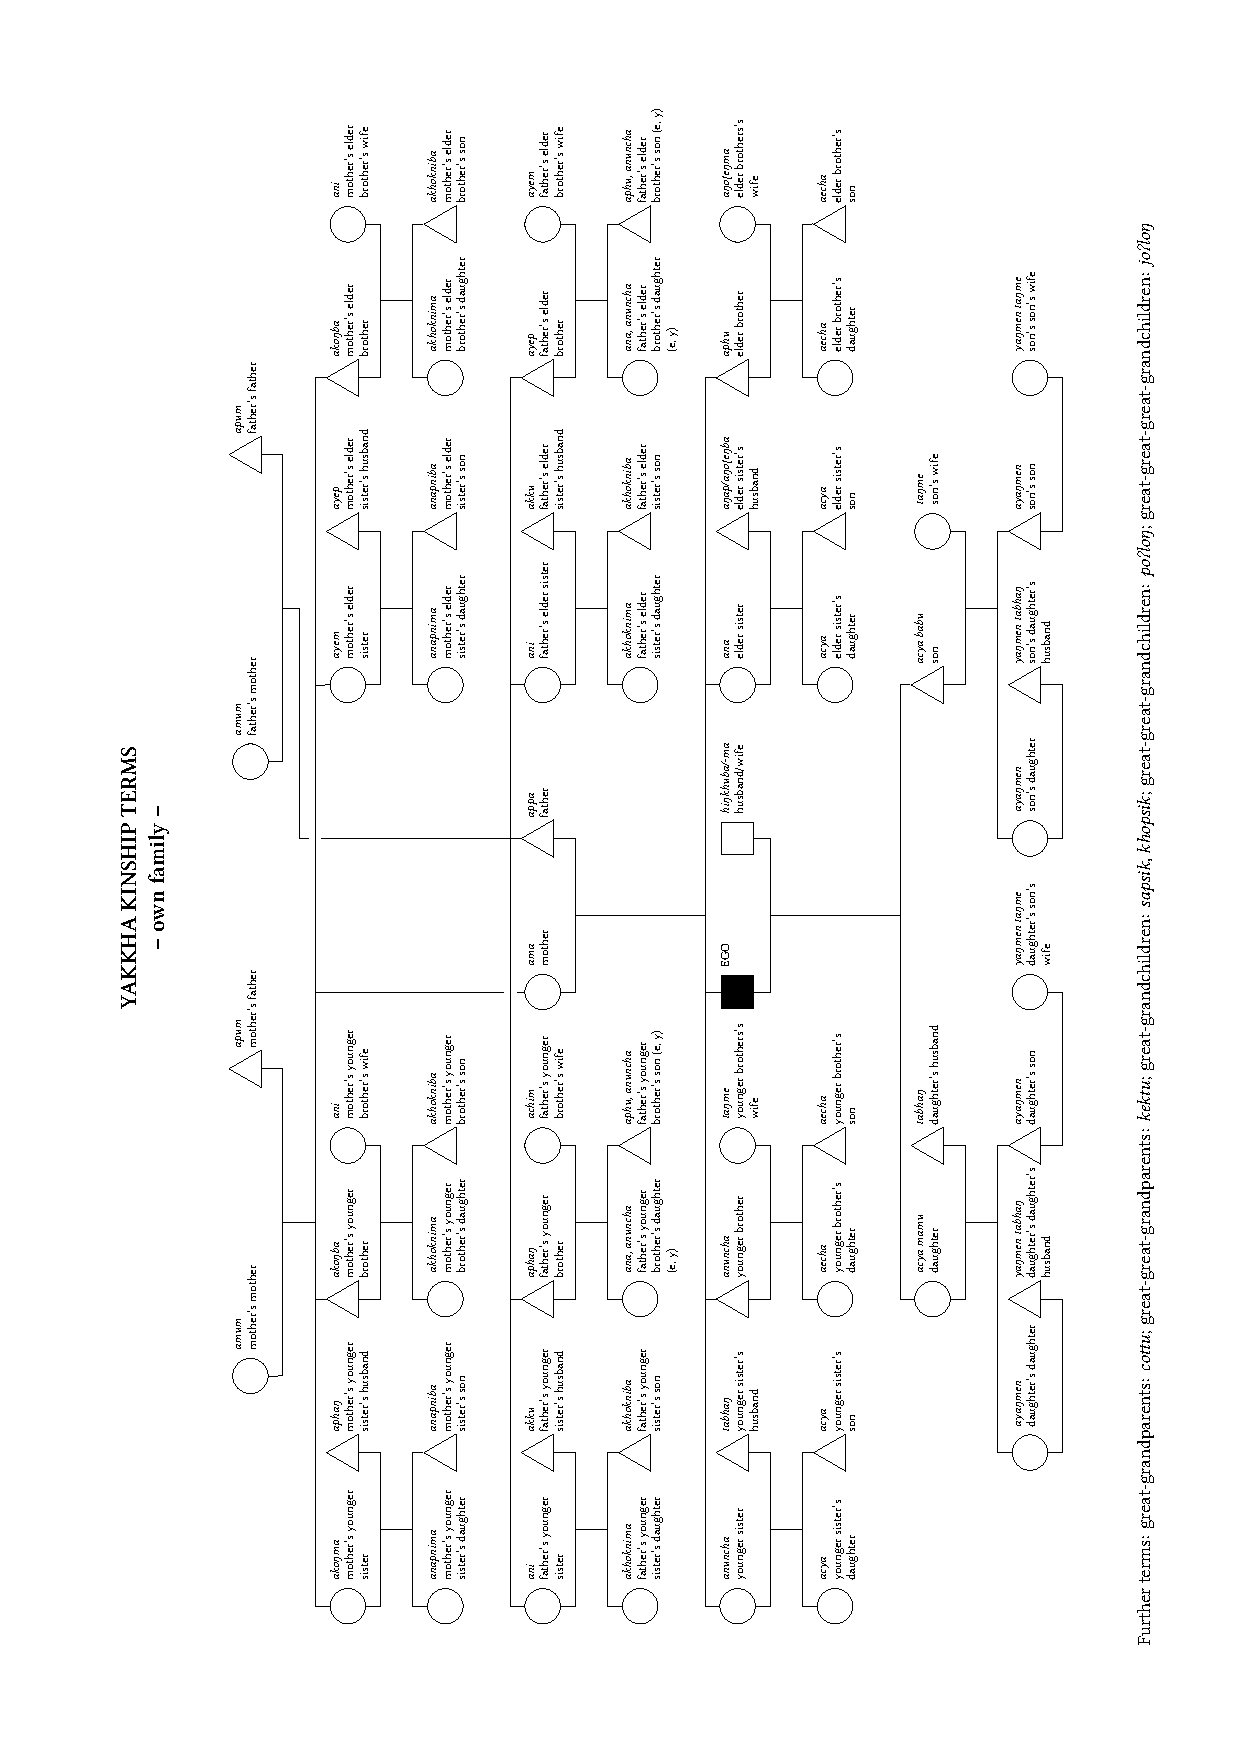
\includepdf{figures/90Grad_Verwandtschaft_eigeneFamilie_zum_Einbinden.pdf}
\cleardoubleemptypage
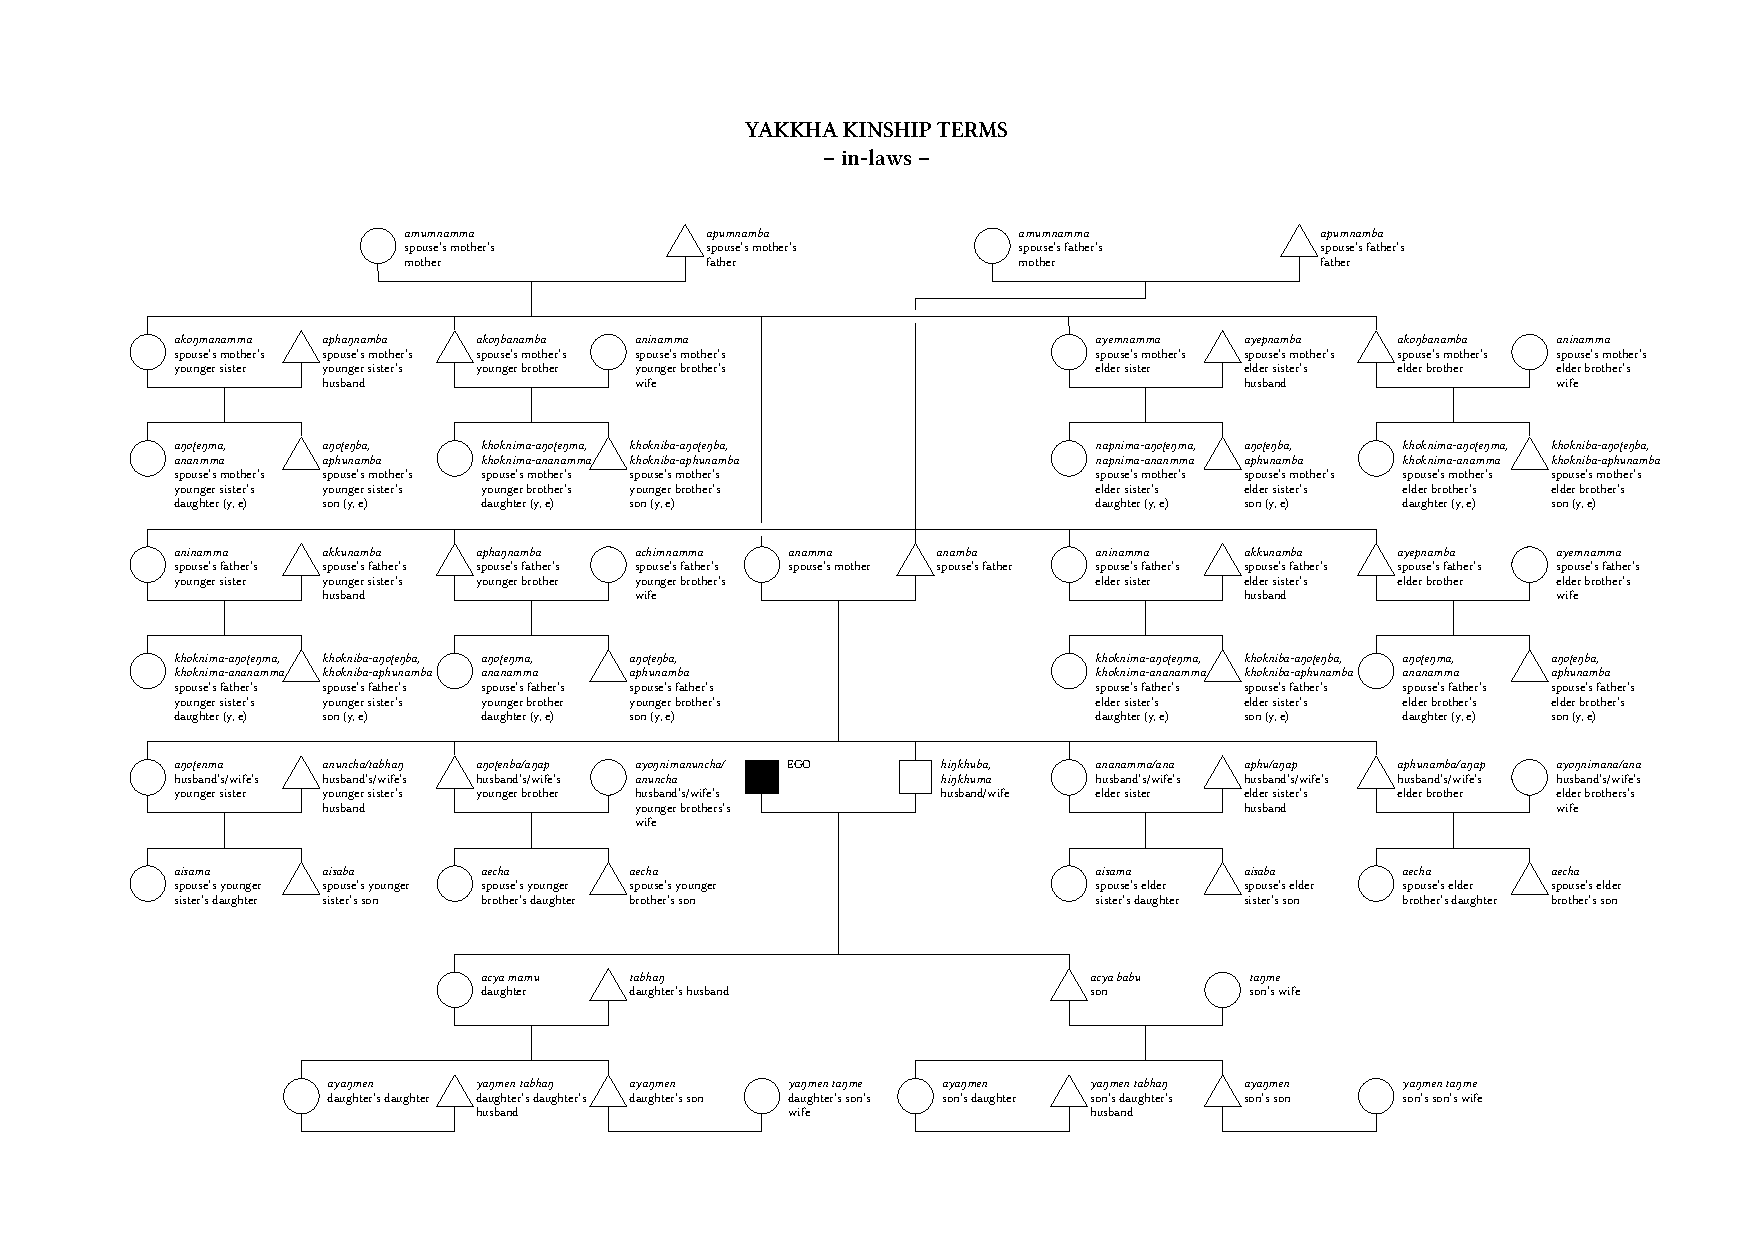
\includepdf{figures/90Grad_Verwandtschaft_Schwiegerfamilie_zum_Einbinden.pdf}


\addchap{Index of Yakkha formatives}

%\addcontentsline{toc}{chapter}{Index of Yakkha formatives}\markboth{Index of Yakkha formatives}{Index of Yakkha formatives}

\begin{centering}
\begin{tabular}{lll}
\lsptoprule
{\sc marker}&{\sc function} & {\sc section}\\
\midrule
\emph{a-}&possessive prefix, {\sc 1sg}&\ref{poss-pron}\\
\emph{-a}&past&\ref{tense}\\
\emph{-a}&imperative, subjunctive&\ref{mood}\\
\emph{-a}&nativizer on loans&\ref{furtherverbal}\\
\emph{-a \ti -na}&function verb, \rede{leave}&\ref{V2-leave}\\
\emph{-ap}&function verb, \rede{come}&\ref{V2-come}\\
\emph{-apt}&function verb, \rede{bring}&\ref{V2-bring}\\
\emph{anciŋ-}&possessive prefix, {\sc 1du.excl}&\ref{poss-pron}\\
\emph{aniŋ-}&possessive prefix, {\sc 1pl.excl}&\ref{poss-pron}\\
\emph{au}&initiative particle&\ref{ptcl-excla}\\
\emph{baŋna}&complementizer&\ref{noun-compl}\\
\emph{baŋha}&complementizer&\ref{noun-compl}\\
\emph{baŋniŋ}&textual topic, quotative&\ref{ptcl-top}\\
\emph{-bhes}&function verb, \rede{deliver}&\ref{V2-bhes}\\
\emph{-bhoks \ti -bhoŋ}&function verb, \rede{split}&\ref{V2-split}\\
\emph{bhoŋ}&conditional, complementizer, quotative&\ref{fin-comp}, \ref{adv-cl-cond}, \ref{adv-cl-fin-purp}\\
\emph{-ca}&function verb, middle, reflexive&\ref{V2-eat}, \ref{refl}\\
\emph{ca}&auxiliary, reciprocal&\ref{refl}\\
\emph{=ca}&additive focus&\ref{ptcl-foc}, \ref{adv-cl-conc}\\
\emph{=chen}&topic&\ref{ptcl-top}\\
\emph{-ci \ti -cin}&dual (verbal)&\ref{verb-infl}\\
\emph{-ci}&3 nonsingular P (verbal)&\ref{verb-infl}\\
\emph{=ci}&nonsingular (nominal)&\ref{number}\\
\emph{-eba}&polite imperative&\ref{mood}\\
\emph{=em}&alternation particle&\ref{ptcl-alt}\\
\emph{eN-}&possessive prefix, {\sc 1pl.incl}&\ref{poss-pron}\\
\emph{-end}&function verb, \rede{insert}&\ref{V2-insert}\\
\emph{enciŋ-}&possessive prefix, {\sc 1du.incl}&\ref{poss-pron}\\
\emph{=ge \ti =ghe}&locative&\ref{case}\\
\emph{-get}&function verb, \rede{bring up}&\ref{V2-bringup}\\
\emph{=gaŋ \ti =ghaŋ}&ablative&\ref{case}\\
\emph{-ghet \ti -het}&function verb, \rede{carry off}&\ref{V2-carryoff}\\
\emph{-ghond}&function verb, \rede{roam}&\ref{V2-roam}\\
\emph{=ha \ti =ya}&nominalizer, {\sc nsg/nc}&\ref{nmlz-uni}\\
\emph{-haks \ti -nhaŋ}&function verb, \rede{send}&\ref{V2-send}\\
\emph{haksaŋ}&comparative&\ref{postpos}\\
\emph{haʔniŋ}&comparative&\ref{postpos}\\
\emph{-heks}&function verb, \rede{cut}&\ref{V2-cut}\\
\emph{=hoŋ}&sequential clause linkage&\ref{adv-cl-seq}, \ref{adv-cl-conc}\\
\emph{=hoŋca}& concessive clause linkage&\ref{adv-cl-conc}\\
\emph{hau}&exclamative&\ref{ptcl-excla}\\
\emph{=i}&sentential focus&\ref{ptcl-foc}\\
\emph{i}&question marker&\ref{ptcl-q}\\
\emph{-i \ti -ni}&completive&\ref{completive}, \ref{V2-compl}\\
\emph{-i \ti -in}&{\sc 1pl, 2pl} (verbal)&\ref{verb-infl}\\
\emph{-ka}&2nd person (verbal)&\ref{verb-infl}\\
\emph{=ka}&genitive&\ref{case}, \ref{maga}\\
\emph{=khaʔla}&directional, manner&\ref{postpos}\\
\emph{-kheʔ}&function verb, \rede{go}&\ref{V2-go}\\
\emph{-khuba}&nominalizer&\ref{nmlz-khuba}\\
\emph{-khusa}&reciprocal marker&\ref{refl}\\
\emph{=ko}&topic&\ref{ptcl-top}\\
\emph{=lai}&exclamative&\ref{ptcl-excla}\\
\emph{=le}&contrastive focus&\ref{ptcl-foc}\\
\emph{-les}&suffix of knowledge or ability&\ref{furtherverbal}\\
\emph{-lo}&interruptive clause linkage&\ref{adv-cl-int}\\
\emph{loppi}&probability&\ref{ptcl-evid}\\
\emph{-loʔa}&equative&\ref{postpos}\\
%\emph{lu}&initiative particle&\ref{}\\
\emph{-m}&{\sc 1pl.A>3, 2pl.A>3 }&\ref{verb-infl}\\
\emph{-ma}&infinitive&\ref{nonfiniteforms}, \ref{nonfin-comp}, \ref{maga}, \ref{manga}\\
\emph{-ma}&event numeral, \rede{times}&\ref{sec-num}\\
\emph{-ma}&nominalizer &\ref{nmlz-pa}\\
\emph{-ma \ti -mi}&perfect&\ref{tense}\\
\emph{=maŋ}&emphatic particle&\ref{ptcl-foc}\\
\emph{-masa \ti -misi}&past perfect&\ref{tense}\\
\emph{maʔniŋ}&privative&\ref{postpos}\\
\emph{meN-}&negation &\ref{neg}\\
\emph{meN-...-le}&negative converb&\ref{menle}\\
\emph{-met}&causative&\ref{caus}\\
\emph{-meʔ}&nonpast&\ref{tense}\\
\emph{N-}&negation (verbal) &\ref{neg}\\
\emph{N-}&{\sc 3pl} &\ref{verb-infl}\\
\emph{N-}&possessive prefix, {\sc 2sg}&\ref{poss-pron}\\
\emph{-n}&negation&\ref{neg}\\
\emph{=na}&nominalizer, {\sc sg}&\ref{nmlz-uni}\\
\emph{-nen}&1>2 (verbal)&\ref{verb-infl}\\
\emph{-nes}&function verb, \rede{lay}&\ref{V2-lay}\\
\emph{-nhaŋto}&temporal ablative&\ref{postpos}\\
\emph{-ni}&optative&\ref{mood}\\
\emph{-nin}&plural and negation (verbal)&\ref{neg}, \ref{verb-infl}\\
\emph{njiŋ-}&possessive prefix, {\sc 2du}&\ref{poss-pron}\\
\emph{=niŋ \ti =niŋa}&cotemporal clause linkage&\ref{sim-finite}\\
\emph{=niŋgobi}&counterfactual clause linkage&\ref{adv-cl-count}\\
\emph{nniŋ-}&possessive prefix, {\sc 2pl}&\ref{poss-pron}\\
\emph{=nuŋ}&comitative case and clause linkage&\ref{case}, \ref{com-cl}\\
\emph{-ŋ \ti -ŋa}&{\sc 1sg, excl}&\ref{verb-infl}\\
\emph{=ŋa}&ergative case and clause linkage&\ref{case}, \ref{manga}\\
\emph{-pa}&nominalizer&\ref{nmlz-pa}\\
\emph{=pa}&sentential focus&\ref{ptcl-foc}\\
\emph{-paŋ}&numeral classifier &\ref{sec-num}\\
\emph{=pe}&locative&\ref{case}\\
\emph{=phaŋ}&ablative&\ref{case}\\
\emph{=pi}&irrealis&\ref{ptcl-evid}\\
\emph{-piʔ}&function verb, \rede{give}&\ref{V2-give}, \ref{benefactive}\\
\emph{=pu}&reportative marker&\ref{ptcl-evid}\\
\emph{rahecha}&mirative&\ref{ptcl-evid}\\
\emph{-raʔ}&function verb, \rede{come}&\ref{V2-comeneut}\\
\emph{-raʔ}&function verb, \rede{bring}&\ref{V2-bringneut}\\
\emph{-ris}&function verb, \rede{place}&\ref{V2-place}\\
\emph{-sa}&infinitive&\ref{nonfiniteforms}, \ref{nonfin-comp}\\
\emph{-saŋ}&simultaneous converb&\ref{sim}\\
\emph{-se}&supine converb&\ref{sup}\\
\emph{=se}&restrictive focus&\ref{ptcl-foc}\\
\emph{-siʔ}&progressive&\ref{progressive}\\
\emph{-siʔ}&middle&\ref{V2-mddl}, \ref{middle}\\
\emph{-siʔ}&function verb, \rede{avoid}&\ref{V2-avoid}\\
\emph{-soʔ}&function verb, \rede{look}&\ref{V2-look}\\
\emph{-t}&benefactive&\ref{benefactive}\\
\emph{u-}&possessive prefix, {\sc 3sg}&\ref{poss-pron}\\
\emph{-u}&3.P (verbal)&\ref{verb-infl}\\
\emph{=u}&vocative&\ref{ptcl-further}\\
\emph{-uks}& function verb, \rede{come down}&\ref{V2-comedown}\\
\emph{-uks \ti -nuŋ}& perfect&\ref{tense}\\
\emph{-uks \ti -nuŋ}& function verb, continuative&\ref{V2-nung}\\
\emph{-uks \ti -uksa}&past perfect&\ref{tense}\\
\emph{-ukt}& function verb, \rede{bring down}&\ref{V2-bringdown}\\
\emph{uŋci-}&possessive prefix, {\sc 3nsg}&\ref{poss-pron}\\
\emph{-wa}&nonpast&\ref{tense}\\
%\emph{-yukt}&function verb, \rede{keep for}&\ref{}\\ only 1 example, not treated, maybe lexical
\emph{=ʔlo}&exclamative&\ref{ptcl-excla}\\
\end{longtable}
\end{centering}







\nocite{Bickel1996Aspect}

\nocite{Bickel1993Belhare}

\nocite{Bickel1998Rhythm} 

\nocite{Bickel1999Nominalization}

\nocite{Bickel1999Grammatical}

\nocite{Bickel2000On-the-syntax}

\nocite{LaPolla1992Dating}

\nocite{Driem1987A-grammar}

\nocite{Driem2001Languages}

\nocite{Hildebrandt2007Prosodic}

\nocite{Polinskyetal1999Agreement}

\nocite{Haspelmath1999Long-distance}

\nocite{Ebert1999Nonfinite}

\nocite{Ebert1993Kiranti}

\nocite{Ebert2003Equivalents}

\nocite{Ebert1994The-structure}

\nocite{Dixon1994Ergativity}
 




 

%%%%%%%%%%%%%%%%%%%%%%%%%%%%%%%%%%%%%%%%%%%%%%%%%%%%
%%%                                              %%%
%%%             Backmatter                       %%%
%%%                                              %%%
%%%%%%%%%%%%%%%%%%%%%%%%%%%%%%%%%%%%%%%%%%%%%%%%%%%%

% There is normally no need to change the backmatter section
 
\phantomsection%this allows hyperlink in ToC to work
% \addcontentsline{toc}{chapter}{List of references}
\printbibliography[heading=references] 
 

\phantomsection 
\addcontentsline{toc}{chapter}{Index} 
\addcontentsline{toc}{section}{Name index}
\ohead{Name index} 
\printindex 
  
\phantomsection 
\addcontentsline{toc}{section}{Language index}
\ohead{Language index} 
\printindex[lan] 
  
\phantomsection 
\addcontentsline{toc}{section}{Subject index}
\ohead{Subject index} 
\printindex[sbj]

\end{document} 


% you can create your book by running
% xelatex lsp-skeleton.tex
%
% you can also try a simple 
% make
% on the commandline
